\documentclass[twoside]{book}

% Packages required by doxygen
\usepackage{fixltx2e}
\usepackage{calc}
\usepackage{doxygen}
\usepackage[export]{adjustbox} % also loads graphicx
\usepackage{graphicx}
\usepackage[utf8]{inputenc}
\usepackage{makeidx}
\usepackage{multicol}
\usepackage{multirow}
\PassOptionsToPackage{warn}{textcomp}
\usepackage{textcomp}
\usepackage[nointegrals]{wasysym}
\usepackage[table]{xcolor}

% Font selection
\usepackage[T1]{fontenc}
\usepackage[scaled=.90]{helvet}
\usepackage{courier}
\usepackage{amssymb}
\usepackage{sectsty}
\renewcommand{\familydefault}{\sfdefault}
\allsectionsfont{%
  \fontseries{bc}\selectfont%
  \color{darkgray}%
}
\renewcommand{\DoxyLabelFont}{%
  \fontseries{bc}\selectfont%
  \color{darkgray}%
}
\newcommand{\+}{\discretionary{\mbox{\scriptsize$\hookleftarrow$}}{}{}}

% Page & text layout
\usepackage{geometry}
\geometry{%
  a4paper,%
  top=2.5cm,%
  bottom=2.5cm,%
  left=2.5cm,%
  right=2.5cm%
}
\tolerance=750
\hfuzz=15pt
\hbadness=750
\setlength{\emergencystretch}{15pt}
\setlength{\parindent}{0cm}
\setlength{\parskip}{3ex plus 2ex minus 2ex}
\makeatletter
\renewcommand{\paragraph}{%
  \@startsection{paragraph}{4}{0ex}{-1.0ex}{1.0ex}{%
    \normalfont\normalsize\bfseries\SS@parafont%
  }%
}
\renewcommand{\subparagraph}{%
  \@startsection{subparagraph}{5}{0ex}{-1.0ex}{1.0ex}{%
    \normalfont\normalsize\bfseries\SS@subparafont%
  }%
}
\makeatother

% Headers & footers
\usepackage{fancyhdr}
\pagestyle{fancyplain}
\fancyhead[LE]{\fancyplain{}{\bfseries\thepage}}
\fancyhead[CE]{\fancyplain{}{}}
\fancyhead[RE]{\fancyplain{}{\bfseries\leftmark}}
\fancyhead[LO]{\fancyplain{}{\bfseries\rightmark}}
\fancyhead[CO]{\fancyplain{}{}}
\fancyhead[RO]{\fancyplain{}{\bfseries\thepage}}
\fancyfoot[LE]{\fancyplain{}{}}
\fancyfoot[CE]{\fancyplain{}{}}
\fancyfoot[RE]{\fancyplain{}{\bfseries\scriptsize Generated by Doxygen }}
\fancyfoot[LO]{\fancyplain{}{\bfseries\scriptsize Generated by Doxygen }}
\fancyfoot[CO]{\fancyplain{}{}}
\fancyfoot[RO]{\fancyplain{}{}}
\renewcommand{\footrulewidth}{0.4pt}
\renewcommand{\chaptermark}[1]{%
  \markboth{#1}{}%
}
\renewcommand{\sectionmark}[1]{%
  \markright{\thesection\ #1}%
}

% Indices & bibliography
\usepackage{natbib}
\usepackage[titles]{tocloft}
\setcounter{tocdepth}{3}
\setcounter{secnumdepth}{5}
\makeindex

% Hyperlinks (required, but should be loaded last)
\usepackage{ifpdf}
\ifpdf
  \usepackage[pdftex,pagebackref=true]{hyperref}
\else
  \usepackage[ps2pdf,pagebackref=true]{hyperref}
\fi
\hypersetup{%
  colorlinks=true,%
  linkcolor=blue,%
  citecolor=blue,%
  unicode%
}

% Custom commands
\newcommand{\clearemptydoublepage}{%
  \newpage{\pagestyle{empty}\cleardoublepage}%
}

\usepackage{caption}
\captionsetup{labelsep=space,justification=centering,font={bf},singlelinecheck=off,skip=4pt,position=top}

%===== C O N T E N T S =====

\begin{document}

% Titlepage & ToC
\hypersetup{pageanchor=false,
             bookmarksnumbered=true,
             pdfencoding=unicode
            }
\pagenumbering{alph}
\begin{titlepage}
\vspace*{7cm}
\begin{center}%
{\Large Mesh Generation Framework }\\
\vspace*{1cm}
{\large Generated by Doxygen 1.8.13}\\
\end{center}
\end{titlepage}
\clearemptydoublepage
\pagenumbering{roman}
\tableofcontents
\clearemptydoublepage
\pagenumbering{arabic}
\hypersetup{pageanchor=true}

%--- Begin generated contents ---
\chapter{Documentation for Mesh\+Generation-\/\+Framework}
\label{md_doc_README}
\Hypertarget{md_doc_README}
Doxygen was used to generate the documentation


\begin{DoxyItemize}
\item The code documentation in H\-T\-M\-L format can be found \href{https://turbulence-master.github.io/Doc-MeshGeneration-Framework/index.html}{\tt here }.
\item The code documentation in La\-Te\-X format can be found at \char`\"{}doc/doxygen/\-H\-T\-M\-L/latex/\char`\"{}. It can be compiled with \char`\"{}make\char`\"{} to generate P\-D\-F(simply navigate to the \char`\"{}/doc/doxygen/\-H\-T\-M\-L/latex/\char`\"{} and type \char`\"{}make\char`\"{}, the generated P\-D\-F file is \char`\"{}refman.\-pdf\char`\"{} in the same directory). 
\end{DoxyItemize}
\chapter{Mesh\+Generation-\/\+Framework}
\label{md_README}
\Hypertarget{md_README}
Mesh Generation Framework as a part of Fortran Project by I\-M\-P Turbulence 2019 Batch

{\bfseries Mesh with a special streching on wall normal direction}



\subsubsection*{Compilation}


\begin{DoxyItemize}
\item Go to build directory \-: cd build rm -\/f C\-Make\-Cache.\-txt
\item Create Makefile with one of these command choosing compiler (gfortran, ifort, ...) and build type (Debug, Release, ...).
\begin{DoxyItemize}
\item To compile with compiler Release flags only {\ttfamily F\-C=gfortran cmake -\/\-D P\-L\-A\-T\-F\-R\-O\-M\-\_\-\-N\-A\-M\-E=lmlm6-\/75 C\-M\-A\-K\-E\-\_\-\-B\-U\-I\-L\-D\-\_\-\-T\-Y\-P\-E=Debug ..} {\ttfamily F\-C=mpif90.\-openmpi cmake -\/\-D P\-L\-A\-T\-F\-R\-O\-M\-\_\-\-N\-A\-M\-E=lmlm6-\/75 C\-M\-A\-K\-E\-\_\-\-B\-U\-I\-L\-D\-\_\-\-T\-Y\-P\-E=Debug ..}
\item To compile with compiler Debug flags only {\ttfamily F\-C=mpif90 cmake -\/\-D C\-M\-A\-K\-E\-\_\-\-B\-U\-I\-L\-D\-\_\-\-T\-Y\-P\-E=Debug -\/\-D P\-L\-A\-T\-F\-R\-O\-M\-\_\-\-N\-A\-M\-E=lmlm6-\/75 -\/\-D\-D\-E\-F\-I\-N\-E\-\_\-\-D\-E\-B\-U\-G=O\-F\-F ..}
\item To compile with D\-E\-B\-U\-G preprocessor option, saves, prints more {\ttfamily F\-C=mpif90 cmake -\/\-D C\-M\-A\-K\-E\-\_\-\-B\-U\-I\-L\-D\-\_\-\-T\-Y\-P\-E=Debug -\/\-D P\-L\-A\-T\-F\-R\-O\-M\-\_\-\-N\-A\-M\-E=lmlm6-\/75 -\/\-D\-D\-E\-F\-I\-N\-E\-\_\-\-D\-E\-B\-U\-G=O\-N ..}
\end{DoxyItemize}
\item Compile {\ttfamily make}
\item Run tests, you should be on the build folder
\begin{DoxyItemize}
\item Run the tests without Fruit outputs  {\ttfamily make test}
\item Run the tests with Fruit outputs {\ttfamily make test A\-R\-G\-S=\char`\"{}-\/\-V\char`\"{}}
\end{DoxyItemize}
\item Clean {\ttfamily make distclean}
\end{DoxyItemize}

\subsubsection*{How to use}


\begin{DoxyItemize}
\item Add shared libraries in your current terminal {\ttfamily L\-I\-B\-Sloc=\char`\"{}/home/solak/\-Workdir/tempdir/\-Workdir/fortan\-\_\-project/my\-Lib/hdf5\char`\"{}} {\ttfamily export L\-D\-\_\-\-L\-I\-B\-R\-A\-R\-Y\-\_\-\-P\-A\-T\-H=\char`\"{}\$\{\-L\-I\-B\-Sloc\}/lib\char`\"{}}
\end{DoxyItemize}

\subsubsection*{Contributing}


\begin{DoxyItemize}
\item {\itshape Make sure you comment each and every block/object/class and every damn variable}
\item {\itshape P\-L\-E\-A\-S\-E D\-O N\-O\-T U\-S\-E S\-P\-A\-C\-E\-S, U\-S\-E H\-Y\-P\-H\-E\-N\-S(-\/) or U\-N\-D\-E\-R\-S\-C\-O\-R\-E\-S(\-\_\-) F\-O\-R F\-I\-L\-E\-N\-A\-M\-E\-S}
\end{DoxyItemize}

\subsubsection*{License}
\chapter{References for the Mesh\+Generation Framework}
\label{md_references_README}
\Hypertarget{md_references_README}
Please upload programs or any other reading material in this directory.

{\itshape P\+L\+E\+A\+SE DO N\+OT U\+SE S\+P\+A\+C\+ES, U\+SE H\+Y\+P\+H\+E\+NS(-\/) or U\+N\+D\+E\+R\+S\+C\+O\+R\+E\+S(\+\_\+) F\+OR F\+I\+L\+E\+N\+A\+M\+ES}

{\itshape T\+H\+IS D\+I\+R\+E\+C\+T\+O\+RY W\+I\+LL BE R\+E\+M\+O\+V\+ED AT T\+HE E\+ND OF P\+R\+O\+J\+E\+CT} 
\chapter{To Do List}
\label{md_src_mesh_formats_README}
\Hypertarget{md_src_mesh_formats_README}

\begin{DoxyEnumerate}
\item Modularise vtk test code
\item test unofficial fortran api / official py2fort bindings for H\+D\+F5 
\end{DoxyEnumerate}
\chapter{Namespace Index}
\section{Namespace List}
Here is a list of all documented namespaces with brief descriptions\+:\begin{DoxyCompactList}
\item\contentsline{section}{\hyperlink{namespaceh5py__LOCAL_1_1__hl_1_1compat}{h5py\+\_\+\+L\+O\+C\+A\+L.\+\_\+hl.\+compat} }{\pageref{namespaceh5py__LOCAL_1_1__hl_1_1compat}}{}
\item\contentsline{section}{\hyperlink{namespaceh5py__LOCAL_1_1tests_1_1hl_1_1test__datatype}{h5py\+\_\+\+L\+O\+C\+A\+L.\+tests.\+hl.\+test\+\_\+datatype} }{\pageref{namespaceh5py__LOCAL_1_1tests_1_1hl_1_1test__datatype}}{}
\end{DoxyCompactList}

\chapter{Hierarchical Index}
\section{Class Hierarchy}
This inheritance list is sorted roughly, but not completely, alphabetically\+:\begin{DoxyCompactList}
\item Items\+View\begin{DoxyCompactList}
\item \contentsline{section}{h5py\+\_\+\+L\+O\+C\+A\+L.\+\_\+hl.\+base.\+Items\+View\+H\+D\+F5}{\pageref{classh5py__LOCAL_1_1__hl_1_1base_1_1ItemsViewHDF5}}{}
\end{DoxyCompactList}
\item Mapping\begin{DoxyCompactList}
\item \contentsline{section}{h5py\+\_\+\+L\+O\+C\+A\+L.\+\_\+hl.\+base.\+Mapping\+H\+D\+F5}{\pageref{classh5py__LOCAL_1_1__hl_1_1base_1_1MappingHDF5}}{}
\begin{DoxyCompactList}
\item \contentsline{section}{h5py\+\_\+\+L\+O\+C\+A\+L.\+\_\+hl.\+base.\+Mutable\+Mapping\+H\+D\+F5}{\pageref{classh5py__LOCAL_1_1__hl_1_1base_1_1MutableMappingHDF5}}{}
\begin{DoxyCompactList}
\item \contentsline{section}{h5py\+\_\+\+L\+O\+C\+A\+L.\+\_\+hl.\+attrs.\+Attribute\+Manager}{\pageref{classh5py__LOCAL_1_1__hl_1_1attrs_1_1AttributeManager}}{}
\item \contentsline{section}{h5py\+\_\+\+L\+O\+C\+A\+L.\+\_\+hl.\+group.\+Group}{\pageref{classh5py__LOCAL_1_1__hl_1_1group_1_1Group}}{}
\begin{DoxyCompactList}
\item \contentsline{section}{h5py\+\_\+\+L\+O\+C\+A\+L.\+\_\+hl.\+files.\+File}{\pageref{classh5py__LOCAL_1_1__hl_1_1files_1_1File}}{}
\end{DoxyCompactList}
\end{DoxyCompactList}
\item \contentsline{section}{h5py\+\_\+\+L\+O\+C\+A\+L.\+\_\+hl.\+dims.\+Dimension\+Manager}{\pageref{classh5py__LOCAL_1_1__hl_1_1dims_1_1DimensionManager}}{}
\end{DoxyCompactList}
\end{DoxyCompactList}
\item \contentsline{section}{class\+\_\+mesh\+:\+:mesh\+\_\+grid}{\pageref{structclass__mesh_1_1mesh__grid}}{}
\item Mutable\+Mapping\begin{DoxyCompactList}
\item \contentsline{section}{h5py\+\_\+\+L\+O\+C\+A\+L.\+\_\+hl.\+base.\+Mutable\+Mapping\+H\+D\+F5}{\pageref{classh5py__LOCAL_1_1__hl_1_1base_1_1MutableMappingHDF5}}{}
\end{DoxyCompactList}
\item object\begin{DoxyCompactList}
\item \contentsline{section}{h5py\+\_\+\+L\+O\+C\+A\+L.\+\_\+hl.\+base.\+\_\+\+Region\+Proxy}{\pageref{classh5py__LOCAL_1_1__hl_1_1base_1_1__RegionProxy}}{}
\item \contentsline{section}{h5py\+\_\+\+L\+O\+C\+A\+L.\+\_\+hl.\+base.\+Common\+State\+Object}{\pageref{classh5py__LOCAL_1_1__hl_1_1base_1_1CommonStateObject}}{}
\begin{DoxyCompactList}
\item \contentsline{section}{h5py\+\_\+\+L\+O\+C\+A\+L.\+\_\+hl.\+attrs.\+Attribute\+Manager}{\pageref{classh5py__LOCAL_1_1__hl_1_1attrs_1_1AttributeManager}}{}
\item \contentsline{section}{h5py\+\_\+\+L\+O\+C\+A\+L.\+\_\+hl.\+base.\+H\+L\+Object}{\pageref{classh5py__LOCAL_1_1__hl_1_1base_1_1HLObject}}{}
\begin{DoxyCompactList}
\item \contentsline{section}{h5py\+\_\+\+L\+O\+C\+A\+L.\+\_\+hl.\+dataset.\+Dataset}{\pageref{classh5py__LOCAL_1_1__hl_1_1dataset_1_1Dataset}}{}
\item \contentsline{section}{h5py\+\_\+\+L\+O\+C\+A\+L.\+\_\+hl.\+datatype.\+Datatype}{\pageref{classh5py__LOCAL_1_1__hl_1_1datatype_1_1Datatype}}{}
\item \contentsline{section}{h5py\+\_\+\+L\+O\+C\+A\+L.\+\_\+hl.\+group.\+Group}{\pageref{classh5py__LOCAL_1_1__hl_1_1group_1_1Group}}{}
\end{DoxyCompactList}
\item \contentsline{section}{h5py\+\_\+\+L\+O\+C\+A\+L.\+\_\+hl.\+dims.\+Dimension\+Manager}{\pageref{classh5py__LOCAL_1_1__hl_1_1dims_1_1DimensionManager}}{}
\item \contentsline{section}{h5py\+\_\+\+L\+O\+C\+A\+L.\+\_\+hl.\+dims.\+Dimension\+Proxy}{\pageref{classh5py__LOCAL_1_1__hl_1_1dims_1_1DimensionProxy}}{}
\end{DoxyCompactList}
\item \contentsline{section}{h5py\+\_\+\+L\+O\+C\+A\+L.\+\_\+hl.\+base.\+Empty}{\pageref{classh5py__LOCAL_1_1__hl_1_1base_1_1Empty}}{}
\item \contentsline{section}{h5py\+\_\+\+L\+O\+C\+A\+L.\+\_\+hl.\+dataset.\+Astype\+Context}{\pageref{classh5py__LOCAL_1_1__hl_1_1dataset_1_1AstypeContext}}{}
\item \contentsline{section}{h5py\+\_\+\+L\+O\+C\+A\+L.\+\_\+hl.\+dataset.\+Collective\+Context}{\pageref{classh5py__LOCAL_1_1__hl_1_1dataset_1_1CollectiveContext}}{}
\item \contentsline{section}{h5py\+\_\+\+L\+O\+C\+A\+L.\+\_\+hl.\+group.\+External\+Link}{\pageref{classh5py__LOCAL_1_1__hl_1_1group_1_1ExternalLink}}{}
\item \contentsline{section}{h5py\+\_\+\+L\+O\+C\+A\+L.\+\_\+hl.\+group.\+Hard\+Link}{\pageref{classh5py__LOCAL_1_1__hl_1_1group_1_1HardLink}}{}
\item \contentsline{section}{h5py\+\_\+\+L\+O\+C\+A\+L.\+\_\+hl.\+group.\+Soft\+Link}{\pageref{classh5py__LOCAL_1_1__hl_1_1group_1_1SoftLink}}{}
\item \contentsline{section}{h5py\+\_\+\+L\+O\+C\+A\+L.\+\_\+hl.\+selections2.\+Scalar\+Read\+Selection}{\pageref{classh5py__LOCAL_1_1__hl_1_1selections2_1_1ScalarReadSelection}}{}
\item \contentsline{section}{h5py\+\_\+\+L\+O\+C\+A\+L.\+\_\+hl.\+selections.\+\_\+\+Region\+Proxy}{\pageref{classh5py__LOCAL_1_1__hl_1_1selections_1_1__RegionProxy}}{}
\item \contentsline{section}{h5py\+\_\+\+L\+O\+C\+A\+L.\+\_\+hl.\+selections.\+Selection}{\pageref{classh5py__LOCAL_1_1__hl_1_1selections_1_1Selection}}{}
\begin{DoxyCompactList}
\item \contentsline{section}{h5py\+\_\+\+L\+O\+C\+A\+L.\+\_\+hl.\+selections.\+Fancy\+Selection}{\pageref{classh5py__LOCAL_1_1__hl_1_1selections_1_1FancySelection}}{}
\item \contentsline{section}{h5py\+\_\+\+L\+O\+C\+A\+L.\+\_\+hl.\+selections.\+Point\+Selection}{\pageref{classh5py__LOCAL_1_1__hl_1_1selections_1_1PointSelection}}{}
\item \contentsline{section}{h5py\+\_\+\+L\+O\+C\+A\+L.\+\_\+hl.\+selections.\+Simple\+Selection}{\pageref{classh5py__LOCAL_1_1__hl_1_1selections_1_1SimpleSelection}}{}
\end{DoxyCompactList}
\end{DoxyCompactList}
\item Test\+Case\begin{DoxyCompactList}
\item \contentsline{section}{h5py\+\_\+\+L\+O\+C\+A\+L.\+tests.\+common.\+Test\+Case}{\pageref{classh5py__LOCAL_1_1tests_1_1common_1_1TestCase}}{}
\begin{DoxyCompactList}
\item \contentsline{section}{h5py\+\_\+\+L\+O\+C\+A\+L.\+tests.\+hl.\+test\+\_\+attribute\+\_\+create.\+Test\+Array}{\pageref{classh5py__LOCAL_1_1tests_1_1hl_1_1test__attribute__create_1_1TestArray}}{}
\item \contentsline{section}{h5py\+\_\+\+L\+O\+C\+A\+L.\+tests.\+hl.\+test\+\_\+dataset\+\_\+getitem.\+Test1\+D\+Float}{\pageref{classh5py__LOCAL_1_1tests_1_1hl_1_1test__dataset__getitem_1_1Test1DFloat}}{}
\item \contentsline{section}{h5py\+\_\+\+L\+O\+C\+A\+L.\+tests.\+hl.\+test\+\_\+dataset\+\_\+getitem.\+Test1\+D\+Zero\+Float}{\pageref{classh5py__LOCAL_1_1tests_1_1hl_1_1test__dataset__getitem_1_1Test1DZeroFloat}}{}
\item \contentsline{section}{h5py\+\_\+\+L\+O\+C\+A\+L.\+tests.\+hl.\+test\+\_\+dataset\+\_\+getitem.\+Test2\+D\+Zero\+Float}{\pageref{classh5py__LOCAL_1_1tests_1_1hl_1_1test__dataset__getitem_1_1Test2DZeroFloat}}{}
\item \contentsline{section}{h5py\+\_\+\+L\+O\+C\+A\+L.\+tests.\+hl.\+test\+\_\+dataset\+\_\+getitem.\+Test\+Empty}{\pageref{classh5py__LOCAL_1_1tests_1_1hl_1_1test__dataset__getitem_1_1TestEmpty}}{}
\item \contentsline{section}{h5py\+\_\+\+L\+O\+C\+A\+L.\+tests.\+hl.\+test\+\_\+dataset\+\_\+getitem.\+Test\+Scalar\+Array}{\pageref{classh5py__LOCAL_1_1tests_1_1hl_1_1test__dataset__getitem_1_1TestScalarArray}}{}
\item \contentsline{section}{h5py\+\_\+\+L\+O\+C\+A\+L.\+tests.\+hl.\+test\+\_\+dataset\+\_\+getitem.\+Test\+Scalar\+Compound}{\pageref{classh5py__LOCAL_1_1tests_1_1hl_1_1test__dataset__getitem_1_1TestScalarCompound}}{}
\item \contentsline{section}{h5py\+\_\+\+L\+O\+C\+A\+L.\+tests.\+hl.\+test\+\_\+dataset\+\_\+getitem.\+Test\+Scalar\+Float}{\pageref{classh5py__LOCAL_1_1tests_1_1hl_1_1test__dataset__getitem_1_1TestScalarFloat}}{}
\item \contentsline{section}{h5py\+\_\+\+L\+O\+C\+A\+L.\+tests.\+hl.\+test\+\_\+dataset\+\_\+getitem.\+Test\+Very\+Large\+Array}{\pageref{classh5py__LOCAL_1_1tests_1_1hl_1_1test__dataset__getitem_1_1TestVeryLargeArray}}{}
\item \contentsline{section}{h5py\+\_\+\+L\+O\+C\+A\+L.\+tests.\+hl.\+test\+\_\+dataset\+\_\+swmr.\+Test\+Dataset\+Swmr\+Read}{\pageref{classh5py__LOCAL_1_1tests_1_1hl_1_1test__dataset__swmr_1_1TestDatasetSwmrRead}}{}
\item \contentsline{section}{h5py\+\_\+\+L\+O\+C\+A\+L.\+tests.\+hl.\+test\+\_\+dataset\+\_\+swmr.\+Test\+Dataset\+Swmr\+Write}{\pageref{classh5py__LOCAL_1_1tests_1_1hl_1_1test__dataset__swmr_1_1TestDatasetSwmrWrite}}{}
\item \contentsline{section}{h5py\+\_\+\+L\+O\+C\+A\+L.\+tests.\+hl.\+test\+\_\+dataset\+\_\+swmr.\+Test\+Swmr\+Not\+Available}{\pageref{classh5py__LOCAL_1_1tests_1_1hl_1_1test__dataset__swmr_1_1TestSwmrNotAvailable}}{}
\item \contentsline{section}{h5py\+\_\+\+L\+O\+C\+A\+L.\+tests.\+hl.\+test\+\_\+datatype.\+Test\+Offsets}{\pageref{classh5py__LOCAL_1_1tests_1_1hl_1_1test__datatype_1_1TestOffsets}}{}
\item \contentsline{section}{h5py\+\_\+\+L\+O\+C\+A\+L.\+tests.\+hl.\+test\+\_\+datatype.\+Test\+Vlen}{\pageref{classh5py__LOCAL_1_1tests_1_1hl_1_1test__datatype_1_1TestVlen}}{}
\item \contentsline{section}{h5py\+\_\+\+L\+O\+C\+A\+L.\+tests.\+hl.\+test\+\_\+dims\+\_\+dimensionproxy.\+Test\+Items}{\pageref{classh5py__LOCAL_1_1tests_1_1hl_1_1test__dims__dimensionproxy_1_1TestItems}}{}
\item \contentsline{section}{h5py\+\_\+\+L\+O\+C\+A\+L.\+tests.\+hl.\+test\+\_\+file.\+Test\+Dealloc}{\pageref{classh5py__LOCAL_1_1tests_1_1hl_1_1test__file_1_1TestDealloc}}{}
\item \contentsline{section}{h5py\+\_\+\+L\+O\+C\+A\+L.\+tests.\+hl.\+test\+\_\+threads.\+Test\+Error\+Printing}{\pageref{classh5py__LOCAL_1_1tests_1_1hl_1_1test__threads_1_1TestErrorPrinting}}{}
\item \contentsline{section}{h5py\+\_\+\+L\+O\+C\+A\+L.\+tests.\+old.\+test\+\_\+attrs.\+Base\+Attrs}{\pageref{classh5py__LOCAL_1_1tests_1_1old_1_1test__attrs_1_1BaseAttrs}}{}
\begin{DoxyCompactList}
\item \contentsline{section}{h5py\+\_\+\+L\+O\+C\+A\+L.\+tests.\+old.\+test\+\_\+attrs.\+Test\+Access}{\pageref{classh5py__LOCAL_1_1tests_1_1old_1_1test__attrs_1_1TestAccess}}{}
\item \contentsline{section}{h5py\+\_\+\+L\+O\+C\+A\+L.\+tests.\+old.\+test\+\_\+attrs.\+Test\+Create}{\pageref{classh5py__LOCAL_1_1tests_1_1old_1_1test__attrs_1_1TestCreate}}{}
\item \contentsline{section}{h5py\+\_\+\+L\+O\+C\+A\+L.\+tests.\+old.\+test\+\_\+attrs.\+Test\+Delete}{\pageref{classh5py__LOCAL_1_1tests_1_1old_1_1test__attrs_1_1TestDelete}}{}
\item \contentsline{section}{h5py\+\_\+\+L\+O\+C\+A\+L.\+tests.\+old.\+test\+\_\+attrs.\+Test\+Mutable\+Mapping}{\pageref{classh5py__LOCAL_1_1tests_1_1old_1_1test__attrs_1_1TestMutableMapping}}{}
\item \contentsline{section}{h5py\+\_\+\+L\+O\+C\+A\+L.\+tests.\+old.\+test\+\_\+attrs.\+Test\+Unicode}{\pageref{classh5py__LOCAL_1_1tests_1_1old_1_1test__attrs_1_1TestUnicode}}{}
\item \contentsline{section}{h5py\+\_\+\+L\+O\+C\+A\+L.\+tests.\+old.\+test\+\_\+attrs.\+Test\+Vlen}{\pageref{classh5py__LOCAL_1_1tests_1_1old_1_1test__attrs_1_1TestVlen}}{}
\end{DoxyCompactList}
\item \contentsline{section}{h5py\+\_\+\+L\+O\+C\+A\+L.\+tests.\+old.\+test\+\_\+attrs\+\_\+data.\+Base\+Attrs}{\pageref{classh5py__LOCAL_1_1tests_1_1old_1_1test__attrs__data_1_1BaseAttrs}}{}
\begin{DoxyCompactList}
\item \contentsline{section}{h5py\+\_\+\+L\+O\+C\+A\+L.\+tests.\+old.\+test\+\_\+attrs\+\_\+data.\+Test\+Array}{\pageref{classh5py__LOCAL_1_1tests_1_1old_1_1test__attrs__data_1_1TestArray}}{}
\item \contentsline{section}{h5py\+\_\+\+L\+O\+C\+A\+L.\+tests.\+old.\+test\+\_\+attrs\+\_\+data.\+Test\+Empty}{\pageref{classh5py__LOCAL_1_1tests_1_1old_1_1test__attrs__data_1_1TestEmpty}}{}
\item \contentsline{section}{h5py\+\_\+\+L\+O\+C\+A\+L.\+tests.\+old.\+test\+\_\+attrs\+\_\+data.\+Test\+Scalar}{\pageref{classh5py__LOCAL_1_1tests_1_1old_1_1test__attrs__data_1_1TestScalar}}{}
\item \contentsline{section}{h5py\+\_\+\+L\+O\+C\+A\+L.\+tests.\+old.\+test\+\_\+attrs\+\_\+data.\+Test\+Types}{\pageref{classh5py__LOCAL_1_1tests_1_1old_1_1test__attrs__data_1_1TestTypes}}{}
\item \contentsline{section}{h5py\+\_\+\+L\+O\+C\+A\+L.\+tests.\+old.\+test\+\_\+attrs\+\_\+data.\+Test\+Write\+Exception}{\pageref{classh5py__LOCAL_1_1tests_1_1old_1_1test__attrs__data_1_1TestWriteException}}{}
\end{DoxyCompactList}
\item \contentsline{section}{h5py\+\_\+\+L\+O\+C\+A\+L.\+tests.\+old.\+test\+\_\+base.\+Base\+Test}{\pageref{classh5py__LOCAL_1_1tests_1_1old_1_1test__base_1_1BaseTest}}{}
\begin{DoxyCompactList}
\item \contentsline{section}{h5py\+\_\+\+L\+O\+C\+A\+L.\+tests.\+old.\+test\+\_\+base.\+Test\+Name}{\pageref{classh5py__LOCAL_1_1tests_1_1old_1_1test__base_1_1TestName}}{}
\item \contentsline{section}{h5py\+\_\+\+L\+O\+C\+A\+L.\+tests.\+old.\+test\+\_\+base.\+Test\+Repr}{\pageref{classh5py__LOCAL_1_1tests_1_1old_1_1test__base_1_1TestRepr}}{}
\end{DoxyCompactList}
\item \contentsline{section}{h5py\+\_\+\+L\+O\+C\+A\+L.\+tests.\+old.\+test\+\_\+dataset.\+Base\+Dataset}{\pageref{classh5py__LOCAL_1_1tests_1_1old_1_1test__dataset_1_1BaseDataset}}{}
\begin{DoxyCompactList}
\item \contentsline{section}{h5py\+\_\+\+L\+O\+C\+A\+L.\+tests.\+old.\+test\+\_\+dataset.\+Test\+Astype}{\pageref{classh5py__LOCAL_1_1tests_1_1old_1_1test__dataset_1_1TestAstype}}{}
\item \contentsline{section}{h5py\+\_\+\+L\+O\+C\+A\+L.\+tests.\+old.\+test\+\_\+dataset.\+Test\+Auto\+Create}{\pageref{classh5py__LOCAL_1_1tests_1_1old_1_1test__dataset_1_1TestAutoCreate}}{}
\item \contentsline{section}{h5py\+\_\+\+L\+O\+C\+A\+L.\+tests.\+old.\+test\+\_\+dataset.\+Test\+Compound}{\pageref{classh5py__LOCAL_1_1tests_1_1old_1_1test__dataset_1_1TestCompound}}{}
\item \contentsline{section}{h5py\+\_\+\+L\+O\+C\+A\+L.\+tests.\+old.\+test\+\_\+dataset.\+Test\+Create\+Chunked}{\pageref{classh5py__LOCAL_1_1tests_1_1old_1_1test__dataset_1_1TestCreateChunked}}{}
\item \contentsline{section}{h5py\+\_\+\+L\+O\+C\+A\+L.\+tests.\+old.\+test\+\_\+dataset.\+Test\+Create\+Compression\+Number}{\pageref{classh5py__LOCAL_1_1tests_1_1old_1_1test__dataset_1_1TestCreateCompressionNumber}}{}
\item \contentsline{section}{h5py\+\_\+\+L\+O\+C\+A\+L.\+tests.\+old.\+test\+\_\+dataset.\+Test\+Create\+Data}{\pageref{classh5py__LOCAL_1_1tests_1_1old_1_1test__dataset_1_1TestCreateData}}{}
\item \contentsline{section}{h5py\+\_\+\+L\+O\+C\+A\+L.\+tests.\+old.\+test\+\_\+dataset.\+Test\+Create\+Fillvalue}{\pageref{classh5py__LOCAL_1_1tests_1_1old_1_1test__dataset_1_1TestCreateFillvalue}}{}
\item \contentsline{section}{h5py\+\_\+\+L\+O\+C\+A\+L.\+tests.\+old.\+test\+\_\+dataset.\+Test\+Create\+Fletcher32}{\pageref{classh5py__LOCAL_1_1tests_1_1old_1_1test__dataset_1_1TestCreateFletcher32}}{}
\item \contentsline{section}{h5py\+\_\+\+L\+O\+C\+A\+L.\+tests.\+old.\+test\+\_\+dataset.\+Test\+Create\+Gzip}{\pageref{classh5py__LOCAL_1_1tests_1_1old_1_1test__dataset_1_1TestCreateGzip}}{}
\item \contentsline{section}{h5py\+\_\+\+L\+O\+C\+A\+L.\+tests.\+old.\+test\+\_\+dataset.\+Test\+Create\+L\+ZF}{\pageref{classh5py__LOCAL_1_1tests_1_1old_1_1test__dataset_1_1TestCreateLZF}}{}
\item \contentsline{section}{h5py\+\_\+\+L\+O\+C\+A\+L.\+tests.\+old.\+test\+\_\+dataset.\+Test\+Create\+Named\+Type}{\pageref{classh5py__LOCAL_1_1tests_1_1old_1_1test__dataset_1_1TestCreateNamedType}}{}
\item \contentsline{section}{h5py\+\_\+\+L\+O\+C\+A\+L.\+tests.\+old.\+test\+\_\+dataset.\+Test\+Create\+Require}{\pageref{classh5py__LOCAL_1_1tests_1_1old_1_1test__dataset_1_1TestCreateRequire}}{}
\item \contentsline{section}{h5py\+\_\+\+L\+O\+C\+A\+L.\+tests.\+old.\+test\+\_\+dataset.\+Test\+Create\+Scale\+Offset}{\pageref{classh5py__LOCAL_1_1tests_1_1old_1_1test__dataset_1_1TestCreateScaleOffset}}{}
\item \contentsline{section}{h5py\+\_\+\+L\+O\+C\+A\+L.\+tests.\+old.\+test\+\_\+dataset.\+Test\+Create\+Shape}{\pageref{classh5py__LOCAL_1_1tests_1_1old_1_1test__dataset_1_1TestCreateShape}}{}
\item \contentsline{section}{h5py\+\_\+\+L\+O\+C\+A\+L.\+tests.\+old.\+test\+\_\+dataset.\+Test\+Create\+Shuffle}{\pageref{classh5py__LOCAL_1_1tests_1_1old_1_1test__dataset_1_1TestCreateShuffle}}{}
\item \contentsline{section}{h5py\+\_\+\+L\+O\+C\+A\+L.\+tests.\+old.\+test\+\_\+dataset.\+Test\+Create\+S\+Z\+IP}{\pageref{classh5py__LOCAL_1_1tests_1_1old_1_1test__dataset_1_1TestCreateSZIP}}{}
\item \contentsline{section}{h5py\+\_\+\+L\+O\+C\+A\+L.\+tests.\+old.\+test\+\_\+dataset.\+Test\+Dtype}{\pageref{classh5py__LOCAL_1_1tests_1_1old_1_1test__dataset_1_1TestDtype}}{}
\item \contentsline{section}{h5py\+\_\+\+L\+O\+C\+A\+L.\+tests.\+old.\+test\+\_\+dataset.\+Test\+Enum}{\pageref{classh5py__LOCAL_1_1tests_1_1old_1_1test__dataset_1_1TestEnum}}{}
\item \contentsline{section}{h5py\+\_\+\+L\+O\+C\+A\+L.\+tests.\+old.\+test\+\_\+dataset.\+Test\+Floats}{\pageref{classh5py__LOCAL_1_1tests_1_1old_1_1test__dataset_1_1TestFloats}}{}
\item \contentsline{section}{h5py\+\_\+\+L\+O\+C\+A\+L.\+tests.\+old.\+test\+\_\+dataset.\+Test\+Iter}{\pageref{classh5py__LOCAL_1_1tests_1_1old_1_1test__dataset_1_1TestIter}}{}
\item \contentsline{section}{h5py\+\_\+\+L\+O\+C\+A\+L.\+tests.\+old.\+test\+\_\+dataset.\+Test\+Len}{\pageref{classh5py__LOCAL_1_1tests_1_1old_1_1test__dataset_1_1TestLen}}{}
\item \contentsline{section}{h5py\+\_\+\+L\+O\+C\+A\+L.\+tests.\+old.\+test\+\_\+dataset.\+Test\+Low\+Open}{\pageref{classh5py__LOCAL_1_1tests_1_1old_1_1test__dataset_1_1TestLowOpen}}{}
\item \contentsline{section}{h5py\+\_\+\+L\+O\+C\+A\+L.\+tests.\+old.\+test\+\_\+dataset.\+Test\+Region\+Refs}{\pageref{classh5py__LOCAL_1_1tests_1_1old_1_1test__dataset_1_1TestRegionRefs}}{}
\item \contentsline{section}{h5py\+\_\+\+L\+O\+C\+A\+L.\+tests.\+old.\+test\+\_\+dataset.\+Test\+Repr}{\pageref{classh5py__LOCAL_1_1tests_1_1old_1_1test__dataset_1_1TestRepr}}{}
\item \contentsline{section}{h5py\+\_\+\+L\+O\+C\+A\+L.\+tests.\+old.\+test\+\_\+dataset.\+Test\+Resize}{\pageref{classh5py__LOCAL_1_1tests_1_1old_1_1test__dataset_1_1TestResize}}{}
\item \contentsline{section}{h5py\+\_\+\+L\+O\+C\+A\+L.\+tests.\+old.\+test\+\_\+dataset.\+Test\+Scalar\+Compound}{\pageref{classh5py__LOCAL_1_1tests_1_1old_1_1test__dataset_1_1TestScalarCompound}}{}
\item \contentsline{section}{h5py\+\_\+\+L\+O\+C\+A\+L.\+tests.\+old.\+test\+\_\+dataset.\+Test\+Strings}{\pageref{classh5py__LOCAL_1_1tests_1_1old_1_1test__dataset_1_1TestStrings}}{}
\item \contentsline{section}{h5py\+\_\+\+L\+O\+C\+A\+L.\+tests.\+old.\+test\+\_\+dataset.\+Test\+Track\+Times}{\pageref{classh5py__LOCAL_1_1tests_1_1old_1_1test__dataset_1_1TestTrackTimes}}{}
\item \contentsline{section}{h5py\+\_\+\+L\+O\+C\+A\+L.\+tests.\+old.\+test\+\_\+dataset.\+Test\+Vlen}{\pageref{classh5py__LOCAL_1_1tests_1_1old_1_1test__dataset_1_1TestVlen}}{}
\item \contentsline{section}{h5py\+\_\+\+L\+O\+C\+A\+L.\+tests.\+old.\+test\+\_\+dataset.\+Test\+Zero\+Shape}{\pageref{classh5py__LOCAL_1_1tests_1_1old_1_1test__dataset_1_1TestZeroShape}}{}
\end{DoxyCompactList}
\item \contentsline{section}{h5py\+\_\+\+L\+O\+C\+A\+L.\+tests.\+old.\+test\+\_\+datatype.\+Base\+Type}{\pageref{classh5py__LOCAL_1_1tests_1_1old_1_1test__datatype_1_1BaseType}}{}
\begin{DoxyCompactList}
\item \contentsline{section}{h5py\+\_\+\+L\+O\+C\+A\+L.\+tests.\+old.\+test\+\_\+datatype.\+Test\+Creation}{\pageref{classh5py__LOCAL_1_1tests_1_1old_1_1test__datatype_1_1TestCreation}}{}
\end{DoxyCompactList}
\item \contentsline{section}{h5py\+\_\+\+L\+O\+C\+A\+L.\+tests.\+old.\+test\+\_\+dimension\+\_\+scales.\+Base\+Dataset}{\pageref{classh5py__LOCAL_1_1tests_1_1old_1_1test__dimension__scales_1_1BaseDataset}}{}
\begin{DoxyCompactList}
\item \contentsline{section}{h5py\+\_\+\+L\+O\+C\+A\+L.\+tests.\+old.\+test\+\_\+dimension\+\_\+scales.\+Test\+Dimension\+Manager}{\pageref{classh5py__LOCAL_1_1tests_1_1old_1_1test__dimension__scales_1_1TestDimensionManager}}{}
\item \contentsline{section}{h5py\+\_\+\+L\+O\+C\+A\+L.\+tests.\+old.\+test\+\_\+dimension\+\_\+scales.\+Test\+Dimensions\+High\+Level}{\pageref{classh5py__LOCAL_1_1tests_1_1old_1_1test__dimension__scales_1_1TestDimensionsHighLevel}}{}
\item \contentsline{section}{h5py\+\_\+\+L\+O\+C\+A\+L.\+tests.\+old.\+test\+\_\+dimension\+\_\+scales.\+Test\+H5\+D\+S\+Bindings}{\pageref{classh5py__LOCAL_1_1tests_1_1old_1_1test__dimension__scales_1_1TestH5DSBindings}}{}
\end{DoxyCompactList}
\item \contentsline{section}{h5py\+\_\+\+L\+O\+C\+A\+L.\+tests.\+old.\+test\+\_\+file.\+Test\+Backwards\+Compat}{\pageref{classh5py__LOCAL_1_1tests_1_1old_1_1test__file_1_1TestBackwardsCompat}}{}
\item \contentsline{section}{h5py\+\_\+\+L\+O\+C\+A\+L.\+tests.\+old.\+test\+\_\+file.\+Test\+Close}{\pageref{classh5py__LOCAL_1_1tests_1_1old_1_1test__file_1_1TestClose}}{}
\item \contentsline{section}{h5py\+\_\+\+L\+O\+C\+A\+L.\+tests.\+old.\+test\+\_\+file.\+Test\+Close\+Invalidates\+Open\+Object\+I\+Ds}{\pageref{classh5py__LOCAL_1_1tests_1_1old_1_1test__file_1_1TestCloseInvalidatesOpenObjectIDs}}{}
\item \contentsline{section}{h5py\+\_\+\+L\+O\+C\+A\+L.\+tests.\+old.\+test\+\_\+file.\+Test\+Context\+Manager}{\pageref{classh5py__LOCAL_1_1tests_1_1old_1_1test__file_1_1TestContextManager}}{}
\item \contentsline{section}{h5py\+\_\+\+L\+O\+C\+A\+L.\+tests.\+old.\+test\+\_\+file.\+Test\+Drivers}{\pageref{classh5py__LOCAL_1_1tests_1_1old_1_1test__file_1_1TestDrivers}}{}
\item \contentsline{section}{h5py\+\_\+\+L\+O\+C\+A\+L.\+tests.\+old.\+test\+\_\+file.\+Test\+Filename}{\pageref{classh5py__LOCAL_1_1tests_1_1old_1_1test__file_1_1TestFilename}}{}
\item \contentsline{section}{h5py\+\_\+\+L\+O\+C\+A\+L.\+tests.\+old.\+test\+\_\+file.\+Test\+File\+Open}{\pageref{classh5py__LOCAL_1_1tests_1_1old_1_1test__file_1_1TestFileOpen}}{}
\item \contentsline{section}{h5py\+\_\+\+L\+O\+C\+A\+L.\+tests.\+old.\+test\+\_\+file.\+Test\+File\+Property}{\pageref{classh5py__LOCAL_1_1tests_1_1old_1_1test__file_1_1TestFileProperty}}{}
\item \contentsline{section}{h5py\+\_\+\+L\+O\+C\+A\+L.\+tests.\+old.\+test\+\_\+file.\+Test\+Flush}{\pageref{classh5py__LOCAL_1_1tests_1_1old_1_1test__file_1_1TestFlush}}{}
\item \contentsline{section}{h5py\+\_\+\+L\+O\+C\+A\+L.\+tests.\+old.\+test\+\_\+file.\+Test\+Libver}{\pageref{classh5py__LOCAL_1_1tests_1_1old_1_1test__file_1_1TestLibver}}{}
\item \contentsline{section}{h5py\+\_\+\+L\+O\+C\+A\+L.\+tests.\+old.\+test\+\_\+file.\+Test\+Modes}{\pageref{classh5py__LOCAL_1_1tests_1_1old_1_1test__file_1_1TestModes}}{}
\item \contentsline{section}{h5py\+\_\+\+L\+O\+C\+A\+L.\+tests.\+old.\+test\+\_\+file.\+Test\+Pathlib\+Support}{\pageref{classh5py__LOCAL_1_1tests_1_1old_1_1test__file_1_1TestPathlibSupport}}{}
\item \contentsline{section}{h5py\+\_\+\+L\+O\+C\+A\+L.\+tests.\+old.\+test\+\_\+file.\+Test\+Repr}{\pageref{classh5py__LOCAL_1_1tests_1_1old_1_1test__file_1_1TestRepr}}{}
\item \contentsline{section}{h5py\+\_\+\+L\+O\+C\+A\+L.\+tests.\+old.\+test\+\_\+file.\+Test\+Unicode}{\pageref{classh5py__LOCAL_1_1tests_1_1old_1_1test__file_1_1TestUnicode}}{}
\item \contentsline{section}{h5py\+\_\+\+L\+O\+C\+A\+L.\+tests.\+old.\+test\+\_\+file.\+Test\+Userblock}{\pageref{classh5py__LOCAL_1_1tests_1_1old_1_1test__file_1_1TestUserblock}}{}
\item \contentsline{section}{h5py\+\_\+\+L\+O\+C\+A\+L.\+tests.\+old.\+test\+\_\+file\+\_\+image.\+Test\+File\+Image}{\pageref{classh5py__LOCAL_1_1tests_1_1old_1_1test__file__image_1_1TestFileImage}}{}
\item \contentsline{section}{h5py\+\_\+\+L\+O\+C\+A\+L.\+tests.\+old.\+test\+\_\+group.\+Base\+Group}{\pageref{classh5py__LOCAL_1_1tests_1_1old_1_1test__group_1_1BaseGroup}}{}
\begin{DoxyCompactList}
\item \contentsline{section}{h5py\+\_\+\+L\+O\+C\+A\+L.\+tests.\+old.\+test\+\_\+group.\+Base\+Mapping}{\pageref{classh5py__LOCAL_1_1tests_1_1old_1_1test__group_1_1BaseMapping}}{}
\begin{DoxyCompactList}
\item \contentsline{section}{h5py\+\_\+\+L\+O\+C\+A\+L.\+tests.\+old.\+test\+\_\+group.\+Test\+Additional\+Mapping\+Funcs}{\pageref{classh5py__LOCAL_1_1tests_1_1old_1_1test__group_1_1TestAdditionalMappingFuncs}}{}
\item \contentsline{section}{h5py\+\_\+\+L\+O\+C\+A\+L.\+tests.\+old.\+test\+\_\+group.\+Test\+Iter}{\pageref{classh5py__LOCAL_1_1tests_1_1old_1_1test__group_1_1TestIter}}{}
\item \contentsline{section}{h5py\+\_\+\+L\+O\+C\+A\+L.\+tests.\+old.\+test\+\_\+group.\+Test\+Len}{\pageref{classh5py__LOCAL_1_1tests_1_1old_1_1test__group_1_1TestLen}}{}
\item \contentsline{section}{h5py\+\_\+\+L\+O\+C\+A\+L.\+tests.\+old.\+test\+\_\+group.\+Test\+Py2\+Dict}{\pageref{classh5py__LOCAL_1_1tests_1_1old_1_1test__group_1_1TestPy2Dict}}{}
\item \contentsline{section}{h5py\+\_\+\+L\+O\+C\+A\+L.\+tests.\+old.\+test\+\_\+group.\+Test\+Py3\+Dict}{\pageref{classh5py__LOCAL_1_1tests_1_1old_1_1test__group_1_1TestPy3Dict}}{}
\end{DoxyCompactList}
\item \contentsline{section}{h5py\+\_\+\+L\+O\+C\+A\+L.\+tests.\+old.\+test\+\_\+group.\+Test\+Contains}{\pageref{classh5py__LOCAL_1_1tests_1_1old_1_1test__group_1_1TestContains}}{}
\item \contentsline{section}{h5py\+\_\+\+L\+O\+C\+A\+L.\+tests.\+old.\+test\+\_\+group.\+Test\+Create}{\pageref{classh5py__LOCAL_1_1tests_1_1old_1_1test__group_1_1TestCreate}}{}
\item \contentsline{section}{h5py\+\_\+\+L\+O\+C\+A\+L.\+tests.\+old.\+test\+\_\+group.\+Test\+Dataset\+Assignment}{\pageref{classh5py__LOCAL_1_1tests_1_1old_1_1test__group_1_1TestDatasetAssignment}}{}
\item \contentsline{section}{h5py\+\_\+\+L\+O\+C\+A\+L.\+tests.\+old.\+test\+\_\+group.\+Test\+Delete}{\pageref{classh5py__LOCAL_1_1tests_1_1old_1_1test__group_1_1TestDelete}}{}
\item \contentsline{section}{h5py\+\_\+\+L\+O\+C\+A\+L.\+tests.\+old.\+test\+\_\+group.\+Test\+Dtype\+Assignment}{\pageref{classh5py__LOCAL_1_1tests_1_1old_1_1test__group_1_1TestDtypeAssignment}}{}
\item \contentsline{section}{h5py\+\_\+\+L\+O\+C\+A\+L.\+tests.\+old.\+test\+\_\+group.\+Test\+Get}{\pageref{classh5py__LOCAL_1_1tests_1_1old_1_1test__group_1_1TestGet}}{}
\item \contentsline{section}{h5py\+\_\+\+L\+O\+C\+A\+L.\+tests.\+old.\+test\+\_\+group.\+Test\+Move}{\pageref{classh5py__LOCAL_1_1tests_1_1old_1_1test__group_1_1TestMove}}{}
\item \contentsline{section}{h5py\+\_\+\+L\+O\+C\+A\+L.\+tests.\+old.\+test\+\_\+group.\+Test\+Mutable\+Mapping}{\pageref{classh5py__LOCAL_1_1tests_1_1old_1_1test__group_1_1TestMutableMapping}}{}
\item \contentsline{section}{h5py\+\_\+\+L\+O\+C\+A\+L.\+tests.\+old.\+test\+\_\+group.\+Test\+Open}{\pageref{classh5py__LOCAL_1_1tests_1_1old_1_1test__group_1_1TestOpen}}{}
\item \contentsline{section}{h5py\+\_\+\+L\+O\+C\+A\+L.\+tests.\+old.\+test\+\_\+group.\+Test\+Repr}{\pageref{classh5py__LOCAL_1_1tests_1_1old_1_1test__group_1_1TestRepr}}{}
\item \contentsline{section}{h5py\+\_\+\+L\+O\+C\+A\+L.\+tests.\+old.\+test\+\_\+group.\+Test\+Repr}{\pageref{classh5py__LOCAL_1_1tests_1_1old_1_1test__group_1_1TestRepr}}{}
\item \contentsline{section}{h5py\+\_\+\+L\+O\+C\+A\+L.\+tests.\+old.\+test\+\_\+group.\+Test\+Require}{\pageref{classh5py__LOCAL_1_1tests_1_1old_1_1test__group_1_1TestRequire}}{}
\item \contentsline{section}{h5py\+\_\+\+L\+O\+C\+A\+L.\+tests.\+old.\+test\+\_\+group.\+Test\+Soft\+Links}{\pageref{classh5py__LOCAL_1_1tests_1_1old_1_1test__group_1_1TestSoftLinks}}{}
\end{DoxyCompactList}
\item \contentsline{section}{h5py\+\_\+\+L\+O\+C\+A\+L.\+tests.\+old.\+test\+\_\+group.\+Test\+Copy}{\pageref{classh5py__LOCAL_1_1tests_1_1old_1_1test__group_1_1TestCopy}}{}
\item \contentsline{section}{h5py\+\_\+\+L\+O\+C\+A\+L.\+tests.\+old.\+test\+\_\+group.\+Test\+External\+Links}{\pageref{classh5py__LOCAL_1_1tests_1_1old_1_1test__group_1_1TestExternalLinks}}{}
\item \contentsline{section}{h5py\+\_\+\+L\+O\+C\+A\+L.\+tests.\+old.\+test\+\_\+group.\+Test\+Ext\+Link\+Bugs}{\pageref{classh5py__LOCAL_1_1tests_1_1old_1_1test__group_1_1TestExtLinkBugs}}{}
\item \contentsline{section}{h5py\+\_\+\+L\+O\+C\+A\+L.\+tests.\+old.\+test\+\_\+group.\+Test\+Visit}{\pageref{classh5py__LOCAL_1_1tests_1_1old_1_1test__group_1_1TestVisit}}{}
\item \contentsline{section}{h5py\+\_\+\+L\+O\+C\+A\+L.\+tests.\+old.\+test\+\_\+h5.\+Test\+H5}{\pageref{classh5py__LOCAL_1_1tests_1_1old_1_1test__h5_1_1TestH5}}{}
\item \contentsline{section}{h5py\+\_\+\+L\+O\+C\+A\+L.\+tests.\+old.\+test\+\_\+h5d\+\_\+direct\+\_\+chunk\+\_\+write.\+Test\+Write\+Direct\+Chunk}{\pageref{classh5py__LOCAL_1_1tests_1_1old_1_1test__h5d__direct__chunk__write_1_1TestWriteDirectChunk}}{}
\item \contentsline{section}{h5py\+\_\+\+L\+O\+C\+A\+L.\+tests.\+old.\+test\+\_\+h5f.\+Test\+Cache\+Config}{\pageref{classh5py__LOCAL_1_1tests_1_1old_1_1test__h5f_1_1TestCacheConfig}}{}
\item \contentsline{section}{h5py\+\_\+\+L\+O\+C\+A\+L.\+tests.\+old.\+test\+\_\+h5f.\+Test\+File\+ID}{\pageref{classh5py__LOCAL_1_1tests_1_1old_1_1test__h5f_1_1TestFileID}}{}
\item \contentsline{section}{h5py\+\_\+\+L\+O\+C\+A\+L.\+tests.\+old.\+test\+\_\+h5p.\+Test\+DA}{\pageref{classh5py__LOCAL_1_1tests_1_1old_1_1test__h5p_1_1TestDA}}{}
\item \contentsline{section}{h5py\+\_\+\+L\+O\+C\+A\+L.\+tests.\+old.\+test\+\_\+h5p.\+Test\+FA}{\pageref{classh5py__LOCAL_1_1tests_1_1old_1_1test__h5p_1_1TestFA}}{}
\item \contentsline{section}{h5py\+\_\+\+L\+O\+C\+A\+L.\+tests.\+old.\+test\+\_\+h5p.\+Test\+Libver}{\pageref{classh5py__LOCAL_1_1tests_1_1old_1_1test__h5p_1_1TestLibver}}{}
\item \contentsline{section}{h5py\+\_\+\+L\+O\+C\+A\+L.\+tests.\+old.\+test\+\_\+h5p.\+Test\+PL}{\pageref{classh5py__LOCAL_1_1tests_1_1old_1_1test__h5p_1_1TestPL}}{}
\item \contentsline{section}{h5py\+\_\+\+L\+O\+C\+A\+L.\+tests.\+old.\+test\+\_\+h5t.\+Test\+Type\+Float\+ID}{\pageref{classh5py__LOCAL_1_1tests_1_1old_1_1test__h5t_1_1TestTypeFloatID}}{}
\item \contentsline{section}{h5py\+\_\+\+L\+O\+C\+A\+L.\+tests.\+old.\+test\+\_\+objects.\+Test\+Objects}{\pageref{classh5py__LOCAL_1_1tests_1_1old_1_1test__objects_1_1TestObjects}}{}
\item \contentsline{section}{h5py\+\_\+\+L\+O\+C\+A\+L.\+tests.\+old.\+test\+\_\+selections.\+Test\+Scalar\+Slice\+Rules}{\pageref{classh5py__LOCAL_1_1tests_1_1old_1_1test__selections_1_1TestScalarSliceRules}}{}
\item \contentsline{section}{h5py\+\_\+\+L\+O\+C\+A\+L.\+tests.\+old.\+test\+\_\+selections.\+Test\+Type\+Generation}{\pageref{classh5py__LOCAL_1_1tests_1_1old_1_1test__selections_1_1TestTypeGeneration}}{}
\item \contentsline{section}{h5py\+\_\+\+L\+O\+C\+A\+L.\+tests.\+old.\+test\+\_\+slicing.\+Base\+Slicing}{\pageref{classh5py__LOCAL_1_1tests_1_1old_1_1test__slicing_1_1BaseSlicing}}{}
\begin{DoxyCompactList}
\item \contentsline{section}{h5py\+\_\+\+L\+O\+C\+A\+L.\+tests.\+old.\+test\+\_\+slicing.\+Test\+Array\+Slicing}{\pageref{classh5py__LOCAL_1_1tests_1_1old_1_1test__slicing_1_1TestArraySlicing}}{}
\item \contentsline{section}{h5py\+\_\+\+L\+O\+C\+A\+L.\+tests.\+old.\+test\+\_\+slicing.\+Test\+Field\+Names}{\pageref{classh5py__LOCAL_1_1tests_1_1old_1_1test__slicing_1_1TestFieldNames}}{}
\item \contentsline{section}{h5py\+\_\+\+L\+O\+C\+A\+L.\+tests.\+old.\+test\+\_\+slicing.\+Test\+Object\+Index}{\pageref{classh5py__LOCAL_1_1tests_1_1old_1_1test__slicing_1_1TestObjectIndex}}{}
\item \contentsline{section}{h5py\+\_\+\+L\+O\+C\+A\+L.\+tests.\+old.\+test\+\_\+slicing.\+Test\+Single\+Element}{\pageref{classh5py__LOCAL_1_1tests_1_1old_1_1test__slicing_1_1TestSingleElement}}{}
\item \contentsline{section}{h5py\+\_\+\+L\+O\+C\+A\+L.\+tests.\+old.\+test\+\_\+slicing.\+Test\+Zero\+Length\+Slicing}{\pageref{classh5py__LOCAL_1_1tests_1_1old_1_1test__slicing_1_1TestZeroLengthSlicing}}{}
\end{DoxyCompactList}
\item \contentsline{section}{h5py\+\_\+\+L\+O\+C\+A\+L.\+tests.\+old.\+test\+\_\+slicing.\+Test\+Simple\+Slicing}{\pageref{classh5py__LOCAL_1_1tests_1_1old_1_1test__slicing_1_1TestSimpleSlicing}}{}
\end{DoxyCompactList}
\item \contentsline{section}{h5py\+\_\+\+L\+O\+C\+A\+L.\+tests.\+old.\+test\+\_\+h5t.\+Test\+Compound}{\pageref{classh5py__LOCAL_1_1tests_1_1old_1_1test__h5t_1_1TestCompound}}{}
\end{DoxyCompactList}
\item Values\+View\begin{DoxyCompactList}
\item \contentsline{section}{h5py\+\_\+\+L\+O\+C\+A\+L.\+\_\+hl.\+base.\+Values\+View\+H\+D\+F5}{\pageref{classh5py__LOCAL_1_1__hl_1_1base_1_1ValuesViewHDF5}}{}
\end{DoxyCompactList}
\end{DoxyCompactList}

\chapter{Class Index}
\section{Class List}
Here are the classes, structs, unions and interfaces with brief descriptions\+:\begin{DoxyCompactList}
\item\contentsline{section}{\hyperlink{structread__map_1_1cell}{read\+\_\+map\+::cell} }{\pageref{structread__map_1_1cell}}{}
\item\contentsline{section}{\hyperlink{structclass__mesh_1_1mesh__grid}{class\+\_\+mesh\+::mesh\+\_\+grid} }{\pageref{structclass__mesh_1_1mesh__grid}}{}
\item\contentsline{section}{\hyperlink{structtest_1_1point}{test\+::point} }{\pageref{structtest_1_1point}}{}
\item\contentsline{section}{\hyperlink{structrat_1_1point}{rat\+::point} }{\pageref{structrat_1_1point}}{}
\item\contentsline{section}{\hyperlink{structread__map_1_1point}{read\+\_\+map\+::point} }{\pageref{structread__map_1_1point}}{}
\item\contentsline{section}{\hyperlink{structpoint}{point} }{\pageref{structpoint}}{}
\item\contentsline{section}{\hyperlink{structvector}{vector} }{\pageref{structvector}}{}
\end{DoxyCompactList}

\chapter{Namespace Documentation}
\hypertarget{namespaceh5py__LOCAL_1_1__hl_1_1compat}{}\section{h5py\+\_\+\+L\+O\+C\+A\+L.\+\_\+hl.\+compat Namespace Reference}
\label{namespaceh5py__LOCAL_1_1__hl_1_1compat}\index{h5py\+\_\+\+L\+O\+C\+A\+L.\+\_\+hl.\+compat@{h5py\+\_\+\+L\+O\+C\+A\+L.\+\_\+hl.\+compat}}
\subsection*{Functions}
\begin{DoxyCompactItemize}
\item 
def \hyperlink{namespaceh5py__LOCAL_1_1__hl_1_1compat_a35e921f00c10f67583d2af9f1d3b575d}{fspath} (path)
\item 
def \hyperlink{namespaceh5py__LOCAL_1_1__hl_1_1compat_a1a45bbd1f0d4b6481950a6a083ccb622}{filename\+\_\+encode} (filename)
\item 
def \hyperlink{namespaceh5py__LOCAL_1_1__hl_1_1compat_ae4262f370973f368bf6a3b68ab22c5cf}{filename\+\_\+decode} (filename)
\end{DoxyCompactItemize}
\subsection*{Variables}
\begin{DoxyCompactItemize}
\item 
\mbox{\Hypertarget{namespaceh5py__LOCAL_1_1__hl_1_1compat_a5a5ae6c6da3f2221e4656f1836e8f652}\label{namespaceh5py__LOCAL_1_1__hl_1_1compat_a5a5ae6c6da3f2221e4656f1836e8f652}} 
string {\bfseries W\+I\+N\+D\+O\+W\+S\+\_\+\+E\+N\+C\+O\+D\+I\+NG} = \char`\"{}mbcs\char`\"{}
\item 
\mbox{\Hypertarget{namespaceh5py__LOCAL_1_1__hl_1_1compat_a02be6f1294550ff56a0f3b6204003ecb}\label{namespaceh5py__LOCAL_1_1__hl_1_1compat_a02be6f1294550ff56a0f3b6204003ecb}} 
{\bfseries fsencode} = \+\_\+fsencode
\item 
\mbox{\Hypertarget{namespaceh5py__LOCAL_1_1__hl_1_1compat_a51b9d1fbed4a05d38f2e2361e9145968}\label{namespaceh5py__LOCAL_1_1__hl_1_1compat_a51b9d1fbed4a05d38f2e2361e9145968}} 
{\bfseries fsdecode} = \+\_\+fsdecode
\end{DoxyCompactItemize}


\subsection{Detailed Description}
\begin{DoxyVerb}Compatibility module for high-level h5py
\end{DoxyVerb}
 

\subsection{Function Documentation}
\mbox{\Hypertarget{namespaceh5py__LOCAL_1_1__hl_1_1compat_ae4262f370973f368bf6a3b68ab22c5cf}\label{namespaceh5py__LOCAL_1_1__hl_1_1compat_ae4262f370973f368bf6a3b68ab22c5cf}} 
\index{h5py\+\_\+\+L\+O\+C\+A\+L\+::\+\_\+hl\+::compat@{h5py\+\_\+\+L\+O\+C\+A\+L\+::\+\_\+hl\+::compat}!filename\+\_\+decode@{filename\+\_\+decode}}
\index{filename\+\_\+decode@{filename\+\_\+decode}!h5py\+\_\+\+L\+O\+C\+A\+L\+::\+\_\+hl\+::compat@{h5py\+\_\+\+L\+O\+C\+A\+L\+::\+\_\+hl\+::compat}}
\subsubsection{\texorpdfstring{filename\+\_\+decode()}{filename\_decode()}}
{\footnotesize\ttfamily def h5py\+\_\+\+L\+O\+C\+A\+L.\+\_\+hl.\+compat.\+filename\+\_\+decode (\begin{DoxyParamCaption}\item[{}]{filename }\end{DoxyParamCaption})}

\begin{DoxyVerb}Decode filename used by HDF5 library.

Due to how HDF5 handles filenames on different systems, this should be
called on any filenames passed from the HDF5 library. See the documentation
on filenames in h5py for more information.
\end{DoxyVerb}
 \mbox{\Hypertarget{namespaceh5py__LOCAL_1_1__hl_1_1compat_a1a45bbd1f0d4b6481950a6a083ccb622}\label{namespaceh5py__LOCAL_1_1__hl_1_1compat_a1a45bbd1f0d4b6481950a6a083ccb622}} 
\index{h5py\+\_\+\+L\+O\+C\+A\+L\+::\+\_\+hl\+::compat@{h5py\+\_\+\+L\+O\+C\+A\+L\+::\+\_\+hl\+::compat}!filename\+\_\+encode@{filename\+\_\+encode}}
\index{filename\+\_\+encode@{filename\+\_\+encode}!h5py\+\_\+\+L\+O\+C\+A\+L\+::\+\_\+hl\+::compat@{h5py\+\_\+\+L\+O\+C\+A\+L\+::\+\_\+hl\+::compat}}
\subsubsection{\texorpdfstring{filename\+\_\+encode()}{filename\_encode()}}
{\footnotesize\ttfamily def h5py\+\_\+\+L\+O\+C\+A\+L.\+\_\+hl.\+compat.\+filename\+\_\+encode (\begin{DoxyParamCaption}\item[{}]{filename }\end{DoxyParamCaption})}

\begin{DoxyVerb}Encode filename for use in the HDF5 library.

Due to how HDF5 handles filenames on different systems, this should be
called on any filenames passed to the HDF5 library. See the documentation on
filenames in h5py for more information.
\end{DoxyVerb}
 \mbox{\Hypertarget{namespaceh5py__LOCAL_1_1__hl_1_1compat_a35e921f00c10f67583d2af9f1d3b575d}\label{namespaceh5py__LOCAL_1_1__hl_1_1compat_a35e921f00c10f67583d2af9f1d3b575d}} 
\index{h5py\+\_\+\+L\+O\+C\+A\+L\+::\+\_\+hl\+::compat@{h5py\+\_\+\+L\+O\+C\+A\+L\+::\+\_\+hl\+::compat}!fspath@{fspath}}
\index{fspath@{fspath}!h5py\+\_\+\+L\+O\+C\+A\+L\+::\+\_\+hl\+::compat@{h5py\+\_\+\+L\+O\+C\+A\+L\+::\+\_\+hl\+::compat}}
\subsubsection{\texorpdfstring{fspath()}{fspath()}}
{\footnotesize\ttfamily def h5py\+\_\+\+L\+O\+C\+A\+L.\+\_\+hl.\+compat.\+fspath (\begin{DoxyParamCaption}\item[{}]{path }\end{DoxyParamCaption})}

\begin{DoxyVerb}Return the string representation of the path.
If str or bytes is passed in, it is returned unchanged.
This code comes from PEP 519, modified to support earlier versions of
python.

This is required for python < 3.6.
\end{DoxyVerb}
 
\hypertarget{namespaceh5py__LOCAL_1_1tests_1_1hl_1_1test__datatype}{}\section{h5py\+\_\+\+L\+O\+C\+A\+L.\+tests.\+hl.\+test\+\_\+datatype Namespace Reference}
\label{namespaceh5py__LOCAL_1_1tests_1_1hl_1_1test__datatype}\index{h5py\+\_\+\+L\+O\+C\+A\+L.\+tests.\+hl.\+test\+\_\+datatype@{h5py\+\_\+\+L\+O\+C\+A\+L.\+tests.\+hl.\+test\+\_\+datatype}}
\subsection*{Classes}
\begin{DoxyCompactItemize}
\item 
class \hyperlink{classh5py__LOCAL_1_1tests_1_1hl_1_1test__datatype_1_1TestOffsets}{Test\+Offsets}
\item 
class \hyperlink{classh5py__LOCAL_1_1tests_1_1hl_1_1test__datatype_1_1TestVlen}{Test\+Vlen}
\end{DoxyCompactItemize}


\subsection{Detailed Description}
\begin{DoxyVerb}    Tests for the h5py.Datatype class.
\end{DoxyVerb}
 
\chapter{Class Documentation}
\hypertarget{classh5py__LOCAL_1_1__hl_1_1base_1_1__RegionProxy}{}\section{h5py\+\_\+\+L\+O\+C\+A\+L.\+\_\+hl.\+base.\+\_\+\+Region\+Proxy Class Reference}
\label{classh5py__LOCAL_1_1__hl_1_1base_1_1__RegionProxy}\index{h5py\+\_\+\+L\+O\+C\+A\+L.\+\_\+hl.\+base.\+\_\+\+Region\+Proxy@{h5py\+\_\+\+L\+O\+C\+A\+L.\+\_\+hl.\+base.\+\_\+\+Region\+Proxy}}
Inheritance diagram for h5py\+\_\+\+L\+O\+C\+A\+L.\+\_\+hl.\+base.\+\_\+\+Region\+Proxy\+:\begin{figure}[H]
\begin{center}
\leavevmode
\includegraphics[height=2.000000cm]{classh5py__LOCAL_1_1__hl_1_1base_1_1__RegionProxy}
\end{center}
\end{figure}
\subsection*{Public Member Functions}
\begin{DoxyCompactItemize}
\item 
\mbox{\Hypertarget{classh5py__LOCAL_1_1__hl_1_1base_1_1__RegionProxy_a36a17c55284af7b76eee3d439c00a9c8}\label{classh5py__LOCAL_1_1__hl_1_1base_1_1__RegionProxy_a36a17c55284af7b76eee3d439c00a9c8}} 
def {\bfseries \+\_\+\+\_\+init\+\_\+\+\_\+} (self, obj)
\item 
\mbox{\Hypertarget{classh5py__LOCAL_1_1__hl_1_1base_1_1__RegionProxy_a59896f9eb3fc267fe886fbbd42c1a1fd}\label{classh5py__LOCAL_1_1__hl_1_1base_1_1__RegionProxy_a59896f9eb3fc267fe886fbbd42c1a1fd}} 
def {\bfseries \+\_\+\+\_\+getitem\+\_\+\+\_\+} (self, args)
\item 
def \hyperlink{classh5py__LOCAL_1_1__hl_1_1base_1_1__RegionProxy_ae8e1aa2336abe157428758c46581c70f}{shape} (self, ref)
\item 
def \hyperlink{classh5py__LOCAL_1_1__hl_1_1base_1_1__RegionProxy_a40cd1dbb42844bffac84c15482f763ce}{selection} (self, ref)
\end{DoxyCompactItemize}
\subsection*{Public Attributes}
\begin{DoxyCompactItemize}
\item 
\mbox{\Hypertarget{classh5py__LOCAL_1_1__hl_1_1base_1_1__RegionProxy_ae3fd2164b9aba566106509c731f67aa3}\label{classh5py__LOCAL_1_1__hl_1_1base_1_1__RegionProxy_ae3fd2164b9aba566106509c731f67aa3}} 
{\bfseries id}
\end{DoxyCompactItemize}


\subsection{Detailed Description}
\begin{DoxyVerb}    Proxy object which handles region references.

    To create a new region reference (datasets only), use slicing syntax:

        >>> newref = obj.regionref[0:10:2]

    To determine the target dataset shape from an existing reference:

        >>> shape = obj.regionref.shape(existingref)

    where <obj> may be any object in the file. To determine the shape of
    the selection in use on the target dataset:

        >>> selection_shape = obj.regionref.selection(existingref)
\end{DoxyVerb}
 

\subsection{Member Function Documentation}
\mbox{\Hypertarget{classh5py__LOCAL_1_1__hl_1_1base_1_1__RegionProxy_a40cd1dbb42844bffac84c15482f763ce}\label{classh5py__LOCAL_1_1__hl_1_1base_1_1__RegionProxy_a40cd1dbb42844bffac84c15482f763ce}} 
\index{h5py\+\_\+\+L\+O\+C\+A\+L\+::\+\_\+hl\+::base\+::\+\_\+\+Region\+Proxy@{h5py\+\_\+\+L\+O\+C\+A\+L\+::\+\_\+hl\+::base\+::\+\_\+\+Region\+Proxy}!selection@{selection}}
\index{selection@{selection}!h5py\+\_\+\+L\+O\+C\+A\+L\+::\+\_\+hl\+::base\+::\+\_\+\+Region\+Proxy@{h5py\+\_\+\+L\+O\+C\+A\+L\+::\+\_\+hl\+::base\+::\+\_\+\+Region\+Proxy}}
\subsubsection{\texorpdfstring{selection()}{selection()}}
{\footnotesize\ttfamily def h5py\+\_\+\+L\+O\+C\+A\+L.\+\_\+hl.\+base.\+\_\+\+Region\+Proxy.\+selection (\begin{DoxyParamCaption}\item[{}]{self,  }\item[{}]{ref }\end{DoxyParamCaption})}

\begin{DoxyVerb}Get the shape of the target dataspace selection referred to by *ref*
\end{DoxyVerb}
 \mbox{\Hypertarget{classh5py__LOCAL_1_1__hl_1_1base_1_1__RegionProxy_ae8e1aa2336abe157428758c46581c70f}\label{classh5py__LOCAL_1_1__hl_1_1base_1_1__RegionProxy_ae8e1aa2336abe157428758c46581c70f}} 
\index{h5py\+\_\+\+L\+O\+C\+A\+L\+::\+\_\+hl\+::base\+::\+\_\+\+Region\+Proxy@{h5py\+\_\+\+L\+O\+C\+A\+L\+::\+\_\+hl\+::base\+::\+\_\+\+Region\+Proxy}!shape@{shape}}
\index{shape@{shape}!h5py\+\_\+\+L\+O\+C\+A\+L\+::\+\_\+hl\+::base\+::\+\_\+\+Region\+Proxy@{h5py\+\_\+\+L\+O\+C\+A\+L\+::\+\_\+hl\+::base\+::\+\_\+\+Region\+Proxy}}
\subsubsection{\texorpdfstring{shape()}{shape()}}
{\footnotesize\ttfamily def h5py\+\_\+\+L\+O\+C\+A\+L.\+\_\+hl.\+base.\+\_\+\+Region\+Proxy.\+shape (\begin{DoxyParamCaption}\item[{}]{self,  }\item[{}]{ref }\end{DoxyParamCaption})}

\begin{DoxyVerb}Get the shape of the target dataspace referred to by *ref*. \end{DoxyVerb}
 

The documentation for this class was generated from the following file\+:\begin{DoxyCompactItemize}
\item 
src/mesh\+\_\+formats/hdf/h5py\+\_\+\+L\+O\+C\+A\+L/\+\_\+hl/base.\+py\end{DoxyCompactItemize}

\hypertarget{classh5py__LOCAL_1_1__hl_1_1selections_1_1__RegionProxy}{}\section{h5py\+\_\+\+L\+O\+C\+A\+L.\+\_\+hl.\+selections.\+\_\+\+Region\+Proxy Class Reference}
\label{classh5py__LOCAL_1_1__hl_1_1selections_1_1__RegionProxy}\index{h5py\+\_\+\+L\+O\+C\+A\+L.\+\_\+hl.\+selections.\+\_\+\+Region\+Proxy@{h5py\+\_\+\+L\+O\+C\+A\+L.\+\_\+hl.\+selections.\+\_\+\+Region\+Proxy}}
Inheritance diagram for h5py\+\_\+\+L\+O\+C\+A\+L.\+\_\+hl.\+selections.\+\_\+\+Region\+Proxy\+:\begin{figure}[H]
\begin{center}
\leavevmode
\includegraphics[height=2.000000cm]{classh5py__LOCAL_1_1__hl_1_1selections_1_1__RegionProxy}
\end{center}
\end{figure}
\subsection*{Public Member Functions}
\begin{DoxyCompactItemize}
\item 
def \hyperlink{classh5py__LOCAL_1_1__hl_1_1selections_1_1__RegionProxy_a2c2d27cfe6e1822817d762e5f8d91279}{\+\_\+\+\_\+init\+\_\+\+\_\+} (self, dsid)
\item 
def \hyperlink{classh5py__LOCAL_1_1__hl_1_1selections_1_1__RegionProxy_a3ea41f12f66ca405ef99bcfec7d1c649}{\+\_\+\+\_\+getitem\+\_\+\+\_\+} (self, args)
\end{DoxyCompactItemize}
\subsection*{Public Attributes}
\begin{DoxyCompactItemize}
\item 
\mbox{\Hypertarget{classh5py__LOCAL_1_1__hl_1_1selections_1_1__RegionProxy_aeb36cce25ca5956e8ae5f7b70147f7a7}\label{classh5py__LOCAL_1_1__hl_1_1selections_1_1__RegionProxy_aeb36cce25ca5956e8ae5f7b70147f7a7}} 
{\bfseries id}
\end{DoxyCompactItemize}


\subsection{Detailed Description}
\begin{DoxyVerb}    Thin proxy object which takes __getitem__-style index arguments and
    produces RegionReference objects.  Example:

    >>> dset = myfile['dataset']
    >>> myref = dset.regionref[0:100,20:30]
    >>> data = dset[myref]\end{DoxyVerb}
 

\subsection{Constructor \& Destructor Documentation}
\mbox{\Hypertarget{classh5py__LOCAL_1_1__hl_1_1selections_1_1__RegionProxy_a2c2d27cfe6e1822817d762e5f8d91279}\label{classh5py__LOCAL_1_1__hl_1_1selections_1_1__RegionProxy_a2c2d27cfe6e1822817d762e5f8d91279}} 
\index{h5py\+\_\+\+L\+O\+C\+A\+L\+::\+\_\+hl\+::selections\+::\+\_\+\+Region\+Proxy@{h5py\+\_\+\+L\+O\+C\+A\+L\+::\+\_\+hl\+::selections\+::\+\_\+\+Region\+Proxy}!\+\_\+\+\_\+init\+\_\+\+\_\+@{\+\_\+\+\_\+init\+\_\+\+\_\+}}
\index{\+\_\+\+\_\+init\+\_\+\+\_\+@{\+\_\+\+\_\+init\+\_\+\+\_\+}!h5py\+\_\+\+L\+O\+C\+A\+L\+::\+\_\+hl\+::selections\+::\+\_\+\+Region\+Proxy@{h5py\+\_\+\+L\+O\+C\+A\+L\+::\+\_\+hl\+::selections\+::\+\_\+\+Region\+Proxy}}
\subsubsection{\texorpdfstring{\+\_\+\+\_\+init\+\_\+\+\_\+()}{\_\_init\_\_()}}
{\footnotesize\ttfamily def h5py\+\_\+\+L\+O\+C\+A\+L.\+\_\+hl.\+selections.\+\_\+\+Region\+Proxy.\+\_\+\+\_\+init\+\_\+\+\_\+ (\begin{DoxyParamCaption}\item[{}]{self,  }\item[{}]{dsid }\end{DoxyParamCaption})}

\begin{DoxyVerb}Supply a h5py.h5d.DatasetID instance \end{DoxyVerb}
 

\subsection{Member Function Documentation}
\mbox{\Hypertarget{classh5py__LOCAL_1_1__hl_1_1selections_1_1__RegionProxy_a3ea41f12f66ca405ef99bcfec7d1c649}\label{classh5py__LOCAL_1_1__hl_1_1selections_1_1__RegionProxy_a3ea41f12f66ca405ef99bcfec7d1c649}} 
\index{h5py\+\_\+\+L\+O\+C\+A\+L\+::\+\_\+hl\+::selections\+::\+\_\+\+Region\+Proxy@{h5py\+\_\+\+L\+O\+C\+A\+L\+::\+\_\+hl\+::selections\+::\+\_\+\+Region\+Proxy}!\+\_\+\+\_\+getitem\+\_\+\+\_\+@{\+\_\+\+\_\+getitem\+\_\+\+\_\+}}
\index{\+\_\+\+\_\+getitem\+\_\+\+\_\+@{\+\_\+\+\_\+getitem\+\_\+\+\_\+}!h5py\+\_\+\+L\+O\+C\+A\+L\+::\+\_\+hl\+::selections\+::\+\_\+\+Region\+Proxy@{h5py\+\_\+\+L\+O\+C\+A\+L\+::\+\_\+hl\+::selections\+::\+\_\+\+Region\+Proxy}}
\subsubsection{\texorpdfstring{\+\_\+\+\_\+getitem\+\_\+\+\_\+()}{\_\_getitem\_\_()}}
{\footnotesize\ttfamily def h5py\+\_\+\+L\+O\+C\+A\+L.\+\_\+hl.\+selections.\+\_\+\+Region\+Proxy.\+\_\+\+\_\+getitem\+\_\+\+\_\+ (\begin{DoxyParamCaption}\item[{}]{self,  }\item[{}]{args }\end{DoxyParamCaption})}

\begin{DoxyVerb}Takes arbitrary selection terms and produces a RegionReference
object.  Selection must be compatible with the dataset.
\end{DoxyVerb}
 

The documentation for this class was generated from the following file\+:\begin{DoxyCompactItemize}
\item 
src/mesh\+\_\+formats/hdf/h5py\+\_\+\+L\+O\+C\+A\+L/\+\_\+hl/selections.\+py\end{DoxyCompactItemize}

\hypertarget{classh5py__LOCAL_1_1__hl_1_1dataset_1_1AstypeContext}{}\section{h5py\+\_\+\+L\+O\+C\+A\+L.\+\_\+hl.\+dataset.\+Astype\+Context Class Reference}
\label{classh5py__LOCAL_1_1__hl_1_1dataset_1_1AstypeContext}\index{h5py\+\_\+\+L\+O\+C\+A\+L.\+\_\+hl.\+dataset.\+Astype\+Context@{h5py\+\_\+\+L\+O\+C\+A\+L.\+\_\+hl.\+dataset.\+Astype\+Context}}
Inheritance diagram for h5py\+\_\+\+L\+O\+C\+A\+L.\+\_\+hl.\+dataset.\+Astype\+Context\+:\begin{figure}[H]
\begin{center}
\leavevmode
\includegraphics[height=2.000000cm]{classh5py__LOCAL_1_1__hl_1_1dataset_1_1AstypeContext}
\end{center}
\end{figure}
\subsection*{Public Member Functions}
\begin{DoxyCompactItemize}
\item 
\mbox{\Hypertarget{classh5py__LOCAL_1_1__hl_1_1dataset_1_1AstypeContext_abf0695c758caf6ceb6a36d0286fadeb6}\label{classh5py__LOCAL_1_1__hl_1_1dataset_1_1AstypeContext_abf0695c758caf6ceb6a36d0286fadeb6}} 
def {\bfseries \+\_\+\+\_\+init\+\_\+\+\_\+} (self, dset, dtype)
\item 
\mbox{\Hypertarget{classh5py__LOCAL_1_1__hl_1_1dataset_1_1AstypeContext_a69c5791c4d54e2592191bb95efdda76f}\label{classh5py__LOCAL_1_1__hl_1_1dataset_1_1AstypeContext_a69c5791c4d54e2592191bb95efdda76f}} 
def {\bfseries \+\_\+\+\_\+enter\+\_\+\+\_\+} (self)
\item 
\mbox{\Hypertarget{classh5py__LOCAL_1_1__hl_1_1dataset_1_1AstypeContext_a77e4dc65149f924f655de5b37dac6d28}\label{classh5py__LOCAL_1_1__hl_1_1dataset_1_1AstypeContext_a77e4dc65149f924f655de5b37dac6d28}} 
def {\bfseries \+\_\+\+\_\+exit\+\_\+\+\_\+} (self, args)
\end{DoxyCompactItemize}


\subsection{Detailed Description}
\begin{DoxyVerb}    Context manager which allows changing the type read from a dataset.
\end{DoxyVerb}
 

The documentation for this class was generated from the following file\+:\begin{DoxyCompactItemize}
\item 
src/mesh\+\_\+formats/hdf/h5py\+\_\+\+L\+O\+C\+A\+L/\+\_\+hl/dataset.\+py\end{DoxyCompactItemize}

\hypertarget{classh5py__LOCAL_1_1__hl_1_1attrs_1_1AttributeManager}{}\section{h5py\+\_\+\+L\+O\+C\+A\+L.\+\_\+hl.\+attrs.\+Attribute\+Manager Class Reference}
\label{classh5py__LOCAL_1_1__hl_1_1attrs_1_1AttributeManager}\index{h5py\+\_\+\+L\+O\+C\+A\+L.\+\_\+hl.\+attrs.\+Attribute\+Manager@{h5py\+\_\+\+L\+O\+C\+A\+L.\+\_\+hl.\+attrs.\+Attribute\+Manager}}
Inheritance diagram for h5py\+\_\+\+L\+O\+C\+A\+L.\+\_\+hl.\+attrs.\+Attribute\+Manager\+:\begin{figure}[H]
\begin{center}
\leavevmode
\includegraphics[height=2.666667cm]{classh5py__LOCAL_1_1__hl_1_1attrs_1_1AttributeManager}
\end{center}
\end{figure}
\subsection*{Public Member Functions}
\begin{DoxyCompactItemize}
\item 
def \hyperlink{classh5py__LOCAL_1_1__hl_1_1attrs_1_1AttributeManager_ad4ae8a329ba0186e379690b54fb6d000}{\+\_\+\+\_\+init\+\_\+\+\_\+} (self, parent)
\item 
def \hyperlink{classh5py__LOCAL_1_1__hl_1_1attrs_1_1AttributeManager_a5c97a9eaefc7b107f1c7be2d7b8bb3df}{\+\_\+\+\_\+getitem\+\_\+\+\_\+} (self, name)
\item 
def \hyperlink{classh5py__LOCAL_1_1__hl_1_1attrs_1_1AttributeManager_a6f548cf0a4306cc8ebd88bc666473c36}{\+\_\+\+\_\+setitem\+\_\+\+\_\+} (self, name, value)
\item 
def \hyperlink{classh5py__LOCAL_1_1__hl_1_1attrs_1_1AttributeManager_a21ab06c8260ed6bd8b71dc061d4bd8d0}{\+\_\+\+\_\+delitem\+\_\+\+\_\+} (self, name)
\item 
def \hyperlink{classh5py__LOCAL_1_1__hl_1_1attrs_1_1AttributeManager_a485b851bb62a163f16f0c29113d11312}{create} (self, name, data, shape=None, dtype=None)
\item 
def \hyperlink{classh5py__LOCAL_1_1__hl_1_1attrs_1_1AttributeManager_a3dfa17073e54977bb867c1f3359065a9}{modify} (self, name, value)
\item 
def \hyperlink{classh5py__LOCAL_1_1__hl_1_1attrs_1_1AttributeManager_a637d2372d4e47d64b31235db263b8e37}{\+\_\+\+\_\+len\+\_\+\+\_\+} (self)
\item 
def \hyperlink{classh5py__LOCAL_1_1__hl_1_1attrs_1_1AttributeManager_a09d9dc48a04bb8da3a5c839d84fa8e9e}{\+\_\+\+\_\+iter\+\_\+\+\_\+} (self)
\item 
def \hyperlink{classh5py__LOCAL_1_1__hl_1_1attrs_1_1AttributeManager_a9b58ceebd97f80f015e13c1e53db6646}{\+\_\+\+\_\+contains\+\_\+\+\_\+} (self, name)
\item 
\mbox{\Hypertarget{classh5py__LOCAL_1_1__hl_1_1attrs_1_1AttributeManager_ac18b3ca9131bb55cbb2eda173765e76e}\label{classh5py__LOCAL_1_1__hl_1_1attrs_1_1AttributeManager_ac18b3ca9131bb55cbb2eda173765e76e}} 
def {\bfseries \+\_\+\+\_\+repr\+\_\+\+\_\+} (self)
\end{DoxyCompactItemize}


\subsection{Detailed Description}
\begin{DoxyVerb}    Allows dictionary-style access to an HDF5 object's attributes.

    These are created exclusively by the library and are available as
    a Python attribute at <object>.attrs

    Like Group objects, attributes provide a minimal dictionary-
    style interface.  Anything which can be reasonably converted to a
    Numpy array or Numpy scalar can be stored.

    Attributes are automatically created on assignment with the
    syntax <obj>.attrs[name] = value, with the HDF5 type automatically
    deduced from the value.  Existing attributes are overwritten.

    To modify an existing attribute while preserving its type, use the
    method modify().  To specify an attribute of a particular type and
    shape, use create().
\end{DoxyVerb}
 

\subsection{Constructor \& Destructor Documentation}
\mbox{\Hypertarget{classh5py__LOCAL_1_1__hl_1_1attrs_1_1AttributeManager_ad4ae8a329ba0186e379690b54fb6d000}\label{classh5py__LOCAL_1_1__hl_1_1attrs_1_1AttributeManager_ad4ae8a329ba0186e379690b54fb6d000}} 
\index{h5py\+\_\+\+L\+O\+C\+A\+L\+::\+\_\+hl\+::attrs\+::\+Attribute\+Manager@{h5py\+\_\+\+L\+O\+C\+A\+L\+::\+\_\+hl\+::attrs\+::\+Attribute\+Manager}!\+\_\+\+\_\+init\+\_\+\+\_\+@{\+\_\+\+\_\+init\+\_\+\+\_\+}}
\index{\+\_\+\+\_\+init\+\_\+\+\_\+@{\+\_\+\+\_\+init\+\_\+\+\_\+}!h5py\+\_\+\+L\+O\+C\+A\+L\+::\+\_\+hl\+::attrs\+::\+Attribute\+Manager@{h5py\+\_\+\+L\+O\+C\+A\+L\+::\+\_\+hl\+::attrs\+::\+Attribute\+Manager}}
\subsubsection{\texorpdfstring{\+\_\+\+\_\+init\+\_\+\+\_\+()}{\_\_init\_\_()}}
{\footnotesize\ttfamily def h5py\+\_\+\+L\+O\+C\+A\+L.\+\_\+hl.\+attrs.\+Attribute\+Manager.\+\_\+\+\_\+init\+\_\+\+\_\+ (\begin{DoxyParamCaption}\item[{}]{self,  }\item[{}]{parent }\end{DoxyParamCaption})}

\begin{DoxyVerb}Private constructor.
\end{DoxyVerb}
 

\subsection{Member Function Documentation}
\mbox{\Hypertarget{classh5py__LOCAL_1_1__hl_1_1attrs_1_1AttributeManager_a9b58ceebd97f80f015e13c1e53db6646}\label{classh5py__LOCAL_1_1__hl_1_1attrs_1_1AttributeManager_a9b58ceebd97f80f015e13c1e53db6646}} 
\index{h5py\+\_\+\+L\+O\+C\+A\+L\+::\+\_\+hl\+::attrs\+::\+Attribute\+Manager@{h5py\+\_\+\+L\+O\+C\+A\+L\+::\+\_\+hl\+::attrs\+::\+Attribute\+Manager}!\+\_\+\+\_\+contains\+\_\+\+\_\+@{\+\_\+\+\_\+contains\+\_\+\+\_\+}}
\index{\+\_\+\+\_\+contains\+\_\+\+\_\+@{\+\_\+\+\_\+contains\+\_\+\+\_\+}!h5py\+\_\+\+L\+O\+C\+A\+L\+::\+\_\+hl\+::attrs\+::\+Attribute\+Manager@{h5py\+\_\+\+L\+O\+C\+A\+L\+::\+\_\+hl\+::attrs\+::\+Attribute\+Manager}}
\subsubsection{\texorpdfstring{\+\_\+\+\_\+contains\+\_\+\+\_\+()}{\_\_contains\_\_()}}
{\footnotesize\ttfamily def h5py\+\_\+\+L\+O\+C\+A\+L.\+\_\+hl.\+attrs.\+Attribute\+Manager.\+\_\+\+\_\+contains\+\_\+\+\_\+ (\begin{DoxyParamCaption}\item[{}]{self,  }\item[{}]{name }\end{DoxyParamCaption})}

\begin{DoxyVerb}Determine if an attribute exists, by name. \end{DoxyVerb}
 \mbox{\Hypertarget{classh5py__LOCAL_1_1__hl_1_1attrs_1_1AttributeManager_a21ab06c8260ed6bd8b71dc061d4bd8d0}\label{classh5py__LOCAL_1_1__hl_1_1attrs_1_1AttributeManager_a21ab06c8260ed6bd8b71dc061d4bd8d0}} 
\index{h5py\+\_\+\+L\+O\+C\+A\+L\+::\+\_\+hl\+::attrs\+::\+Attribute\+Manager@{h5py\+\_\+\+L\+O\+C\+A\+L\+::\+\_\+hl\+::attrs\+::\+Attribute\+Manager}!\+\_\+\+\_\+delitem\+\_\+\+\_\+@{\+\_\+\+\_\+delitem\+\_\+\+\_\+}}
\index{\+\_\+\+\_\+delitem\+\_\+\+\_\+@{\+\_\+\+\_\+delitem\+\_\+\+\_\+}!h5py\+\_\+\+L\+O\+C\+A\+L\+::\+\_\+hl\+::attrs\+::\+Attribute\+Manager@{h5py\+\_\+\+L\+O\+C\+A\+L\+::\+\_\+hl\+::attrs\+::\+Attribute\+Manager}}
\subsubsection{\texorpdfstring{\+\_\+\+\_\+delitem\+\_\+\+\_\+()}{\_\_delitem\_\_()}}
{\footnotesize\ttfamily def h5py\+\_\+\+L\+O\+C\+A\+L.\+\_\+hl.\+attrs.\+Attribute\+Manager.\+\_\+\+\_\+delitem\+\_\+\+\_\+ (\begin{DoxyParamCaption}\item[{}]{self,  }\item[{}]{name }\end{DoxyParamCaption})}

\begin{DoxyVerb}Delete an attribute (which must already exist). \end{DoxyVerb}
 \mbox{\Hypertarget{classh5py__LOCAL_1_1__hl_1_1attrs_1_1AttributeManager_a5c97a9eaefc7b107f1c7be2d7b8bb3df}\label{classh5py__LOCAL_1_1__hl_1_1attrs_1_1AttributeManager_a5c97a9eaefc7b107f1c7be2d7b8bb3df}} 
\index{h5py\+\_\+\+L\+O\+C\+A\+L\+::\+\_\+hl\+::attrs\+::\+Attribute\+Manager@{h5py\+\_\+\+L\+O\+C\+A\+L\+::\+\_\+hl\+::attrs\+::\+Attribute\+Manager}!\+\_\+\+\_\+getitem\+\_\+\+\_\+@{\+\_\+\+\_\+getitem\+\_\+\+\_\+}}
\index{\+\_\+\+\_\+getitem\+\_\+\+\_\+@{\+\_\+\+\_\+getitem\+\_\+\+\_\+}!h5py\+\_\+\+L\+O\+C\+A\+L\+::\+\_\+hl\+::attrs\+::\+Attribute\+Manager@{h5py\+\_\+\+L\+O\+C\+A\+L\+::\+\_\+hl\+::attrs\+::\+Attribute\+Manager}}
\subsubsection{\texorpdfstring{\+\_\+\+\_\+getitem\+\_\+\+\_\+()}{\_\_getitem\_\_()}}
{\footnotesize\ttfamily def h5py\+\_\+\+L\+O\+C\+A\+L.\+\_\+hl.\+attrs.\+Attribute\+Manager.\+\_\+\+\_\+getitem\+\_\+\+\_\+ (\begin{DoxyParamCaption}\item[{}]{self,  }\item[{}]{name }\end{DoxyParamCaption})}

\begin{DoxyVerb}Read the value of an attribute.
\end{DoxyVerb}
 \mbox{\Hypertarget{classh5py__LOCAL_1_1__hl_1_1attrs_1_1AttributeManager_a09d9dc48a04bb8da3a5c839d84fa8e9e}\label{classh5py__LOCAL_1_1__hl_1_1attrs_1_1AttributeManager_a09d9dc48a04bb8da3a5c839d84fa8e9e}} 
\index{h5py\+\_\+\+L\+O\+C\+A\+L\+::\+\_\+hl\+::attrs\+::\+Attribute\+Manager@{h5py\+\_\+\+L\+O\+C\+A\+L\+::\+\_\+hl\+::attrs\+::\+Attribute\+Manager}!\+\_\+\+\_\+iter\+\_\+\+\_\+@{\+\_\+\+\_\+iter\+\_\+\+\_\+}}
\index{\+\_\+\+\_\+iter\+\_\+\+\_\+@{\+\_\+\+\_\+iter\+\_\+\+\_\+}!h5py\+\_\+\+L\+O\+C\+A\+L\+::\+\_\+hl\+::attrs\+::\+Attribute\+Manager@{h5py\+\_\+\+L\+O\+C\+A\+L\+::\+\_\+hl\+::attrs\+::\+Attribute\+Manager}}
\subsubsection{\texorpdfstring{\+\_\+\+\_\+iter\+\_\+\+\_\+()}{\_\_iter\_\_()}}
{\footnotesize\ttfamily def h5py\+\_\+\+L\+O\+C\+A\+L.\+\_\+hl.\+attrs.\+Attribute\+Manager.\+\_\+\+\_\+iter\+\_\+\+\_\+ (\begin{DoxyParamCaption}\item[{}]{self }\end{DoxyParamCaption})}

\begin{DoxyVerb}Iterate over the names of attributes. \end{DoxyVerb}
 \mbox{\Hypertarget{classh5py__LOCAL_1_1__hl_1_1attrs_1_1AttributeManager_a637d2372d4e47d64b31235db263b8e37}\label{classh5py__LOCAL_1_1__hl_1_1attrs_1_1AttributeManager_a637d2372d4e47d64b31235db263b8e37}} 
\index{h5py\+\_\+\+L\+O\+C\+A\+L\+::\+\_\+hl\+::attrs\+::\+Attribute\+Manager@{h5py\+\_\+\+L\+O\+C\+A\+L\+::\+\_\+hl\+::attrs\+::\+Attribute\+Manager}!\+\_\+\+\_\+len\+\_\+\+\_\+@{\+\_\+\+\_\+len\+\_\+\+\_\+}}
\index{\+\_\+\+\_\+len\+\_\+\+\_\+@{\+\_\+\+\_\+len\+\_\+\+\_\+}!h5py\+\_\+\+L\+O\+C\+A\+L\+::\+\_\+hl\+::attrs\+::\+Attribute\+Manager@{h5py\+\_\+\+L\+O\+C\+A\+L\+::\+\_\+hl\+::attrs\+::\+Attribute\+Manager}}
\subsubsection{\texorpdfstring{\+\_\+\+\_\+len\+\_\+\+\_\+()}{\_\_len\_\_()}}
{\footnotesize\ttfamily def h5py\+\_\+\+L\+O\+C\+A\+L.\+\_\+hl.\+attrs.\+Attribute\+Manager.\+\_\+\+\_\+len\+\_\+\+\_\+ (\begin{DoxyParamCaption}\item[{}]{self }\end{DoxyParamCaption})}

\begin{DoxyVerb}Number of attributes attached to the object. \end{DoxyVerb}
 \mbox{\Hypertarget{classh5py__LOCAL_1_1__hl_1_1attrs_1_1AttributeManager_a6f548cf0a4306cc8ebd88bc666473c36}\label{classh5py__LOCAL_1_1__hl_1_1attrs_1_1AttributeManager_a6f548cf0a4306cc8ebd88bc666473c36}} 
\index{h5py\+\_\+\+L\+O\+C\+A\+L\+::\+\_\+hl\+::attrs\+::\+Attribute\+Manager@{h5py\+\_\+\+L\+O\+C\+A\+L\+::\+\_\+hl\+::attrs\+::\+Attribute\+Manager}!\+\_\+\+\_\+setitem\+\_\+\+\_\+@{\+\_\+\+\_\+setitem\+\_\+\+\_\+}}
\index{\+\_\+\+\_\+setitem\+\_\+\+\_\+@{\+\_\+\+\_\+setitem\+\_\+\+\_\+}!h5py\+\_\+\+L\+O\+C\+A\+L\+::\+\_\+hl\+::attrs\+::\+Attribute\+Manager@{h5py\+\_\+\+L\+O\+C\+A\+L\+::\+\_\+hl\+::attrs\+::\+Attribute\+Manager}}
\subsubsection{\texorpdfstring{\+\_\+\+\_\+setitem\+\_\+\+\_\+()}{\_\_setitem\_\_()}}
{\footnotesize\ttfamily def h5py\+\_\+\+L\+O\+C\+A\+L.\+\_\+hl.\+attrs.\+Attribute\+Manager.\+\_\+\+\_\+setitem\+\_\+\+\_\+ (\begin{DoxyParamCaption}\item[{}]{self,  }\item[{}]{name,  }\item[{}]{value }\end{DoxyParamCaption})}

\begin{DoxyVerb}Set a new attribute, overwriting any existing attribute.

The type and shape of the attribute are determined from the data.  To
use a specific type or shape, or to preserve the type of an attribute,
use the methods create() and modify().
\end{DoxyVerb}
 \mbox{\Hypertarget{classh5py__LOCAL_1_1__hl_1_1attrs_1_1AttributeManager_a485b851bb62a163f16f0c29113d11312}\label{classh5py__LOCAL_1_1__hl_1_1attrs_1_1AttributeManager_a485b851bb62a163f16f0c29113d11312}} 
\index{h5py\+\_\+\+L\+O\+C\+A\+L\+::\+\_\+hl\+::attrs\+::\+Attribute\+Manager@{h5py\+\_\+\+L\+O\+C\+A\+L\+::\+\_\+hl\+::attrs\+::\+Attribute\+Manager}!create@{create}}
\index{create@{create}!h5py\+\_\+\+L\+O\+C\+A\+L\+::\+\_\+hl\+::attrs\+::\+Attribute\+Manager@{h5py\+\_\+\+L\+O\+C\+A\+L\+::\+\_\+hl\+::attrs\+::\+Attribute\+Manager}}
\subsubsection{\texorpdfstring{create()}{create()}}
{\footnotesize\ttfamily def h5py\+\_\+\+L\+O\+C\+A\+L.\+\_\+hl.\+attrs.\+Attribute\+Manager.\+create (\begin{DoxyParamCaption}\item[{}]{self,  }\item[{}]{name,  }\item[{}]{data,  }\item[{}]{shape = {\ttfamily None},  }\item[{}]{dtype = {\ttfamily None} }\end{DoxyParamCaption})}

\begin{DoxyVerb}Create a new attribute, overwriting any existing attribute.

name
    Name of the new attribute (required)
data
    An array to initialize the attribute (required)
shape
    Shape of the attribute.  Overrides data.shape if both are
    given, in which case the total number of points must be unchanged.
dtype
    Data type of the attribute.  Overrides data.dtype if both
    are given.
\end{DoxyVerb}
 \mbox{\Hypertarget{classh5py__LOCAL_1_1__hl_1_1attrs_1_1AttributeManager_a3dfa17073e54977bb867c1f3359065a9}\label{classh5py__LOCAL_1_1__hl_1_1attrs_1_1AttributeManager_a3dfa17073e54977bb867c1f3359065a9}} 
\index{h5py\+\_\+\+L\+O\+C\+A\+L\+::\+\_\+hl\+::attrs\+::\+Attribute\+Manager@{h5py\+\_\+\+L\+O\+C\+A\+L\+::\+\_\+hl\+::attrs\+::\+Attribute\+Manager}!modify@{modify}}
\index{modify@{modify}!h5py\+\_\+\+L\+O\+C\+A\+L\+::\+\_\+hl\+::attrs\+::\+Attribute\+Manager@{h5py\+\_\+\+L\+O\+C\+A\+L\+::\+\_\+hl\+::attrs\+::\+Attribute\+Manager}}
\subsubsection{\texorpdfstring{modify()}{modify()}}
{\footnotesize\ttfamily def h5py\+\_\+\+L\+O\+C\+A\+L.\+\_\+hl.\+attrs.\+Attribute\+Manager.\+modify (\begin{DoxyParamCaption}\item[{}]{self,  }\item[{}]{name,  }\item[{}]{value }\end{DoxyParamCaption})}

\begin{DoxyVerb}Change the value of an attribute while preserving its type.

Differs from __setitem__ in that if the attribute already exists, its
type is preserved.  This can be very useful for interacting with
externally generated files.

If the attribute doesn't exist, it will be automatically created.
\end{DoxyVerb}
 

The documentation for this class was generated from the following file\+:\begin{DoxyCompactItemize}
\item 
src/mesh\+\_\+formats/hdf/h5py\+\_\+\+L\+O\+C\+A\+L/\+\_\+hl/attrs.\+py\end{DoxyCompactItemize}

\hypertarget{classh5py__LOCAL_1_1tests_1_1old_1_1test__attrs_1_1BaseAttrs}{}\section{h5py\+\_\+\+L\+O\+C\+A\+L.\+tests.\+old.\+test\+\_\+attrs.\+Base\+Attrs Class Reference}
\label{classh5py__LOCAL_1_1tests_1_1old_1_1test__attrs_1_1BaseAttrs}\index{h5py\+\_\+\+L\+O\+C\+A\+L.\+tests.\+old.\+test\+\_\+attrs.\+Base\+Attrs@{h5py\+\_\+\+L\+O\+C\+A\+L.\+tests.\+old.\+test\+\_\+attrs.\+Base\+Attrs}}
Inheritance diagram for h5py\+\_\+\+L\+O\+C\+A\+L.\+tests.\+old.\+test\+\_\+attrs.\+Base\+Attrs\+:\begin{figure}[H]
\begin{center}
\leavevmode
\includegraphics[height=1.159420cm]{classh5py__LOCAL_1_1tests_1_1old_1_1test__attrs_1_1BaseAttrs}
\end{center}
\end{figure}
\subsection*{Public Member Functions}
\begin{DoxyCompactItemize}
\item 
\mbox{\Hypertarget{classh5py__LOCAL_1_1tests_1_1old_1_1test__attrs_1_1BaseAttrs_a2851c16da2506df48070af783b251ed1}\label{classh5py__LOCAL_1_1tests_1_1old_1_1test__attrs_1_1BaseAttrs_a2851c16da2506df48070af783b251ed1}} 
def {\bfseries set\+Up} (self)
\item 
\mbox{\Hypertarget{classh5py__LOCAL_1_1tests_1_1old_1_1test__attrs_1_1BaseAttrs_a453cc9d57ab59add871ede8372080009}\label{classh5py__LOCAL_1_1tests_1_1old_1_1test__attrs_1_1BaseAttrs_a453cc9d57ab59add871ede8372080009}} 
def {\bfseries tear\+Down} (self)
\end{DoxyCompactItemize}
\subsection*{Public Attributes}
\begin{DoxyCompactItemize}
\item 
\mbox{\Hypertarget{classh5py__LOCAL_1_1tests_1_1old_1_1test__attrs_1_1BaseAttrs_a06d7e3e65ccca0369edd276fdfa0118e}\label{classh5py__LOCAL_1_1tests_1_1old_1_1test__attrs_1_1BaseAttrs_a06d7e3e65ccca0369edd276fdfa0118e}} 
{\bfseries f}
\end{DoxyCompactItemize}


The documentation for this class was generated from the following file\+:\begin{DoxyCompactItemize}
\item 
src/mesh\+\_\+formats/hdf/h5py\+\_\+\+L\+O\+C\+A\+L/tests/old/test\+\_\+attrs.\+py\end{DoxyCompactItemize}

\hypertarget{classh5py__LOCAL_1_1tests_1_1old_1_1test__attrs__data_1_1BaseAttrs}{}\section{h5py\+\_\+\+L\+O\+C\+A\+L.\+tests.\+old.\+test\+\_\+attrs\+\_\+data.\+Base\+Attrs Class Reference}
\label{classh5py__LOCAL_1_1tests_1_1old_1_1test__attrs__data_1_1BaseAttrs}\index{h5py\+\_\+\+L\+O\+C\+A\+L.\+tests.\+old.\+test\+\_\+attrs\+\_\+data.\+Base\+Attrs@{h5py\+\_\+\+L\+O\+C\+A\+L.\+tests.\+old.\+test\+\_\+attrs\+\_\+data.\+Base\+Attrs}}
Inheritance diagram for h5py\+\_\+\+L\+O\+C\+A\+L.\+tests.\+old.\+test\+\_\+attrs\+\_\+data.\+Base\+Attrs\+:\begin{figure}[H]
\begin{center}
\leavevmode
\includegraphics[height=1.306122cm]{classh5py__LOCAL_1_1tests_1_1old_1_1test__attrs__data_1_1BaseAttrs}
\end{center}
\end{figure}
\subsection*{Public Member Functions}
\begin{DoxyCompactItemize}
\item 
\mbox{\Hypertarget{classh5py__LOCAL_1_1tests_1_1old_1_1test__attrs__data_1_1BaseAttrs_abb4dc1916e3f05005a6adec5f400c356}\label{classh5py__LOCAL_1_1tests_1_1old_1_1test__attrs__data_1_1BaseAttrs_abb4dc1916e3f05005a6adec5f400c356}} 
def {\bfseries set\+Up} (self)
\item 
\mbox{\Hypertarget{classh5py__LOCAL_1_1tests_1_1old_1_1test__attrs__data_1_1BaseAttrs_aa9baac7272ccf9148f43776a248cc248}\label{classh5py__LOCAL_1_1tests_1_1old_1_1test__attrs__data_1_1BaseAttrs_aa9baac7272ccf9148f43776a248cc248}} 
def {\bfseries tear\+Down} (self)
\end{DoxyCompactItemize}
\subsection*{Public Attributes}
\begin{DoxyCompactItemize}
\item 
\mbox{\Hypertarget{classh5py__LOCAL_1_1tests_1_1old_1_1test__attrs__data_1_1BaseAttrs_af70bbf37830fdc94dcc7bd6402604472}\label{classh5py__LOCAL_1_1tests_1_1old_1_1test__attrs__data_1_1BaseAttrs_af70bbf37830fdc94dcc7bd6402604472}} 
{\bfseries f}
\end{DoxyCompactItemize}


The documentation for this class was generated from the following file\+:\begin{DoxyCompactItemize}
\item 
src/mesh\+\_\+formats/hdf/h5py\+\_\+\+L\+O\+C\+A\+L/tests/old/test\+\_\+attrs\+\_\+data.\+py\end{DoxyCompactItemize}

\hypertarget{classh5py__LOCAL_1_1tests_1_1old_1_1test__dimension__scales_1_1BaseDataset}{}\section{h5py\+\_\+\+L\+O\+C\+A\+L.\+tests.\+old.\+test\+\_\+dimension\+\_\+scales.\+Base\+Dataset Class Reference}
\label{classh5py__LOCAL_1_1tests_1_1old_1_1test__dimension__scales_1_1BaseDataset}\index{h5py\+\_\+\+L\+O\+C\+A\+L.\+tests.\+old.\+test\+\_\+dimension\+\_\+scales.\+Base\+Dataset@{h5py\+\_\+\+L\+O\+C\+A\+L.\+tests.\+old.\+test\+\_\+dimension\+\_\+scales.\+Base\+Dataset}}
Inheritance diagram for h5py\+\_\+\+L\+O\+C\+A\+L.\+tests.\+old.\+test\+\_\+dimension\+\_\+scales.\+Base\+Dataset\+:\begin{figure}[H]
\begin{center}
\leavevmode
\includegraphics[height=1.761006cm]{classh5py__LOCAL_1_1tests_1_1old_1_1test__dimension__scales_1_1BaseDataset}
\end{center}
\end{figure}
\subsection*{Public Member Functions}
\begin{DoxyCompactItemize}
\item 
\mbox{\Hypertarget{classh5py__LOCAL_1_1tests_1_1old_1_1test__dimension__scales_1_1BaseDataset_a6f6c183da61690ec0a38c3a5a02a5037}\label{classh5py__LOCAL_1_1tests_1_1old_1_1test__dimension__scales_1_1BaseDataset_a6f6c183da61690ec0a38c3a5a02a5037}} 
def {\bfseries set\+Up} (self)
\item 
\mbox{\Hypertarget{classh5py__LOCAL_1_1tests_1_1old_1_1test__dimension__scales_1_1BaseDataset_afbbcee9c52bdaed229656fad5dbc8a99}\label{classh5py__LOCAL_1_1tests_1_1old_1_1test__dimension__scales_1_1BaseDataset_afbbcee9c52bdaed229656fad5dbc8a99}} 
def {\bfseries tear\+Down} (self)
\end{DoxyCompactItemize}
\subsection*{Public Attributes}
\begin{DoxyCompactItemize}
\item 
\mbox{\Hypertarget{classh5py__LOCAL_1_1tests_1_1old_1_1test__dimension__scales_1_1BaseDataset_a57f7e0f72e221c6b3fea90b3842c2a2e}\label{classh5py__LOCAL_1_1tests_1_1old_1_1test__dimension__scales_1_1BaseDataset_a57f7e0f72e221c6b3fea90b3842c2a2e}} 
{\bfseries f}
\end{DoxyCompactItemize}


\subsection{Detailed Description}
\begin{DoxyVerb}data is a 3-dimensional dataset with dimensions [z, y, x]

The z dimension is labeled. It does not have any attached scales.
The y dimension is not labeled. It has one attached scale.
The x dimension is labeled. It has two attached scales.

data2 is a 3-dimensional dataset with no associated dimension scales.
\end{DoxyVerb}
 

The documentation for this class was generated from the following file\+:\begin{DoxyCompactItemize}
\item 
src/mesh\+\_\+formats/hdf/h5py\+\_\+\+L\+O\+C\+A\+L/tests/old/test\+\_\+dimension\+\_\+scales.\+py\end{DoxyCompactItemize}

\hypertarget{classh5py__LOCAL_1_1tests_1_1old_1_1test__dataset_1_1BaseDataset}{}\section{h5py\+\_\+\+L\+O\+C\+A\+L.\+tests.\+old.\+test\+\_\+dataset.\+Base\+Dataset Class Reference}
\label{classh5py__LOCAL_1_1tests_1_1old_1_1test__dataset_1_1BaseDataset}\index{h5py\+\_\+\+L\+O\+C\+A\+L.\+tests.\+old.\+test\+\_\+dataset.\+Base\+Dataset@{h5py\+\_\+\+L\+O\+C\+A\+L.\+tests.\+old.\+test\+\_\+dataset.\+Base\+Dataset}}
Inheritance diagram for h5py\+\_\+\+L\+O\+C\+A\+L.\+tests.\+old.\+test\+\_\+dataset.\+Base\+Dataset\+:\begin{figure}[H]
\begin{center}
\leavevmode
\includegraphics[height=12.000000cm]{classh5py__LOCAL_1_1tests_1_1old_1_1test__dataset_1_1BaseDataset}
\end{center}
\end{figure}
\subsection*{Public Member Functions}
\begin{DoxyCompactItemize}
\item 
\mbox{\Hypertarget{classh5py__LOCAL_1_1tests_1_1old_1_1test__dataset_1_1BaseDataset_a325755a868ce3698ecd110892c084b69}\label{classh5py__LOCAL_1_1tests_1_1old_1_1test__dataset_1_1BaseDataset_a325755a868ce3698ecd110892c084b69}} 
def {\bfseries set\+Up} (self)
\item 
\mbox{\Hypertarget{classh5py__LOCAL_1_1tests_1_1old_1_1test__dataset_1_1BaseDataset_a25917ab4442dfe6aa01ed18393149ba1}\label{classh5py__LOCAL_1_1tests_1_1old_1_1test__dataset_1_1BaseDataset_a25917ab4442dfe6aa01ed18393149ba1}} 
def {\bfseries tear\+Down} (self)
\end{DoxyCompactItemize}
\subsection*{Public Attributes}
\begin{DoxyCompactItemize}
\item 
\mbox{\Hypertarget{classh5py__LOCAL_1_1tests_1_1old_1_1test__dataset_1_1BaseDataset_a854146d605e777dae532f793aef407f0}\label{classh5py__LOCAL_1_1tests_1_1old_1_1test__dataset_1_1BaseDataset_a854146d605e777dae532f793aef407f0}} 
{\bfseries f}
\end{DoxyCompactItemize}


The documentation for this class was generated from the following file\+:\begin{DoxyCompactItemize}
\item 
src/mesh\+\_\+formats/hdf/h5py\+\_\+\+L\+O\+C\+A\+L/tests/old/test\+\_\+dataset.\+py\end{DoxyCompactItemize}

\hypertarget{classh5py__LOCAL_1_1tests_1_1old_1_1test__group_1_1BaseGroup}{}\section{h5py\+\_\+\+L\+O\+C\+A\+L.\+tests.\+old.\+test\+\_\+group.\+Base\+Group Class Reference}
\label{classh5py__LOCAL_1_1tests_1_1old_1_1test__group_1_1BaseGroup}\index{h5py\+\_\+\+L\+O\+C\+A\+L.\+tests.\+old.\+test\+\_\+group.\+Base\+Group@{h5py\+\_\+\+L\+O\+C\+A\+L.\+tests.\+old.\+test\+\_\+group.\+Base\+Group}}
Inheritance diagram for h5py\+\_\+\+L\+O\+C\+A\+L.\+tests.\+old.\+test\+\_\+group.\+Base\+Group\+:\begin{figure}[H]
\begin{center}
\leavevmode
\includegraphics[height=12.000000cm]{classh5py__LOCAL_1_1tests_1_1old_1_1test__group_1_1BaseGroup}
\end{center}
\end{figure}
\subsection*{Public Member Functions}
\begin{DoxyCompactItemize}
\item 
\mbox{\Hypertarget{classh5py__LOCAL_1_1tests_1_1old_1_1test__group_1_1BaseGroup_a5c0387f8000961d27b19ad24bf832f74}\label{classh5py__LOCAL_1_1tests_1_1old_1_1test__group_1_1BaseGroup_a5c0387f8000961d27b19ad24bf832f74}} 
def {\bfseries set\+Up} (self)
\item 
\mbox{\Hypertarget{classh5py__LOCAL_1_1tests_1_1old_1_1test__group_1_1BaseGroup_abcee9fa3222edcfb3e34a51c899853f5}\label{classh5py__LOCAL_1_1tests_1_1old_1_1test__group_1_1BaseGroup_abcee9fa3222edcfb3e34a51c899853f5}} 
def {\bfseries tear\+Down} (self)
\end{DoxyCompactItemize}
\subsection*{Public Attributes}
\begin{DoxyCompactItemize}
\item 
\mbox{\Hypertarget{classh5py__LOCAL_1_1tests_1_1old_1_1test__group_1_1BaseGroup_ae2a1411a2951963cbf628002801b1cd4}\label{classh5py__LOCAL_1_1tests_1_1old_1_1test__group_1_1BaseGroup_ae2a1411a2951963cbf628002801b1cd4}} 
{\bfseries f}
\end{DoxyCompactItemize}


The documentation for this class was generated from the following file\+:\begin{DoxyCompactItemize}
\item 
src/mesh\+\_\+formats/hdf/h5py\+\_\+\+L\+O\+C\+A\+L/tests/old/test\+\_\+group.\+py\end{DoxyCompactItemize}

\hypertarget{classh5py__LOCAL_1_1tests_1_1old_1_1test__group_1_1BaseMapping}{}\section{h5py\+\_\+\+L\+O\+C\+A\+L.\+tests.\+old.\+test\+\_\+group.\+Base\+Mapping Class Reference}
\label{classh5py__LOCAL_1_1tests_1_1old_1_1test__group_1_1BaseMapping}\index{h5py\+\_\+\+L\+O\+C\+A\+L.\+tests.\+old.\+test\+\_\+group.\+Base\+Mapping@{h5py\+\_\+\+L\+O\+C\+A\+L.\+tests.\+old.\+test\+\_\+group.\+Base\+Mapping}}
Inheritance diagram for h5py\+\_\+\+L\+O\+C\+A\+L.\+tests.\+old.\+test\+\_\+group.\+Base\+Mapping\+:\begin{figure}[H]
\begin{center}
\leavevmode
\includegraphics[height=1.485411cm]{classh5py__LOCAL_1_1tests_1_1old_1_1test__group_1_1BaseMapping}
\end{center}
\end{figure}
\subsection*{Public Member Functions}
\begin{DoxyCompactItemize}
\item 
\mbox{\Hypertarget{classh5py__LOCAL_1_1tests_1_1old_1_1test__group_1_1BaseMapping_af5fe0fd210440a850bf5f74cbeb85741}\label{classh5py__LOCAL_1_1tests_1_1old_1_1test__group_1_1BaseMapping_af5fe0fd210440a850bf5f74cbeb85741}} 
def {\bfseries set\+Up} (self)
\item 
\mbox{\Hypertarget{classh5py__LOCAL_1_1tests_1_1old_1_1test__group_1_1BaseMapping_a5d8737389091a98201a1a6f4d37b2917}\label{classh5py__LOCAL_1_1tests_1_1old_1_1test__group_1_1BaseMapping_a5d8737389091a98201a1a6f4d37b2917}} 
def {\bfseries tear\+Down} (self)
\end{DoxyCompactItemize}
\subsection*{Public Attributes}
\begin{DoxyCompactItemize}
\item 
\mbox{\Hypertarget{classh5py__LOCAL_1_1tests_1_1old_1_1test__group_1_1BaseMapping_aaa0c68537902555e626cd877ce981cd6}\label{classh5py__LOCAL_1_1tests_1_1old_1_1test__group_1_1BaseMapping_aaa0c68537902555e626cd877ce981cd6}} 
{\bfseries f}
\item 
\mbox{\Hypertarget{classh5py__LOCAL_1_1tests_1_1old_1_1test__group_1_1BaseMapping_ac88abf8a1079569b0f7939a70618a2af}\label{classh5py__LOCAL_1_1tests_1_1old_1_1test__group_1_1BaseMapping_ac88abf8a1079569b0f7939a70618a2af}} 
{\bfseries groups}
\end{DoxyCompactItemize}


\subsection{Detailed Description}
\begin{DoxyVerb}    Base class for mapping tests
\end{DoxyVerb}
 

The documentation for this class was generated from the following file\+:\begin{DoxyCompactItemize}
\item 
src/mesh\+\_\+formats/hdf/h5py\+\_\+\+L\+O\+C\+A\+L/tests/old/test\+\_\+group.\+py\end{DoxyCompactItemize}

\hypertarget{classh5py__LOCAL_1_1tests_1_1old_1_1test__slicing_1_1BaseSlicing}{}\section{h5py\+\_\+\+L\+O\+C\+A\+L.\+tests.\+old.\+test\+\_\+slicing.\+Base\+Slicing Class Reference}
\label{classh5py__LOCAL_1_1tests_1_1old_1_1test__slicing_1_1BaseSlicing}\index{h5py\+\_\+\+L\+O\+C\+A\+L.\+tests.\+old.\+test\+\_\+slicing.\+Base\+Slicing@{h5py\+\_\+\+L\+O\+C\+A\+L.\+tests.\+old.\+test\+\_\+slicing.\+Base\+Slicing}}
Inheritance diagram for h5py\+\_\+\+L\+O\+C\+A\+L.\+tests.\+old.\+test\+\_\+slicing.\+Base\+Slicing\+:\begin{figure}[H]
\begin{center}
\leavevmode
\includegraphics[height=1.302326cm]{classh5py__LOCAL_1_1tests_1_1old_1_1test__slicing_1_1BaseSlicing}
\end{center}
\end{figure}
\subsection*{Public Member Functions}
\begin{DoxyCompactItemize}
\item 
\mbox{\Hypertarget{classh5py__LOCAL_1_1tests_1_1old_1_1test__slicing_1_1BaseSlicing_adb5c7e4ec0300d0034b99f4cee1a7ed7}\label{classh5py__LOCAL_1_1tests_1_1old_1_1test__slicing_1_1BaseSlicing_adb5c7e4ec0300d0034b99f4cee1a7ed7}} 
def {\bfseries set\+Up} (self)
\item 
\mbox{\Hypertarget{classh5py__LOCAL_1_1tests_1_1old_1_1test__slicing_1_1BaseSlicing_ae1c0de70ad1b636ea6e69d880b7b13bf}\label{classh5py__LOCAL_1_1tests_1_1old_1_1test__slicing_1_1BaseSlicing_ae1c0de70ad1b636ea6e69d880b7b13bf}} 
def {\bfseries tear\+Down} (self)
\end{DoxyCompactItemize}
\subsection*{Public Attributes}
\begin{DoxyCompactItemize}
\item 
\mbox{\Hypertarget{classh5py__LOCAL_1_1tests_1_1old_1_1test__slicing_1_1BaseSlicing_a978c86ab7a316b5098445b8839364ced}\label{classh5py__LOCAL_1_1tests_1_1old_1_1test__slicing_1_1BaseSlicing_a978c86ab7a316b5098445b8839364ced}} 
{\bfseries f}
\end{DoxyCompactItemize}


The documentation for this class was generated from the following file\+:\begin{DoxyCompactItemize}
\item 
src/mesh\+\_\+formats/hdf/h5py\+\_\+\+L\+O\+C\+A\+L/tests/old/test\+\_\+slicing.\+py\end{DoxyCompactItemize}

\hypertarget{classh5py__LOCAL_1_1tests_1_1old_1_1test__base_1_1BaseTest}{}\section{h5py\+\_\+\+L\+O\+C\+A\+L.\+tests.\+old.\+test\+\_\+base.\+Base\+Test Class Reference}
\label{classh5py__LOCAL_1_1tests_1_1old_1_1test__base_1_1BaseTest}\index{h5py\+\_\+\+L\+O\+C\+A\+L.\+tests.\+old.\+test\+\_\+base.\+Base\+Test@{h5py\+\_\+\+L\+O\+C\+A\+L.\+tests.\+old.\+test\+\_\+base.\+Base\+Test}}
Inheritance diagram for h5py\+\_\+\+L\+O\+C\+A\+L.\+tests.\+old.\+test\+\_\+base.\+Base\+Test\+:\begin{figure}[H]
\begin{center}
\leavevmode
\includegraphics[height=4.000000cm]{classh5py__LOCAL_1_1tests_1_1old_1_1test__base_1_1BaseTest}
\end{center}
\end{figure}
\subsection*{Public Member Functions}
\begin{DoxyCompactItemize}
\item 
\mbox{\Hypertarget{classh5py__LOCAL_1_1tests_1_1old_1_1test__base_1_1BaseTest_a774245b78449bbaf9adccbe0612b8da1}\label{classh5py__LOCAL_1_1tests_1_1old_1_1test__base_1_1BaseTest_a774245b78449bbaf9adccbe0612b8da1}} 
def {\bfseries set\+Up} (self)
\item 
\mbox{\Hypertarget{classh5py__LOCAL_1_1tests_1_1old_1_1test__base_1_1BaseTest_a0e45e49dcc80561350f1763cc0c7282c}\label{classh5py__LOCAL_1_1tests_1_1old_1_1test__base_1_1BaseTest_a0e45e49dcc80561350f1763cc0c7282c}} 
def {\bfseries tear\+Down} (self)
\end{DoxyCompactItemize}
\subsection*{Public Attributes}
\begin{DoxyCompactItemize}
\item 
\mbox{\Hypertarget{classh5py__LOCAL_1_1tests_1_1old_1_1test__base_1_1BaseTest_a6f74d042a69d288a768ec77a72720903}\label{classh5py__LOCAL_1_1tests_1_1old_1_1test__base_1_1BaseTest_a6f74d042a69d288a768ec77a72720903}} 
{\bfseries f}
\end{DoxyCompactItemize}


The documentation for this class was generated from the following file\+:\begin{DoxyCompactItemize}
\item 
src/mesh\+\_\+formats/hdf/h5py\+\_\+\+L\+O\+C\+A\+L/tests/old/test\+\_\+base.\+py\end{DoxyCompactItemize}

\hypertarget{classh5py__LOCAL_1_1tests_1_1old_1_1test__datatype_1_1BaseType}{}\section{h5py\+\_\+\+L\+O\+C\+A\+L.\+tests.\+old.\+test\+\_\+datatype.\+Base\+Type Class Reference}
\label{classh5py__LOCAL_1_1tests_1_1old_1_1test__datatype_1_1BaseType}\index{h5py\+\_\+\+L\+O\+C\+A\+L.\+tests.\+old.\+test\+\_\+datatype.\+Base\+Type@{h5py\+\_\+\+L\+O\+C\+A\+L.\+tests.\+old.\+test\+\_\+datatype.\+Base\+Type}}
Inheritance diagram for h5py\+\_\+\+L\+O\+C\+A\+L.\+tests.\+old.\+test\+\_\+datatype.\+Base\+Type\+:\begin{figure}[H]
\begin{center}
\leavevmode
\includegraphics[height=4.000000cm]{classh5py__LOCAL_1_1tests_1_1old_1_1test__datatype_1_1BaseType}
\end{center}
\end{figure}
\subsection*{Public Member Functions}
\begin{DoxyCompactItemize}
\item 
\mbox{\Hypertarget{classh5py__LOCAL_1_1tests_1_1old_1_1test__datatype_1_1BaseType_afe42f6d93aa97c7fee2125999575cf84}\label{classh5py__LOCAL_1_1tests_1_1old_1_1test__datatype_1_1BaseType_afe42f6d93aa97c7fee2125999575cf84}} 
def {\bfseries set\+Up} (self)
\item 
\mbox{\Hypertarget{classh5py__LOCAL_1_1tests_1_1old_1_1test__datatype_1_1BaseType_a3cf9e539fcc6a2e2fd878cb2d7001ab6}\label{classh5py__LOCAL_1_1tests_1_1old_1_1test__datatype_1_1BaseType_a3cf9e539fcc6a2e2fd878cb2d7001ab6}} 
def {\bfseries tear\+Down} (self)
\end{DoxyCompactItemize}
\subsection*{Public Attributes}
\begin{DoxyCompactItemize}
\item 
\mbox{\Hypertarget{classh5py__LOCAL_1_1tests_1_1old_1_1test__datatype_1_1BaseType_a07716e472731e4e735c122f469234f5f}\label{classh5py__LOCAL_1_1tests_1_1old_1_1test__datatype_1_1BaseType_a07716e472731e4e735c122f469234f5f}} 
{\bfseries f}
\end{DoxyCompactItemize}


The documentation for this class was generated from the following file\+:\begin{DoxyCompactItemize}
\item 
src/mesh\+\_\+formats/hdf/h5py\+\_\+\+L\+O\+C\+A\+L/tests/old/test\+\_\+datatype.\+py\end{DoxyCompactItemize}

\hypertarget{classh5py__LOCAL_1_1__hl_1_1dataset_1_1CollectiveContext}{}\section{h5py\+\_\+\+L\+O\+C\+A\+L.\+\_\+hl.\+dataset.\+Collective\+Context Class Reference}
\label{classh5py__LOCAL_1_1__hl_1_1dataset_1_1CollectiveContext}\index{h5py\+\_\+\+L\+O\+C\+A\+L.\+\_\+hl.\+dataset.\+Collective\+Context@{h5py\+\_\+\+L\+O\+C\+A\+L.\+\_\+hl.\+dataset.\+Collective\+Context}}
Inheritance diagram for h5py\+\_\+\+L\+O\+C\+A\+L.\+\_\+hl.\+dataset.\+Collective\+Context\+:\begin{figure}[H]
\begin{center}
\leavevmode
\includegraphics[height=2.000000cm]{classh5py__LOCAL_1_1__hl_1_1dataset_1_1CollectiveContext}
\end{center}
\end{figure}
\subsection*{Public Member Functions}
\begin{DoxyCompactItemize}
\item 
\mbox{\Hypertarget{classh5py__LOCAL_1_1__hl_1_1dataset_1_1CollectiveContext_ae491974e5598f32ee55de925650f88e2}\label{classh5py__LOCAL_1_1__hl_1_1dataset_1_1CollectiveContext_ae491974e5598f32ee55de925650f88e2}} 
def {\bfseries \+\_\+\+\_\+init\+\_\+\+\_\+} (self, dset)
\item 
\mbox{\Hypertarget{classh5py__LOCAL_1_1__hl_1_1dataset_1_1CollectiveContext_adb2bcdfcd25e8c86774c1b93939a7bb9}\label{classh5py__LOCAL_1_1__hl_1_1dataset_1_1CollectiveContext_adb2bcdfcd25e8c86774c1b93939a7bb9}} 
def {\bfseries \+\_\+\+\_\+enter\+\_\+\+\_\+} (self)
\item 
\mbox{\Hypertarget{classh5py__LOCAL_1_1__hl_1_1dataset_1_1CollectiveContext_ae589bfa857261db843c670a1d6d92c2d}\label{classh5py__LOCAL_1_1__hl_1_1dataset_1_1CollectiveContext_ae589bfa857261db843c670a1d6d92c2d}} 
def {\bfseries \+\_\+\+\_\+exit\+\_\+\+\_\+} (self, args)
\end{DoxyCompactItemize}


\subsection{Detailed Description}
\begin{DoxyVerb}Manages collective I/O in MPI mode \end{DoxyVerb}
 

The documentation for this class was generated from the following file\+:\begin{DoxyCompactItemize}
\item 
src/mesh\+\_\+formats/hdf/h5py\+\_\+\+L\+O\+C\+A\+L/\+\_\+hl/dataset.\+py\end{DoxyCompactItemize}

\hypertarget{classh5py__LOCAL_1_1__hl_1_1base_1_1CommonStateObject}{}\section{h5py\+\_\+\+L\+O\+C\+A\+L.\+\_\+hl.\+base.\+Common\+State\+Object Class Reference}
\label{classh5py__LOCAL_1_1__hl_1_1base_1_1CommonStateObject}\index{h5py\+\_\+\+L\+O\+C\+A\+L.\+\_\+hl.\+base.\+Common\+State\+Object@{h5py\+\_\+\+L\+O\+C\+A\+L.\+\_\+hl.\+base.\+Common\+State\+Object}}
Inheritance diagram for h5py\+\_\+\+L\+O\+C\+A\+L.\+\_\+hl.\+base.\+Common\+State\+Object\+:\begin{figure}[H]
\begin{center}
\leavevmode
\includegraphics[height=2.631579cm]{classh5py__LOCAL_1_1__hl_1_1base_1_1CommonStateObject}
\end{center}
\end{figure}


\subsection{Detailed Description}
\begin{DoxyVerb}    Mixin class that allows sharing information between objects which
    reside in the same HDF5 file.  Requires that the host class have
    a ".id" attribute which returns a low-level ObjectID subclass.

    Also implements Unicode operations.
\end{DoxyVerb}
 

The documentation for this class was generated from the following file\+:\begin{DoxyCompactItemize}
\item 
src/mesh\+\_\+formats/hdf/h5py\+\_\+\+L\+O\+C\+A\+L/\+\_\+hl/base.\+py\end{DoxyCompactItemize}

\hypertarget{classh5py__LOCAL_1_1__hl_1_1dataset_1_1Dataset}{}\section{h5py\+\_\+\+L\+O\+C\+A\+L.\+\_\+hl.\+dataset.\+Dataset Class Reference}
\label{classh5py__LOCAL_1_1__hl_1_1dataset_1_1Dataset}\index{h5py\+\_\+\+L\+O\+C\+A\+L.\+\_\+hl.\+dataset.\+Dataset@{h5py\+\_\+\+L\+O\+C\+A\+L.\+\_\+hl.\+dataset.\+Dataset}}
Inheritance diagram for h5py\+\_\+\+L\+O\+C\+A\+L.\+\_\+hl.\+dataset.\+Dataset\+:\begin{figure}[H]
\begin{center}
\leavevmode
\includegraphics[height=4.000000cm]{classh5py__LOCAL_1_1__hl_1_1dataset_1_1Dataset}
\end{center}
\end{figure}
\subsection*{Public Member Functions}
\begin{DoxyCompactItemize}
\item 
def \hyperlink{classh5py__LOCAL_1_1__hl_1_1dataset_1_1Dataset_ae631af1a42d79200fc28f15e1f966bbc}{astype} (self, \hyperlink{classh5py__LOCAL_1_1__hl_1_1dataset_1_1Dataset_aa5b8786745cb0e1a0027a5268c67b497}{dtype})
\item 
def \hyperlink{classh5py__LOCAL_1_1__hl_1_1dataset_1_1Dataset_aa35cb8feb8765c816d69b25bbc754238}{collective} (self)
\item 
def \hyperlink{classh5py__LOCAL_1_1__hl_1_1dataset_1_1Dataset_ac73276cdfe271b212db2f48161ec4e3c}{dims} (self)
\item 
def \hyperlink{classh5py__LOCAL_1_1__hl_1_1dataset_1_1Dataset_ab7293c38e437f8cb34c0b9dbdb32d2f1}{ndim} (self)
\item 
def \hyperlink{classh5py__LOCAL_1_1__hl_1_1dataset_1_1Dataset_a561726a997e3a5b828e1665003c4cd9b}{shape} (self)
\item 
\mbox{\Hypertarget{classh5py__LOCAL_1_1__hl_1_1dataset_1_1Dataset_aa87e02c0c024bac6a7527953022c0fd4}\label{classh5py__LOCAL_1_1__hl_1_1dataset_1_1Dataset_aa87e02c0c024bac6a7527953022c0fd4}} 
def {\bfseries shape} (self, shape)
\item 
def \hyperlink{classh5py__LOCAL_1_1__hl_1_1dataset_1_1Dataset_abab8b512c27f8a2ffb310aaf45868ac3}{size} (self)
\item 
def \hyperlink{classh5py__LOCAL_1_1__hl_1_1dataset_1_1Dataset_aa5b8786745cb0e1a0027a5268c67b497}{dtype} (self)
\item 
def \hyperlink{classh5py__LOCAL_1_1__hl_1_1dataset_1_1Dataset_a482c0a49e79c0f6dd7a4359ba5be0d07}{value} (self)
\item 
def \hyperlink{classh5py__LOCAL_1_1__hl_1_1dataset_1_1Dataset_aea39c846568fef792ccd71297386fa3e}{chunks} (self)
\item 
def \hyperlink{classh5py__LOCAL_1_1__hl_1_1dataset_1_1Dataset_ada2054a0c6b6740f8aea80835843cc15}{compression} (self)
\item 
def \hyperlink{classh5py__LOCAL_1_1__hl_1_1dataset_1_1Dataset_ac72a63add854a1bb2341c84d83e02b20}{compression\+\_\+opts} (self)
\item 
def \hyperlink{classh5py__LOCAL_1_1__hl_1_1dataset_1_1Dataset_a2287ac1bf4c6dd9a8b637491e04bb2ea}{shuffle} (self)
\item 
def \hyperlink{classh5py__LOCAL_1_1__hl_1_1dataset_1_1Dataset_a4e86ec148b6033a52b46147b5343c7d1}{fletcher32} (self)
\item 
def \hyperlink{classh5py__LOCAL_1_1__hl_1_1dataset_1_1Dataset_a43968f88f601d828dacfee2cb7875238}{scaleoffset} (self)
\item 
def \hyperlink{classh5py__LOCAL_1_1__hl_1_1dataset_1_1Dataset_a9221c71cac7a3b277c442901e1aab900}{maxshape} (self)
\item 
def \hyperlink{classh5py__LOCAL_1_1__hl_1_1dataset_1_1Dataset_a838340b0b7197399d5365a91a09316ce}{fillvalue} (self)
\item 
def \hyperlink{classh5py__LOCAL_1_1__hl_1_1dataset_1_1Dataset_a05ccdf7e6ce8d01f08da87bf3b409ad9}{\+\_\+\+\_\+init\+\_\+\+\_\+} (self, bind)
\item 
def \hyperlink{classh5py__LOCAL_1_1__hl_1_1dataset_1_1Dataset_af5c662f8e5c654847e40e526c8566944}{resize} (self, \hyperlink{classh5py__LOCAL_1_1__hl_1_1dataset_1_1Dataset_abab8b512c27f8a2ffb310aaf45868ac3}{size}, axis=None)
\item 
def \hyperlink{classh5py__LOCAL_1_1__hl_1_1dataset_1_1Dataset_aafa9d582867bbe0d4f4387265cc7baf5}{\+\_\+\+\_\+len\+\_\+\+\_\+} (self)
\item 
def \hyperlink{classh5py__LOCAL_1_1__hl_1_1dataset_1_1Dataset_a523856449c04daa8c3dd06b610f51fef}{len} (self)
\item 
def \hyperlink{classh5py__LOCAL_1_1__hl_1_1dataset_1_1Dataset_ad78768536bed7195da9b74025bac0435}{\+\_\+\+\_\+iter\+\_\+\+\_\+} (self)
\item 
def \hyperlink{classh5py__LOCAL_1_1__hl_1_1dataset_1_1Dataset_ac4b96e81d1b75d9a3702428e496ab502}{\+\_\+\+\_\+getitem\+\_\+\+\_\+} (self, args)
\item 
def \hyperlink{classh5py__LOCAL_1_1__hl_1_1dataset_1_1Dataset_ad038305ebf6ba5d0defad4f883d07ec8}{\+\_\+\+\_\+setitem\+\_\+\+\_\+} (self, args, val)
\item 
def \hyperlink{classh5py__LOCAL_1_1__hl_1_1dataset_1_1Dataset_a576e575a57acdb535a8d61796cf3cdb8}{read\+\_\+direct} (self, dest, source\+\_\+sel=None, dest\+\_\+sel=None)
\item 
def \hyperlink{classh5py__LOCAL_1_1__hl_1_1dataset_1_1Dataset_ae7495d283ad12e1512df702ea8f9dc83}{write\+\_\+direct} (self, source, source\+\_\+sel=None, dest\+\_\+sel=None)
\item 
def \hyperlink{classh5py__LOCAL_1_1__hl_1_1dataset_1_1Dataset_a3cdb6da698b875e92720e23cba41d843}{\+\_\+\+\_\+array\+\_\+\+\_\+} (self, \hyperlink{classh5py__LOCAL_1_1__hl_1_1dataset_1_1Dataset_aa5b8786745cb0e1a0027a5268c67b497}{dtype}=None)
\item 
\mbox{\Hypertarget{classh5py__LOCAL_1_1__hl_1_1dataset_1_1Dataset_a4991e22eb2038044498e2a91aa0bacf9}\label{classh5py__LOCAL_1_1__hl_1_1dataset_1_1Dataset_a4991e22eb2038044498e2a91aa0bacf9}} 
def {\bfseries \+\_\+\+\_\+repr\+\_\+\+\_\+} (self)
\item 
def \hyperlink{classh5py__LOCAL_1_1__hl_1_1dataset_1_1Dataset_a96cf84977c113470bbe4afe95cbf9053}{refresh} (self)
\item 
def \hyperlink{classh5py__LOCAL_1_1__hl_1_1dataset_1_1Dataset_a7fd0818fbce609222cc332155abd8441}{flush} (self)
\end{DoxyCompactItemize}
\subsection*{Public Attributes}
\begin{DoxyCompactItemize}
\item 
\mbox{\Hypertarget{classh5py__LOCAL_1_1__hl_1_1dataset_1_1Dataset_a609f6901d4ebb2905502341769bf82d4}\label{classh5py__LOCAL_1_1__hl_1_1dataset_1_1Dataset_a609f6901d4ebb2905502341769bf82d4}} 
{\bfseries shape}
\end{DoxyCompactItemize}


\subsection{Detailed Description}
\begin{DoxyVerb}    Represents an HDF5 dataset
\end{DoxyVerb}
 

\subsection{Constructor \& Destructor Documentation}
\mbox{\Hypertarget{classh5py__LOCAL_1_1__hl_1_1dataset_1_1Dataset_a05ccdf7e6ce8d01f08da87bf3b409ad9}\label{classh5py__LOCAL_1_1__hl_1_1dataset_1_1Dataset_a05ccdf7e6ce8d01f08da87bf3b409ad9}} 
\index{h5py\+\_\+\+L\+O\+C\+A\+L\+::\+\_\+hl\+::dataset\+::\+Dataset@{h5py\+\_\+\+L\+O\+C\+A\+L\+::\+\_\+hl\+::dataset\+::\+Dataset}!\+\_\+\+\_\+init\+\_\+\+\_\+@{\+\_\+\+\_\+init\+\_\+\+\_\+}}
\index{\+\_\+\+\_\+init\+\_\+\+\_\+@{\+\_\+\+\_\+init\+\_\+\+\_\+}!h5py\+\_\+\+L\+O\+C\+A\+L\+::\+\_\+hl\+::dataset\+::\+Dataset@{h5py\+\_\+\+L\+O\+C\+A\+L\+::\+\_\+hl\+::dataset\+::\+Dataset}}
\subsubsection{\texorpdfstring{\+\_\+\+\_\+init\+\_\+\+\_\+()}{\_\_init\_\_()}}
{\footnotesize\ttfamily def h5py\+\_\+\+L\+O\+C\+A\+L.\+\_\+hl.\+dataset.\+Dataset.\+\_\+\+\_\+init\+\_\+\+\_\+ (\begin{DoxyParamCaption}\item[{}]{self,  }\item[{}]{bind }\end{DoxyParamCaption})}

\begin{DoxyVerb}Create a new Dataset object by binding to a low-level DatasetID.
\end{DoxyVerb}
 

\subsection{Member Function Documentation}
\mbox{\Hypertarget{classh5py__LOCAL_1_1__hl_1_1dataset_1_1Dataset_a3cdb6da698b875e92720e23cba41d843}\label{classh5py__LOCAL_1_1__hl_1_1dataset_1_1Dataset_a3cdb6da698b875e92720e23cba41d843}} 
\index{h5py\+\_\+\+L\+O\+C\+A\+L\+::\+\_\+hl\+::dataset\+::\+Dataset@{h5py\+\_\+\+L\+O\+C\+A\+L\+::\+\_\+hl\+::dataset\+::\+Dataset}!\+\_\+\+\_\+array\+\_\+\+\_\+@{\+\_\+\+\_\+array\+\_\+\+\_\+}}
\index{\+\_\+\+\_\+array\+\_\+\+\_\+@{\+\_\+\+\_\+array\+\_\+\+\_\+}!h5py\+\_\+\+L\+O\+C\+A\+L\+::\+\_\+hl\+::dataset\+::\+Dataset@{h5py\+\_\+\+L\+O\+C\+A\+L\+::\+\_\+hl\+::dataset\+::\+Dataset}}
\subsubsection{\texorpdfstring{\+\_\+\+\_\+array\+\_\+\+\_\+()}{\_\_array\_\_()}}
{\footnotesize\ttfamily def h5py\+\_\+\+L\+O\+C\+A\+L.\+\_\+hl.\+dataset.\+Dataset.\+\_\+\+\_\+array\+\_\+\+\_\+ (\begin{DoxyParamCaption}\item[{}]{self,  }\item[{}]{dtype = {\ttfamily None} }\end{DoxyParamCaption})}

\begin{DoxyVerb}Create a Numpy array containing the whole dataset.  DON'T THINK
THIS MEANS DATASETS ARE INTERCHANGEABLE WITH ARRAYS.  For one thing,
you have to read the whole dataset every time this method is called.
\end{DoxyVerb}
 \mbox{\Hypertarget{classh5py__LOCAL_1_1__hl_1_1dataset_1_1Dataset_ac4b96e81d1b75d9a3702428e496ab502}\label{classh5py__LOCAL_1_1__hl_1_1dataset_1_1Dataset_ac4b96e81d1b75d9a3702428e496ab502}} 
\index{h5py\+\_\+\+L\+O\+C\+A\+L\+::\+\_\+hl\+::dataset\+::\+Dataset@{h5py\+\_\+\+L\+O\+C\+A\+L\+::\+\_\+hl\+::dataset\+::\+Dataset}!\+\_\+\+\_\+getitem\+\_\+\+\_\+@{\+\_\+\+\_\+getitem\+\_\+\+\_\+}}
\index{\+\_\+\+\_\+getitem\+\_\+\+\_\+@{\+\_\+\+\_\+getitem\+\_\+\+\_\+}!h5py\+\_\+\+L\+O\+C\+A\+L\+::\+\_\+hl\+::dataset\+::\+Dataset@{h5py\+\_\+\+L\+O\+C\+A\+L\+::\+\_\+hl\+::dataset\+::\+Dataset}}
\subsubsection{\texorpdfstring{\+\_\+\+\_\+getitem\+\_\+\+\_\+()}{\_\_getitem\_\_()}}
{\footnotesize\ttfamily def h5py\+\_\+\+L\+O\+C\+A\+L.\+\_\+hl.\+dataset.\+Dataset.\+\_\+\+\_\+getitem\+\_\+\+\_\+ (\begin{DoxyParamCaption}\item[{}]{self,  }\item[{}]{args }\end{DoxyParamCaption})}

\begin{DoxyVerb}Read a slice from the HDF5 dataset.

Takes slices and recarray-style field names (more than one is
allowed!) in any order.  Obeys basic NumPy rules, including
broadcasting.

Also supports:

* Boolean "mask" array indexing
\end{DoxyVerb}
 \mbox{\Hypertarget{classh5py__LOCAL_1_1__hl_1_1dataset_1_1Dataset_ad78768536bed7195da9b74025bac0435}\label{classh5py__LOCAL_1_1__hl_1_1dataset_1_1Dataset_ad78768536bed7195da9b74025bac0435}} 
\index{h5py\+\_\+\+L\+O\+C\+A\+L\+::\+\_\+hl\+::dataset\+::\+Dataset@{h5py\+\_\+\+L\+O\+C\+A\+L\+::\+\_\+hl\+::dataset\+::\+Dataset}!\+\_\+\+\_\+iter\+\_\+\+\_\+@{\+\_\+\+\_\+iter\+\_\+\+\_\+}}
\index{\+\_\+\+\_\+iter\+\_\+\+\_\+@{\+\_\+\+\_\+iter\+\_\+\+\_\+}!h5py\+\_\+\+L\+O\+C\+A\+L\+::\+\_\+hl\+::dataset\+::\+Dataset@{h5py\+\_\+\+L\+O\+C\+A\+L\+::\+\_\+hl\+::dataset\+::\+Dataset}}
\subsubsection{\texorpdfstring{\+\_\+\+\_\+iter\+\_\+\+\_\+()}{\_\_iter\_\_()}}
{\footnotesize\ttfamily def h5py\+\_\+\+L\+O\+C\+A\+L.\+\_\+hl.\+dataset.\+Dataset.\+\_\+\+\_\+iter\+\_\+\+\_\+ (\begin{DoxyParamCaption}\item[{}]{self }\end{DoxyParamCaption})}

\begin{DoxyVerb}Iterate over the first axis.  TypeError if scalar.

BEWARE: Modifications to the yielded data are *NOT* written to file.
\end{DoxyVerb}
 \mbox{\Hypertarget{classh5py__LOCAL_1_1__hl_1_1dataset_1_1Dataset_aafa9d582867bbe0d4f4387265cc7baf5}\label{classh5py__LOCAL_1_1__hl_1_1dataset_1_1Dataset_aafa9d582867bbe0d4f4387265cc7baf5}} 
\index{h5py\+\_\+\+L\+O\+C\+A\+L\+::\+\_\+hl\+::dataset\+::\+Dataset@{h5py\+\_\+\+L\+O\+C\+A\+L\+::\+\_\+hl\+::dataset\+::\+Dataset}!\+\_\+\+\_\+len\+\_\+\+\_\+@{\+\_\+\+\_\+len\+\_\+\+\_\+}}
\index{\+\_\+\+\_\+len\+\_\+\+\_\+@{\+\_\+\+\_\+len\+\_\+\+\_\+}!h5py\+\_\+\+L\+O\+C\+A\+L\+::\+\_\+hl\+::dataset\+::\+Dataset@{h5py\+\_\+\+L\+O\+C\+A\+L\+::\+\_\+hl\+::dataset\+::\+Dataset}}
\subsubsection{\texorpdfstring{\+\_\+\+\_\+len\+\_\+\+\_\+()}{\_\_len\_\_()}}
{\footnotesize\ttfamily def h5py\+\_\+\+L\+O\+C\+A\+L.\+\_\+hl.\+dataset.\+Dataset.\+\_\+\+\_\+len\+\_\+\+\_\+ (\begin{DoxyParamCaption}\item[{}]{self }\end{DoxyParamCaption})}

\begin{DoxyVerb}The size of the first axis.  TypeError if scalar.

Limited to 2**32 on 32-bit systems; Dataset.len() is preferred.
\end{DoxyVerb}
 \mbox{\Hypertarget{classh5py__LOCAL_1_1__hl_1_1dataset_1_1Dataset_ad038305ebf6ba5d0defad4f883d07ec8}\label{classh5py__LOCAL_1_1__hl_1_1dataset_1_1Dataset_ad038305ebf6ba5d0defad4f883d07ec8}} 
\index{h5py\+\_\+\+L\+O\+C\+A\+L\+::\+\_\+hl\+::dataset\+::\+Dataset@{h5py\+\_\+\+L\+O\+C\+A\+L\+::\+\_\+hl\+::dataset\+::\+Dataset}!\+\_\+\+\_\+setitem\+\_\+\+\_\+@{\+\_\+\+\_\+setitem\+\_\+\+\_\+}}
\index{\+\_\+\+\_\+setitem\+\_\+\+\_\+@{\+\_\+\+\_\+setitem\+\_\+\+\_\+}!h5py\+\_\+\+L\+O\+C\+A\+L\+::\+\_\+hl\+::dataset\+::\+Dataset@{h5py\+\_\+\+L\+O\+C\+A\+L\+::\+\_\+hl\+::dataset\+::\+Dataset}}
\subsubsection{\texorpdfstring{\+\_\+\+\_\+setitem\+\_\+\+\_\+()}{\_\_setitem\_\_()}}
{\footnotesize\ttfamily def h5py\+\_\+\+L\+O\+C\+A\+L.\+\_\+hl.\+dataset.\+Dataset.\+\_\+\+\_\+setitem\+\_\+\+\_\+ (\begin{DoxyParamCaption}\item[{}]{self,  }\item[{}]{args,  }\item[{}]{val }\end{DoxyParamCaption})}

\begin{DoxyVerb}Write to the HDF5 dataset from a Numpy array.

NumPy's broadcasting rules are honored, for "simple" indexing
(slices and integers).  For advanced indexing, the shapes must
match.
\end{DoxyVerb}
 \mbox{\Hypertarget{classh5py__LOCAL_1_1__hl_1_1dataset_1_1Dataset_ae631af1a42d79200fc28f15e1f966bbc}\label{classh5py__LOCAL_1_1__hl_1_1dataset_1_1Dataset_ae631af1a42d79200fc28f15e1f966bbc}} 
\index{h5py\+\_\+\+L\+O\+C\+A\+L\+::\+\_\+hl\+::dataset\+::\+Dataset@{h5py\+\_\+\+L\+O\+C\+A\+L\+::\+\_\+hl\+::dataset\+::\+Dataset}!astype@{astype}}
\index{astype@{astype}!h5py\+\_\+\+L\+O\+C\+A\+L\+::\+\_\+hl\+::dataset\+::\+Dataset@{h5py\+\_\+\+L\+O\+C\+A\+L\+::\+\_\+hl\+::dataset\+::\+Dataset}}
\subsubsection{\texorpdfstring{astype()}{astype()}}
{\footnotesize\ttfamily def h5py\+\_\+\+L\+O\+C\+A\+L.\+\_\+hl.\+dataset.\+Dataset.\+astype (\begin{DoxyParamCaption}\item[{}]{self,  }\item[{}]{dtype }\end{DoxyParamCaption})}

\begin{DoxyVerb}Get a context manager allowing you to perform reads to a
different destination type, e.g.:

>>> with dataset.astype('f8'):
...     double_precision = dataset[0:100:2]
\end{DoxyVerb}
 \mbox{\Hypertarget{classh5py__LOCAL_1_1__hl_1_1dataset_1_1Dataset_aea39c846568fef792ccd71297386fa3e}\label{classh5py__LOCAL_1_1__hl_1_1dataset_1_1Dataset_aea39c846568fef792ccd71297386fa3e}} 
\index{h5py\+\_\+\+L\+O\+C\+A\+L\+::\+\_\+hl\+::dataset\+::\+Dataset@{h5py\+\_\+\+L\+O\+C\+A\+L\+::\+\_\+hl\+::dataset\+::\+Dataset}!chunks@{chunks}}
\index{chunks@{chunks}!h5py\+\_\+\+L\+O\+C\+A\+L\+::\+\_\+hl\+::dataset\+::\+Dataset@{h5py\+\_\+\+L\+O\+C\+A\+L\+::\+\_\+hl\+::dataset\+::\+Dataset}}
\subsubsection{\texorpdfstring{chunks()}{chunks()}}
{\footnotesize\ttfamily def h5py\+\_\+\+L\+O\+C\+A\+L.\+\_\+hl.\+dataset.\+Dataset.\+chunks (\begin{DoxyParamCaption}\item[{}]{self }\end{DoxyParamCaption})}

\begin{DoxyVerb}Dataset chunks (or None)\end{DoxyVerb}
 \mbox{\Hypertarget{classh5py__LOCAL_1_1__hl_1_1dataset_1_1Dataset_aa35cb8feb8765c816d69b25bbc754238}\label{classh5py__LOCAL_1_1__hl_1_1dataset_1_1Dataset_aa35cb8feb8765c816d69b25bbc754238}} 
\index{h5py\+\_\+\+L\+O\+C\+A\+L\+::\+\_\+hl\+::dataset\+::\+Dataset@{h5py\+\_\+\+L\+O\+C\+A\+L\+::\+\_\+hl\+::dataset\+::\+Dataset}!collective@{collective}}
\index{collective@{collective}!h5py\+\_\+\+L\+O\+C\+A\+L\+::\+\_\+hl\+::dataset\+::\+Dataset@{h5py\+\_\+\+L\+O\+C\+A\+L\+::\+\_\+hl\+::dataset\+::\+Dataset}}
\subsubsection{\texorpdfstring{collective()}{collective()}}
{\footnotesize\ttfamily def h5py\+\_\+\+L\+O\+C\+A\+L.\+\_\+hl.\+dataset.\+Dataset.\+collective (\begin{DoxyParamCaption}\item[{}]{self }\end{DoxyParamCaption})}

\begin{DoxyVerb}Context manager for MPI collective reads & writes \end{DoxyVerb}
 \mbox{\Hypertarget{classh5py__LOCAL_1_1__hl_1_1dataset_1_1Dataset_ada2054a0c6b6740f8aea80835843cc15}\label{classh5py__LOCAL_1_1__hl_1_1dataset_1_1Dataset_ada2054a0c6b6740f8aea80835843cc15}} 
\index{h5py\+\_\+\+L\+O\+C\+A\+L\+::\+\_\+hl\+::dataset\+::\+Dataset@{h5py\+\_\+\+L\+O\+C\+A\+L\+::\+\_\+hl\+::dataset\+::\+Dataset}!compression@{compression}}
\index{compression@{compression}!h5py\+\_\+\+L\+O\+C\+A\+L\+::\+\_\+hl\+::dataset\+::\+Dataset@{h5py\+\_\+\+L\+O\+C\+A\+L\+::\+\_\+hl\+::dataset\+::\+Dataset}}
\subsubsection{\texorpdfstring{compression()}{compression()}}
{\footnotesize\ttfamily def h5py\+\_\+\+L\+O\+C\+A\+L.\+\_\+hl.\+dataset.\+Dataset.\+compression (\begin{DoxyParamCaption}\item[{}]{self }\end{DoxyParamCaption})}

\begin{DoxyVerb}Compression strategy (or None)\end{DoxyVerb}
 \mbox{\Hypertarget{classh5py__LOCAL_1_1__hl_1_1dataset_1_1Dataset_ac72a63add854a1bb2341c84d83e02b20}\label{classh5py__LOCAL_1_1__hl_1_1dataset_1_1Dataset_ac72a63add854a1bb2341c84d83e02b20}} 
\index{h5py\+\_\+\+L\+O\+C\+A\+L\+::\+\_\+hl\+::dataset\+::\+Dataset@{h5py\+\_\+\+L\+O\+C\+A\+L\+::\+\_\+hl\+::dataset\+::\+Dataset}!compression\+\_\+opts@{compression\+\_\+opts}}
\index{compression\+\_\+opts@{compression\+\_\+opts}!h5py\+\_\+\+L\+O\+C\+A\+L\+::\+\_\+hl\+::dataset\+::\+Dataset@{h5py\+\_\+\+L\+O\+C\+A\+L\+::\+\_\+hl\+::dataset\+::\+Dataset}}
\subsubsection{\texorpdfstring{compression\+\_\+opts()}{compression\_opts()}}
{\footnotesize\ttfamily def h5py\+\_\+\+L\+O\+C\+A\+L.\+\_\+hl.\+dataset.\+Dataset.\+compression\+\_\+opts (\begin{DoxyParamCaption}\item[{}]{self }\end{DoxyParamCaption})}

\begin{DoxyVerb}Compression setting.  Int(0-9) for gzip, 2-tuple for szip. \end{DoxyVerb}
 \mbox{\Hypertarget{classh5py__LOCAL_1_1__hl_1_1dataset_1_1Dataset_ac73276cdfe271b212db2f48161ec4e3c}\label{classh5py__LOCAL_1_1__hl_1_1dataset_1_1Dataset_ac73276cdfe271b212db2f48161ec4e3c}} 
\index{h5py\+\_\+\+L\+O\+C\+A\+L\+::\+\_\+hl\+::dataset\+::\+Dataset@{h5py\+\_\+\+L\+O\+C\+A\+L\+::\+\_\+hl\+::dataset\+::\+Dataset}!dims@{dims}}
\index{dims@{dims}!h5py\+\_\+\+L\+O\+C\+A\+L\+::\+\_\+hl\+::dataset\+::\+Dataset@{h5py\+\_\+\+L\+O\+C\+A\+L\+::\+\_\+hl\+::dataset\+::\+Dataset}}
\subsubsection{\texorpdfstring{dims()}{dims()}}
{\footnotesize\ttfamily def h5py\+\_\+\+L\+O\+C\+A\+L.\+\_\+hl.\+dataset.\+Dataset.\+dims (\begin{DoxyParamCaption}\item[{}]{self }\end{DoxyParamCaption})}

\begin{DoxyVerb}Access dimension scales attached to this dataset. \end{DoxyVerb}
 \mbox{\Hypertarget{classh5py__LOCAL_1_1__hl_1_1dataset_1_1Dataset_aa5b8786745cb0e1a0027a5268c67b497}\label{classh5py__LOCAL_1_1__hl_1_1dataset_1_1Dataset_aa5b8786745cb0e1a0027a5268c67b497}} 
\index{h5py\+\_\+\+L\+O\+C\+A\+L\+::\+\_\+hl\+::dataset\+::\+Dataset@{h5py\+\_\+\+L\+O\+C\+A\+L\+::\+\_\+hl\+::dataset\+::\+Dataset}!dtype@{dtype}}
\index{dtype@{dtype}!h5py\+\_\+\+L\+O\+C\+A\+L\+::\+\_\+hl\+::dataset\+::\+Dataset@{h5py\+\_\+\+L\+O\+C\+A\+L\+::\+\_\+hl\+::dataset\+::\+Dataset}}
\subsubsection{\texorpdfstring{dtype()}{dtype()}}
{\footnotesize\ttfamily def h5py\+\_\+\+L\+O\+C\+A\+L.\+\_\+hl.\+dataset.\+Dataset.\+dtype (\begin{DoxyParamCaption}\item[{}]{self }\end{DoxyParamCaption})}

\begin{DoxyVerb}Numpy dtype representing the datatype\end{DoxyVerb}
 \mbox{\Hypertarget{classh5py__LOCAL_1_1__hl_1_1dataset_1_1Dataset_a838340b0b7197399d5365a91a09316ce}\label{classh5py__LOCAL_1_1__hl_1_1dataset_1_1Dataset_a838340b0b7197399d5365a91a09316ce}} 
\index{h5py\+\_\+\+L\+O\+C\+A\+L\+::\+\_\+hl\+::dataset\+::\+Dataset@{h5py\+\_\+\+L\+O\+C\+A\+L\+::\+\_\+hl\+::dataset\+::\+Dataset}!fillvalue@{fillvalue}}
\index{fillvalue@{fillvalue}!h5py\+\_\+\+L\+O\+C\+A\+L\+::\+\_\+hl\+::dataset\+::\+Dataset@{h5py\+\_\+\+L\+O\+C\+A\+L\+::\+\_\+hl\+::dataset\+::\+Dataset}}
\subsubsection{\texorpdfstring{fillvalue()}{fillvalue()}}
{\footnotesize\ttfamily def h5py\+\_\+\+L\+O\+C\+A\+L.\+\_\+hl.\+dataset.\+Dataset.\+fillvalue (\begin{DoxyParamCaption}\item[{}]{self }\end{DoxyParamCaption})}

\begin{DoxyVerb}Fill value for this dataset (0 by default)\end{DoxyVerb}
 \mbox{\Hypertarget{classh5py__LOCAL_1_1__hl_1_1dataset_1_1Dataset_a4e86ec148b6033a52b46147b5343c7d1}\label{classh5py__LOCAL_1_1__hl_1_1dataset_1_1Dataset_a4e86ec148b6033a52b46147b5343c7d1}} 
\index{h5py\+\_\+\+L\+O\+C\+A\+L\+::\+\_\+hl\+::dataset\+::\+Dataset@{h5py\+\_\+\+L\+O\+C\+A\+L\+::\+\_\+hl\+::dataset\+::\+Dataset}!fletcher32@{fletcher32}}
\index{fletcher32@{fletcher32}!h5py\+\_\+\+L\+O\+C\+A\+L\+::\+\_\+hl\+::dataset\+::\+Dataset@{h5py\+\_\+\+L\+O\+C\+A\+L\+::\+\_\+hl\+::dataset\+::\+Dataset}}
\subsubsection{\texorpdfstring{fletcher32()}{fletcher32()}}
{\footnotesize\ttfamily def h5py\+\_\+\+L\+O\+C\+A\+L.\+\_\+hl.\+dataset.\+Dataset.\+fletcher32 (\begin{DoxyParamCaption}\item[{}]{self }\end{DoxyParamCaption})}

\begin{DoxyVerb}Fletcher32 filter is present (T/F)\end{DoxyVerb}
 \mbox{\Hypertarget{classh5py__LOCAL_1_1__hl_1_1dataset_1_1Dataset_a7fd0818fbce609222cc332155abd8441}\label{classh5py__LOCAL_1_1__hl_1_1dataset_1_1Dataset_a7fd0818fbce609222cc332155abd8441}} 
\index{h5py\+\_\+\+L\+O\+C\+A\+L\+::\+\_\+hl\+::dataset\+::\+Dataset@{h5py\+\_\+\+L\+O\+C\+A\+L\+::\+\_\+hl\+::dataset\+::\+Dataset}!flush@{flush}}
\index{flush@{flush}!h5py\+\_\+\+L\+O\+C\+A\+L\+::\+\_\+hl\+::dataset\+::\+Dataset@{h5py\+\_\+\+L\+O\+C\+A\+L\+::\+\_\+hl\+::dataset\+::\+Dataset}}
\subsubsection{\texorpdfstring{flush()}{flush()}}
{\footnotesize\ttfamily def h5py\+\_\+\+L\+O\+C\+A\+L.\+\_\+hl.\+dataset.\+Dataset.\+flush (\begin{DoxyParamCaption}\item[{}]{self }\end{DoxyParamCaption})}

\begin{DoxyVerb}Flush the dataset data and metadata to the file.
If the dataset is chunked, raw data chunks are written to the file.

This is part of the SWMR features and only exist when the HDF5
library version >=1.9.178
\end{DoxyVerb}
 \mbox{\Hypertarget{classh5py__LOCAL_1_1__hl_1_1dataset_1_1Dataset_a523856449c04daa8c3dd06b610f51fef}\label{classh5py__LOCAL_1_1__hl_1_1dataset_1_1Dataset_a523856449c04daa8c3dd06b610f51fef}} 
\index{h5py\+\_\+\+L\+O\+C\+A\+L\+::\+\_\+hl\+::dataset\+::\+Dataset@{h5py\+\_\+\+L\+O\+C\+A\+L\+::\+\_\+hl\+::dataset\+::\+Dataset}!len@{len}}
\index{len@{len}!h5py\+\_\+\+L\+O\+C\+A\+L\+::\+\_\+hl\+::dataset\+::\+Dataset@{h5py\+\_\+\+L\+O\+C\+A\+L\+::\+\_\+hl\+::dataset\+::\+Dataset}}
\subsubsection{\texorpdfstring{len()}{len()}}
{\footnotesize\ttfamily def h5py\+\_\+\+L\+O\+C\+A\+L.\+\_\+hl.\+dataset.\+Dataset.\+len (\begin{DoxyParamCaption}\item[{}]{self }\end{DoxyParamCaption})}

\begin{DoxyVerb}The size of the first axis.  TypeError if scalar.

Use of this method is preferred to len(dset), as Python's built-in
len() cannot handle values greater then 2**32 on 32-bit systems.
\end{DoxyVerb}
 \mbox{\Hypertarget{classh5py__LOCAL_1_1__hl_1_1dataset_1_1Dataset_a9221c71cac7a3b277c442901e1aab900}\label{classh5py__LOCAL_1_1__hl_1_1dataset_1_1Dataset_a9221c71cac7a3b277c442901e1aab900}} 
\index{h5py\+\_\+\+L\+O\+C\+A\+L\+::\+\_\+hl\+::dataset\+::\+Dataset@{h5py\+\_\+\+L\+O\+C\+A\+L\+::\+\_\+hl\+::dataset\+::\+Dataset}!maxshape@{maxshape}}
\index{maxshape@{maxshape}!h5py\+\_\+\+L\+O\+C\+A\+L\+::\+\_\+hl\+::dataset\+::\+Dataset@{h5py\+\_\+\+L\+O\+C\+A\+L\+::\+\_\+hl\+::dataset\+::\+Dataset}}
\subsubsection{\texorpdfstring{maxshape()}{maxshape()}}
{\footnotesize\ttfamily def h5py\+\_\+\+L\+O\+C\+A\+L.\+\_\+hl.\+dataset.\+Dataset.\+maxshape (\begin{DoxyParamCaption}\item[{}]{self }\end{DoxyParamCaption})}

\begin{DoxyVerb}Shape up to which this dataset can be resized.  Axes with value
None have no resize limit. \end{DoxyVerb}
 \mbox{\Hypertarget{classh5py__LOCAL_1_1__hl_1_1dataset_1_1Dataset_ab7293c38e437f8cb34c0b9dbdb32d2f1}\label{classh5py__LOCAL_1_1__hl_1_1dataset_1_1Dataset_ab7293c38e437f8cb34c0b9dbdb32d2f1}} 
\index{h5py\+\_\+\+L\+O\+C\+A\+L\+::\+\_\+hl\+::dataset\+::\+Dataset@{h5py\+\_\+\+L\+O\+C\+A\+L\+::\+\_\+hl\+::dataset\+::\+Dataset}!ndim@{ndim}}
\index{ndim@{ndim}!h5py\+\_\+\+L\+O\+C\+A\+L\+::\+\_\+hl\+::dataset\+::\+Dataset@{h5py\+\_\+\+L\+O\+C\+A\+L\+::\+\_\+hl\+::dataset\+::\+Dataset}}
\subsubsection{\texorpdfstring{ndim()}{ndim()}}
{\footnotesize\ttfamily def h5py\+\_\+\+L\+O\+C\+A\+L.\+\_\+hl.\+dataset.\+Dataset.\+ndim (\begin{DoxyParamCaption}\item[{}]{self }\end{DoxyParamCaption})}

\begin{DoxyVerb}Numpy-style attribute giving the number of dimensions\end{DoxyVerb}
 \mbox{\Hypertarget{classh5py__LOCAL_1_1__hl_1_1dataset_1_1Dataset_a576e575a57acdb535a8d61796cf3cdb8}\label{classh5py__LOCAL_1_1__hl_1_1dataset_1_1Dataset_a576e575a57acdb535a8d61796cf3cdb8}} 
\index{h5py\+\_\+\+L\+O\+C\+A\+L\+::\+\_\+hl\+::dataset\+::\+Dataset@{h5py\+\_\+\+L\+O\+C\+A\+L\+::\+\_\+hl\+::dataset\+::\+Dataset}!read\+\_\+direct@{read\+\_\+direct}}
\index{read\+\_\+direct@{read\+\_\+direct}!h5py\+\_\+\+L\+O\+C\+A\+L\+::\+\_\+hl\+::dataset\+::\+Dataset@{h5py\+\_\+\+L\+O\+C\+A\+L\+::\+\_\+hl\+::dataset\+::\+Dataset}}
\subsubsection{\texorpdfstring{read\+\_\+direct()}{read\_direct()}}
{\footnotesize\ttfamily def h5py\+\_\+\+L\+O\+C\+A\+L.\+\_\+hl.\+dataset.\+Dataset.\+read\+\_\+direct (\begin{DoxyParamCaption}\item[{}]{self,  }\item[{}]{dest,  }\item[{}]{source\+\_\+sel = {\ttfamily None},  }\item[{}]{dest\+\_\+sel = {\ttfamily None} }\end{DoxyParamCaption})}

\begin{DoxyVerb}Read data directly from HDF5 into an existing NumPy array.

The destination array must be C-contiguous and writable.
Selections must be the output of numpy.s_[<args>].

Broadcasting is supported for simple indexing.
\end{DoxyVerb}
 \mbox{\Hypertarget{classh5py__LOCAL_1_1__hl_1_1dataset_1_1Dataset_a96cf84977c113470bbe4afe95cbf9053}\label{classh5py__LOCAL_1_1__hl_1_1dataset_1_1Dataset_a96cf84977c113470bbe4afe95cbf9053}} 
\index{h5py\+\_\+\+L\+O\+C\+A\+L\+::\+\_\+hl\+::dataset\+::\+Dataset@{h5py\+\_\+\+L\+O\+C\+A\+L\+::\+\_\+hl\+::dataset\+::\+Dataset}!refresh@{refresh}}
\index{refresh@{refresh}!h5py\+\_\+\+L\+O\+C\+A\+L\+::\+\_\+hl\+::dataset\+::\+Dataset@{h5py\+\_\+\+L\+O\+C\+A\+L\+::\+\_\+hl\+::dataset\+::\+Dataset}}
\subsubsection{\texorpdfstring{refresh()}{refresh()}}
{\footnotesize\ttfamily def h5py\+\_\+\+L\+O\+C\+A\+L.\+\_\+hl.\+dataset.\+Dataset.\+refresh (\begin{DoxyParamCaption}\item[{}]{self }\end{DoxyParamCaption})}

\begin{DoxyVerb}Refresh the dataset metadata by reloading from the file.

This is part of the SWMR features and only exist when the HDF5
library version >=1.9.178
\end{DoxyVerb}
 \mbox{\Hypertarget{classh5py__LOCAL_1_1__hl_1_1dataset_1_1Dataset_af5c662f8e5c654847e40e526c8566944}\label{classh5py__LOCAL_1_1__hl_1_1dataset_1_1Dataset_af5c662f8e5c654847e40e526c8566944}} 
\index{h5py\+\_\+\+L\+O\+C\+A\+L\+::\+\_\+hl\+::dataset\+::\+Dataset@{h5py\+\_\+\+L\+O\+C\+A\+L\+::\+\_\+hl\+::dataset\+::\+Dataset}!resize@{resize}}
\index{resize@{resize}!h5py\+\_\+\+L\+O\+C\+A\+L\+::\+\_\+hl\+::dataset\+::\+Dataset@{h5py\+\_\+\+L\+O\+C\+A\+L\+::\+\_\+hl\+::dataset\+::\+Dataset}}
\subsubsection{\texorpdfstring{resize()}{resize()}}
{\footnotesize\ttfamily def h5py\+\_\+\+L\+O\+C\+A\+L.\+\_\+hl.\+dataset.\+Dataset.\+resize (\begin{DoxyParamCaption}\item[{}]{self,  }\item[{}]{size,  }\item[{}]{axis = {\ttfamily None} }\end{DoxyParamCaption})}

\begin{DoxyVerb}Resize the dataset, or the specified axis.

The dataset must be stored in chunked format; it can be resized up to
the "maximum shape" (keyword maxshape) specified at creation time.
The rank of the dataset cannot be changed.

"Size" should be a shape tuple, or if an axis is specified, an integer.

BEWARE: This functions differently than the NumPy resize() method!
The data is not "reshuffled" to fit in the new shape; each axis is
grown or shrunk independently.  The coordinates of existing data are
fixed.
\end{DoxyVerb}
 \mbox{\Hypertarget{classh5py__LOCAL_1_1__hl_1_1dataset_1_1Dataset_a43968f88f601d828dacfee2cb7875238}\label{classh5py__LOCAL_1_1__hl_1_1dataset_1_1Dataset_a43968f88f601d828dacfee2cb7875238}} 
\index{h5py\+\_\+\+L\+O\+C\+A\+L\+::\+\_\+hl\+::dataset\+::\+Dataset@{h5py\+\_\+\+L\+O\+C\+A\+L\+::\+\_\+hl\+::dataset\+::\+Dataset}!scaleoffset@{scaleoffset}}
\index{scaleoffset@{scaleoffset}!h5py\+\_\+\+L\+O\+C\+A\+L\+::\+\_\+hl\+::dataset\+::\+Dataset@{h5py\+\_\+\+L\+O\+C\+A\+L\+::\+\_\+hl\+::dataset\+::\+Dataset}}
\subsubsection{\texorpdfstring{scaleoffset()}{scaleoffset()}}
{\footnotesize\ttfamily def h5py\+\_\+\+L\+O\+C\+A\+L.\+\_\+hl.\+dataset.\+Dataset.\+scaleoffset (\begin{DoxyParamCaption}\item[{}]{self }\end{DoxyParamCaption})}

\begin{DoxyVerb}Scale/offset filter settings. For integer data types, this is
the number of bits stored, or 0 for auto-detected. For floating
point data types, this is the number of decimal places retained.
If the scale/offset filter is not in use, this is None.\end{DoxyVerb}
 \mbox{\Hypertarget{classh5py__LOCAL_1_1__hl_1_1dataset_1_1Dataset_a561726a997e3a5b828e1665003c4cd9b}\label{classh5py__LOCAL_1_1__hl_1_1dataset_1_1Dataset_a561726a997e3a5b828e1665003c4cd9b}} 
\index{h5py\+\_\+\+L\+O\+C\+A\+L\+::\+\_\+hl\+::dataset\+::\+Dataset@{h5py\+\_\+\+L\+O\+C\+A\+L\+::\+\_\+hl\+::dataset\+::\+Dataset}!shape@{shape}}
\index{shape@{shape}!h5py\+\_\+\+L\+O\+C\+A\+L\+::\+\_\+hl\+::dataset\+::\+Dataset@{h5py\+\_\+\+L\+O\+C\+A\+L\+::\+\_\+hl\+::dataset\+::\+Dataset}}
\subsubsection{\texorpdfstring{shape()}{shape()}}
{\footnotesize\ttfamily def h5py\+\_\+\+L\+O\+C\+A\+L.\+\_\+hl.\+dataset.\+Dataset.\+shape (\begin{DoxyParamCaption}\item[{}]{self }\end{DoxyParamCaption})}

\begin{DoxyVerb}Numpy-style shape tuple giving dataset dimensions\end{DoxyVerb}
 \mbox{\Hypertarget{classh5py__LOCAL_1_1__hl_1_1dataset_1_1Dataset_a2287ac1bf4c6dd9a8b637491e04bb2ea}\label{classh5py__LOCAL_1_1__hl_1_1dataset_1_1Dataset_a2287ac1bf4c6dd9a8b637491e04bb2ea}} 
\index{h5py\+\_\+\+L\+O\+C\+A\+L\+::\+\_\+hl\+::dataset\+::\+Dataset@{h5py\+\_\+\+L\+O\+C\+A\+L\+::\+\_\+hl\+::dataset\+::\+Dataset}!shuffle@{shuffle}}
\index{shuffle@{shuffle}!h5py\+\_\+\+L\+O\+C\+A\+L\+::\+\_\+hl\+::dataset\+::\+Dataset@{h5py\+\_\+\+L\+O\+C\+A\+L\+::\+\_\+hl\+::dataset\+::\+Dataset}}
\subsubsection{\texorpdfstring{shuffle()}{shuffle()}}
{\footnotesize\ttfamily def h5py\+\_\+\+L\+O\+C\+A\+L.\+\_\+hl.\+dataset.\+Dataset.\+shuffle (\begin{DoxyParamCaption}\item[{}]{self }\end{DoxyParamCaption})}

\begin{DoxyVerb}Shuffle filter present (T/F)\end{DoxyVerb}
 \mbox{\Hypertarget{classh5py__LOCAL_1_1__hl_1_1dataset_1_1Dataset_abab8b512c27f8a2ffb310aaf45868ac3}\label{classh5py__LOCAL_1_1__hl_1_1dataset_1_1Dataset_abab8b512c27f8a2ffb310aaf45868ac3}} 
\index{h5py\+\_\+\+L\+O\+C\+A\+L\+::\+\_\+hl\+::dataset\+::\+Dataset@{h5py\+\_\+\+L\+O\+C\+A\+L\+::\+\_\+hl\+::dataset\+::\+Dataset}!size@{size}}
\index{size@{size}!h5py\+\_\+\+L\+O\+C\+A\+L\+::\+\_\+hl\+::dataset\+::\+Dataset@{h5py\+\_\+\+L\+O\+C\+A\+L\+::\+\_\+hl\+::dataset\+::\+Dataset}}
\subsubsection{\texorpdfstring{size()}{size()}}
{\footnotesize\ttfamily def h5py\+\_\+\+L\+O\+C\+A\+L.\+\_\+hl.\+dataset.\+Dataset.\+size (\begin{DoxyParamCaption}\item[{}]{self }\end{DoxyParamCaption})}

\begin{DoxyVerb}Numpy-style attribute giving the total dataset size\end{DoxyVerb}
 \mbox{\Hypertarget{classh5py__LOCAL_1_1__hl_1_1dataset_1_1Dataset_a482c0a49e79c0f6dd7a4359ba5be0d07}\label{classh5py__LOCAL_1_1__hl_1_1dataset_1_1Dataset_a482c0a49e79c0f6dd7a4359ba5be0d07}} 
\index{h5py\+\_\+\+L\+O\+C\+A\+L\+::\+\_\+hl\+::dataset\+::\+Dataset@{h5py\+\_\+\+L\+O\+C\+A\+L\+::\+\_\+hl\+::dataset\+::\+Dataset}!value@{value}}
\index{value@{value}!h5py\+\_\+\+L\+O\+C\+A\+L\+::\+\_\+hl\+::dataset\+::\+Dataset@{h5py\+\_\+\+L\+O\+C\+A\+L\+::\+\_\+hl\+::dataset\+::\+Dataset}}
\subsubsection{\texorpdfstring{value()}{value()}}
{\footnotesize\ttfamily def h5py\+\_\+\+L\+O\+C\+A\+L.\+\_\+hl.\+dataset.\+Dataset.\+value (\begin{DoxyParamCaption}\item[{}]{self }\end{DoxyParamCaption})}

\begin{DoxyVerb}Alias for dataset[()] \end{DoxyVerb}
 \mbox{\Hypertarget{classh5py__LOCAL_1_1__hl_1_1dataset_1_1Dataset_ae7495d283ad12e1512df702ea8f9dc83}\label{classh5py__LOCAL_1_1__hl_1_1dataset_1_1Dataset_ae7495d283ad12e1512df702ea8f9dc83}} 
\index{h5py\+\_\+\+L\+O\+C\+A\+L\+::\+\_\+hl\+::dataset\+::\+Dataset@{h5py\+\_\+\+L\+O\+C\+A\+L\+::\+\_\+hl\+::dataset\+::\+Dataset}!write\+\_\+direct@{write\+\_\+direct}}
\index{write\+\_\+direct@{write\+\_\+direct}!h5py\+\_\+\+L\+O\+C\+A\+L\+::\+\_\+hl\+::dataset\+::\+Dataset@{h5py\+\_\+\+L\+O\+C\+A\+L\+::\+\_\+hl\+::dataset\+::\+Dataset}}
\subsubsection{\texorpdfstring{write\+\_\+direct()}{write\_direct()}}
{\footnotesize\ttfamily def h5py\+\_\+\+L\+O\+C\+A\+L.\+\_\+hl.\+dataset.\+Dataset.\+write\+\_\+direct (\begin{DoxyParamCaption}\item[{}]{self,  }\item[{}]{source,  }\item[{}]{source\+\_\+sel = {\ttfamily None},  }\item[{}]{dest\+\_\+sel = {\ttfamily None} }\end{DoxyParamCaption})}

\begin{DoxyVerb}Write data directly to HDF5 from a NumPy array.

The source array must be C-contiguous.  Selections must be
the output of numpy.s_[<args>].

Broadcasting is supported for simple indexing.
\end{DoxyVerb}
 

The documentation for this class was generated from the following file\+:\begin{DoxyCompactItemize}
\item 
src/mesh\+\_\+formats/hdf/h5py\+\_\+\+L\+O\+C\+A\+L/\+\_\+hl/dataset.\+py\end{DoxyCompactItemize}

\hypertarget{classh5py__LOCAL_1_1__hl_1_1datatype_1_1Datatype}{}\section{h5py\+\_\+\+L\+O\+C\+A\+L.\+\_\+hl.\+datatype.\+Datatype Class Reference}
\label{classh5py__LOCAL_1_1__hl_1_1datatype_1_1Datatype}\index{h5py\+\_\+\+L\+O\+C\+A\+L.\+\_\+hl.\+datatype.\+Datatype@{h5py\+\_\+\+L\+O\+C\+A\+L.\+\_\+hl.\+datatype.\+Datatype}}
Inheritance diagram for h5py\+\_\+\+L\+O\+C\+A\+L.\+\_\+hl.\+datatype.\+Datatype\+:\begin{figure}[H]
\begin{center}
\leavevmode
\includegraphics[height=4.000000cm]{classh5py__LOCAL_1_1__hl_1_1datatype_1_1Datatype}
\end{center}
\end{figure}
\subsection*{Public Member Functions}
\begin{DoxyCompactItemize}
\item 
def \hyperlink{classh5py__LOCAL_1_1__hl_1_1datatype_1_1Datatype_a76f08784e54e27eac847f1b69482a93b}{dtype} (self)
\item 
def \hyperlink{classh5py__LOCAL_1_1__hl_1_1datatype_1_1Datatype_a37491aeee328996fb79fadce9c3f30bc}{\+\_\+\+\_\+init\+\_\+\+\_\+} (self, bind)
\item 
\mbox{\Hypertarget{classh5py__LOCAL_1_1__hl_1_1datatype_1_1Datatype_a0595fa3982d660e1e362e8034a21cf7d}\label{classh5py__LOCAL_1_1__hl_1_1datatype_1_1Datatype_a0595fa3982d660e1e362e8034a21cf7d}} 
def {\bfseries \+\_\+\+\_\+repr\+\_\+\+\_\+} (self)
\end{DoxyCompactItemize}
\subsection*{Additional Inherited Members}


\subsection{Detailed Description}
\begin{DoxyVerb}    Represents an HDF5 named datatype stored in a file.

    To store a datatype, simply assign it to a name in a group:

    >>> MyGroup["name"] = numpy.dtype("f")
    >>> named_type = MyGroup["name"]
    >>> assert named_type.dtype == numpy.dtype("f")
\end{DoxyVerb}
 

\subsection{Constructor \& Destructor Documentation}
\mbox{\Hypertarget{classh5py__LOCAL_1_1__hl_1_1datatype_1_1Datatype_a37491aeee328996fb79fadce9c3f30bc}\label{classh5py__LOCAL_1_1__hl_1_1datatype_1_1Datatype_a37491aeee328996fb79fadce9c3f30bc}} 
\index{h5py\+\_\+\+L\+O\+C\+A\+L\+::\+\_\+hl\+::datatype\+::\+Datatype@{h5py\+\_\+\+L\+O\+C\+A\+L\+::\+\_\+hl\+::datatype\+::\+Datatype}!\+\_\+\+\_\+init\+\_\+\+\_\+@{\+\_\+\+\_\+init\+\_\+\+\_\+}}
\index{\+\_\+\+\_\+init\+\_\+\+\_\+@{\+\_\+\+\_\+init\+\_\+\+\_\+}!h5py\+\_\+\+L\+O\+C\+A\+L\+::\+\_\+hl\+::datatype\+::\+Datatype@{h5py\+\_\+\+L\+O\+C\+A\+L\+::\+\_\+hl\+::datatype\+::\+Datatype}}
\subsubsection{\texorpdfstring{\+\_\+\+\_\+init\+\_\+\+\_\+()}{\_\_init\_\_()}}
{\footnotesize\ttfamily def h5py\+\_\+\+L\+O\+C\+A\+L.\+\_\+hl.\+datatype.\+Datatype.\+\_\+\+\_\+init\+\_\+\+\_\+ (\begin{DoxyParamCaption}\item[{}]{self,  }\item[{}]{bind }\end{DoxyParamCaption})}

\begin{DoxyVerb}Create a new Datatype object by binding to a low-level TypeID.
\end{DoxyVerb}
 

\subsection{Member Function Documentation}
\mbox{\Hypertarget{classh5py__LOCAL_1_1__hl_1_1datatype_1_1Datatype_a76f08784e54e27eac847f1b69482a93b}\label{classh5py__LOCAL_1_1__hl_1_1datatype_1_1Datatype_a76f08784e54e27eac847f1b69482a93b}} 
\index{h5py\+\_\+\+L\+O\+C\+A\+L\+::\+\_\+hl\+::datatype\+::\+Datatype@{h5py\+\_\+\+L\+O\+C\+A\+L\+::\+\_\+hl\+::datatype\+::\+Datatype}!dtype@{dtype}}
\index{dtype@{dtype}!h5py\+\_\+\+L\+O\+C\+A\+L\+::\+\_\+hl\+::datatype\+::\+Datatype@{h5py\+\_\+\+L\+O\+C\+A\+L\+::\+\_\+hl\+::datatype\+::\+Datatype}}
\subsubsection{\texorpdfstring{dtype()}{dtype()}}
{\footnotesize\ttfamily def h5py\+\_\+\+L\+O\+C\+A\+L.\+\_\+hl.\+datatype.\+Datatype.\+dtype (\begin{DoxyParamCaption}\item[{}]{self }\end{DoxyParamCaption})}

\begin{DoxyVerb}Numpy dtype equivalent for this datatype\end{DoxyVerb}
 

The documentation for this class was generated from the following file\+:\begin{DoxyCompactItemize}
\item 
src/mesh\+\_\+formats/hdf/h5py\+\_\+\+L\+O\+C\+A\+L/\+\_\+hl/datatype.\+py\end{DoxyCompactItemize}

\hypertarget{classh5py__LOCAL_1_1__hl_1_1dims_1_1DimensionManager}{}\section{h5py\+\_\+\+L\+O\+C\+A\+L.\+\_\+hl.\+dims.\+Dimension\+Manager Class Reference}
\label{classh5py__LOCAL_1_1__hl_1_1dims_1_1DimensionManager}\index{h5py\+\_\+\+L\+O\+C\+A\+L.\+\_\+hl.\+dims.\+Dimension\+Manager@{h5py\+\_\+\+L\+O\+C\+A\+L.\+\_\+hl.\+dims.\+Dimension\+Manager}}
Inheritance diagram for h5py\+\_\+\+L\+O\+C\+A\+L.\+\_\+hl.\+dims.\+Dimension\+Manager\+:\begin{figure}[H]
\begin{center}
\leavevmode
\includegraphics[height=3.000000cm]{classh5py__LOCAL_1_1__hl_1_1dims_1_1DimensionManager}
\end{center}
\end{figure}
\subsection*{Public Member Functions}
\begin{DoxyCompactItemize}
\item 
def \hyperlink{classh5py__LOCAL_1_1__hl_1_1dims_1_1DimensionManager_a05fde4aa87197fa5935077dbb51ac136}{\+\_\+\+\_\+init\+\_\+\+\_\+} (self, parent)
\item 
def \hyperlink{classh5py__LOCAL_1_1__hl_1_1dims_1_1DimensionManager_a80da0f9fa34dd1db6e52ba64f5c114ea}{\+\_\+\+\_\+getitem\+\_\+\+\_\+} (self, index)
\item 
def \hyperlink{classh5py__LOCAL_1_1__hl_1_1dims_1_1DimensionManager_a98a78b937aec80844d53e47d734823a0}{\+\_\+\+\_\+len\+\_\+\+\_\+} (self)
\item 
def \hyperlink{classh5py__LOCAL_1_1__hl_1_1dims_1_1DimensionManager_a5ed323c32d99424db12f2c5c30d11ca4}{\+\_\+\+\_\+iter\+\_\+\+\_\+} (self)
\item 
\mbox{\Hypertarget{classh5py__LOCAL_1_1__hl_1_1dims_1_1DimensionManager_a6c8bfb90a329d7e745889a552a913595}\label{classh5py__LOCAL_1_1__hl_1_1dims_1_1DimensionManager_a6c8bfb90a329d7e745889a552a913595}} 
def {\bfseries \+\_\+\+\_\+repr\+\_\+\+\_\+} (self)
\item 
def \hyperlink{classh5py__LOCAL_1_1__hl_1_1dims_1_1DimensionManager_ab57c0677bed53187340f92a97a255773}{create\+\_\+scale} (self, dset, name=\textquotesingle{}\textquotesingle{})
\end{DoxyCompactItemize}


\subsection{Detailed Description}
\begin{DoxyVerb}    Represents a collection of dimension associated with a dataset.
    
    Like AttributeManager, an instance of this class is returned when
    accessing the ".dims" property on a Dataset.
\end{DoxyVerb}
 

\subsection{Constructor \& Destructor Documentation}
\mbox{\Hypertarget{classh5py__LOCAL_1_1__hl_1_1dims_1_1DimensionManager_a05fde4aa87197fa5935077dbb51ac136}\label{classh5py__LOCAL_1_1__hl_1_1dims_1_1DimensionManager_a05fde4aa87197fa5935077dbb51ac136}} 
\index{h5py\+\_\+\+L\+O\+C\+A\+L\+::\+\_\+hl\+::dims\+::\+Dimension\+Manager@{h5py\+\_\+\+L\+O\+C\+A\+L\+::\+\_\+hl\+::dims\+::\+Dimension\+Manager}!\+\_\+\+\_\+init\+\_\+\+\_\+@{\+\_\+\+\_\+init\+\_\+\+\_\+}}
\index{\+\_\+\+\_\+init\+\_\+\+\_\+@{\+\_\+\+\_\+init\+\_\+\+\_\+}!h5py\+\_\+\+L\+O\+C\+A\+L\+::\+\_\+hl\+::dims\+::\+Dimension\+Manager@{h5py\+\_\+\+L\+O\+C\+A\+L\+::\+\_\+hl\+::dims\+::\+Dimension\+Manager}}
\subsubsection{\texorpdfstring{\+\_\+\+\_\+init\+\_\+\+\_\+()}{\_\_init\_\_()}}
{\footnotesize\ttfamily def h5py\+\_\+\+L\+O\+C\+A\+L.\+\_\+hl.\+dims.\+Dimension\+Manager.\+\_\+\+\_\+init\+\_\+\+\_\+ (\begin{DoxyParamCaption}\item[{}]{self,  }\item[{}]{parent }\end{DoxyParamCaption})}

\begin{DoxyVerb}Private constructor.
\end{DoxyVerb}
 

\subsection{Member Function Documentation}
\mbox{\Hypertarget{classh5py__LOCAL_1_1__hl_1_1dims_1_1DimensionManager_a80da0f9fa34dd1db6e52ba64f5c114ea}\label{classh5py__LOCAL_1_1__hl_1_1dims_1_1DimensionManager_a80da0f9fa34dd1db6e52ba64f5c114ea}} 
\index{h5py\+\_\+\+L\+O\+C\+A\+L\+::\+\_\+hl\+::dims\+::\+Dimension\+Manager@{h5py\+\_\+\+L\+O\+C\+A\+L\+::\+\_\+hl\+::dims\+::\+Dimension\+Manager}!\+\_\+\+\_\+getitem\+\_\+\+\_\+@{\+\_\+\+\_\+getitem\+\_\+\+\_\+}}
\index{\+\_\+\+\_\+getitem\+\_\+\+\_\+@{\+\_\+\+\_\+getitem\+\_\+\+\_\+}!h5py\+\_\+\+L\+O\+C\+A\+L\+::\+\_\+hl\+::dims\+::\+Dimension\+Manager@{h5py\+\_\+\+L\+O\+C\+A\+L\+::\+\_\+hl\+::dims\+::\+Dimension\+Manager}}
\subsubsection{\texorpdfstring{\+\_\+\+\_\+getitem\+\_\+\+\_\+()}{\_\_getitem\_\_()}}
{\footnotesize\ttfamily def h5py\+\_\+\+L\+O\+C\+A\+L.\+\_\+hl.\+dims.\+Dimension\+Manager.\+\_\+\+\_\+getitem\+\_\+\+\_\+ (\begin{DoxyParamCaption}\item[{}]{self,  }\item[{}]{index }\end{DoxyParamCaption})}

\begin{DoxyVerb}Return a Dimension object
\end{DoxyVerb}
 \mbox{\Hypertarget{classh5py__LOCAL_1_1__hl_1_1dims_1_1DimensionManager_a5ed323c32d99424db12f2c5c30d11ca4}\label{classh5py__LOCAL_1_1__hl_1_1dims_1_1DimensionManager_a5ed323c32d99424db12f2c5c30d11ca4}} 
\index{h5py\+\_\+\+L\+O\+C\+A\+L\+::\+\_\+hl\+::dims\+::\+Dimension\+Manager@{h5py\+\_\+\+L\+O\+C\+A\+L\+::\+\_\+hl\+::dims\+::\+Dimension\+Manager}!\+\_\+\+\_\+iter\+\_\+\+\_\+@{\+\_\+\+\_\+iter\+\_\+\+\_\+}}
\index{\+\_\+\+\_\+iter\+\_\+\+\_\+@{\+\_\+\+\_\+iter\+\_\+\+\_\+}!h5py\+\_\+\+L\+O\+C\+A\+L\+::\+\_\+hl\+::dims\+::\+Dimension\+Manager@{h5py\+\_\+\+L\+O\+C\+A\+L\+::\+\_\+hl\+::dims\+::\+Dimension\+Manager}}
\subsubsection{\texorpdfstring{\+\_\+\+\_\+iter\+\_\+\+\_\+()}{\_\_iter\_\_()}}
{\footnotesize\ttfamily def h5py\+\_\+\+L\+O\+C\+A\+L.\+\_\+hl.\+dims.\+Dimension\+Manager.\+\_\+\+\_\+iter\+\_\+\+\_\+ (\begin{DoxyParamCaption}\item[{}]{self }\end{DoxyParamCaption})}

\begin{DoxyVerb}Iterate over the dimensions. \end{DoxyVerb}
 \mbox{\Hypertarget{classh5py__LOCAL_1_1__hl_1_1dims_1_1DimensionManager_a98a78b937aec80844d53e47d734823a0}\label{classh5py__LOCAL_1_1__hl_1_1dims_1_1DimensionManager_a98a78b937aec80844d53e47d734823a0}} 
\index{h5py\+\_\+\+L\+O\+C\+A\+L\+::\+\_\+hl\+::dims\+::\+Dimension\+Manager@{h5py\+\_\+\+L\+O\+C\+A\+L\+::\+\_\+hl\+::dims\+::\+Dimension\+Manager}!\+\_\+\+\_\+len\+\_\+\+\_\+@{\+\_\+\+\_\+len\+\_\+\+\_\+}}
\index{\+\_\+\+\_\+len\+\_\+\+\_\+@{\+\_\+\+\_\+len\+\_\+\+\_\+}!h5py\+\_\+\+L\+O\+C\+A\+L\+::\+\_\+hl\+::dims\+::\+Dimension\+Manager@{h5py\+\_\+\+L\+O\+C\+A\+L\+::\+\_\+hl\+::dims\+::\+Dimension\+Manager}}
\subsubsection{\texorpdfstring{\+\_\+\+\_\+len\+\_\+\+\_\+()}{\_\_len\_\_()}}
{\footnotesize\ttfamily def h5py\+\_\+\+L\+O\+C\+A\+L.\+\_\+hl.\+dims.\+Dimension\+Manager.\+\_\+\+\_\+len\+\_\+\+\_\+ (\begin{DoxyParamCaption}\item[{}]{self }\end{DoxyParamCaption})}

\begin{DoxyVerb}Number of dimensions associated with the dataset. \end{DoxyVerb}
 \mbox{\Hypertarget{classh5py__LOCAL_1_1__hl_1_1dims_1_1DimensionManager_ab57c0677bed53187340f92a97a255773}\label{classh5py__LOCAL_1_1__hl_1_1dims_1_1DimensionManager_ab57c0677bed53187340f92a97a255773}} 
\index{h5py\+\_\+\+L\+O\+C\+A\+L\+::\+\_\+hl\+::dims\+::\+Dimension\+Manager@{h5py\+\_\+\+L\+O\+C\+A\+L\+::\+\_\+hl\+::dims\+::\+Dimension\+Manager}!create\+\_\+scale@{create\+\_\+scale}}
\index{create\+\_\+scale@{create\+\_\+scale}!h5py\+\_\+\+L\+O\+C\+A\+L\+::\+\_\+hl\+::dims\+::\+Dimension\+Manager@{h5py\+\_\+\+L\+O\+C\+A\+L\+::\+\_\+hl\+::dims\+::\+Dimension\+Manager}}
\subsubsection{\texorpdfstring{create\+\_\+scale()}{create\_scale()}}
{\footnotesize\ttfamily def h5py\+\_\+\+L\+O\+C\+A\+L.\+\_\+hl.\+dims.\+Dimension\+Manager.\+create\+\_\+scale (\begin{DoxyParamCaption}\item[{}]{self,  }\item[{}]{dset,  }\item[{}]{name = {\ttfamily \textquotesingle{}\textquotesingle{}} }\end{DoxyParamCaption})}

\begin{DoxyVerb}Create a new dimension, from an initial scale.

Provide the dataset and a name for the scale.
\end{DoxyVerb}
 

The documentation for this class was generated from the following file\+:\begin{DoxyCompactItemize}
\item 
src/mesh\+\_\+formats/hdf/h5py\+\_\+\+L\+O\+C\+A\+L/\+\_\+hl/dims.\+py\end{DoxyCompactItemize}

\hypertarget{classh5py__LOCAL_1_1__hl_1_1dims_1_1DimensionProxy}{}\section{h5py\+\_\+\+L\+O\+C\+A\+L.\+\_\+hl.\+dims.\+Dimension\+Proxy Class Reference}
\label{classh5py__LOCAL_1_1__hl_1_1dims_1_1DimensionProxy}\index{h5py\+\_\+\+L\+O\+C\+A\+L.\+\_\+hl.\+dims.\+Dimension\+Proxy@{h5py\+\_\+\+L\+O\+C\+A\+L.\+\_\+hl.\+dims.\+Dimension\+Proxy}}
Inheritance diagram for h5py\+\_\+\+L\+O\+C\+A\+L.\+\_\+hl.\+dims.\+Dimension\+Proxy\+:\begin{figure}[H]
\begin{center}
\leavevmode
\includegraphics[height=3.000000cm]{classh5py__LOCAL_1_1__hl_1_1dims_1_1DimensionProxy}
\end{center}
\end{figure}
\subsection*{Public Member Functions}
\begin{DoxyCompactItemize}
\item 
def \hyperlink{classh5py__LOCAL_1_1__hl_1_1dims_1_1DimensionProxy_aa0bdc245bf3a76a0f41a7b2ec7fede72}{label} (self)
\item 
\mbox{\Hypertarget{classh5py__LOCAL_1_1__hl_1_1dims_1_1DimensionProxy_a6fa49cae729f7ae8eb573d7050a7f9cc}\label{classh5py__LOCAL_1_1__hl_1_1dims_1_1DimensionProxy_a6fa49cae729f7ae8eb573d7050a7f9cc}} 
def {\bfseries label} (self, val)
\item 
\mbox{\Hypertarget{classh5py__LOCAL_1_1__hl_1_1dims_1_1DimensionProxy_a6cb15fdd710e6d9be84526f5375fb6d6}\label{classh5py__LOCAL_1_1__hl_1_1dims_1_1DimensionProxy_a6cb15fdd710e6d9be84526f5375fb6d6}} 
def {\bfseries \+\_\+\+\_\+init\+\_\+\+\_\+} (self, id\+\_\+, dimension)
\item 
\mbox{\Hypertarget{classh5py__LOCAL_1_1__hl_1_1dims_1_1DimensionProxy_a6cd8f34c680afdcbd2abf24150e5e35b}\label{classh5py__LOCAL_1_1__hl_1_1dims_1_1DimensionProxy_a6cd8f34c680afdcbd2abf24150e5e35b}} 
def {\bfseries \+\_\+\+\_\+hash\+\_\+\+\_\+} (self)
\item 
\mbox{\Hypertarget{classh5py__LOCAL_1_1__hl_1_1dims_1_1DimensionProxy_ae2bb64208bc5d54f9598b5bc98cc02bf}\label{classh5py__LOCAL_1_1__hl_1_1dims_1_1DimensionProxy_ae2bb64208bc5d54f9598b5bc98cc02bf}} 
def {\bfseries \+\_\+\+\_\+eq\+\_\+\+\_\+} (self, other)
\item 
\mbox{\Hypertarget{classh5py__LOCAL_1_1__hl_1_1dims_1_1DimensionProxy_a163afaa7fe7503cf4c3a0e2cd9e75195}\label{classh5py__LOCAL_1_1__hl_1_1dims_1_1DimensionProxy_a163afaa7fe7503cf4c3a0e2cd9e75195}} 
def {\bfseries \+\_\+\+\_\+iter\+\_\+\+\_\+} (self)
\item 
\mbox{\Hypertarget{classh5py__LOCAL_1_1__hl_1_1dims_1_1DimensionProxy_aca5486bfdc3e95c0fe5b6a1aea3218ff}\label{classh5py__LOCAL_1_1__hl_1_1dims_1_1DimensionProxy_aca5486bfdc3e95c0fe5b6a1aea3218ff}} 
def {\bfseries \+\_\+\+\_\+len\+\_\+\+\_\+} (self)
\item 
\mbox{\Hypertarget{classh5py__LOCAL_1_1__hl_1_1dims_1_1DimensionProxy_a81726218543425751a0cfc6dc4524854}\label{classh5py__LOCAL_1_1__hl_1_1dims_1_1DimensionProxy_a81726218543425751a0cfc6dc4524854}} 
def {\bfseries \+\_\+\+\_\+getitem\+\_\+\+\_\+} (self, item)
\item 
def \hyperlink{classh5py__LOCAL_1_1__hl_1_1dims_1_1DimensionProxy_aef897aec6cc38b1cbb9c6d7aa6d24772}{attach\+\_\+scale} (self, dset)
\item 
def \hyperlink{classh5py__LOCAL_1_1__hl_1_1dims_1_1DimensionProxy_a1db60fdee59927ec93f8f6e4711dc971}{detach\+\_\+scale} (self, dset)
\item 
def \hyperlink{classh5py__LOCAL_1_1__hl_1_1dims_1_1DimensionProxy_a8e7522bf4628a764aa52ae3ad59ea3d9}{items} (self)
\item 
def \hyperlink{classh5py__LOCAL_1_1__hl_1_1dims_1_1DimensionProxy_a5ba36e2d7bcd7f7ea041ace8b9a51e5a}{keys} (self)
\item 
def \hyperlink{classh5py__LOCAL_1_1__hl_1_1dims_1_1DimensionProxy_ac728d5d0e3bfda90c2fe7e944dff5ab1}{values} (self)
\item 
\mbox{\Hypertarget{classh5py__LOCAL_1_1__hl_1_1dims_1_1DimensionProxy_ad3569e291bd4f7143b4a2572a16bd683}\label{classh5py__LOCAL_1_1__hl_1_1dims_1_1DimensionProxy_ad3569e291bd4f7143b4a2572a16bd683}} 
def {\bfseries \+\_\+\+\_\+repr\+\_\+\+\_\+} (self)
\end{DoxyCompactItemize}


\subsection{Detailed Description}
\begin{DoxyVerb}    Represents an HDF5 "dimension".
\end{DoxyVerb}
 

\subsection{Member Function Documentation}
\mbox{\Hypertarget{classh5py__LOCAL_1_1__hl_1_1dims_1_1DimensionProxy_aef897aec6cc38b1cbb9c6d7aa6d24772}\label{classh5py__LOCAL_1_1__hl_1_1dims_1_1DimensionProxy_aef897aec6cc38b1cbb9c6d7aa6d24772}} 
\index{h5py\+\_\+\+L\+O\+C\+A\+L\+::\+\_\+hl\+::dims\+::\+Dimension\+Proxy@{h5py\+\_\+\+L\+O\+C\+A\+L\+::\+\_\+hl\+::dims\+::\+Dimension\+Proxy}!attach\+\_\+scale@{attach\+\_\+scale}}
\index{attach\+\_\+scale@{attach\+\_\+scale}!h5py\+\_\+\+L\+O\+C\+A\+L\+::\+\_\+hl\+::dims\+::\+Dimension\+Proxy@{h5py\+\_\+\+L\+O\+C\+A\+L\+::\+\_\+hl\+::dims\+::\+Dimension\+Proxy}}
\subsubsection{\texorpdfstring{attach\+\_\+scale()}{attach\_scale()}}
{\footnotesize\ttfamily def h5py\+\_\+\+L\+O\+C\+A\+L.\+\_\+hl.\+dims.\+Dimension\+Proxy.\+attach\+\_\+scale (\begin{DoxyParamCaption}\item[{}]{self,  }\item[{}]{dset }\end{DoxyParamCaption})}

\begin{DoxyVerb}Attach a scale to this dimension.

Provide the Dataset of the scale you would like to attach.
\end{DoxyVerb}
 \mbox{\Hypertarget{classh5py__LOCAL_1_1__hl_1_1dims_1_1DimensionProxy_a1db60fdee59927ec93f8f6e4711dc971}\label{classh5py__LOCAL_1_1__hl_1_1dims_1_1DimensionProxy_a1db60fdee59927ec93f8f6e4711dc971}} 
\index{h5py\+\_\+\+L\+O\+C\+A\+L\+::\+\_\+hl\+::dims\+::\+Dimension\+Proxy@{h5py\+\_\+\+L\+O\+C\+A\+L\+::\+\_\+hl\+::dims\+::\+Dimension\+Proxy}!detach\+\_\+scale@{detach\+\_\+scale}}
\index{detach\+\_\+scale@{detach\+\_\+scale}!h5py\+\_\+\+L\+O\+C\+A\+L\+::\+\_\+hl\+::dims\+::\+Dimension\+Proxy@{h5py\+\_\+\+L\+O\+C\+A\+L\+::\+\_\+hl\+::dims\+::\+Dimension\+Proxy}}
\subsubsection{\texorpdfstring{detach\+\_\+scale()}{detach\_scale()}}
{\footnotesize\ttfamily def h5py\+\_\+\+L\+O\+C\+A\+L.\+\_\+hl.\+dims.\+Dimension\+Proxy.\+detach\+\_\+scale (\begin{DoxyParamCaption}\item[{}]{self,  }\item[{}]{dset }\end{DoxyParamCaption})}

\begin{DoxyVerb}Remove a scale from this dimension.

Provide the Dataset of the scale you would like to remove.
\end{DoxyVerb}
 \mbox{\Hypertarget{classh5py__LOCAL_1_1__hl_1_1dims_1_1DimensionProxy_a8e7522bf4628a764aa52ae3ad59ea3d9}\label{classh5py__LOCAL_1_1__hl_1_1dims_1_1DimensionProxy_a8e7522bf4628a764aa52ae3ad59ea3d9}} 
\index{h5py\+\_\+\+L\+O\+C\+A\+L\+::\+\_\+hl\+::dims\+::\+Dimension\+Proxy@{h5py\+\_\+\+L\+O\+C\+A\+L\+::\+\_\+hl\+::dims\+::\+Dimension\+Proxy}!items@{items}}
\index{items@{items}!h5py\+\_\+\+L\+O\+C\+A\+L\+::\+\_\+hl\+::dims\+::\+Dimension\+Proxy@{h5py\+\_\+\+L\+O\+C\+A\+L\+::\+\_\+hl\+::dims\+::\+Dimension\+Proxy}}
\subsubsection{\texorpdfstring{items()}{items()}}
{\footnotesize\ttfamily def h5py\+\_\+\+L\+O\+C\+A\+L.\+\_\+hl.\+dims.\+Dimension\+Proxy.\+items (\begin{DoxyParamCaption}\item[{}]{self }\end{DoxyParamCaption})}

\begin{DoxyVerb}Get a list of (name, Dataset) pairs with all scales on this
dimension.
\end{DoxyVerb}
 \mbox{\Hypertarget{classh5py__LOCAL_1_1__hl_1_1dims_1_1DimensionProxy_a5ba36e2d7bcd7f7ea041ace8b9a51e5a}\label{classh5py__LOCAL_1_1__hl_1_1dims_1_1DimensionProxy_a5ba36e2d7bcd7f7ea041ace8b9a51e5a}} 
\index{h5py\+\_\+\+L\+O\+C\+A\+L\+::\+\_\+hl\+::dims\+::\+Dimension\+Proxy@{h5py\+\_\+\+L\+O\+C\+A\+L\+::\+\_\+hl\+::dims\+::\+Dimension\+Proxy}!keys@{keys}}
\index{keys@{keys}!h5py\+\_\+\+L\+O\+C\+A\+L\+::\+\_\+hl\+::dims\+::\+Dimension\+Proxy@{h5py\+\_\+\+L\+O\+C\+A\+L\+::\+\_\+hl\+::dims\+::\+Dimension\+Proxy}}
\subsubsection{\texorpdfstring{keys()}{keys()}}
{\footnotesize\ttfamily def h5py\+\_\+\+L\+O\+C\+A\+L.\+\_\+hl.\+dims.\+Dimension\+Proxy.\+keys (\begin{DoxyParamCaption}\item[{}]{self }\end{DoxyParamCaption})}

\begin{DoxyVerb}Get a list of names for the scales on this dimension. \end{DoxyVerb}
 \mbox{\Hypertarget{classh5py__LOCAL_1_1__hl_1_1dims_1_1DimensionProxy_aa0bdc245bf3a76a0f41a7b2ec7fede72}\label{classh5py__LOCAL_1_1__hl_1_1dims_1_1DimensionProxy_aa0bdc245bf3a76a0f41a7b2ec7fede72}} 
\index{h5py\+\_\+\+L\+O\+C\+A\+L\+::\+\_\+hl\+::dims\+::\+Dimension\+Proxy@{h5py\+\_\+\+L\+O\+C\+A\+L\+::\+\_\+hl\+::dims\+::\+Dimension\+Proxy}!label@{label}}
\index{label@{label}!h5py\+\_\+\+L\+O\+C\+A\+L\+::\+\_\+hl\+::dims\+::\+Dimension\+Proxy@{h5py\+\_\+\+L\+O\+C\+A\+L\+::\+\_\+hl\+::dims\+::\+Dimension\+Proxy}}
\subsubsection{\texorpdfstring{label()}{label()}}
{\footnotesize\ttfamily def h5py\+\_\+\+L\+O\+C\+A\+L.\+\_\+hl.\+dims.\+Dimension\+Proxy.\+label (\begin{DoxyParamCaption}\item[{}]{self }\end{DoxyParamCaption})}

\begin{DoxyVerb}Get or set the dimension scale label \end{DoxyVerb}
 \mbox{\Hypertarget{classh5py__LOCAL_1_1__hl_1_1dims_1_1DimensionProxy_ac728d5d0e3bfda90c2fe7e944dff5ab1}\label{classh5py__LOCAL_1_1__hl_1_1dims_1_1DimensionProxy_ac728d5d0e3bfda90c2fe7e944dff5ab1}} 
\index{h5py\+\_\+\+L\+O\+C\+A\+L\+::\+\_\+hl\+::dims\+::\+Dimension\+Proxy@{h5py\+\_\+\+L\+O\+C\+A\+L\+::\+\_\+hl\+::dims\+::\+Dimension\+Proxy}!values@{values}}
\index{values@{values}!h5py\+\_\+\+L\+O\+C\+A\+L\+::\+\_\+hl\+::dims\+::\+Dimension\+Proxy@{h5py\+\_\+\+L\+O\+C\+A\+L\+::\+\_\+hl\+::dims\+::\+Dimension\+Proxy}}
\subsubsection{\texorpdfstring{values()}{values()}}
{\footnotesize\ttfamily def h5py\+\_\+\+L\+O\+C\+A\+L.\+\_\+hl.\+dims.\+Dimension\+Proxy.\+values (\begin{DoxyParamCaption}\item[{}]{self }\end{DoxyParamCaption})}

\begin{DoxyVerb}Get a list of Dataset for scales on this dimension. \end{DoxyVerb}
 

The documentation for this class was generated from the following file\+:\begin{DoxyCompactItemize}
\item 
src/mesh\+\_\+formats/hdf/h5py\+\_\+\+L\+O\+C\+A\+L/\+\_\+hl/dims.\+py\end{DoxyCompactItemize}

\hypertarget{classh5py__LOCAL_1_1__hl_1_1base_1_1Empty}{}\section{h5py\+\_\+\+L\+O\+C\+A\+L.\+\_\+hl.\+base.\+Empty Class Reference}
\label{classh5py__LOCAL_1_1__hl_1_1base_1_1Empty}\index{h5py\+\_\+\+L\+O\+C\+A\+L.\+\_\+hl.\+base.\+Empty@{h5py\+\_\+\+L\+O\+C\+A\+L.\+\_\+hl.\+base.\+Empty}}
Inheritance diagram for h5py\+\_\+\+L\+O\+C\+A\+L.\+\_\+hl.\+base.\+Empty\+:\begin{figure}[H]
\begin{center}
\leavevmode
\includegraphics[height=2.000000cm]{classh5py__LOCAL_1_1__hl_1_1base_1_1Empty}
\end{center}
\end{figure}
\subsection*{Public Member Functions}
\begin{DoxyCompactItemize}
\item 
\mbox{\Hypertarget{classh5py__LOCAL_1_1__hl_1_1base_1_1Empty_aa6866c10099137646a46d4440891c973}\label{classh5py__LOCAL_1_1__hl_1_1base_1_1Empty_aa6866c10099137646a46d4440891c973}} 
def {\bfseries \+\_\+\+\_\+init\+\_\+\+\_\+} (self, dtype)
\item 
\mbox{\Hypertarget{classh5py__LOCAL_1_1__hl_1_1base_1_1Empty_af288a4bbb82bd33015b90e9f582a9636}\label{classh5py__LOCAL_1_1__hl_1_1base_1_1Empty_af288a4bbb82bd33015b90e9f582a9636}} 
def {\bfseries \+\_\+\+\_\+eq\+\_\+\+\_\+} (self, other)
\item 
\mbox{\Hypertarget{classh5py__LOCAL_1_1__hl_1_1base_1_1Empty_a708793279633749c11e458b9338b028c}\label{classh5py__LOCAL_1_1__hl_1_1base_1_1Empty_a708793279633749c11e458b9338b028c}} 
def {\bfseries \+\_\+\+\_\+repr\+\_\+\+\_\+} (self)
\end{DoxyCompactItemize}
\subsection*{Public Attributes}
\begin{DoxyCompactItemize}
\item 
\mbox{\Hypertarget{classh5py__LOCAL_1_1__hl_1_1base_1_1Empty_a5d0366433e2edc24c480592a96b67d1a}\label{classh5py__LOCAL_1_1__hl_1_1base_1_1Empty_a5d0366433e2edc24c480592a96b67d1a}} 
{\bfseries dtype}
\end{DoxyCompactItemize}
\subsection*{Static Public Attributes}
\begin{DoxyCompactItemize}
\item 
\mbox{\Hypertarget{classh5py__LOCAL_1_1__hl_1_1base_1_1Empty_a340f29d7e5781b4b828dc54d98324745}\label{classh5py__LOCAL_1_1__hl_1_1base_1_1Empty_a340f29d7e5781b4b828dc54d98324745}} 
{\bfseries shape} = None
\end{DoxyCompactItemize}


\subsection{Detailed Description}
\begin{DoxyVerb}    Proxy object to represent empty/null dataspaces (a.k.a H5S_NULL).

    This can have an associated dtype, but has no shape or data. This is not
    the same as an array with shape (0,).
\end{DoxyVerb}
 

The documentation for this class was generated from the following file\+:\begin{DoxyCompactItemize}
\item 
src/mesh\+\_\+formats/hdf/h5py\+\_\+\+L\+O\+C\+A\+L/\+\_\+hl/base.\+py\end{DoxyCompactItemize}

\hypertarget{classh5py__LOCAL_1_1__hl_1_1group_1_1ExternalLink}{}\section{h5py\+\_\+\+L\+O\+C\+A\+L.\+\_\+hl.\+group.\+External\+Link Class Reference}
\label{classh5py__LOCAL_1_1__hl_1_1group_1_1ExternalLink}\index{h5py\+\_\+\+L\+O\+C\+A\+L.\+\_\+hl.\+group.\+External\+Link@{h5py\+\_\+\+L\+O\+C\+A\+L.\+\_\+hl.\+group.\+External\+Link}}
Inheritance diagram for h5py\+\_\+\+L\+O\+C\+A\+L.\+\_\+hl.\+group.\+External\+Link\+:\begin{figure}[H]
\begin{center}
\leavevmode
\includegraphics[height=2.000000cm]{classh5py__LOCAL_1_1__hl_1_1group_1_1ExternalLink}
\end{center}
\end{figure}
\subsection*{Public Member Functions}
\begin{DoxyCompactItemize}
\item 
def \hyperlink{classh5py__LOCAL_1_1__hl_1_1group_1_1ExternalLink_a64bb6af7754a69a2393c0a70de4a6ec4}{path} (self)
\item 
def \hyperlink{classh5py__LOCAL_1_1__hl_1_1group_1_1ExternalLink_acad29e48406b698e19ff65b74ba7233b}{filename} (self)
\item 
\mbox{\Hypertarget{classh5py__LOCAL_1_1__hl_1_1group_1_1ExternalLink_a33606540510b4eba732b9a2828b03dce}\label{classh5py__LOCAL_1_1__hl_1_1group_1_1ExternalLink_a33606540510b4eba732b9a2828b03dce}} 
def {\bfseries \+\_\+\+\_\+init\+\_\+\+\_\+} (self, \hyperlink{classh5py__LOCAL_1_1__hl_1_1group_1_1ExternalLink_acad29e48406b698e19ff65b74ba7233b}{filename}, \hyperlink{classh5py__LOCAL_1_1__hl_1_1group_1_1ExternalLink_a64bb6af7754a69a2393c0a70de4a6ec4}{path})
\item 
\mbox{\Hypertarget{classh5py__LOCAL_1_1__hl_1_1group_1_1ExternalLink_ac553ada22aaae250b6de770f5d9f628e}\label{classh5py__LOCAL_1_1__hl_1_1group_1_1ExternalLink_ac553ada22aaae250b6de770f5d9f628e}} 
def {\bfseries \+\_\+\+\_\+repr\+\_\+\+\_\+} (self)
\end{DoxyCompactItemize}


\subsection{Detailed Description}
\begin{DoxyVerb}    Represents an HDF5 external link.  Paths may be absolute or relative.
    No checking is performed to ensure either the target or file exists.
\end{DoxyVerb}
 

\subsection{Member Function Documentation}
\mbox{\Hypertarget{classh5py__LOCAL_1_1__hl_1_1group_1_1ExternalLink_acad29e48406b698e19ff65b74ba7233b}\label{classh5py__LOCAL_1_1__hl_1_1group_1_1ExternalLink_acad29e48406b698e19ff65b74ba7233b}} 
\index{h5py\+\_\+\+L\+O\+C\+A\+L\+::\+\_\+hl\+::group\+::\+External\+Link@{h5py\+\_\+\+L\+O\+C\+A\+L\+::\+\_\+hl\+::group\+::\+External\+Link}!filename@{filename}}
\index{filename@{filename}!h5py\+\_\+\+L\+O\+C\+A\+L\+::\+\_\+hl\+::group\+::\+External\+Link@{h5py\+\_\+\+L\+O\+C\+A\+L\+::\+\_\+hl\+::group\+::\+External\+Link}}
\subsubsection{\texorpdfstring{filename()}{filename()}}
{\footnotesize\ttfamily def h5py\+\_\+\+L\+O\+C\+A\+L.\+\_\+hl.\+group.\+External\+Link.\+filename (\begin{DoxyParamCaption}\item[{}]{self }\end{DoxyParamCaption})}

\begin{DoxyVerb}Path to the external HDF5 file in the filesystem. \end{DoxyVerb}
 \mbox{\Hypertarget{classh5py__LOCAL_1_1__hl_1_1group_1_1ExternalLink_a64bb6af7754a69a2393c0a70de4a6ec4}\label{classh5py__LOCAL_1_1__hl_1_1group_1_1ExternalLink_a64bb6af7754a69a2393c0a70de4a6ec4}} 
\index{h5py\+\_\+\+L\+O\+C\+A\+L\+::\+\_\+hl\+::group\+::\+External\+Link@{h5py\+\_\+\+L\+O\+C\+A\+L\+::\+\_\+hl\+::group\+::\+External\+Link}!path@{path}}
\index{path@{path}!h5py\+\_\+\+L\+O\+C\+A\+L\+::\+\_\+hl\+::group\+::\+External\+Link@{h5py\+\_\+\+L\+O\+C\+A\+L\+::\+\_\+hl\+::group\+::\+External\+Link}}
\subsubsection{\texorpdfstring{path()}{path()}}
{\footnotesize\ttfamily def h5py\+\_\+\+L\+O\+C\+A\+L.\+\_\+hl.\+group.\+External\+Link.\+path (\begin{DoxyParamCaption}\item[{}]{self }\end{DoxyParamCaption})}

\begin{DoxyVerb}Soft link path, i.e. the part inside the HDF5 file. \end{DoxyVerb}
 

The documentation for this class was generated from the following file\+:\begin{DoxyCompactItemize}
\item 
src/mesh\+\_\+formats/hdf/h5py\+\_\+\+L\+O\+C\+A\+L/\+\_\+hl/group.\+py\end{DoxyCompactItemize}

\hypertarget{classh5py__LOCAL_1_1__hl_1_1selections_1_1FancySelection}{}\section{h5py\+\_\+\+L\+O\+C\+A\+L.\+\_\+hl.\+selections.\+Fancy\+Selection Class Reference}
\label{classh5py__LOCAL_1_1__hl_1_1selections_1_1FancySelection}\index{h5py\+\_\+\+L\+O\+C\+A\+L.\+\_\+hl.\+selections.\+Fancy\+Selection@{h5py\+\_\+\+L\+O\+C\+A\+L.\+\_\+hl.\+selections.\+Fancy\+Selection}}
Inheritance diagram for h5py\+\_\+\+L\+O\+C\+A\+L.\+\_\+hl.\+selections.\+Fancy\+Selection\+:\begin{figure}[H]
\begin{center}
\leavevmode
\includegraphics[height=3.000000cm]{classh5py__LOCAL_1_1__hl_1_1selections_1_1FancySelection}
\end{center}
\end{figure}
\subsection*{Public Member Functions}
\begin{DoxyCompactItemize}
\item 
\mbox{\Hypertarget{classh5py__LOCAL_1_1__hl_1_1selections_1_1FancySelection_acdfb519d3b5960d5cd82d95ed6027ea9}\label{classh5py__LOCAL_1_1__hl_1_1selections_1_1FancySelection_acdfb519d3b5960d5cd82d95ed6027ea9}} 
def {\bfseries mshape} (self)
\item 
\mbox{\Hypertarget{classh5py__LOCAL_1_1__hl_1_1selections_1_1FancySelection_aa4921b94af79fc3f167c6c99238c362e}\label{classh5py__LOCAL_1_1__hl_1_1selections_1_1FancySelection_aa4921b94af79fc3f167c6c99238c362e}} 
def {\bfseries \+\_\+\+\_\+init\+\_\+\+\_\+} (self, \hyperlink{classh5py__LOCAL_1_1__hl_1_1selections_1_1Selection_ac3b41d10d9a5838904dbad4de6428eac}{shape}, args, kwds)
\item 
\mbox{\Hypertarget{classh5py__LOCAL_1_1__hl_1_1selections_1_1FancySelection_af9d7b312ce1eef4e003ba70c4c951fb3}\label{classh5py__LOCAL_1_1__hl_1_1selections_1_1FancySelection_af9d7b312ce1eef4e003ba70c4c951fb3}} 
def {\bfseries \+\_\+\+\_\+getitem\+\_\+\+\_\+} (self, args)
\item 
\mbox{\Hypertarget{classh5py__LOCAL_1_1__hl_1_1selections_1_1FancySelection_a8563bf9253eafee6be0534504b30fa38}\label{classh5py__LOCAL_1_1__hl_1_1selections_1_1FancySelection_a8563bf9253eafee6be0534504b30fa38}} 
def {\bfseries broadcast} (self, target\+\_\+shape)
\end{DoxyCompactItemize}


\subsection{Detailed Description}
\begin{DoxyVerb}    Implements advanced NumPy-style selection operations in addition to
    the standard slice-and-int behavior.

    Indexing arguments may be ints, slices, lists of indicies, or
    per-axis (1D) boolean arrays.

    Broadcasting is not supported for these selections.
\end{DoxyVerb}
 

The documentation for this class was generated from the following file\+:\begin{DoxyCompactItemize}
\item 
src/mesh\+\_\+formats/hdf/h5py\+\_\+\+L\+O\+C\+A\+L/\+\_\+hl/selections.\+py\end{DoxyCompactItemize}

\hypertarget{classh5py__LOCAL_1_1__hl_1_1files_1_1File}{}\section{h5py\+\_\+\+L\+O\+C\+A\+L.\+\_\+hl.\+files.\+File Class Reference}
\label{classh5py__LOCAL_1_1__hl_1_1files_1_1File}\index{h5py\+\_\+\+L\+O\+C\+A\+L.\+\_\+hl.\+files.\+File@{h5py\+\_\+\+L\+O\+C\+A\+L.\+\_\+hl.\+files.\+File}}
Inheritance diagram for h5py\+\_\+\+L\+O\+C\+A\+L.\+\_\+hl.\+files.\+File\+:\begin{figure}[H]
\begin{center}
\leavevmode
\includegraphics[height=3.333333cm]{classh5py__LOCAL_1_1__hl_1_1files_1_1File}
\end{center}
\end{figure}
\subsection*{Public Member Functions}
\begin{DoxyCompactItemize}
\item 
def \hyperlink{classh5py__LOCAL_1_1__hl_1_1files_1_1File_ae77f6eee97daf2e9b55d2a35f445625f}{attrs} (self)
\item 
def \hyperlink{classh5py__LOCAL_1_1__hl_1_1files_1_1File_a9913bc96fb657f30ceff2287bc1d5cf5}{filename} (self)
\item 
def \hyperlink{classh5py__LOCAL_1_1__hl_1_1files_1_1File_ae96c51ff7cda44057c432fda1b04f0c9}{driver} (self)
\item 
def \hyperlink{classh5py__LOCAL_1_1__hl_1_1files_1_1File_a0369ffdfe4793561536843be7763c863}{mode} (self)
\item 
def \hyperlink{classh5py__LOCAL_1_1__hl_1_1files_1_1File_a7ca662002af0bea8702c6b2e0538eaed}{fid} (self)
\item 
def \hyperlink{classh5py__LOCAL_1_1__hl_1_1files_1_1File_ab79e97dd839650d1bf7d9e15e57f7e5b}{libver} (self)
\item 
def \hyperlink{classh5py__LOCAL_1_1__hl_1_1files_1_1File_ab37145c90ec9708cba70723af0587708}{userblock\+\_\+size} (self)
\item 
def \hyperlink{classh5py__LOCAL_1_1__hl_1_1files_1_1File_a69a7ca82af7603c2a0f1cc4ee98fc393}{atomic} (self)
\item 
\mbox{\Hypertarget{classh5py__LOCAL_1_1__hl_1_1files_1_1File_ad84f4f9557cb1c1332914d3738a3ade3}\label{classh5py__LOCAL_1_1__hl_1_1files_1_1File_ad84f4f9557cb1c1332914d3738a3ade3}} 
def {\bfseries atomic} (self, value)
\item 
def \hyperlink{classh5py__LOCAL_1_1__hl_1_1files_1_1File_a9cb4e6b0469d77a1926fe7ead8184feb}{swmr\+\_\+mode} (self)
\item 
\mbox{\Hypertarget{classh5py__LOCAL_1_1__hl_1_1files_1_1File_acf96d79177565a402dee30d0e92fc244}\label{classh5py__LOCAL_1_1__hl_1_1files_1_1File_acf96d79177565a402dee30d0e92fc244}} 
def {\bfseries swmr\+\_\+mode} (self, value)
\item 
def \hyperlink{classh5py__LOCAL_1_1__hl_1_1files_1_1File_a78155dd2356e91286c9222b26f24c53b}{\+\_\+\+\_\+init\+\_\+\+\_\+} (self, \hyperlink{classh5py__LOCAL_1_1__hl_1_1base_1_1HLObject_a75703ed103699785a900c90c5a0d5044}{name}, \hyperlink{classh5py__LOCAL_1_1__hl_1_1files_1_1File_a0369ffdfe4793561536843be7763c863}{mode}=None, \hyperlink{classh5py__LOCAL_1_1__hl_1_1files_1_1File_ae96c51ff7cda44057c432fda1b04f0c9}{driver}=None, \hyperlink{classh5py__LOCAL_1_1__hl_1_1files_1_1File_ab79e97dd839650d1bf7d9e15e57f7e5b}{libver}=None, \hyperlink{classh5py__LOCAL_1_1__hl_1_1files_1_1File_ab37145c90ec9708cba70723af0587708}{userblock\+\_\+size}=None, swmr=False, kwds)
\item 
def \hyperlink{classh5py__LOCAL_1_1__hl_1_1files_1_1File_a61915f9d434c0edf75119f6e8f11b795}{close} (self)
\item 
def \hyperlink{classh5py__LOCAL_1_1__hl_1_1files_1_1File_a2bc75c4416dee73f9c60a6bedaffe844}{flush} (self)
\item 
\mbox{\Hypertarget{classh5py__LOCAL_1_1__hl_1_1files_1_1File_a6b76d1ba58560be8f4ebc2ab4762c7fa}\label{classh5py__LOCAL_1_1__hl_1_1files_1_1File_a6b76d1ba58560be8f4ebc2ab4762c7fa}} 
def {\bfseries \+\_\+\+\_\+enter\+\_\+\+\_\+} (self)
\item 
\mbox{\Hypertarget{classh5py__LOCAL_1_1__hl_1_1files_1_1File_a500f881c1e4846b20b06e35bca655c74}\label{classh5py__LOCAL_1_1__hl_1_1files_1_1File_a500f881c1e4846b20b06e35bca655c74}} 
def {\bfseries \+\_\+\+\_\+exit\+\_\+\+\_\+} (self, args)
\item 
\mbox{\Hypertarget{classh5py__LOCAL_1_1__hl_1_1files_1_1File_ae8878e650350b8c11471419ab8b58a6c}\label{classh5py__LOCAL_1_1__hl_1_1files_1_1File_ae8878e650350b8c11471419ab8b58a6c}} 
def {\bfseries \+\_\+\+\_\+repr\+\_\+\+\_\+} (self)
\end{DoxyCompactItemize}
\subsection*{Additional Inherited Members}


\subsection{Detailed Description}
\begin{DoxyVerb}    Represents an HDF5 file.
\end{DoxyVerb}
 

\subsection{Constructor \& Destructor Documentation}
\mbox{\Hypertarget{classh5py__LOCAL_1_1__hl_1_1files_1_1File_a78155dd2356e91286c9222b26f24c53b}\label{classh5py__LOCAL_1_1__hl_1_1files_1_1File_a78155dd2356e91286c9222b26f24c53b}} 
\index{h5py\+\_\+\+L\+O\+C\+A\+L\+::\+\_\+hl\+::files\+::\+File@{h5py\+\_\+\+L\+O\+C\+A\+L\+::\+\_\+hl\+::files\+::\+File}!\+\_\+\+\_\+init\+\_\+\+\_\+@{\+\_\+\+\_\+init\+\_\+\+\_\+}}
\index{\+\_\+\+\_\+init\+\_\+\+\_\+@{\+\_\+\+\_\+init\+\_\+\+\_\+}!h5py\+\_\+\+L\+O\+C\+A\+L\+::\+\_\+hl\+::files\+::\+File@{h5py\+\_\+\+L\+O\+C\+A\+L\+::\+\_\+hl\+::files\+::\+File}}
\subsubsection{\texorpdfstring{\+\_\+\+\_\+init\+\_\+\+\_\+()}{\_\_init\_\_()}}
{\footnotesize\ttfamily def h5py\+\_\+\+L\+O\+C\+A\+L.\+\_\+hl.\+files.\+File.\+\_\+\+\_\+init\+\_\+\+\_\+ (\begin{DoxyParamCaption}\item[{}]{self,  }\item[{}]{name,  }\item[{}]{mode = {\ttfamily None},  }\item[{}]{driver = {\ttfamily None},  }\item[{}]{libver = {\ttfamily None},  }\item[{}]{userblock\+\_\+size = {\ttfamily None},  }\item[{}]{swmr = {\ttfamily False},  }\item[{}]{kwds }\end{DoxyParamCaption})}

\begin{DoxyVerb}Create a new file object.

See the h5py user guide for a detailed explanation of the options.

name
    Name of the file on disk.  Note: for files created with the 'core'
    driver, HDF5 still requires this be non-empty.
mode
    r        Readonly, file must exist
    r+       Read/write, file must exist
    w        Create file, truncate if exists
    w- or x  Create file, fail if exists
    a        Read/write if exists, create otherwise (default)
driver
    Name of the driver to use.  Legal values are None (default,
    recommended), 'core', 'sec2', 'stdio', 'mpio'.
libver
    Library version bounds.  Currently only the strings 'earliest'
    and 'latest' are defined.
userblock
    Desired size of user block.  Only allowed when creating a new
    file (mode w, w- or x).
swmr
    Open the file in SWMR read mode. Only used when mode = 'r'.
Additional keywords
    Passed on to the selected file driver.
\end{DoxyVerb}
 

\subsection{Member Function Documentation}
\mbox{\Hypertarget{classh5py__LOCAL_1_1__hl_1_1files_1_1File_a69a7ca82af7603c2a0f1cc4ee98fc393}\label{classh5py__LOCAL_1_1__hl_1_1files_1_1File_a69a7ca82af7603c2a0f1cc4ee98fc393}} 
\index{h5py\+\_\+\+L\+O\+C\+A\+L\+::\+\_\+hl\+::files\+::\+File@{h5py\+\_\+\+L\+O\+C\+A\+L\+::\+\_\+hl\+::files\+::\+File}!atomic@{atomic}}
\index{atomic@{atomic}!h5py\+\_\+\+L\+O\+C\+A\+L\+::\+\_\+hl\+::files\+::\+File@{h5py\+\_\+\+L\+O\+C\+A\+L\+::\+\_\+hl\+::files\+::\+File}}
\subsubsection{\texorpdfstring{atomic()}{atomic()}}
{\footnotesize\ttfamily def h5py\+\_\+\+L\+O\+C\+A\+L.\+\_\+hl.\+files.\+File.\+atomic (\begin{DoxyParamCaption}\item[{}]{self }\end{DoxyParamCaption})}

\begin{DoxyVerb}Set/get MPI-IO atomic mode
\end{DoxyVerb}
 \mbox{\Hypertarget{classh5py__LOCAL_1_1__hl_1_1files_1_1File_ae77f6eee97daf2e9b55d2a35f445625f}\label{classh5py__LOCAL_1_1__hl_1_1files_1_1File_ae77f6eee97daf2e9b55d2a35f445625f}} 
\index{h5py\+\_\+\+L\+O\+C\+A\+L\+::\+\_\+hl\+::files\+::\+File@{h5py\+\_\+\+L\+O\+C\+A\+L\+::\+\_\+hl\+::files\+::\+File}!attrs@{attrs}}
\index{attrs@{attrs}!h5py\+\_\+\+L\+O\+C\+A\+L\+::\+\_\+hl\+::files\+::\+File@{h5py\+\_\+\+L\+O\+C\+A\+L\+::\+\_\+hl\+::files\+::\+File}}
\subsubsection{\texorpdfstring{attrs()}{attrs()}}
{\footnotesize\ttfamily def h5py\+\_\+\+L\+O\+C\+A\+L.\+\_\+hl.\+files.\+File.\+attrs (\begin{DoxyParamCaption}\item[{}]{self }\end{DoxyParamCaption})}

\begin{DoxyVerb}Attributes attached to this object \end{DoxyVerb}
 \mbox{\Hypertarget{classh5py__LOCAL_1_1__hl_1_1files_1_1File_a61915f9d434c0edf75119f6e8f11b795}\label{classh5py__LOCAL_1_1__hl_1_1files_1_1File_a61915f9d434c0edf75119f6e8f11b795}} 
\index{h5py\+\_\+\+L\+O\+C\+A\+L\+::\+\_\+hl\+::files\+::\+File@{h5py\+\_\+\+L\+O\+C\+A\+L\+::\+\_\+hl\+::files\+::\+File}!close@{close}}
\index{close@{close}!h5py\+\_\+\+L\+O\+C\+A\+L\+::\+\_\+hl\+::files\+::\+File@{h5py\+\_\+\+L\+O\+C\+A\+L\+::\+\_\+hl\+::files\+::\+File}}
\subsubsection{\texorpdfstring{close()}{close()}}
{\footnotesize\ttfamily def h5py\+\_\+\+L\+O\+C\+A\+L.\+\_\+hl.\+files.\+File.\+close (\begin{DoxyParamCaption}\item[{}]{self }\end{DoxyParamCaption})}

\begin{DoxyVerb}Close the file.  All open objects become invalid \end{DoxyVerb}
 \mbox{\Hypertarget{classh5py__LOCAL_1_1__hl_1_1files_1_1File_ae96c51ff7cda44057c432fda1b04f0c9}\label{classh5py__LOCAL_1_1__hl_1_1files_1_1File_ae96c51ff7cda44057c432fda1b04f0c9}} 
\index{h5py\+\_\+\+L\+O\+C\+A\+L\+::\+\_\+hl\+::files\+::\+File@{h5py\+\_\+\+L\+O\+C\+A\+L\+::\+\_\+hl\+::files\+::\+File}!driver@{driver}}
\index{driver@{driver}!h5py\+\_\+\+L\+O\+C\+A\+L\+::\+\_\+hl\+::files\+::\+File@{h5py\+\_\+\+L\+O\+C\+A\+L\+::\+\_\+hl\+::files\+::\+File}}
\subsubsection{\texorpdfstring{driver()}{driver()}}
{\footnotesize\ttfamily def h5py\+\_\+\+L\+O\+C\+A\+L.\+\_\+hl.\+files.\+File.\+driver (\begin{DoxyParamCaption}\item[{}]{self }\end{DoxyParamCaption})}

\begin{DoxyVerb}Low-level HDF5 file driver used to open file\end{DoxyVerb}
 \mbox{\Hypertarget{classh5py__LOCAL_1_1__hl_1_1files_1_1File_a7ca662002af0bea8702c6b2e0538eaed}\label{classh5py__LOCAL_1_1__hl_1_1files_1_1File_a7ca662002af0bea8702c6b2e0538eaed}} 
\index{h5py\+\_\+\+L\+O\+C\+A\+L\+::\+\_\+hl\+::files\+::\+File@{h5py\+\_\+\+L\+O\+C\+A\+L\+::\+\_\+hl\+::files\+::\+File}!fid@{fid}}
\index{fid@{fid}!h5py\+\_\+\+L\+O\+C\+A\+L\+::\+\_\+hl\+::files\+::\+File@{h5py\+\_\+\+L\+O\+C\+A\+L\+::\+\_\+hl\+::files\+::\+File}}
\subsubsection{\texorpdfstring{fid()}{fid()}}
{\footnotesize\ttfamily def h5py\+\_\+\+L\+O\+C\+A\+L.\+\_\+hl.\+files.\+File.\+fid (\begin{DoxyParamCaption}\item[{}]{self }\end{DoxyParamCaption})}

\begin{DoxyVerb}File ID (backwards compatibility) \end{DoxyVerb}
 \mbox{\Hypertarget{classh5py__LOCAL_1_1__hl_1_1files_1_1File_a9913bc96fb657f30ceff2287bc1d5cf5}\label{classh5py__LOCAL_1_1__hl_1_1files_1_1File_a9913bc96fb657f30ceff2287bc1d5cf5}} 
\index{h5py\+\_\+\+L\+O\+C\+A\+L\+::\+\_\+hl\+::files\+::\+File@{h5py\+\_\+\+L\+O\+C\+A\+L\+::\+\_\+hl\+::files\+::\+File}!filename@{filename}}
\index{filename@{filename}!h5py\+\_\+\+L\+O\+C\+A\+L\+::\+\_\+hl\+::files\+::\+File@{h5py\+\_\+\+L\+O\+C\+A\+L\+::\+\_\+hl\+::files\+::\+File}}
\subsubsection{\texorpdfstring{filename()}{filename()}}
{\footnotesize\ttfamily def h5py\+\_\+\+L\+O\+C\+A\+L.\+\_\+hl.\+files.\+File.\+filename (\begin{DoxyParamCaption}\item[{}]{self }\end{DoxyParamCaption})}

\begin{DoxyVerb}File name on disk\end{DoxyVerb}
 \mbox{\Hypertarget{classh5py__LOCAL_1_1__hl_1_1files_1_1File_a2bc75c4416dee73f9c60a6bedaffe844}\label{classh5py__LOCAL_1_1__hl_1_1files_1_1File_a2bc75c4416dee73f9c60a6bedaffe844}} 
\index{h5py\+\_\+\+L\+O\+C\+A\+L\+::\+\_\+hl\+::files\+::\+File@{h5py\+\_\+\+L\+O\+C\+A\+L\+::\+\_\+hl\+::files\+::\+File}!flush@{flush}}
\index{flush@{flush}!h5py\+\_\+\+L\+O\+C\+A\+L\+::\+\_\+hl\+::files\+::\+File@{h5py\+\_\+\+L\+O\+C\+A\+L\+::\+\_\+hl\+::files\+::\+File}}
\subsubsection{\texorpdfstring{flush()}{flush()}}
{\footnotesize\ttfamily def h5py\+\_\+\+L\+O\+C\+A\+L.\+\_\+hl.\+files.\+File.\+flush (\begin{DoxyParamCaption}\item[{}]{self }\end{DoxyParamCaption})}

\begin{DoxyVerb}Tell the HDF5 library to flush its buffers.
\end{DoxyVerb}
 \mbox{\Hypertarget{classh5py__LOCAL_1_1__hl_1_1files_1_1File_ab79e97dd839650d1bf7d9e15e57f7e5b}\label{classh5py__LOCAL_1_1__hl_1_1files_1_1File_ab79e97dd839650d1bf7d9e15e57f7e5b}} 
\index{h5py\+\_\+\+L\+O\+C\+A\+L\+::\+\_\+hl\+::files\+::\+File@{h5py\+\_\+\+L\+O\+C\+A\+L\+::\+\_\+hl\+::files\+::\+File}!libver@{libver}}
\index{libver@{libver}!h5py\+\_\+\+L\+O\+C\+A\+L\+::\+\_\+hl\+::files\+::\+File@{h5py\+\_\+\+L\+O\+C\+A\+L\+::\+\_\+hl\+::files\+::\+File}}
\subsubsection{\texorpdfstring{libver()}{libver()}}
{\footnotesize\ttfamily def h5py\+\_\+\+L\+O\+C\+A\+L.\+\_\+hl.\+files.\+File.\+libver (\begin{DoxyParamCaption}\item[{}]{self }\end{DoxyParamCaption})}

\begin{DoxyVerb}File format version bounds (2-tuple: low, high)\end{DoxyVerb}
 \mbox{\Hypertarget{classh5py__LOCAL_1_1__hl_1_1files_1_1File_a0369ffdfe4793561536843be7763c863}\label{classh5py__LOCAL_1_1__hl_1_1files_1_1File_a0369ffdfe4793561536843be7763c863}} 
\index{h5py\+\_\+\+L\+O\+C\+A\+L\+::\+\_\+hl\+::files\+::\+File@{h5py\+\_\+\+L\+O\+C\+A\+L\+::\+\_\+hl\+::files\+::\+File}!mode@{mode}}
\index{mode@{mode}!h5py\+\_\+\+L\+O\+C\+A\+L\+::\+\_\+hl\+::files\+::\+File@{h5py\+\_\+\+L\+O\+C\+A\+L\+::\+\_\+hl\+::files\+::\+File}}
\subsubsection{\texorpdfstring{mode()}{mode()}}
{\footnotesize\ttfamily def h5py\+\_\+\+L\+O\+C\+A\+L.\+\_\+hl.\+files.\+File.\+mode (\begin{DoxyParamCaption}\item[{}]{self }\end{DoxyParamCaption})}

\begin{DoxyVerb}Python mode used to open file \end{DoxyVerb}
 \mbox{\Hypertarget{classh5py__LOCAL_1_1__hl_1_1files_1_1File_a9cb4e6b0469d77a1926fe7ead8184feb}\label{classh5py__LOCAL_1_1__hl_1_1files_1_1File_a9cb4e6b0469d77a1926fe7ead8184feb}} 
\index{h5py\+\_\+\+L\+O\+C\+A\+L\+::\+\_\+hl\+::files\+::\+File@{h5py\+\_\+\+L\+O\+C\+A\+L\+::\+\_\+hl\+::files\+::\+File}!swmr\+\_\+mode@{swmr\+\_\+mode}}
\index{swmr\+\_\+mode@{swmr\+\_\+mode}!h5py\+\_\+\+L\+O\+C\+A\+L\+::\+\_\+hl\+::files\+::\+File@{h5py\+\_\+\+L\+O\+C\+A\+L\+::\+\_\+hl\+::files\+::\+File}}
\subsubsection{\texorpdfstring{swmr\+\_\+mode()}{swmr\_mode()}}
{\footnotesize\ttfamily def h5py\+\_\+\+L\+O\+C\+A\+L.\+\_\+hl.\+files.\+File.\+swmr\+\_\+mode (\begin{DoxyParamCaption}\item[{}]{self }\end{DoxyParamCaption})}

\begin{DoxyVerb}Controls single-writer multiple-reader mode \end{DoxyVerb}
 \mbox{\Hypertarget{classh5py__LOCAL_1_1__hl_1_1files_1_1File_ab37145c90ec9708cba70723af0587708}\label{classh5py__LOCAL_1_1__hl_1_1files_1_1File_ab37145c90ec9708cba70723af0587708}} 
\index{h5py\+\_\+\+L\+O\+C\+A\+L\+::\+\_\+hl\+::files\+::\+File@{h5py\+\_\+\+L\+O\+C\+A\+L\+::\+\_\+hl\+::files\+::\+File}!userblock\+\_\+size@{userblock\+\_\+size}}
\index{userblock\+\_\+size@{userblock\+\_\+size}!h5py\+\_\+\+L\+O\+C\+A\+L\+::\+\_\+hl\+::files\+::\+File@{h5py\+\_\+\+L\+O\+C\+A\+L\+::\+\_\+hl\+::files\+::\+File}}
\subsubsection{\texorpdfstring{userblock\+\_\+size()}{userblock\_size()}}
{\footnotesize\ttfamily def h5py\+\_\+\+L\+O\+C\+A\+L.\+\_\+hl.\+files.\+File.\+userblock\+\_\+size (\begin{DoxyParamCaption}\item[{}]{self }\end{DoxyParamCaption})}

\begin{DoxyVerb}User block size (in bytes) \end{DoxyVerb}
 

The documentation for this class was generated from the following file\+:\begin{DoxyCompactItemize}
\item 
src/mesh\+\_\+formats/hdf/h5py\+\_\+\+L\+O\+C\+A\+L/\+\_\+hl/files.\+py\end{DoxyCompactItemize}

\hypertarget{classh5py__LOCAL_1_1__hl_1_1group_1_1Group}{}\section{h5py\+\_\+\+L\+O\+C\+A\+L.\+\_\+hl.\+group.\+Group Class Reference}
\label{classh5py__LOCAL_1_1__hl_1_1group_1_1Group}\index{h5py\+\_\+\+L\+O\+C\+A\+L.\+\_\+hl.\+group.\+Group@{h5py\+\_\+\+L\+O\+C\+A\+L.\+\_\+hl.\+group.\+Group}}
Inheritance diagram for h5py\+\_\+\+L\+O\+C\+A\+L.\+\_\+hl.\+group.\+Group\+:\begin{figure}[H]
\begin{center}
\leavevmode
\includegraphics[height=3.333333cm]{classh5py__LOCAL_1_1__hl_1_1group_1_1Group}
\end{center}
\end{figure}
\subsection*{Public Member Functions}
\begin{DoxyCompactItemize}
\item 
def \hyperlink{classh5py__LOCAL_1_1__hl_1_1group_1_1Group_a94e0a171d5c72220f94da45fd2954470}{\+\_\+\+\_\+init\+\_\+\+\_\+} (self, bind)
\item 
def \hyperlink{classh5py__LOCAL_1_1__hl_1_1group_1_1Group_a5470e2bfa711591b6b8c23423c62ef78}{create\+\_\+group} (self, \hyperlink{classh5py__LOCAL_1_1__hl_1_1base_1_1HLObject_a75703ed103699785a900c90c5a0d5044}{name})
\item 
def \hyperlink{classh5py__LOCAL_1_1__hl_1_1group_1_1Group_a6b006b0fe66c9e1748304929cd60bdd2}{create\+\_\+dataset} (self, \hyperlink{classh5py__LOCAL_1_1__hl_1_1base_1_1HLObject_a75703ed103699785a900c90c5a0d5044}{name}, shape=None, dtype=None, data=None, kwds)
\item 
def \hyperlink{classh5py__LOCAL_1_1__hl_1_1group_1_1Group_aaf02f11ac94a9ccd6aa1711b614e7e76}{require\+\_\+dataset} (self, \hyperlink{classh5py__LOCAL_1_1__hl_1_1base_1_1HLObject_a75703ed103699785a900c90c5a0d5044}{name}, shape, dtype, exact=False, kwds)
\item 
def \hyperlink{classh5py__LOCAL_1_1__hl_1_1group_1_1Group_ae317f8505e87034684c21714fe2d43c1}{require\+\_\+group} (self, \hyperlink{classh5py__LOCAL_1_1__hl_1_1base_1_1HLObject_a75703ed103699785a900c90c5a0d5044}{name})
\item 
def \hyperlink{classh5py__LOCAL_1_1__hl_1_1group_1_1Group_a73928239f90203efa936f23b37370985}{\+\_\+\+\_\+getitem\+\_\+\+\_\+} (self, \hyperlink{classh5py__LOCAL_1_1__hl_1_1base_1_1HLObject_a75703ed103699785a900c90c5a0d5044}{name})
\item 
def \hyperlink{classh5py__LOCAL_1_1__hl_1_1group_1_1Group_ab6d62403f8b24ea32e8f6c511d768f03}{get} (self, \hyperlink{classh5py__LOCAL_1_1__hl_1_1base_1_1HLObject_a75703ed103699785a900c90c5a0d5044}{name}, default=None, getclass=False, getlink=False)
\item 
def \hyperlink{classh5py__LOCAL_1_1__hl_1_1group_1_1Group_a155159fd40d0f5800b2fac78b0f6a4c1}{\+\_\+\+\_\+setitem\+\_\+\+\_\+} (self, \hyperlink{classh5py__LOCAL_1_1__hl_1_1base_1_1HLObject_a75703ed103699785a900c90c5a0d5044}{name}, obj)
\item 
def \hyperlink{classh5py__LOCAL_1_1__hl_1_1group_1_1Group_a1438f65d3fdb7cd05f70ddc06234af20}{\+\_\+\+\_\+delitem\+\_\+\+\_\+} (self, \hyperlink{classh5py__LOCAL_1_1__hl_1_1base_1_1HLObject_a75703ed103699785a900c90c5a0d5044}{name})
\item 
def \hyperlink{classh5py__LOCAL_1_1__hl_1_1group_1_1Group_a35b45ddb20c477fec6fc78ed783ebb74}{\+\_\+\+\_\+len\+\_\+\+\_\+} (self)
\item 
def \hyperlink{classh5py__LOCAL_1_1__hl_1_1group_1_1Group_a531c2b1360a914ced4ffa8c250a36b14}{\+\_\+\+\_\+iter\+\_\+\+\_\+} (self)
\item 
def \hyperlink{classh5py__LOCAL_1_1__hl_1_1group_1_1Group_acc0299fe7d07b59a1da0193be3e9b009}{\+\_\+\+\_\+contains\+\_\+\+\_\+} (self, \hyperlink{classh5py__LOCAL_1_1__hl_1_1base_1_1HLObject_a75703ed103699785a900c90c5a0d5044}{name})
\item 
def \hyperlink{classh5py__LOCAL_1_1__hl_1_1group_1_1Group_a7185c006ccbb516d5b34e6510b97c19a}{copy} (self, source, dest, \hyperlink{classh5py__LOCAL_1_1__hl_1_1base_1_1HLObject_a75703ed103699785a900c90c5a0d5044}{name}=None, shallow=False, expand\+\_\+soft=False, expand\+\_\+external=False, expand\+\_\+refs=False, without\+\_\+attrs=False)
\item 
def \hyperlink{classh5py__LOCAL_1_1__hl_1_1group_1_1Group_a973210ac5339210ea1b4ef3c44f0388b}{move} (self, source, dest)
\item 
def \hyperlink{classh5py__LOCAL_1_1__hl_1_1group_1_1Group_a44fd1b9e065b9c7156bebd875c281f15}{visit} (self, func)
\item 
def \hyperlink{classh5py__LOCAL_1_1__hl_1_1group_1_1Group_a820a244df4042520aecaa0f853cc9d92}{visititems} (self, func)
\item 
\mbox{\Hypertarget{classh5py__LOCAL_1_1__hl_1_1group_1_1Group_a70a70acdf92d04a0acf07d6dbabb5da2}\label{classh5py__LOCAL_1_1__hl_1_1group_1_1Group_a70a70acdf92d04a0acf07d6dbabb5da2}} 
def {\bfseries \+\_\+\+\_\+repr\+\_\+\+\_\+} (self)
\end{DoxyCompactItemize}
\subsection*{Additional Inherited Members}


\subsection{Detailed Description}
\begin{DoxyVerb}Represents an HDF5 group.
\end{DoxyVerb}
 

\subsection{Constructor \& Destructor Documentation}
\mbox{\Hypertarget{classh5py__LOCAL_1_1__hl_1_1group_1_1Group_a94e0a171d5c72220f94da45fd2954470}\label{classh5py__LOCAL_1_1__hl_1_1group_1_1Group_a94e0a171d5c72220f94da45fd2954470}} 
\index{h5py\+\_\+\+L\+O\+C\+A\+L\+::\+\_\+hl\+::group\+::\+Group@{h5py\+\_\+\+L\+O\+C\+A\+L\+::\+\_\+hl\+::group\+::\+Group}!\+\_\+\+\_\+init\+\_\+\+\_\+@{\+\_\+\+\_\+init\+\_\+\+\_\+}}
\index{\+\_\+\+\_\+init\+\_\+\+\_\+@{\+\_\+\+\_\+init\+\_\+\+\_\+}!h5py\+\_\+\+L\+O\+C\+A\+L\+::\+\_\+hl\+::group\+::\+Group@{h5py\+\_\+\+L\+O\+C\+A\+L\+::\+\_\+hl\+::group\+::\+Group}}
\subsubsection{\texorpdfstring{\+\_\+\+\_\+init\+\_\+\+\_\+()}{\_\_init\_\_()}}
{\footnotesize\ttfamily def h5py\+\_\+\+L\+O\+C\+A\+L.\+\_\+hl.\+group.\+Group.\+\_\+\+\_\+init\+\_\+\+\_\+ (\begin{DoxyParamCaption}\item[{}]{self,  }\item[{}]{bind }\end{DoxyParamCaption})}

\begin{DoxyVerb}Create a new Group object by binding to a low-level GroupID.
\end{DoxyVerb}
 

\subsection{Member Function Documentation}
\mbox{\Hypertarget{classh5py__LOCAL_1_1__hl_1_1group_1_1Group_acc0299fe7d07b59a1da0193be3e9b009}\label{classh5py__LOCAL_1_1__hl_1_1group_1_1Group_acc0299fe7d07b59a1da0193be3e9b009}} 
\index{h5py\+\_\+\+L\+O\+C\+A\+L\+::\+\_\+hl\+::group\+::\+Group@{h5py\+\_\+\+L\+O\+C\+A\+L\+::\+\_\+hl\+::group\+::\+Group}!\+\_\+\+\_\+contains\+\_\+\+\_\+@{\+\_\+\+\_\+contains\+\_\+\+\_\+}}
\index{\+\_\+\+\_\+contains\+\_\+\+\_\+@{\+\_\+\+\_\+contains\+\_\+\+\_\+}!h5py\+\_\+\+L\+O\+C\+A\+L\+::\+\_\+hl\+::group\+::\+Group@{h5py\+\_\+\+L\+O\+C\+A\+L\+::\+\_\+hl\+::group\+::\+Group}}
\subsubsection{\texorpdfstring{\+\_\+\+\_\+contains\+\_\+\+\_\+()}{\_\_contains\_\_()}}
{\footnotesize\ttfamily def h5py\+\_\+\+L\+O\+C\+A\+L.\+\_\+hl.\+group.\+Group.\+\_\+\+\_\+contains\+\_\+\+\_\+ (\begin{DoxyParamCaption}\item[{}]{self,  }\item[{}]{name }\end{DoxyParamCaption})}

\begin{DoxyVerb}Test if a member name exists \end{DoxyVerb}
 \mbox{\Hypertarget{classh5py__LOCAL_1_1__hl_1_1group_1_1Group_a1438f65d3fdb7cd05f70ddc06234af20}\label{classh5py__LOCAL_1_1__hl_1_1group_1_1Group_a1438f65d3fdb7cd05f70ddc06234af20}} 
\index{h5py\+\_\+\+L\+O\+C\+A\+L\+::\+\_\+hl\+::group\+::\+Group@{h5py\+\_\+\+L\+O\+C\+A\+L\+::\+\_\+hl\+::group\+::\+Group}!\+\_\+\+\_\+delitem\+\_\+\+\_\+@{\+\_\+\+\_\+delitem\+\_\+\+\_\+}}
\index{\+\_\+\+\_\+delitem\+\_\+\+\_\+@{\+\_\+\+\_\+delitem\+\_\+\+\_\+}!h5py\+\_\+\+L\+O\+C\+A\+L\+::\+\_\+hl\+::group\+::\+Group@{h5py\+\_\+\+L\+O\+C\+A\+L\+::\+\_\+hl\+::group\+::\+Group}}
\subsubsection{\texorpdfstring{\+\_\+\+\_\+delitem\+\_\+\+\_\+()}{\_\_delitem\_\_()}}
{\footnotesize\ttfamily def h5py\+\_\+\+L\+O\+C\+A\+L.\+\_\+hl.\+group.\+Group.\+\_\+\+\_\+delitem\+\_\+\+\_\+ (\begin{DoxyParamCaption}\item[{}]{self,  }\item[{}]{name }\end{DoxyParamCaption})}

\begin{DoxyVerb}Delete (unlink) an item from this group. \end{DoxyVerb}
 \mbox{\Hypertarget{classh5py__LOCAL_1_1__hl_1_1group_1_1Group_a73928239f90203efa936f23b37370985}\label{classh5py__LOCAL_1_1__hl_1_1group_1_1Group_a73928239f90203efa936f23b37370985}} 
\index{h5py\+\_\+\+L\+O\+C\+A\+L\+::\+\_\+hl\+::group\+::\+Group@{h5py\+\_\+\+L\+O\+C\+A\+L\+::\+\_\+hl\+::group\+::\+Group}!\+\_\+\+\_\+getitem\+\_\+\+\_\+@{\+\_\+\+\_\+getitem\+\_\+\+\_\+}}
\index{\+\_\+\+\_\+getitem\+\_\+\+\_\+@{\+\_\+\+\_\+getitem\+\_\+\+\_\+}!h5py\+\_\+\+L\+O\+C\+A\+L\+::\+\_\+hl\+::group\+::\+Group@{h5py\+\_\+\+L\+O\+C\+A\+L\+::\+\_\+hl\+::group\+::\+Group}}
\subsubsection{\texorpdfstring{\+\_\+\+\_\+getitem\+\_\+\+\_\+()}{\_\_getitem\_\_()}}
{\footnotesize\ttfamily def h5py\+\_\+\+L\+O\+C\+A\+L.\+\_\+hl.\+group.\+Group.\+\_\+\+\_\+getitem\+\_\+\+\_\+ (\begin{DoxyParamCaption}\item[{}]{self,  }\item[{}]{name }\end{DoxyParamCaption})}

\begin{DoxyVerb}Open an object in the file \end{DoxyVerb}
 \mbox{\Hypertarget{classh5py__LOCAL_1_1__hl_1_1group_1_1Group_a531c2b1360a914ced4ffa8c250a36b14}\label{classh5py__LOCAL_1_1__hl_1_1group_1_1Group_a531c2b1360a914ced4ffa8c250a36b14}} 
\index{h5py\+\_\+\+L\+O\+C\+A\+L\+::\+\_\+hl\+::group\+::\+Group@{h5py\+\_\+\+L\+O\+C\+A\+L\+::\+\_\+hl\+::group\+::\+Group}!\+\_\+\+\_\+iter\+\_\+\+\_\+@{\+\_\+\+\_\+iter\+\_\+\+\_\+}}
\index{\+\_\+\+\_\+iter\+\_\+\+\_\+@{\+\_\+\+\_\+iter\+\_\+\+\_\+}!h5py\+\_\+\+L\+O\+C\+A\+L\+::\+\_\+hl\+::group\+::\+Group@{h5py\+\_\+\+L\+O\+C\+A\+L\+::\+\_\+hl\+::group\+::\+Group}}
\subsubsection{\texorpdfstring{\+\_\+\+\_\+iter\+\_\+\+\_\+()}{\_\_iter\_\_()}}
{\footnotesize\ttfamily def h5py\+\_\+\+L\+O\+C\+A\+L.\+\_\+hl.\+group.\+Group.\+\_\+\+\_\+iter\+\_\+\+\_\+ (\begin{DoxyParamCaption}\item[{}]{self }\end{DoxyParamCaption})}

\begin{DoxyVerb}Iterate over member names \end{DoxyVerb}
 \mbox{\Hypertarget{classh5py__LOCAL_1_1__hl_1_1group_1_1Group_a35b45ddb20c477fec6fc78ed783ebb74}\label{classh5py__LOCAL_1_1__hl_1_1group_1_1Group_a35b45ddb20c477fec6fc78ed783ebb74}} 
\index{h5py\+\_\+\+L\+O\+C\+A\+L\+::\+\_\+hl\+::group\+::\+Group@{h5py\+\_\+\+L\+O\+C\+A\+L\+::\+\_\+hl\+::group\+::\+Group}!\+\_\+\+\_\+len\+\_\+\+\_\+@{\+\_\+\+\_\+len\+\_\+\+\_\+}}
\index{\+\_\+\+\_\+len\+\_\+\+\_\+@{\+\_\+\+\_\+len\+\_\+\+\_\+}!h5py\+\_\+\+L\+O\+C\+A\+L\+::\+\_\+hl\+::group\+::\+Group@{h5py\+\_\+\+L\+O\+C\+A\+L\+::\+\_\+hl\+::group\+::\+Group}}
\subsubsection{\texorpdfstring{\+\_\+\+\_\+len\+\_\+\+\_\+()}{\_\_len\_\_()}}
{\footnotesize\ttfamily def h5py\+\_\+\+L\+O\+C\+A\+L.\+\_\+hl.\+group.\+Group.\+\_\+\+\_\+len\+\_\+\+\_\+ (\begin{DoxyParamCaption}\item[{}]{self }\end{DoxyParamCaption})}

\begin{DoxyVerb}Number of members attached to this group \end{DoxyVerb}
 \mbox{\Hypertarget{classh5py__LOCAL_1_1__hl_1_1group_1_1Group_a155159fd40d0f5800b2fac78b0f6a4c1}\label{classh5py__LOCAL_1_1__hl_1_1group_1_1Group_a155159fd40d0f5800b2fac78b0f6a4c1}} 
\index{h5py\+\_\+\+L\+O\+C\+A\+L\+::\+\_\+hl\+::group\+::\+Group@{h5py\+\_\+\+L\+O\+C\+A\+L\+::\+\_\+hl\+::group\+::\+Group}!\+\_\+\+\_\+setitem\+\_\+\+\_\+@{\+\_\+\+\_\+setitem\+\_\+\+\_\+}}
\index{\+\_\+\+\_\+setitem\+\_\+\+\_\+@{\+\_\+\+\_\+setitem\+\_\+\+\_\+}!h5py\+\_\+\+L\+O\+C\+A\+L\+::\+\_\+hl\+::group\+::\+Group@{h5py\+\_\+\+L\+O\+C\+A\+L\+::\+\_\+hl\+::group\+::\+Group}}
\subsubsection{\texorpdfstring{\+\_\+\+\_\+setitem\+\_\+\+\_\+()}{\_\_setitem\_\_()}}
{\footnotesize\ttfamily def h5py\+\_\+\+L\+O\+C\+A\+L.\+\_\+hl.\+group.\+Group.\+\_\+\+\_\+setitem\+\_\+\+\_\+ (\begin{DoxyParamCaption}\item[{}]{self,  }\item[{}]{name,  }\item[{}]{obj }\end{DoxyParamCaption})}

\begin{DoxyVerb}Add an object to the group.  The name must not already be in use.

The action taken depends on the type of object assigned:

Named HDF5 object (Dataset, Group, Datatype)
    A hard link is created at "name" which points to the
    given object.

SoftLink or ExternalLink
    Create the corresponding link.

Numpy ndarray
    The array is converted to a dataset object, with default
    settings (contiguous storage, etc.).

Numpy dtype
    Commit a copy of the datatype as a named datatype in the file.

Anything else
    Attempt to convert it to an ndarray and store it.  Scalar
    values are stored as scalar datasets. Raise ValueError if we
    can't understand the resulting array dtype.
\end{DoxyVerb}
 \mbox{\Hypertarget{classh5py__LOCAL_1_1__hl_1_1group_1_1Group_a7185c006ccbb516d5b34e6510b97c19a}\label{classh5py__LOCAL_1_1__hl_1_1group_1_1Group_a7185c006ccbb516d5b34e6510b97c19a}} 
\index{h5py\+\_\+\+L\+O\+C\+A\+L\+::\+\_\+hl\+::group\+::\+Group@{h5py\+\_\+\+L\+O\+C\+A\+L\+::\+\_\+hl\+::group\+::\+Group}!copy@{copy}}
\index{copy@{copy}!h5py\+\_\+\+L\+O\+C\+A\+L\+::\+\_\+hl\+::group\+::\+Group@{h5py\+\_\+\+L\+O\+C\+A\+L\+::\+\_\+hl\+::group\+::\+Group}}
\subsubsection{\texorpdfstring{copy()}{copy()}}
{\footnotesize\ttfamily def h5py\+\_\+\+L\+O\+C\+A\+L.\+\_\+hl.\+group.\+Group.\+copy (\begin{DoxyParamCaption}\item[{}]{self,  }\item[{}]{source,  }\item[{}]{dest,  }\item[{}]{name = {\ttfamily None},  }\item[{}]{shallow = {\ttfamily False},  }\item[{}]{expand\+\_\+soft = {\ttfamily False},  }\item[{}]{expand\+\_\+external = {\ttfamily False},  }\item[{}]{expand\+\_\+refs = {\ttfamily False},  }\item[{}]{without\+\_\+attrs = {\ttfamily False} }\end{DoxyParamCaption})}

\begin{DoxyVerb}Copy an object or group.

The source can be a path, Group, Dataset, or Datatype object.  The
destination can be either a path or a Group object.  The source and
destinations need not be in the same file.

If the source is a Group object, all objects contained in that group
will be copied recursively.

When the destination is a Group object, by default the target will
be created in that group with its current name (basename of obj.name).
You can override that by setting "name" to a string.

There are various options which all default to "False":

 - shallow: copy only immediate members of a group.

 - expand_soft: expand soft links into new objects.

 - expand_external: expand external links into new objects.

 - expand_refs: copy objects that are pointed to by references.

 - without_attrs: copy object without copying attributes.

       Example:

>>> f = File('myfile.hdf5')
>>> f.listnames()
['MyGroup']
>>> f.copy('MyGroup', 'MyCopy')
>>> f.listnames()
['MyGroup', 'MyCopy']\end{DoxyVerb}
 \mbox{\Hypertarget{classh5py__LOCAL_1_1__hl_1_1group_1_1Group_a6b006b0fe66c9e1748304929cd60bdd2}\label{classh5py__LOCAL_1_1__hl_1_1group_1_1Group_a6b006b0fe66c9e1748304929cd60bdd2}} 
\index{h5py\+\_\+\+L\+O\+C\+A\+L\+::\+\_\+hl\+::group\+::\+Group@{h5py\+\_\+\+L\+O\+C\+A\+L\+::\+\_\+hl\+::group\+::\+Group}!create\+\_\+dataset@{create\+\_\+dataset}}
\index{create\+\_\+dataset@{create\+\_\+dataset}!h5py\+\_\+\+L\+O\+C\+A\+L\+::\+\_\+hl\+::group\+::\+Group@{h5py\+\_\+\+L\+O\+C\+A\+L\+::\+\_\+hl\+::group\+::\+Group}}
\subsubsection{\texorpdfstring{create\+\_\+dataset()}{create\_dataset()}}
{\footnotesize\ttfamily def h5py\+\_\+\+L\+O\+C\+A\+L.\+\_\+hl.\+group.\+Group.\+create\+\_\+dataset (\begin{DoxyParamCaption}\item[{}]{self,  }\item[{}]{name,  }\item[{}]{shape = {\ttfamily None},  }\item[{}]{dtype = {\ttfamily None},  }\item[{}]{data = {\ttfamily None},  }\item[{}]{kwds }\end{DoxyParamCaption})}

\begin{DoxyVerb}Create a new HDF5 dataset

name
    Name of the dataset (absolute or relative).  Provide None to make
    an anonymous dataset.
shape
    Dataset shape.  Use "()" for scalar datasets.  Required if "data"
    isn't provided.
dtype
    Numpy dtype or string.  If omitted, dtype('f') will be used.
    Required if "data" isn't provided; otherwise, overrides data
    array's dtype.
data
    Provide data to initialize the dataset.  If used, you can omit
    shape and dtype arguments.

Keyword-only arguments:

chunks
    (Tuple) Chunk shape, or True to enable auto-chunking.
maxshape
    (Tuple) Make the dataset resizable up to this shape.  Use None for
    axes you want to be unlimited.
compression
    (String or int) Compression strategy.  Legal values are 'gzip',
    'szip', 'lzf'.  If an integer in range(10), this indicates gzip
    compression level. Otherwise, an integer indicates the number of a
    dynamically loaded compression filter.
compression_opts
    Compression settings.  This is an integer for gzip, 2-tuple for
    szip, etc. If specifying a dynamically loaded compression filter
    number, this must be a tuple of values.
scaleoffset
    (Integer) Enable scale/offset filter for (usually) lossy
    compression of integer or floating-point data. For integer
    data, the value of scaleoffset is the number of bits to
    retain (pass 0 to let HDF5 determine the minimum number of
    bits necessary for lossless compression). For floating point
    data, scaleoffset is the number of digits after the decimal
    place to retain; stored values thus have absolute error
    less than 0.5*10**(-scaleoffset).
shuffle
    (T/F) Enable shuffle filter.
fletcher32
    (T/F) Enable fletcher32 error detection. Not permitted in
    conjunction with the scale/offset filter.
fillvalue
    (Scalar) Use this value for uninitialized parts of the dataset.
track_times
    (T/F) Enable dataset creation timestamps.
\end{DoxyVerb}
 \mbox{\Hypertarget{classh5py__LOCAL_1_1__hl_1_1group_1_1Group_a5470e2bfa711591b6b8c23423c62ef78}\label{classh5py__LOCAL_1_1__hl_1_1group_1_1Group_a5470e2bfa711591b6b8c23423c62ef78}} 
\index{h5py\+\_\+\+L\+O\+C\+A\+L\+::\+\_\+hl\+::group\+::\+Group@{h5py\+\_\+\+L\+O\+C\+A\+L\+::\+\_\+hl\+::group\+::\+Group}!create\+\_\+group@{create\+\_\+group}}
\index{create\+\_\+group@{create\+\_\+group}!h5py\+\_\+\+L\+O\+C\+A\+L\+::\+\_\+hl\+::group\+::\+Group@{h5py\+\_\+\+L\+O\+C\+A\+L\+::\+\_\+hl\+::group\+::\+Group}}
\subsubsection{\texorpdfstring{create\+\_\+group()}{create\_group()}}
{\footnotesize\ttfamily def h5py\+\_\+\+L\+O\+C\+A\+L.\+\_\+hl.\+group.\+Group.\+create\+\_\+group (\begin{DoxyParamCaption}\item[{}]{self,  }\item[{}]{name }\end{DoxyParamCaption})}

\begin{DoxyVerb}Create and return a new subgroup.

Name may be absolute or relative.  Fails if the target name already
exists.
\end{DoxyVerb}
 \mbox{\Hypertarget{classh5py__LOCAL_1_1__hl_1_1group_1_1Group_ab6d62403f8b24ea32e8f6c511d768f03}\label{classh5py__LOCAL_1_1__hl_1_1group_1_1Group_ab6d62403f8b24ea32e8f6c511d768f03}} 
\index{h5py\+\_\+\+L\+O\+C\+A\+L\+::\+\_\+hl\+::group\+::\+Group@{h5py\+\_\+\+L\+O\+C\+A\+L\+::\+\_\+hl\+::group\+::\+Group}!get@{get}}
\index{get@{get}!h5py\+\_\+\+L\+O\+C\+A\+L\+::\+\_\+hl\+::group\+::\+Group@{h5py\+\_\+\+L\+O\+C\+A\+L\+::\+\_\+hl\+::group\+::\+Group}}
\subsubsection{\texorpdfstring{get()}{get()}}
{\footnotesize\ttfamily def h5py\+\_\+\+L\+O\+C\+A\+L.\+\_\+hl.\+group.\+Group.\+get (\begin{DoxyParamCaption}\item[{}]{self,  }\item[{}]{name,  }\item[{}]{default = {\ttfamily None},  }\item[{}]{getclass = {\ttfamily False},  }\item[{}]{getlink = {\ttfamily False} }\end{DoxyParamCaption})}

\begin{DoxyVerb}Retrieve an item or other information.

"name" given only:
    Return the item, or "default" if it doesn't exist

"getclass" is True:
    Return the class of object (Group, Dataset, etc.), or "default"
    if nothing with that name exists

"getlink" is True:
    Return HardLink, SoftLink or ExternalLink instances.  Return
    "default" if nothing with that name exists.

"getlink" and "getclass" are True:
    Return HardLink, SoftLink and ExternalLink classes.  Return
    "default" if nothing with that name exists.

Example:

>>> cls = group.get('foo', getclass=True)
>>> if cls == SoftLink:
...     print '"foo" is a soft link!'
\end{DoxyVerb}
 \mbox{\Hypertarget{classh5py__LOCAL_1_1__hl_1_1group_1_1Group_a973210ac5339210ea1b4ef3c44f0388b}\label{classh5py__LOCAL_1_1__hl_1_1group_1_1Group_a973210ac5339210ea1b4ef3c44f0388b}} 
\index{h5py\+\_\+\+L\+O\+C\+A\+L\+::\+\_\+hl\+::group\+::\+Group@{h5py\+\_\+\+L\+O\+C\+A\+L\+::\+\_\+hl\+::group\+::\+Group}!move@{move}}
\index{move@{move}!h5py\+\_\+\+L\+O\+C\+A\+L\+::\+\_\+hl\+::group\+::\+Group@{h5py\+\_\+\+L\+O\+C\+A\+L\+::\+\_\+hl\+::group\+::\+Group}}
\subsubsection{\texorpdfstring{move()}{move()}}
{\footnotesize\ttfamily def h5py\+\_\+\+L\+O\+C\+A\+L.\+\_\+hl.\+group.\+Group.\+move (\begin{DoxyParamCaption}\item[{}]{self,  }\item[{}]{source,  }\item[{}]{dest }\end{DoxyParamCaption})}

\begin{DoxyVerb}Move a link to a new location in the file.

If "source" is a hard link, this effectively renames the object.  If
"source" is a soft or external link, the link itself is moved, with its
value unmodified.
\end{DoxyVerb}
 \mbox{\Hypertarget{classh5py__LOCAL_1_1__hl_1_1group_1_1Group_aaf02f11ac94a9ccd6aa1711b614e7e76}\label{classh5py__LOCAL_1_1__hl_1_1group_1_1Group_aaf02f11ac94a9ccd6aa1711b614e7e76}} 
\index{h5py\+\_\+\+L\+O\+C\+A\+L\+::\+\_\+hl\+::group\+::\+Group@{h5py\+\_\+\+L\+O\+C\+A\+L\+::\+\_\+hl\+::group\+::\+Group}!require\+\_\+dataset@{require\+\_\+dataset}}
\index{require\+\_\+dataset@{require\+\_\+dataset}!h5py\+\_\+\+L\+O\+C\+A\+L\+::\+\_\+hl\+::group\+::\+Group@{h5py\+\_\+\+L\+O\+C\+A\+L\+::\+\_\+hl\+::group\+::\+Group}}
\subsubsection{\texorpdfstring{require\+\_\+dataset()}{require\_dataset()}}
{\footnotesize\ttfamily def h5py\+\_\+\+L\+O\+C\+A\+L.\+\_\+hl.\+group.\+Group.\+require\+\_\+dataset (\begin{DoxyParamCaption}\item[{}]{self,  }\item[{}]{name,  }\item[{}]{shape,  }\item[{}]{dtype,  }\item[{}]{exact = {\ttfamily False},  }\item[{}]{kwds }\end{DoxyParamCaption})}

\begin{DoxyVerb}Open a dataset, creating it if it doesn't exist.

If keyword "exact" is False (default), an existing dataset must have
the same shape and a conversion-compatible dtype to be returned.  If
True, the shape and dtype must match exactly.

Other dataset keywords (see create_dataset) may be provided, but are
only used if a new dataset is to be created.

Raises TypeError if an incompatible object already exists, or if the
shape or dtype don't match according to the above rules.
\end{DoxyVerb}
 \mbox{\Hypertarget{classh5py__LOCAL_1_1__hl_1_1group_1_1Group_ae317f8505e87034684c21714fe2d43c1}\label{classh5py__LOCAL_1_1__hl_1_1group_1_1Group_ae317f8505e87034684c21714fe2d43c1}} 
\index{h5py\+\_\+\+L\+O\+C\+A\+L\+::\+\_\+hl\+::group\+::\+Group@{h5py\+\_\+\+L\+O\+C\+A\+L\+::\+\_\+hl\+::group\+::\+Group}!require\+\_\+group@{require\+\_\+group}}
\index{require\+\_\+group@{require\+\_\+group}!h5py\+\_\+\+L\+O\+C\+A\+L\+::\+\_\+hl\+::group\+::\+Group@{h5py\+\_\+\+L\+O\+C\+A\+L\+::\+\_\+hl\+::group\+::\+Group}}
\subsubsection{\texorpdfstring{require\+\_\+group()}{require\_group()}}
{\footnotesize\ttfamily def h5py\+\_\+\+L\+O\+C\+A\+L.\+\_\+hl.\+group.\+Group.\+require\+\_\+group (\begin{DoxyParamCaption}\item[{}]{self,  }\item[{}]{name }\end{DoxyParamCaption})}

\begin{DoxyVerb}Return a group, creating it if it doesn't exist.

TypeError is raised if something with that name already exists that
isn't a group.
\end{DoxyVerb}
 \mbox{\Hypertarget{classh5py__LOCAL_1_1__hl_1_1group_1_1Group_a44fd1b9e065b9c7156bebd875c281f15}\label{classh5py__LOCAL_1_1__hl_1_1group_1_1Group_a44fd1b9e065b9c7156bebd875c281f15}} 
\index{h5py\+\_\+\+L\+O\+C\+A\+L\+::\+\_\+hl\+::group\+::\+Group@{h5py\+\_\+\+L\+O\+C\+A\+L\+::\+\_\+hl\+::group\+::\+Group}!visit@{visit}}
\index{visit@{visit}!h5py\+\_\+\+L\+O\+C\+A\+L\+::\+\_\+hl\+::group\+::\+Group@{h5py\+\_\+\+L\+O\+C\+A\+L\+::\+\_\+hl\+::group\+::\+Group}}
\subsubsection{\texorpdfstring{visit()}{visit()}}
{\footnotesize\ttfamily def h5py\+\_\+\+L\+O\+C\+A\+L.\+\_\+hl.\+group.\+Group.\+visit (\begin{DoxyParamCaption}\item[{}]{self,  }\item[{}]{func }\end{DoxyParamCaption})}

\begin{DoxyVerb}Recursively visit all names in this group and subgroups (HDF5 1.8).

You supply a callable (function, method or callable object); it
will be called exactly once for each link in this group and every
group below it. Your callable must conform to the signature:

    func(<member name>) => <None or return value>

Returning None continues iteration, returning anything else stops
and immediately returns that value from the visit method.  No
particular order of iteration within groups is guaranteed.

Example:

>>> # List the entire contents of the file
>>> f = File("foo.hdf5")
>>> list_of_names = []
>>> f.visit(list_of_names.append)
\end{DoxyVerb}
 \mbox{\Hypertarget{classh5py__LOCAL_1_1__hl_1_1group_1_1Group_a820a244df4042520aecaa0f853cc9d92}\label{classh5py__LOCAL_1_1__hl_1_1group_1_1Group_a820a244df4042520aecaa0f853cc9d92}} 
\index{h5py\+\_\+\+L\+O\+C\+A\+L\+::\+\_\+hl\+::group\+::\+Group@{h5py\+\_\+\+L\+O\+C\+A\+L\+::\+\_\+hl\+::group\+::\+Group}!visititems@{visititems}}
\index{visititems@{visititems}!h5py\+\_\+\+L\+O\+C\+A\+L\+::\+\_\+hl\+::group\+::\+Group@{h5py\+\_\+\+L\+O\+C\+A\+L\+::\+\_\+hl\+::group\+::\+Group}}
\subsubsection{\texorpdfstring{visititems()}{visititems()}}
{\footnotesize\ttfamily def h5py\+\_\+\+L\+O\+C\+A\+L.\+\_\+hl.\+group.\+Group.\+visititems (\begin{DoxyParamCaption}\item[{}]{self,  }\item[{}]{func }\end{DoxyParamCaption})}

\begin{DoxyVerb}Recursively visit names and objects in this group (HDF5 1.8).

You supply a callable (function, method or callable object); it
will be called exactly once for each link in this group and every
group below it. Your callable must conform to the signature:

    func(<member name>, <object>) => <None or return value>

Returning None continues iteration, returning anything else stops
and immediately returns that value from the visit method.  No
particular order of iteration within groups is guaranteed.

Example:

# Get a list of all datasets in the file
>>> mylist = []
>>> def func(name, obj):
...     if isinstance(obj, Dataset):
...         mylist.append(name)
...
>>> f = File('foo.hdf5')
>>> f.visititems(func)
\end{DoxyVerb}
 

The documentation for this class was generated from the following file\+:\begin{DoxyCompactItemize}
\item 
src/mesh\+\_\+formats/hdf/h5py\+\_\+\+L\+O\+C\+A\+L/\+\_\+hl/group.\+py\end{DoxyCompactItemize}

\hypertarget{classh5py__LOCAL_1_1__hl_1_1group_1_1HardLink}{}\section{h5py\+\_\+\+L\+O\+C\+A\+L.\+\_\+hl.\+group.\+Hard\+Link Class Reference}
\label{classh5py__LOCAL_1_1__hl_1_1group_1_1HardLink}\index{h5py\+\_\+\+L\+O\+C\+A\+L.\+\_\+hl.\+group.\+Hard\+Link@{h5py\+\_\+\+L\+O\+C\+A\+L.\+\_\+hl.\+group.\+Hard\+Link}}
Inheritance diagram for h5py\+\_\+\+L\+O\+C\+A\+L.\+\_\+hl.\+group.\+Hard\+Link\+:\begin{figure}[H]
\begin{center}
\leavevmode
\includegraphics[height=2.000000cm]{classh5py__LOCAL_1_1__hl_1_1group_1_1HardLink}
\end{center}
\end{figure}


\subsection{Detailed Description}
\begin{DoxyVerb}    Represents a hard link in an HDF5 file.  Provided only so that
    Group.get works in a sensible way.  Has no other function.
\end{DoxyVerb}
 

The documentation for this class was generated from the following file\+:\begin{DoxyCompactItemize}
\item 
src/mesh\+\_\+formats/hdf/h5py\+\_\+\+L\+O\+C\+A\+L/\+\_\+hl/group.\+py\end{DoxyCompactItemize}

\hypertarget{classh5py__LOCAL_1_1__hl_1_1base_1_1HLObject}{}\section{h5py\+\_\+\+L\+O\+C\+A\+L.\+\_\+hl.\+base.\+H\+L\+Object Class Reference}
\label{classh5py__LOCAL_1_1__hl_1_1base_1_1HLObject}\index{h5py\+\_\+\+L\+O\+C\+A\+L.\+\_\+hl.\+base.\+H\+L\+Object@{h5py\+\_\+\+L\+O\+C\+A\+L.\+\_\+hl.\+base.\+H\+L\+Object}}
Inheritance diagram for h5py\+\_\+\+L\+O\+C\+A\+L.\+\_\+hl.\+base.\+H\+L\+Object\+:\begin{figure}[H]
\begin{center}
\leavevmode
\includegraphics[height=3.508772cm]{classh5py__LOCAL_1_1__hl_1_1base_1_1HLObject}
\end{center}
\end{figure}
\subsection*{Public Member Functions}
\begin{DoxyCompactItemize}
\item 
def \hyperlink{classh5py__LOCAL_1_1__hl_1_1base_1_1HLObject_a56d62bd5d2de386daa62f03fcd5c81b8}{file} (self)
\item 
def \hyperlink{classh5py__LOCAL_1_1__hl_1_1base_1_1HLObject_a75703ed103699785a900c90c5a0d5044}{name} (self)
\item 
def \hyperlink{classh5py__LOCAL_1_1__hl_1_1base_1_1HLObject_a90e845990d619d1be2a4a2ca6314e7a0}{parent} (self)
\item 
def \hyperlink{classh5py__LOCAL_1_1__hl_1_1base_1_1HLObject_a4616b3fd6b91706c9088c5a2843fe7e0}{id} (self)
\item 
def \hyperlink{classh5py__LOCAL_1_1__hl_1_1base_1_1HLObject_a2516a991ac2e9e076aff158a952aaf69}{ref} (self)
\item 
def \hyperlink{classh5py__LOCAL_1_1__hl_1_1base_1_1HLObject_a876b715896fcf09cea653a69ba8a5db4}{regionref} (self)
\item 
def \hyperlink{classh5py__LOCAL_1_1__hl_1_1base_1_1HLObject_a363f00e49d396b3b4dc1e1a9699cda0d}{attrs} (self)
\item 
def \hyperlink{classh5py__LOCAL_1_1__hl_1_1base_1_1HLObject_a8a5eec33c2869d06e1d39dddba4eb325}{\+\_\+\+\_\+init\+\_\+\+\_\+} (self, oid)
\item 
\mbox{\Hypertarget{classh5py__LOCAL_1_1__hl_1_1base_1_1HLObject_a7d5a2451f2917b8cb82b20c4fd930659}\label{classh5py__LOCAL_1_1__hl_1_1base_1_1HLObject_a7d5a2451f2917b8cb82b20c4fd930659}} 
def {\bfseries \+\_\+\+\_\+hash\+\_\+\+\_\+} (self)
\item 
\mbox{\Hypertarget{classh5py__LOCAL_1_1__hl_1_1base_1_1HLObject_a430123905ea6ca0769b9b57ea7d775f3}\label{classh5py__LOCAL_1_1__hl_1_1base_1_1HLObject_a430123905ea6ca0769b9b57ea7d775f3}} 
def {\bfseries \+\_\+\+\_\+eq\+\_\+\+\_\+} (self, other)
\item 
\mbox{\Hypertarget{classh5py__LOCAL_1_1__hl_1_1base_1_1HLObject_ad4b875fc0bec8da1c32e7331486fdd50}\label{classh5py__LOCAL_1_1__hl_1_1base_1_1HLObject_ad4b875fc0bec8da1c32e7331486fdd50}} 
def {\bfseries \+\_\+\+\_\+ne\+\_\+\+\_\+} (self, other)
\item 
\mbox{\Hypertarget{classh5py__LOCAL_1_1__hl_1_1base_1_1HLObject_a1eb7b4c648dd73c28cea2d0a83351486}\label{classh5py__LOCAL_1_1__hl_1_1base_1_1HLObject_a1eb7b4c648dd73c28cea2d0a83351486}} 
def {\bfseries \+\_\+\+\_\+bool\+\_\+\+\_\+} (self)
\end{DoxyCompactItemize}
\subsection*{Public Attributes}
\begin{DoxyCompactItemize}
\item 
\mbox{\Hypertarget{classh5py__LOCAL_1_1__hl_1_1base_1_1HLObject_a644f43c8f78afb4f227f959d14b57638}\label{classh5py__LOCAL_1_1__hl_1_1base_1_1HLObject_a644f43c8f78afb4f227f959d14b57638}} 
{\bfseries id}
\end{DoxyCompactItemize}


\subsection{Detailed Description}
\begin{DoxyVerb}    Base class for high-level interface objects.
\end{DoxyVerb}
 

\subsection{Constructor \& Destructor Documentation}
\mbox{\Hypertarget{classh5py__LOCAL_1_1__hl_1_1base_1_1HLObject_a8a5eec33c2869d06e1d39dddba4eb325}\label{classh5py__LOCAL_1_1__hl_1_1base_1_1HLObject_a8a5eec33c2869d06e1d39dddba4eb325}} 
\index{h5py\+\_\+\+L\+O\+C\+A\+L\+::\+\_\+hl\+::base\+::\+H\+L\+Object@{h5py\+\_\+\+L\+O\+C\+A\+L\+::\+\_\+hl\+::base\+::\+H\+L\+Object}!\+\_\+\+\_\+init\+\_\+\+\_\+@{\+\_\+\+\_\+init\+\_\+\+\_\+}}
\index{\+\_\+\+\_\+init\+\_\+\+\_\+@{\+\_\+\+\_\+init\+\_\+\+\_\+}!h5py\+\_\+\+L\+O\+C\+A\+L\+::\+\_\+hl\+::base\+::\+H\+L\+Object@{h5py\+\_\+\+L\+O\+C\+A\+L\+::\+\_\+hl\+::base\+::\+H\+L\+Object}}
\subsubsection{\texorpdfstring{\+\_\+\+\_\+init\+\_\+\+\_\+()}{\_\_init\_\_()}}
{\footnotesize\ttfamily def h5py\+\_\+\+L\+O\+C\+A\+L.\+\_\+hl.\+base.\+H\+L\+Object.\+\_\+\+\_\+init\+\_\+\+\_\+ (\begin{DoxyParamCaption}\item[{}]{self,  }\item[{}]{oid }\end{DoxyParamCaption})}

\begin{DoxyVerb}Setup this object, given its low-level identifier \end{DoxyVerb}
 

\subsection{Member Function Documentation}
\mbox{\Hypertarget{classh5py__LOCAL_1_1__hl_1_1base_1_1HLObject_a363f00e49d396b3b4dc1e1a9699cda0d}\label{classh5py__LOCAL_1_1__hl_1_1base_1_1HLObject_a363f00e49d396b3b4dc1e1a9699cda0d}} 
\index{h5py\+\_\+\+L\+O\+C\+A\+L\+::\+\_\+hl\+::base\+::\+H\+L\+Object@{h5py\+\_\+\+L\+O\+C\+A\+L\+::\+\_\+hl\+::base\+::\+H\+L\+Object}!attrs@{attrs}}
\index{attrs@{attrs}!h5py\+\_\+\+L\+O\+C\+A\+L\+::\+\_\+hl\+::base\+::\+H\+L\+Object@{h5py\+\_\+\+L\+O\+C\+A\+L\+::\+\_\+hl\+::base\+::\+H\+L\+Object}}
\subsubsection{\texorpdfstring{attrs()}{attrs()}}
{\footnotesize\ttfamily def h5py\+\_\+\+L\+O\+C\+A\+L.\+\_\+hl.\+base.\+H\+L\+Object.\+attrs (\begin{DoxyParamCaption}\item[{}]{self }\end{DoxyParamCaption})}

\begin{DoxyVerb}Attributes attached to this object \end{DoxyVerb}
 \mbox{\Hypertarget{classh5py__LOCAL_1_1__hl_1_1base_1_1HLObject_a56d62bd5d2de386daa62f03fcd5c81b8}\label{classh5py__LOCAL_1_1__hl_1_1base_1_1HLObject_a56d62bd5d2de386daa62f03fcd5c81b8}} 
\index{h5py\+\_\+\+L\+O\+C\+A\+L\+::\+\_\+hl\+::base\+::\+H\+L\+Object@{h5py\+\_\+\+L\+O\+C\+A\+L\+::\+\_\+hl\+::base\+::\+H\+L\+Object}!file@{file}}
\index{file@{file}!h5py\+\_\+\+L\+O\+C\+A\+L\+::\+\_\+hl\+::base\+::\+H\+L\+Object@{h5py\+\_\+\+L\+O\+C\+A\+L\+::\+\_\+hl\+::base\+::\+H\+L\+Object}}
\subsubsection{\texorpdfstring{file()}{file()}}
{\footnotesize\ttfamily def h5py\+\_\+\+L\+O\+C\+A\+L.\+\_\+hl.\+base.\+H\+L\+Object.\+file (\begin{DoxyParamCaption}\item[{}]{self }\end{DoxyParamCaption})}

\begin{DoxyVerb}Return a File instance associated with this object \end{DoxyVerb}
 \mbox{\Hypertarget{classh5py__LOCAL_1_1__hl_1_1base_1_1HLObject_a4616b3fd6b91706c9088c5a2843fe7e0}\label{classh5py__LOCAL_1_1__hl_1_1base_1_1HLObject_a4616b3fd6b91706c9088c5a2843fe7e0}} 
\index{h5py\+\_\+\+L\+O\+C\+A\+L\+::\+\_\+hl\+::base\+::\+H\+L\+Object@{h5py\+\_\+\+L\+O\+C\+A\+L\+::\+\_\+hl\+::base\+::\+H\+L\+Object}!id@{id}}
\index{id@{id}!h5py\+\_\+\+L\+O\+C\+A\+L\+::\+\_\+hl\+::base\+::\+H\+L\+Object@{h5py\+\_\+\+L\+O\+C\+A\+L\+::\+\_\+hl\+::base\+::\+H\+L\+Object}}
\subsubsection{\texorpdfstring{id()}{id()}}
{\footnotesize\ttfamily def h5py\+\_\+\+L\+O\+C\+A\+L.\+\_\+hl.\+base.\+H\+L\+Object.\+id (\begin{DoxyParamCaption}\item[{}]{self }\end{DoxyParamCaption})}

\begin{DoxyVerb}Low-level identifier appropriate for this object \end{DoxyVerb}
 \mbox{\Hypertarget{classh5py__LOCAL_1_1__hl_1_1base_1_1HLObject_a75703ed103699785a900c90c5a0d5044}\label{classh5py__LOCAL_1_1__hl_1_1base_1_1HLObject_a75703ed103699785a900c90c5a0d5044}} 
\index{h5py\+\_\+\+L\+O\+C\+A\+L\+::\+\_\+hl\+::base\+::\+H\+L\+Object@{h5py\+\_\+\+L\+O\+C\+A\+L\+::\+\_\+hl\+::base\+::\+H\+L\+Object}!name@{name}}
\index{name@{name}!h5py\+\_\+\+L\+O\+C\+A\+L\+::\+\_\+hl\+::base\+::\+H\+L\+Object@{h5py\+\_\+\+L\+O\+C\+A\+L\+::\+\_\+hl\+::base\+::\+H\+L\+Object}}
\subsubsection{\texorpdfstring{name()}{name()}}
{\footnotesize\ttfamily def h5py\+\_\+\+L\+O\+C\+A\+L.\+\_\+hl.\+base.\+H\+L\+Object.\+name (\begin{DoxyParamCaption}\item[{}]{self }\end{DoxyParamCaption})}

\begin{DoxyVerb}Return the full name of this object.  None if anonymous. \end{DoxyVerb}
 \mbox{\Hypertarget{classh5py__LOCAL_1_1__hl_1_1base_1_1HLObject_a90e845990d619d1be2a4a2ca6314e7a0}\label{classh5py__LOCAL_1_1__hl_1_1base_1_1HLObject_a90e845990d619d1be2a4a2ca6314e7a0}} 
\index{h5py\+\_\+\+L\+O\+C\+A\+L\+::\+\_\+hl\+::base\+::\+H\+L\+Object@{h5py\+\_\+\+L\+O\+C\+A\+L\+::\+\_\+hl\+::base\+::\+H\+L\+Object}!parent@{parent}}
\index{parent@{parent}!h5py\+\_\+\+L\+O\+C\+A\+L\+::\+\_\+hl\+::base\+::\+H\+L\+Object@{h5py\+\_\+\+L\+O\+C\+A\+L\+::\+\_\+hl\+::base\+::\+H\+L\+Object}}
\subsubsection{\texorpdfstring{parent()}{parent()}}
{\footnotesize\ttfamily def h5py\+\_\+\+L\+O\+C\+A\+L.\+\_\+hl.\+base.\+H\+L\+Object.\+parent (\begin{DoxyParamCaption}\item[{}]{self }\end{DoxyParamCaption})}

\begin{DoxyVerb}Return the parent group of this object.

This is always equivalent to obj.file[posixpath.dirname(obj.name)].
ValueError if this object is anonymous.
\end{DoxyVerb}
 \mbox{\Hypertarget{classh5py__LOCAL_1_1__hl_1_1base_1_1HLObject_a2516a991ac2e9e076aff158a952aaf69}\label{classh5py__LOCAL_1_1__hl_1_1base_1_1HLObject_a2516a991ac2e9e076aff158a952aaf69}} 
\index{h5py\+\_\+\+L\+O\+C\+A\+L\+::\+\_\+hl\+::base\+::\+H\+L\+Object@{h5py\+\_\+\+L\+O\+C\+A\+L\+::\+\_\+hl\+::base\+::\+H\+L\+Object}!ref@{ref}}
\index{ref@{ref}!h5py\+\_\+\+L\+O\+C\+A\+L\+::\+\_\+hl\+::base\+::\+H\+L\+Object@{h5py\+\_\+\+L\+O\+C\+A\+L\+::\+\_\+hl\+::base\+::\+H\+L\+Object}}
\subsubsection{\texorpdfstring{ref()}{ref()}}
{\footnotesize\ttfamily def h5py\+\_\+\+L\+O\+C\+A\+L.\+\_\+hl.\+base.\+H\+L\+Object.\+ref (\begin{DoxyParamCaption}\item[{}]{self }\end{DoxyParamCaption})}

\begin{DoxyVerb}An (opaque) HDF5 reference to this object \end{DoxyVerb}
 \mbox{\Hypertarget{classh5py__LOCAL_1_1__hl_1_1base_1_1HLObject_a876b715896fcf09cea653a69ba8a5db4}\label{classh5py__LOCAL_1_1__hl_1_1base_1_1HLObject_a876b715896fcf09cea653a69ba8a5db4}} 
\index{h5py\+\_\+\+L\+O\+C\+A\+L\+::\+\_\+hl\+::base\+::\+H\+L\+Object@{h5py\+\_\+\+L\+O\+C\+A\+L\+::\+\_\+hl\+::base\+::\+H\+L\+Object}!regionref@{regionref}}
\index{regionref@{regionref}!h5py\+\_\+\+L\+O\+C\+A\+L\+::\+\_\+hl\+::base\+::\+H\+L\+Object@{h5py\+\_\+\+L\+O\+C\+A\+L\+::\+\_\+hl\+::base\+::\+H\+L\+Object}}
\subsubsection{\texorpdfstring{regionref()}{regionref()}}
{\footnotesize\ttfamily def h5py\+\_\+\+L\+O\+C\+A\+L.\+\_\+hl.\+base.\+H\+L\+Object.\+regionref (\begin{DoxyParamCaption}\item[{}]{self }\end{DoxyParamCaption})}

\begin{DoxyVerb}Create a region reference (Datasets only).

The syntax is regionref[<slices>]. For example, dset.regionref[...]
creates a region reference in which the whole dataset is selected.

Can also be used to determine the shape of the referenced dataset
(via .shape property), or the shape of the selection (via the
.selection property).
\end{DoxyVerb}
 

The documentation for this class was generated from the following file\+:\begin{DoxyCompactItemize}
\item 
src/mesh\+\_\+formats/hdf/h5py\+\_\+\+L\+O\+C\+A\+L/\+\_\+hl/base.\+py\end{DoxyCompactItemize}

\hypertarget{classh5py__LOCAL_1_1__hl_1_1base_1_1ItemsViewHDF5}{}\section{h5py\+\_\+\+L\+O\+C\+A\+L.\+\_\+hl.\+base.\+Items\+View\+H\+D\+F5 Class Reference}
\label{classh5py__LOCAL_1_1__hl_1_1base_1_1ItemsViewHDF5}\index{h5py\+\_\+\+L\+O\+C\+A\+L.\+\_\+hl.\+base.\+Items\+View\+H\+D\+F5@{h5py\+\_\+\+L\+O\+C\+A\+L.\+\_\+hl.\+base.\+Items\+View\+H\+D\+F5}}
Inheritance diagram for h5py\+\_\+\+L\+O\+C\+A\+L.\+\_\+hl.\+base.\+Items\+View\+H\+D\+F5\+:\begin{figure}[H]
\begin{center}
\leavevmode
\includegraphics[height=2.000000cm]{classh5py__LOCAL_1_1__hl_1_1base_1_1ItemsViewHDF5}
\end{center}
\end{figure}
\subsection*{Public Member Functions}
\begin{DoxyCompactItemize}
\item 
\mbox{\Hypertarget{classh5py__LOCAL_1_1__hl_1_1base_1_1ItemsViewHDF5_ae8e0543d4dcff61d5350826e27a30d6a}\label{classh5py__LOCAL_1_1__hl_1_1base_1_1ItemsViewHDF5_ae8e0543d4dcff61d5350826e27a30d6a}} 
def {\bfseries \+\_\+\+\_\+contains\+\_\+\+\_\+} (self, item)
\item 
\mbox{\Hypertarget{classh5py__LOCAL_1_1__hl_1_1base_1_1ItemsViewHDF5_ad9985dbdd7dd844248bd3f01d63463b2}\label{classh5py__LOCAL_1_1__hl_1_1base_1_1ItemsViewHDF5_ad9985dbdd7dd844248bd3f01d63463b2}} 
def {\bfseries \+\_\+\+\_\+iter\+\_\+\+\_\+} (self)
\end{DoxyCompactItemize}


\subsection{Detailed Description}
\begin{DoxyVerb}    Wraps e.g. a Group or AttributeManager to provide an items view.
\end{DoxyVerb}
 

The documentation for this class was generated from the following file\+:\begin{DoxyCompactItemize}
\item 
src/mesh\+\_\+formats/hdf/h5py\+\_\+\+L\+O\+C\+A\+L/\+\_\+hl/base.\+py\end{DoxyCompactItemize}

\hypertarget{classh5py__LOCAL_1_1__hl_1_1base_1_1MappingHDF5}{}\section{h5py\+\_\+\+L\+O\+C\+A\+L.\+\_\+hl.\+base.\+Mapping\+H\+D\+F5 Class Reference}
\label{classh5py__LOCAL_1_1__hl_1_1base_1_1MappingHDF5}\index{h5py\+\_\+\+L\+O\+C\+A\+L.\+\_\+hl.\+base.\+Mapping\+H\+D\+F5@{h5py\+\_\+\+L\+O\+C\+A\+L.\+\_\+hl.\+base.\+Mapping\+H\+D\+F5}}
Inheritance diagram for h5py\+\_\+\+L\+O\+C\+A\+L.\+\_\+hl.\+base.\+Mapping\+H\+D\+F5\+:\begin{figure}[H]
\begin{center}
\leavevmode
\includegraphics[height=3.333333cm]{classh5py__LOCAL_1_1__hl_1_1base_1_1MappingHDF5}
\end{center}
\end{figure}
\subsection*{Public Member Functions}
\begin{DoxyCompactItemize}
\item 
def \hyperlink{classh5py__LOCAL_1_1__hl_1_1base_1_1MappingHDF5_a95dd7548a44fe7e84d0a415dc9cd5943}{keys} (self)
\item 
def \hyperlink{classh5py__LOCAL_1_1__hl_1_1base_1_1MappingHDF5_a5c11f8f96e81115ba7d571d116306251}{values} (self)
\item 
def \hyperlink{classh5py__LOCAL_1_1__hl_1_1base_1_1MappingHDF5_a287abf9300e974d17ad12799fc7aacbe}{itervalues} (self)
\item 
def \hyperlink{classh5py__LOCAL_1_1__hl_1_1base_1_1MappingHDF5_a25a3af635780f6ee4b5e532b4cf31a44}{items} (self)
\item 
def \hyperlink{classh5py__LOCAL_1_1__hl_1_1base_1_1MappingHDF5_ae583883d2e3cfafca53ddd69133dac15}{iteritems} (self)
\item 
def \hyperlink{classh5py__LOCAL_1_1__hl_1_1base_1_1MappingHDF5_a95dd7548a44fe7e84d0a415dc9cd5943}{keys} (self)
\item 
def \hyperlink{classh5py__LOCAL_1_1__hl_1_1base_1_1MappingHDF5_a5c11f8f96e81115ba7d571d116306251}{values} (self)
\item 
def \hyperlink{classh5py__LOCAL_1_1__hl_1_1base_1_1MappingHDF5_a25a3af635780f6ee4b5e532b4cf31a44}{items} (self)
\end{DoxyCompactItemize}


\subsection{Detailed Description}
\begin{DoxyVerb}    Wraps a Group, AttributeManager or DimensionManager object to provide
    an immutable mapping interface.

    We don't inherit directly from MutableMapping because certain
    subclasses, for example DimensionManager, are read-only.
\end{DoxyVerb}
 

\subsection{Member Function Documentation}
\mbox{\Hypertarget{classh5py__LOCAL_1_1__hl_1_1base_1_1MappingHDF5_a25a3af635780f6ee4b5e532b4cf31a44}\label{classh5py__LOCAL_1_1__hl_1_1base_1_1MappingHDF5_a25a3af635780f6ee4b5e532b4cf31a44}} 
\index{h5py\+\_\+\+L\+O\+C\+A\+L\+::\+\_\+hl\+::base\+::\+Mapping\+H\+D\+F5@{h5py\+\_\+\+L\+O\+C\+A\+L\+::\+\_\+hl\+::base\+::\+Mapping\+H\+D\+F5}!items@{items}}
\index{items@{items}!h5py\+\_\+\+L\+O\+C\+A\+L\+::\+\_\+hl\+::base\+::\+Mapping\+H\+D\+F5@{h5py\+\_\+\+L\+O\+C\+A\+L\+::\+\_\+hl\+::base\+::\+Mapping\+H\+D\+F5}}
\subsubsection{\texorpdfstring{items()}{items()}\hspace{0.1cm}{\footnotesize\ttfamily [1/2]}}
{\footnotesize\ttfamily def h5py\+\_\+\+L\+O\+C\+A\+L.\+\_\+hl.\+base.\+Mapping\+H\+D\+F5.\+items (\begin{DoxyParamCaption}\item[{}]{self }\end{DoxyParamCaption})}

\begin{DoxyVerb}Get a list of tuples containing (name, object) pairs \end{DoxyVerb}
 \mbox{\Hypertarget{classh5py__LOCAL_1_1__hl_1_1base_1_1MappingHDF5_a25a3af635780f6ee4b5e532b4cf31a44}\label{classh5py__LOCAL_1_1__hl_1_1base_1_1MappingHDF5_a25a3af635780f6ee4b5e532b4cf31a44}} 
\index{h5py\+\_\+\+L\+O\+C\+A\+L\+::\+\_\+hl\+::base\+::\+Mapping\+H\+D\+F5@{h5py\+\_\+\+L\+O\+C\+A\+L\+::\+\_\+hl\+::base\+::\+Mapping\+H\+D\+F5}!items@{items}}
\index{items@{items}!h5py\+\_\+\+L\+O\+C\+A\+L\+::\+\_\+hl\+::base\+::\+Mapping\+H\+D\+F5@{h5py\+\_\+\+L\+O\+C\+A\+L\+::\+\_\+hl\+::base\+::\+Mapping\+H\+D\+F5}}
\subsubsection{\texorpdfstring{items()}{items()}\hspace{0.1cm}{\footnotesize\ttfamily [2/2]}}
{\footnotesize\ttfamily def h5py\+\_\+\+L\+O\+C\+A\+L.\+\_\+hl.\+base.\+Mapping\+H\+D\+F5.\+items (\begin{DoxyParamCaption}\item[{}]{self }\end{DoxyParamCaption})}

\begin{DoxyVerb}Get a view object on member items \end{DoxyVerb}
 \mbox{\Hypertarget{classh5py__LOCAL_1_1__hl_1_1base_1_1MappingHDF5_ae583883d2e3cfafca53ddd69133dac15}\label{classh5py__LOCAL_1_1__hl_1_1base_1_1MappingHDF5_ae583883d2e3cfafca53ddd69133dac15}} 
\index{h5py\+\_\+\+L\+O\+C\+A\+L\+::\+\_\+hl\+::base\+::\+Mapping\+H\+D\+F5@{h5py\+\_\+\+L\+O\+C\+A\+L\+::\+\_\+hl\+::base\+::\+Mapping\+H\+D\+F5}!iteritems@{iteritems}}
\index{iteritems@{iteritems}!h5py\+\_\+\+L\+O\+C\+A\+L\+::\+\_\+hl\+::base\+::\+Mapping\+H\+D\+F5@{h5py\+\_\+\+L\+O\+C\+A\+L\+::\+\_\+hl\+::base\+::\+Mapping\+H\+D\+F5}}
\subsubsection{\texorpdfstring{iteritems()}{iteritems()}}
{\footnotesize\ttfamily def h5py\+\_\+\+L\+O\+C\+A\+L.\+\_\+hl.\+base.\+Mapping\+H\+D\+F5.\+iteritems (\begin{DoxyParamCaption}\item[{}]{self }\end{DoxyParamCaption})}

\begin{DoxyVerb}Get an iterator over (name, object) pairs \end{DoxyVerb}
 \mbox{\Hypertarget{classh5py__LOCAL_1_1__hl_1_1base_1_1MappingHDF5_a287abf9300e974d17ad12799fc7aacbe}\label{classh5py__LOCAL_1_1__hl_1_1base_1_1MappingHDF5_a287abf9300e974d17ad12799fc7aacbe}} 
\index{h5py\+\_\+\+L\+O\+C\+A\+L\+::\+\_\+hl\+::base\+::\+Mapping\+H\+D\+F5@{h5py\+\_\+\+L\+O\+C\+A\+L\+::\+\_\+hl\+::base\+::\+Mapping\+H\+D\+F5}!itervalues@{itervalues}}
\index{itervalues@{itervalues}!h5py\+\_\+\+L\+O\+C\+A\+L\+::\+\_\+hl\+::base\+::\+Mapping\+H\+D\+F5@{h5py\+\_\+\+L\+O\+C\+A\+L\+::\+\_\+hl\+::base\+::\+Mapping\+H\+D\+F5}}
\subsubsection{\texorpdfstring{itervalues()}{itervalues()}}
{\footnotesize\ttfamily def h5py\+\_\+\+L\+O\+C\+A\+L.\+\_\+hl.\+base.\+Mapping\+H\+D\+F5.\+itervalues (\begin{DoxyParamCaption}\item[{}]{self }\end{DoxyParamCaption})}

\begin{DoxyVerb}Get an iterator over member objects \end{DoxyVerb}
 \mbox{\Hypertarget{classh5py__LOCAL_1_1__hl_1_1base_1_1MappingHDF5_a95dd7548a44fe7e84d0a415dc9cd5943}\label{classh5py__LOCAL_1_1__hl_1_1base_1_1MappingHDF5_a95dd7548a44fe7e84d0a415dc9cd5943}} 
\index{h5py\+\_\+\+L\+O\+C\+A\+L\+::\+\_\+hl\+::base\+::\+Mapping\+H\+D\+F5@{h5py\+\_\+\+L\+O\+C\+A\+L\+::\+\_\+hl\+::base\+::\+Mapping\+H\+D\+F5}!keys@{keys}}
\index{keys@{keys}!h5py\+\_\+\+L\+O\+C\+A\+L\+::\+\_\+hl\+::base\+::\+Mapping\+H\+D\+F5@{h5py\+\_\+\+L\+O\+C\+A\+L\+::\+\_\+hl\+::base\+::\+Mapping\+H\+D\+F5}}
\subsubsection{\texorpdfstring{keys()}{keys()}\hspace{0.1cm}{\footnotesize\ttfamily [1/2]}}
{\footnotesize\ttfamily def h5py\+\_\+\+L\+O\+C\+A\+L.\+\_\+hl.\+base.\+Mapping\+H\+D\+F5.\+keys (\begin{DoxyParamCaption}\item[{}]{self }\end{DoxyParamCaption})}

\begin{DoxyVerb}Get a list containing member names \end{DoxyVerb}
 \mbox{\Hypertarget{classh5py__LOCAL_1_1__hl_1_1base_1_1MappingHDF5_a95dd7548a44fe7e84d0a415dc9cd5943}\label{classh5py__LOCAL_1_1__hl_1_1base_1_1MappingHDF5_a95dd7548a44fe7e84d0a415dc9cd5943}} 
\index{h5py\+\_\+\+L\+O\+C\+A\+L\+::\+\_\+hl\+::base\+::\+Mapping\+H\+D\+F5@{h5py\+\_\+\+L\+O\+C\+A\+L\+::\+\_\+hl\+::base\+::\+Mapping\+H\+D\+F5}!keys@{keys}}
\index{keys@{keys}!h5py\+\_\+\+L\+O\+C\+A\+L\+::\+\_\+hl\+::base\+::\+Mapping\+H\+D\+F5@{h5py\+\_\+\+L\+O\+C\+A\+L\+::\+\_\+hl\+::base\+::\+Mapping\+H\+D\+F5}}
\subsubsection{\texorpdfstring{keys()}{keys()}\hspace{0.1cm}{\footnotesize\ttfamily [2/2]}}
{\footnotesize\ttfamily def h5py\+\_\+\+L\+O\+C\+A\+L.\+\_\+hl.\+base.\+Mapping\+H\+D\+F5.\+keys (\begin{DoxyParamCaption}\item[{}]{self }\end{DoxyParamCaption})}

\begin{DoxyVerb}Get a view object on member names \end{DoxyVerb}
 \mbox{\Hypertarget{classh5py__LOCAL_1_1__hl_1_1base_1_1MappingHDF5_a5c11f8f96e81115ba7d571d116306251}\label{classh5py__LOCAL_1_1__hl_1_1base_1_1MappingHDF5_a5c11f8f96e81115ba7d571d116306251}} 
\index{h5py\+\_\+\+L\+O\+C\+A\+L\+::\+\_\+hl\+::base\+::\+Mapping\+H\+D\+F5@{h5py\+\_\+\+L\+O\+C\+A\+L\+::\+\_\+hl\+::base\+::\+Mapping\+H\+D\+F5}!values@{values}}
\index{values@{values}!h5py\+\_\+\+L\+O\+C\+A\+L\+::\+\_\+hl\+::base\+::\+Mapping\+H\+D\+F5@{h5py\+\_\+\+L\+O\+C\+A\+L\+::\+\_\+hl\+::base\+::\+Mapping\+H\+D\+F5}}
\subsubsection{\texorpdfstring{values()}{values()}\hspace{0.1cm}{\footnotesize\ttfamily [1/2]}}
{\footnotesize\ttfamily def h5py\+\_\+\+L\+O\+C\+A\+L.\+\_\+hl.\+base.\+Mapping\+H\+D\+F5.\+values (\begin{DoxyParamCaption}\item[{}]{self }\end{DoxyParamCaption})}

\begin{DoxyVerb}Get a list containing member objects \end{DoxyVerb}
 \mbox{\Hypertarget{classh5py__LOCAL_1_1__hl_1_1base_1_1MappingHDF5_a5c11f8f96e81115ba7d571d116306251}\label{classh5py__LOCAL_1_1__hl_1_1base_1_1MappingHDF5_a5c11f8f96e81115ba7d571d116306251}} 
\index{h5py\+\_\+\+L\+O\+C\+A\+L\+::\+\_\+hl\+::base\+::\+Mapping\+H\+D\+F5@{h5py\+\_\+\+L\+O\+C\+A\+L\+::\+\_\+hl\+::base\+::\+Mapping\+H\+D\+F5}!values@{values}}
\index{values@{values}!h5py\+\_\+\+L\+O\+C\+A\+L\+::\+\_\+hl\+::base\+::\+Mapping\+H\+D\+F5@{h5py\+\_\+\+L\+O\+C\+A\+L\+::\+\_\+hl\+::base\+::\+Mapping\+H\+D\+F5}}
\subsubsection{\texorpdfstring{values()}{values()}\hspace{0.1cm}{\footnotesize\ttfamily [2/2]}}
{\footnotesize\ttfamily def h5py\+\_\+\+L\+O\+C\+A\+L.\+\_\+hl.\+base.\+Mapping\+H\+D\+F5.\+values (\begin{DoxyParamCaption}\item[{}]{self }\end{DoxyParamCaption})}

\begin{DoxyVerb}Get a view object on member objects \end{DoxyVerb}
 

The documentation for this class was generated from the following file\+:\begin{DoxyCompactItemize}
\item 
src/mesh\+\_\+formats/hdf/h5py\+\_\+\+L\+O\+C\+A\+L/\+\_\+hl/base.\+py\end{DoxyCompactItemize}

\hypertarget{structclass__mesh_1_1mesh__grid}{}\section{class\+\_\+mesh\+:\+:mesh\+\_\+grid Type Reference}
\label{structclass__mesh_1_1mesh__grid}\index{class\+\_\+mesh\+::mesh\+\_\+grid@{class\+\_\+mesh\+::mesh\+\_\+grid}}
\subsection*{Public Attributes}
\begin{DoxyCompactItemize}
\item 
\mbox{\Hypertarget{structclass__mesh_1_1mesh__grid_a6e61080a7b1d9826fc345dc0f2e3c948}\label{structclass__mesh_1_1mesh__grid_a6e61080a7b1d9826fc345dc0f2e3c948}} 
integer(ik) {\bfseries n}
\item 
\mbox{\Hypertarget{structclass__mesh_1_1mesh__grid_a9d96d502db35f7da58bf8b788e7dd256}\label{structclass__mesh_1_1mesh__grid_a9d96d502db35f7da58bf8b788e7dd256}} 
integer(ik) {\bfseries nx}
\item 
\mbox{\Hypertarget{structclass__mesh_1_1mesh__grid_abb6fd4fce167d69d2d8637a2fa8c7a27}\label{structclass__mesh_1_1mesh__grid_abb6fd4fce167d69d2d8637a2fa8c7a27}} 
integer(ik) {\bfseries ny}
\item 
\mbox{\Hypertarget{structclass__mesh_1_1mesh__grid_abdb55640a6aacf340136cccae5f2de35}\label{structclass__mesh_1_1mesh__grid_abdb55640a6aacf340136cccae5f2de35}} 
integer(ik) {\bfseries nz}
\item 
\mbox{\Hypertarget{structclass__mesh_1_1mesh__grid_a716d5bc62b771451a0538c952c0386c6}\label{structclass__mesh_1_1mesh__grid_a716d5bc62b771451a0538c952c0386c6}} 
character(len=512) {\bfseries nxn} =\char`\"{}resolution\+\_\+x\char`\"{}
\item 
\mbox{\Hypertarget{structclass__mesh_1_1mesh__grid_ab4050a08c107c7854fa4caddead6b5de}\label{structclass__mesh_1_1mesh__grid_ab4050a08c107c7854fa4caddead6b5de}} 
character(len=512) {\bfseries nyn} =\char`\"{}resolution\+\_\+y\char`\"{}
\item 
\mbox{\Hypertarget{structclass__mesh_1_1mesh__grid_a99b9efdba2e81ff2fbf1cb7bcb2c7324}\label{structclass__mesh_1_1mesh__grid_a99b9efdba2e81ff2fbf1cb7bcb2c7324}} 
character(len=512) {\bfseries nzn} =\char`\"{}resolution\+\_\+z\char`\"{}
\item 
\mbox{\Hypertarget{structclass__mesh_1_1mesh__grid_ab7f0b957d38dd1682f2a7e3015692b40}\label{structclass__mesh_1_1mesh__grid_ab7f0b957d38dd1682f2a7e3015692b40}} 
character(len=1) {\bfseries choice}
\item 
\mbox{\Hypertarget{structclass__mesh_1_1mesh__grid_ad57b797415bbdf287f99603d8f356d94}\label{structclass__mesh_1_1mesh__grid_ad57b797415bbdf287f99603d8f356d94}} 
real(rk) {\bfseries pas}
\item 
\mbox{\Hypertarget{structclass__mesh_1_1mesh__grid_ae45d22b0ad33655b5f2e132ba1e2e456}\label{structclass__mesh_1_1mesh__grid_ae45d22b0ad33655b5f2e132ba1e2e456}} 
real(rk), dimension(\+:), allocatable {\bfseries grid1d}
\item 
\mbox{\Hypertarget{structclass__mesh_1_1mesh__grid_af891a40b479f751bd473aadb55c8da5f}\label{structclass__mesh_1_1mesh__grid_af891a40b479f751bd473aadb55c8da5f}} 
real(rk), dimension(\+:), allocatable {\bfseries dgrid1d}
\item 
\mbox{\Hypertarget{structclass__mesh_1_1mesh__grid_a26b37481f568a525946cf24e4952262b}\label{structclass__mesh_1_1mesh__grid_a26b37481f568a525946cf24e4952262b}} 
real(rk), dimension(\+:,\+:,\+:), allocatable {\bfseries grid3d}
\item 
\mbox{\Hypertarget{structclass__mesh_1_1mesh__grid_a205101b7791746b84bcca2ec61dd5002}\label{structclass__mesh_1_1mesh__grid_a205101b7791746b84bcca2ec61dd5002}} 
real(rk), dimension(\+:,\+:,\+:), allocatable {\bfseries dgrid3d}
\item 
\mbox{\Hypertarget{structclass__mesh_1_1mesh__grid_ac60933a854daec3ec32546c4107c8fba}\label{structclass__mesh_1_1mesh__grid_ac60933a854daec3ec32546c4107c8fba}} 
character(len=512) {\bfseries gridn} =\textquotesingle{}noname\textquotesingle{}
\end{DoxyCompactItemize}


The documentation for this type was generated from the following file\+:\begin{DoxyCompactItemize}
\item 
src/class\+\_\+mesh.\+f90\end{DoxyCompactItemize}

\hypertarget{classh5py__LOCAL_1_1__hl_1_1base_1_1MutableMappingHDF5}{}\section{h5py\+\_\+\+L\+O\+C\+A\+L.\+\_\+hl.\+base.\+Mutable\+Mapping\+H\+D\+F5 Class Reference}
\label{classh5py__LOCAL_1_1__hl_1_1base_1_1MutableMappingHDF5}\index{h5py\+\_\+\+L\+O\+C\+A\+L.\+\_\+hl.\+base.\+Mutable\+Mapping\+H\+D\+F5@{h5py\+\_\+\+L\+O\+C\+A\+L.\+\_\+hl.\+base.\+Mutable\+Mapping\+H\+D\+F5}}
Inheritance diagram for h5py\+\_\+\+L\+O\+C\+A\+L.\+\_\+hl.\+base.\+Mutable\+Mapping\+H\+D\+F5\+:\begin{figure}[H]
\begin{center}
\leavevmode
\includegraphics[height=5.000000cm]{classh5py__LOCAL_1_1__hl_1_1base_1_1MutableMappingHDF5}
\end{center}
\end{figure}
\subsection*{Additional Inherited Members}


\subsection{Detailed Description}
\begin{DoxyVerb}    Wraps a Group or AttributeManager object to provide a mutable
    mapping interface, in contrast to the read-only mapping of
    MappingHDF5.
\end{DoxyVerb}
 

The documentation for this class was generated from the following file\+:\begin{DoxyCompactItemize}
\item 
src/mesh\+\_\+formats/hdf/h5py\+\_\+\+L\+O\+C\+A\+L/\+\_\+hl/base.\+py\end{DoxyCompactItemize}

\hypertarget{classh5py__LOCAL_1_1__hl_1_1selections_1_1PointSelection}{}\section{h5py\+\_\+\+L\+O\+C\+A\+L.\+\_\+hl.\+selections.\+Point\+Selection Class Reference}
\label{classh5py__LOCAL_1_1__hl_1_1selections_1_1PointSelection}\index{h5py\+\_\+\+L\+O\+C\+A\+L.\+\_\+hl.\+selections.\+Point\+Selection@{h5py\+\_\+\+L\+O\+C\+A\+L.\+\_\+hl.\+selections.\+Point\+Selection}}
Inheritance diagram for h5py\+\_\+\+L\+O\+C\+A\+L.\+\_\+hl.\+selections.\+Point\+Selection\+:\begin{figure}[H]
\begin{center}
\leavevmode
\includegraphics[height=3.000000cm]{classh5py__LOCAL_1_1__hl_1_1selections_1_1PointSelection}
\end{center}
\end{figure}
\subsection*{Public Member Functions}
\begin{DoxyCompactItemize}
\item 
def \hyperlink{classh5py__LOCAL_1_1__hl_1_1selections_1_1PointSelection_ab62dc7614e7aa483329bf3394239deb1}{\+\_\+\+\_\+getitem\+\_\+\+\_\+} (self, arg)
\item 
def \hyperlink{classh5py__LOCAL_1_1__hl_1_1selections_1_1PointSelection_a5205c94ad6e456fe66dc8200e1e36ccf}{append} (self, points)
\item 
def \hyperlink{classh5py__LOCAL_1_1__hl_1_1selections_1_1PointSelection_a0c206ef785950061e213bf8c51bb8be4}{prepend} (self, points)
\item 
def \hyperlink{classh5py__LOCAL_1_1__hl_1_1selections_1_1PointSelection_ab13263364c3ace60d2eb6a6262dfc026}{set} (self, points)
\end{DoxyCompactItemize}


\subsection{Detailed Description}
\begin{DoxyVerb}    Represents a point-wise selection.  You can supply sequences of
    points to the three methods append(), prepend() and set(), or a
    single boolean array to __getitem__.
\end{DoxyVerb}
 

\subsection{Member Function Documentation}
\mbox{\Hypertarget{classh5py__LOCAL_1_1__hl_1_1selections_1_1PointSelection_ab62dc7614e7aa483329bf3394239deb1}\label{classh5py__LOCAL_1_1__hl_1_1selections_1_1PointSelection_ab62dc7614e7aa483329bf3394239deb1}} 
\index{h5py\+\_\+\+L\+O\+C\+A\+L\+::\+\_\+hl\+::selections\+::\+Point\+Selection@{h5py\+\_\+\+L\+O\+C\+A\+L\+::\+\_\+hl\+::selections\+::\+Point\+Selection}!\+\_\+\+\_\+getitem\+\_\+\+\_\+@{\+\_\+\+\_\+getitem\+\_\+\+\_\+}}
\index{\+\_\+\+\_\+getitem\+\_\+\+\_\+@{\+\_\+\+\_\+getitem\+\_\+\+\_\+}!h5py\+\_\+\+L\+O\+C\+A\+L\+::\+\_\+hl\+::selections\+::\+Point\+Selection@{h5py\+\_\+\+L\+O\+C\+A\+L\+::\+\_\+hl\+::selections\+::\+Point\+Selection}}
\subsubsection{\texorpdfstring{\+\_\+\+\_\+getitem\+\_\+\+\_\+()}{\_\_getitem\_\_()}}
{\footnotesize\ttfamily def h5py\+\_\+\+L\+O\+C\+A\+L.\+\_\+hl.\+selections.\+Point\+Selection.\+\_\+\+\_\+getitem\+\_\+\+\_\+ (\begin{DoxyParamCaption}\item[{}]{self,  }\item[{}]{arg }\end{DoxyParamCaption})}

\begin{DoxyVerb}Perform point-wise selection from a NumPy boolean array \end{DoxyVerb}
 \mbox{\Hypertarget{classh5py__LOCAL_1_1__hl_1_1selections_1_1PointSelection_a5205c94ad6e456fe66dc8200e1e36ccf}\label{classh5py__LOCAL_1_1__hl_1_1selections_1_1PointSelection_a5205c94ad6e456fe66dc8200e1e36ccf}} 
\index{h5py\+\_\+\+L\+O\+C\+A\+L\+::\+\_\+hl\+::selections\+::\+Point\+Selection@{h5py\+\_\+\+L\+O\+C\+A\+L\+::\+\_\+hl\+::selections\+::\+Point\+Selection}!append@{append}}
\index{append@{append}!h5py\+\_\+\+L\+O\+C\+A\+L\+::\+\_\+hl\+::selections\+::\+Point\+Selection@{h5py\+\_\+\+L\+O\+C\+A\+L\+::\+\_\+hl\+::selections\+::\+Point\+Selection}}
\subsubsection{\texorpdfstring{append()}{append()}}
{\footnotesize\ttfamily def h5py\+\_\+\+L\+O\+C\+A\+L.\+\_\+hl.\+selections.\+Point\+Selection.\+append (\begin{DoxyParamCaption}\item[{}]{self,  }\item[{}]{points }\end{DoxyParamCaption})}

\begin{DoxyVerb}Add the sequence of points to the end of the current selection \end{DoxyVerb}
 \mbox{\Hypertarget{classh5py__LOCAL_1_1__hl_1_1selections_1_1PointSelection_a0c206ef785950061e213bf8c51bb8be4}\label{classh5py__LOCAL_1_1__hl_1_1selections_1_1PointSelection_a0c206ef785950061e213bf8c51bb8be4}} 
\index{h5py\+\_\+\+L\+O\+C\+A\+L\+::\+\_\+hl\+::selections\+::\+Point\+Selection@{h5py\+\_\+\+L\+O\+C\+A\+L\+::\+\_\+hl\+::selections\+::\+Point\+Selection}!prepend@{prepend}}
\index{prepend@{prepend}!h5py\+\_\+\+L\+O\+C\+A\+L\+::\+\_\+hl\+::selections\+::\+Point\+Selection@{h5py\+\_\+\+L\+O\+C\+A\+L\+::\+\_\+hl\+::selections\+::\+Point\+Selection}}
\subsubsection{\texorpdfstring{prepend()}{prepend()}}
{\footnotesize\ttfamily def h5py\+\_\+\+L\+O\+C\+A\+L.\+\_\+hl.\+selections.\+Point\+Selection.\+prepend (\begin{DoxyParamCaption}\item[{}]{self,  }\item[{}]{points }\end{DoxyParamCaption})}

\begin{DoxyVerb}Add the sequence of points to the beginning of the current selection \end{DoxyVerb}
 \mbox{\Hypertarget{classh5py__LOCAL_1_1__hl_1_1selections_1_1PointSelection_ab13263364c3ace60d2eb6a6262dfc026}\label{classh5py__LOCAL_1_1__hl_1_1selections_1_1PointSelection_ab13263364c3ace60d2eb6a6262dfc026}} 
\index{h5py\+\_\+\+L\+O\+C\+A\+L\+::\+\_\+hl\+::selections\+::\+Point\+Selection@{h5py\+\_\+\+L\+O\+C\+A\+L\+::\+\_\+hl\+::selections\+::\+Point\+Selection}!set@{set}}
\index{set@{set}!h5py\+\_\+\+L\+O\+C\+A\+L\+::\+\_\+hl\+::selections\+::\+Point\+Selection@{h5py\+\_\+\+L\+O\+C\+A\+L\+::\+\_\+hl\+::selections\+::\+Point\+Selection}}
\subsubsection{\texorpdfstring{set()}{set()}}
{\footnotesize\ttfamily def h5py\+\_\+\+L\+O\+C\+A\+L.\+\_\+hl.\+selections.\+Point\+Selection.\+set (\begin{DoxyParamCaption}\item[{}]{self,  }\item[{}]{points }\end{DoxyParamCaption})}

\begin{DoxyVerb}Replace the current selection with the given sequence of points\end{DoxyVerb}
 

The documentation for this class was generated from the following file\+:\begin{DoxyCompactItemize}
\item 
src/mesh\+\_\+formats/hdf/h5py\+\_\+\+L\+O\+C\+A\+L/\+\_\+hl/selections.\+py\end{DoxyCompactItemize}

\hypertarget{classh5py__LOCAL_1_1__hl_1_1selections2_1_1ScalarReadSelection}{}\section{h5py\+\_\+\+L\+O\+C\+A\+L.\+\_\+hl.\+selections2.\+Scalar\+Read\+Selection Class Reference}
\label{classh5py__LOCAL_1_1__hl_1_1selections2_1_1ScalarReadSelection}\index{h5py\+\_\+\+L\+O\+C\+A\+L.\+\_\+hl.\+selections2.\+Scalar\+Read\+Selection@{h5py\+\_\+\+L\+O\+C\+A\+L.\+\_\+hl.\+selections2.\+Scalar\+Read\+Selection}}
Inheritance diagram for h5py\+\_\+\+L\+O\+C\+A\+L.\+\_\+hl.\+selections2.\+Scalar\+Read\+Selection\+:\begin{figure}[H]
\begin{center}
\leavevmode
\includegraphics[height=2.000000cm]{classh5py__LOCAL_1_1__hl_1_1selections2_1_1ScalarReadSelection}
\end{center}
\end{figure}
\subsection*{Public Member Functions}
\begin{DoxyCompactItemize}
\item 
\mbox{\Hypertarget{classh5py__LOCAL_1_1__hl_1_1selections2_1_1ScalarReadSelection_ae994e42cc7024e5775dc4b0687dbf590}\label{classh5py__LOCAL_1_1__hl_1_1selections2_1_1ScalarReadSelection_ae994e42cc7024e5775dc4b0687dbf590}} 
def {\bfseries \+\_\+\+\_\+init\+\_\+\+\_\+} (self, fspace, args)
\item 
\mbox{\Hypertarget{classh5py__LOCAL_1_1__hl_1_1selections2_1_1ScalarReadSelection_a1c30c89e49d36c0ba76f6522d5b70077}\label{classh5py__LOCAL_1_1__hl_1_1selections2_1_1ScalarReadSelection_a1c30c89e49d36c0ba76f6522d5b70077}} 
def {\bfseries \+\_\+\+\_\+iter\+\_\+\+\_\+} (self)
\end{DoxyCompactItemize}
\subsection*{Public Attributes}
\begin{DoxyCompactItemize}
\item 
\mbox{\Hypertarget{classh5py__LOCAL_1_1__hl_1_1selections2_1_1ScalarReadSelection_a981b2872d05fc2d3967c92586cd98e38}\label{classh5py__LOCAL_1_1__hl_1_1selections2_1_1ScalarReadSelection_a981b2872d05fc2d3967c92586cd98e38}} 
{\bfseries mshape}
\item 
\mbox{\Hypertarget{classh5py__LOCAL_1_1__hl_1_1selections2_1_1ScalarReadSelection_a883e3c4393e5e0229fd9035ad2f62f93}\label{classh5py__LOCAL_1_1__hl_1_1selections2_1_1ScalarReadSelection_a883e3c4393e5e0229fd9035ad2f62f93}} 
{\bfseries mspace}
\item 
\mbox{\Hypertarget{classh5py__LOCAL_1_1__hl_1_1selections2_1_1ScalarReadSelection_a5a256ea6649ab240f59ce5a12fecdd9b}\label{classh5py__LOCAL_1_1__hl_1_1selections2_1_1ScalarReadSelection_a5a256ea6649ab240f59ce5a12fecdd9b}} 
{\bfseries fspace}
\end{DoxyCompactItemize}


\subsection{Detailed Description}
\begin{DoxyVerb}    Implements slicing for scalar datasets.
\end{DoxyVerb}
 

The documentation for this class was generated from the following file\+:\begin{DoxyCompactItemize}
\item 
src/mesh\+\_\+formats/hdf/h5py\+\_\+\+L\+O\+C\+A\+L/\+\_\+hl/selections2.\+py\end{DoxyCompactItemize}

\hypertarget{classh5py__LOCAL_1_1__hl_1_1selections_1_1Selection}{}\section{h5py\+\_\+\+L\+O\+C\+A\+L.\+\_\+hl.\+selections.\+Selection Class Reference}
\label{classh5py__LOCAL_1_1__hl_1_1selections_1_1Selection}\index{h5py\+\_\+\+L\+O\+C\+A\+L.\+\_\+hl.\+selections.\+Selection@{h5py\+\_\+\+L\+O\+C\+A\+L.\+\_\+hl.\+selections.\+Selection}}
Inheritance diagram for h5py\+\_\+\+L\+O\+C\+A\+L.\+\_\+hl.\+selections.\+Selection\+:\begin{figure}[H]
\begin{center}
\leavevmode
\includegraphics[height=2.066421cm]{classh5py__LOCAL_1_1__hl_1_1selections_1_1Selection}
\end{center}
\end{figure}
\subsection*{Public Member Functions}
\begin{DoxyCompactItemize}
\item 
def \hyperlink{classh5py__LOCAL_1_1__hl_1_1selections_1_1Selection_aaa51e08873bb726131b50dd33009beda}{\+\_\+\+\_\+init\+\_\+\+\_\+} (self, \hyperlink{classh5py__LOCAL_1_1__hl_1_1selections_1_1Selection_ac3b41d10d9a5838904dbad4de6428eac}{shape}, spaceid=None)
\item 
def \hyperlink{classh5py__LOCAL_1_1__hl_1_1selections_1_1Selection_a73a470fa2f543e6d4ad69424303a2c32}{id} (self)
\item 
def \hyperlink{classh5py__LOCAL_1_1__hl_1_1selections_1_1Selection_ac3b41d10d9a5838904dbad4de6428eac}{shape} (self)
\item 
def \hyperlink{classh5py__LOCAL_1_1__hl_1_1selections_1_1Selection_a430223ccffa1a0f8fa2068f920b7a1aa}{nselect} (self)
\item 
def \hyperlink{classh5py__LOCAL_1_1__hl_1_1selections_1_1Selection_ac5b25f87335245ea5b1511ca3635e395}{mshape} (self)
\item 
def \hyperlink{classh5py__LOCAL_1_1__hl_1_1selections_1_1Selection_a69e0f4c2d6b58878fcb196ad136c4101}{broadcast} (self, target\+\_\+shape)
\item 
\mbox{\Hypertarget{classh5py__LOCAL_1_1__hl_1_1selections_1_1Selection_a4cc9d7df3ea15b25224a8f472470a043}\label{classh5py__LOCAL_1_1__hl_1_1selections_1_1Selection_a4cc9d7df3ea15b25224a8f472470a043}} 
def {\bfseries \+\_\+\+\_\+getitem\+\_\+\+\_\+} (self, args)
\end{DoxyCompactItemize}


\subsection{Detailed Description}
\begin{DoxyVerb}    Base class for HDF5 dataspace selections.  Subclasses support the
    "selection protocol", which means they have at least the following
    members:
    
    __init__(shape)   => Create a new selection on "shape"-tuple
    __getitem__(args) => Perform a selection with the range specified.
                         What args are allowed depends on the
                         particular subclass in use.

    id (read-only) =>      h5py.h5s.SpaceID instance
    shape (read-only) =>   The shape of the dataspace.
    mshape  (read-only) => The shape of the selection region. 
                           Not guaranteed to fit within "shape", although
                           the total number of points is less than
                           product(shape).
    nselect (read-only) => Number of selected points.  Always equal to
                           product(mshape).

    broadcast(target_shape) => Return an iterable which yields dataspaces
                               for read, based on target_shape.

    The base class represents "unshaped" selections (1-D).
\end{DoxyVerb}
 

\subsection{Constructor \& Destructor Documentation}
\mbox{\Hypertarget{classh5py__LOCAL_1_1__hl_1_1selections_1_1Selection_aaa51e08873bb726131b50dd33009beda}\label{classh5py__LOCAL_1_1__hl_1_1selections_1_1Selection_aaa51e08873bb726131b50dd33009beda}} 
\index{h5py\+\_\+\+L\+O\+C\+A\+L\+::\+\_\+hl\+::selections\+::\+Selection@{h5py\+\_\+\+L\+O\+C\+A\+L\+::\+\_\+hl\+::selections\+::\+Selection}!\+\_\+\+\_\+init\+\_\+\+\_\+@{\+\_\+\+\_\+init\+\_\+\+\_\+}}
\index{\+\_\+\+\_\+init\+\_\+\+\_\+@{\+\_\+\+\_\+init\+\_\+\+\_\+}!h5py\+\_\+\+L\+O\+C\+A\+L\+::\+\_\+hl\+::selections\+::\+Selection@{h5py\+\_\+\+L\+O\+C\+A\+L\+::\+\_\+hl\+::selections\+::\+Selection}}
\subsubsection{\texorpdfstring{\+\_\+\+\_\+init\+\_\+\+\_\+()}{\_\_init\_\_()}}
{\footnotesize\ttfamily def h5py\+\_\+\+L\+O\+C\+A\+L.\+\_\+hl.\+selections.\+Selection.\+\_\+\+\_\+init\+\_\+\+\_\+ (\begin{DoxyParamCaption}\item[{}]{self,  }\item[{}]{shape,  }\item[{}]{spaceid = {\ttfamily None} }\end{DoxyParamCaption})}

\begin{DoxyVerb}Create a selection.  Shape may be None if spaceid is given. \end{DoxyVerb}
 

\subsection{Member Function Documentation}
\mbox{\Hypertarget{classh5py__LOCAL_1_1__hl_1_1selections_1_1Selection_a69e0f4c2d6b58878fcb196ad136c4101}\label{classh5py__LOCAL_1_1__hl_1_1selections_1_1Selection_a69e0f4c2d6b58878fcb196ad136c4101}} 
\index{h5py\+\_\+\+L\+O\+C\+A\+L\+::\+\_\+hl\+::selections\+::\+Selection@{h5py\+\_\+\+L\+O\+C\+A\+L\+::\+\_\+hl\+::selections\+::\+Selection}!broadcast@{broadcast}}
\index{broadcast@{broadcast}!h5py\+\_\+\+L\+O\+C\+A\+L\+::\+\_\+hl\+::selections\+::\+Selection@{h5py\+\_\+\+L\+O\+C\+A\+L\+::\+\_\+hl\+::selections\+::\+Selection}}
\subsubsection{\texorpdfstring{broadcast()}{broadcast()}}
{\footnotesize\ttfamily def h5py\+\_\+\+L\+O\+C\+A\+L.\+\_\+hl.\+selections.\+Selection.\+broadcast (\begin{DoxyParamCaption}\item[{}]{self,  }\item[{}]{target\+\_\+shape }\end{DoxyParamCaption})}

\begin{DoxyVerb}Get an iterable for broadcasting \end{DoxyVerb}
 \mbox{\Hypertarget{classh5py__LOCAL_1_1__hl_1_1selections_1_1Selection_a73a470fa2f543e6d4ad69424303a2c32}\label{classh5py__LOCAL_1_1__hl_1_1selections_1_1Selection_a73a470fa2f543e6d4ad69424303a2c32}} 
\index{h5py\+\_\+\+L\+O\+C\+A\+L\+::\+\_\+hl\+::selections\+::\+Selection@{h5py\+\_\+\+L\+O\+C\+A\+L\+::\+\_\+hl\+::selections\+::\+Selection}!id@{id}}
\index{id@{id}!h5py\+\_\+\+L\+O\+C\+A\+L\+::\+\_\+hl\+::selections\+::\+Selection@{h5py\+\_\+\+L\+O\+C\+A\+L\+::\+\_\+hl\+::selections\+::\+Selection}}
\subsubsection{\texorpdfstring{id()}{id()}}
{\footnotesize\ttfamily def h5py\+\_\+\+L\+O\+C\+A\+L.\+\_\+hl.\+selections.\+Selection.\+id (\begin{DoxyParamCaption}\item[{}]{self }\end{DoxyParamCaption})}

\begin{DoxyVerb}SpaceID instance \end{DoxyVerb}
 \mbox{\Hypertarget{classh5py__LOCAL_1_1__hl_1_1selections_1_1Selection_ac5b25f87335245ea5b1511ca3635e395}\label{classh5py__LOCAL_1_1__hl_1_1selections_1_1Selection_ac5b25f87335245ea5b1511ca3635e395}} 
\index{h5py\+\_\+\+L\+O\+C\+A\+L\+::\+\_\+hl\+::selections\+::\+Selection@{h5py\+\_\+\+L\+O\+C\+A\+L\+::\+\_\+hl\+::selections\+::\+Selection}!mshape@{mshape}}
\index{mshape@{mshape}!h5py\+\_\+\+L\+O\+C\+A\+L\+::\+\_\+hl\+::selections\+::\+Selection@{h5py\+\_\+\+L\+O\+C\+A\+L\+::\+\_\+hl\+::selections\+::\+Selection}}
\subsubsection{\texorpdfstring{mshape()}{mshape()}}
{\footnotesize\ttfamily def h5py\+\_\+\+L\+O\+C\+A\+L.\+\_\+hl.\+selections.\+Selection.\+mshape (\begin{DoxyParamCaption}\item[{}]{self }\end{DoxyParamCaption})}

\begin{DoxyVerb}Shape of selection (always 1-D for this class) \end{DoxyVerb}
 \mbox{\Hypertarget{classh5py__LOCAL_1_1__hl_1_1selections_1_1Selection_a430223ccffa1a0f8fa2068f920b7a1aa}\label{classh5py__LOCAL_1_1__hl_1_1selections_1_1Selection_a430223ccffa1a0f8fa2068f920b7a1aa}} 
\index{h5py\+\_\+\+L\+O\+C\+A\+L\+::\+\_\+hl\+::selections\+::\+Selection@{h5py\+\_\+\+L\+O\+C\+A\+L\+::\+\_\+hl\+::selections\+::\+Selection}!nselect@{nselect}}
\index{nselect@{nselect}!h5py\+\_\+\+L\+O\+C\+A\+L\+::\+\_\+hl\+::selections\+::\+Selection@{h5py\+\_\+\+L\+O\+C\+A\+L\+::\+\_\+hl\+::selections\+::\+Selection}}
\subsubsection{\texorpdfstring{nselect()}{nselect()}}
{\footnotesize\ttfamily def h5py\+\_\+\+L\+O\+C\+A\+L.\+\_\+hl.\+selections.\+Selection.\+nselect (\begin{DoxyParamCaption}\item[{}]{self }\end{DoxyParamCaption})}

\begin{DoxyVerb}Number of elements currently selected \end{DoxyVerb}
 \mbox{\Hypertarget{classh5py__LOCAL_1_1__hl_1_1selections_1_1Selection_ac3b41d10d9a5838904dbad4de6428eac}\label{classh5py__LOCAL_1_1__hl_1_1selections_1_1Selection_ac3b41d10d9a5838904dbad4de6428eac}} 
\index{h5py\+\_\+\+L\+O\+C\+A\+L\+::\+\_\+hl\+::selections\+::\+Selection@{h5py\+\_\+\+L\+O\+C\+A\+L\+::\+\_\+hl\+::selections\+::\+Selection}!shape@{shape}}
\index{shape@{shape}!h5py\+\_\+\+L\+O\+C\+A\+L\+::\+\_\+hl\+::selections\+::\+Selection@{h5py\+\_\+\+L\+O\+C\+A\+L\+::\+\_\+hl\+::selections\+::\+Selection}}
\subsubsection{\texorpdfstring{shape()}{shape()}}
{\footnotesize\ttfamily def h5py\+\_\+\+L\+O\+C\+A\+L.\+\_\+hl.\+selections.\+Selection.\+shape (\begin{DoxyParamCaption}\item[{}]{self }\end{DoxyParamCaption})}

\begin{DoxyVerb}Shape of whole dataspace \end{DoxyVerb}
 

The documentation for this class was generated from the following file\+:\begin{DoxyCompactItemize}
\item 
src/mesh\+\_\+formats/hdf/h5py\+\_\+\+L\+O\+C\+A\+L/\+\_\+hl/selections.\+py\end{DoxyCompactItemize}

\hypertarget{classh5py__LOCAL_1_1__hl_1_1selections_1_1SimpleSelection}{}\section{h5py\+\_\+\+L\+O\+C\+A\+L.\+\_\+hl.\+selections.\+Simple\+Selection Class Reference}
\label{classh5py__LOCAL_1_1__hl_1_1selections_1_1SimpleSelection}\index{h5py\+\_\+\+L\+O\+C\+A\+L.\+\_\+hl.\+selections.\+Simple\+Selection@{h5py\+\_\+\+L\+O\+C\+A\+L.\+\_\+hl.\+selections.\+Simple\+Selection}}
Inheritance diagram for h5py\+\_\+\+L\+O\+C\+A\+L.\+\_\+hl.\+selections.\+Simple\+Selection\+:\begin{figure}[H]
\begin{center}
\leavevmode
\includegraphics[height=3.000000cm]{classh5py__LOCAL_1_1__hl_1_1selections_1_1SimpleSelection}
\end{center}
\end{figure}
\subsection*{Public Member Functions}
\begin{DoxyCompactItemize}
\item 
def \hyperlink{classh5py__LOCAL_1_1__hl_1_1selections_1_1SimpleSelection_a54f6ea828be0dfc9651fd22cd5ddda32}{mshape} (self)
\item 
\mbox{\Hypertarget{classh5py__LOCAL_1_1__hl_1_1selections_1_1SimpleSelection_aa850f22fd6d293e7d726c2f5a8eb8b11}\label{classh5py__LOCAL_1_1__hl_1_1selections_1_1SimpleSelection_aa850f22fd6d293e7d726c2f5a8eb8b11}} 
def {\bfseries \+\_\+\+\_\+init\+\_\+\+\_\+} (self, shape, args, kwds)
\item 
\mbox{\Hypertarget{classh5py__LOCAL_1_1__hl_1_1selections_1_1SimpleSelection_a58313f99ec1ab378eefd07888656d486}\label{classh5py__LOCAL_1_1__hl_1_1selections_1_1SimpleSelection_a58313f99ec1ab378eefd07888656d486}} 
def {\bfseries \+\_\+\+\_\+getitem\+\_\+\+\_\+} (self, args)
\item 
def \hyperlink{classh5py__LOCAL_1_1__hl_1_1selections_1_1SimpleSelection_a1bf3c175664ee8570535c49b9903d710}{broadcast} (self, target\+\_\+shape)
\end{DoxyCompactItemize}
\subsection*{Public Attributes}
\begin{DoxyCompactItemize}
\item 
\mbox{\Hypertarget{classh5py__LOCAL_1_1__hl_1_1selections_1_1SimpleSelection_a709f8d805febfdbbbf68b2cc57644472}\label{classh5py__LOCAL_1_1__hl_1_1selections_1_1SimpleSelection_a709f8d805febfdbbbf68b2cc57644472}} 
{\bfseries shape}
\end{DoxyCompactItemize}


\subsection{Detailed Description}
\begin{DoxyVerb}A single "rectangular" (regular) selection composed of only slices
    and integer arguments.  Can participate in broadcasting.
\end{DoxyVerb}
 

\subsection{Member Function Documentation}
\mbox{\Hypertarget{classh5py__LOCAL_1_1__hl_1_1selections_1_1SimpleSelection_a1bf3c175664ee8570535c49b9903d710}\label{classh5py__LOCAL_1_1__hl_1_1selections_1_1SimpleSelection_a1bf3c175664ee8570535c49b9903d710}} 
\index{h5py\+\_\+\+L\+O\+C\+A\+L\+::\+\_\+hl\+::selections\+::\+Simple\+Selection@{h5py\+\_\+\+L\+O\+C\+A\+L\+::\+\_\+hl\+::selections\+::\+Simple\+Selection}!broadcast@{broadcast}}
\index{broadcast@{broadcast}!h5py\+\_\+\+L\+O\+C\+A\+L\+::\+\_\+hl\+::selections\+::\+Simple\+Selection@{h5py\+\_\+\+L\+O\+C\+A\+L\+::\+\_\+hl\+::selections\+::\+Simple\+Selection}}
\subsubsection{\texorpdfstring{broadcast()}{broadcast()}}
{\footnotesize\ttfamily def h5py\+\_\+\+L\+O\+C\+A\+L.\+\_\+hl.\+selections.\+Simple\+Selection.\+broadcast (\begin{DoxyParamCaption}\item[{}]{self,  }\item[{}]{target\+\_\+shape }\end{DoxyParamCaption})}

\begin{DoxyVerb}Return an iterator over target dataspaces for broadcasting.

Follows the standard NumPy broadcasting rules against the current
selection shape (self.mshape).
\end{DoxyVerb}
 \mbox{\Hypertarget{classh5py__LOCAL_1_1__hl_1_1selections_1_1SimpleSelection_a54f6ea828be0dfc9651fd22cd5ddda32}\label{classh5py__LOCAL_1_1__hl_1_1selections_1_1SimpleSelection_a54f6ea828be0dfc9651fd22cd5ddda32}} 
\index{h5py\+\_\+\+L\+O\+C\+A\+L\+::\+\_\+hl\+::selections\+::\+Simple\+Selection@{h5py\+\_\+\+L\+O\+C\+A\+L\+::\+\_\+hl\+::selections\+::\+Simple\+Selection}!mshape@{mshape}}
\index{mshape@{mshape}!h5py\+\_\+\+L\+O\+C\+A\+L\+::\+\_\+hl\+::selections\+::\+Simple\+Selection@{h5py\+\_\+\+L\+O\+C\+A\+L\+::\+\_\+hl\+::selections\+::\+Simple\+Selection}}
\subsubsection{\texorpdfstring{mshape()}{mshape()}}
{\footnotesize\ttfamily def h5py\+\_\+\+L\+O\+C\+A\+L.\+\_\+hl.\+selections.\+Simple\+Selection.\+mshape (\begin{DoxyParamCaption}\item[{}]{self }\end{DoxyParamCaption})}

\begin{DoxyVerb}Shape of current selection \end{DoxyVerb}
 

The documentation for this class was generated from the following file\+:\begin{DoxyCompactItemize}
\item 
src/mesh\+\_\+formats/hdf/h5py\+\_\+\+L\+O\+C\+A\+L/\+\_\+hl/selections.\+py\end{DoxyCompactItemize}

\hypertarget{classh5py__LOCAL_1_1__hl_1_1group_1_1SoftLink}{}\section{h5py\+\_\+\+L\+O\+C\+A\+L.\+\_\+hl.\+group.\+Soft\+Link Class Reference}
\label{classh5py__LOCAL_1_1__hl_1_1group_1_1SoftLink}\index{h5py\+\_\+\+L\+O\+C\+A\+L.\+\_\+hl.\+group.\+Soft\+Link@{h5py\+\_\+\+L\+O\+C\+A\+L.\+\_\+hl.\+group.\+Soft\+Link}}
Inheritance diagram for h5py\+\_\+\+L\+O\+C\+A\+L.\+\_\+hl.\+group.\+Soft\+Link\+:\begin{figure}[H]
\begin{center}
\leavevmode
\includegraphics[height=2.000000cm]{classh5py__LOCAL_1_1__hl_1_1group_1_1SoftLink}
\end{center}
\end{figure}
\subsection*{Public Member Functions}
\begin{DoxyCompactItemize}
\item 
def \hyperlink{classh5py__LOCAL_1_1__hl_1_1group_1_1SoftLink_a76d49c628a868d4a1bae830ce43672b4}{path} (self)
\item 
\mbox{\Hypertarget{classh5py__LOCAL_1_1__hl_1_1group_1_1SoftLink_a1b233c9fb25d92294528026eaef58a6e}\label{classh5py__LOCAL_1_1__hl_1_1group_1_1SoftLink_a1b233c9fb25d92294528026eaef58a6e}} 
def {\bfseries \+\_\+\+\_\+init\+\_\+\+\_\+} (self, \hyperlink{classh5py__LOCAL_1_1__hl_1_1group_1_1SoftLink_a76d49c628a868d4a1bae830ce43672b4}{path})
\item 
\mbox{\Hypertarget{classh5py__LOCAL_1_1__hl_1_1group_1_1SoftLink_a8bf76cb730b16a3e83b49b7e3ce0bdb1}\label{classh5py__LOCAL_1_1__hl_1_1group_1_1SoftLink_a8bf76cb730b16a3e83b49b7e3ce0bdb1}} 
def {\bfseries \+\_\+\+\_\+repr\+\_\+\+\_\+} (self)
\end{DoxyCompactItemize}


\subsection{Detailed Description}
\begin{DoxyVerb}    Represents a symbolic ("soft") link in an HDF5 file.  The path
    may be absolute or relative.  No checking is performed to ensure
    that the target actually exists.
\end{DoxyVerb}
 

\subsection{Member Function Documentation}
\mbox{\Hypertarget{classh5py__LOCAL_1_1__hl_1_1group_1_1SoftLink_a76d49c628a868d4a1bae830ce43672b4}\label{classh5py__LOCAL_1_1__hl_1_1group_1_1SoftLink_a76d49c628a868d4a1bae830ce43672b4}} 
\index{h5py\+\_\+\+L\+O\+C\+A\+L\+::\+\_\+hl\+::group\+::\+Soft\+Link@{h5py\+\_\+\+L\+O\+C\+A\+L\+::\+\_\+hl\+::group\+::\+Soft\+Link}!path@{path}}
\index{path@{path}!h5py\+\_\+\+L\+O\+C\+A\+L\+::\+\_\+hl\+::group\+::\+Soft\+Link@{h5py\+\_\+\+L\+O\+C\+A\+L\+::\+\_\+hl\+::group\+::\+Soft\+Link}}
\subsubsection{\texorpdfstring{path()}{path()}}
{\footnotesize\ttfamily def h5py\+\_\+\+L\+O\+C\+A\+L.\+\_\+hl.\+group.\+Soft\+Link.\+path (\begin{DoxyParamCaption}\item[{}]{self }\end{DoxyParamCaption})}

\begin{DoxyVerb}Soft link value.  Not guaranteed to be a valid path. \end{DoxyVerb}
 

The documentation for this class was generated from the following file\+:\begin{DoxyCompactItemize}
\item 
src/mesh\+\_\+formats/hdf/h5py\+\_\+\+L\+O\+C\+A\+L/\+\_\+hl/group.\+py\end{DoxyCompactItemize}

\hypertarget{classh5py__LOCAL_1_1tests_1_1hl_1_1test__dataset__getitem_1_1Test1DFloat}{}\section{h5py\+\_\+\+L\+O\+C\+A\+L.\+tests.\+hl.\+test\+\_\+dataset\+\_\+getitem.\+Test1\+D\+Float Class Reference}
\label{classh5py__LOCAL_1_1tests_1_1hl_1_1test__dataset__getitem_1_1Test1DFloat}\index{h5py\+\_\+\+L\+O\+C\+A\+L.\+tests.\+hl.\+test\+\_\+dataset\+\_\+getitem.\+Test1\+D\+Float@{h5py\+\_\+\+L\+O\+C\+A\+L.\+tests.\+hl.\+test\+\_\+dataset\+\_\+getitem.\+Test1\+D\+Float}}
Inheritance diagram for h5py\+\_\+\+L\+O\+C\+A\+L.\+tests.\+hl.\+test\+\_\+dataset\+\_\+getitem.\+Test1\+D\+Float\+:\begin{figure}[H]
\begin{center}
\leavevmode
\includegraphics[height=3.000000cm]{classh5py__LOCAL_1_1tests_1_1hl_1_1test__dataset__getitem_1_1Test1DFloat}
\end{center}
\end{figure}
\subsection*{Public Member Functions}
\begin{DoxyCompactItemize}
\item 
\mbox{\Hypertarget{classh5py__LOCAL_1_1tests_1_1hl_1_1test__dataset__getitem_1_1Test1DFloat_a1c5e138580dc2eb3d24393d474fc0c93}\label{classh5py__LOCAL_1_1tests_1_1hl_1_1test__dataset__getitem_1_1Test1DFloat_a1c5e138580dc2eb3d24393d474fc0c93}} 
def {\bfseries set\+Up} (self)
\item 
def \hyperlink{classh5py__LOCAL_1_1tests_1_1hl_1_1test__dataset__getitem_1_1Test1DFloat_a8e30693b286bbb0f356a9fdc076aa644}{test\+\_\+ndim} (self)
\item 
def \hyperlink{classh5py__LOCAL_1_1tests_1_1hl_1_1test__dataset__getitem_1_1Test1DFloat_a698c51e0706f105c20b5f1de627bd58d}{test\+\_\+shape} (self)
\item 
\mbox{\Hypertarget{classh5py__LOCAL_1_1tests_1_1hl_1_1test__dataset__getitem_1_1Test1DFloat_add2304d2370d7b4fca77ba16edb9a2f3}\label{classh5py__LOCAL_1_1tests_1_1hl_1_1test__dataset__getitem_1_1Test1DFloat_add2304d2370d7b4fca77ba16edb9a2f3}} 
def {\bfseries test\+\_\+ellipsis} (self)
\item 
\mbox{\Hypertarget{classh5py__LOCAL_1_1tests_1_1hl_1_1test__dataset__getitem_1_1Test1DFloat_adec08faed766b26d0114fbd66ffc0b69}\label{classh5py__LOCAL_1_1tests_1_1hl_1_1test__dataset__getitem_1_1Test1DFloat_adec08faed766b26d0114fbd66ffc0b69}} 
def {\bfseries test\+\_\+tuple} (self)
\item 
\mbox{\Hypertarget{classh5py__LOCAL_1_1tests_1_1hl_1_1test__dataset__getitem_1_1Test1DFloat_a78440d9a7cea6f4b5055dce633fbf449}\label{classh5py__LOCAL_1_1tests_1_1hl_1_1test__dataset__getitem_1_1Test1DFloat_a78440d9a7cea6f4b5055dce633fbf449}} 
def {\bfseries test\+\_\+slice\+\_\+simple} (self)
\item 
\mbox{\Hypertarget{classh5py__LOCAL_1_1tests_1_1hl_1_1test__dataset__getitem_1_1Test1DFloat_a931bab4a573e0c6ad5ff32bfeebb0b99}\label{classh5py__LOCAL_1_1tests_1_1hl_1_1test__dataset__getitem_1_1Test1DFloat_a931bab4a573e0c6ad5ff32bfeebb0b99}} 
def {\bfseries test\+\_\+slice\+\_\+zerosize} (self)
\item 
\mbox{\Hypertarget{classh5py__LOCAL_1_1tests_1_1hl_1_1test__dataset__getitem_1_1Test1DFloat_ac0029eb8c700f0bc642137a251b564a7}\label{classh5py__LOCAL_1_1tests_1_1hl_1_1test__dataset__getitem_1_1Test1DFloat_ac0029eb8c700f0bc642137a251b564a7}} 
def {\bfseries test\+\_\+slice\+\_\+strides} (self)
\item 
\mbox{\Hypertarget{classh5py__LOCAL_1_1tests_1_1hl_1_1test__dataset__getitem_1_1Test1DFloat_aaa7902a7c0a6b42fe0275f0dc206769b}\label{classh5py__LOCAL_1_1tests_1_1hl_1_1test__dataset__getitem_1_1Test1DFloat_aaa7902a7c0a6b42fe0275f0dc206769b}} 
def {\bfseries test\+\_\+slice\+\_\+negindexes} (self)
\item 
\mbox{\Hypertarget{classh5py__LOCAL_1_1tests_1_1hl_1_1test__dataset__getitem_1_1Test1DFloat_ae141706d2f2adffc22e0b0e01e633002}\label{classh5py__LOCAL_1_1tests_1_1hl_1_1test__dataset__getitem_1_1Test1DFloat_ae141706d2f2adffc22e0b0e01e633002}} 
def {\bfseries test\+\_\+slice\+\_\+stop\+\_\+less\+\_\+than\+\_\+start} (self)
\item 
\mbox{\Hypertarget{classh5py__LOCAL_1_1tests_1_1hl_1_1test__dataset__getitem_1_1Test1DFloat_a08a1cbe69606ca238765bdf80fbd5dbf}\label{classh5py__LOCAL_1_1tests_1_1hl_1_1test__dataset__getitem_1_1Test1DFloat_a08a1cbe69606ca238765bdf80fbd5dbf}} 
def {\bfseries test\+\_\+slice\+\_\+outofrange} (self)
\item 
def \hyperlink{classh5py__LOCAL_1_1tests_1_1hl_1_1test__dataset__getitem_1_1Test1DFloat_a73d24e0899446e066d0c7345e6a748db}{test\+\_\+slice\+\_\+backwards} (self)
\item 
\mbox{\Hypertarget{classh5py__LOCAL_1_1tests_1_1hl_1_1test__dataset__getitem_1_1Test1DFloat_a9799a08951f0bee31d6d456794f21c2b}\label{classh5py__LOCAL_1_1tests_1_1hl_1_1test__dataset__getitem_1_1Test1DFloat_a9799a08951f0bee31d6d456794f21c2b}} 
def {\bfseries test\+\_\+slice\+\_\+zerostride} (self)
\item 
\mbox{\Hypertarget{classh5py__LOCAL_1_1tests_1_1hl_1_1test__dataset__getitem_1_1Test1DFloat_a37037d454c8a665f04c3f4cc212a19b0}\label{classh5py__LOCAL_1_1tests_1_1hl_1_1test__dataset__getitem_1_1Test1DFloat_a37037d454c8a665f04c3f4cc212a19b0}} 
def {\bfseries test\+\_\+index\+\_\+simple} (self)
\item 
\mbox{\Hypertarget{classh5py__LOCAL_1_1tests_1_1hl_1_1test__dataset__getitem_1_1Test1DFloat_a0f11a5fd39b35dd6c57b0f38a3b452bb}\label{classh5py__LOCAL_1_1tests_1_1hl_1_1test__dataset__getitem_1_1Test1DFloat_a0f11a5fd39b35dd6c57b0f38a3b452bb}} 
def {\bfseries test\+\_\+index\+\_\+neg} (self)
\item 
\mbox{\Hypertarget{classh5py__LOCAL_1_1tests_1_1hl_1_1test__dataset__getitem_1_1Test1DFloat_afb5565939fa6c8ec88b98dd7d78ec221}\label{classh5py__LOCAL_1_1tests_1_1hl_1_1test__dataset__getitem_1_1Test1DFloat_afb5565939fa6c8ec88b98dd7d78ec221}} 
def {\bfseries test\+\_\+index\+\_\+none} (self)
\item 
def \hyperlink{classh5py__LOCAL_1_1tests_1_1hl_1_1test__dataset__getitem_1_1Test1DFloat_a2e264064bf56de3e55aef54e3406eddc}{test\+\_\+index\+\_\+illegal} (self)
\item 
\mbox{\Hypertarget{classh5py__LOCAL_1_1tests_1_1hl_1_1test__dataset__getitem_1_1Test1DFloat_ad51173efa0def1f5ffb045a281a1a4b6}\label{classh5py__LOCAL_1_1tests_1_1hl_1_1test__dataset__getitem_1_1Test1DFloat_ad51173efa0def1f5ffb045a281a1a4b6}} 
def {\bfseries test\+\_\+index\+\_\+outofrange} (self)
\item 
\mbox{\Hypertarget{classh5py__LOCAL_1_1tests_1_1hl_1_1test__dataset__getitem_1_1Test1DFloat_a1a0cdb671f896130122993aa8fa4fecc}\label{classh5py__LOCAL_1_1tests_1_1hl_1_1test__dataset__getitem_1_1Test1DFloat_a1a0cdb671f896130122993aa8fa4fecc}} 
def {\bfseries test\+\_\+indexlist\+\_\+simple} (self)
\item 
\mbox{\Hypertarget{classh5py__LOCAL_1_1tests_1_1hl_1_1test__dataset__getitem_1_1Test1DFloat_a358828438094dddb411cede46e8b616d}\label{classh5py__LOCAL_1_1tests_1_1hl_1_1test__dataset__getitem_1_1Test1DFloat_a358828438094dddb411cede46e8b616d}} 
def {\bfseries test\+\_\+indexlist\+\_\+single\+\_\+index\+\_\+ellipsis} (self)
\item 
\mbox{\Hypertarget{classh5py__LOCAL_1_1tests_1_1hl_1_1test__dataset__getitem_1_1Test1DFloat_a6ee120b13d578d7ad1138b4e69c870d1}\label{classh5py__LOCAL_1_1tests_1_1hl_1_1test__dataset__getitem_1_1Test1DFloat_a6ee120b13d578d7ad1138b4e69c870d1}} 
def {\bfseries test\+\_\+indexlist\+\_\+numpyarray\+\_\+single\+\_\+index\+\_\+ellipsis} (self)
\item 
\mbox{\Hypertarget{classh5py__LOCAL_1_1tests_1_1hl_1_1test__dataset__getitem_1_1Test1DFloat_a0ffa032ff00919939086f7f6524741ff}\label{classh5py__LOCAL_1_1tests_1_1hl_1_1test__dataset__getitem_1_1Test1DFloat_a0ffa032ff00919939086f7f6524741ff}} 
def {\bfseries test\+\_\+indexlist\+\_\+numpyarray\+\_\+ellipsis} (self)
\item 
\mbox{\Hypertarget{classh5py__LOCAL_1_1tests_1_1hl_1_1test__dataset__getitem_1_1Test1DFloat_aaeb7a0476ffb94b9b4ff48d10d0659a5}\label{classh5py__LOCAL_1_1tests_1_1hl_1_1test__dataset__getitem_1_1Test1DFloat_aaeb7a0476ffb94b9b4ff48d10d0659a5}} 
def {\bfseries test\+\_\+indexlist\+\_\+empty} (self)
\item 
\mbox{\Hypertarget{classh5py__LOCAL_1_1tests_1_1hl_1_1test__dataset__getitem_1_1Test1DFloat_a93d242c46972bf1615e39b42e5cffc36}\label{classh5py__LOCAL_1_1tests_1_1hl_1_1test__dataset__getitem_1_1Test1DFloat_a93d242c46972bf1615e39b42e5cffc36}} 
def {\bfseries test\+\_\+indexlist\+\_\+outofrange} (self)
\item 
def \hyperlink{classh5py__LOCAL_1_1tests_1_1hl_1_1test__dataset__getitem_1_1Test1DFloat_a8ae7abe27169cb4eda9ec069d96c4bf9}{test\+\_\+indexlist\+\_\+nonmonotonic} (self)
\item 
def \hyperlink{classh5py__LOCAL_1_1tests_1_1hl_1_1test__dataset__getitem_1_1Test1DFloat_ae679556f4d748b4c4bc50a38620dedd0}{test\+\_\+indexlist\+\_\+repeated} (self)
\item 
\mbox{\Hypertarget{classh5py__LOCAL_1_1tests_1_1hl_1_1test__dataset__getitem_1_1Test1DFloat_a17e152ea224d1dcf34f76288b7f80431}\label{classh5py__LOCAL_1_1tests_1_1hl_1_1test__dataset__getitem_1_1Test1DFloat_a17e152ea224d1dcf34f76288b7f80431}} 
def {\bfseries test\+\_\+mask\+\_\+true} (self)
\item 
\mbox{\Hypertarget{classh5py__LOCAL_1_1tests_1_1hl_1_1test__dataset__getitem_1_1Test1DFloat_ae18bb55b0112a9524ad05e5a4cb3a591}\label{classh5py__LOCAL_1_1tests_1_1hl_1_1test__dataset__getitem_1_1Test1DFloat_ae18bb55b0112a9524ad05e5a4cb3a591}} 
def {\bfseries test\+\_\+mask\+\_\+false} (self)
\item 
\mbox{\Hypertarget{classh5py__LOCAL_1_1tests_1_1hl_1_1test__dataset__getitem_1_1Test1DFloat_ac65cecd73d8da1177223097351b2a01a}\label{classh5py__LOCAL_1_1tests_1_1hl_1_1test__dataset__getitem_1_1Test1DFloat_ac65cecd73d8da1177223097351b2a01a}} 
def {\bfseries test\+\_\+mask\+\_\+partial} (self)
\item 
def \hyperlink{classh5py__LOCAL_1_1tests_1_1hl_1_1test__dataset__getitem_1_1Test1DFloat_a446c143a8c0d4c2936c59a86cb5ba3d9}{test\+\_\+mask\+\_\+wrongsize} (self)
\item 
def \hyperlink{classh5py__LOCAL_1_1tests_1_1hl_1_1test__dataset__getitem_1_1Test1DFloat_aff8658554689bdf01dd44994e9c7c3aa}{test\+\_\+fieldnames} (self)
\end{DoxyCompactItemize}
\subsection*{Public Attributes}
\begin{DoxyCompactItemize}
\item 
\mbox{\Hypertarget{classh5py__LOCAL_1_1tests_1_1hl_1_1test__dataset__getitem_1_1Test1DFloat_a6a095f638c1968968a41ff67004f9104}\label{classh5py__LOCAL_1_1tests_1_1hl_1_1test__dataset__getitem_1_1Test1DFloat_a6a095f638c1968968a41ff67004f9104}} 
{\bfseries data}
\item 
\mbox{\Hypertarget{classh5py__LOCAL_1_1tests_1_1hl_1_1test__dataset__getitem_1_1Test1DFloat_ad4a3f2b5701f6af3a3140f9ab33ed576}\label{classh5py__LOCAL_1_1tests_1_1hl_1_1test__dataset__getitem_1_1Test1DFloat_ad4a3f2b5701f6af3a3140f9ab33ed576}} 
{\bfseries dset}
\end{DoxyCompactItemize}


\subsection{Member Function Documentation}
\mbox{\Hypertarget{classh5py__LOCAL_1_1tests_1_1hl_1_1test__dataset__getitem_1_1Test1DFloat_aff8658554689bdf01dd44994e9c7c3aa}\label{classh5py__LOCAL_1_1tests_1_1hl_1_1test__dataset__getitem_1_1Test1DFloat_aff8658554689bdf01dd44994e9c7c3aa}} 
\index{h5py\+\_\+\+L\+O\+C\+A\+L\+::tests\+::hl\+::test\+\_\+dataset\+\_\+getitem\+::\+Test1\+D\+Float@{h5py\+\_\+\+L\+O\+C\+A\+L\+::tests\+::hl\+::test\+\_\+dataset\+\_\+getitem\+::\+Test1\+D\+Float}!test\+\_\+fieldnames@{test\+\_\+fieldnames}}
\index{test\+\_\+fieldnames@{test\+\_\+fieldnames}!h5py\+\_\+\+L\+O\+C\+A\+L\+::tests\+::hl\+::test\+\_\+dataset\+\_\+getitem\+::\+Test1\+D\+Float@{h5py\+\_\+\+L\+O\+C\+A\+L\+::tests\+::hl\+::test\+\_\+dataset\+\_\+getitem\+::\+Test1\+D\+Float}}
\subsubsection{\texorpdfstring{test\+\_\+fieldnames()}{test\_fieldnames()}}
{\footnotesize\ttfamily def h5py\+\_\+\+L\+O\+C\+A\+L.\+tests.\+hl.\+test\+\_\+dataset\+\_\+getitem.\+Test1\+D\+Float.\+test\+\_\+fieldnames (\begin{DoxyParamCaption}\item[{}]{self }\end{DoxyParamCaption})}

\begin{DoxyVerb}field name -> ValueError (no fields) \end{DoxyVerb}
 \mbox{\Hypertarget{classh5py__LOCAL_1_1tests_1_1hl_1_1test__dataset__getitem_1_1Test1DFloat_a2e264064bf56de3e55aef54e3406eddc}\label{classh5py__LOCAL_1_1tests_1_1hl_1_1test__dataset__getitem_1_1Test1DFloat_a2e264064bf56de3e55aef54e3406eddc}} 
\index{h5py\+\_\+\+L\+O\+C\+A\+L\+::tests\+::hl\+::test\+\_\+dataset\+\_\+getitem\+::\+Test1\+D\+Float@{h5py\+\_\+\+L\+O\+C\+A\+L\+::tests\+::hl\+::test\+\_\+dataset\+\_\+getitem\+::\+Test1\+D\+Float}!test\+\_\+index\+\_\+illegal@{test\+\_\+index\+\_\+illegal}}
\index{test\+\_\+index\+\_\+illegal@{test\+\_\+index\+\_\+illegal}!h5py\+\_\+\+L\+O\+C\+A\+L\+::tests\+::hl\+::test\+\_\+dataset\+\_\+getitem\+::\+Test1\+D\+Float@{h5py\+\_\+\+L\+O\+C\+A\+L\+::tests\+::hl\+::test\+\_\+dataset\+\_\+getitem\+::\+Test1\+D\+Float}}
\subsubsection{\texorpdfstring{test\+\_\+index\+\_\+illegal()}{test\_index\_illegal()}}
{\footnotesize\ttfamily def h5py\+\_\+\+L\+O\+C\+A\+L.\+tests.\+hl.\+test\+\_\+dataset\+\_\+getitem.\+Test1\+D\+Float.\+test\+\_\+index\+\_\+illegal (\begin{DoxyParamCaption}\item[{}]{self }\end{DoxyParamCaption})}

\begin{DoxyVerb}Illegal slicing argument \end{DoxyVerb}
 \mbox{\Hypertarget{classh5py__LOCAL_1_1tests_1_1hl_1_1test__dataset__getitem_1_1Test1DFloat_a8ae7abe27169cb4eda9ec069d96c4bf9}\label{classh5py__LOCAL_1_1tests_1_1hl_1_1test__dataset__getitem_1_1Test1DFloat_a8ae7abe27169cb4eda9ec069d96c4bf9}} 
\index{h5py\+\_\+\+L\+O\+C\+A\+L\+::tests\+::hl\+::test\+\_\+dataset\+\_\+getitem\+::\+Test1\+D\+Float@{h5py\+\_\+\+L\+O\+C\+A\+L\+::tests\+::hl\+::test\+\_\+dataset\+\_\+getitem\+::\+Test1\+D\+Float}!test\+\_\+indexlist\+\_\+nonmonotonic@{test\+\_\+indexlist\+\_\+nonmonotonic}}
\index{test\+\_\+indexlist\+\_\+nonmonotonic@{test\+\_\+indexlist\+\_\+nonmonotonic}!h5py\+\_\+\+L\+O\+C\+A\+L\+::tests\+::hl\+::test\+\_\+dataset\+\_\+getitem\+::\+Test1\+D\+Float@{h5py\+\_\+\+L\+O\+C\+A\+L\+::tests\+::hl\+::test\+\_\+dataset\+\_\+getitem\+::\+Test1\+D\+Float}}
\subsubsection{\texorpdfstring{test\+\_\+indexlist\+\_\+nonmonotonic()}{test\_indexlist\_nonmonotonic()}}
{\footnotesize\ttfamily def h5py\+\_\+\+L\+O\+C\+A\+L.\+tests.\+hl.\+test\+\_\+dataset\+\_\+getitem.\+Test1\+D\+Float.\+test\+\_\+indexlist\+\_\+nonmonotonic (\begin{DoxyParamCaption}\item[{}]{self }\end{DoxyParamCaption})}

\begin{DoxyVerb}we require index list values to be strictly increasing \end{DoxyVerb}
 \mbox{\Hypertarget{classh5py__LOCAL_1_1tests_1_1hl_1_1test__dataset__getitem_1_1Test1DFloat_ae679556f4d748b4c4bc50a38620dedd0}\label{classh5py__LOCAL_1_1tests_1_1hl_1_1test__dataset__getitem_1_1Test1DFloat_ae679556f4d748b4c4bc50a38620dedd0}} 
\index{h5py\+\_\+\+L\+O\+C\+A\+L\+::tests\+::hl\+::test\+\_\+dataset\+\_\+getitem\+::\+Test1\+D\+Float@{h5py\+\_\+\+L\+O\+C\+A\+L\+::tests\+::hl\+::test\+\_\+dataset\+\_\+getitem\+::\+Test1\+D\+Float}!test\+\_\+indexlist\+\_\+repeated@{test\+\_\+indexlist\+\_\+repeated}}
\index{test\+\_\+indexlist\+\_\+repeated@{test\+\_\+indexlist\+\_\+repeated}!h5py\+\_\+\+L\+O\+C\+A\+L\+::tests\+::hl\+::test\+\_\+dataset\+\_\+getitem\+::\+Test1\+D\+Float@{h5py\+\_\+\+L\+O\+C\+A\+L\+::tests\+::hl\+::test\+\_\+dataset\+\_\+getitem\+::\+Test1\+D\+Float}}
\subsubsection{\texorpdfstring{test\+\_\+indexlist\+\_\+repeated()}{test\_indexlist\_repeated()}}
{\footnotesize\ttfamily def h5py\+\_\+\+L\+O\+C\+A\+L.\+tests.\+hl.\+test\+\_\+dataset\+\_\+getitem.\+Test1\+D\+Float.\+test\+\_\+indexlist\+\_\+repeated (\begin{DoxyParamCaption}\item[{}]{self }\end{DoxyParamCaption})}

\begin{DoxyVerb}we forbid repeated index values \end{DoxyVerb}
 \mbox{\Hypertarget{classh5py__LOCAL_1_1tests_1_1hl_1_1test__dataset__getitem_1_1Test1DFloat_a446c143a8c0d4c2936c59a86cb5ba3d9}\label{classh5py__LOCAL_1_1tests_1_1hl_1_1test__dataset__getitem_1_1Test1DFloat_a446c143a8c0d4c2936c59a86cb5ba3d9}} 
\index{h5py\+\_\+\+L\+O\+C\+A\+L\+::tests\+::hl\+::test\+\_\+dataset\+\_\+getitem\+::\+Test1\+D\+Float@{h5py\+\_\+\+L\+O\+C\+A\+L\+::tests\+::hl\+::test\+\_\+dataset\+\_\+getitem\+::\+Test1\+D\+Float}!test\+\_\+mask\+\_\+wrongsize@{test\+\_\+mask\+\_\+wrongsize}}
\index{test\+\_\+mask\+\_\+wrongsize@{test\+\_\+mask\+\_\+wrongsize}!h5py\+\_\+\+L\+O\+C\+A\+L\+::tests\+::hl\+::test\+\_\+dataset\+\_\+getitem\+::\+Test1\+D\+Float@{h5py\+\_\+\+L\+O\+C\+A\+L\+::tests\+::hl\+::test\+\_\+dataset\+\_\+getitem\+::\+Test1\+D\+Float}}
\subsubsection{\texorpdfstring{test\+\_\+mask\+\_\+wrongsize()}{test\_mask\_wrongsize()}}
{\footnotesize\ttfamily def h5py\+\_\+\+L\+O\+C\+A\+L.\+tests.\+hl.\+test\+\_\+dataset\+\_\+getitem.\+Test1\+D\+Float.\+test\+\_\+mask\+\_\+wrongsize (\begin{DoxyParamCaption}\item[{}]{self }\end{DoxyParamCaption})}

\begin{DoxyVerb}we require the boolean mask shape to match exactly \end{DoxyVerb}
 \mbox{\Hypertarget{classh5py__LOCAL_1_1tests_1_1hl_1_1test__dataset__getitem_1_1Test1DFloat_a8e30693b286bbb0f356a9fdc076aa644}\label{classh5py__LOCAL_1_1tests_1_1hl_1_1test__dataset__getitem_1_1Test1DFloat_a8e30693b286bbb0f356a9fdc076aa644}} 
\index{h5py\+\_\+\+L\+O\+C\+A\+L\+::tests\+::hl\+::test\+\_\+dataset\+\_\+getitem\+::\+Test1\+D\+Float@{h5py\+\_\+\+L\+O\+C\+A\+L\+::tests\+::hl\+::test\+\_\+dataset\+\_\+getitem\+::\+Test1\+D\+Float}!test\+\_\+ndim@{test\+\_\+ndim}}
\index{test\+\_\+ndim@{test\+\_\+ndim}!h5py\+\_\+\+L\+O\+C\+A\+L\+::tests\+::hl\+::test\+\_\+dataset\+\_\+getitem\+::\+Test1\+D\+Float@{h5py\+\_\+\+L\+O\+C\+A\+L\+::tests\+::hl\+::test\+\_\+dataset\+\_\+getitem\+::\+Test1\+D\+Float}}
\subsubsection{\texorpdfstring{test\+\_\+ndim()}{test\_ndim()}}
{\footnotesize\ttfamily def h5py\+\_\+\+L\+O\+C\+A\+L.\+tests.\+hl.\+test\+\_\+dataset\+\_\+getitem.\+Test1\+D\+Float.\+test\+\_\+ndim (\begin{DoxyParamCaption}\item[{}]{self }\end{DoxyParamCaption})}

\begin{DoxyVerb}Verify number of dimensions \end{DoxyVerb}
 \mbox{\Hypertarget{classh5py__LOCAL_1_1tests_1_1hl_1_1test__dataset__getitem_1_1Test1DFloat_a698c51e0706f105c20b5f1de627bd58d}\label{classh5py__LOCAL_1_1tests_1_1hl_1_1test__dataset__getitem_1_1Test1DFloat_a698c51e0706f105c20b5f1de627bd58d}} 
\index{h5py\+\_\+\+L\+O\+C\+A\+L\+::tests\+::hl\+::test\+\_\+dataset\+\_\+getitem\+::\+Test1\+D\+Float@{h5py\+\_\+\+L\+O\+C\+A\+L\+::tests\+::hl\+::test\+\_\+dataset\+\_\+getitem\+::\+Test1\+D\+Float}!test\+\_\+shape@{test\+\_\+shape}}
\index{test\+\_\+shape@{test\+\_\+shape}!h5py\+\_\+\+L\+O\+C\+A\+L\+::tests\+::hl\+::test\+\_\+dataset\+\_\+getitem\+::\+Test1\+D\+Float@{h5py\+\_\+\+L\+O\+C\+A\+L\+::tests\+::hl\+::test\+\_\+dataset\+\_\+getitem\+::\+Test1\+D\+Float}}
\subsubsection{\texorpdfstring{test\+\_\+shape()}{test\_shape()}}
{\footnotesize\ttfamily def h5py\+\_\+\+L\+O\+C\+A\+L.\+tests.\+hl.\+test\+\_\+dataset\+\_\+getitem.\+Test1\+D\+Float.\+test\+\_\+shape (\begin{DoxyParamCaption}\item[{}]{self }\end{DoxyParamCaption})}

\begin{DoxyVerb}Verify shape \end{DoxyVerb}
 \mbox{\Hypertarget{classh5py__LOCAL_1_1tests_1_1hl_1_1test__dataset__getitem_1_1Test1DFloat_a73d24e0899446e066d0c7345e6a748db}\label{classh5py__LOCAL_1_1tests_1_1hl_1_1test__dataset__getitem_1_1Test1DFloat_a73d24e0899446e066d0c7345e6a748db}} 
\index{h5py\+\_\+\+L\+O\+C\+A\+L\+::tests\+::hl\+::test\+\_\+dataset\+\_\+getitem\+::\+Test1\+D\+Float@{h5py\+\_\+\+L\+O\+C\+A\+L\+::tests\+::hl\+::test\+\_\+dataset\+\_\+getitem\+::\+Test1\+D\+Float}!test\+\_\+slice\+\_\+backwards@{test\+\_\+slice\+\_\+backwards}}
\index{test\+\_\+slice\+\_\+backwards@{test\+\_\+slice\+\_\+backwards}!h5py\+\_\+\+L\+O\+C\+A\+L\+::tests\+::hl\+::test\+\_\+dataset\+\_\+getitem\+::\+Test1\+D\+Float@{h5py\+\_\+\+L\+O\+C\+A\+L\+::tests\+::hl\+::test\+\_\+dataset\+\_\+getitem\+::\+Test1\+D\+Float}}
\subsubsection{\texorpdfstring{test\+\_\+slice\+\_\+backwards()}{test\_slice\_backwards()}}
{\footnotesize\ttfamily def h5py\+\_\+\+L\+O\+C\+A\+L.\+tests.\+hl.\+test\+\_\+dataset\+\_\+getitem.\+Test1\+D\+Float.\+test\+\_\+slice\+\_\+backwards (\begin{DoxyParamCaption}\item[{}]{self }\end{DoxyParamCaption})}

\begin{DoxyVerb}we disallow negative steps \end{DoxyVerb}
 

The documentation for this class was generated from the following file\+:\begin{DoxyCompactItemize}
\item 
src/mesh\+\_\+formats/hdf/h5py\+\_\+\+L\+O\+C\+A\+L/tests/hl/test\+\_\+dataset\+\_\+getitem.\+py\end{DoxyCompactItemize}

\hypertarget{classh5py__LOCAL_1_1tests_1_1hl_1_1test__dataset__getitem_1_1Test1DZeroFloat}{}\section{h5py\+\_\+\+L\+O\+C\+A\+L.\+tests.\+hl.\+test\+\_\+dataset\+\_\+getitem.\+Test1\+D\+Zero\+Float Class Reference}
\label{classh5py__LOCAL_1_1tests_1_1hl_1_1test__dataset__getitem_1_1Test1DZeroFloat}\index{h5py\+\_\+\+L\+O\+C\+A\+L.\+tests.\+hl.\+test\+\_\+dataset\+\_\+getitem.\+Test1\+D\+Zero\+Float@{h5py\+\_\+\+L\+O\+C\+A\+L.\+tests.\+hl.\+test\+\_\+dataset\+\_\+getitem.\+Test1\+D\+Zero\+Float}}
Inheritance diagram for h5py\+\_\+\+L\+O\+C\+A\+L.\+tests.\+hl.\+test\+\_\+dataset\+\_\+getitem.\+Test1\+D\+Zero\+Float\+:\begin{figure}[H]
\begin{center}
\leavevmode
\includegraphics[height=3.000000cm]{classh5py__LOCAL_1_1tests_1_1hl_1_1test__dataset__getitem_1_1Test1DZeroFloat}
\end{center}
\end{figure}
\subsection*{Public Member Functions}
\begin{DoxyCompactItemize}
\item 
\mbox{\Hypertarget{classh5py__LOCAL_1_1tests_1_1hl_1_1test__dataset__getitem_1_1Test1DZeroFloat_a05d3725405ccc6bbee2f91631bde1838}\label{classh5py__LOCAL_1_1tests_1_1hl_1_1test__dataset__getitem_1_1Test1DZeroFloat_a05d3725405ccc6bbee2f91631bde1838}} 
def {\bfseries set\+Up} (self)
\item 
def \hyperlink{classh5py__LOCAL_1_1tests_1_1hl_1_1test__dataset__getitem_1_1Test1DZeroFloat_a01e33620a1ca7bff170ed7c80feeec52}{test\+\_\+ndim} (self)
\item 
def \hyperlink{classh5py__LOCAL_1_1tests_1_1hl_1_1test__dataset__getitem_1_1Test1DZeroFloat_af0270de49f522d2ae8d831c8d3831487}{test\+\_\+shape} (self)
\item 
def \hyperlink{classh5py__LOCAL_1_1tests_1_1hl_1_1test__dataset__getitem_1_1Test1DZeroFloat_a0f300770c32df2673c99a426209780cc}{test\+\_\+ellipsis} (self)
\item 
def \hyperlink{classh5py__LOCAL_1_1tests_1_1hl_1_1test__dataset__getitem_1_1Test1DZeroFloat_a6127e6e4ca4006c7a315ea8b131dd431}{test\+\_\+tuple} (self)
\item 
def \hyperlink{classh5py__LOCAL_1_1tests_1_1hl_1_1test__dataset__getitem_1_1Test1DZeroFloat_a09f65ed254315fdd9e5859b7b22288d9}{test\+\_\+slice} (self)
\item 
\mbox{\Hypertarget{classh5py__LOCAL_1_1tests_1_1hl_1_1test__dataset__getitem_1_1Test1DZeroFloat_a9baa6db9ddcf6ae6c6c5bbcde8f56653}\label{classh5py__LOCAL_1_1tests_1_1hl_1_1test__dataset__getitem_1_1Test1DZeroFloat_a9baa6db9ddcf6ae6c6c5bbcde8f56653}} 
def {\bfseries test\+\_\+slice\+\_\+stop\+\_\+less\+\_\+than\+\_\+start} (self)
\item 
def \hyperlink{classh5py__LOCAL_1_1tests_1_1hl_1_1test__dataset__getitem_1_1Test1DZeroFloat_aef1c21af6aa7e16520f53f3edc28c39e}{test\+\_\+index} (self)
\item 
def \hyperlink{classh5py__LOCAL_1_1tests_1_1hl_1_1test__dataset__getitem_1_1Test1DZeroFloat_a8ffbd77db89ccffc9942b65dc17fd324}{test\+\_\+indexlist} (self)
\item 
def \hyperlink{classh5py__LOCAL_1_1tests_1_1hl_1_1test__dataset__getitem_1_1Test1DZeroFloat_ad7ba036f2c65638bc10b734da2509ddb}{test\+\_\+mask} (self)
\item 
def \hyperlink{classh5py__LOCAL_1_1tests_1_1hl_1_1test__dataset__getitem_1_1Test1DZeroFloat_aa0ce684c15f79e08d213387a8cef4903}{test\+\_\+fieldnames} (self)
\end{DoxyCompactItemize}
\subsection*{Public Attributes}
\begin{DoxyCompactItemize}
\item 
\mbox{\Hypertarget{classh5py__LOCAL_1_1tests_1_1hl_1_1test__dataset__getitem_1_1Test1DZeroFloat_a680dbc30c5a7f5dd62f5a9a8607945cf}\label{classh5py__LOCAL_1_1tests_1_1hl_1_1test__dataset__getitem_1_1Test1DZeroFloat_a680dbc30c5a7f5dd62f5a9a8607945cf}} 
{\bfseries data}
\item 
\mbox{\Hypertarget{classh5py__LOCAL_1_1tests_1_1hl_1_1test__dataset__getitem_1_1Test1DZeroFloat_a67208810ffb395c75784a91bbdd596bc}\label{classh5py__LOCAL_1_1tests_1_1hl_1_1test__dataset__getitem_1_1Test1DZeroFloat_a67208810ffb395c75784a91bbdd596bc}} 
{\bfseries dset}
\end{DoxyCompactItemize}


\subsection{Member Function Documentation}
\mbox{\Hypertarget{classh5py__LOCAL_1_1tests_1_1hl_1_1test__dataset__getitem_1_1Test1DZeroFloat_a0f300770c32df2673c99a426209780cc}\label{classh5py__LOCAL_1_1tests_1_1hl_1_1test__dataset__getitem_1_1Test1DZeroFloat_a0f300770c32df2673c99a426209780cc}} 
\index{h5py\+\_\+\+L\+O\+C\+A\+L\+::tests\+::hl\+::test\+\_\+dataset\+\_\+getitem\+::\+Test1\+D\+Zero\+Float@{h5py\+\_\+\+L\+O\+C\+A\+L\+::tests\+::hl\+::test\+\_\+dataset\+\_\+getitem\+::\+Test1\+D\+Zero\+Float}!test\+\_\+ellipsis@{test\+\_\+ellipsis}}
\index{test\+\_\+ellipsis@{test\+\_\+ellipsis}!h5py\+\_\+\+L\+O\+C\+A\+L\+::tests\+::hl\+::test\+\_\+dataset\+\_\+getitem\+::\+Test1\+D\+Zero\+Float@{h5py\+\_\+\+L\+O\+C\+A\+L\+::tests\+::hl\+::test\+\_\+dataset\+\_\+getitem\+::\+Test1\+D\+Zero\+Float}}
\subsubsection{\texorpdfstring{test\+\_\+ellipsis()}{test\_ellipsis()}}
{\footnotesize\ttfamily def h5py\+\_\+\+L\+O\+C\+A\+L.\+tests.\+hl.\+test\+\_\+dataset\+\_\+getitem.\+Test1\+D\+Zero\+Float.\+test\+\_\+ellipsis (\begin{DoxyParamCaption}\item[{}]{self }\end{DoxyParamCaption})}

\begin{DoxyVerb}Ellipsis -> ndarray of matching shape \end{DoxyVerb}
 \mbox{\Hypertarget{classh5py__LOCAL_1_1tests_1_1hl_1_1test__dataset__getitem_1_1Test1DZeroFloat_aa0ce684c15f79e08d213387a8cef4903}\label{classh5py__LOCAL_1_1tests_1_1hl_1_1test__dataset__getitem_1_1Test1DZeroFloat_aa0ce684c15f79e08d213387a8cef4903}} 
\index{h5py\+\_\+\+L\+O\+C\+A\+L\+::tests\+::hl\+::test\+\_\+dataset\+\_\+getitem\+::\+Test1\+D\+Zero\+Float@{h5py\+\_\+\+L\+O\+C\+A\+L\+::tests\+::hl\+::test\+\_\+dataset\+\_\+getitem\+::\+Test1\+D\+Zero\+Float}!test\+\_\+fieldnames@{test\+\_\+fieldnames}}
\index{test\+\_\+fieldnames@{test\+\_\+fieldnames}!h5py\+\_\+\+L\+O\+C\+A\+L\+::tests\+::hl\+::test\+\_\+dataset\+\_\+getitem\+::\+Test1\+D\+Zero\+Float@{h5py\+\_\+\+L\+O\+C\+A\+L\+::tests\+::hl\+::test\+\_\+dataset\+\_\+getitem\+::\+Test1\+D\+Zero\+Float}}
\subsubsection{\texorpdfstring{test\+\_\+fieldnames()}{test\_fieldnames()}}
{\footnotesize\ttfamily def h5py\+\_\+\+L\+O\+C\+A\+L.\+tests.\+hl.\+test\+\_\+dataset\+\_\+getitem.\+Test1\+D\+Zero\+Float.\+test\+\_\+fieldnames (\begin{DoxyParamCaption}\item[{}]{self }\end{DoxyParamCaption})}

\begin{DoxyVerb}field name -> ValueError (no fields) \end{DoxyVerb}
 \mbox{\Hypertarget{classh5py__LOCAL_1_1tests_1_1hl_1_1test__dataset__getitem_1_1Test1DZeroFloat_aef1c21af6aa7e16520f53f3edc28c39e}\label{classh5py__LOCAL_1_1tests_1_1hl_1_1test__dataset__getitem_1_1Test1DZeroFloat_aef1c21af6aa7e16520f53f3edc28c39e}} 
\index{h5py\+\_\+\+L\+O\+C\+A\+L\+::tests\+::hl\+::test\+\_\+dataset\+\_\+getitem\+::\+Test1\+D\+Zero\+Float@{h5py\+\_\+\+L\+O\+C\+A\+L\+::tests\+::hl\+::test\+\_\+dataset\+\_\+getitem\+::\+Test1\+D\+Zero\+Float}!test\+\_\+index@{test\+\_\+index}}
\index{test\+\_\+index@{test\+\_\+index}!h5py\+\_\+\+L\+O\+C\+A\+L\+::tests\+::hl\+::test\+\_\+dataset\+\_\+getitem\+::\+Test1\+D\+Zero\+Float@{h5py\+\_\+\+L\+O\+C\+A\+L\+::tests\+::hl\+::test\+\_\+dataset\+\_\+getitem\+::\+Test1\+D\+Zero\+Float}}
\subsubsection{\texorpdfstring{test\+\_\+index()}{test\_index()}}
{\footnotesize\ttfamily def h5py\+\_\+\+L\+O\+C\+A\+L.\+tests.\+hl.\+test\+\_\+dataset\+\_\+getitem.\+Test1\+D\+Zero\+Float.\+test\+\_\+index (\begin{DoxyParamCaption}\item[{}]{self }\end{DoxyParamCaption})}

\begin{DoxyVerb}index -> out of range \end{DoxyVerb}
 \mbox{\Hypertarget{classh5py__LOCAL_1_1tests_1_1hl_1_1test__dataset__getitem_1_1Test1DZeroFloat_a8ffbd77db89ccffc9942b65dc17fd324}\label{classh5py__LOCAL_1_1tests_1_1hl_1_1test__dataset__getitem_1_1Test1DZeroFloat_a8ffbd77db89ccffc9942b65dc17fd324}} 
\index{h5py\+\_\+\+L\+O\+C\+A\+L\+::tests\+::hl\+::test\+\_\+dataset\+\_\+getitem\+::\+Test1\+D\+Zero\+Float@{h5py\+\_\+\+L\+O\+C\+A\+L\+::tests\+::hl\+::test\+\_\+dataset\+\_\+getitem\+::\+Test1\+D\+Zero\+Float}!test\+\_\+indexlist@{test\+\_\+indexlist}}
\index{test\+\_\+indexlist@{test\+\_\+indexlist}!h5py\+\_\+\+L\+O\+C\+A\+L\+::tests\+::hl\+::test\+\_\+dataset\+\_\+getitem\+::\+Test1\+D\+Zero\+Float@{h5py\+\_\+\+L\+O\+C\+A\+L\+::tests\+::hl\+::test\+\_\+dataset\+\_\+getitem\+::\+Test1\+D\+Zero\+Float}}
\subsubsection{\texorpdfstring{test\+\_\+indexlist()}{test\_indexlist()}}
{\footnotesize\ttfamily def h5py\+\_\+\+L\+O\+C\+A\+L.\+tests.\+hl.\+test\+\_\+dataset\+\_\+getitem.\+Test1\+D\+Zero\+Float.\+test\+\_\+indexlist (\begin{DoxyParamCaption}\item[{}]{self }\end{DoxyParamCaption})}

\begin{DoxyVerb}index list \end{DoxyVerb}
 \mbox{\Hypertarget{classh5py__LOCAL_1_1tests_1_1hl_1_1test__dataset__getitem_1_1Test1DZeroFloat_ad7ba036f2c65638bc10b734da2509ddb}\label{classh5py__LOCAL_1_1tests_1_1hl_1_1test__dataset__getitem_1_1Test1DZeroFloat_ad7ba036f2c65638bc10b734da2509ddb}} 
\index{h5py\+\_\+\+L\+O\+C\+A\+L\+::tests\+::hl\+::test\+\_\+dataset\+\_\+getitem\+::\+Test1\+D\+Zero\+Float@{h5py\+\_\+\+L\+O\+C\+A\+L\+::tests\+::hl\+::test\+\_\+dataset\+\_\+getitem\+::\+Test1\+D\+Zero\+Float}!test\+\_\+mask@{test\+\_\+mask}}
\index{test\+\_\+mask@{test\+\_\+mask}!h5py\+\_\+\+L\+O\+C\+A\+L\+::tests\+::hl\+::test\+\_\+dataset\+\_\+getitem\+::\+Test1\+D\+Zero\+Float@{h5py\+\_\+\+L\+O\+C\+A\+L\+::tests\+::hl\+::test\+\_\+dataset\+\_\+getitem\+::\+Test1\+D\+Zero\+Float}}
\subsubsection{\texorpdfstring{test\+\_\+mask()}{test\_mask()}}
{\footnotesize\ttfamily def h5py\+\_\+\+L\+O\+C\+A\+L.\+tests.\+hl.\+test\+\_\+dataset\+\_\+getitem.\+Test1\+D\+Zero\+Float.\+test\+\_\+mask (\begin{DoxyParamCaption}\item[{}]{self }\end{DoxyParamCaption})}

\begin{DoxyVerb}mask -> ndarray of matching shape \end{DoxyVerb}
 \mbox{\Hypertarget{classh5py__LOCAL_1_1tests_1_1hl_1_1test__dataset__getitem_1_1Test1DZeroFloat_a01e33620a1ca7bff170ed7c80feeec52}\label{classh5py__LOCAL_1_1tests_1_1hl_1_1test__dataset__getitem_1_1Test1DZeroFloat_a01e33620a1ca7bff170ed7c80feeec52}} 
\index{h5py\+\_\+\+L\+O\+C\+A\+L\+::tests\+::hl\+::test\+\_\+dataset\+\_\+getitem\+::\+Test1\+D\+Zero\+Float@{h5py\+\_\+\+L\+O\+C\+A\+L\+::tests\+::hl\+::test\+\_\+dataset\+\_\+getitem\+::\+Test1\+D\+Zero\+Float}!test\+\_\+ndim@{test\+\_\+ndim}}
\index{test\+\_\+ndim@{test\+\_\+ndim}!h5py\+\_\+\+L\+O\+C\+A\+L\+::tests\+::hl\+::test\+\_\+dataset\+\_\+getitem\+::\+Test1\+D\+Zero\+Float@{h5py\+\_\+\+L\+O\+C\+A\+L\+::tests\+::hl\+::test\+\_\+dataset\+\_\+getitem\+::\+Test1\+D\+Zero\+Float}}
\subsubsection{\texorpdfstring{test\+\_\+ndim()}{test\_ndim()}}
{\footnotesize\ttfamily def h5py\+\_\+\+L\+O\+C\+A\+L.\+tests.\+hl.\+test\+\_\+dataset\+\_\+getitem.\+Test1\+D\+Zero\+Float.\+test\+\_\+ndim (\begin{DoxyParamCaption}\item[{}]{self }\end{DoxyParamCaption})}

\begin{DoxyVerb}Verify number of dimensions \end{DoxyVerb}
 \mbox{\Hypertarget{classh5py__LOCAL_1_1tests_1_1hl_1_1test__dataset__getitem_1_1Test1DZeroFloat_af0270de49f522d2ae8d831c8d3831487}\label{classh5py__LOCAL_1_1tests_1_1hl_1_1test__dataset__getitem_1_1Test1DZeroFloat_af0270de49f522d2ae8d831c8d3831487}} 
\index{h5py\+\_\+\+L\+O\+C\+A\+L\+::tests\+::hl\+::test\+\_\+dataset\+\_\+getitem\+::\+Test1\+D\+Zero\+Float@{h5py\+\_\+\+L\+O\+C\+A\+L\+::tests\+::hl\+::test\+\_\+dataset\+\_\+getitem\+::\+Test1\+D\+Zero\+Float}!test\+\_\+shape@{test\+\_\+shape}}
\index{test\+\_\+shape@{test\+\_\+shape}!h5py\+\_\+\+L\+O\+C\+A\+L\+::tests\+::hl\+::test\+\_\+dataset\+\_\+getitem\+::\+Test1\+D\+Zero\+Float@{h5py\+\_\+\+L\+O\+C\+A\+L\+::tests\+::hl\+::test\+\_\+dataset\+\_\+getitem\+::\+Test1\+D\+Zero\+Float}}
\subsubsection{\texorpdfstring{test\+\_\+shape()}{test\_shape()}}
{\footnotesize\ttfamily def h5py\+\_\+\+L\+O\+C\+A\+L.\+tests.\+hl.\+test\+\_\+dataset\+\_\+getitem.\+Test1\+D\+Zero\+Float.\+test\+\_\+shape (\begin{DoxyParamCaption}\item[{}]{self }\end{DoxyParamCaption})}

\begin{DoxyVerb}Verify shape \end{DoxyVerb}
 \mbox{\Hypertarget{classh5py__LOCAL_1_1tests_1_1hl_1_1test__dataset__getitem_1_1Test1DZeroFloat_a09f65ed254315fdd9e5859b7b22288d9}\label{classh5py__LOCAL_1_1tests_1_1hl_1_1test__dataset__getitem_1_1Test1DZeroFloat_a09f65ed254315fdd9e5859b7b22288d9}} 
\index{h5py\+\_\+\+L\+O\+C\+A\+L\+::tests\+::hl\+::test\+\_\+dataset\+\_\+getitem\+::\+Test1\+D\+Zero\+Float@{h5py\+\_\+\+L\+O\+C\+A\+L\+::tests\+::hl\+::test\+\_\+dataset\+\_\+getitem\+::\+Test1\+D\+Zero\+Float}!test\+\_\+slice@{test\+\_\+slice}}
\index{test\+\_\+slice@{test\+\_\+slice}!h5py\+\_\+\+L\+O\+C\+A\+L\+::tests\+::hl\+::test\+\_\+dataset\+\_\+getitem\+::\+Test1\+D\+Zero\+Float@{h5py\+\_\+\+L\+O\+C\+A\+L\+::tests\+::hl\+::test\+\_\+dataset\+\_\+getitem\+::\+Test1\+D\+Zero\+Float}}
\subsubsection{\texorpdfstring{test\+\_\+slice()}{test\_slice()}}
{\footnotesize\ttfamily def h5py\+\_\+\+L\+O\+C\+A\+L.\+tests.\+hl.\+test\+\_\+dataset\+\_\+getitem.\+Test1\+D\+Zero\+Float.\+test\+\_\+slice (\begin{DoxyParamCaption}\item[{}]{self }\end{DoxyParamCaption})}

\begin{DoxyVerb}slice -> ndarray of shape (0,) \end{DoxyVerb}
 \mbox{\Hypertarget{classh5py__LOCAL_1_1tests_1_1hl_1_1test__dataset__getitem_1_1Test1DZeroFloat_a6127e6e4ca4006c7a315ea8b131dd431}\label{classh5py__LOCAL_1_1tests_1_1hl_1_1test__dataset__getitem_1_1Test1DZeroFloat_a6127e6e4ca4006c7a315ea8b131dd431}} 
\index{h5py\+\_\+\+L\+O\+C\+A\+L\+::tests\+::hl\+::test\+\_\+dataset\+\_\+getitem\+::\+Test1\+D\+Zero\+Float@{h5py\+\_\+\+L\+O\+C\+A\+L\+::tests\+::hl\+::test\+\_\+dataset\+\_\+getitem\+::\+Test1\+D\+Zero\+Float}!test\+\_\+tuple@{test\+\_\+tuple}}
\index{test\+\_\+tuple@{test\+\_\+tuple}!h5py\+\_\+\+L\+O\+C\+A\+L\+::tests\+::hl\+::test\+\_\+dataset\+\_\+getitem\+::\+Test1\+D\+Zero\+Float@{h5py\+\_\+\+L\+O\+C\+A\+L\+::tests\+::hl\+::test\+\_\+dataset\+\_\+getitem\+::\+Test1\+D\+Zero\+Float}}
\subsubsection{\texorpdfstring{test\+\_\+tuple()}{test\_tuple()}}
{\footnotesize\ttfamily def h5py\+\_\+\+L\+O\+C\+A\+L.\+tests.\+hl.\+test\+\_\+dataset\+\_\+getitem.\+Test1\+D\+Zero\+Float.\+test\+\_\+tuple (\begin{DoxyParamCaption}\item[{}]{self }\end{DoxyParamCaption})}

\begin{DoxyVerb}() -> same as ellipsis \end{DoxyVerb}
 

The documentation for this class was generated from the following file\+:\begin{DoxyCompactItemize}
\item 
src/mesh\+\_\+formats/hdf/h5py\+\_\+\+L\+O\+C\+A\+L/tests/hl/test\+\_\+dataset\+\_\+getitem.\+py\end{DoxyCompactItemize}

\hypertarget{classh5py__LOCAL_1_1tests_1_1hl_1_1test__dataset__getitem_1_1Test2DZeroFloat}{}\section{h5py\+\_\+\+L\+O\+C\+A\+L.\+tests.\+hl.\+test\+\_\+dataset\+\_\+getitem.\+Test2\+D\+Zero\+Float Class Reference}
\label{classh5py__LOCAL_1_1tests_1_1hl_1_1test__dataset__getitem_1_1Test2DZeroFloat}\index{h5py\+\_\+\+L\+O\+C\+A\+L.\+tests.\+hl.\+test\+\_\+dataset\+\_\+getitem.\+Test2\+D\+Zero\+Float@{h5py\+\_\+\+L\+O\+C\+A\+L.\+tests.\+hl.\+test\+\_\+dataset\+\_\+getitem.\+Test2\+D\+Zero\+Float}}
Inheritance diagram for h5py\+\_\+\+L\+O\+C\+A\+L.\+tests.\+hl.\+test\+\_\+dataset\+\_\+getitem.\+Test2\+D\+Zero\+Float\+:\begin{figure}[H]
\begin{center}
\leavevmode
\includegraphics[height=3.000000cm]{classh5py__LOCAL_1_1tests_1_1hl_1_1test__dataset__getitem_1_1Test2DZeroFloat}
\end{center}
\end{figure}
\subsection*{Public Member Functions}
\begin{DoxyCompactItemize}
\item 
\mbox{\Hypertarget{classh5py__LOCAL_1_1tests_1_1hl_1_1test__dataset__getitem_1_1Test2DZeroFloat_aa05d9d0ed61ef87044a486f7bd5fad0a}\label{classh5py__LOCAL_1_1tests_1_1hl_1_1test__dataset__getitem_1_1Test2DZeroFloat_aa05d9d0ed61ef87044a486f7bd5fad0a}} 
def {\bfseries set\+Up} (self)
\item 
def \hyperlink{classh5py__LOCAL_1_1tests_1_1hl_1_1test__dataset__getitem_1_1Test2DZeroFloat_abc85b8bb07af47c6d890a452146176cd}{test\+\_\+ndim} (self)
\item 
def \hyperlink{classh5py__LOCAL_1_1tests_1_1hl_1_1test__dataset__getitem_1_1Test2DZeroFloat_ad40ff405c7531ace501cb2ba922f0d11}{test\+\_\+shape} (self)
\item 
def \hyperlink{classh5py__LOCAL_1_1tests_1_1hl_1_1test__dataset__getitem_1_1Test2DZeroFloat_a889aa0cd466d30260cdc0bc9ada3b5f2}{test\+\_\+indexlist} (self)
\end{DoxyCompactItemize}
\subsection*{Public Attributes}
\begin{DoxyCompactItemize}
\item 
\mbox{\Hypertarget{classh5py__LOCAL_1_1tests_1_1hl_1_1test__dataset__getitem_1_1Test2DZeroFloat_ae8d0781bf6af2a424841423b807c0040}\label{classh5py__LOCAL_1_1tests_1_1hl_1_1test__dataset__getitem_1_1Test2DZeroFloat_ae8d0781bf6af2a424841423b807c0040}} 
{\bfseries data}
\item 
\mbox{\Hypertarget{classh5py__LOCAL_1_1tests_1_1hl_1_1test__dataset__getitem_1_1Test2DZeroFloat_addc7833bfe0b0fc890025fdd862e0bb2}\label{classh5py__LOCAL_1_1tests_1_1hl_1_1test__dataset__getitem_1_1Test2DZeroFloat_addc7833bfe0b0fc890025fdd862e0bb2}} 
{\bfseries dset}
\end{DoxyCompactItemize}


\subsection{Member Function Documentation}
\mbox{\Hypertarget{classh5py__LOCAL_1_1tests_1_1hl_1_1test__dataset__getitem_1_1Test2DZeroFloat_a889aa0cd466d30260cdc0bc9ada3b5f2}\label{classh5py__LOCAL_1_1tests_1_1hl_1_1test__dataset__getitem_1_1Test2DZeroFloat_a889aa0cd466d30260cdc0bc9ada3b5f2}} 
\index{h5py\+\_\+\+L\+O\+C\+A\+L\+::tests\+::hl\+::test\+\_\+dataset\+\_\+getitem\+::\+Test2\+D\+Zero\+Float@{h5py\+\_\+\+L\+O\+C\+A\+L\+::tests\+::hl\+::test\+\_\+dataset\+\_\+getitem\+::\+Test2\+D\+Zero\+Float}!test\+\_\+indexlist@{test\+\_\+indexlist}}
\index{test\+\_\+indexlist@{test\+\_\+indexlist}!h5py\+\_\+\+L\+O\+C\+A\+L\+::tests\+::hl\+::test\+\_\+dataset\+\_\+getitem\+::\+Test2\+D\+Zero\+Float@{h5py\+\_\+\+L\+O\+C\+A\+L\+::tests\+::hl\+::test\+\_\+dataset\+\_\+getitem\+::\+Test2\+D\+Zero\+Float}}
\subsubsection{\texorpdfstring{test\+\_\+indexlist()}{test\_indexlist()}}
{\footnotesize\ttfamily def h5py\+\_\+\+L\+O\+C\+A\+L.\+tests.\+hl.\+test\+\_\+dataset\+\_\+getitem.\+Test2\+D\+Zero\+Float.\+test\+\_\+indexlist (\begin{DoxyParamCaption}\item[{}]{self }\end{DoxyParamCaption})}

\begin{DoxyVerb}see issue #473 \end{DoxyVerb}
 \mbox{\Hypertarget{classh5py__LOCAL_1_1tests_1_1hl_1_1test__dataset__getitem_1_1Test2DZeroFloat_abc85b8bb07af47c6d890a452146176cd}\label{classh5py__LOCAL_1_1tests_1_1hl_1_1test__dataset__getitem_1_1Test2DZeroFloat_abc85b8bb07af47c6d890a452146176cd}} 
\index{h5py\+\_\+\+L\+O\+C\+A\+L\+::tests\+::hl\+::test\+\_\+dataset\+\_\+getitem\+::\+Test2\+D\+Zero\+Float@{h5py\+\_\+\+L\+O\+C\+A\+L\+::tests\+::hl\+::test\+\_\+dataset\+\_\+getitem\+::\+Test2\+D\+Zero\+Float}!test\+\_\+ndim@{test\+\_\+ndim}}
\index{test\+\_\+ndim@{test\+\_\+ndim}!h5py\+\_\+\+L\+O\+C\+A\+L\+::tests\+::hl\+::test\+\_\+dataset\+\_\+getitem\+::\+Test2\+D\+Zero\+Float@{h5py\+\_\+\+L\+O\+C\+A\+L\+::tests\+::hl\+::test\+\_\+dataset\+\_\+getitem\+::\+Test2\+D\+Zero\+Float}}
\subsubsection{\texorpdfstring{test\+\_\+ndim()}{test\_ndim()}}
{\footnotesize\ttfamily def h5py\+\_\+\+L\+O\+C\+A\+L.\+tests.\+hl.\+test\+\_\+dataset\+\_\+getitem.\+Test2\+D\+Zero\+Float.\+test\+\_\+ndim (\begin{DoxyParamCaption}\item[{}]{self }\end{DoxyParamCaption})}

\begin{DoxyVerb}Verify number of dimensions \end{DoxyVerb}
 \mbox{\Hypertarget{classh5py__LOCAL_1_1tests_1_1hl_1_1test__dataset__getitem_1_1Test2DZeroFloat_ad40ff405c7531ace501cb2ba922f0d11}\label{classh5py__LOCAL_1_1tests_1_1hl_1_1test__dataset__getitem_1_1Test2DZeroFloat_ad40ff405c7531ace501cb2ba922f0d11}} 
\index{h5py\+\_\+\+L\+O\+C\+A\+L\+::tests\+::hl\+::test\+\_\+dataset\+\_\+getitem\+::\+Test2\+D\+Zero\+Float@{h5py\+\_\+\+L\+O\+C\+A\+L\+::tests\+::hl\+::test\+\_\+dataset\+\_\+getitem\+::\+Test2\+D\+Zero\+Float}!test\+\_\+shape@{test\+\_\+shape}}
\index{test\+\_\+shape@{test\+\_\+shape}!h5py\+\_\+\+L\+O\+C\+A\+L\+::tests\+::hl\+::test\+\_\+dataset\+\_\+getitem\+::\+Test2\+D\+Zero\+Float@{h5py\+\_\+\+L\+O\+C\+A\+L\+::tests\+::hl\+::test\+\_\+dataset\+\_\+getitem\+::\+Test2\+D\+Zero\+Float}}
\subsubsection{\texorpdfstring{test\+\_\+shape()}{test\_shape()}}
{\footnotesize\ttfamily def h5py\+\_\+\+L\+O\+C\+A\+L.\+tests.\+hl.\+test\+\_\+dataset\+\_\+getitem.\+Test2\+D\+Zero\+Float.\+test\+\_\+shape (\begin{DoxyParamCaption}\item[{}]{self }\end{DoxyParamCaption})}

\begin{DoxyVerb}Verify shape \end{DoxyVerb}
 

The documentation for this class was generated from the following file\+:\begin{DoxyCompactItemize}
\item 
src/mesh\+\_\+formats/hdf/h5py\+\_\+\+L\+O\+C\+A\+L/tests/hl/test\+\_\+dataset\+\_\+getitem.\+py\end{DoxyCompactItemize}

\hypertarget{classh5py__LOCAL_1_1tests_1_1old_1_1test__attrs_1_1TestAccess}{}\section{h5py\+\_\+\+L\+O\+C\+A\+L.\+tests.\+old.\+test\+\_\+attrs.\+Test\+Access Class Reference}
\label{classh5py__LOCAL_1_1tests_1_1old_1_1test__attrs_1_1TestAccess}\index{h5py\+\_\+\+L\+O\+C\+A\+L.\+tests.\+old.\+test\+\_\+attrs.\+Test\+Access@{h5py\+\_\+\+L\+O\+C\+A\+L.\+tests.\+old.\+test\+\_\+attrs.\+Test\+Access}}
Inheritance diagram for h5py\+\_\+\+L\+O\+C\+A\+L.\+tests.\+old.\+test\+\_\+attrs.\+Test\+Access\+:\begin{figure}[H]
\begin{center}
\leavevmode
\includegraphics[height=4.000000cm]{classh5py__LOCAL_1_1tests_1_1old_1_1test__attrs_1_1TestAccess}
\end{center}
\end{figure}
\subsection*{Public Member Functions}
\begin{DoxyCompactItemize}
\item 
def \hyperlink{classh5py__LOCAL_1_1tests_1_1old_1_1test__attrs_1_1TestAccess_ad7b059fa6810c805f3052f31b5650890}{test\+\_\+create} (self)
\item 
def \hyperlink{classh5py__LOCAL_1_1tests_1_1old_1_1test__attrs_1_1TestAccess_a13e304589822416e38f0f8b97ec0d540}{test\+\_\+overwrite} (self)
\item 
def \hyperlink{classh5py__LOCAL_1_1tests_1_1old_1_1test__attrs_1_1TestAccess_a4f756964716d9d4ce80052c0cfc15707}{test\+\_\+rank} (self)
\item 
def \hyperlink{classh5py__LOCAL_1_1tests_1_1old_1_1test__attrs_1_1TestAccess_a6bf3df5f3ee4cf13edd758a300caad5b}{test\+\_\+single} (self)
\item 
def \hyperlink{classh5py__LOCAL_1_1tests_1_1old_1_1test__attrs_1_1TestAccess_a20e0387ac8cf7e8be1ca809f7f6acd66}{test\+\_\+access\+\_\+exc} (self)
\end{DoxyCompactItemize}
\subsection*{Additional Inherited Members}


\subsection{Detailed Description}
\begin{DoxyVerb}    Feature: Attribute creation/retrieval via special methods
\end{DoxyVerb}
 

\subsection{Member Function Documentation}
\mbox{\Hypertarget{classh5py__LOCAL_1_1tests_1_1old_1_1test__attrs_1_1TestAccess_a20e0387ac8cf7e8be1ca809f7f6acd66}\label{classh5py__LOCAL_1_1tests_1_1old_1_1test__attrs_1_1TestAccess_a20e0387ac8cf7e8be1ca809f7f6acd66}} 
\index{h5py\+\_\+\+L\+O\+C\+A\+L\+::tests\+::old\+::test\+\_\+attrs\+::\+Test\+Access@{h5py\+\_\+\+L\+O\+C\+A\+L\+::tests\+::old\+::test\+\_\+attrs\+::\+Test\+Access}!test\+\_\+access\+\_\+exc@{test\+\_\+access\+\_\+exc}}
\index{test\+\_\+access\+\_\+exc@{test\+\_\+access\+\_\+exc}!h5py\+\_\+\+L\+O\+C\+A\+L\+::tests\+::old\+::test\+\_\+attrs\+::\+Test\+Access@{h5py\+\_\+\+L\+O\+C\+A\+L\+::tests\+::old\+::test\+\_\+attrs\+::\+Test\+Access}}
\subsubsection{\texorpdfstring{test\+\_\+access\+\_\+exc()}{test\_access\_exc()}}
{\footnotesize\ttfamily def h5py\+\_\+\+L\+O\+C\+A\+L.\+tests.\+old.\+test\+\_\+attrs.\+Test\+Access.\+test\+\_\+access\+\_\+exc (\begin{DoxyParamCaption}\item[{}]{self }\end{DoxyParamCaption})}

\begin{DoxyVerb}Attempt to access missing item raises KeyError \end{DoxyVerb}
 \mbox{\Hypertarget{classh5py__LOCAL_1_1tests_1_1old_1_1test__attrs_1_1TestAccess_ad7b059fa6810c805f3052f31b5650890}\label{classh5py__LOCAL_1_1tests_1_1old_1_1test__attrs_1_1TestAccess_ad7b059fa6810c805f3052f31b5650890}} 
\index{h5py\+\_\+\+L\+O\+C\+A\+L\+::tests\+::old\+::test\+\_\+attrs\+::\+Test\+Access@{h5py\+\_\+\+L\+O\+C\+A\+L\+::tests\+::old\+::test\+\_\+attrs\+::\+Test\+Access}!test\+\_\+create@{test\+\_\+create}}
\index{test\+\_\+create@{test\+\_\+create}!h5py\+\_\+\+L\+O\+C\+A\+L\+::tests\+::old\+::test\+\_\+attrs\+::\+Test\+Access@{h5py\+\_\+\+L\+O\+C\+A\+L\+::tests\+::old\+::test\+\_\+attrs\+::\+Test\+Access}}
\subsubsection{\texorpdfstring{test\+\_\+create()}{test\_create()}}
{\footnotesize\ttfamily def h5py\+\_\+\+L\+O\+C\+A\+L.\+tests.\+old.\+test\+\_\+attrs.\+Test\+Access.\+test\+\_\+create (\begin{DoxyParamCaption}\item[{}]{self }\end{DoxyParamCaption})}

\begin{DoxyVerb}Attribute creation by direct assignment \end{DoxyVerb}
 \mbox{\Hypertarget{classh5py__LOCAL_1_1tests_1_1old_1_1test__attrs_1_1TestAccess_a13e304589822416e38f0f8b97ec0d540}\label{classh5py__LOCAL_1_1tests_1_1old_1_1test__attrs_1_1TestAccess_a13e304589822416e38f0f8b97ec0d540}} 
\index{h5py\+\_\+\+L\+O\+C\+A\+L\+::tests\+::old\+::test\+\_\+attrs\+::\+Test\+Access@{h5py\+\_\+\+L\+O\+C\+A\+L\+::tests\+::old\+::test\+\_\+attrs\+::\+Test\+Access}!test\+\_\+overwrite@{test\+\_\+overwrite}}
\index{test\+\_\+overwrite@{test\+\_\+overwrite}!h5py\+\_\+\+L\+O\+C\+A\+L\+::tests\+::old\+::test\+\_\+attrs\+::\+Test\+Access@{h5py\+\_\+\+L\+O\+C\+A\+L\+::tests\+::old\+::test\+\_\+attrs\+::\+Test\+Access}}
\subsubsection{\texorpdfstring{test\+\_\+overwrite()}{test\_overwrite()}}
{\footnotesize\ttfamily def h5py\+\_\+\+L\+O\+C\+A\+L.\+tests.\+old.\+test\+\_\+attrs.\+Test\+Access.\+test\+\_\+overwrite (\begin{DoxyParamCaption}\item[{}]{self }\end{DoxyParamCaption})}

\begin{DoxyVerb}Attributes are silently overwritten \end{DoxyVerb}
 \mbox{\Hypertarget{classh5py__LOCAL_1_1tests_1_1old_1_1test__attrs_1_1TestAccess_a4f756964716d9d4ce80052c0cfc15707}\label{classh5py__LOCAL_1_1tests_1_1old_1_1test__attrs_1_1TestAccess_a4f756964716d9d4ce80052c0cfc15707}} 
\index{h5py\+\_\+\+L\+O\+C\+A\+L\+::tests\+::old\+::test\+\_\+attrs\+::\+Test\+Access@{h5py\+\_\+\+L\+O\+C\+A\+L\+::tests\+::old\+::test\+\_\+attrs\+::\+Test\+Access}!test\+\_\+rank@{test\+\_\+rank}}
\index{test\+\_\+rank@{test\+\_\+rank}!h5py\+\_\+\+L\+O\+C\+A\+L\+::tests\+::old\+::test\+\_\+attrs\+::\+Test\+Access@{h5py\+\_\+\+L\+O\+C\+A\+L\+::tests\+::old\+::test\+\_\+attrs\+::\+Test\+Access}}
\subsubsection{\texorpdfstring{test\+\_\+rank()}{test\_rank()}}
{\footnotesize\ttfamily def h5py\+\_\+\+L\+O\+C\+A\+L.\+tests.\+old.\+test\+\_\+attrs.\+Test\+Access.\+test\+\_\+rank (\begin{DoxyParamCaption}\item[{}]{self }\end{DoxyParamCaption})}

\begin{DoxyVerb}Attribute rank is preserved \end{DoxyVerb}
 \mbox{\Hypertarget{classh5py__LOCAL_1_1tests_1_1old_1_1test__attrs_1_1TestAccess_a6bf3df5f3ee4cf13edd758a300caad5b}\label{classh5py__LOCAL_1_1tests_1_1old_1_1test__attrs_1_1TestAccess_a6bf3df5f3ee4cf13edd758a300caad5b}} 
\index{h5py\+\_\+\+L\+O\+C\+A\+L\+::tests\+::old\+::test\+\_\+attrs\+::\+Test\+Access@{h5py\+\_\+\+L\+O\+C\+A\+L\+::tests\+::old\+::test\+\_\+attrs\+::\+Test\+Access}!test\+\_\+single@{test\+\_\+single}}
\index{test\+\_\+single@{test\+\_\+single}!h5py\+\_\+\+L\+O\+C\+A\+L\+::tests\+::old\+::test\+\_\+attrs\+::\+Test\+Access@{h5py\+\_\+\+L\+O\+C\+A\+L\+::tests\+::old\+::test\+\_\+attrs\+::\+Test\+Access}}
\subsubsection{\texorpdfstring{test\+\_\+single()}{test\_single()}}
{\footnotesize\ttfamily def h5py\+\_\+\+L\+O\+C\+A\+L.\+tests.\+old.\+test\+\_\+attrs.\+Test\+Access.\+test\+\_\+single (\begin{DoxyParamCaption}\item[{}]{self }\end{DoxyParamCaption})}

\begin{DoxyVerb}Attributes of shape (1,) don't become scalars \end{DoxyVerb}
 

The documentation for this class was generated from the following file\+:\begin{DoxyCompactItemize}
\item 
src/mesh\+\_\+formats/hdf/h5py\+\_\+\+L\+O\+C\+A\+L/tests/old/test\+\_\+attrs.\+py\end{DoxyCompactItemize}

\hypertarget{classh5py__LOCAL_1_1tests_1_1old_1_1test__group_1_1TestAdditionalMappingFuncs}{}\section{h5py\+\_\+\+L\+O\+C\+A\+L.\+tests.\+old.\+test\+\_\+group.\+Test\+Additional\+Mapping\+Funcs Class Reference}
\label{classh5py__LOCAL_1_1tests_1_1old_1_1test__group_1_1TestAdditionalMappingFuncs}\index{h5py\+\_\+\+L\+O\+C\+A\+L.\+tests.\+old.\+test\+\_\+group.\+Test\+Additional\+Mapping\+Funcs@{h5py\+\_\+\+L\+O\+C\+A\+L.\+tests.\+old.\+test\+\_\+group.\+Test\+Additional\+Mapping\+Funcs}}
Inheritance diagram for h5py\+\_\+\+L\+O\+C\+A\+L.\+tests.\+old.\+test\+\_\+group.\+Test\+Additional\+Mapping\+Funcs\+:\begin{figure}[H]
\begin{center}
\leavevmode
\includegraphics[height=5.000000cm]{classh5py__LOCAL_1_1tests_1_1old_1_1test__group_1_1TestAdditionalMappingFuncs}
\end{center}
\end{figure}
\subsection*{Public Member Functions}
\begin{DoxyCompactItemize}
\item 
\mbox{\Hypertarget{classh5py__LOCAL_1_1tests_1_1old_1_1test__group_1_1TestAdditionalMappingFuncs_a3aa81711083fd0b6832c4c2c94713d95}\label{classh5py__LOCAL_1_1tests_1_1old_1_1test__group_1_1TestAdditionalMappingFuncs_a3aa81711083fd0b6832c4c2c94713d95}} 
def {\bfseries set\+Up} (self)
\item 
\mbox{\Hypertarget{classh5py__LOCAL_1_1tests_1_1old_1_1test__group_1_1TestAdditionalMappingFuncs_abb270397dd7263a616d7de9b494d4e96}\label{classh5py__LOCAL_1_1tests_1_1old_1_1test__group_1_1TestAdditionalMappingFuncs_abb270397dd7263a616d7de9b494d4e96}} 
def {\bfseries tear\+Down} (self)
\item 
def \hyperlink{classh5py__LOCAL_1_1tests_1_1old_1_1test__group_1_1TestAdditionalMappingFuncs_a867767b34906a87437e4449829939e78}{test\+\_\+pop\+\_\+item} (self)
\item 
def \hyperlink{classh5py__LOCAL_1_1tests_1_1old_1_1test__group_1_1TestAdditionalMappingFuncs_ae62e622c0ea37abca1d3795ed8efe0fd}{test\+\_\+pop} (self)
\item 
def \hyperlink{classh5py__LOCAL_1_1tests_1_1old_1_1test__group_1_1TestAdditionalMappingFuncs_a1c18de6edadd721b535affef51653a50}{test\+\_\+pop\+\_\+default} (self)
\item 
def \hyperlink{classh5py__LOCAL_1_1tests_1_1old_1_1test__group_1_1TestAdditionalMappingFuncs_ab45a073fd0aeaf6596b3a4909756eb38}{test\+\_\+pop\+\_\+raises} (self)
\item 
def \hyperlink{classh5py__LOCAL_1_1tests_1_1old_1_1test__group_1_1TestAdditionalMappingFuncs_a2516140aed9712e98e0febe1b173a6fe}{test\+\_\+clear} (self)
\item 
def \hyperlink{classh5py__LOCAL_1_1tests_1_1old_1_1test__group_1_1TestAdditionalMappingFuncs_ab5dc7563bdd7b4e41463512f33cef2c5}{test\+\_\+update\+\_\+dict} (self)
\item 
def \hyperlink{classh5py__LOCAL_1_1tests_1_1old_1_1test__group_1_1TestAdditionalMappingFuncs_a003fa16d615c081c8a10fd1a068080ef}{test\+\_\+update\+\_\+iter} (self)
\item 
def \hyperlink{classh5py__LOCAL_1_1tests_1_1old_1_1test__group_1_1TestAdditionalMappingFuncs_a7517a3254128d972d23109b3793871c0}{test\+\_\+update\+\_\+kwargs} (self)
\item 
def \hyperlink{classh5py__LOCAL_1_1tests_1_1old_1_1test__group_1_1TestAdditionalMappingFuncs_ad1483876797dfdee51bec69b994ffeb3}{test\+\_\+setdefault} (self)
\item 
def \hyperlink{classh5py__LOCAL_1_1tests_1_1old_1_1test__group_1_1TestAdditionalMappingFuncs_ad25e61d805d77633dfe2430f41489a6e}{test\+\_\+setdefault\+\_\+with\+\_\+default} (self)
\item 
def \hyperlink{classh5py__LOCAL_1_1tests_1_1old_1_1test__group_1_1TestAdditionalMappingFuncs_a739a9b6bd3f1218f62a89a493ea2a599}{test\+\_\+setdefault\+\_\+no\+\_\+default} (self)
\end{DoxyCompactItemize}
\subsection*{Public Attributes}
\begin{DoxyCompactItemize}
\item 
\mbox{\Hypertarget{classh5py__LOCAL_1_1tests_1_1old_1_1test__group_1_1TestAdditionalMappingFuncs_af09586fde74d12c11413ddf51f6d1ea9}\label{classh5py__LOCAL_1_1tests_1_1old_1_1test__group_1_1TestAdditionalMappingFuncs_af09586fde74d12c11413ddf51f6d1ea9}} 
{\bfseries f}
\item 
\mbox{\Hypertarget{classh5py__LOCAL_1_1tests_1_1old_1_1test__group_1_1TestAdditionalMappingFuncs_ac9755f9b9c16fadbc5ea9897c1c66cc3}\label{classh5py__LOCAL_1_1tests_1_1old_1_1test__group_1_1TestAdditionalMappingFuncs_ac9755f9b9c16fadbc5ea9897c1c66cc3}} 
{\bfseries group}
\end{DoxyCompactItemize}


\subsection{Detailed Description}
\begin{DoxyVerb}Feature: Other dict methods (pop, pop_item, clear, update, setdefault) are
available.
\end{DoxyVerb}
 

\subsection{Member Function Documentation}
\mbox{\Hypertarget{classh5py__LOCAL_1_1tests_1_1old_1_1test__group_1_1TestAdditionalMappingFuncs_a2516140aed9712e98e0febe1b173a6fe}\label{classh5py__LOCAL_1_1tests_1_1old_1_1test__group_1_1TestAdditionalMappingFuncs_a2516140aed9712e98e0febe1b173a6fe}} 
\index{h5py\+\_\+\+L\+O\+C\+A\+L\+::tests\+::old\+::test\+\_\+group\+::\+Test\+Additional\+Mapping\+Funcs@{h5py\+\_\+\+L\+O\+C\+A\+L\+::tests\+::old\+::test\+\_\+group\+::\+Test\+Additional\+Mapping\+Funcs}!test\+\_\+clear@{test\+\_\+clear}}
\index{test\+\_\+clear@{test\+\_\+clear}!h5py\+\_\+\+L\+O\+C\+A\+L\+::tests\+::old\+::test\+\_\+group\+::\+Test\+Additional\+Mapping\+Funcs@{h5py\+\_\+\+L\+O\+C\+A\+L\+::tests\+::old\+::test\+\_\+group\+::\+Test\+Additional\+Mapping\+Funcs}}
\subsubsection{\texorpdfstring{test\+\_\+clear()}{test\_clear()}}
{\footnotesize\ttfamily def h5py\+\_\+\+L\+O\+C\+A\+L.\+tests.\+old.\+test\+\_\+group.\+Test\+Additional\+Mapping\+Funcs.\+test\+\_\+clear (\begin{DoxyParamCaption}\item[{}]{self }\end{DoxyParamCaption})}

\begin{DoxyVerb}.clear removes groups\end{DoxyVerb}
 \mbox{\Hypertarget{classh5py__LOCAL_1_1tests_1_1old_1_1test__group_1_1TestAdditionalMappingFuncs_ae62e622c0ea37abca1d3795ed8efe0fd}\label{classh5py__LOCAL_1_1tests_1_1old_1_1test__group_1_1TestAdditionalMappingFuncs_ae62e622c0ea37abca1d3795ed8efe0fd}} 
\index{h5py\+\_\+\+L\+O\+C\+A\+L\+::tests\+::old\+::test\+\_\+group\+::\+Test\+Additional\+Mapping\+Funcs@{h5py\+\_\+\+L\+O\+C\+A\+L\+::tests\+::old\+::test\+\_\+group\+::\+Test\+Additional\+Mapping\+Funcs}!test\+\_\+pop@{test\+\_\+pop}}
\index{test\+\_\+pop@{test\+\_\+pop}!h5py\+\_\+\+L\+O\+C\+A\+L\+::tests\+::old\+::test\+\_\+group\+::\+Test\+Additional\+Mapping\+Funcs@{h5py\+\_\+\+L\+O\+C\+A\+L\+::tests\+::old\+::test\+\_\+group\+::\+Test\+Additional\+Mapping\+Funcs}}
\subsubsection{\texorpdfstring{test\+\_\+pop()}{test\_pop()}}
{\footnotesize\ttfamily def h5py\+\_\+\+L\+O\+C\+A\+L.\+tests.\+old.\+test\+\_\+group.\+Test\+Additional\+Mapping\+Funcs.\+test\+\_\+pop (\begin{DoxyParamCaption}\item[{}]{self }\end{DoxyParamCaption})}

\begin{DoxyVerb}.pop exists and removes specified item\end{DoxyVerb}
 \mbox{\Hypertarget{classh5py__LOCAL_1_1tests_1_1old_1_1test__group_1_1TestAdditionalMappingFuncs_a1c18de6edadd721b535affef51653a50}\label{classh5py__LOCAL_1_1tests_1_1old_1_1test__group_1_1TestAdditionalMappingFuncs_a1c18de6edadd721b535affef51653a50}} 
\index{h5py\+\_\+\+L\+O\+C\+A\+L\+::tests\+::old\+::test\+\_\+group\+::\+Test\+Additional\+Mapping\+Funcs@{h5py\+\_\+\+L\+O\+C\+A\+L\+::tests\+::old\+::test\+\_\+group\+::\+Test\+Additional\+Mapping\+Funcs}!test\+\_\+pop\+\_\+default@{test\+\_\+pop\+\_\+default}}
\index{test\+\_\+pop\+\_\+default@{test\+\_\+pop\+\_\+default}!h5py\+\_\+\+L\+O\+C\+A\+L\+::tests\+::old\+::test\+\_\+group\+::\+Test\+Additional\+Mapping\+Funcs@{h5py\+\_\+\+L\+O\+C\+A\+L\+::tests\+::old\+::test\+\_\+group\+::\+Test\+Additional\+Mapping\+Funcs}}
\subsubsection{\texorpdfstring{test\+\_\+pop\+\_\+default()}{test\_pop\_default()}}
{\footnotesize\ttfamily def h5py\+\_\+\+L\+O\+C\+A\+L.\+tests.\+old.\+test\+\_\+group.\+Test\+Additional\+Mapping\+Funcs.\+test\+\_\+pop\+\_\+default (\begin{DoxyParamCaption}\item[{}]{self }\end{DoxyParamCaption})}

\begin{DoxyVerb}.pop falls back to default\end{DoxyVerb}
 \mbox{\Hypertarget{classh5py__LOCAL_1_1tests_1_1old_1_1test__group_1_1TestAdditionalMappingFuncs_a867767b34906a87437e4449829939e78}\label{classh5py__LOCAL_1_1tests_1_1old_1_1test__group_1_1TestAdditionalMappingFuncs_a867767b34906a87437e4449829939e78}} 
\index{h5py\+\_\+\+L\+O\+C\+A\+L\+::tests\+::old\+::test\+\_\+group\+::\+Test\+Additional\+Mapping\+Funcs@{h5py\+\_\+\+L\+O\+C\+A\+L\+::tests\+::old\+::test\+\_\+group\+::\+Test\+Additional\+Mapping\+Funcs}!test\+\_\+pop\+\_\+item@{test\+\_\+pop\+\_\+item}}
\index{test\+\_\+pop\+\_\+item@{test\+\_\+pop\+\_\+item}!h5py\+\_\+\+L\+O\+C\+A\+L\+::tests\+::old\+::test\+\_\+group\+::\+Test\+Additional\+Mapping\+Funcs@{h5py\+\_\+\+L\+O\+C\+A\+L\+::tests\+::old\+::test\+\_\+group\+::\+Test\+Additional\+Mapping\+Funcs}}
\subsubsection{\texorpdfstring{test\+\_\+pop\+\_\+item()}{test\_pop\_item()}}
{\footnotesize\ttfamily def h5py\+\_\+\+L\+O\+C\+A\+L.\+tests.\+old.\+test\+\_\+group.\+Test\+Additional\+Mapping\+Funcs.\+test\+\_\+pop\+\_\+item (\begin{DoxyParamCaption}\item[{}]{self }\end{DoxyParamCaption})}

\begin{DoxyVerb}.pop_item exists and removes item\end{DoxyVerb}
 \mbox{\Hypertarget{classh5py__LOCAL_1_1tests_1_1old_1_1test__group_1_1TestAdditionalMappingFuncs_ab45a073fd0aeaf6596b3a4909756eb38}\label{classh5py__LOCAL_1_1tests_1_1old_1_1test__group_1_1TestAdditionalMappingFuncs_ab45a073fd0aeaf6596b3a4909756eb38}} 
\index{h5py\+\_\+\+L\+O\+C\+A\+L\+::tests\+::old\+::test\+\_\+group\+::\+Test\+Additional\+Mapping\+Funcs@{h5py\+\_\+\+L\+O\+C\+A\+L\+::tests\+::old\+::test\+\_\+group\+::\+Test\+Additional\+Mapping\+Funcs}!test\+\_\+pop\+\_\+raises@{test\+\_\+pop\+\_\+raises}}
\index{test\+\_\+pop\+\_\+raises@{test\+\_\+pop\+\_\+raises}!h5py\+\_\+\+L\+O\+C\+A\+L\+::tests\+::old\+::test\+\_\+group\+::\+Test\+Additional\+Mapping\+Funcs@{h5py\+\_\+\+L\+O\+C\+A\+L\+::tests\+::old\+::test\+\_\+group\+::\+Test\+Additional\+Mapping\+Funcs}}
\subsubsection{\texorpdfstring{test\+\_\+pop\+\_\+raises()}{test\_pop\_raises()}}
{\footnotesize\ttfamily def h5py\+\_\+\+L\+O\+C\+A\+L.\+tests.\+old.\+test\+\_\+group.\+Test\+Additional\+Mapping\+Funcs.\+test\+\_\+pop\+\_\+raises (\begin{DoxyParamCaption}\item[{}]{self }\end{DoxyParamCaption})}

\begin{DoxyVerb}.pop raises KeyError for non-existence\end{DoxyVerb}
 \mbox{\Hypertarget{classh5py__LOCAL_1_1tests_1_1old_1_1test__group_1_1TestAdditionalMappingFuncs_ad1483876797dfdee51bec69b994ffeb3}\label{classh5py__LOCAL_1_1tests_1_1old_1_1test__group_1_1TestAdditionalMappingFuncs_ad1483876797dfdee51bec69b994ffeb3}} 
\index{h5py\+\_\+\+L\+O\+C\+A\+L\+::tests\+::old\+::test\+\_\+group\+::\+Test\+Additional\+Mapping\+Funcs@{h5py\+\_\+\+L\+O\+C\+A\+L\+::tests\+::old\+::test\+\_\+group\+::\+Test\+Additional\+Mapping\+Funcs}!test\+\_\+setdefault@{test\+\_\+setdefault}}
\index{test\+\_\+setdefault@{test\+\_\+setdefault}!h5py\+\_\+\+L\+O\+C\+A\+L\+::tests\+::old\+::test\+\_\+group\+::\+Test\+Additional\+Mapping\+Funcs@{h5py\+\_\+\+L\+O\+C\+A\+L\+::tests\+::old\+::test\+\_\+group\+::\+Test\+Additional\+Mapping\+Funcs}}
\subsubsection{\texorpdfstring{test\+\_\+setdefault()}{test\_setdefault()}}
{\footnotesize\ttfamily def h5py\+\_\+\+L\+O\+C\+A\+L.\+tests.\+old.\+test\+\_\+group.\+Test\+Additional\+Mapping\+Funcs.\+test\+\_\+setdefault (\begin{DoxyParamCaption}\item[{}]{self }\end{DoxyParamCaption})}

\begin{DoxyVerb}.setdefault gets group if it exists\end{DoxyVerb}
 \mbox{\Hypertarget{classh5py__LOCAL_1_1tests_1_1old_1_1test__group_1_1TestAdditionalMappingFuncs_a739a9b6bd3f1218f62a89a493ea2a599}\label{classh5py__LOCAL_1_1tests_1_1old_1_1test__group_1_1TestAdditionalMappingFuncs_a739a9b6bd3f1218f62a89a493ea2a599}} 
\index{h5py\+\_\+\+L\+O\+C\+A\+L\+::tests\+::old\+::test\+\_\+group\+::\+Test\+Additional\+Mapping\+Funcs@{h5py\+\_\+\+L\+O\+C\+A\+L\+::tests\+::old\+::test\+\_\+group\+::\+Test\+Additional\+Mapping\+Funcs}!test\+\_\+setdefault\+\_\+no\+\_\+default@{test\+\_\+setdefault\+\_\+no\+\_\+default}}
\index{test\+\_\+setdefault\+\_\+no\+\_\+default@{test\+\_\+setdefault\+\_\+no\+\_\+default}!h5py\+\_\+\+L\+O\+C\+A\+L\+::tests\+::old\+::test\+\_\+group\+::\+Test\+Additional\+Mapping\+Funcs@{h5py\+\_\+\+L\+O\+C\+A\+L\+::tests\+::old\+::test\+\_\+group\+::\+Test\+Additional\+Mapping\+Funcs}}
\subsubsection{\texorpdfstring{test\+\_\+setdefault\+\_\+no\+\_\+default()}{test\_setdefault\_no\_default()}}
{\footnotesize\ttfamily def h5py\+\_\+\+L\+O\+C\+A\+L.\+tests.\+old.\+test\+\_\+group.\+Test\+Additional\+Mapping\+Funcs.\+test\+\_\+setdefault\+\_\+no\+\_\+default (\begin{DoxyParamCaption}\item[{}]{self }\end{DoxyParamCaption})}

\begin{DoxyVerb}.setdefault gets None if group doesn't exist, but as None isn't defined
as data for a dataset, this should raise a TypeError.
\end{DoxyVerb}
 \mbox{\Hypertarget{classh5py__LOCAL_1_1tests_1_1old_1_1test__group_1_1TestAdditionalMappingFuncs_ad25e61d805d77633dfe2430f41489a6e}\label{classh5py__LOCAL_1_1tests_1_1old_1_1test__group_1_1TestAdditionalMappingFuncs_ad25e61d805d77633dfe2430f41489a6e}} 
\index{h5py\+\_\+\+L\+O\+C\+A\+L\+::tests\+::old\+::test\+\_\+group\+::\+Test\+Additional\+Mapping\+Funcs@{h5py\+\_\+\+L\+O\+C\+A\+L\+::tests\+::old\+::test\+\_\+group\+::\+Test\+Additional\+Mapping\+Funcs}!test\+\_\+setdefault\+\_\+with\+\_\+default@{test\+\_\+setdefault\+\_\+with\+\_\+default}}
\index{test\+\_\+setdefault\+\_\+with\+\_\+default@{test\+\_\+setdefault\+\_\+with\+\_\+default}!h5py\+\_\+\+L\+O\+C\+A\+L\+::tests\+::old\+::test\+\_\+group\+::\+Test\+Additional\+Mapping\+Funcs@{h5py\+\_\+\+L\+O\+C\+A\+L\+::tests\+::old\+::test\+\_\+group\+::\+Test\+Additional\+Mapping\+Funcs}}
\subsubsection{\texorpdfstring{test\+\_\+setdefault\+\_\+with\+\_\+default()}{test\_setdefault\_with\_default()}}
{\footnotesize\ttfamily def h5py\+\_\+\+L\+O\+C\+A\+L.\+tests.\+old.\+test\+\_\+group.\+Test\+Additional\+Mapping\+Funcs.\+test\+\_\+setdefault\+\_\+with\+\_\+default (\begin{DoxyParamCaption}\item[{}]{self }\end{DoxyParamCaption})}

\begin{DoxyVerb}.setdefault gets default if group doesn't exist\end{DoxyVerb}
 \mbox{\Hypertarget{classh5py__LOCAL_1_1tests_1_1old_1_1test__group_1_1TestAdditionalMappingFuncs_ab5dc7563bdd7b4e41463512f33cef2c5}\label{classh5py__LOCAL_1_1tests_1_1old_1_1test__group_1_1TestAdditionalMappingFuncs_ab5dc7563bdd7b4e41463512f33cef2c5}} 
\index{h5py\+\_\+\+L\+O\+C\+A\+L\+::tests\+::old\+::test\+\_\+group\+::\+Test\+Additional\+Mapping\+Funcs@{h5py\+\_\+\+L\+O\+C\+A\+L\+::tests\+::old\+::test\+\_\+group\+::\+Test\+Additional\+Mapping\+Funcs}!test\+\_\+update\+\_\+dict@{test\+\_\+update\+\_\+dict}}
\index{test\+\_\+update\+\_\+dict@{test\+\_\+update\+\_\+dict}!h5py\+\_\+\+L\+O\+C\+A\+L\+::tests\+::old\+::test\+\_\+group\+::\+Test\+Additional\+Mapping\+Funcs@{h5py\+\_\+\+L\+O\+C\+A\+L\+::tests\+::old\+::test\+\_\+group\+::\+Test\+Additional\+Mapping\+Funcs}}
\subsubsection{\texorpdfstring{test\+\_\+update\+\_\+dict()}{test\_update\_dict()}}
{\footnotesize\ttfamily def h5py\+\_\+\+L\+O\+C\+A\+L.\+tests.\+old.\+test\+\_\+group.\+Test\+Additional\+Mapping\+Funcs.\+test\+\_\+update\+\_\+dict (\begin{DoxyParamCaption}\item[{}]{self }\end{DoxyParamCaption})}

\begin{DoxyVerb}.update works with dict\end{DoxyVerb}
 \mbox{\Hypertarget{classh5py__LOCAL_1_1tests_1_1old_1_1test__group_1_1TestAdditionalMappingFuncs_a003fa16d615c081c8a10fd1a068080ef}\label{classh5py__LOCAL_1_1tests_1_1old_1_1test__group_1_1TestAdditionalMappingFuncs_a003fa16d615c081c8a10fd1a068080ef}} 
\index{h5py\+\_\+\+L\+O\+C\+A\+L\+::tests\+::old\+::test\+\_\+group\+::\+Test\+Additional\+Mapping\+Funcs@{h5py\+\_\+\+L\+O\+C\+A\+L\+::tests\+::old\+::test\+\_\+group\+::\+Test\+Additional\+Mapping\+Funcs}!test\+\_\+update\+\_\+iter@{test\+\_\+update\+\_\+iter}}
\index{test\+\_\+update\+\_\+iter@{test\+\_\+update\+\_\+iter}!h5py\+\_\+\+L\+O\+C\+A\+L\+::tests\+::old\+::test\+\_\+group\+::\+Test\+Additional\+Mapping\+Funcs@{h5py\+\_\+\+L\+O\+C\+A\+L\+::tests\+::old\+::test\+\_\+group\+::\+Test\+Additional\+Mapping\+Funcs}}
\subsubsection{\texorpdfstring{test\+\_\+update\+\_\+iter()}{test\_update\_iter()}}
{\footnotesize\ttfamily def h5py\+\_\+\+L\+O\+C\+A\+L.\+tests.\+old.\+test\+\_\+group.\+Test\+Additional\+Mapping\+Funcs.\+test\+\_\+update\+\_\+iter (\begin{DoxyParamCaption}\item[{}]{self }\end{DoxyParamCaption})}

\begin{DoxyVerb}.update works with list\end{DoxyVerb}
 \mbox{\Hypertarget{classh5py__LOCAL_1_1tests_1_1old_1_1test__group_1_1TestAdditionalMappingFuncs_a7517a3254128d972d23109b3793871c0}\label{classh5py__LOCAL_1_1tests_1_1old_1_1test__group_1_1TestAdditionalMappingFuncs_a7517a3254128d972d23109b3793871c0}} 
\index{h5py\+\_\+\+L\+O\+C\+A\+L\+::tests\+::old\+::test\+\_\+group\+::\+Test\+Additional\+Mapping\+Funcs@{h5py\+\_\+\+L\+O\+C\+A\+L\+::tests\+::old\+::test\+\_\+group\+::\+Test\+Additional\+Mapping\+Funcs}!test\+\_\+update\+\_\+kwargs@{test\+\_\+update\+\_\+kwargs}}
\index{test\+\_\+update\+\_\+kwargs@{test\+\_\+update\+\_\+kwargs}!h5py\+\_\+\+L\+O\+C\+A\+L\+::tests\+::old\+::test\+\_\+group\+::\+Test\+Additional\+Mapping\+Funcs@{h5py\+\_\+\+L\+O\+C\+A\+L\+::tests\+::old\+::test\+\_\+group\+::\+Test\+Additional\+Mapping\+Funcs}}
\subsubsection{\texorpdfstring{test\+\_\+update\+\_\+kwargs()}{test\_update\_kwargs()}}
{\footnotesize\ttfamily def h5py\+\_\+\+L\+O\+C\+A\+L.\+tests.\+old.\+test\+\_\+group.\+Test\+Additional\+Mapping\+Funcs.\+test\+\_\+update\+\_\+kwargs (\begin{DoxyParamCaption}\item[{}]{self }\end{DoxyParamCaption})}

\begin{DoxyVerb}.update works with kwargs\end{DoxyVerb}
 

The documentation for this class was generated from the following file\+:\begin{DoxyCompactItemize}
\item 
src/mesh\+\_\+formats/hdf/h5py\+\_\+\+L\+O\+C\+A\+L/tests/old/test\+\_\+group.\+py\end{DoxyCompactItemize}

\hypertarget{classh5py__LOCAL_1_1tests_1_1old_1_1test__attrs__data_1_1TestArray}{}\section{h5py\+\_\+\+L\+O\+C\+A\+L.\+tests.\+old.\+test\+\_\+attrs\+\_\+data.\+Test\+Array Class Reference}
\label{classh5py__LOCAL_1_1tests_1_1old_1_1test__attrs__data_1_1TestArray}\index{h5py\+\_\+\+L\+O\+C\+A\+L.\+tests.\+old.\+test\+\_\+attrs\+\_\+data.\+Test\+Array@{h5py\+\_\+\+L\+O\+C\+A\+L.\+tests.\+old.\+test\+\_\+attrs\+\_\+data.\+Test\+Array}}
Inheritance diagram for h5py\+\_\+\+L\+O\+C\+A\+L.\+tests.\+old.\+test\+\_\+attrs\+\_\+data.\+Test\+Array\+:\begin{figure}[H]
\begin{center}
\leavevmode
\includegraphics[height=4.000000cm]{classh5py__LOCAL_1_1tests_1_1old_1_1test__attrs__data_1_1TestArray}
\end{center}
\end{figure}
\subsection*{Public Member Functions}
\begin{DoxyCompactItemize}
\item 
def \hyperlink{classh5py__LOCAL_1_1tests_1_1old_1_1test__attrs__data_1_1TestArray_a96021a38ac09442af52018917d9a5c44}{test\+\_\+single} (self)
\item 
def \hyperlink{classh5py__LOCAL_1_1tests_1_1old_1_1test__attrs__data_1_1TestArray_aa5ed71989d7a721deeb18392472119ec}{test\+\_\+multi} (self)
\end{DoxyCompactItemize}
\subsection*{Additional Inherited Members}


\subsection{Detailed Description}
\begin{DoxyVerb}    Feature: Non-scalar types are correctly retrieved as ndarrays
\end{DoxyVerb}
 

\subsection{Member Function Documentation}
\mbox{\Hypertarget{classh5py__LOCAL_1_1tests_1_1old_1_1test__attrs__data_1_1TestArray_aa5ed71989d7a721deeb18392472119ec}\label{classh5py__LOCAL_1_1tests_1_1old_1_1test__attrs__data_1_1TestArray_aa5ed71989d7a721deeb18392472119ec}} 
\index{h5py\+\_\+\+L\+O\+C\+A\+L\+::tests\+::old\+::test\+\_\+attrs\+\_\+data\+::\+Test\+Array@{h5py\+\_\+\+L\+O\+C\+A\+L\+::tests\+::old\+::test\+\_\+attrs\+\_\+data\+::\+Test\+Array}!test\+\_\+multi@{test\+\_\+multi}}
\index{test\+\_\+multi@{test\+\_\+multi}!h5py\+\_\+\+L\+O\+C\+A\+L\+::tests\+::old\+::test\+\_\+attrs\+\_\+data\+::\+Test\+Array@{h5py\+\_\+\+L\+O\+C\+A\+L\+::tests\+::old\+::test\+\_\+attrs\+\_\+data\+::\+Test\+Array}}
\subsubsection{\texorpdfstring{test\+\_\+multi()}{test\_multi()}}
{\footnotesize\ttfamily def h5py\+\_\+\+L\+O\+C\+A\+L.\+tests.\+old.\+test\+\_\+attrs\+\_\+data.\+Test\+Array.\+test\+\_\+multi (\begin{DoxyParamCaption}\item[{}]{self }\end{DoxyParamCaption})}

\begin{DoxyVerb}Rank-1 arrays are correctly recovered \end{DoxyVerb}
 \mbox{\Hypertarget{classh5py__LOCAL_1_1tests_1_1old_1_1test__attrs__data_1_1TestArray_a96021a38ac09442af52018917d9a5c44}\label{classh5py__LOCAL_1_1tests_1_1old_1_1test__attrs__data_1_1TestArray_a96021a38ac09442af52018917d9a5c44}} 
\index{h5py\+\_\+\+L\+O\+C\+A\+L\+::tests\+::old\+::test\+\_\+attrs\+\_\+data\+::\+Test\+Array@{h5py\+\_\+\+L\+O\+C\+A\+L\+::tests\+::old\+::test\+\_\+attrs\+\_\+data\+::\+Test\+Array}!test\+\_\+single@{test\+\_\+single}}
\index{test\+\_\+single@{test\+\_\+single}!h5py\+\_\+\+L\+O\+C\+A\+L\+::tests\+::old\+::test\+\_\+attrs\+\_\+data\+::\+Test\+Array@{h5py\+\_\+\+L\+O\+C\+A\+L\+::tests\+::old\+::test\+\_\+attrs\+\_\+data\+::\+Test\+Array}}
\subsubsection{\texorpdfstring{test\+\_\+single()}{test\_single()}}
{\footnotesize\ttfamily def h5py\+\_\+\+L\+O\+C\+A\+L.\+tests.\+old.\+test\+\_\+attrs\+\_\+data.\+Test\+Array.\+test\+\_\+single (\begin{DoxyParamCaption}\item[{}]{self }\end{DoxyParamCaption})}

\begin{DoxyVerb}Single-element arrays are correctly recovered \end{DoxyVerb}
 

The documentation for this class was generated from the following file\+:\begin{DoxyCompactItemize}
\item 
src/mesh\+\_\+formats/hdf/h5py\+\_\+\+L\+O\+C\+A\+L/tests/old/test\+\_\+attrs\+\_\+data.\+py\end{DoxyCompactItemize}

\hypertarget{classh5py__LOCAL_1_1tests_1_1hl_1_1test__attribute__create_1_1TestArray}{}\section{h5py\+\_\+\+L\+O\+C\+A\+L.\+tests.\+hl.\+test\+\_\+attribute\+\_\+create.\+Test\+Array Class Reference}
\label{classh5py__LOCAL_1_1tests_1_1hl_1_1test__attribute__create_1_1TestArray}\index{h5py\+\_\+\+L\+O\+C\+A\+L.\+tests.\+hl.\+test\+\_\+attribute\+\_\+create.\+Test\+Array@{h5py\+\_\+\+L\+O\+C\+A\+L.\+tests.\+hl.\+test\+\_\+attribute\+\_\+create.\+Test\+Array}}
Inheritance diagram for h5py\+\_\+\+L\+O\+C\+A\+L.\+tests.\+hl.\+test\+\_\+attribute\+\_\+create.\+Test\+Array\+:\begin{figure}[H]
\begin{center}
\leavevmode
\includegraphics[height=3.000000cm]{classh5py__LOCAL_1_1tests_1_1hl_1_1test__attribute__create_1_1TestArray}
\end{center}
\end{figure}
\subsection*{Public Member Functions}
\begin{DoxyCompactItemize}
\item 
\mbox{\Hypertarget{classh5py__LOCAL_1_1tests_1_1hl_1_1test__attribute__create_1_1TestArray_aa8ddef5ba50241fda8da05fa4abf1713}\label{classh5py__LOCAL_1_1tests_1_1hl_1_1test__attribute__create_1_1TestArray_aa8ddef5ba50241fda8da05fa4abf1713}} 
def {\bfseries test\+\_\+int} (self)
\item 
\mbox{\Hypertarget{classh5py__LOCAL_1_1tests_1_1hl_1_1test__attribute__create_1_1TestArray_a27f025b150d842ef7c999f71ca0a6768}\label{classh5py__LOCAL_1_1tests_1_1hl_1_1test__attribute__create_1_1TestArray_a27f025b150d842ef7c999f71ca0a6768}} 
def {\bfseries test\+\_\+string\+\_\+dtype} (self)
\end{DoxyCompactItemize}
\subsection*{Additional Inherited Members}


\subsection{Detailed Description}
\begin{DoxyVerb}    Check that top-level array types can be created and read.
\end{DoxyVerb}
 

The documentation for this class was generated from the following file\+:\begin{DoxyCompactItemize}
\item 
src/mesh\+\_\+formats/hdf/h5py\+\_\+\+L\+O\+C\+A\+L/tests/hl/test\+\_\+attribute\+\_\+create.\+py\end{DoxyCompactItemize}

\hypertarget{classh5py__LOCAL_1_1tests_1_1old_1_1test__slicing_1_1TestArraySlicing}{}\section{h5py\+\_\+\+L\+O\+C\+A\+L.\+tests.\+old.\+test\+\_\+slicing.\+Test\+Array\+Slicing Class Reference}
\label{classh5py__LOCAL_1_1tests_1_1old_1_1test__slicing_1_1TestArraySlicing}\index{h5py\+\_\+\+L\+O\+C\+A\+L.\+tests.\+old.\+test\+\_\+slicing.\+Test\+Array\+Slicing@{h5py\+\_\+\+L\+O\+C\+A\+L.\+tests.\+old.\+test\+\_\+slicing.\+Test\+Array\+Slicing}}
Inheritance diagram for h5py\+\_\+\+L\+O\+C\+A\+L.\+tests.\+old.\+test\+\_\+slicing.\+Test\+Array\+Slicing\+:\begin{figure}[H]
\begin{center}
\leavevmode
\includegraphics[height=4.000000cm]{classh5py__LOCAL_1_1tests_1_1old_1_1test__slicing_1_1TestArraySlicing}
\end{center}
\end{figure}
\subsection*{Public Member Functions}
\begin{DoxyCompactItemize}
\item 
def \hyperlink{classh5py__LOCAL_1_1tests_1_1old_1_1test__slicing_1_1TestArraySlicing_a70d299203f0a771e7faadff211ceccdd}{test\+\_\+read} (self)
\item 
def \hyperlink{classh5py__LOCAL_1_1tests_1_1old_1_1test__slicing_1_1TestArraySlicing_a968668bd9d840a373fad040fc239372e}{test\+\_\+write\+\_\+broadcast} (self)
\item 
def \hyperlink{classh5py__LOCAL_1_1tests_1_1old_1_1test__slicing_1_1TestArraySlicing_ab264e23d6e43dbde9e27d65b3a7b21df}{test\+\_\+write\+\_\+element} (self)
\item 
def \hyperlink{classh5py__LOCAL_1_1tests_1_1old_1_1test__slicing_1_1TestArraySlicing_a2a27429ec792371f42e1a81eecd72018}{test\+\_\+write\+\_\+slices} (self)
\item 
def \hyperlink{classh5py__LOCAL_1_1tests_1_1old_1_1test__slicing_1_1TestArraySlicing_a6fe12d02fa75170471f8f27fa15e7ca2}{test\+\_\+roundtrip} (self)
\end{DoxyCompactItemize}
\subsection*{Additional Inherited Members}


\subsection{Detailed Description}
\begin{DoxyVerb}    Feature: Array types are handled appropriately
\end{DoxyVerb}
 

\subsection{Member Function Documentation}
\mbox{\Hypertarget{classh5py__LOCAL_1_1tests_1_1old_1_1test__slicing_1_1TestArraySlicing_a70d299203f0a771e7faadff211ceccdd}\label{classh5py__LOCAL_1_1tests_1_1old_1_1test__slicing_1_1TestArraySlicing_a70d299203f0a771e7faadff211ceccdd}} 
\index{h5py\+\_\+\+L\+O\+C\+A\+L\+::tests\+::old\+::test\+\_\+slicing\+::\+Test\+Array\+Slicing@{h5py\+\_\+\+L\+O\+C\+A\+L\+::tests\+::old\+::test\+\_\+slicing\+::\+Test\+Array\+Slicing}!test\+\_\+read@{test\+\_\+read}}
\index{test\+\_\+read@{test\+\_\+read}!h5py\+\_\+\+L\+O\+C\+A\+L\+::tests\+::old\+::test\+\_\+slicing\+::\+Test\+Array\+Slicing@{h5py\+\_\+\+L\+O\+C\+A\+L\+::tests\+::old\+::test\+\_\+slicing\+::\+Test\+Array\+Slicing}}
\subsubsection{\texorpdfstring{test\+\_\+read()}{test\_read()}}
{\footnotesize\ttfamily def h5py\+\_\+\+L\+O\+C\+A\+L.\+tests.\+old.\+test\+\_\+slicing.\+Test\+Array\+Slicing.\+test\+\_\+read (\begin{DoxyParamCaption}\item[{}]{self }\end{DoxyParamCaption})}

\begin{DoxyVerb}Read arrays tack array dimensions onto end of shape tuple \end{DoxyVerb}
 \mbox{\Hypertarget{classh5py__LOCAL_1_1tests_1_1old_1_1test__slicing_1_1TestArraySlicing_a6fe12d02fa75170471f8f27fa15e7ca2}\label{classh5py__LOCAL_1_1tests_1_1old_1_1test__slicing_1_1TestArraySlicing_a6fe12d02fa75170471f8f27fa15e7ca2}} 
\index{h5py\+\_\+\+L\+O\+C\+A\+L\+::tests\+::old\+::test\+\_\+slicing\+::\+Test\+Array\+Slicing@{h5py\+\_\+\+L\+O\+C\+A\+L\+::tests\+::old\+::test\+\_\+slicing\+::\+Test\+Array\+Slicing}!test\+\_\+roundtrip@{test\+\_\+roundtrip}}
\index{test\+\_\+roundtrip@{test\+\_\+roundtrip}!h5py\+\_\+\+L\+O\+C\+A\+L\+::tests\+::old\+::test\+\_\+slicing\+::\+Test\+Array\+Slicing@{h5py\+\_\+\+L\+O\+C\+A\+L\+::tests\+::old\+::test\+\_\+slicing\+::\+Test\+Array\+Slicing}}
\subsubsection{\texorpdfstring{test\+\_\+roundtrip()}{test\_roundtrip()}}
{\footnotesize\ttfamily def h5py\+\_\+\+L\+O\+C\+A\+L.\+tests.\+old.\+test\+\_\+slicing.\+Test\+Array\+Slicing.\+test\+\_\+roundtrip (\begin{DoxyParamCaption}\item[{}]{self }\end{DoxyParamCaption})}

\begin{DoxyVerb}Read the contents of an array and write them back

Issue 211.
\end{DoxyVerb}
 \mbox{\Hypertarget{classh5py__LOCAL_1_1tests_1_1old_1_1test__slicing_1_1TestArraySlicing_a968668bd9d840a373fad040fc239372e}\label{classh5py__LOCAL_1_1tests_1_1old_1_1test__slicing_1_1TestArraySlicing_a968668bd9d840a373fad040fc239372e}} 
\index{h5py\+\_\+\+L\+O\+C\+A\+L\+::tests\+::old\+::test\+\_\+slicing\+::\+Test\+Array\+Slicing@{h5py\+\_\+\+L\+O\+C\+A\+L\+::tests\+::old\+::test\+\_\+slicing\+::\+Test\+Array\+Slicing}!test\+\_\+write\+\_\+broadcast@{test\+\_\+write\+\_\+broadcast}}
\index{test\+\_\+write\+\_\+broadcast@{test\+\_\+write\+\_\+broadcast}!h5py\+\_\+\+L\+O\+C\+A\+L\+::tests\+::old\+::test\+\_\+slicing\+::\+Test\+Array\+Slicing@{h5py\+\_\+\+L\+O\+C\+A\+L\+::tests\+::old\+::test\+\_\+slicing\+::\+Test\+Array\+Slicing}}
\subsubsection{\texorpdfstring{test\+\_\+write\+\_\+broadcast()}{test\_write\_broadcast()}}
{\footnotesize\ttfamily def h5py\+\_\+\+L\+O\+C\+A\+L.\+tests.\+old.\+test\+\_\+slicing.\+Test\+Array\+Slicing.\+test\+\_\+write\+\_\+broadcast (\begin{DoxyParamCaption}\item[{}]{self }\end{DoxyParamCaption})}

\begin{DoxyVerb}Array fill from constant is not supported (issue 211).
\end{DoxyVerb}
 \mbox{\Hypertarget{classh5py__LOCAL_1_1tests_1_1old_1_1test__slicing_1_1TestArraySlicing_ab264e23d6e43dbde9e27d65b3a7b21df}\label{classh5py__LOCAL_1_1tests_1_1old_1_1test__slicing_1_1TestArraySlicing_ab264e23d6e43dbde9e27d65b3a7b21df}} 
\index{h5py\+\_\+\+L\+O\+C\+A\+L\+::tests\+::old\+::test\+\_\+slicing\+::\+Test\+Array\+Slicing@{h5py\+\_\+\+L\+O\+C\+A\+L\+::tests\+::old\+::test\+\_\+slicing\+::\+Test\+Array\+Slicing}!test\+\_\+write\+\_\+element@{test\+\_\+write\+\_\+element}}
\index{test\+\_\+write\+\_\+element@{test\+\_\+write\+\_\+element}!h5py\+\_\+\+L\+O\+C\+A\+L\+::tests\+::old\+::test\+\_\+slicing\+::\+Test\+Array\+Slicing@{h5py\+\_\+\+L\+O\+C\+A\+L\+::tests\+::old\+::test\+\_\+slicing\+::\+Test\+Array\+Slicing}}
\subsubsection{\texorpdfstring{test\+\_\+write\+\_\+element()}{test\_write\_element()}}
{\footnotesize\ttfamily def h5py\+\_\+\+L\+O\+C\+A\+L.\+tests.\+old.\+test\+\_\+slicing.\+Test\+Array\+Slicing.\+test\+\_\+write\+\_\+element (\begin{DoxyParamCaption}\item[{}]{self }\end{DoxyParamCaption})}

\begin{DoxyVerb}Write a single element to the array

Issue 211.
\end{DoxyVerb}
 \mbox{\Hypertarget{classh5py__LOCAL_1_1tests_1_1old_1_1test__slicing_1_1TestArraySlicing_a2a27429ec792371f42e1a81eecd72018}\label{classh5py__LOCAL_1_1tests_1_1old_1_1test__slicing_1_1TestArraySlicing_a2a27429ec792371f42e1a81eecd72018}} 
\index{h5py\+\_\+\+L\+O\+C\+A\+L\+::tests\+::old\+::test\+\_\+slicing\+::\+Test\+Array\+Slicing@{h5py\+\_\+\+L\+O\+C\+A\+L\+::tests\+::old\+::test\+\_\+slicing\+::\+Test\+Array\+Slicing}!test\+\_\+write\+\_\+slices@{test\+\_\+write\+\_\+slices}}
\index{test\+\_\+write\+\_\+slices@{test\+\_\+write\+\_\+slices}!h5py\+\_\+\+L\+O\+C\+A\+L\+::tests\+::old\+::test\+\_\+slicing\+::\+Test\+Array\+Slicing@{h5py\+\_\+\+L\+O\+C\+A\+L\+::tests\+::old\+::test\+\_\+slicing\+::\+Test\+Array\+Slicing}}
\subsubsection{\texorpdfstring{test\+\_\+write\+\_\+slices()}{test\_write\_slices()}}
{\footnotesize\ttfamily def h5py\+\_\+\+L\+O\+C\+A\+L.\+tests.\+old.\+test\+\_\+slicing.\+Test\+Array\+Slicing.\+test\+\_\+write\+\_\+slices (\begin{DoxyParamCaption}\item[{}]{self }\end{DoxyParamCaption})}

\begin{DoxyVerb}Write slices to array type \end{DoxyVerb}
 

The documentation for this class was generated from the following file\+:\begin{DoxyCompactItemize}
\item 
src/mesh\+\_\+formats/hdf/h5py\+\_\+\+L\+O\+C\+A\+L/tests/old/test\+\_\+slicing.\+py\end{DoxyCompactItemize}

\hypertarget{classh5py__LOCAL_1_1tests_1_1old_1_1test__dataset_1_1TestAstype}{}\section{h5py\+\_\+\+L\+O\+C\+A\+L.\+tests.\+old.\+test\+\_\+dataset.\+Test\+Astype Class Reference}
\label{classh5py__LOCAL_1_1tests_1_1old_1_1test__dataset_1_1TestAstype}\index{h5py\+\_\+\+L\+O\+C\+A\+L.\+tests.\+old.\+test\+\_\+dataset.\+Test\+Astype@{h5py\+\_\+\+L\+O\+C\+A\+L.\+tests.\+old.\+test\+\_\+dataset.\+Test\+Astype}}
Inheritance diagram for h5py\+\_\+\+L\+O\+C\+A\+L.\+tests.\+old.\+test\+\_\+dataset.\+Test\+Astype\+:\begin{figure}[H]
\begin{center}
\leavevmode
\includegraphics[height=4.000000cm]{classh5py__LOCAL_1_1tests_1_1old_1_1test__dataset_1_1TestAstype}
\end{center}
\end{figure}
\subsection*{Public Member Functions}
\begin{DoxyCompactItemize}
\item 
\mbox{\Hypertarget{classh5py__LOCAL_1_1tests_1_1old_1_1test__dataset_1_1TestAstype_aa3684614a78e5fcd33b348f6fc25e927}\label{classh5py__LOCAL_1_1tests_1_1old_1_1test__dataset_1_1TestAstype_aa3684614a78e5fcd33b348f6fc25e927}} 
def {\bfseries test\+\_\+astype} (self)
\end{DoxyCompactItemize}
\subsection*{Additional Inherited Members}


\subsection{Detailed Description}
\begin{DoxyVerb}    .astype context manager
\end{DoxyVerb}
 

The documentation for this class was generated from the following file\+:\begin{DoxyCompactItemize}
\item 
src/mesh\+\_\+formats/hdf/h5py\+\_\+\+L\+O\+C\+A\+L/tests/old/test\+\_\+dataset.\+py\end{DoxyCompactItemize}

\hypertarget{classh5py__LOCAL_1_1tests_1_1old_1_1test__dataset_1_1TestAutoCreate}{}\section{h5py\+\_\+\+L\+O\+C\+A\+L.\+tests.\+old.\+test\+\_\+dataset.\+Test\+Auto\+Create Class Reference}
\label{classh5py__LOCAL_1_1tests_1_1old_1_1test__dataset_1_1TestAutoCreate}\index{h5py\+\_\+\+L\+O\+C\+A\+L.\+tests.\+old.\+test\+\_\+dataset.\+Test\+Auto\+Create@{h5py\+\_\+\+L\+O\+C\+A\+L.\+tests.\+old.\+test\+\_\+dataset.\+Test\+Auto\+Create}}
Inheritance diagram for h5py\+\_\+\+L\+O\+C\+A\+L.\+tests.\+old.\+test\+\_\+dataset.\+Test\+Auto\+Create\+:\begin{figure}[H]
\begin{center}
\leavevmode
\includegraphics[height=4.000000cm]{classh5py__LOCAL_1_1tests_1_1old_1_1test__dataset_1_1TestAutoCreate}
\end{center}
\end{figure}
\subsection*{Public Member Functions}
\begin{DoxyCompactItemize}
\item 
def \hyperlink{classh5py__LOCAL_1_1tests_1_1old_1_1test__dataset_1_1TestAutoCreate_aedaf679306b4dbbbb9cf4cfb49b63193}{test\+\_\+vlen\+\_\+bytes} (self)
\item 
def \hyperlink{classh5py__LOCAL_1_1tests_1_1old_1_1test__dataset_1_1TestAutoCreate_a32ae28e6c41cb9a83e6acf019afb9b53}{test\+\_\+vlen\+\_\+unicode} (self)
\item 
def \hyperlink{classh5py__LOCAL_1_1tests_1_1old_1_1test__dataset_1_1TestAutoCreate_adeb9bfba627db24428a6af4b50eddd0e}{test\+\_\+string\+\_\+fixed} (self)
\end{DoxyCompactItemize}
\subsection*{Additional Inherited Members}


\subsection{Detailed Description}
\begin{DoxyVerb}    Feature: Datasets auto-created from data produce the correct types
\end{DoxyVerb}
 

\subsection{Member Function Documentation}
\mbox{\Hypertarget{classh5py__LOCAL_1_1tests_1_1old_1_1test__dataset_1_1TestAutoCreate_adeb9bfba627db24428a6af4b50eddd0e}\label{classh5py__LOCAL_1_1tests_1_1old_1_1test__dataset_1_1TestAutoCreate_adeb9bfba627db24428a6af4b50eddd0e}} 
\index{h5py\+\_\+\+L\+O\+C\+A\+L\+::tests\+::old\+::test\+\_\+dataset\+::\+Test\+Auto\+Create@{h5py\+\_\+\+L\+O\+C\+A\+L\+::tests\+::old\+::test\+\_\+dataset\+::\+Test\+Auto\+Create}!test\+\_\+string\+\_\+fixed@{test\+\_\+string\+\_\+fixed}}
\index{test\+\_\+string\+\_\+fixed@{test\+\_\+string\+\_\+fixed}!h5py\+\_\+\+L\+O\+C\+A\+L\+::tests\+::old\+::test\+\_\+dataset\+::\+Test\+Auto\+Create@{h5py\+\_\+\+L\+O\+C\+A\+L\+::tests\+::old\+::test\+\_\+dataset\+::\+Test\+Auto\+Create}}
\subsubsection{\texorpdfstring{test\+\_\+string\+\_\+fixed()}{test\_string\_fixed()}}
{\footnotesize\ttfamily def h5py\+\_\+\+L\+O\+C\+A\+L.\+tests.\+old.\+test\+\_\+dataset.\+Test\+Auto\+Create.\+test\+\_\+string\+\_\+fixed (\begin{DoxyParamCaption}\item[{}]{self }\end{DoxyParamCaption})}

\begin{DoxyVerb}Assignment of fixed-length byte string produces a fixed-length
ascii dataset \end{DoxyVerb}
 \mbox{\Hypertarget{classh5py__LOCAL_1_1tests_1_1old_1_1test__dataset_1_1TestAutoCreate_aedaf679306b4dbbbb9cf4cfb49b63193}\label{classh5py__LOCAL_1_1tests_1_1old_1_1test__dataset_1_1TestAutoCreate_aedaf679306b4dbbbb9cf4cfb49b63193}} 
\index{h5py\+\_\+\+L\+O\+C\+A\+L\+::tests\+::old\+::test\+\_\+dataset\+::\+Test\+Auto\+Create@{h5py\+\_\+\+L\+O\+C\+A\+L\+::tests\+::old\+::test\+\_\+dataset\+::\+Test\+Auto\+Create}!test\+\_\+vlen\+\_\+bytes@{test\+\_\+vlen\+\_\+bytes}}
\index{test\+\_\+vlen\+\_\+bytes@{test\+\_\+vlen\+\_\+bytes}!h5py\+\_\+\+L\+O\+C\+A\+L\+::tests\+::old\+::test\+\_\+dataset\+::\+Test\+Auto\+Create@{h5py\+\_\+\+L\+O\+C\+A\+L\+::tests\+::old\+::test\+\_\+dataset\+::\+Test\+Auto\+Create}}
\subsubsection{\texorpdfstring{test\+\_\+vlen\+\_\+bytes()}{test\_vlen\_bytes()}}
{\footnotesize\ttfamily def h5py\+\_\+\+L\+O\+C\+A\+L.\+tests.\+old.\+test\+\_\+dataset.\+Test\+Auto\+Create.\+test\+\_\+vlen\+\_\+bytes (\begin{DoxyParamCaption}\item[{}]{self }\end{DoxyParamCaption})}

\begin{DoxyVerb}Assignment of a byte string produces a vlen ascii dataset \end{DoxyVerb}
 \mbox{\Hypertarget{classh5py__LOCAL_1_1tests_1_1old_1_1test__dataset_1_1TestAutoCreate_a32ae28e6c41cb9a83e6acf019afb9b53}\label{classh5py__LOCAL_1_1tests_1_1old_1_1test__dataset_1_1TestAutoCreate_a32ae28e6c41cb9a83e6acf019afb9b53}} 
\index{h5py\+\_\+\+L\+O\+C\+A\+L\+::tests\+::old\+::test\+\_\+dataset\+::\+Test\+Auto\+Create@{h5py\+\_\+\+L\+O\+C\+A\+L\+::tests\+::old\+::test\+\_\+dataset\+::\+Test\+Auto\+Create}!test\+\_\+vlen\+\_\+unicode@{test\+\_\+vlen\+\_\+unicode}}
\index{test\+\_\+vlen\+\_\+unicode@{test\+\_\+vlen\+\_\+unicode}!h5py\+\_\+\+L\+O\+C\+A\+L\+::tests\+::old\+::test\+\_\+dataset\+::\+Test\+Auto\+Create@{h5py\+\_\+\+L\+O\+C\+A\+L\+::tests\+::old\+::test\+\_\+dataset\+::\+Test\+Auto\+Create}}
\subsubsection{\texorpdfstring{test\+\_\+vlen\+\_\+unicode()}{test\_vlen\_unicode()}}
{\footnotesize\ttfamily def h5py\+\_\+\+L\+O\+C\+A\+L.\+tests.\+old.\+test\+\_\+dataset.\+Test\+Auto\+Create.\+test\+\_\+vlen\+\_\+unicode (\begin{DoxyParamCaption}\item[{}]{self }\end{DoxyParamCaption})}

\begin{DoxyVerb}Assignment of a unicode string produces a vlen unicode dataset \end{DoxyVerb}
 

The documentation for this class was generated from the following file\+:\begin{DoxyCompactItemize}
\item 
src/mesh\+\_\+formats/hdf/h5py\+\_\+\+L\+O\+C\+A\+L/tests/old/test\+\_\+dataset.\+py\end{DoxyCompactItemize}

\hypertarget{classh5py__LOCAL_1_1tests_1_1old_1_1test__file_1_1TestBackwardsCompat}{}\section{h5py\+\_\+\+L\+O\+C\+A\+L.\+tests.\+old.\+test\+\_\+file.\+Test\+Backwards\+Compat Class Reference}
\label{classh5py__LOCAL_1_1tests_1_1old_1_1test__file_1_1TestBackwardsCompat}\index{h5py\+\_\+\+L\+O\+C\+A\+L.\+tests.\+old.\+test\+\_\+file.\+Test\+Backwards\+Compat@{h5py\+\_\+\+L\+O\+C\+A\+L.\+tests.\+old.\+test\+\_\+file.\+Test\+Backwards\+Compat}}
Inheritance diagram for h5py\+\_\+\+L\+O\+C\+A\+L.\+tests.\+old.\+test\+\_\+file.\+Test\+Backwards\+Compat\+:\begin{figure}[H]
\begin{center}
\leavevmode
\includegraphics[height=3.000000cm]{classh5py__LOCAL_1_1tests_1_1old_1_1test__file_1_1TestBackwardsCompat}
\end{center}
\end{figure}
\subsection*{Public Member Functions}
\begin{DoxyCompactItemize}
\item 
def \hyperlink{classh5py__LOCAL_1_1tests_1_1old_1_1test__file_1_1TestBackwardsCompat_acd78a372317ca86a990df43d22955039}{test\+\_\+fid} (self)
\end{DoxyCompactItemize}
\subsection*{Additional Inherited Members}


\subsection{Detailed Description}
\begin{DoxyVerb}    Feature: Deprecated attributes are included to support 1.3 code
\end{DoxyVerb}
 

\subsection{Member Function Documentation}
\mbox{\Hypertarget{classh5py__LOCAL_1_1tests_1_1old_1_1test__file_1_1TestBackwardsCompat_acd78a372317ca86a990df43d22955039}\label{classh5py__LOCAL_1_1tests_1_1old_1_1test__file_1_1TestBackwardsCompat_acd78a372317ca86a990df43d22955039}} 
\index{h5py\+\_\+\+L\+O\+C\+A\+L\+::tests\+::old\+::test\+\_\+file\+::\+Test\+Backwards\+Compat@{h5py\+\_\+\+L\+O\+C\+A\+L\+::tests\+::old\+::test\+\_\+file\+::\+Test\+Backwards\+Compat}!test\+\_\+fid@{test\+\_\+fid}}
\index{test\+\_\+fid@{test\+\_\+fid}!h5py\+\_\+\+L\+O\+C\+A\+L\+::tests\+::old\+::test\+\_\+file\+::\+Test\+Backwards\+Compat@{h5py\+\_\+\+L\+O\+C\+A\+L\+::tests\+::old\+::test\+\_\+file\+::\+Test\+Backwards\+Compat}}
\subsubsection{\texorpdfstring{test\+\_\+fid()}{test\_fid()}}
{\footnotesize\ttfamily def h5py\+\_\+\+L\+O\+C\+A\+L.\+tests.\+old.\+test\+\_\+file.\+Test\+Backwards\+Compat.\+test\+\_\+fid (\begin{DoxyParamCaption}\item[{}]{self }\end{DoxyParamCaption})}

\begin{DoxyVerb}File objects provide a .fid attribute aliased to the file ID \end{DoxyVerb}
 

The documentation for this class was generated from the following file\+:\begin{DoxyCompactItemize}
\item 
src/mesh\+\_\+formats/hdf/h5py\+\_\+\+L\+O\+C\+A\+L/tests/old/test\+\_\+file.\+py\end{DoxyCompactItemize}

\hypertarget{classh5py__LOCAL_1_1tests_1_1old_1_1test__h5f_1_1TestCacheConfig}{}\section{h5py\+\_\+\+L\+O\+C\+A\+L.\+tests.\+old.\+test\+\_\+h5f.\+Test\+Cache\+Config Class Reference}
\label{classh5py__LOCAL_1_1tests_1_1old_1_1test__h5f_1_1TestCacheConfig}\index{h5py\+\_\+\+L\+O\+C\+A\+L.\+tests.\+old.\+test\+\_\+h5f.\+Test\+Cache\+Config@{h5py\+\_\+\+L\+O\+C\+A\+L.\+tests.\+old.\+test\+\_\+h5f.\+Test\+Cache\+Config}}
Inheritance diagram for h5py\+\_\+\+L\+O\+C\+A\+L.\+tests.\+old.\+test\+\_\+h5f.\+Test\+Cache\+Config\+:\begin{figure}[H]
\begin{center}
\leavevmode
\includegraphics[height=3.000000cm]{classh5py__LOCAL_1_1tests_1_1old_1_1test__h5f_1_1TestCacheConfig}
\end{center}
\end{figure}
\subsection*{Public Member Functions}
\begin{DoxyCompactItemize}
\item 
\mbox{\Hypertarget{classh5py__LOCAL_1_1tests_1_1old_1_1test__h5f_1_1TestCacheConfig_ac2c7cb2f9119b6639037920a5660c293}\label{classh5py__LOCAL_1_1tests_1_1old_1_1test__h5f_1_1TestCacheConfig_ac2c7cb2f9119b6639037920a5660c293}} 
def {\bfseries test\+\_\+simple\+\_\+gets} (self)
\item 
\mbox{\Hypertarget{classh5py__LOCAL_1_1tests_1_1old_1_1test__h5f_1_1TestCacheConfig_a4a95df1faad5ba850da1580d68b89eb3}\label{classh5py__LOCAL_1_1tests_1_1old_1_1test__h5f_1_1TestCacheConfig_a4a95df1faad5ba850da1580d68b89eb3}} 
def {\bfseries test\+\_\+hitrate\+\_\+reset} (self)
\item 
\mbox{\Hypertarget{classh5py__LOCAL_1_1tests_1_1old_1_1test__h5f_1_1TestCacheConfig_a58e6b45550d13fc3d37c985bdf4c465f}\label{classh5py__LOCAL_1_1tests_1_1old_1_1test__h5f_1_1TestCacheConfig_a58e6b45550d13fc3d37c985bdf4c465f}} 
def {\bfseries test\+\_\+mdc\+\_\+config\+\_\+get} (self)
\end{DoxyCompactItemize}
\subsection*{Additional Inherited Members}


The documentation for this class was generated from the following file\+:\begin{DoxyCompactItemize}
\item 
src/mesh\+\_\+formats/hdf/h5py\+\_\+\+L\+O\+C\+A\+L/tests/old/test\+\_\+h5f.\+py\end{DoxyCompactItemize}

\hypertarget{classh5py__LOCAL_1_1tests_1_1common_1_1TestCase}{}\section{h5py\+\_\+\+L\+O\+C\+A\+L.\+tests.\+common.\+Test\+Case Class Reference}
\label{classh5py__LOCAL_1_1tests_1_1common_1_1TestCase}\index{h5py\+\_\+\+L\+O\+C\+A\+L.\+tests.\+common.\+Test\+Case@{h5py\+\_\+\+L\+O\+C\+A\+L.\+tests.\+common.\+Test\+Case}}
Inheritance diagram for h5py\+\_\+\+L\+O\+C\+A\+L.\+tests.\+common.\+Test\+Case\+:\begin{figure}[H]
\begin{center}
\leavevmode
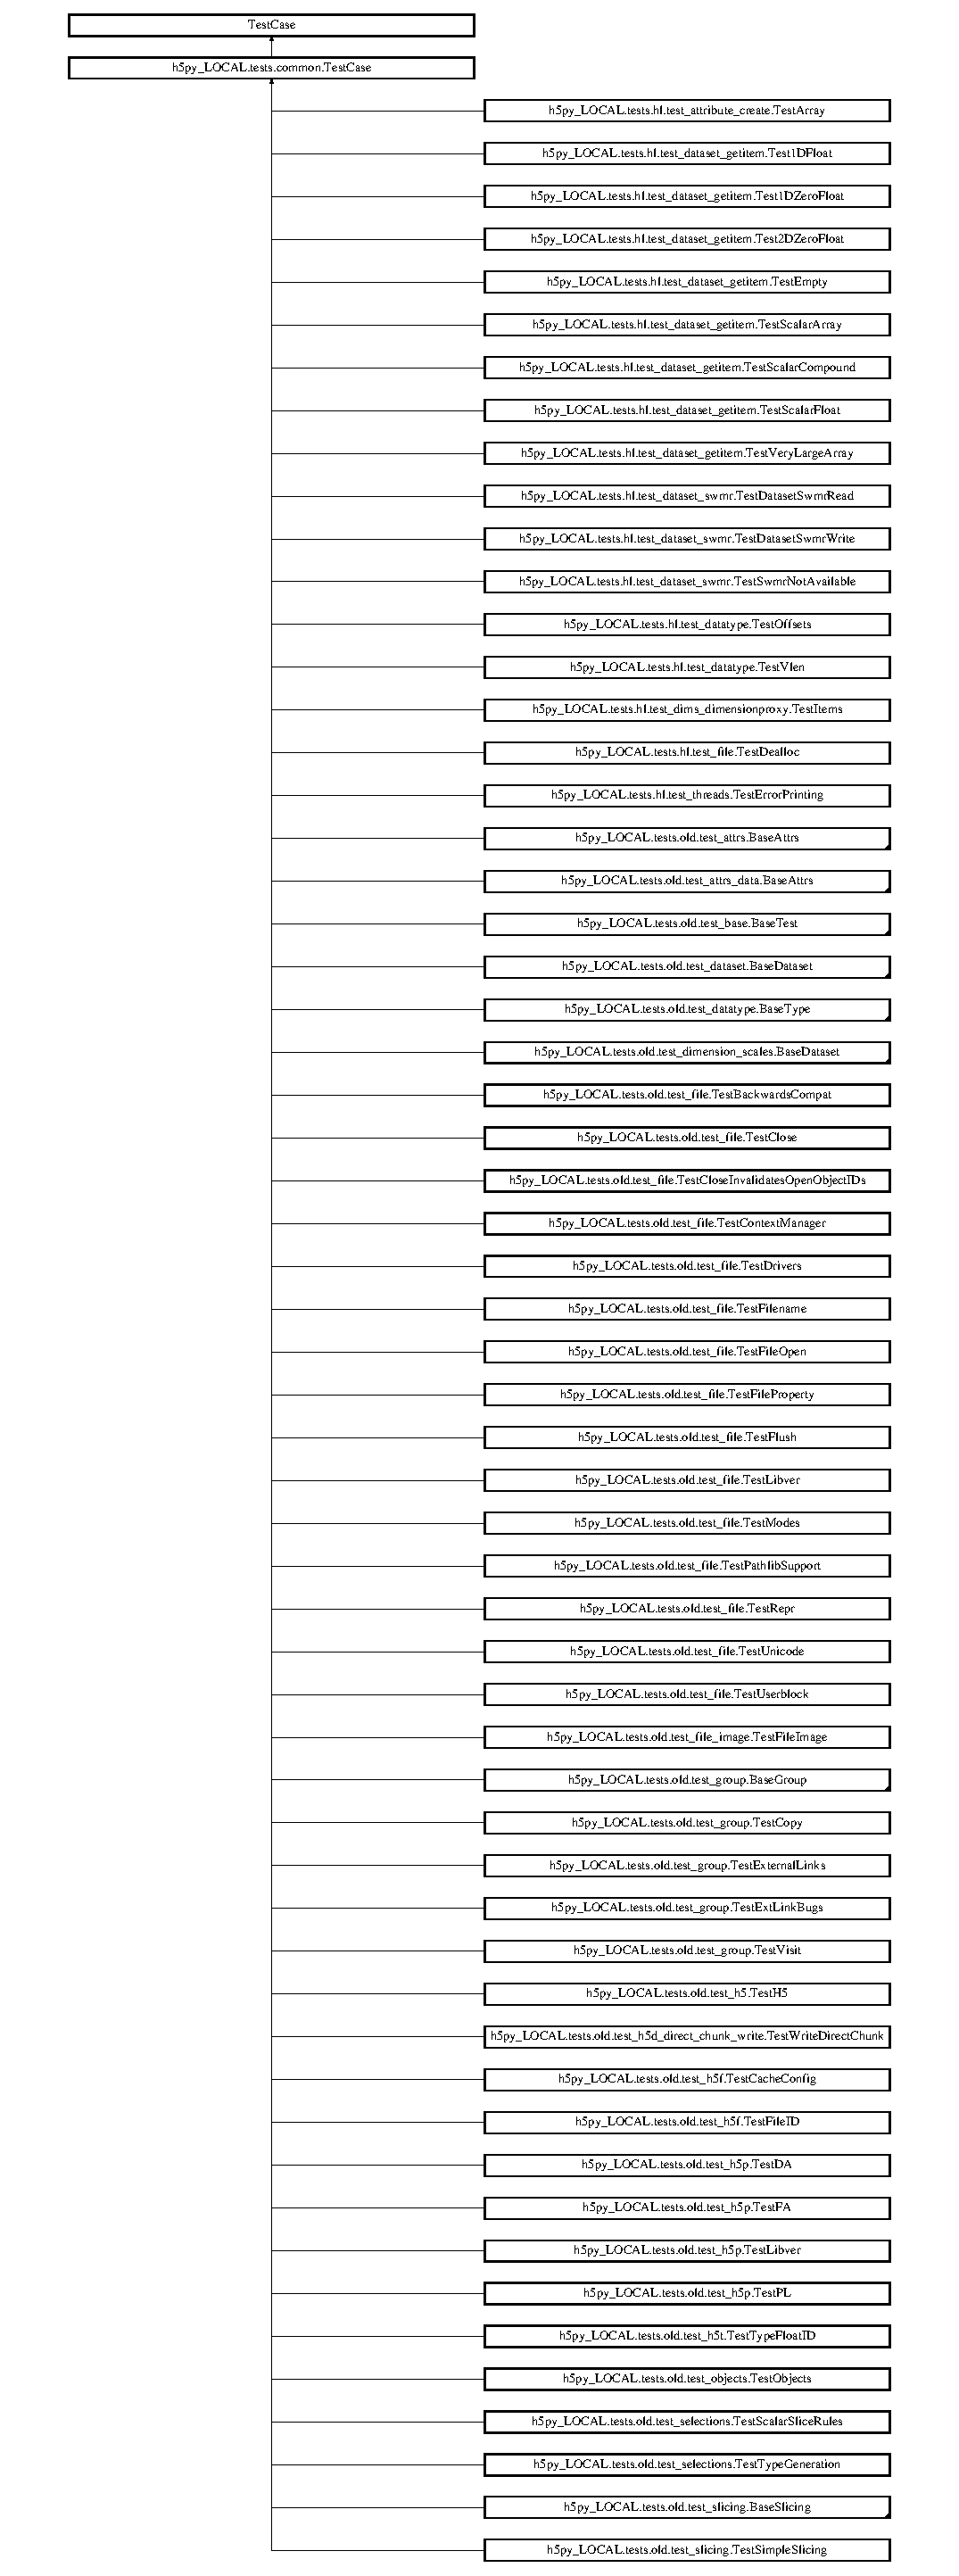
\includegraphics[height=12.000000cm]{classh5py__LOCAL_1_1tests_1_1common_1_1TestCase}
\end{center}
\end{figure}
\subsection*{Public Member Functions}
\begin{DoxyCompactItemize}
\item 
\mbox{\Hypertarget{classh5py__LOCAL_1_1tests_1_1common_1_1TestCase_adc65f7e8c0b14b2e7cc39c02c2522e8c}\label{classh5py__LOCAL_1_1tests_1_1common_1_1TestCase_adc65f7e8c0b14b2e7cc39c02c2522e8c}} 
def {\bfseries set\+Up\+Class} (cls)
\item 
\mbox{\Hypertarget{classh5py__LOCAL_1_1tests_1_1common_1_1TestCase_ad68b227379041a73f8045888a3147b97}\label{classh5py__LOCAL_1_1tests_1_1common_1_1TestCase_ad68b227379041a73f8045888a3147b97}} 
def {\bfseries tear\+Down\+Class} (cls)
\item 
\mbox{\Hypertarget{classh5py__LOCAL_1_1tests_1_1common_1_1TestCase_a849e16e410c6000e9e6f906602bebfb4}\label{classh5py__LOCAL_1_1tests_1_1common_1_1TestCase_a849e16e410c6000e9e6f906602bebfb4}} 
def {\bfseries mktemp} (self, suffix=\textquotesingle{}.hdf5\textquotesingle{}, prefix=\textquotesingle{}\textquotesingle{}, dir=None)
\item 
\mbox{\Hypertarget{classh5py__LOCAL_1_1tests_1_1common_1_1TestCase_ab16cdff0f0c625171b143a5595337374}\label{classh5py__LOCAL_1_1tests_1_1common_1_1TestCase_ab16cdff0f0c625171b143a5595337374}} 
def {\bfseries set\+Up} (self)
\item 
\mbox{\Hypertarget{classh5py__LOCAL_1_1tests_1_1common_1_1TestCase_a975cd319f3a70020a969ad6690ea791b}\label{classh5py__LOCAL_1_1tests_1_1common_1_1TestCase_a975cd319f3a70020a969ad6690ea791b}} 
def {\bfseries tear\+Down} (self)
\item 
\mbox{\Hypertarget{classh5py__LOCAL_1_1tests_1_1common_1_1TestCase_aa7438679aa3773de8fda4f8e84435007}\label{classh5py__LOCAL_1_1tests_1_1common_1_1TestCase_aa7438679aa3773de8fda4f8e84435007}} 
def {\bfseries assert\+Same\+Elements} (self, a, b)
\item 
def \hyperlink{classh5py__LOCAL_1_1tests_1_1common_1_1TestCase_a4048c84ae90d454d0545ca1def1f4326}{assert\+Array\+Equal} (self, dset, arr, message=None, precision=None)
\item 
def \hyperlink{classh5py__LOCAL_1_1tests_1_1common_1_1TestCase_aae2a888455d3593a87623e41e0a838a7}{assert\+Numpy\+Behavior} (self, dset, arr, s)
\end{DoxyCompactItemize}
\subsection*{Public Attributes}
\begin{DoxyCompactItemize}
\item 
\mbox{\Hypertarget{classh5py__LOCAL_1_1tests_1_1common_1_1TestCase_a3097303391ce019c15238e5223dc39fe}\label{classh5py__LOCAL_1_1tests_1_1common_1_1TestCase_a3097303391ce019c15238e5223dc39fe}} 
{\bfseries tempdir}
\item 
\mbox{\Hypertarget{classh5py__LOCAL_1_1tests_1_1common_1_1TestCase_a871b4536ef7c8908a995f4ea924325c7}\label{classh5py__LOCAL_1_1tests_1_1common_1_1TestCase_a871b4536ef7c8908a995f4ea924325c7}} 
{\bfseries f}
\end{DoxyCompactItemize}


\subsection{Detailed Description}
\begin{DoxyVerb}    Base class for unit tests.
\end{DoxyVerb}
 

\subsection{Member Function Documentation}
\mbox{\Hypertarget{classh5py__LOCAL_1_1tests_1_1common_1_1TestCase_a4048c84ae90d454d0545ca1def1f4326}\label{classh5py__LOCAL_1_1tests_1_1common_1_1TestCase_a4048c84ae90d454d0545ca1def1f4326}} 
\index{h5py\+\_\+\+L\+O\+C\+A\+L\+::tests\+::common\+::\+Test\+Case@{h5py\+\_\+\+L\+O\+C\+A\+L\+::tests\+::common\+::\+Test\+Case}!assert\+Array\+Equal@{assert\+Array\+Equal}}
\index{assert\+Array\+Equal@{assert\+Array\+Equal}!h5py\+\_\+\+L\+O\+C\+A\+L\+::tests\+::common\+::\+Test\+Case@{h5py\+\_\+\+L\+O\+C\+A\+L\+::tests\+::common\+::\+Test\+Case}}
\subsubsection{\texorpdfstring{assert\+Array\+Equal()}{assertArrayEqual()}}
{\footnotesize\ttfamily def h5py\+\_\+\+L\+O\+C\+A\+L.\+tests.\+common.\+Test\+Case.\+assert\+Array\+Equal (\begin{DoxyParamCaption}\item[{}]{self,  }\item[{}]{dset,  }\item[{}]{arr,  }\item[{}]{message = {\ttfamily None},  }\item[{}]{precision = {\ttfamily None} }\end{DoxyParamCaption})}

\begin{DoxyVerb}Make sure dset and arr have the same shape, dtype and contents, to
    within the given precision.

    Note that dset may be a NumPy array or an HDF5 dataset.
\end{DoxyVerb}
 \mbox{\Hypertarget{classh5py__LOCAL_1_1tests_1_1common_1_1TestCase_aae2a888455d3593a87623e41e0a838a7}\label{classh5py__LOCAL_1_1tests_1_1common_1_1TestCase_aae2a888455d3593a87623e41e0a838a7}} 
\index{h5py\+\_\+\+L\+O\+C\+A\+L\+::tests\+::common\+::\+Test\+Case@{h5py\+\_\+\+L\+O\+C\+A\+L\+::tests\+::common\+::\+Test\+Case}!assert\+Numpy\+Behavior@{assert\+Numpy\+Behavior}}
\index{assert\+Numpy\+Behavior@{assert\+Numpy\+Behavior}!h5py\+\_\+\+L\+O\+C\+A\+L\+::tests\+::common\+::\+Test\+Case@{h5py\+\_\+\+L\+O\+C\+A\+L\+::tests\+::common\+::\+Test\+Case}}
\subsubsection{\texorpdfstring{assert\+Numpy\+Behavior()}{assertNumpyBehavior()}}
{\footnotesize\ttfamily def h5py\+\_\+\+L\+O\+C\+A\+L.\+tests.\+common.\+Test\+Case.\+assert\+Numpy\+Behavior (\begin{DoxyParamCaption}\item[{}]{self,  }\item[{}]{dset,  }\item[{}]{arr,  }\item[{}]{s }\end{DoxyParamCaption})}

\begin{DoxyVerb}Apply slicing arguments "s" to both dset and arr.

Succeeds if the results of the slicing are identical, or the
exception raised is of the same type for both.

"arr" must be a Numpy array; "dset" may be a NumPy array or dataset.
\end{DoxyVerb}
 

The documentation for this class was generated from the following file\+:\begin{DoxyCompactItemize}
\item 
src/mesh\+\_\+formats/hdf/h5py\+\_\+\+L\+O\+C\+A\+L/tests/common.\+py\end{DoxyCompactItemize}

\hypertarget{classh5py__LOCAL_1_1tests_1_1old_1_1test__file_1_1TestClose}{}\section{h5py\+\_\+\+L\+O\+C\+A\+L.\+tests.\+old.\+test\+\_\+file.\+Test\+Close Class Reference}
\label{classh5py__LOCAL_1_1tests_1_1old_1_1test__file_1_1TestClose}\index{h5py\+\_\+\+L\+O\+C\+A\+L.\+tests.\+old.\+test\+\_\+file.\+Test\+Close@{h5py\+\_\+\+L\+O\+C\+A\+L.\+tests.\+old.\+test\+\_\+file.\+Test\+Close}}
Inheritance diagram for h5py\+\_\+\+L\+O\+C\+A\+L.\+tests.\+old.\+test\+\_\+file.\+Test\+Close\+:\begin{figure}[H]
\begin{center}
\leavevmode
\includegraphics[height=3.000000cm]{classh5py__LOCAL_1_1tests_1_1old_1_1test__file_1_1TestClose}
\end{center}
\end{figure}
\subsection*{Public Member Functions}
\begin{DoxyCompactItemize}
\item 
def \hyperlink{classh5py__LOCAL_1_1tests_1_1old_1_1test__file_1_1TestClose_ae609f084d70fb53adf37a6224f40e90f}{test\+\_\+close} (self)
\item 
def \hyperlink{classh5py__LOCAL_1_1tests_1_1old_1_1test__file_1_1TestClose_a17a9ad9f2ce4f4d285fb2c0c91b721a2}{test\+\_\+closed\+\_\+file} (self)
\item 
\mbox{\Hypertarget{classh5py__LOCAL_1_1tests_1_1old_1_1test__file_1_1TestClose_ae313aafce6f3007f58d8f756aa18bf58}\label{classh5py__LOCAL_1_1tests_1_1old_1_1test__file_1_1TestClose_ae313aafce6f3007f58d8f756aa18bf58}} 
def {\bfseries test\+\_\+close\+\_\+multiple\+\_\+default\+\_\+driver} (self)
\item 
def \hyperlink{classh5py__LOCAL_1_1tests_1_1old_1_1test__file_1_1TestClose_a2a4f3b4c75399922b2db2793a450214d}{test\+\_\+close\+\_\+multiple\+\_\+mpio\+\_\+driver} (self)
\end{DoxyCompactItemize}
\subsection*{Additional Inherited Members}


\subsection{Detailed Description}
\begin{DoxyVerb}    Feature: Files can be closed
\end{DoxyVerb}
 

\subsection{Member Function Documentation}
\mbox{\Hypertarget{classh5py__LOCAL_1_1tests_1_1old_1_1test__file_1_1TestClose_ae609f084d70fb53adf37a6224f40e90f}\label{classh5py__LOCAL_1_1tests_1_1old_1_1test__file_1_1TestClose_ae609f084d70fb53adf37a6224f40e90f}} 
\index{h5py\+\_\+\+L\+O\+C\+A\+L\+::tests\+::old\+::test\+\_\+file\+::\+Test\+Close@{h5py\+\_\+\+L\+O\+C\+A\+L\+::tests\+::old\+::test\+\_\+file\+::\+Test\+Close}!test\+\_\+close@{test\+\_\+close}}
\index{test\+\_\+close@{test\+\_\+close}!h5py\+\_\+\+L\+O\+C\+A\+L\+::tests\+::old\+::test\+\_\+file\+::\+Test\+Close@{h5py\+\_\+\+L\+O\+C\+A\+L\+::tests\+::old\+::test\+\_\+file\+::\+Test\+Close}}
\subsubsection{\texorpdfstring{test\+\_\+close()}{test\_close()}}
{\footnotesize\ttfamily def h5py\+\_\+\+L\+O\+C\+A\+L.\+tests.\+old.\+test\+\_\+file.\+Test\+Close.\+test\+\_\+close (\begin{DoxyParamCaption}\item[{}]{self }\end{DoxyParamCaption})}

\begin{DoxyVerb}Close file via .close method \end{DoxyVerb}
 \mbox{\Hypertarget{classh5py__LOCAL_1_1tests_1_1old_1_1test__file_1_1TestClose_a2a4f3b4c75399922b2db2793a450214d}\label{classh5py__LOCAL_1_1tests_1_1old_1_1test__file_1_1TestClose_a2a4f3b4c75399922b2db2793a450214d}} 
\index{h5py\+\_\+\+L\+O\+C\+A\+L\+::tests\+::old\+::test\+\_\+file\+::\+Test\+Close@{h5py\+\_\+\+L\+O\+C\+A\+L\+::tests\+::old\+::test\+\_\+file\+::\+Test\+Close}!test\+\_\+close\+\_\+multiple\+\_\+mpio\+\_\+driver@{test\+\_\+close\+\_\+multiple\+\_\+mpio\+\_\+driver}}
\index{test\+\_\+close\+\_\+multiple\+\_\+mpio\+\_\+driver@{test\+\_\+close\+\_\+multiple\+\_\+mpio\+\_\+driver}!h5py\+\_\+\+L\+O\+C\+A\+L\+::tests\+::old\+::test\+\_\+file\+::\+Test\+Close@{h5py\+\_\+\+L\+O\+C\+A\+L\+::tests\+::old\+::test\+\_\+file\+::\+Test\+Close}}
\subsubsection{\texorpdfstring{test\+\_\+close\+\_\+multiple\+\_\+mpio\+\_\+driver()}{test\_close\_multiple\_mpio\_driver()}}
{\footnotesize\ttfamily def h5py\+\_\+\+L\+O\+C\+A\+L.\+tests.\+old.\+test\+\_\+file.\+Test\+Close.\+test\+\_\+close\+\_\+multiple\+\_\+mpio\+\_\+driver (\begin{DoxyParamCaption}\item[{}]{self }\end{DoxyParamCaption})}

\begin{DoxyVerb}MPIO driver and options \end{DoxyVerb}
 \mbox{\Hypertarget{classh5py__LOCAL_1_1tests_1_1old_1_1test__file_1_1TestClose_a17a9ad9f2ce4f4d285fb2c0c91b721a2}\label{classh5py__LOCAL_1_1tests_1_1old_1_1test__file_1_1TestClose_a17a9ad9f2ce4f4d285fb2c0c91b721a2}} 
\index{h5py\+\_\+\+L\+O\+C\+A\+L\+::tests\+::old\+::test\+\_\+file\+::\+Test\+Close@{h5py\+\_\+\+L\+O\+C\+A\+L\+::tests\+::old\+::test\+\_\+file\+::\+Test\+Close}!test\+\_\+closed\+\_\+file@{test\+\_\+closed\+\_\+file}}
\index{test\+\_\+closed\+\_\+file@{test\+\_\+closed\+\_\+file}!h5py\+\_\+\+L\+O\+C\+A\+L\+::tests\+::old\+::test\+\_\+file\+::\+Test\+Close@{h5py\+\_\+\+L\+O\+C\+A\+L\+::tests\+::old\+::test\+\_\+file\+::\+Test\+Close}}
\subsubsection{\texorpdfstring{test\+\_\+closed\+\_\+file()}{test\_closed\_file()}}
{\footnotesize\ttfamily def h5py\+\_\+\+L\+O\+C\+A\+L.\+tests.\+old.\+test\+\_\+file.\+Test\+Close.\+test\+\_\+closed\+\_\+file (\begin{DoxyParamCaption}\item[{}]{self }\end{DoxyParamCaption})}

\begin{DoxyVerb}Trying to modify closed file raises ValueError \end{DoxyVerb}
 

The documentation for this class was generated from the following file\+:\begin{DoxyCompactItemize}
\item 
src/mesh\+\_\+formats/hdf/h5py\+\_\+\+L\+O\+C\+A\+L/tests/old/test\+\_\+file.\+py\end{DoxyCompactItemize}

\hypertarget{classh5py__LOCAL_1_1tests_1_1old_1_1test__file_1_1TestCloseInvalidatesOpenObjectIDs}{}\section{h5py\+\_\+\+L\+O\+C\+A\+L.\+tests.\+old.\+test\+\_\+file.\+Test\+Close\+Invalidates\+Open\+Object\+I\+Ds Class Reference}
\label{classh5py__LOCAL_1_1tests_1_1old_1_1test__file_1_1TestCloseInvalidatesOpenObjectIDs}\index{h5py\+\_\+\+L\+O\+C\+A\+L.\+tests.\+old.\+test\+\_\+file.\+Test\+Close\+Invalidates\+Open\+Object\+I\+Ds@{h5py\+\_\+\+L\+O\+C\+A\+L.\+tests.\+old.\+test\+\_\+file.\+Test\+Close\+Invalidates\+Open\+Object\+I\+Ds}}
Inheritance diagram for h5py\+\_\+\+L\+O\+C\+A\+L.\+tests.\+old.\+test\+\_\+file.\+Test\+Close\+Invalidates\+Open\+Object\+I\+Ds\+:\begin{figure}[H]
\begin{center}
\leavevmode
\includegraphics[height=3.000000cm]{classh5py__LOCAL_1_1tests_1_1old_1_1test__file_1_1TestCloseInvalidatesOpenObjectIDs}
\end{center}
\end{figure}
\subsection*{Public Member Functions}
\begin{DoxyCompactItemize}
\item 
def \hyperlink{classh5py__LOCAL_1_1tests_1_1old_1_1test__file_1_1TestCloseInvalidatesOpenObjectIDs_a3ba05b53d0fcc1246b4f2235ececec79}{test\+\_\+close} (self)
\end{DoxyCompactItemize}
\subsection*{Additional Inherited Members}


\subsection{Detailed Description}
\begin{DoxyVerb}    Ensure that closing a file invalidates object IDs, as appropriate
\end{DoxyVerb}
 

\subsection{Member Function Documentation}
\mbox{\Hypertarget{classh5py__LOCAL_1_1tests_1_1old_1_1test__file_1_1TestCloseInvalidatesOpenObjectIDs_a3ba05b53d0fcc1246b4f2235ececec79}\label{classh5py__LOCAL_1_1tests_1_1old_1_1test__file_1_1TestCloseInvalidatesOpenObjectIDs_a3ba05b53d0fcc1246b4f2235ececec79}} 
\index{h5py\+\_\+\+L\+O\+C\+A\+L\+::tests\+::old\+::test\+\_\+file\+::\+Test\+Close\+Invalidates\+Open\+Object\+I\+Ds@{h5py\+\_\+\+L\+O\+C\+A\+L\+::tests\+::old\+::test\+\_\+file\+::\+Test\+Close\+Invalidates\+Open\+Object\+I\+Ds}!test\+\_\+close@{test\+\_\+close}}
\index{test\+\_\+close@{test\+\_\+close}!h5py\+\_\+\+L\+O\+C\+A\+L\+::tests\+::old\+::test\+\_\+file\+::\+Test\+Close\+Invalidates\+Open\+Object\+I\+Ds@{h5py\+\_\+\+L\+O\+C\+A\+L\+::tests\+::old\+::test\+\_\+file\+::\+Test\+Close\+Invalidates\+Open\+Object\+I\+Ds}}
\subsubsection{\texorpdfstring{test\+\_\+close()}{test\_close()}}
{\footnotesize\ttfamily def h5py\+\_\+\+L\+O\+C\+A\+L.\+tests.\+old.\+test\+\_\+file.\+Test\+Close\+Invalidates\+Open\+Object\+I\+Ds.\+test\+\_\+close (\begin{DoxyParamCaption}\item[{}]{self }\end{DoxyParamCaption})}

\begin{DoxyVerb}Closing a file invalidates any of the file's open objects \end{DoxyVerb}
 

The documentation for this class was generated from the following file\+:\begin{DoxyCompactItemize}
\item 
src/mesh\+\_\+formats/hdf/h5py\+\_\+\+L\+O\+C\+A\+L/tests/old/test\+\_\+file.\+py\end{DoxyCompactItemize}

\hypertarget{classh5py__LOCAL_1_1tests_1_1old_1_1test__h5t_1_1TestCompound}{}\section{h5py\+\_\+\+L\+O\+C\+A\+L.\+tests.\+old.\+test\+\_\+h5t.\+Test\+Compound Class Reference}
\label{classh5py__LOCAL_1_1tests_1_1old_1_1test__h5t_1_1TestCompound}\index{h5py\+\_\+\+L\+O\+C\+A\+L.\+tests.\+old.\+test\+\_\+h5t.\+Test\+Compound@{h5py\+\_\+\+L\+O\+C\+A\+L.\+tests.\+old.\+test\+\_\+h5t.\+Test\+Compound}}
Inheritance diagram for h5py\+\_\+\+L\+O\+C\+A\+L.\+tests.\+old.\+test\+\_\+h5t.\+Test\+Compound\+:\begin{figure}[H]
\begin{center}
\leavevmode
\includegraphics[height=2.000000cm]{classh5py__LOCAL_1_1tests_1_1old_1_1test__h5t_1_1TestCompound}
\end{center}
\end{figure}
\subsection*{Public Member Functions}
\begin{DoxyCompactItemize}
\item 
def \hyperlink{classh5py__LOCAL_1_1tests_1_1old_1_1test__h5t_1_1TestCompound_a270d282e47a4a0cfc96a9ad5209bb74e}{test\+\_\+ref} (self)
\item 
\mbox{\Hypertarget{classh5py__LOCAL_1_1tests_1_1old_1_1test__h5t_1_1TestCompound_a484cdc483dc095e78dc2bd41c37c6f3b}\label{classh5py__LOCAL_1_1tests_1_1old_1_1test__h5t_1_1TestCompound_a484cdc483dc095e78dc2bd41c37c6f3b}} 
def {\bfseries test\+\_\+out\+\_\+of\+\_\+order\+\_\+offsets} (self)
\end{DoxyCompactItemize}


\subsection{Detailed Description}
\begin{DoxyVerb}    Feature: Compound types can be created from Python dtypes
\end{DoxyVerb}
 

\subsection{Member Function Documentation}
\mbox{\Hypertarget{classh5py__LOCAL_1_1tests_1_1old_1_1test__h5t_1_1TestCompound_a270d282e47a4a0cfc96a9ad5209bb74e}\label{classh5py__LOCAL_1_1tests_1_1old_1_1test__h5t_1_1TestCompound_a270d282e47a4a0cfc96a9ad5209bb74e}} 
\index{h5py\+\_\+\+L\+O\+C\+A\+L\+::tests\+::old\+::test\+\_\+h5t\+::\+Test\+Compound@{h5py\+\_\+\+L\+O\+C\+A\+L\+::tests\+::old\+::test\+\_\+h5t\+::\+Test\+Compound}!test\+\_\+ref@{test\+\_\+ref}}
\index{test\+\_\+ref@{test\+\_\+ref}!h5py\+\_\+\+L\+O\+C\+A\+L\+::tests\+::old\+::test\+\_\+h5t\+::\+Test\+Compound@{h5py\+\_\+\+L\+O\+C\+A\+L\+::tests\+::old\+::test\+\_\+h5t\+::\+Test\+Compound}}
\subsubsection{\texorpdfstring{test\+\_\+ref()}{test\_ref()}}
{\footnotesize\ttfamily def h5py\+\_\+\+L\+O\+C\+A\+L.\+tests.\+old.\+test\+\_\+h5t.\+Test\+Compound.\+test\+\_\+ref (\begin{DoxyParamCaption}\item[{}]{self }\end{DoxyParamCaption})}

\begin{DoxyVerb}Reference types are correctly stored in compound types (issue 144)
\end{DoxyVerb}
 

The documentation for this class was generated from the following file\+:\begin{DoxyCompactItemize}
\item 
src/mesh\+\_\+formats/hdf/h5py\+\_\+\+L\+O\+C\+A\+L/tests/old/test\+\_\+h5t.\+py\end{DoxyCompactItemize}

\hypertarget{classh5py__LOCAL_1_1tests_1_1old_1_1test__dataset_1_1TestCompound}{}\section{h5py\+\_\+\+L\+O\+C\+A\+L.\+tests.\+old.\+test\+\_\+dataset.\+Test\+Compound Class Reference}
\label{classh5py__LOCAL_1_1tests_1_1old_1_1test__dataset_1_1TestCompound}\index{h5py\+\_\+\+L\+O\+C\+A\+L.\+tests.\+old.\+test\+\_\+dataset.\+Test\+Compound@{h5py\+\_\+\+L\+O\+C\+A\+L.\+tests.\+old.\+test\+\_\+dataset.\+Test\+Compound}}
Inheritance diagram for h5py\+\_\+\+L\+O\+C\+A\+L.\+tests.\+old.\+test\+\_\+dataset.\+Test\+Compound\+:\begin{figure}[H]
\begin{center}
\leavevmode
\includegraphics[height=4.000000cm]{classh5py__LOCAL_1_1tests_1_1old_1_1test__dataset_1_1TestCompound}
\end{center}
\end{figure}
\subsection*{Public Member Functions}
\begin{DoxyCompactItemize}
\item 
def \hyperlink{classh5py__LOCAL_1_1tests_1_1old_1_1test__dataset_1_1TestCompound_a47d6c406ac4def451ba8d75a3efff3e9}{test\+\_\+rt} (self)
\item 
\mbox{\Hypertarget{classh5py__LOCAL_1_1tests_1_1old_1_1test__dataset_1_1TestCompound_a3fab381c192e03b43419737ebd615fad}\label{classh5py__LOCAL_1_1tests_1_1old_1_1test__dataset_1_1TestCompound_a3fab381c192e03b43419737ebd615fad}} 
def {\bfseries test\+\_\+assign} (self)
\end{DoxyCompactItemize}
\subsection*{Additional Inherited Members}


\subsection{Detailed Description}
\begin{DoxyVerb}    Feature: Compound types correctly round-trip
\end{DoxyVerb}
 

\subsection{Member Function Documentation}
\mbox{\Hypertarget{classh5py__LOCAL_1_1tests_1_1old_1_1test__dataset_1_1TestCompound_a47d6c406ac4def451ba8d75a3efff3e9}\label{classh5py__LOCAL_1_1tests_1_1old_1_1test__dataset_1_1TestCompound_a47d6c406ac4def451ba8d75a3efff3e9}} 
\index{h5py\+\_\+\+L\+O\+C\+A\+L\+::tests\+::old\+::test\+\_\+dataset\+::\+Test\+Compound@{h5py\+\_\+\+L\+O\+C\+A\+L\+::tests\+::old\+::test\+\_\+dataset\+::\+Test\+Compound}!test\+\_\+rt@{test\+\_\+rt}}
\index{test\+\_\+rt@{test\+\_\+rt}!h5py\+\_\+\+L\+O\+C\+A\+L\+::tests\+::old\+::test\+\_\+dataset\+::\+Test\+Compound@{h5py\+\_\+\+L\+O\+C\+A\+L\+::tests\+::old\+::test\+\_\+dataset\+::\+Test\+Compound}}
\subsubsection{\texorpdfstring{test\+\_\+rt()}{test\_rt()}}
{\footnotesize\ttfamily def h5py\+\_\+\+L\+O\+C\+A\+L.\+tests.\+old.\+test\+\_\+dataset.\+Test\+Compound.\+test\+\_\+rt (\begin{DoxyParamCaption}\item[{}]{self }\end{DoxyParamCaption})}

\begin{DoxyVerb}Compound types are read back in correct order (issue 236)\end{DoxyVerb}
 

The documentation for this class was generated from the following file\+:\begin{DoxyCompactItemize}
\item 
src/mesh\+\_\+formats/hdf/h5py\+\_\+\+L\+O\+C\+A\+L/tests/old/test\+\_\+dataset.\+py\end{DoxyCompactItemize}

\hypertarget{classh5py__LOCAL_1_1tests_1_1old_1_1test__group_1_1TestContains}{}\section{h5py\+\_\+\+L\+O\+C\+A\+L.\+tests.\+old.\+test\+\_\+group.\+Test\+Contains Class Reference}
\label{classh5py__LOCAL_1_1tests_1_1old_1_1test__group_1_1TestContains}\index{h5py\+\_\+\+L\+O\+C\+A\+L.\+tests.\+old.\+test\+\_\+group.\+Test\+Contains@{h5py\+\_\+\+L\+O\+C\+A\+L.\+tests.\+old.\+test\+\_\+group.\+Test\+Contains}}
Inheritance diagram for h5py\+\_\+\+L\+O\+C\+A\+L.\+tests.\+old.\+test\+\_\+group.\+Test\+Contains\+:\begin{figure}[H]
\begin{center}
\leavevmode
\includegraphics[height=4.000000cm]{classh5py__LOCAL_1_1tests_1_1old_1_1test__group_1_1TestContains}
\end{center}
\end{figure}
\subsection*{Public Member Functions}
\begin{DoxyCompactItemize}
\item 
def \hyperlink{classh5py__LOCAL_1_1tests_1_1old_1_1test__group_1_1TestContains_a3c86bef8d26cbb2a7768aa559e1d3218}{test\+\_\+contains} (self)
\item 
def \hyperlink{classh5py__LOCAL_1_1tests_1_1old_1_1test__group_1_1TestContains_a040d470e31150644a8c853d02d3d06e6}{test\+\_\+exc} (self)
\item 
def \hyperlink{classh5py__LOCAL_1_1tests_1_1old_1_1test__group_1_1TestContains_a964bb18d3467e0642a15b7853bf13a02}{test\+\_\+empty} (self)
\item 
def \hyperlink{classh5py__LOCAL_1_1tests_1_1old_1_1test__group_1_1TestContains_a66d49920420aad01f4806afcbe3b97bf}{test\+\_\+dot} (self)
\item 
def \hyperlink{classh5py__LOCAL_1_1tests_1_1old_1_1test__group_1_1TestContains_aafa5cee29fe97a5b2364c9c37140ae93}{test\+\_\+root} (self)
\item 
def \hyperlink{classh5py__LOCAL_1_1tests_1_1old_1_1test__group_1_1TestContains_a5871689c1aecf06ce4b529e72b634d33}{test\+\_\+trailing\+\_\+slash} (self)
\item 
def \hyperlink{classh5py__LOCAL_1_1tests_1_1old_1_1test__group_1_1TestContains_ace6cb7c30b6f49ddede373edb79a3dc3}{test\+\_\+softlinks} (self)
\item 
def \hyperlink{classh5py__LOCAL_1_1tests_1_1old_1_1test__group_1_1TestContains_aeb321e29d89f919242903daec3815630}{test\+\_\+oddball\+\_\+paths} (self)
\end{DoxyCompactItemize}
\subsection*{Additional Inherited Members}


\subsection{Detailed Description}
\begin{DoxyVerb}    Feature: The Python "in" builtin tests for membership
\end{DoxyVerb}
 

\subsection{Member Function Documentation}
\mbox{\Hypertarget{classh5py__LOCAL_1_1tests_1_1old_1_1test__group_1_1TestContains_a3c86bef8d26cbb2a7768aa559e1d3218}\label{classh5py__LOCAL_1_1tests_1_1old_1_1test__group_1_1TestContains_a3c86bef8d26cbb2a7768aa559e1d3218}} 
\index{h5py\+\_\+\+L\+O\+C\+A\+L\+::tests\+::old\+::test\+\_\+group\+::\+Test\+Contains@{h5py\+\_\+\+L\+O\+C\+A\+L\+::tests\+::old\+::test\+\_\+group\+::\+Test\+Contains}!test\+\_\+contains@{test\+\_\+contains}}
\index{test\+\_\+contains@{test\+\_\+contains}!h5py\+\_\+\+L\+O\+C\+A\+L\+::tests\+::old\+::test\+\_\+group\+::\+Test\+Contains@{h5py\+\_\+\+L\+O\+C\+A\+L\+::tests\+::old\+::test\+\_\+group\+::\+Test\+Contains}}
\subsubsection{\texorpdfstring{test\+\_\+contains()}{test\_contains()}}
{\footnotesize\ttfamily def h5py\+\_\+\+L\+O\+C\+A\+L.\+tests.\+old.\+test\+\_\+group.\+Test\+Contains.\+test\+\_\+contains (\begin{DoxyParamCaption}\item[{}]{self }\end{DoxyParamCaption})}

\begin{DoxyVerb}"in" builtin works for membership (byte and Unicode) \end{DoxyVerb}
 \mbox{\Hypertarget{classh5py__LOCAL_1_1tests_1_1old_1_1test__group_1_1TestContains_a66d49920420aad01f4806afcbe3b97bf}\label{classh5py__LOCAL_1_1tests_1_1old_1_1test__group_1_1TestContains_a66d49920420aad01f4806afcbe3b97bf}} 
\index{h5py\+\_\+\+L\+O\+C\+A\+L\+::tests\+::old\+::test\+\_\+group\+::\+Test\+Contains@{h5py\+\_\+\+L\+O\+C\+A\+L\+::tests\+::old\+::test\+\_\+group\+::\+Test\+Contains}!test\+\_\+dot@{test\+\_\+dot}}
\index{test\+\_\+dot@{test\+\_\+dot}!h5py\+\_\+\+L\+O\+C\+A\+L\+::tests\+::old\+::test\+\_\+group\+::\+Test\+Contains@{h5py\+\_\+\+L\+O\+C\+A\+L\+::tests\+::old\+::test\+\_\+group\+::\+Test\+Contains}}
\subsubsection{\texorpdfstring{test\+\_\+dot()}{test\_dot()}}
{\footnotesize\ttfamily def h5py\+\_\+\+L\+O\+C\+A\+L.\+tests.\+old.\+test\+\_\+group.\+Test\+Contains.\+test\+\_\+dot (\begin{DoxyParamCaption}\item[{}]{self }\end{DoxyParamCaption})}

\begin{DoxyVerb}Current group "." is always contained \end{DoxyVerb}
 \mbox{\Hypertarget{classh5py__LOCAL_1_1tests_1_1old_1_1test__group_1_1TestContains_a964bb18d3467e0642a15b7853bf13a02}\label{classh5py__LOCAL_1_1tests_1_1old_1_1test__group_1_1TestContains_a964bb18d3467e0642a15b7853bf13a02}} 
\index{h5py\+\_\+\+L\+O\+C\+A\+L\+::tests\+::old\+::test\+\_\+group\+::\+Test\+Contains@{h5py\+\_\+\+L\+O\+C\+A\+L\+::tests\+::old\+::test\+\_\+group\+::\+Test\+Contains}!test\+\_\+empty@{test\+\_\+empty}}
\index{test\+\_\+empty@{test\+\_\+empty}!h5py\+\_\+\+L\+O\+C\+A\+L\+::tests\+::old\+::test\+\_\+group\+::\+Test\+Contains@{h5py\+\_\+\+L\+O\+C\+A\+L\+::tests\+::old\+::test\+\_\+group\+::\+Test\+Contains}}
\subsubsection{\texorpdfstring{test\+\_\+empty()}{test\_empty()}}
{\footnotesize\ttfamily def h5py\+\_\+\+L\+O\+C\+A\+L.\+tests.\+old.\+test\+\_\+group.\+Test\+Contains.\+test\+\_\+empty (\begin{DoxyParamCaption}\item[{}]{self }\end{DoxyParamCaption})}

\begin{DoxyVerb}Empty strings work properly and aren't contained \end{DoxyVerb}
 \mbox{\Hypertarget{classh5py__LOCAL_1_1tests_1_1old_1_1test__group_1_1TestContains_a040d470e31150644a8c853d02d3d06e6}\label{classh5py__LOCAL_1_1tests_1_1old_1_1test__group_1_1TestContains_a040d470e31150644a8c853d02d3d06e6}} 
\index{h5py\+\_\+\+L\+O\+C\+A\+L\+::tests\+::old\+::test\+\_\+group\+::\+Test\+Contains@{h5py\+\_\+\+L\+O\+C\+A\+L\+::tests\+::old\+::test\+\_\+group\+::\+Test\+Contains}!test\+\_\+exc@{test\+\_\+exc}}
\index{test\+\_\+exc@{test\+\_\+exc}!h5py\+\_\+\+L\+O\+C\+A\+L\+::tests\+::old\+::test\+\_\+group\+::\+Test\+Contains@{h5py\+\_\+\+L\+O\+C\+A\+L\+::tests\+::old\+::test\+\_\+group\+::\+Test\+Contains}}
\subsubsection{\texorpdfstring{test\+\_\+exc()}{test\_exc()}}
{\footnotesize\ttfamily def h5py\+\_\+\+L\+O\+C\+A\+L.\+tests.\+old.\+test\+\_\+group.\+Test\+Contains.\+test\+\_\+exc (\begin{DoxyParamCaption}\item[{}]{self }\end{DoxyParamCaption})}

\begin{DoxyVerb}"in" on closed group returns False (see also issue 174) \end{DoxyVerb}
 \mbox{\Hypertarget{classh5py__LOCAL_1_1tests_1_1old_1_1test__group_1_1TestContains_aeb321e29d89f919242903daec3815630}\label{classh5py__LOCAL_1_1tests_1_1old_1_1test__group_1_1TestContains_aeb321e29d89f919242903daec3815630}} 
\index{h5py\+\_\+\+L\+O\+C\+A\+L\+::tests\+::old\+::test\+\_\+group\+::\+Test\+Contains@{h5py\+\_\+\+L\+O\+C\+A\+L\+::tests\+::old\+::test\+\_\+group\+::\+Test\+Contains}!test\+\_\+oddball\+\_\+paths@{test\+\_\+oddball\+\_\+paths}}
\index{test\+\_\+oddball\+\_\+paths@{test\+\_\+oddball\+\_\+paths}!h5py\+\_\+\+L\+O\+C\+A\+L\+::tests\+::old\+::test\+\_\+group\+::\+Test\+Contains@{h5py\+\_\+\+L\+O\+C\+A\+L\+::tests\+::old\+::test\+\_\+group\+::\+Test\+Contains}}
\subsubsection{\texorpdfstring{test\+\_\+oddball\+\_\+paths()}{test\_oddball\_paths()}}
{\footnotesize\ttfamily def h5py\+\_\+\+L\+O\+C\+A\+L.\+tests.\+old.\+test\+\_\+group.\+Test\+Contains.\+test\+\_\+oddball\+\_\+paths (\begin{DoxyParamCaption}\item[{}]{self }\end{DoxyParamCaption})}

\begin{DoxyVerb}Technically legitimate (but odd-looking) paths \end{DoxyVerb}
 \mbox{\Hypertarget{classh5py__LOCAL_1_1tests_1_1old_1_1test__group_1_1TestContains_aafa5cee29fe97a5b2364c9c37140ae93}\label{classh5py__LOCAL_1_1tests_1_1old_1_1test__group_1_1TestContains_aafa5cee29fe97a5b2364c9c37140ae93}} 
\index{h5py\+\_\+\+L\+O\+C\+A\+L\+::tests\+::old\+::test\+\_\+group\+::\+Test\+Contains@{h5py\+\_\+\+L\+O\+C\+A\+L\+::tests\+::old\+::test\+\_\+group\+::\+Test\+Contains}!test\+\_\+root@{test\+\_\+root}}
\index{test\+\_\+root@{test\+\_\+root}!h5py\+\_\+\+L\+O\+C\+A\+L\+::tests\+::old\+::test\+\_\+group\+::\+Test\+Contains@{h5py\+\_\+\+L\+O\+C\+A\+L\+::tests\+::old\+::test\+\_\+group\+::\+Test\+Contains}}
\subsubsection{\texorpdfstring{test\+\_\+root()}{test\_root()}}
{\footnotesize\ttfamily def h5py\+\_\+\+L\+O\+C\+A\+L.\+tests.\+old.\+test\+\_\+group.\+Test\+Contains.\+test\+\_\+root (\begin{DoxyParamCaption}\item[{}]{self }\end{DoxyParamCaption})}

\begin{DoxyVerb}Root group (by itself) is contained \end{DoxyVerb}
 \mbox{\Hypertarget{classh5py__LOCAL_1_1tests_1_1old_1_1test__group_1_1TestContains_ace6cb7c30b6f49ddede373edb79a3dc3}\label{classh5py__LOCAL_1_1tests_1_1old_1_1test__group_1_1TestContains_ace6cb7c30b6f49ddede373edb79a3dc3}} 
\index{h5py\+\_\+\+L\+O\+C\+A\+L\+::tests\+::old\+::test\+\_\+group\+::\+Test\+Contains@{h5py\+\_\+\+L\+O\+C\+A\+L\+::tests\+::old\+::test\+\_\+group\+::\+Test\+Contains}!test\+\_\+softlinks@{test\+\_\+softlinks}}
\index{test\+\_\+softlinks@{test\+\_\+softlinks}!h5py\+\_\+\+L\+O\+C\+A\+L\+::tests\+::old\+::test\+\_\+group\+::\+Test\+Contains@{h5py\+\_\+\+L\+O\+C\+A\+L\+::tests\+::old\+::test\+\_\+group\+::\+Test\+Contains}}
\subsubsection{\texorpdfstring{test\+\_\+softlinks()}{test\_softlinks()}}
{\footnotesize\ttfamily def h5py\+\_\+\+L\+O\+C\+A\+L.\+tests.\+old.\+test\+\_\+group.\+Test\+Contains.\+test\+\_\+softlinks (\begin{DoxyParamCaption}\item[{}]{self }\end{DoxyParamCaption})}

\begin{DoxyVerb}Broken softlinks are contained, but their members are not \end{DoxyVerb}
 \mbox{\Hypertarget{classh5py__LOCAL_1_1tests_1_1old_1_1test__group_1_1TestContains_a5871689c1aecf06ce4b529e72b634d33}\label{classh5py__LOCAL_1_1tests_1_1old_1_1test__group_1_1TestContains_a5871689c1aecf06ce4b529e72b634d33}} 
\index{h5py\+\_\+\+L\+O\+C\+A\+L\+::tests\+::old\+::test\+\_\+group\+::\+Test\+Contains@{h5py\+\_\+\+L\+O\+C\+A\+L\+::tests\+::old\+::test\+\_\+group\+::\+Test\+Contains}!test\+\_\+trailing\+\_\+slash@{test\+\_\+trailing\+\_\+slash}}
\index{test\+\_\+trailing\+\_\+slash@{test\+\_\+trailing\+\_\+slash}!h5py\+\_\+\+L\+O\+C\+A\+L\+::tests\+::old\+::test\+\_\+group\+::\+Test\+Contains@{h5py\+\_\+\+L\+O\+C\+A\+L\+::tests\+::old\+::test\+\_\+group\+::\+Test\+Contains}}
\subsubsection{\texorpdfstring{test\+\_\+trailing\+\_\+slash()}{test\_trailing\_slash()}}
{\footnotesize\ttfamily def h5py\+\_\+\+L\+O\+C\+A\+L.\+tests.\+old.\+test\+\_\+group.\+Test\+Contains.\+test\+\_\+trailing\+\_\+slash (\begin{DoxyParamCaption}\item[{}]{self }\end{DoxyParamCaption})}

\begin{DoxyVerb}Trailing slashes are unconditionally ignored \end{DoxyVerb}
 

The documentation for this class was generated from the following file\+:\begin{DoxyCompactItemize}
\item 
src/mesh\+\_\+formats/hdf/h5py\+\_\+\+L\+O\+C\+A\+L/tests/old/test\+\_\+group.\+py\end{DoxyCompactItemize}

\hypertarget{classh5py__LOCAL_1_1tests_1_1old_1_1test__file_1_1TestContextManager}{}\section{h5py\+\_\+\+L\+O\+C\+A\+L.\+tests.\+old.\+test\+\_\+file.\+Test\+Context\+Manager Class Reference}
\label{classh5py__LOCAL_1_1tests_1_1old_1_1test__file_1_1TestContextManager}\index{h5py\+\_\+\+L\+O\+C\+A\+L.\+tests.\+old.\+test\+\_\+file.\+Test\+Context\+Manager@{h5py\+\_\+\+L\+O\+C\+A\+L.\+tests.\+old.\+test\+\_\+file.\+Test\+Context\+Manager}}
Inheritance diagram for h5py\+\_\+\+L\+O\+C\+A\+L.\+tests.\+old.\+test\+\_\+file.\+Test\+Context\+Manager\+:\begin{figure}[H]
\begin{center}
\leavevmode
\includegraphics[height=3.000000cm]{classh5py__LOCAL_1_1tests_1_1old_1_1test__file_1_1TestContextManager}
\end{center}
\end{figure}
\subsection*{Public Member Functions}
\begin{DoxyCompactItemize}
\item 
def \hyperlink{classh5py__LOCAL_1_1tests_1_1old_1_1test__file_1_1TestContextManager_a76d454a08ccd00d02787aa6710acb673}{test\+\_\+context\+\_\+manager} (self)
\end{DoxyCompactItemize}
\subsection*{Additional Inherited Members}


\subsection{Detailed Description}
\begin{DoxyVerb}    Feature: File objects can be used as context managers
\end{DoxyVerb}
 

\subsection{Member Function Documentation}
\mbox{\Hypertarget{classh5py__LOCAL_1_1tests_1_1old_1_1test__file_1_1TestContextManager_a76d454a08ccd00d02787aa6710acb673}\label{classh5py__LOCAL_1_1tests_1_1old_1_1test__file_1_1TestContextManager_a76d454a08ccd00d02787aa6710acb673}} 
\index{h5py\+\_\+\+L\+O\+C\+A\+L\+::tests\+::old\+::test\+\_\+file\+::\+Test\+Context\+Manager@{h5py\+\_\+\+L\+O\+C\+A\+L\+::tests\+::old\+::test\+\_\+file\+::\+Test\+Context\+Manager}!test\+\_\+context\+\_\+manager@{test\+\_\+context\+\_\+manager}}
\index{test\+\_\+context\+\_\+manager@{test\+\_\+context\+\_\+manager}!h5py\+\_\+\+L\+O\+C\+A\+L\+::tests\+::old\+::test\+\_\+file\+::\+Test\+Context\+Manager@{h5py\+\_\+\+L\+O\+C\+A\+L\+::tests\+::old\+::test\+\_\+file\+::\+Test\+Context\+Manager}}
\subsubsection{\texorpdfstring{test\+\_\+context\+\_\+manager()}{test\_context\_manager()}}
{\footnotesize\ttfamily def h5py\+\_\+\+L\+O\+C\+A\+L.\+tests.\+old.\+test\+\_\+file.\+Test\+Context\+Manager.\+test\+\_\+context\+\_\+manager (\begin{DoxyParamCaption}\item[{}]{self }\end{DoxyParamCaption})}

\begin{DoxyVerb}File objects can be used in with statements \end{DoxyVerb}
 

The documentation for this class was generated from the following file\+:\begin{DoxyCompactItemize}
\item 
src/mesh\+\_\+formats/hdf/h5py\+\_\+\+L\+O\+C\+A\+L/tests/old/test\+\_\+file.\+py\end{DoxyCompactItemize}

\hypertarget{classh5py__LOCAL_1_1tests_1_1old_1_1test__group_1_1TestCopy}{}\section{h5py\+\_\+\+L\+O\+C\+A\+L.\+tests.\+old.\+test\+\_\+group.\+Test\+Copy Class Reference}
\label{classh5py__LOCAL_1_1tests_1_1old_1_1test__group_1_1TestCopy}\index{h5py\+\_\+\+L\+O\+C\+A\+L.\+tests.\+old.\+test\+\_\+group.\+Test\+Copy@{h5py\+\_\+\+L\+O\+C\+A\+L.\+tests.\+old.\+test\+\_\+group.\+Test\+Copy}}
Inheritance diagram for h5py\+\_\+\+L\+O\+C\+A\+L.\+tests.\+old.\+test\+\_\+group.\+Test\+Copy\+:\begin{figure}[H]
\begin{center}
\leavevmode
\includegraphics[height=3.000000cm]{classh5py__LOCAL_1_1tests_1_1old_1_1test__group_1_1TestCopy}
\end{center}
\end{figure}
\subsection*{Public Member Functions}
\begin{DoxyCompactItemize}
\item 
\mbox{\Hypertarget{classh5py__LOCAL_1_1tests_1_1old_1_1test__group_1_1TestCopy_a6908adeab449de5fc26f047993570f00}\label{classh5py__LOCAL_1_1tests_1_1old_1_1test__group_1_1TestCopy_a6908adeab449de5fc26f047993570f00}} 
def {\bfseries set\+Up} (self)
\item 
\mbox{\Hypertarget{classh5py__LOCAL_1_1tests_1_1old_1_1test__group_1_1TestCopy_a668e827049af7f72984a903e79f07937}\label{classh5py__LOCAL_1_1tests_1_1old_1_1test__group_1_1TestCopy_a668e827049af7f72984a903e79f07937}} 
def {\bfseries tear\+Down} (self)
\item 
\mbox{\Hypertarget{classh5py__LOCAL_1_1tests_1_1old_1_1test__group_1_1TestCopy_a88b519214e5065c9bb3584234a0889aa}\label{classh5py__LOCAL_1_1tests_1_1old_1_1test__group_1_1TestCopy_a88b519214e5065c9bb3584234a0889aa}} 
def {\bfseries test\+\_\+copy\+\_\+path\+\_\+to\+\_\+path} (self)
\item 
\mbox{\Hypertarget{classh5py__LOCAL_1_1tests_1_1old_1_1test__group_1_1TestCopy_acce95acf05fe60fc0c6f426418b06a85}\label{classh5py__LOCAL_1_1tests_1_1old_1_1test__group_1_1TestCopy_acce95acf05fe60fc0c6f426418b06a85}} 
def {\bfseries test\+\_\+copy\+\_\+path\+\_\+to\+\_\+group} (self)
\item 
\mbox{\Hypertarget{classh5py__LOCAL_1_1tests_1_1old_1_1test__group_1_1TestCopy_ae15d78870f6491ae027839bc53ff7a05}\label{classh5py__LOCAL_1_1tests_1_1old_1_1test__group_1_1TestCopy_ae15d78870f6491ae027839bc53ff7a05}} 
def {\bfseries test\+\_\+copy\+\_\+group\+\_\+to\+\_\+path} (self)
\item 
\mbox{\Hypertarget{classh5py__LOCAL_1_1tests_1_1old_1_1test__group_1_1TestCopy_a77f31b72c04ada5a0a57c077d7d23895}\label{classh5py__LOCAL_1_1tests_1_1old_1_1test__group_1_1TestCopy_a77f31b72c04ada5a0a57c077d7d23895}} 
def {\bfseries test\+\_\+copy\+\_\+group\+\_\+to\+\_\+group} (self)
\item 
\mbox{\Hypertarget{classh5py__LOCAL_1_1tests_1_1old_1_1test__group_1_1TestCopy_aa5d2d539d546bbfdf8d6fd430343b059}\label{classh5py__LOCAL_1_1tests_1_1old_1_1test__group_1_1TestCopy_aa5d2d539d546bbfdf8d6fd430343b059}} 
def {\bfseries test\+\_\+copy\+\_\+dataset} (self)
\item 
\mbox{\Hypertarget{classh5py__LOCAL_1_1tests_1_1old_1_1test__group_1_1TestCopy_aad5e180d3671946da4f243ea63770bec}\label{classh5py__LOCAL_1_1tests_1_1old_1_1test__group_1_1TestCopy_aad5e180d3671946da4f243ea63770bec}} 
def {\bfseries test\+\_\+copy\+\_\+shallow} (self)
\item 
\mbox{\Hypertarget{classh5py__LOCAL_1_1tests_1_1old_1_1test__group_1_1TestCopy_af3a527d7d543faf2a9c3a999a1f3c648}\label{classh5py__LOCAL_1_1tests_1_1old_1_1test__group_1_1TestCopy_af3a527d7d543faf2a9c3a999a1f3c648}} 
def {\bfseries test\+\_\+copy\+\_\+without\+\_\+attributes} (self)
\item 
\mbox{\Hypertarget{classh5py__LOCAL_1_1tests_1_1old_1_1test__group_1_1TestCopy_a3c2470f313d875241250b0d63ba46d00}\label{classh5py__LOCAL_1_1tests_1_1old_1_1test__group_1_1TestCopy_a3c2470f313d875241250b0d63ba46d00}} 
def {\bfseries test\+\_\+copy\+\_\+soft\+\_\+links} (self)
\item 
\mbox{\Hypertarget{classh5py__LOCAL_1_1tests_1_1old_1_1test__group_1_1TestCopy_a1f3f15c1ec230faa9d7f095dafeeffe1}\label{classh5py__LOCAL_1_1tests_1_1old_1_1test__group_1_1TestCopy_a1f3f15c1ec230faa9d7f095dafeeffe1}} 
def {\bfseries test\+\_\+copy\+\_\+external\+\_\+links} (self)
\item 
\mbox{\Hypertarget{classh5py__LOCAL_1_1tests_1_1old_1_1test__group_1_1TestCopy_aaa193a95d181ad5b3a2f12e44559dc02}\label{classh5py__LOCAL_1_1tests_1_1old_1_1test__group_1_1TestCopy_aaa193a95d181ad5b3a2f12e44559dc02}} 
def {\bfseries test\+\_\+copy\+\_\+refs} (self)
\end{DoxyCompactItemize}
\subsection*{Public Attributes}
\begin{DoxyCompactItemize}
\item 
\mbox{\Hypertarget{classh5py__LOCAL_1_1tests_1_1old_1_1test__group_1_1TestCopy_a9fba197de12cc44b4cef8dfcb345e38f}\label{classh5py__LOCAL_1_1tests_1_1old_1_1test__group_1_1TestCopy_a9fba197de12cc44b4cef8dfcb345e38f}} 
{\bfseries f1}
\item 
\mbox{\Hypertarget{classh5py__LOCAL_1_1tests_1_1old_1_1test__group_1_1TestCopy_ae872eb4a11185c61e3deb9fad268d92b}\label{classh5py__LOCAL_1_1tests_1_1old_1_1test__group_1_1TestCopy_ae872eb4a11185c61e3deb9fad268d92b}} 
{\bfseries f2}
\end{DoxyCompactItemize}


The documentation for this class was generated from the following file\+:\begin{DoxyCompactItemize}
\item 
src/mesh\+\_\+formats/hdf/h5py\+\_\+\+L\+O\+C\+A\+L/tests/old/test\+\_\+group.\+py\end{DoxyCompactItemize}

\hypertarget{classh5py__LOCAL_1_1tests_1_1old_1_1test__attrs_1_1TestCreate}{}\section{h5py\+\_\+\+L\+O\+C\+A\+L.\+tests.\+old.\+test\+\_\+attrs.\+Test\+Create Class Reference}
\label{classh5py__LOCAL_1_1tests_1_1old_1_1test__attrs_1_1TestCreate}\index{h5py\+\_\+\+L\+O\+C\+A\+L.\+tests.\+old.\+test\+\_\+attrs.\+Test\+Create@{h5py\+\_\+\+L\+O\+C\+A\+L.\+tests.\+old.\+test\+\_\+attrs.\+Test\+Create}}
Inheritance diagram for h5py\+\_\+\+L\+O\+C\+A\+L.\+tests.\+old.\+test\+\_\+attrs.\+Test\+Create\+:\begin{figure}[H]
\begin{center}
\leavevmode
\includegraphics[height=4.000000cm]{classh5py__LOCAL_1_1tests_1_1old_1_1test__attrs_1_1TestCreate}
\end{center}
\end{figure}
\subsection*{Public Member Functions}
\begin{DoxyCompactItemize}
\item 
def \hyperlink{classh5py__LOCAL_1_1tests_1_1old_1_1test__attrs_1_1TestCreate_a130fda1c6492d869795eac0654fbf205}{test\+\_\+named} (self)
\end{DoxyCompactItemize}
\subsection*{Additional Inherited Members}


\subsection{Detailed Description}
\begin{DoxyVerb}    Options for explicit attribute creation
\end{DoxyVerb}
 

\subsection{Member Function Documentation}
\mbox{\Hypertarget{classh5py__LOCAL_1_1tests_1_1old_1_1test__attrs_1_1TestCreate_a130fda1c6492d869795eac0654fbf205}\label{classh5py__LOCAL_1_1tests_1_1old_1_1test__attrs_1_1TestCreate_a130fda1c6492d869795eac0654fbf205}} 
\index{h5py\+\_\+\+L\+O\+C\+A\+L\+::tests\+::old\+::test\+\_\+attrs\+::\+Test\+Create@{h5py\+\_\+\+L\+O\+C\+A\+L\+::tests\+::old\+::test\+\_\+attrs\+::\+Test\+Create}!test\+\_\+named@{test\+\_\+named}}
\index{test\+\_\+named@{test\+\_\+named}!h5py\+\_\+\+L\+O\+C\+A\+L\+::tests\+::old\+::test\+\_\+attrs\+::\+Test\+Create@{h5py\+\_\+\+L\+O\+C\+A\+L\+::tests\+::old\+::test\+\_\+attrs\+::\+Test\+Create}}
\subsubsection{\texorpdfstring{test\+\_\+named()}{test\_named()}}
{\footnotesize\ttfamily def h5py\+\_\+\+L\+O\+C\+A\+L.\+tests.\+old.\+test\+\_\+attrs.\+Test\+Create.\+test\+\_\+named (\begin{DoxyParamCaption}\item[{}]{self }\end{DoxyParamCaption})}

\begin{DoxyVerb}Attributes created from named types link to the source type object
\end{DoxyVerb}
 

The documentation for this class was generated from the following file\+:\begin{DoxyCompactItemize}
\item 
src/mesh\+\_\+formats/hdf/h5py\+\_\+\+L\+O\+C\+A\+L/tests/old/test\+\_\+attrs.\+py\end{DoxyCompactItemize}

\hypertarget{classh5py__LOCAL_1_1tests_1_1old_1_1test__group_1_1TestCreate}{}\section{h5py\+\_\+\+L\+O\+C\+A\+L.\+tests.\+old.\+test\+\_\+group.\+Test\+Create Class Reference}
\label{classh5py__LOCAL_1_1tests_1_1old_1_1test__group_1_1TestCreate}\index{h5py\+\_\+\+L\+O\+C\+A\+L.\+tests.\+old.\+test\+\_\+group.\+Test\+Create@{h5py\+\_\+\+L\+O\+C\+A\+L.\+tests.\+old.\+test\+\_\+group.\+Test\+Create}}
Inheritance diagram for h5py\+\_\+\+L\+O\+C\+A\+L.\+tests.\+old.\+test\+\_\+group.\+Test\+Create\+:\begin{figure}[H]
\begin{center}
\leavevmode
\includegraphics[height=4.000000cm]{classh5py__LOCAL_1_1tests_1_1old_1_1test__group_1_1TestCreate}
\end{center}
\end{figure}
\subsection*{Public Member Functions}
\begin{DoxyCompactItemize}
\item 
def \hyperlink{classh5py__LOCAL_1_1tests_1_1old_1_1test__group_1_1TestCreate_a94e8f33d7e4ab36694115abb8592176b}{test\+\_\+create} (self)
\item 
def \hyperlink{classh5py__LOCAL_1_1tests_1_1old_1_1test__group_1_1TestCreate_a31aa38cab15253b7e871917d063b1fae}{test\+\_\+create\+\_\+intermediate} (self)
\item 
def \hyperlink{classh5py__LOCAL_1_1tests_1_1old_1_1test__group_1_1TestCreate_a1f88d24afd48f0615f9bca28babf80d8}{test\+\_\+create\+\_\+exception} (self)
\item 
def \hyperlink{classh5py__LOCAL_1_1tests_1_1old_1_1test__group_1_1TestCreate_abc97a753292f834b95d517b213eb0213}{test\+\_\+unicode} (self)
\item 
def \hyperlink{classh5py__LOCAL_1_1tests_1_1old_1_1test__group_1_1TestCreate_a0c13621dab8fc5edbfb04f450a011d71}{test\+\_\+unicode\+\_\+default} (self)
\item 
\mbox{\Hypertarget{classh5py__LOCAL_1_1tests_1_1old_1_1test__group_1_1TestCreate_a53e421041173af3d4b3c153ef45ab68b}\label{classh5py__LOCAL_1_1tests_1_1old_1_1test__group_1_1TestCreate_a53e421041173af3d4b3c153ef45ab68b}} 
def {\bfseries test\+\_\+appropriate\+\_\+low\+\_\+level\+\_\+id} (self)
\end{DoxyCompactItemize}
\subsection*{Additional Inherited Members}


\subsection{Detailed Description}
\begin{DoxyVerb}    Feature: New groups can be created via .create_group method
\end{DoxyVerb}
 

\subsection{Member Function Documentation}
\mbox{\Hypertarget{classh5py__LOCAL_1_1tests_1_1old_1_1test__group_1_1TestCreate_a94e8f33d7e4ab36694115abb8592176b}\label{classh5py__LOCAL_1_1tests_1_1old_1_1test__group_1_1TestCreate_a94e8f33d7e4ab36694115abb8592176b}} 
\index{h5py\+\_\+\+L\+O\+C\+A\+L\+::tests\+::old\+::test\+\_\+group\+::\+Test\+Create@{h5py\+\_\+\+L\+O\+C\+A\+L\+::tests\+::old\+::test\+\_\+group\+::\+Test\+Create}!test\+\_\+create@{test\+\_\+create}}
\index{test\+\_\+create@{test\+\_\+create}!h5py\+\_\+\+L\+O\+C\+A\+L\+::tests\+::old\+::test\+\_\+group\+::\+Test\+Create@{h5py\+\_\+\+L\+O\+C\+A\+L\+::tests\+::old\+::test\+\_\+group\+::\+Test\+Create}}
\subsubsection{\texorpdfstring{test\+\_\+create()}{test\_create()}}
{\footnotesize\ttfamily def h5py\+\_\+\+L\+O\+C\+A\+L.\+tests.\+old.\+test\+\_\+group.\+Test\+Create.\+test\+\_\+create (\begin{DoxyParamCaption}\item[{}]{self }\end{DoxyParamCaption})}

\begin{DoxyVerb}Simple .create_group call \end{DoxyVerb}
 \mbox{\Hypertarget{classh5py__LOCAL_1_1tests_1_1old_1_1test__group_1_1TestCreate_a1f88d24afd48f0615f9bca28babf80d8}\label{classh5py__LOCAL_1_1tests_1_1old_1_1test__group_1_1TestCreate_a1f88d24afd48f0615f9bca28babf80d8}} 
\index{h5py\+\_\+\+L\+O\+C\+A\+L\+::tests\+::old\+::test\+\_\+group\+::\+Test\+Create@{h5py\+\_\+\+L\+O\+C\+A\+L\+::tests\+::old\+::test\+\_\+group\+::\+Test\+Create}!test\+\_\+create\+\_\+exception@{test\+\_\+create\+\_\+exception}}
\index{test\+\_\+create\+\_\+exception@{test\+\_\+create\+\_\+exception}!h5py\+\_\+\+L\+O\+C\+A\+L\+::tests\+::old\+::test\+\_\+group\+::\+Test\+Create@{h5py\+\_\+\+L\+O\+C\+A\+L\+::tests\+::old\+::test\+\_\+group\+::\+Test\+Create}}
\subsubsection{\texorpdfstring{test\+\_\+create\+\_\+exception()}{test\_create\_exception()}}
{\footnotesize\ttfamily def h5py\+\_\+\+L\+O\+C\+A\+L.\+tests.\+old.\+test\+\_\+group.\+Test\+Create.\+test\+\_\+create\+\_\+exception (\begin{DoxyParamCaption}\item[{}]{self }\end{DoxyParamCaption})}

\begin{DoxyVerb}Name conflict causes group creation to fail with ValueError \end{DoxyVerb}
 \mbox{\Hypertarget{classh5py__LOCAL_1_1tests_1_1old_1_1test__group_1_1TestCreate_a31aa38cab15253b7e871917d063b1fae}\label{classh5py__LOCAL_1_1tests_1_1old_1_1test__group_1_1TestCreate_a31aa38cab15253b7e871917d063b1fae}} 
\index{h5py\+\_\+\+L\+O\+C\+A\+L\+::tests\+::old\+::test\+\_\+group\+::\+Test\+Create@{h5py\+\_\+\+L\+O\+C\+A\+L\+::tests\+::old\+::test\+\_\+group\+::\+Test\+Create}!test\+\_\+create\+\_\+intermediate@{test\+\_\+create\+\_\+intermediate}}
\index{test\+\_\+create\+\_\+intermediate@{test\+\_\+create\+\_\+intermediate}!h5py\+\_\+\+L\+O\+C\+A\+L\+::tests\+::old\+::test\+\_\+group\+::\+Test\+Create@{h5py\+\_\+\+L\+O\+C\+A\+L\+::tests\+::old\+::test\+\_\+group\+::\+Test\+Create}}
\subsubsection{\texorpdfstring{test\+\_\+create\+\_\+intermediate()}{test\_create\_intermediate()}}
{\footnotesize\ttfamily def h5py\+\_\+\+L\+O\+C\+A\+L.\+tests.\+old.\+test\+\_\+group.\+Test\+Create.\+test\+\_\+create\+\_\+intermediate (\begin{DoxyParamCaption}\item[{}]{self }\end{DoxyParamCaption})}

\begin{DoxyVerb}Intermediate groups can be created automatically \end{DoxyVerb}
 \mbox{\Hypertarget{classh5py__LOCAL_1_1tests_1_1old_1_1test__group_1_1TestCreate_abc97a753292f834b95d517b213eb0213}\label{classh5py__LOCAL_1_1tests_1_1old_1_1test__group_1_1TestCreate_abc97a753292f834b95d517b213eb0213}} 
\index{h5py\+\_\+\+L\+O\+C\+A\+L\+::tests\+::old\+::test\+\_\+group\+::\+Test\+Create@{h5py\+\_\+\+L\+O\+C\+A\+L\+::tests\+::old\+::test\+\_\+group\+::\+Test\+Create}!test\+\_\+unicode@{test\+\_\+unicode}}
\index{test\+\_\+unicode@{test\+\_\+unicode}!h5py\+\_\+\+L\+O\+C\+A\+L\+::tests\+::old\+::test\+\_\+group\+::\+Test\+Create@{h5py\+\_\+\+L\+O\+C\+A\+L\+::tests\+::old\+::test\+\_\+group\+::\+Test\+Create}}
\subsubsection{\texorpdfstring{test\+\_\+unicode()}{test\_unicode()}}
{\footnotesize\ttfamily def h5py\+\_\+\+L\+O\+C\+A\+L.\+tests.\+old.\+test\+\_\+group.\+Test\+Create.\+test\+\_\+unicode (\begin{DoxyParamCaption}\item[{}]{self }\end{DoxyParamCaption})}

\begin{DoxyVerb}Unicode names are correctly stored \end{DoxyVerb}
 \mbox{\Hypertarget{classh5py__LOCAL_1_1tests_1_1old_1_1test__group_1_1TestCreate_a0c13621dab8fc5edbfb04f450a011d71}\label{classh5py__LOCAL_1_1tests_1_1old_1_1test__group_1_1TestCreate_a0c13621dab8fc5edbfb04f450a011d71}} 
\index{h5py\+\_\+\+L\+O\+C\+A\+L\+::tests\+::old\+::test\+\_\+group\+::\+Test\+Create@{h5py\+\_\+\+L\+O\+C\+A\+L\+::tests\+::old\+::test\+\_\+group\+::\+Test\+Create}!test\+\_\+unicode\+\_\+default@{test\+\_\+unicode\+\_\+default}}
\index{test\+\_\+unicode\+\_\+default@{test\+\_\+unicode\+\_\+default}!h5py\+\_\+\+L\+O\+C\+A\+L\+::tests\+::old\+::test\+\_\+group\+::\+Test\+Create@{h5py\+\_\+\+L\+O\+C\+A\+L\+::tests\+::old\+::test\+\_\+group\+::\+Test\+Create}}
\subsubsection{\texorpdfstring{test\+\_\+unicode\+\_\+default()}{test\_unicode\_default()}}
{\footnotesize\ttfamily def h5py\+\_\+\+L\+O\+C\+A\+L.\+tests.\+old.\+test\+\_\+group.\+Test\+Create.\+test\+\_\+unicode\+\_\+default (\begin{DoxyParamCaption}\item[{}]{self }\end{DoxyParamCaption})}

\begin{DoxyVerb}Unicode names convertible to ASCII are stored as ASCII (issue 239)
\end{DoxyVerb}
 

The documentation for this class was generated from the following file\+:\begin{DoxyCompactItemize}
\item 
src/mesh\+\_\+formats/hdf/h5py\+\_\+\+L\+O\+C\+A\+L/tests/old/test\+\_\+group.\+py\end{DoxyCompactItemize}

\hypertarget{classh5py__LOCAL_1_1tests_1_1old_1_1test__dataset_1_1TestCreateChunked}{}\section{h5py\+\_\+\+L\+O\+C\+A\+L.\+tests.\+old.\+test\+\_\+dataset.\+Test\+Create\+Chunked Class Reference}
\label{classh5py__LOCAL_1_1tests_1_1old_1_1test__dataset_1_1TestCreateChunked}\index{h5py\+\_\+\+L\+O\+C\+A\+L.\+tests.\+old.\+test\+\_\+dataset.\+Test\+Create\+Chunked@{h5py\+\_\+\+L\+O\+C\+A\+L.\+tests.\+old.\+test\+\_\+dataset.\+Test\+Create\+Chunked}}
Inheritance diagram for h5py\+\_\+\+L\+O\+C\+A\+L.\+tests.\+old.\+test\+\_\+dataset.\+Test\+Create\+Chunked\+:\begin{figure}[H]
\begin{center}
\leavevmode
\includegraphics[height=4.000000cm]{classh5py__LOCAL_1_1tests_1_1old_1_1test__dataset_1_1TestCreateChunked}
\end{center}
\end{figure}
\subsection*{Public Member Functions}
\begin{DoxyCompactItemize}
\item 
def \hyperlink{classh5py__LOCAL_1_1tests_1_1old_1_1test__dataset_1_1TestCreateChunked_ae22519e7713518892334a1d61f9aa5f5}{test\+\_\+create\+\_\+chunks} (self)
\item 
def \hyperlink{classh5py__LOCAL_1_1tests_1_1old_1_1test__dataset_1_1TestCreateChunked_a35fa8622bca4a32c25826a616c0c030a}{test\+\_\+chunks\+\_\+mismatch} (self)
\item 
def \hyperlink{classh5py__LOCAL_1_1tests_1_1old_1_1test__dataset_1_1TestCreateChunked_ab184da302b83f5813e3a8bfe3ea7defc}{test\+\_\+chunks\+\_\+scalar} (self)
\item 
def \hyperlink{classh5py__LOCAL_1_1tests_1_1old_1_1test__dataset_1_1TestCreateChunked_a6a7bb56074bd7cf64a6b0bb8e52d0d4c}{test\+\_\+auto\+\_\+chunks} (self)
\item 
def \hyperlink{classh5py__LOCAL_1_1tests_1_1old_1_1test__dataset_1_1TestCreateChunked_af28e175afc54d0ff5f602c1308da7bda}{test\+\_\+auto\+\_\+chunks\+\_\+abuse} (self)
\end{DoxyCompactItemize}
\subsection*{Additional Inherited Members}


\subsection{Detailed Description}
\begin{DoxyVerb}    Feature: Datasets can be created by manually specifying chunks
\end{DoxyVerb}
 

\subsection{Member Function Documentation}
\mbox{\Hypertarget{classh5py__LOCAL_1_1tests_1_1old_1_1test__dataset_1_1TestCreateChunked_a6a7bb56074bd7cf64a6b0bb8e52d0d4c}\label{classh5py__LOCAL_1_1tests_1_1old_1_1test__dataset_1_1TestCreateChunked_a6a7bb56074bd7cf64a6b0bb8e52d0d4c}} 
\index{h5py\+\_\+\+L\+O\+C\+A\+L\+::tests\+::old\+::test\+\_\+dataset\+::\+Test\+Create\+Chunked@{h5py\+\_\+\+L\+O\+C\+A\+L\+::tests\+::old\+::test\+\_\+dataset\+::\+Test\+Create\+Chunked}!test\+\_\+auto\+\_\+chunks@{test\+\_\+auto\+\_\+chunks}}
\index{test\+\_\+auto\+\_\+chunks@{test\+\_\+auto\+\_\+chunks}!h5py\+\_\+\+L\+O\+C\+A\+L\+::tests\+::old\+::test\+\_\+dataset\+::\+Test\+Create\+Chunked@{h5py\+\_\+\+L\+O\+C\+A\+L\+::tests\+::old\+::test\+\_\+dataset\+::\+Test\+Create\+Chunked}}
\subsubsection{\texorpdfstring{test\+\_\+auto\+\_\+chunks()}{test\_auto\_chunks()}}
{\footnotesize\ttfamily def h5py\+\_\+\+L\+O\+C\+A\+L.\+tests.\+old.\+test\+\_\+dataset.\+Test\+Create\+Chunked.\+test\+\_\+auto\+\_\+chunks (\begin{DoxyParamCaption}\item[{}]{self }\end{DoxyParamCaption})}

\begin{DoxyVerb}Auto-chunking of datasets \end{DoxyVerb}
 \mbox{\Hypertarget{classh5py__LOCAL_1_1tests_1_1old_1_1test__dataset_1_1TestCreateChunked_af28e175afc54d0ff5f602c1308da7bda}\label{classh5py__LOCAL_1_1tests_1_1old_1_1test__dataset_1_1TestCreateChunked_af28e175afc54d0ff5f602c1308da7bda}} 
\index{h5py\+\_\+\+L\+O\+C\+A\+L\+::tests\+::old\+::test\+\_\+dataset\+::\+Test\+Create\+Chunked@{h5py\+\_\+\+L\+O\+C\+A\+L\+::tests\+::old\+::test\+\_\+dataset\+::\+Test\+Create\+Chunked}!test\+\_\+auto\+\_\+chunks\+\_\+abuse@{test\+\_\+auto\+\_\+chunks\+\_\+abuse}}
\index{test\+\_\+auto\+\_\+chunks\+\_\+abuse@{test\+\_\+auto\+\_\+chunks\+\_\+abuse}!h5py\+\_\+\+L\+O\+C\+A\+L\+::tests\+::old\+::test\+\_\+dataset\+::\+Test\+Create\+Chunked@{h5py\+\_\+\+L\+O\+C\+A\+L\+::tests\+::old\+::test\+\_\+dataset\+::\+Test\+Create\+Chunked}}
\subsubsection{\texorpdfstring{test\+\_\+auto\+\_\+chunks\+\_\+abuse()}{test\_auto\_chunks\_abuse()}}
{\footnotesize\ttfamily def h5py\+\_\+\+L\+O\+C\+A\+L.\+tests.\+old.\+test\+\_\+dataset.\+Test\+Create\+Chunked.\+test\+\_\+auto\+\_\+chunks\+\_\+abuse (\begin{DoxyParamCaption}\item[{}]{self }\end{DoxyParamCaption})}

\begin{DoxyVerb}Auto-chunking with pathologically large element sizes \end{DoxyVerb}
 \mbox{\Hypertarget{classh5py__LOCAL_1_1tests_1_1old_1_1test__dataset_1_1TestCreateChunked_a35fa8622bca4a32c25826a616c0c030a}\label{classh5py__LOCAL_1_1tests_1_1old_1_1test__dataset_1_1TestCreateChunked_a35fa8622bca4a32c25826a616c0c030a}} 
\index{h5py\+\_\+\+L\+O\+C\+A\+L\+::tests\+::old\+::test\+\_\+dataset\+::\+Test\+Create\+Chunked@{h5py\+\_\+\+L\+O\+C\+A\+L\+::tests\+::old\+::test\+\_\+dataset\+::\+Test\+Create\+Chunked}!test\+\_\+chunks\+\_\+mismatch@{test\+\_\+chunks\+\_\+mismatch}}
\index{test\+\_\+chunks\+\_\+mismatch@{test\+\_\+chunks\+\_\+mismatch}!h5py\+\_\+\+L\+O\+C\+A\+L\+::tests\+::old\+::test\+\_\+dataset\+::\+Test\+Create\+Chunked@{h5py\+\_\+\+L\+O\+C\+A\+L\+::tests\+::old\+::test\+\_\+dataset\+::\+Test\+Create\+Chunked}}
\subsubsection{\texorpdfstring{test\+\_\+chunks\+\_\+mismatch()}{test\_chunks\_mismatch()}}
{\footnotesize\ttfamily def h5py\+\_\+\+L\+O\+C\+A\+L.\+tests.\+old.\+test\+\_\+dataset.\+Test\+Create\+Chunked.\+test\+\_\+chunks\+\_\+mismatch (\begin{DoxyParamCaption}\item[{}]{self }\end{DoxyParamCaption})}

\begin{DoxyVerb}Illegal chunk size raises ValueError \end{DoxyVerb}
 \mbox{\Hypertarget{classh5py__LOCAL_1_1tests_1_1old_1_1test__dataset_1_1TestCreateChunked_ab184da302b83f5813e3a8bfe3ea7defc}\label{classh5py__LOCAL_1_1tests_1_1old_1_1test__dataset_1_1TestCreateChunked_ab184da302b83f5813e3a8bfe3ea7defc}} 
\index{h5py\+\_\+\+L\+O\+C\+A\+L\+::tests\+::old\+::test\+\_\+dataset\+::\+Test\+Create\+Chunked@{h5py\+\_\+\+L\+O\+C\+A\+L\+::tests\+::old\+::test\+\_\+dataset\+::\+Test\+Create\+Chunked}!test\+\_\+chunks\+\_\+scalar@{test\+\_\+chunks\+\_\+scalar}}
\index{test\+\_\+chunks\+\_\+scalar@{test\+\_\+chunks\+\_\+scalar}!h5py\+\_\+\+L\+O\+C\+A\+L\+::tests\+::old\+::test\+\_\+dataset\+::\+Test\+Create\+Chunked@{h5py\+\_\+\+L\+O\+C\+A\+L\+::tests\+::old\+::test\+\_\+dataset\+::\+Test\+Create\+Chunked}}
\subsubsection{\texorpdfstring{test\+\_\+chunks\+\_\+scalar()}{test\_chunks\_scalar()}}
{\footnotesize\ttfamily def h5py\+\_\+\+L\+O\+C\+A\+L.\+tests.\+old.\+test\+\_\+dataset.\+Test\+Create\+Chunked.\+test\+\_\+chunks\+\_\+scalar (\begin{DoxyParamCaption}\item[{}]{self }\end{DoxyParamCaption})}

\begin{DoxyVerb}Attempting to create chunked scalar dataset raises TypeError \end{DoxyVerb}
 \mbox{\Hypertarget{classh5py__LOCAL_1_1tests_1_1old_1_1test__dataset_1_1TestCreateChunked_ae22519e7713518892334a1d61f9aa5f5}\label{classh5py__LOCAL_1_1tests_1_1old_1_1test__dataset_1_1TestCreateChunked_ae22519e7713518892334a1d61f9aa5f5}} 
\index{h5py\+\_\+\+L\+O\+C\+A\+L\+::tests\+::old\+::test\+\_\+dataset\+::\+Test\+Create\+Chunked@{h5py\+\_\+\+L\+O\+C\+A\+L\+::tests\+::old\+::test\+\_\+dataset\+::\+Test\+Create\+Chunked}!test\+\_\+create\+\_\+chunks@{test\+\_\+create\+\_\+chunks}}
\index{test\+\_\+create\+\_\+chunks@{test\+\_\+create\+\_\+chunks}!h5py\+\_\+\+L\+O\+C\+A\+L\+::tests\+::old\+::test\+\_\+dataset\+::\+Test\+Create\+Chunked@{h5py\+\_\+\+L\+O\+C\+A\+L\+::tests\+::old\+::test\+\_\+dataset\+::\+Test\+Create\+Chunked}}
\subsubsection{\texorpdfstring{test\+\_\+create\+\_\+chunks()}{test\_create\_chunks()}}
{\footnotesize\ttfamily def h5py\+\_\+\+L\+O\+C\+A\+L.\+tests.\+old.\+test\+\_\+dataset.\+Test\+Create\+Chunked.\+test\+\_\+create\+\_\+chunks (\begin{DoxyParamCaption}\item[{}]{self }\end{DoxyParamCaption})}

\begin{DoxyVerb}Create via chunks tuple \end{DoxyVerb}
 

The documentation for this class was generated from the following file\+:\begin{DoxyCompactItemize}
\item 
src/mesh\+\_\+formats/hdf/h5py\+\_\+\+L\+O\+C\+A\+L/tests/old/test\+\_\+dataset.\+py\end{DoxyCompactItemize}

\hypertarget{classh5py__LOCAL_1_1tests_1_1old_1_1test__dataset_1_1TestCreateCompressionNumber}{}\section{h5py\+\_\+\+L\+O\+C\+A\+L.\+tests.\+old.\+test\+\_\+dataset.\+Test\+Create\+Compression\+Number Class Reference}
\label{classh5py__LOCAL_1_1tests_1_1old_1_1test__dataset_1_1TestCreateCompressionNumber}\index{h5py\+\_\+\+L\+O\+C\+A\+L.\+tests.\+old.\+test\+\_\+dataset.\+Test\+Create\+Compression\+Number@{h5py\+\_\+\+L\+O\+C\+A\+L.\+tests.\+old.\+test\+\_\+dataset.\+Test\+Create\+Compression\+Number}}
Inheritance diagram for h5py\+\_\+\+L\+O\+C\+A\+L.\+tests.\+old.\+test\+\_\+dataset.\+Test\+Create\+Compression\+Number\+:\begin{figure}[H]
\begin{center}
\leavevmode
\includegraphics[height=4.000000cm]{classh5py__LOCAL_1_1tests_1_1old_1_1test__dataset_1_1TestCreateCompressionNumber}
\end{center}
\end{figure}
\subsection*{Public Member Functions}
\begin{DoxyCompactItemize}
\item 
def \hyperlink{classh5py__LOCAL_1_1tests_1_1old_1_1test__dataset_1_1TestCreateCompressionNumber_aff7f9e101bda38fafc744ea941d9b710}{test\+\_\+compression\+\_\+number} (self)
\item 
def \hyperlink{classh5py__LOCAL_1_1tests_1_1old_1_1test__dataset_1_1TestCreateCompressionNumber_ae1c5c6d13189fd047acb75eb0782ac95}{test\+\_\+compression\+\_\+number\+\_\+invalid} (self)
\end{DoxyCompactItemize}
\subsection*{Additional Inherited Members}


\subsection{Detailed Description}
\begin{DoxyVerb}    Feature: Datasets created with a compression code
\end{DoxyVerb}
 

\subsection{Member Function Documentation}
\mbox{\Hypertarget{classh5py__LOCAL_1_1tests_1_1old_1_1test__dataset_1_1TestCreateCompressionNumber_aff7f9e101bda38fafc744ea941d9b710}\label{classh5py__LOCAL_1_1tests_1_1old_1_1test__dataset_1_1TestCreateCompressionNumber_aff7f9e101bda38fafc744ea941d9b710}} 
\index{h5py\+\_\+\+L\+O\+C\+A\+L\+::tests\+::old\+::test\+\_\+dataset\+::\+Test\+Create\+Compression\+Number@{h5py\+\_\+\+L\+O\+C\+A\+L\+::tests\+::old\+::test\+\_\+dataset\+::\+Test\+Create\+Compression\+Number}!test\+\_\+compression\+\_\+number@{test\+\_\+compression\+\_\+number}}
\index{test\+\_\+compression\+\_\+number@{test\+\_\+compression\+\_\+number}!h5py\+\_\+\+L\+O\+C\+A\+L\+::tests\+::old\+::test\+\_\+dataset\+::\+Test\+Create\+Compression\+Number@{h5py\+\_\+\+L\+O\+C\+A\+L\+::tests\+::old\+::test\+\_\+dataset\+::\+Test\+Create\+Compression\+Number}}
\subsubsection{\texorpdfstring{test\+\_\+compression\+\_\+number()}{test\_compression\_number()}}
{\footnotesize\ttfamily def h5py\+\_\+\+L\+O\+C\+A\+L.\+tests.\+old.\+test\+\_\+dataset.\+Test\+Create\+Compression\+Number.\+test\+\_\+compression\+\_\+number (\begin{DoxyParamCaption}\item[{}]{self }\end{DoxyParamCaption})}

\begin{DoxyVerb}Create with compression number of gzip (h5py.h5z.FILTER_DEFLATE) and a compression level of 7\end{DoxyVerb}
 \mbox{\Hypertarget{classh5py__LOCAL_1_1tests_1_1old_1_1test__dataset_1_1TestCreateCompressionNumber_ae1c5c6d13189fd047acb75eb0782ac95}\label{classh5py__LOCAL_1_1tests_1_1old_1_1test__dataset_1_1TestCreateCompressionNumber_ae1c5c6d13189fd047acb75eb0782ac95}} 
\index{h5py\+\_\+\+L\+O\+C\+A\+L\+::tests\+::old\+::test\+\_\+dataset\+::\+Test\+Create\+Compression\+Number@{h5py\+\_\+\+L\+O\+C\+A\+L\+::tests\+::old\+::test\+\_\+dataset\+::\+Test\+Create\+Compression\+Number}!test\+\_\+compression\+\_\+number\+\_\+invalid@{test\+\_\+compression\+\_\+number\+\_\+invalid}}
\index{test\+\_\+compression\+\_\+number\+\_\+invalid@{test\+\_\+compression\+\_\+number\+\_\+invalid}!h5py\+\_\+\+L\+O\+C\+A\+L\+::tests\+::old\+::test\+\_\+dataset\+::\+Test\+Create\+Compression\+Number@{h5py\+\_\+\+L\+O\+C\+A\+L\+::tests\+::old\+::test\+\_\+dataset\+::\+Test\+Create\+Compression\+Number}}
\subsubsection{\texorpdfstring{test\+\_\+compression\+\_\+number\+\_\+invalid()}{test\_compression\_number\_invalid()}}
{\footnotesize\ttfamily def h5py\+\_\+\+L\+O\+C\+A\+L.\+tests.\+old.\+test\+\_\+dataset.\+Test\+Create\+Compression\+Number.\+test\+\_\+compression\+\_\+number\+\_\+invalid (\begin{DoxyParamCaption}\item[{}]{self }\end{DoxyParamCaption})}

\begin{DoxyVerb}Create with invalid compression numbers  \end{DoxyVerb}
 

The documentation for this class was generated from the following file\+:\begin{DoxyCompactItemize}
\item 
src/mesh\+\_\+formats/hdf/h5py\+\_\+\+L\+O\+C\+A\+L/tests/old/test\+\_\+dataset.\+py\end{DoxyCompactItemize}

\hypertarget{classh5py__LOCAL_1_1tests_1_1old_1_1test__dataset_1_1TestCreateData}{}\section{h5py\+\_\+\+L\+O\+C\+A\+L.\+tests.\+old.\+test\+\_\+dataset.\+Test\+Create\+Data Class Reference}
\label{classh5py__LOCAL_1_1tests_1_1old_1_1test__dataset_1_1TestCreateData}\index{h5py\+\_\+\+L\+O\+C\+A\+L.\+tests.\+old.\+test\+\_\+dataset.\+Test\+Create\+Data@{h5py\+\_\+\+L\+O\+C\+A\+L.\+tests.\+old.\+test\+\_\+dataset.\+Test\+Create\+Data}}
Inheritance diagram for h5py\+\_\+\+L\+O\+C\+A\+L.\+tests.\+old.\+test\+\_\+dataset.\+Test\+Create\+Data\+:\begin{figure}[H]
\begin{center}
\leavevmode
\includegraphics[height=4.000000cm]{classh5py__LOCAL_1_1tests_1_1old_1_1test__dataset_1_1TestCreateData}
\end{center}
\end{figure}
\subsection*{Public Member Functions}
\begin{DoxyCompactItemize}
\item 
def \hyperlink{classh5py__LOCAL_1_1tests_1_1old_1_1test__dataset_1_1TestCreateData_aa940a25ce0c4a9a20116daabd04e0f05}{test\+\_\+create\+\_\+scalar} (self)
\item 
def \hyperlink{classh5py__LOCAL_1_1tests_1_1old_1_1test__dataset_1_1TestCreateData_a8434c8dd0687c9c4139391e3dac32358}{test\+\_\+create\+\_\+extended} (self)
\item 
def \hyperlink{classh5py__LOCAL_1_1tests_1_1old_1_1test__dataset_1_1TestCreateData_a54df83ff762b83656f6c60d6953a6c11}{test\+\_\+dataset\+\_\+intermediate\+\_\+group} (self)
\item 
def \hyperlink{classh5py__LOCAL_1_1tests_1_1old_1_1test__dataset_1_1TestCreateData_a9e3e29014bfe53869669535afe2c88a6}{test\+\_\+reshape} (self)
\item 
\mbox{\Hypertarget{classh5py__LOCAL_1_1tests_1_1old_1_1test__dataset_1_1TestCreateData_ae126272aa9536bc7242b16208c60fd86}\label{classh5py__LOCAL_1_1tests_1_1old_1_1test__dataset_1_1TestCreateData_ae126272aa9536bc7242b16208c60fd86}} 
def {\bfseries test\+\_\+appropriate\+\_\+low\+\_\+level\+\_\+id} (self)
\item 
def \hyperlink{classh5py__LOCAL_1_1tests_1_1old_1_1test__dataset_1_1TestCreateData_a331d76565eb3c49fbefe7afd7b3d9f5f}{test\+\_\+create\+\_\+bytestring} (self)
\item 
\mbox{\Hypertarget{classh5py__LOCAL_1_1tests_1_1old_1_1test__dataset_1_1TestCreateData_ac6bf5e894616057a1d246f25e71bef68}\label{classh5py__LOCAL_1_1tests_1_1old_1_1test__dataset_1_1TestCreateData_ac6bf5e894616057a1d246f25e71bef68}} 
def {\bfseries test\+\_\+empty\+\_\+create\+\_\+via\+\_\+\+None\+\_\+shape} (self)
\item 
\mbox{\Hypertarget{classh5py__LOCAL_1_1tests_1_1old_1_1test__dataset_1_1TestCreateData_a12a9c7d1189d02ed6b4716c90c77feb6}\label{classh5py__LOCAL_1_1tests_1_1old_1_1test__dataset_1_1TestCreateData_a12a9c7d1189d02ed6b4716c90c77feb6}} 
def {\bfseries test\+\_\+empty\+\_\+create\+\_\+via\+\_\+\+Empty\+\_\+class} (self)
\end{DoxyCompactItemize}
\subsection*{Additional Inherited Members}


\subsection{Detailed Description}
\begin{DoxyVerb}    Feature: Datasets can be created from existing data
\end{DoxyVerb}
 

\subsection{Member Function Documentation}
\mbox{\Hypertarget{classh5py__LOCAL_1_1tests_1_1old_1_1test__dataset_1_1TestCreateData_a331d76565eb3c49fbefe7afd7b3d9f5f}\label{classh5py__LOCAL_1_1tests_1_1old_1_1test__dataset_1_1TestCreateData_a331d76565eb3c49fbefe7afd7b3d9f5f}} 
\index{h5py\+\_\+\+L\+O\+C\+A\+L\+::tests\+::old\+::test\+\_\+dataset\+::\+Test\+Create\+Data@{h5py\+\_\+\+L\+O\+C\+A\+L\+::tests\+::old\+::test\+\_\+dataset\+::\+Test\+Create\+Data}!test\+\_\+create\+\_\+bytestring@{test\+\_\+create\+\_\+bytestring}}
\index{test\+\_\+create\+\_\+bytestring@{test\+\_\+create\+\_\+bytestring}!h5py\+\_\+\+L\+O\+C\+A\+L\+::tests\+::old\+::test\+\_\+dataset\+::\+Test\+Create\+Data@{h5py\+\_\+\+L\+O\+C\+A\+L\+::tests\+::old\+::test\+\_\+dataset\+::\+Test\+Create\+Data}}
\subsubsection{\texorpdfstring{test\+\_\+create\+\_\+bytestring()}{test\_create\_bytestring()}}
{\footnotesize\ttfamily def h5py\+\_\+\+L\+O\+C\+A\+L.\+tests.\+old.\+test\+\_\+dataset.\+Test\+Create\+Data.\+test\+\_\+create\+\_\+bytestring (\begin{DoxyParamCaption}\item[{}]{self }\end{DoxyParamCaption})}

\begin{DoxyVerb}Creating dataset with byte string yields vlen ASCII dataset \end{DoxyVerb}
 \mbox{\Hypertarget{classh5py__LOCAL_1_1tests_1_1old_1_1test__dataset_1_1TestCreateData_a8434c8dd0687c9c4139391e3dac32358}\label{classh5py__LOCAL_1_1tests_1_1old_1_1test__dataset_1_1TestCreateData_a8434c8dd0687c9c4139391e3dac32358}} 
\index{h5py\+\_\+\+L\+O\+C\+A\+L\+::tests\+::old\+::test\+\_\+dataset\+::\+Test\+Create\+Data@{h5py\+\_\+\+L\+O\+C\+A\+L\+::tests\+::old\+::test\+\_\+dataset\+::\+Test\+Create\+Data}!test\+\_\+create\+\_\+extended@{test\+\_\+create\+\_\+extended}}
\index{test\+\_\+create\+\_\+extended@{test\+\_\+create\+\_\+extended}!h5py\+\_\+\+L\+O\+C\+A\+L\+::tests\+::old\+::test\+\_\+dataset\+::\+Test\+Create\+Data@{h5py\+\_\+\+L\+O\+C\+A\+L\+::tests\+::old\+::test\+\_\+dataset\+::\+Test\+Create\+Data}}
\subsubsection{\texorpdfstring{test\+\_\+create\+\_\+extended()}{test\_create\_extended()}}
{\footnotesize\ttfamily def h5py\+\_\+\+L\+O\+C\+A\+L.\+tests.\+old.\+test\+\_\+dataset.\+Test\+Create\+Data.\+test\+\_\+create\+\_\+extended (\begin{DoxyParamCaption}\item[{}]{self }\end{DoxyParamCaption})}

\begin{DoxyVerb}Create an extended dataset from existing data \end{DoxyVerb}
 \mbox{\Hypertarget{classh5py__LOCAL_1_1tests_1_1old_1_1test__dataset_1_1TestCreateData_aa940a25ce0c4a9a20116daabd04e0f05}\label{classh5py__LOCAL_1_1tests_1_1old_1_1test__dataset_1_1TestCreateData_aa940a25ce0c4a9a20116daabd04e0f05}} 
\index{h5py\+\_\+\+L\+O\+C\+A\+L\+::tests\+::old\+::test\+\_\+dataset\+::\+Test\+Create\+Data@{h5py\+\_\+\+L\+O\+C\+A\+L\+::tests\+::old\+::test\+\_\+dataset\+::\+Test\+Create\+Data}!test\+\_\+create\+\_\+scalar@{test\+\_\+create\+\_\+scalar}}
\index{test\+\_\+create\+\_\+scalar@{test\+\_\+create\+\_\+scalar}!h5py\+\_\+\+L\+O\+C\+A\+L\+::tests\+::old\+::test\+\_\+dataset\+::\+Test\+Create\+Data@{h5py\+\_\+\+L\+O\+C\+A\+L\+::tests\+::old\+::test\+\_\+dataset\+::\+Test\+Create\+Data}}
\subsubsection{\texorpdfstring{test\+\_\+create\+\_\+scalar()}{test\_create\_scalar()}}
{\footnotesize\ttfamily def h5py\+\_\+\+L\+O\+C\+A\+L.\+tests.\+old.\+test\+\_\+dataset.\+Test\+Create\+Data.\+test\+\_\+create\+\_\+scalar (\begin{DoxyParamCaption}\item[{}]{self }\end{DoxyParamCaption})}

\begin{DoxyVerb}Create a scalar dataset from existing array \end{DoxyVerb}
 \mbox{\Hypertarget{classh5py__LOCAL_1_1tests_1_1old_1_1test__dataset_1_1TestCreateData_a54df83ff762b83656f6c60d6953a6c11}\label{classh5py__LOCAL_1_1tests_1_1old_1_1test__dataset_1_1TestCreateData_a54df83ff762b83656f6c60d6953a6c11}} 
\index{h5py\+\_\+\+L\+O\+C\+A\+L\+::tests\+::old\+::test\+\_\+dataset\+::\+Test\+Create\+Data@{h5py\+\_\+\+L\+O\+C\+A\+L\+::tests\+::old\+::test\+\_\+dataset\+::\+Test\+Create\+Data}!test\+\_\+dataset\+\_\+intermediate\+\_\+group@{test\+\_\+dataset\+\_\+intermediate\+\_\+group}}
\index{test\+\_\+dataset\+\_\+intermediate\+\_\+group@{test\+\_\+dataset\+\_\+intermediate\+\_\+group}!h5py\+\_\+\+L\+O\+C\+A\+L\+::tests\+::old\+::test\+\_\+dataset\+::\+Test\+Create\+Data@{h5py\+\_\+\+L\+O\+C\+A\+L\+::tests\+::old\+::test\+\_\+dataset\+::\+Test\+Create\+Data}}
\subsubsection{\texorpdfstring{test\+\_\+dataset\+\_\+intermediate\+\_\+group()}{test\_dataset\_intermediate\_group()}}
{\footnotesize\ttfamily def h5py\+\_\+\+L\+O\+C\+A\+L.\+tests.\+old.\+test\+\_\+dataset.\+Test\+Create\+Data.\+test\+\_\+dataset\+\_\+intermediate\+\_\+group (\begin{DoxyParamCaption}\item[{}]{self }\end{DoxyParamCaption})}

\begin{DoxyVerb}Create dataset with missing intermediate groups \end{DoxyVerb}
 \mbox{\Hypertarget{classh5py__LOCAL_1_1tests_1_1old_1_1test__dataset_1_1TestCreateData_a9e3e29014bfe53869669535afe2c88a6}\label{classh5py__LOCAL_1_1tests_1_1old_1_1test__dataset_1_1TestCreateData_a9e3e29014bfe53869669535afe2c88a6}} 
\index{h5py\+\_\+\+L\+O\+C\+A\+L\+::tests\+::old\+::test\+\_\+dataset\+::\+Test\+Create\+Data@{h5py\+\_\+\+L\+O\+C\+A\+L\+::tests\+::old\+::test\+\_\+dataset\+::\+Test\+Create\+Data}!test\+\_\+reshape@{test\+\_\+reshape}}
\index{test\+\_\+reshape@{test\+\_\+reshape}!h5py\+\_\+\+L\+O\+C\+A\+L\+::tests\+::old\+::test\+\_\+dataset\+::\+Test\+Create\+Data@{h5py\+\_\+\+L\+O\+C\+A\+L\+::tests\+::old\+::test\+\_\+dataset\+::\+Test\+Create\+Data}}
\subsubsection{\texorpdfstring{test\+\_\+reshape()}{test\_reshape()}}
{\footnotesize\ttfamily def h5py\+\_\+\+L\+O\+C\+A\+L.\+tests.\+old.\+test\+\_\+dataset.\+Test\+Create\+Data.\+test\+\_\+reshape (\begin{DoxyParamCaption}\item[{}]{self }\end{DoxyParamCaption})}

\begin{DoxyVerb}Create from existing data, and make it fit a new shape \end{DoxyVerb}
 

The documentation for this class was generated from the following file\+:\begin{DoxyCompactItemize}
\item 
src/mesh\+\_\+formats/hdf/h5py\+\_\+\+L\+O\+C\+A\+L/tests/old/test\+\_\+dataset.\+py\end{DoxyCompactItemize}

\hypertarget{classh5py__LOCAL_1_1tests_1_1old_1_1test__dataset_1_1TestCreateFillvalue}{}\section{h5py\+\_\+\+L\+O\+C\+A\+L.\+tests.\+old.\+test\+\_\+dataset.\+Test\+Create\+Fillvalue Class Reference}
\label{classh5py__LOCAL_1_1tests_1_1old_1_1test__dataset_1_1TestCreateFillvalue}\index{h5py\+\_\+\+L\+O\+C\+A\+L.\+tests.\+old.\+test\+\_\+dataset.\+Test\+Create\+Fillvalue@{h5py\+\_\+\+L\+O\+C\+A\+L.\+tests.\+old.\+test\+\_\+dataset.\+Test\+Create\+Fillvalue}}
Inheritance diagram for h5py\+\_\+\+L\+O\+C\+A\+L.\+tests.\+old.\+test\+\_\+dataset.\+Test\+Create\+Fillvalue\+:\begin{figure}[H]
\begin{center}
\leavevmode
\includegraphics[height=4.000000cm]{classh5py__LOCAL_1_1tests_1_1old_1_1test__dataset_1_1TestCreateFillvalue}
\end{center}
\end{figure}
\subsection*{Public Member Functions}
\begin{DoxyCompactItemize}
\item 
def \hyperlink{classh5py__LOCAL_1_1tests_1_1old_1_1test__dataset_1_1TestCreateFillvalue_a0dd6f0afe71e119bf362c48ccbf6dfc3}{test\+\_\+create\+\_\+fillval} (self)
\item 
def \hyperlink{classh5py__LOCAL_1_1tests_1_1old_1_1test__dataset_1_1TestCreateFillvalue_a0e5ed7a91613e163f304acf2d5166960}{test\+\_\+property} (self)
\item 
def \hyperlink{classh5py__LOCAL_1_1tests_1_1old_1_1test__dataset_1_1TestCreateFillvalue_a085fdc8252ee9fa7d2961901dd303bd1}{test\+\_\+property\+\_\+none} (self)
\item 
def \hyperlink{classh5py__LOCAL_1_1tests_1_1old_1_1test__dataset_1_1TestCreateFillvalue_a0cff1060c349081160c3d730c0107011}{test\+\_\+compound} (self)
\item 
def \hyperlink{classh5py__LOCAL_1_1tests_1_1old_1_1test__dataset_1_1TestCreateFillvalue_a7cc8e2b8ef8b416535a11f6e362c2ba5}{test\+\_\+exc} (self)
\end{DoxyCompactItemize}
\subsection*{Additional Inherited Members}


\subsection{Detailed Description}
\begin{DoxyVerb}    Feature: Datasets can be created with fill value
\end{DoxyVerb}
 

\subsection{Member Function Documentation}
\mbox{\Hypertarget{classh5py__LOCAL_1_1tests_1_1old_1_1test__dataset_1_1TestCreateFillvalue_a0cff1060c349081160c3d730c0107011}\label{classh5py__LOCAL_1_1tests_1_1old_1_1test__dataset_1_1TestCreateFillvalue_a0cff1060c349081160c3d730c0107011}} 
\index{h5py\+\_\+\+L\+O\+C\+A\+L\+::tests\+::old\+::test\+\_\+dataset\+::\+Test\+Create\+Fillvalue@{h5py\+\_\+\+L\+O\+C\+A\+L\+::tests\+::old\+::test\+\_\+dataset\+::\+Test\+Create\+Fillvalue}!test\+\_\+compound@{test\+\_\+compound}}
\index{test\+\_\+compound@{test\+\_\+compound}!h5py\+\_\+\+L\+O\+C\+A\+L\+::tests\+::old\+::test\+\_\+dataset\+::\+Test\+Create\+Fillvalue@{h5py\+\_\+\+L\+O\+C\+A\+L\+::tests\+::old\+::test\+\_\+dataset\+::\+Test\+Create\+Fillvalue}}
\subsubsection{\texorpdfstring{test\+\_\+compound()}{test\_compound()}}
{\footnotesize\ttfamily def h5py\+\_\+\+L\+O\+C\+A\+L.\+tests.\+old.\+test\+\_\+dataset.\+Test\+Create\+Fillvalue.\+test\+\_\+compound (\begin{DoxyParamCaption}\item[{}]{self }\end{DoxyParamCaption})}

\begin{DoxyVerb}Fill value works with compound types \end{DoxyVerb}
 \mbox{\Hypertarget{classh5py__LOCAL_1_1tests_1_1old_1_1test__dataset_1_1TestCreateFillvalue_a0dd6f0afe71e119bf362c48ccbf6dfc3}\label{classh5py__LOCAL_1_1tests_1_1old_1_1test__dataset_1_1TestCreateFillvalue_a0dd6f0afe71e119bf362c48ccbf6dfc3}} 
\index{h5py\+\_\+\+L\+O\+C\+A\+L\+::tests\+::old\+::test\+\_\+dataset\+::\+Test\+Create\+Fillvalue@{h5py\+\_\+\+L\+O\+C\+A\+L\+::tests\+::old\+::test\+\_\+dataset\+::\+Test\+Create\+Fillvalue}!test\+\_\+create\+\_\+fillval@{test\+\_\+create\+\_\+fillval}}
\index{test\+\_\+create\+\_\+fillval@{test\+\_\+create\+\_\+fillval}!h5py\+\_\+\+L\+O\+C\+A\+L\+::tests\+::old\+::test\+\_\+dataset\+::\+Test\+Create\+Fillvalue@{h5py\+\_\+\+L\+O\+C\+A\+L\+::tests\+::old\+::test\+\_\+dataset\+::\+Test\+Create\+Fillvalue}}
\subsubsection{\texorpdfstring{test\+\_\+create\+\_\+fillval()}{test\_create\_fillval()}}
{\footnotesize\ttfamily def h5py\+\_\+\+L\+O\+C\+A\+L.\+tests.\+old.\+test\+\_\+dataset.\+Test\+Create\+Fillvalue.\+test\+\_\+create\+\_\+fillval (\begin{DoxyParamCaption}\item[{}]{self }\end{DoxyParamCaption})}

\begin{DoxyVerb}Fill value is reflected in dataset contents \end{DoxyVerb}
 \mbox{\Hypertarget{classh5py__LOCAL_1_1tests_1_1old_1_1test__dataset_1_1TestCreateFillvalue_a7cc8e2b8ef8b416535a11f6e362c2ba5}\label{classh5py__LOCAL_1_1tests_1_1old_1_1test__dataset_1_1TestCreateFillvalue_a7cc8e2b8ef8b416535a11f6e362c2ba5}} 
\index{h5py\+\_\+\+L\+O\+C\+A\+L\+::tests\+::old\+::test\+\_\+dataset\+::\+Test\+Create\+Fillvalue@{h5py\+\_\+\+L\+O\+C\+A\+L\+::tests\+::old\+::test\+\_\+dataset\+::\+Test\+Create\+Fillvalue}!test\+\_\+exc@{test\+\_\+exc}}
\index{test\+\_\+exc@{test\+\_\+exc}!h5py\+\_\+\+L\+O\+C\+A\+L\+::tests\+::old\+::test\+\_\+dataset\+::\+Test\+Create\+Fillvalue@{h5py\+\_\+\+L\+O\+C\+A\+L\+::tests\+::old\+::test\+\_\+dataset\+::\+Test\+Create\+Fillvalue}}
\subsubsection{\texorpdfstring{test\+\_\+exc()}{test\_exc()}}
{\footnotesize\ttfamily def h5py\+\_\+\+L\+O\+C\+A\+L.\+tests.\+old.\+test\+\_\+dataset.\+Test\+Create\+Fillvalue.\+test\+\_\+exc (\begin{DoxyParamCaption}\item[{}]{self }\end{DoxyParamCaption})}

\begin{DoxyVerb}Bogus fill value raises TypeError \end{DoxyVerb}
 \mbox{\Hypertarget{classh5py__LOCAL_1_1tests_1_1old_1_1test__dataset_1_1TestCreateFillvalue_a0e5ed7a91613e163f304acf2d5166960}\label{classh5py__LOCAL_1_1tests_1_1old_1_1test__dataset_1_1TestCreateFillvalue_a0e5ed7a91613e163f304acf2d5166960}} 
\index{h5py\+\_\+\+L\+O\+C\+A\+L\+::tests\+::old\+::test\+\_\+dataset\+::\+Test\+Create\+Fillvalue@{h5py\+\_\+\+L\+O\+C\+A\+L\+::tests\+::old\+::test\+\_\+dataset\+::\+Test\+Create\+Fillvalue}!test\+\_\+property@{test\+\_\+property}}
\index{test\+\_\+property@{test\+\_\+property}!h5py\+\_\+\+L\+O\+C\+A\+L\+::tests\+::old\+::test\+\_\+dataset\+::\+Test\+Create\+Fillvalue@{h5py\+\_\+\+L\+O\+C\+A\+L\+::tests\+::old\+::test\+\_\+dataset\+::\+Test\+Create\+Fillvalue}}
\subsubsection{\texorpdfstring{test\+\_\+property()}{test\_property()}}
{\footnotesize\ttfamily def h5py\+\_\+\+L\+O\+C\+A\+L.\+tests.\+old.\+test\+\_\+dataset.\+Test\+Create\+Fillvalue.\+test\+\_\+property (\begin{DoxyParamCaption}\item[{}]{self }\end{DoxyParamCaption})}

\begin{DoxyVerb}Fill value is recoverable via property \end{DoxyVerb}
 \mbox{\Hypertarget{classh5py__LOCAL_1_1tests_1_1old_1_1test__dataset_1_1TestCreateFillvalue_a085fdc8252ee9fa7d2961901dd303bd1}\label{classh5py__LOCAL_1_1tests_1_1old_1_1test__dataset_1_1TestCreateFillvalue_a085fdc8252ee9fa7d2961901dd303bd1}} 
\index{h5py\+\_\+\+L\+O\+C\+A\+L\+::tests\+::old\+::test\+\_\+dataset\+::\+Test\+Create\+Fillvalue@{h5py\+\_\+\+L\+O\+C\+A\+L\+::tests\+::old\+::test\+\_\+dataset\+::\+Test\+Create\+Fillvalue}!test\+\_\+property\+\_\+none@{test\+\_\+property\+\_\+none}}
\index{test\+\_\+property\+\_\+none@{test\+\_\+property\+\_\+none}!h5py\+\_\+\+L\+O\+C\+A\+L\+::tests\+::old\+::test\+\_\+dataset\+::\+Test\+Create\+Fillvalue@{h5py\+\_\+\+L\+O\+C\+A\+L\+::tests\+::old\+::test\+\_\+dataset\+::\+Test\+Create\+Fillvalue}}
\subsubsection{\texorpdfstring{test\+\_\+property\+\_\+none()}{test\_property\_none()}}
{\footnotesize\ttfamily def h5py\+\_\+\+L\+O\+C\+A\+L.\+tests.\+old.\+test\+\_\+dataset.\+Test\+Create\+Fillvalue.\+test\+\_\+property\+\_\+none (\begin{DoxyParamCaption}\item[{}]{self }\end{DoxyParamCaption})}

\begin{DoxyVerb}.fillvalue property works correctly if not set \end{DoxyVerb}
 

The documentation for this class was generated from the following file\+:\begin{DoxyCompactItemize}
\item 
src/mesh\+\_\+formats/hdf/h5py\+\_\+\+L\+O\+C\+A\+L/tests/old/test\+\_\+dataset.\+py\end{DoxyCompactItemize}

\hypertarget{classh5py__LOCAL_1_1tests_1_1old_1_1test__dataset_1_1TestCreateFletcher32}{}\section{h5py\+\_\+\+L\+O\+C\+A\+L.\+tests.\+old.\+test\+\_\+dataset.\+Test\+Create\+Fletcher32 Class Reference}
\label{classh5py__LOCAL_1_1tests_1_1old_1_1test__dataset_1_1TestCreateFletcher32}\index{h5py\+\_\+\+L\+O\+C\+A\+L.\+tests.\+old.\+test\+\_\+dataset.\+Test\+Create\+Fletcher32@{h5py\+\_\+\+L\+O\+C\+A\+L.\+tests.\+old.\+test\+\_\+dataset.\+Test\+Create\+Fletcher32}}
Inheritance diagram for h5py\+\_\+\+L\+O\+C\+A\+L.\+tests.\+old.\+test\+\_\+dataset.\+Test\+Create\+Fletcher32\+:\begin{figure}[H]
\begin{center}
\leavevmode
\includegraphics[height=4.000000cm]{classh5py__LOCAL_1_1tests_1_1old_1_1test__dataset_1_1TestCreateFletcher32}
\end{center}
\end{figure}
\subsection*{Public Member Functions}
\begin{DoxyCompactItemize}
\item 
def \hyperlink{classh5py__LOCAL_1_1tests_1_1old_1_1test__dataset_1_1TestCreateFletcher32_aa8fa0fcc5846921a526b58eb76e00d3c}{test\+\_\+fletcher32} (self)
\end{DoxyCompactItemize}
\subsection*{Additional Inherited Members}


\subsection{Detailed Description}
\begin{DoxyVerb}    Feature: Datasets can use the fletcher32 filter
\end{DoxyVerb}
 

\subsection{Member Function Documentation}
\mbox{\Hypertarget{classh5py__LOCAL_1_1tests_1_1old_1_1test__dataset_1_1TestCreateFletcher32_aa8fa0fcc5846921a526b58eb76e00d3c}\label{classh5py__LOCAL_1_1tests_1_1old_1_1test__dataset_1_1TestCreateFletcher32_aa8fa0fcc5846921a526b58eb76e00d3c}} 
\index{h5py\+\_\+\+L\+O\+C\+A\+L\+::tests\+::old\+::test\+\_\+dataset\+::\+Test\+Create\+Fletcher32@{h5py\+\_\+\+L\+O\+C\+A\+L\+::tests\+::old\+::test\+\_\+dataset\+::\+Test\+Create\+Fletcher32}!test\+\_\+fletcher32@{test\+\_\+fletcher32}}
\index{test\+\_\+fletcher32@{test\+\_\+fletcher32}!h5py\+\_\+\+L\+O\+C\+A\+L\+::tests\+::old\+::test\+\_\+dataset\+::\+Test\+Create\+Fletcher32@{h5py\+\_\+\+L\+O\+C\+A\+L\+::tests\+::old\+::test\+\_\+dataset\+::\+Test\+Create\+Fletcher32}}
\subsubsection{\texorpdfstring{test\+\_\+fletcher32()}{test\_fletcher32()}}
{\footnotesize\ttfamily def h5py\+\_\+\+L\+O\+C\+A\+L.\+tests.\+old.\+test\+\_\+dataset.\+Test\+Create\+Fletcher32.\+test\+\_\+fletcher32 (\begin{DoxyParamCaption}\item[{}]{self }\end{DoxyParamCaption})}

\begin{DoxyVerb}Enable fletcher32 filter \end{DoxyVerb}
 

The documentation for this class was generated from the following file\+:\begin{DoxyCompactItemize}
\item 
src/mesh\+\_\+formats/hdf/h5py\+\_\+\+L\+O\+C\+A\+L/tests/old/test\+\_\+dataset.\+py\end{DoxyCompactItemize}

\hypertarget{classh5py__LOCAL_1_1tests_1_1old_1_1test__dataset_1_1TestCreateGzip}{}\section{h5py\+\_\+\+L\+O\+C\+A\+L.\+tests.\+old.\+test\+\_\+dataset.\+Test\+Create\+Gzip Class Reference}
\label{classh5py__LOCAL_1_1tests_1_1old_1_1test__dataset_1_1TestCreateGzip}\index{h5py\+\_\+\+L\+O\+C\+A\+L.\+tests.\+old.\+test\+\_\+dataset.\+Test\+Create\+Gzip@{h5py\+\_\+\+L\+O\+C\+A\+L.\+tests.\+old.\+test\+\_\+dataset.\+Test\+Create\+Gzip}}
Inheritance diagram for h5py\+\_\+\+L\+O\+C\+A\+L.\+tests.\+old.\+test\+\_\+dataset.\+Test\+Create\+Gzip\+:\begin{figure}[H]
\begin{center}
\leavevmode
\includegraphics[height=4.000000cm]{classh5py__LOCAL_1_1tests_1_1old_1_1test__dataset_1_1TestCreateGzip}
\end{center}
\end{figure}
\subsection*{Public Member Functions}
\begin{DoxyCompactItemize}
\item 
def \hyperlink{classh5py__LOCAL_1_1tests_1_1old_1_1test__dataset_1_1TestCreateGzip_a1cb51183c7141ec825abbad47dcc60e7}{test\+\_\+gzip} (self)
\item 
def \hyperlink{classh5py__LOCAL_1_1tests_1_1old_1_1test__dataset_1_1TestCreateGzip_a60457c876a23330891fce9fb8c9e4032}{test\+\_\+gzip\+\_\+implicit} (self)
\item 
def \hyperlink{classh5py__LOCAL_1_1tests_1_1old_1_1test__dataset_1_1TestCreateGzip_a16a65fbf8d47f53dc6310d4070e29bc7}{test\+\_\+gzip\+\_\+number} (self)
\item 
def \hyperlink{classh5py__LOCAL_1_1tests_1_1old_1_1test__dataset_1_1TestCreateGzip_a6b8567c8befcc6a7bd2f2e063da08a6f}{test\+\_\+gzip\+\_\+exc} (self)
\end{DoxyCompactItemize}
\subsection*{Additional Inherited Members}


\subsection{Detailed Description}
\begin{DoxyVerb}    Feature: Datasets created with gzip compression
\end{DoxyVerb}
 

\subsection{Member Function Documentation}
\mbox{\Hypertarget{classh5py__LOCAL_1_1tests_1_1old_1_1test__dataset_1_1TestCreateGzip_a1cb51183c7141ec825abbad47dcc60e7}\label{classh5py__LOCAL_1_1tests_1_1old_1_1test__dataset_1_1TestCreateGzip_a1cb51183c7141ec825abbad47dcc60e7}} 
\index{h5py\+\_\+\+L\+O\+C\+A\+L\+::tests\+::old\+::test\+\_\+dataset\+::\+Test\+Create\+Gzip@{h5py\+\_\+\+L\+O\+C\+A\+L\+::tests\+::old\+::test\+\_\+dataset\+::\+Test\+Create\+Gzip}!test\+\_\+gzip@{test\+\_\+gzip}}
\index{test\+\_\+gzip@{test\+\_\+gzip}!h5py\+\_\+\+L\+O\+C\+A\+L\+::tests\+::old\+::test\+\_\+dataset\+::\+Test\+Create\+Gzip@{h5py\+\_\+\+L\+O\+C\+A\+L\+::tests\+::old\+::test\+\_\+dataset\+::\+Test\+Create\+Gzip}}
\subsubsection{\texorpdfstring{test\+\_\+gzip()}{test\_gzip()}}
{\footnotesize\ttfamily def h5py\+\_\+\+L\+O\+C\+A\+L.\+tests.\+old.\+test\+\_\+dataset.\+Test\+Create\+Gzip.\+test\+\_\+gzip (\begin{DoxyParamCaption}\item[{}]{self }\end{DoxyParamCaption})}

\begin{DoxyVerb}Create with explicit gzip options \end{DoxyVerb}
 \mbox{\Hypertarget{classh5py__LOCAL_1_1tests_1_1old_1_1test__dataset_1_1TestCreateGzip_a6b8567c8befcc6a7bd2f2e063da08a6f}\label{classh5py__LOCAL_1_1tests_1_1old_1_1test__dataset_1_1TestCreateGzip_a6b8567c8befcc6a7bd2f2e063da08a6f}} 
\index{h5py\+\_\+\+L\+O\+C\+A\+L\+::tests\+::old\+::test\+\_\+dataset\+::\+Test\+Create\+Gzip@{h5py\+\_\+\+L\+O\+C\+A\+L\+::tests\+::old\+::test\+\_\+dataset\+::\+Test\+Create\+Gzip}!test\+\_\+gzip\+\_\+exc@{test\+\_\+gzip\+\_\+exc}}
\index{test\+\_\+gzip\+\_\+exc@{test\+\_\+gzip\+\_\+exc}!h5py\+\_\+\+L\+O\+C\+A\+L\+::tests\+::old\+::test\+\_\+dataset\+::\+Test\+Create\+Gzip@{h5py\+\_\+\+L\+O\+C\+A\+L\+::tests\+::old\+::test\+\_\+dataset\+::\+Test\+Create\+Gzip}}
\subsubsection{\texorpdfstring{test\+\_\+gzip\+\_\+exc()}{test\_gzip\_exc()}}
{\footnotesize\ttfamily def h5py\+\_\+\+L\+O\+C\+A\+L.\+tests.\+old.\+test\+\_\+dataset.\+Test\+Create\+Gzip.\+test\+\_\+gzip\+\_\+exc (\begin{DoxyParamCaption}\item[{}]{self }\end{DoxyParamCaption})}

\begin{DoxyVerb}Illegal gzip level (explicit or implicit) raises ValueError \end{DoxyVerb}
 \mbox{\Hypertarget{classh5py__LOCAL_1_1tests_1_1old_1_1test__dataset_1_1TestCreateGzip_a60457c876a23330891fce9fb8c9e4032}\label{classh5py__LOCAL_1_1tests_1_1old_1_1test__dataset_1_1TestCreateGzip_a60457c876a23330891fce9fb8c9e4032}} 
\index{h5py\+\_\+\+L\+O\+C\+A\+L\+::tests\+::old\+::test\+\_\+dataset\+::\+Test\+Create\+Gzip@{h5py\+\_\+\+L\+O\+C\+A\+L\+::tests\+::old\+::test\+\_\+dataset\+::\+Test\+Create\+Gzip}!test\+\_\+gzip\+\_\+implicit@{test\+\_\+gzip\+\_\+implicit}}
\index{test\+\_\+gzip\+\_\+implicit@{test\+\_\+gzip\+\_\+implicit}!h5py\+\_\+\+L\+O\+C\+A\+L\+::tests\+::old\+::test\+\_\+dataset\+::\+Test\+Create\+Gzip@{h5py\+\_\+\+L\+O\+C\+A\+L\+::tests\+::old\+::test\+\_\+dataset\+::\+Test\+Create\+Gzip}}
\subsubsection{\texorpdfstring{test\+\_\+gzip\+\_\+implicit()}{test\_gzip\_implicit()}}
{\footnotesize\ttfamily def h5py\+\_\+\+L\+O\+C\+A\+L.\+tests.\+old.\+test\+\_\+dataset.\+Test\+Create\+Gzip.\+test\+\_\+gzip\+\_\+implicit (\begin{DoxyParamCaption}\item[{}]{self }\end{DoxyParamCaption})}

\begin{DoxyVerb}Create with implicit gzip level (level 4) \end{DoxyVerb}
 \mbox{\Hypertarget{classh5py__LOCAL_1_1tests_1_1old_1_1test__dataset_1_1TestCreateGzip_a16a65fbf8d47f53dc6310d4070e29bc7}\label{classh5py__LOCAL_1_1tests_1_1old_1_1test__dataset_1_1TestCreateGzip_a16a65fbf8d47f53dc6310d4070e29bc7}} 
\index{h5py\+\_\+\+L\+O\+C\+A\+L\+::tests\+::old\+::test\+\_\+dataset\+::\+Test\+Create\+Gzip@{h5py\+\_\+\+L\+O\+C\+A\+L\+::tests\+::old\+::test\+\_\+dataset\+::\+Test\+Create\+Gzip}!test\+\_\+gzip\+\_\+number@{test\+\_\+gzip\+\_\+number}}
\index{test\+\_\+gzip\+\_\+number@{test\+\_\+gzip\+\_\+number}!h5py\+\_\+\+L\+O\+C\+A\+L\+::tests\+::old\+::test\+\_\+dataset\+::\+Test\+Create\+Gzip@{h5py\+\_\+\+L\+O\+C\+A\+L\+::tests\+::old\+::test\+\_\+dataset\+::\+Test\+Create\+Gzip}}
\subsubsection{\texorpdfstring{test\+\_\+gzip\+\_\+number()}{test\_gzip\_number()}}
{\footnotesize\ttfamily def h5py\+\_\+\+L\+O\+C\+A\+L.\+tests.\+old.\+test\+\_\+dataset.\+Test\+Create\+Gzip.\+test\+\_\+gzip\+\_\+number (\begin{DoxyParamCaption}\item[{}]{self }\end{DoxyParamCaption})}

\begin{DoxyVerb}Create with gzip level by specifying integer \end{DoxyVerb}
 

The documentation for this class was generated from the following file\+:\begin{DoxyCompactItemize}
\item 
src/mesh\+\_\+formats/hdf/h5py\+\_\+\+L\+O\+C\+A\+L/tests/old/test\+\_\+dataset.\+py\end{DoxyCompactItemize}

\hypertarget{classh5py__LOCAL_1_1tests_1_1old_1_1test__dataset_1_1TestCreateLZF}{}\section{h5py\+\_\+\+L\+O\+C\+A\+L.\+tests.\+old.\+test\+\_\+dataset.\+Test\+Create\+L\+ZF Class Reference}
\label{classh5py__LOCAL_1_1tests_1_1old_1_1test__dataset_1_1TestCreateLZF}\index{h5py\+\_\+\+L\+O\+C\+A\+L.\+tests.\+old.\+test\+\_\+dataset.\+Test\+Create\+L\+ZF@{h5py\+\_\+\+L\+O\+C\+A\+L.\+tests.\+old.\+test\+\_\+dataset.\+Test\+Create\+L\+ZF}}
Inheritance diagram for h5py\+\_\+\+L\+O\+C\+A\+L.\+tests.\+old.\+test\+\_\+dataset.\+Test\+Create\+L\+ZF\+:\begin{figure}[H]
\begin{center}
\leavevmode
\includegraphics[height=4.000000cm]{classh5py__LOCAL_1_1tests_1_1old_1_1test__dataset_1_1TestCreateLZF}
\end{center}
\end{figure}
\subsection*{Public Member Functions}
\begin{DoxyCompactItemize}
\item 
def \hyperlink{classh5py__LOCAL_1_1tests_1_1old_1_1test__dataset_1_1TestCreateLZF_aabee743ebb718f45eca0fef30b65ad4f}{test\+\_\+lzf} (self)
\item 
def \hyperlink{classh5py__LOCAL_1_1tests_1_1old_1_1test__dataset_1_1TestCreateLZF_a853a87fe1f6ac5edea80707f31cb7c7c}{test\+\_\+lzf\+\_\+exc} (self)
\end{DoxyCompactItemize}
\subsection*{Additional Inherited Members}


\subsection{Detailed Description}
\begin{DoxyVerb}    Feature: Datasets created with LZF compression
\end{DoxyVerb}
 

\subsection{Member Function Documentation}
\mbox{\Hypertarget{classh5py__LOCAL_1_1tests_1_1old_1_1test__dataset_1_1TestCreateLZF_aabee743ebb718f45eca0fef30b65ad4f}\label{classh5py__LOCAL_1_1tests_1_1old_1_1test__dataset_1_1TestCreateLZF_aabee743ebb718f45eca0fef30b65ad4f}} 
\index{h5py\+\_\+\+L\+O\+C\+A\+L\+::tests\+::old\+::test\+\_\+dataset\+::\+Test\+Create\+L\+ZF@{h5py\+\_\+\+L\+O\+C\+A\+L\+::tests\+::old\+::test\+\_\+dataset\+::\+Test\+Create\+L\+ZF}!test\+\_\+lzf@{test\+\_\+lzf}}
\index{test\+\_\+lzf@{test\+\_\+lzf}!h5py\+\_\+\+L\+O\+C\+A\+L\+::tests\+::old\+::test\+\_\+dataset\+::\+Test\+Create\+L\+ZF@{h5py\+\_\+\+L\+O\+C\+A\+L\+::tests\+::old\+::test\+\_\+dataset\+::\+Test\+Create\+L\+ZF}}
\subsubsection{\texorpdfstring{test\+\_\+lzf()}{test\_lzf()}}
{\footnotesize\ttfamily def h5py\+\_\+\+L\+O\+C\+A\+L.\+tests.\+old.\+test\+\_\+dataset.\+Test\+Create\+L\+Z\+F.\+test\+\_\+lzf (\begin{DoxyParamCaption}\item[{}]{self }\end{DoxyParamCaption})}

\begin{DoxyVerb}Create with explicit lzf \end{DoxyVerb}
 \mbox{\Hypertarget{classh5py__LOCAL_1_1tests_1_1old_1_1test__dataset_1_1TestCreateLZF_a853a87fe1f6ac5edea80707f31cb7c7c}\label{classh5py__LOCAL_1_1tests_1_1old_1_1test__dataset_1_1TestCreateLZF_a853a87fe1f6ac5edea80707f31cb7c7c}} 
\index{h5py\+\_\+\+L\+O\+C\+A\+L\+::tests\+::old\+::test\+\_\+dataset\+::\+Test\+Create\+L\+ZF@{h5py\+\_\+\+L\+O\+C\+A\+L\+::tests\+::old\+::test\+\_\+dataset\+::\+Test\+Create\+L\+ZF}!test\+\_\+lzf\+\_\+exc@{test\+\_\+lzf\+\_\+exc}}
\index{test\+\_\+lzf\+\_\+exc@{test\+\_\+lzf\+\_\+exc}!h5py\+\_\+\+L\+O\+C\+A\+L\+::tests\+::old\+::test\+\_\+dataset\+::\+Test\+Create\+L\+ZF@{h5py\+\_\+\+L\+O\+C\+A\+L\+::tests\+::old\+::test\+\_\+dataset\+::\+Test\+Create\+L\+ZF}}
\subsubsection{\texorpdfstring{test\+\_\+lzf\+\_\+exc()}{test\_lzf\_exc()}}
{\footnotesize\ttfamily def h5py\+\_\+\+L\+O\+C\+A\+L.\+tests.\+old.\+test\+\_\+dataset.\+Test\+Create\+L\+Z\+F.\+test\+\_\+lzf\+\_\+exc (\begin{DoxyParamCaption}\item[{}]{self }\end{DoxyParamCaption})}

\begin{DoxyVerb}Giving lzf options raises ValueError \end{DoxyVerb}
 

The documentation for this class was generated from the following file\+:\begin{DoxyCompactItemize}
\item 
src/mesh\+\_\+formats/hdf/h5py\+\_\+\+L\+O\+C\+A\+L/tests/old/test\+\_\+dataset.\+py\end{DoxyCompactItemize}

\hypertarget{classh5py__LOCAL_1_1tests_1_1old_1_1test__dataset_1_1TestCreateNamedType}{}\section{h5py\+\_\+\+L\+O\+C\+A\+L.\+tests.\+old.\+test\+\_\+dataset.\+Test\+Create\+Named\+Type Class Reference}
\label{classh5py__LOCAL_1_1tests_1_1old_1_1test__dataset_1_1TestCreateNamedType}\index{h5py\+\_\+\+L\+O\+C\+A\+L.\+tests.\+old.\+test\+\_\+dataset.\+Test\+Create\+Named\+Type@{h5py\+\_\+\+L\+O\+C\+A\+L.\+tests.\+old.\+test\+\_\+dataset.\+Test\+Create\+Named\+Type}}
Inheritance diagram for h5py\+\_\+\+L\+O\+C\+A\+L.\+tests.\+old.\+test\+\_\+dataset.\+Test\+Create\+Named\+Type\+:\begin{figure}[H]
\begin{center}
\leavevmode
\includegraphics[height=4.000000cm]{classh5py__LOCAL_1_1tests_1_1old_1_1test__dataset_1_1TestCreateNamedType}
\end{center}
\end{figure}
\subsection*{Public Member Functions}
\begin{DoxyCompactItemize}
\item 
def \hyperlink{classh5py__LOCAL_1_1tests_1_1old_1_1test__dataset_1_1TestCreateNamedType_a49d4616fd6b93fba45adf0a6f0642a42}{test\+\_\+named} (self)
\end{DoxyCompactItemize}
\subsection*{Additional Inherited Members}


\subsection{Detailed Description}
\begin{DoxyVerb}    Feature: Datasets created from an existing named type
\end{DoxyVerb}
 

\subsection{Member Function Documentation}
\mbox{\Hypertarget{classh5py__LOCAL_1_1tests_1_1old_1_1test__dataset_1_1TestCreateNamedType_a49d4616fd6b93fba45adf0a6f0642a42}\label{classh5py__LOCAL_1_1tests_1_1old_1_1test__dataset_1_1TestCreateNamedType_a49d4616fd6b93fba45adf0a6f0642a42}} 
\index{h5py\+\_\+\+L\+O\+C\+A\+L\+::tests\+::old\+::test\+\_\+dataset\+::\+Test\+Create\+Named\+Type@{h5py\+\_\+\+L\+O\+C\+A\+L\+::tests\+::old\+::test\+\_\+dataset\+::\+Test\+Create\+Named\+Type}!test\+\_\+named@{test\+\_\+named}}
\index{test\+\_\+named@{test\+\_\+named}!h5py\+\_\+\+L\+O\+C\+A\+L\+::tests\+::old\+::test\+\_\+dataset\+::\+Test\+Create\+Named\+Type@{h5py\+\_\+\+L\+O\+C\+A\+L\+::tests\+::old\+::test\+\_\+dataset\+::\+Test\+Create\+Named\+Type}}
\subsubsection{\texorpdfstring{test\+\_\+named()}{test\_named()}}
{\footnotesize\ttfamily def h5py\+\_\+\+L\+O\+C\+A\+L.\+tests.\+old.\+test\+\_\+dataset.\+Test\+Create\+Named\+Type.\+test\+\_\+named (\begin{DoxyParamCaption}\item[{}]{self }\end{DoxyParamCaption})}

\begin{DoxyVerb}Named type object works and links the dataset to type \end{DoxyVerb}
 

The documentation for this class was generated from the following file\+:\begin{DoxyCompactItemize}
\item 
src/mesh\+\_\+formats/hdf/h5py\+\_\+\+L\+O\+C\+A\+L/tests/old/test\+\_\+dataset.\+py\end{DoxyCompactItemize}

\hypertarget{classh5py__LOCAL_1_1tests_1_1old_1_1test__dataset_1_1TestCreateRequire}{}\section{h5py\+\_\+\+L\+O\+C\+A\+L.\+tests.\+old.\+test\+\_\+dataset.\+Test\+Create\+Require Class Reference}
\label{classh5py__LOCAL_1_1tests_1_1old_1_1test__dataset_1_1TestCreateRequire}\index{h5py\+\_\+\+L\+O\+C\+A\+L.\+tests.\+old.\+test\+\_\+dataset.\+Test\+Create\+Require@{h5py\+\_\+\+L\+O\+C\+A\+L.\+tests.\+old.\+test\+\_\+dataset.\+Test\+Create\+Require}}
Inheritance diagram for h5py\+\_\+\+L\+O\+C\+A\+L.\+tests.\+old.\+test\+\_\+dataset.\+Test\+Create\+Require\+:\begin{figure}[H]
\begin{center}
\leavevmode
\includegraphics[height=4.000000cm]{classh5py__LOCAL_1_1tests_1_1old_1_1test__dataset_1_1TestCreateRequire}
\end{center}
\end{figure}
\subsection*{Public Member Functions}
\begin{DoxyCompactItemize}
\item 
def \hyperlink{classh5py__LOCAL_1_1tests_1_1old_1_1test__dataset_1_1TestCreateRequire_ab6a145acfe5841ea1cba60bfc9cfeafb}{test\+\_\+create} (self)
\item 
def \hyperlink{classh5py__LOCAL_1_1tests_1_1old_1_1test__dataset_1_1TestCreateRequire_afc24e7a6ee28bd6960722bca39be4148}{test\+\_\+create\+\_\+existing} (self)
\item 
def \hyperlink{classh5py__LOCAL_1_1tests_1_1old_1_1test__dataset_1_1TestCreateRequire_a8d544cabbfbb60d6e747b8fb6e2bf91a}{test\+\_\+shape\+\_\+conflict} (self)
\item 
def \hyperlink{classh5py__LOCAL_1_1tests_1_1old_1_1test__dataset_1_1TestCreateRequire_acb2cebf50793cf4d0848fde2c71915fc}{test\+\_\+type\+\_\+conflict} (self)
\item 
def \hyperlink{classh5py__LOCAL_1_1tests_1_1old_1_1test__dataset_1_1TestCreateRequire_ae7399c408f36a377beda7f6b4fb2dd00}{test\+\_\+dtype\+\_\+conflict} (self)
\item 
def \hyperlink{classh5py__LOCAL_1_1tests_1_1old_1_1test__dataset_1_1TestCreateRequire_ab140ae7801b291d3be4f762d2d4e8e15}{test\+\_\+dtype\+\_\+close} (self)
\end{DoxyCompactItemize}
\subsection*{Additional Inherited Members}


\subsection{Detailed Description}
\begin{DoxyVerb}    Feature: Datasets can be created only if they don't exist in the file
\end{DoxyVerb}
 

\subsection{Member Function Documentation}
\mbox{\Hypertarget{classh5py__LOCAL_1_1tests_1_1old_1_1test__dataset_1_1TestCreateRequire_ab6a145acfe5841ea1cba60bfc9cfeafb}\label{classh5py__LOCAL_1_1tests_1_1old_1_1test__dataset_1_1TestCreateRequire_ab6a145acfe5841ea1cba60bfc9cfeafb}} 
\index{h5py\+\_\+\+L\+O\+C\+A\+L\+::tests\+::old\+::test\+\_\+dataset\+::\+Test\+Create\+Require@{h5py\+\_\+\+L\+O\+C\+A\+L\+::tests\+::old\+::test\+\_\+dataset\+::\+Test\+Create\+Require}!test\+\_\+create@{test\+\_\+create}}
\index{test\+\_\+create@{test\+\_\+create}!h5py\+\_\+\+L\+O\+C\+A\+L\+::tests\+::old\+::test\+\_\+dataset\+::\+Test\+Create\+Require@{h5py\+\_\+\+L\+O\+C\+A\+L\+::tests\+::old\+::test\+\_\+dataset\+::\+Test\+Create\+Require}}
\subsubsection{\texorpdfstring{test\+\_\+create()}{test\_create()}}
{\footnotesize\ttfamily def h5py\+\_\+\+L\+O\+C\+A\+L.\+tests.\+old.\+test\+\_\+dataset.\+Test\+Create\+Require.\+test\+\_\+create (\begin{DoxyParamCaption}\item[{}]{self }\end{DoxyParamCaption})}

\begin{DoxyVerb}Create new dataset with no conflicts \end{DoxyVerb}
 \mbox{\Hypertarget{classh5py__LOCAL_1_1tests_1_1old_1_1test__dataset_1_1TestCreateRequire_afc24e7a6ee28bd6960722bca39be4148}\label{classh5py__LOCAL_1_1tests_1_1old_1_1test__dataset_1_1TestCreateRequire_afc24e7a6ee28bd6960722bca39be4148}} 
\index{h5py\+\_\+\+L\+O\+C\+A\+L\+::tests\+::old\+::test\+\_\+dataset\+::\+Test\+Create\+Require@{h5py\+\_\+\+L\+O\+C\+A\+L\+::tests\+::old\+::test\+\_\+dataset\+::\+Test\+Create\+Require}!test\+\_\+create\+\_\+existing@{test\+\_\+create\+\_\+existing}}
\index{test\+\_\+create\+\_\+existing@{test\+\_\+create\+\_\+existing}!h5py\+\_\+\+L\+O\+C\+A\+L\+::tests\+::old\+::test\+\_\+dataset\+::\+Test\+Create\+Require@{h5py\+\_\+\+L\+O\+C\+A\+L\+::tests\+::old\+::test\+\_\+dataset\+::\+Test\+Create\+Require}}
\subsubsection{\texorpdfstring{test\+\_\+create\+\_\+existing()}{test\_create\_existing()}}
{\footnotesize\ttfamily def h5py\+\_\+\+L\+O\+C\+A\+L.\+tests.\+old.\+test\+\_\+dataset.\+Test\+Create\+Require.\+test\+\_\+create\+\_\+existing (\begin{DoxyParamCaption}\item[{}]{self }\end{DoxyParamCaption})}

\begin{DoxyVerb}require_dataset yields existing dataset \end{DoxyVerb}
 \mbox{\Hypertarget{classh5py__LOCAL_1_1tests_1_1old_1_1test__dataset_1_1TestCreateRequire_ab140ae7801b291d3be4f762d2d4e8e15}\label{classh5py__LOCAL_1_1tests_1_1old_1_1test__dataset_1_1TestCreateRequire_ab140ae7801b291d3be4f762d2d4e8e15}} 
\index{h5py\+\_\+\+L\+O\+C\+A\+L\+::tests\+::old\+::test\+\_\+dataset\+::\+Test\+Create\+Require@{h5py\+\_\+\+L\+O\+C\+A\+L\+::tests\+::old\+::test\+\_\+dataset\+::\+Test\+Create\+Require}!test\+\_\+dtype\+\_\+close@{test\+\_\+dtype\+\_\+close}}
\index{test\+\_\+dtype\+\_\+close@{test\+\_\+dtype\+\_\+close}!h5py\+\_\+\+L\+O\+C\+A\+L\+::tests\+::old\+::test\+\_\+dataset\+::\+Test\+Create\+Require@{h5py\+\_\+\+L\+O\+C\+A\+L\+::tests\+::old\+::test\+\_\+dataset\+::\+Test\+Create\+Require}}
\subsubsection{\texorpdfstring{test\+\_\+dtype\+\_\+close()}{test\_dtype\_close()}}
{\footnotesize\ttfamily def h5py\+\_\+\+L\+O\+C\+A\+L.\+tests.\+old.\+test\+\_\+dataset.\+Test\+Create\+Require.\+test\+\_\+dtype\+\_\+close (\begin{DoxyParamCaption}\item[{}]{self }\end{DoxyParamCaption})}

\begin{DoxyVerb}require_dataset with convertible type succeeds (non-strict mode)
\end{DoxyVerb}
 \mbox{\Hypertarget{classh5py__LOCAL_1_1tests_1_1old_1_1test__dataset_1_1TestCreateRequire_ae7399c408f36a377beda7f6b4fb2dd00}\label{classh5py__LOCAL_1_1tests_1_1old_1_1test__dataset_1_1TestCreateRequire_ae7399c408f36a377beda7f6b4fb2dd00}} 
\index{h5py\+\_\+\+L\+O\+C\+A\+L\+::tests\+::old\+::test\+\_\+dataset\+::\+Test\+Create\+Require@{h5py\+\_\+\+L\+O\+C\+A\+L\+::tests\+::old\+::test\+\_\+dataset\+::\+Test\+Create\+Require}!test\+\_\+dtype\+\_\+conflict@{test\+\_\+dtype\+\_\+conflict}}
\index{test\+\_\+dtype\+\_\+conflict@{test\+\_\+dtype\+\_\+conflict}!h5py\+\_\+\+L\+O\+C\+A\+L\+::tests\+::old\+::test\+\_\+dataset\+::\+Test\+Create\+Require@{h5py\+\_\+\+L\+O\+C\+A\+L\+::tests\+::old\+::test\+\_\+dataset\+::\+Test\+Create\+Require}}
\subsubsection{\texorpdfstring{test\+\_\+dtype\+\_\+conflict()}{test\_dtype\_conflict()}}
{\footnotesize\ttfamily def h5py\+\_\+\+L\+O\+C\+A\+L.\+tests.\+old.\+test\+\_\+dataset.\+Test\+Create\+Require.\+test\+\_\+dtype\+\_\+conflict (\begin{DoxyParamCaption}\item[{}]{self }\end{DoxyParamCaption})}

\begin{DoxyVerb}require_dataset with dtype conflict (strict mode) yields TypeError
\end{DoxyVerb}
 \mbox{\Hypertarget{classh5py__LOCAL_1_1tests_1_1old_1_1test__dataset_1_1TestCreateRequire_a8d544cabbfbb60d6e747b8fb6e2bf91a}\label{classh5py__LOCAL_1_1tests_1_1old_1_1test__dataset_1_1TestCreateRequire_a8d544cabbfbb60d6e747b8fb6e2bf91a}} 
\index{h5py\+\_\+\+L\+O\+C\+A\+L\+::tests\+::old\+::test\+\_\+dataset\+::\+Test\+Create\+Require@{h5py\+\_\+\+L\+O\+C\+A\+L\+::tests\+::old\+::test\+\_\+dataset\+::\+Test\+Create\+Require}!test\+\_\+shape\+\_\+conflict@{test\+\_\+shape\+\_\+conflict}}
\index{test\+\_\+shape\+\_\+conflict@{test\+\_\+shape\+\_\+conflict}!h5py\+\_\+\+L\+O\+C\+A\+L\+::tests\+::old\+::test\+\_\+dataset\+::\+Test\+Create\+Require@{h5py\+\_\+\+L\+O\+C\+A\+L\+::tests\+::old\+::test\+\_\+dataset\+::\+Test\+Create\+Require}}
\subsubsection{\texorpdfstring{test\+\_\+shape\+\_\+conflict()}{test\_shape\_conflict()}}
{\footnotesize\ttfamily def h5py\+\_\+\+L\+O\+C\+A\+L.\+tests.\+old.\+test\+\_\+dataset.\+Test\+Create\+Require.\+test\+\_\+shape\+\_\+conflict (\begin{DoxyParamCaption}\item[{}]{self }\end{DoxyParamCaption})}

\begin{DoxyVerb}require_dataset with shape conflict yields TypeError \end{DoxyVerb}
 \mbox{\Hypertarget{classh5py__LOCAL_1_1tests_1_1old_1_1test__dataset_1_1TestCreateRequire_acb2cebf50793cf4d0848fde2c71915fc}\label{classh5py__LOCAL_1_1tests_1_1old_1_1test__dataset_1_1TestCreateRequire_acb2cebf50793cf4d0848fde2c71915fc}} 
\index{h5py\+\_\+\+L\+O\+C\+A\+L\+::tests\+::old\+::test\+\_\+dataset\+::\+Test\+Create\+Require@{h5py\+\_\+\+L\+O\+C\+A\+L\+::tests\+::old\+::test\+\_\+dataset\+::\+Test\+Create\+Require}!test\+\_\+type\+\_\+conflict@{test\+\_\+type\+\_\+conflict}}
\index{test\+\_\+type\+\_\+conflict@{test\+\_\+type\+\_\+conflict}!h5py\+\_\+\+L\+O\+C\+A\+L\+::tests\+::old\+::test\+\_\+dataset\+::\+Test\+Create\+Require@{h5py\+\_\+\+L\+O\+C\+A\+L\+::tests\+::old\+::test\+\_\+dataset\+::\+Test\+Create\+Require}}
\subsubsection{\texorpdfstring{test\+\_\+type\+\_\+conflict()}{test\_type\_conflict()}}
{\footnotesize\ttfamily def h5py\+\_\+\+L\+O\+C\+A\+L.\+tests.\+old.\+test\+\_\+dataset.\+Test\+Create\+Require.\+test\+\_\+type\+\_\+conflict (\begin{DoxyParamCaption}\item[{}]{self }\end{DoxyParamCaption})}

\begin{DoxyVerb}require_dataset with object type conflict yields TypeError \end{DoxyVerb}
 

The documentation for this class was generated from the following file\+:\begin{DoxyCompactItemize}
\item 
src/mesh\+\_\+formats/hdf/h5py\+\_\+\+L\+O\+C\+A\+L/tests/old/test\+\_\+dataset.\+py\end{DoxyCompactItemize}

\hypertarget{classh5py__LOCAL_1_1tests_1_1old_1_1test__dataset_1_1TestCreateScaleOffset}{}\section{h5py\+\_\+\+L\+O\+C\+A\+L.\+tests.\+old.\+test\+\_\+dataset.\+Test\+Create\+Scale\+Offset Class Reference}
\label{classh5py__LOCAL_1_1tests_1_1old_1_1test__dataset_1_1TestCreateScaleOffset}\index{h5py\+\_\+\+L\+O\+C\+A\+L.\+tests.\+old.\+test\+\_\+dataset.\+Test\+Create\+Scale\+Offset@{h5py\+\_\+\+L\+O\+C\+A\+L.\+tests.\+old.\+test\+\_\+dataset.\+Test\+Create\+Scale\+Offset}}
Inheritance diagram for h5py\+\_\+\+L\+O\+C\+A\+L.\+tests.\+old.\+test\+\_\+dataset.\+Test\+Create\+Scale\+Offset\+:\begin{figure}[H]
\begin{center}
\leavevmode
\includegraphics[height=4.000000cm]{classh5py__LOCAL_1_1tests_1_1old_1_1test__dataset_1_1TestCreateScaleOffset}
\end{center}
\end{figure}
\subsection*{Public Member Functions}
\begin{DoxyCompactItemize}
\item 
def \hyperlink{classh5py__LOCAL_1_1tests_1_1old_1_1test__dataset_1_1TestCreateScaleOffset_ae0de4563b04d321223c9e3247b0f4642}{test\+\_\+float\+\_\+fails\+\_\+without\+\_\+options} (self)
\item 
def \hyperlink{classh5py__LOCAL_1_1tests_1_1old_1_1test__dataset_1_1TestCreateScaleOffset_aabd50306361ab1a17ad77f71c427dbce}{test\+\_\+float} (self)
\item 
def \hyperlink{classh5py__LOCAL_1_1tests_1_1old_1_1test__dataset_1_1TestCreateScaleOffset_a03372eb6e07add3a78332080b7c98bdf}{test\+\_\+int} (self)
\item 
def \hyperlink{classh5py__LOCAL_1_1tests_1_1old_1_1test__dataset_1_1TestCreateScaleOffset_a76684114349a7dbdbabae07c7aca547a}{test\+\_\+int\+\_\+with\+\_\+minbits} (self)
\item 
def \hyperlink{classh5py__LOCAL_1_1tests_1_1old_1_1test__dataset_1_1TestCreateScaleOffset_ad30b71b8989d34d2c4c2359d8e12918c}{test\+\_\+int\+\_\+with\+\_\+minbits\+\_\+lossy} (self)
\end{DoxyCompactItemize}
\subsection*{Public Attributes}
\begin{DoxyCompactItemize}
\item 
\mbox{\Hypertarget{classh5py__LOCAL_1_1tests_1_1old_1_1test__dataset_1_1TestCreateScaleOffset_a9908fc168c8b018c08269761894d5c78}\label{classh5py__LOCAL_1_1tests_1_1old_1_1test__dataset_1_1TestCreateScaleOffset_a9908fc168c8b018c08269761894d5c78}} 
{\bfseries f}
\end{DoxyCompactItemize}


\subsection{Detailed Description}
\begin{DoxyVerb}    Feature: Datasets can use the scale/offset filter
\end{DoxyVerb}
 

\subsection{Member Function Documentation}
\mbox{\Hypertarget{classh5py__LOCAL_1_1tests_1_1old_1_1test__dataset_1_1TestCreateScaleOffset_aabd50306361ab1a17ad77f71c427dbce}\label{classh5py__LOCAL_1_1tests_1_1old_1_1test__dataset_1_1TestCreateScaleOffset_aabd50306361ab1a17ad77f71c427dbce}} 
\index{h5py\+\_\+\+L\+O\+C\+A\+L\+::tests\+::old\+::test\+\_\+dataset\+::\+Test\+Create\+Scale\+Offset@{h5py\+\_\+\+L\+O\+C\+A\+L\+::tests\+::old\+::test\+\_\+dataset\+::\+Test\+Create\+Scale\+Offset}!test\+\_\+float@{test\+\_\+float}}
\index{test\+\_\+float@{test\+\_\+float}!h5py\+\_\+\+L\+O\+C\+A\+L\+::tests\+::old\+::test\+\_\+dataset\+::\+Test\+Create\+Scale\+Offset@{h5py\+\_\+\+L\+O\+C\+A\+L\+::tests\+::old\+::test\+\_\+dataset\+::\+Test\+Create\+Scale\+Offset}}
\subsubsection{\texorpdfstring{test\+\_\+float()}{test\_float()}}
{\footnotesize\ttfamily def h5py\+\_\+\+L\+O\+C\+A\+L.\+tests.\+old.\+test\+\_\+dataset.\+Test\+Create\+Scale\+Offset.\+test\+\_\+float (\begin{DoxyParamCaption}\item[{}]{self }\end{DoxyParamCaption})}

\begin{DoxyVerb}Scaleoffset filter works for floating point data \end{DoxyVerb}
 \mbox{\Hypertarget{classh5py__LOCAL_1_1tests_1_1old_1_1test__dataset_1_1TestCreateScaleOffset_ae0de4563b04d321223c9e3247b0f4642}\label{classh5py__LOCAL_1_1tests_1_1old_1_1test__dataset_1_1TestCreateScaleOffset_ae0de4563b04d321223c9e3247b0f4642}} 
\index{h5py\+\_\+\+L\+O\+C\+A\+L\+::tests\+::old\+::test\+\_\+dataset\+::\+Test\+Create\+Scale\+Offset@{h5py\+\_\+\+L\+O\+C\+A\+L\+::tests\+::old\+::test\+\_\+dataset\+::\+Test\+Create\+Scale\+Offset}!test\+\_\+float\+\_\+fails\+\_\+without\+\_\+options@{test\+\_\+float\+\_\+fails\+\_\+without\+\_\+options}}
\index{test\+\_\+float\+\_\+fails\+\_\+without\+\_\+options@{test\+\_\+float\+\_\+fails\+\_\+without\+\_\+options}!h5py\+\_\+\+L\+O\+C\+A\+L\+::tests\+::old\+::test\+\_\+dataset\+::\+Test\+Create\+Scale\+Offset@{h5py\+\_\+\+L\+O\+C\+A\+L\+::tests\+::old\+::test\+\_\+dataset\+::\+Test\+Create\+Scale\+Offset}}
\subsubsection{\texorpdfstring{test\+\_\+float\+\_\+fails\+\_\+without\+\_\+options()}{test\_float\_fails\_without\_options()}}
{\footnotesize\ttfamily def h5py\+\_\+\+L\+O\+C\+A\+L.\+tests.\+old.\+test\+\_\+dataset.\+Test\+Create\+Scale\+Offset.\+test\+\_\+float\+\_\+fails\+\_\+without\+\_\+options (\begin{DoxyParamCaption}\item[{}]{self }\end{DoxyParamCaption})}

\begin{DoxyVerb}Ensure that a scale factor is required for scaleoffset compression of floating point data \end{DoxyVerb}
 \mbox{\Hypertarget{classh5py__LOCAL_1_1tests_1_1old_1_1test__dataset_1_1TestCreateScaleOffset_a03372eb6e07add3a78332080b7c98bdf}\label{classh5py__LOCAL_1_1tests_1_1old_1_1test__dataset_1_1TestCreateScaleOffset_a03372eb6e07add3a78332080b7c98bdf}} 
\index{h5py\+\_\+\+L\+O\+C\+A\+L\+::tests\+::old\+::test\+\_\+dataset\+::\+Test\+Create\+Scale\+Offset@{h5py\+\_\+\+L\+O\+C\+A\+L\+::tests\+::old\+::test\+\_\+dataset\+::\+Test\+Create\+Scale\+Offset}!test\+\_\+int@{test\+\_\+int}}
\index{test\+\_\+int@{test\+\_\+int}!h5py\+\_\+\+L\+O\+C\+A\+L\+::tests\+::old\+::test\+\_\+dataset\+::\+Test\+Create\+Scale\+Offset@{h5py\+\_\+\+L\+O\+C\+A\+L\+::tests\+::old\+::test\+\_\+dataset\+::\+Test\+Create\+Scale\+Offset}}
\subsubsection{\texorpdfstring{test\+\_\+int()}{test\_int()}}
{\footnotesize\ttfamily def h5py\+\_\+\+L\+O\+C\+A\+L.\+tests.\+old.\+test\+\_\+dataset.\+Test\+Create\+Scale\+Offset.\+test\+\_\+int (\begin{DoxyParamCaption}\item[{}]{self }\end{DoxyParamCaption})}

\begin{DoxyVerb}Scaleoffset filter works for integer data with default precision \end{DoxyVerb}
 \mbox{\Hypertarget{classh5py__LOCAL_1_1tests_1_1old_1_1test__dataset_1_1TestCreateScaleOffset_a76684114349a7dbdbabae07c7aca547a}\label{classh5py__LOCAL_1_1tests_1_1old_1_1test__dataset_1_1TestCreateScaleOffset_a76684114349a7dbdbabae07c7aca547a}} 
\index{h5py\+\_\+\+L\+O\+C\+A\+L\+::tests\+::old\+::test\+\_\+dataset\+::\+Test\+Create\+Scale\+Offset@{h5py\+\_\+\+L\+O\+C\+A\+L\+::tests\+::old\+::test\+\_\+dataset\+::\+Test\+Create\+Scale\+Offset}!test\+\_\+int\+\_\+with\+\_\+minbits@{test\+\_\+int\+\_\+with\+\_\+minbits}}
\index{test\+\_\+int\+\_\+with\+\_\+minbits@{test\+\_\+int\+\_\+with\+\_\+minbits}!h5py\+\_\+\+L\+O\+C\+A\+L\+::tests\+::old\+::test\+\_\+dataset\+::\+Test\+Create\+Scale\+Offset@{h5py\+\_\+\+L\+O\+C\+A\+L\+::tests\+::old\+::test\+\_\+dataset\+::\+Test\+Create\+Scale\+Offset}}
\subsubsection{\texorpdfstring{test\+\_\+int\+\_\+with\+\_\+minbits()}{test\_int\_with\_minbits()}}
{\footnotesize\ttfamily def h5py\+\_\+\+L\+O\+C\+A\+L.\+tests.\+old.\+test\+\_\+dataset.\+Test\+Create\+Scale\+Offset.\+test\+\_\+int\+\_\+with\+\_\+minbits (\begin{DoxyParamCaption}\item[{}]{self }\end{DoxyParamCaption})}

\begin{DoxyVerb}Scaleoffset filter works for integer data with specified precision \end{DoxyVerb}
 \mbox{\Hypertarget{classh5py__LOCAL_1_1tests_1_1old_1_1test__dataset_1_1TestCreateScaleOffset_ad30b71b8989d34d2c4c2359d8e12918c}\label{classh5py__LOCAL_1_1tests_1_1old_1_1test__dataset_1_1TestCreateScaleOffset_ad30b71b8989d34d2c4c2359d8e12918c}} 
\index{h5py\+\_\+\+L\+O\+C\+A\+L\+::tests\+::old\+::test\+\_\+dataset\+::\+Test\+Create\+Scale\+Offset@{h5py\+\_\+\+L\+O\+C\+A\+L\+::tests\+::old\+::test\+\_\+dataset\+::\+Test\+Create\+Scale\+Offset}!test\+\_\+int\+\_\+with\+\_\+minbits\+\_\+lossy@{test\+\_\+int\+\_\+with\+\_\+minbits\+\_\+lossy}}
\index{test\+\_\+int\+\_\+with\+\_\+minbits\+\_\+lossy@{test\+\_\+int\+\_\+with\+\_\+minbits\+\_\+lossy}!h5py\+\_\+\+L\+O\+C\+A\+L\+::tests\+::old\+::test\+\_\+dataset\+::\+Test\+Create\+Scale\+Offset@{h5py\+\_\+\+L\+O\+C\+A\+L\+::tests\+::old\+::test\+\_\+dataset\+::\+Test\+Create\+Scale\+Offset}}
\subsubsection{\texorpdfstring{test\+\_\+int\+\_\+with\+\_\+minbits\+\_\+lossy()}{test\_int\_with\_minbits\_lossy()}}
{\footnotesize\ttfamily def h5py\+\_\+\+L\+O\+C\+A\+L.\+tests.\+old.\+test\+\_\+dataset.\+Test\+Create\+Scale\+Offset.\+test\+\_\+int\+\_\+with\+\_\+minbits\+\_\+lossy (\begin{DoxyParamCaption}\item[{}]{self }\end{DoxyParamCaption})}

\begin{DoxyVerb}Scaleoffset filter works for integer data with specified precision \end{DoxyVerb}
 

The documentation for this class was generated from the following file\+:\begin{DoxyCompactItemize}
\item 
src/mesh\+\_\+formats/hdf/h5py\+\_\+\+L\+O\+C\+A\+L/tests/old/test\+\_\+dataset.\+py\end{DoxyCompactItemize}

\hypertarget{classh5py__LOCAL_1_1tests_1_1old_1_1test__dataset_1_1TestCreateShape}{}\section{h5py\+\_\+\+L\+O\+C\+A\+L.\+tests.\+old.\+test\+\_\+dataset.\+Test\+Create\+Shape Class Reference}
\label{classh5py__LOCAL_1_1tests_1_1old_1_1test__dataset_1_1TestCreateShape}\index{h5py\+\_\+\+L\+O\+C\+A\+L.\+tests.\+old.\+test\+\_\+dataset.\+Test\+Create\+Shape@{h5py\+\_\+\+L\+O\+C\+A\+L.\+tests.\+old.\+test\+\_\+dataset.\+Test\+Create\+Shape}}
Inheritance diagram for h5py\+\_\+\+L\+O\+C\+A\+L.\+tests.\+old.\+test\+\_\+dataset.\+Test\+Create\+Shape\+:\begin{figure}[H]
\begin{center}
\leavevmode
\includegraphics[height=4.000000cm]{classh5py__LOCAL_1_1tests_1_1old_1_1test__dataset_1_1TestCreateShape}
\end{center}
\end{figure}
\subsection*{Public Member Functions}
\begin{DoxyCompactItemize}
\item 
def \hyperlink{classh5py__LOCAL_1_1tests_1_1old_1_1test__dataset_1_1TestCreateShape_aa935fa41d81b2b43427ff8f1623b4a2a}{test\+\_\+create\+\_\+scalar} (self)
\item 
def \hyperlink{classh5py__LOCAL_1_1tests_1_1old_1_1test__dataset_1_1TestCreateShape_a7dc54ae82a57e85d9f754924f76bace6}{test\+\_\+create\+\_\+simple} (self)
\item 
def \hyperlink{classh5py__LOCAL_1_1tests_1_1old_1_1test__dataset_1_1TestCreateShape_ada7211bb72c23a0c6f0857eacc9929ce}{test\+\_\+create\+\_\+extended} (self)
\item 
def \hyperlink{classh5py__LOCAL_1_1tests_1_1old_1_1test__dataset_1_1TestCreateShape_a821512178e77c599ecb4ed85a6aa2ad8}{test\+\_\+default\+\_\+dtype} (self)
\item 
def \hyperlink{classh5py__LOCAL_1_1tests_1_1old_1_1test__dataset_1_1TestCreateShape_ac28fffdad58d04ea1874fe4ce6a6580f}{test\+\_\+missing\+\_\+shape} (self)
\item 
def \hyperlink{classh5py__LOCAL_1_1tests_1_1old_1_1test__dataset_1_1TestCreateShape_aad4842eb948119bdcf364a83de486e3f}{test\+\_\+long\+\_\+double} (self)
\item 
def \hyperlink{classh5py__LOCAL_1_1tests_1_1old_1_1test__dataset_1_1TestCreateShape_ab849499015f79cec7b67324490647bc5}{test\+\_\+complex256} (self)
\end{DoxyCompactItemize}
\subsection*{Additional Inherited Members}


\subsection{Detailed Description}
\begin{DoxyVerb}    Feature: Datasets can be created from a shape only
\end{DoxyVerb}
 

\subsection{Member Function Documentation}
\mbox{\Hypertarget{classh5py__LOCAL_1_1tests_1_1old_1_1test__dataset_1_1TestCreateShape_ab849499015f79cec7b67324490647bc5}\label{classh5py__LOCAL_1_1tests_1_1old_1_1test__dataset_1_1TestCreateShape_ab849499015f79cec7b67324490647bc5}} 
\index{h5py\+\_\+\+L\+O\+C\+A\+L\+::tests\+::old\+::test\+\_\+dataset\+::\+Test\+Create\+Shape@{h5py\+\_\+\+L\+O\+C\+A\+L\+::tests\+::old\+::test\+\_\+dataset\+::\+Test\+Create\+Shape}!test\+\_\+complex256@{test\+\_\+complex256}}
\index{test\+\_\+complex256@{test\+\_\+complex256}!h5py\+\_\+\+L\+O\+C\+A\+L\+::tests\+::old\+::test\+\_\+dataset\+::\+Test\+Create\+Shape@{h5py\+\_\+\+L\+O\+C\+A\+L\+::tests\+::old\+::test\+\_\+dataset\+::\+Test\+Create\+Shape}}
\subsubsection{\texorpdfstring{test\+\_\+complex256()}{test\_complex256()}}
{\footnotesize\ttfamily def h5py\+\_\+\+L\+O\+C\+A\+L.\+tests.\+old.\+test\+\_\+dataset.\+Test\+Create\+Shape.\+test\+\_\+complex256 (\begin{DoxyParamCaption}\item[{}]{self }\end{DoxyParamCaption})}

\begin{DoxyVerb}Confirm that the default dtype is float \end{DoxyVerb}
 \mbox{\Hypertarget{classh5py__LOCAL_1_1tests_1_1old_1_1test__dataset_1_1TestCreateShape_ada7211bb72c23a0c6f0857eacc9929ce}\label{classh5py__LOCAL_1_1tests_1_1old_1_1test__dataset_1_1TestCreateShape_ada7211bb72c23a0c6f0857eacc9929ce}} 
\index{h5py\+\_\+\+L\+O\+C\+A\+L\+::tests\+::old\+::test\+\_\+dataset\+::\+Test\+Create\+Shape@{h5py\+\_\+\+L\+O\+C\+A\+L\+::tests\+::old\+::test\+\_\+dataset\+::\+Test\+Create\+Shape}!test\+\_\+create\+\_\+extended@{test\+\_\+create\+\_\+extended}}
\index{test\+\_\+create\+\_\+extended@{test\+\_\+create\+\_\+extended}!h5py\+\_\+\+L\+O\+C\+A\+L\+::tests\+::old\+::test\+\_\+dataset\+::\+Test\+Create\+Shape@{h5py\+\_\+\+L\+O\+C\+A\+L\+::tests\+::old\+::test\+\_\+dataset\+::\+Test\+Create\+Shape}}
\subsubsection{\texorpdfstring{test\+\_\+create\+\_\+extended()}{test\_create\_extended()}}
{\footnotesize\ttfamily def h5py\+\_\+\+L\+O\+C\+A\+L.\+tests.\+old.\+test\+\_\+dataset.\+Test\+Create\+Shape.\+test\+\_\+create\+\_\+extended (\begin{DoxyParamCaption}\item[{}]{self }\end{DoxyParamCaption})}

\begin{DoxyVerb}Create an extended dataset \end{DoxyVerb}
 \mbox{\Hypertarget{classh5py__LOCAL_1_1tests_1_1old_1_1test__dataset_1_1TestCreateShape_aa935fa41d81b2b43427ff8f1623b4a2a}\label{classh5py__LOCAL_1_1tests_1_1old_1_1test__dataset_1_1TestCreateShape_aa935fa41d81b2b43427ff8f1623b4a2a}} 
\index{h5py\+\_\+\+L\+O\+C\+A\+L\+::tests\+::old\+::test\+\_\+dataset\+::\+Test\+Create\+Shape@{h5py\+\_\+\+L\+O\+C\+A\+L\+::tests\+::old\+::test\+\_\+dataset\+::\+Test\+Create\+Shape}!test\+\_\+create\+\_\+scalar@{test\+\_\+create\+\_\+scalar}}
\index{test\+\_\+create\+\_\+scalar@{test\+\_\+create\+\_\+scalar}!h5py\+\_\+\+L\+O\+C\+A\+L\+::tests\+::old\+::test\+\_\+dataset\+::\+Test\+Create\+Shape@{h5py\+\_\+\+L\+O\+C\+A\+L\+::tests\+::old\+::test\+\_\+dataset\+::\+Test\+Create\+Shape}}
\subsubsection{\texorpdfstring{test\+\_\+create\+\_\+scalar()}{test\_create\_scalar()}}
{\footnotesize\ttfamily def h5py\+\_\+\+L\+O\+C\+A\+L.\+tests.\+old.\+test\+\_\+dataset.\+Test\+Create\+Shape.\+test\+\_\+create\+\_\+scalar (\begin{DoxyParamCaption}\item[{}]{self }\end{DoxyParamCaption})}

\begin{DoxyVerb}Create a scalar dataset \end{DoxyVerb}
 \mbox{\Hypertarget{classh5py__LOCAL_1_1tests_1_1old_1_1test__dataset_1_1TestCreateShape_a7dc54ae82a57e85d9f754924f76bace6}\label{classh5py__LOCAL_1_1tests_1_1old_1_1test__dataset_1_1TestCreateShape_a7dc54ae82a57e85d9f754924f76bace6}} 
\index{h5py\+\_\+\+L\+O\+C\+A\+L\+::tests\+::old\+::test\+\_\+dataset\+::\+Test\+Create\+Shape@{h5py\+\_\+\+L\+O\+C\+A\+L\+::tests\+::old\+::test\+\_\+dataset\+::\+Test\+Create\+Shape}!test\+\_\+create\+\_\+simple@{test\+\_\+create\+\_\+simple}}
\index{test\+\_\+create\+\_\+simple@{test\+\_\+create\+\_\+simple}!h5py\+\_\+\+L\+O\+C\+A\+L\+::tests\+::old\+::test\+\_\+dataset\+::\+Test\+Create\+Shape@{h5py\+\_\+\+L\+O\+C\+A\+L\+::tests\+::old\+::test\+\_\+dataset\+::\+Test\+Create\+Shape}}
\subsubsection{\texorpdfstring{test\+\_\+create\+\_\+simple()}{test\_create\_simple()}}
{\footnotesize\ttfamily def h5py\+\_\+\+L\+O\+C\+A\+L.\+tests.\+old.\+test\+\_\+dataset.\+Test\+Create\+Shape.\+test\+\_\+create\+\_\+simple (\begin{DoxyParamCaption}\item[{}]{self }\end{DoxyParamCaption})}

\begin{DoxyVerb}Create a size-1 dataset \end{DoxyVerb}
 \mbox{\Hypertarget{classh5py__LOCAL_1_1tests_1_1old_1_1test__dataset_1_1TestCreateShape_a821512178e77c599ecb4ed85a6aa2ad8}\label{classh5py__LOCAL_1_1tests_1_1old_1_1test__dataset_1_1TestCreateShape_a821512178e77c599ecb4ed85a6aa2ad8}} 
\index{h5py\+\_\+\+L\+O\+C\+A\+L\+::tests\+::old\+::test\+\_\+dataset\+::\+Test\+Create\+Shape@{h5py\+\_\+\+L\+O\+C\+A\+L\+::tests\+::old\+::test\+\_\+dataset\+::\+Test\+Create\+Shape}!test\+\_\+default\+\_\+dtype@{test\+\_\+default\+\_\+dtype}}
\index{test\+\_\+default\+\_\+dtype@{test\+\_\+default\+\_\+dtype}!h5py\+\_\+\+L\+O\+C\+A\+L\+::tests\+::old\+::test\+\_\+dataset\+::\+Test\+Create\+Shape@{h5py\+\_\+\+L\+O\+C\+A\+L\+::tests\+::old\+::test\+\_\+dataset\+::\+Test\+Create\+Shape}}
\subsubsection{\texorpdfstring{test\+\_\+default\+\_\+dtype()}{test\_default\_dtype()}}
{\footnotesize\ttfamily def h5py\+\_\+\+L\+O\+C\+A\+L.\+tests.\+old.\+test\+\_\+dataset.\+Test\+Create\+Shape.\+test\+\_\+default\+\_\+dtype (\begin{DoxyParamCaption}\item[{}]{self }\end{DoxyParamCaption})}

\begin{DoxyVerb}Confirm that the default dtype is float \end{DoxyVerb}
 \mbox{\Hypertarget{classh5py__LOCAL_1_1tests_1_1old_1_1test__dataset_1_1TestCreateShape_aad4842eb948119bdcf364a83de486e3f}\label{classh5py__LOCAL_1_1tests_1_1old_1_1test__dataset_1_1TestCreateShape_aad4842eb948119bdcf364a83de486e3f}} 
\index{h5py\+\_\+\+L\+O\+C\+A\+L\+::tests\+::old\+::test\+\_\+dataset\+::\+Test\+Create\+Shape@{h5py\+\_\+\+L\+O\+C\+A\+L\+::tests\+::old\+::test\+\_\+dataset\+::\+Test\+Create\+Shape}!test\+\_\+long\+\_\+double@{test\+\_\+long\+\_\+double}}
\index{test\+\_\+long\+\_\+double@{test\+\_\+long\+\_\+double}!h5py\+\_\+\+L\+O\+C\+A\+L\+::tests\+::old\+::test\+\_\+dataset\+::\+Test\+Create\+Shape@{h5py\+\_\+\+L\+O\+C\+A\+L\+::tests\+::old\+::test\+\_\+dataset\+::\+Test\+Create\+Shape}}
\subsubsection{\texorpdfstring{test\+\_\+long\+\_\+double()}{test\_long\_double()}}
{\footnotesize\ttfamily def h5py\+\_\+\+L\+O\+C\+A\+L.\+tests.\+old.\+test\+\_\+dataset.\+Test\+Create\+Shape.\+test\+\_\+long\+\_\+double (\begin{DoxyParamCaption}\item[{}]{self }\end{DoxyParamCaption})}

\begin{DoxyVerb}Confirm that the default dtype is float \end{DoxyVerb}
 \mbox{\Hypertarget{classh5py__LOCAL_1_1tests_1_1old_1_1test__dataset_1_1TestCreateShape_ac28fffdad58d04ea1874fe4ce6a6580f}\label{classh5py__LOCAL_1_1tests_1_1old_1_1test__dataset_1_1TestCreateShape_ac28fffdad58d04ea1874fe4ce6a6580f}} 
\index{h5py\+\_\+\+L\+O\+C\+A\+L\+::tests\+::old\+::test\+\_\+dataset\+::\+Test\+Create\+Shape@{h5py\+\_\+\+L\+O\+C\+A\+L\+::tests\+::old\+::test\+\_\+dataset\+::\+Test\+Create\+Shape}!test\+\_\+missing\+\_\+shape@{test\+\_\+missing\+\_\+shape}}
\index{test\+\_\+missing\+\_\+shape@{test\+\_\+missing\+\_\+shape}!h5py\+\_\+\+L\+O\+C\+A\+L\+::tests\+::old\+::test\+\_\+dataset\+::\+Test\+Create\+Shape@{h5py\+\_\+\+L\+O\+C\+A\+L\+::tests\+::old\+::test\+\_\+dataset\+::\+Test\+Create\+Shape}}
\subsubsection{\texorpdfstring{test\+\_\+missing\+\_\+shape()}{test\_missing\_shape()}}
{\footnotesize\ttfamily def h5py\+\_\+\+L\+O\+C\+A\+L.\+tests.\+old.\+test\+\_\+dataset.\+Test\+Create\+Shape.\+test\+\_\+missing\+\_\+shape (\begin{DoxyParamCaption}\item[{}]{self }\end{DoxyParamCaption})}

\begin{DoxyVerb}Missing shape raises TypeError \end{DoxyVerb}
 

The documentation for this class was generated from the following file\+:\begin{DoxyCompactItemize}
\item 
src/mesh\+\_\+formats/hdf/h5py\+\_\+\+L\+O\+C\+A\+L/tests/old/test\+\_\+dataset.\+py\end{DoxyCompactItemize}

\hypertarget{classh5py__LOCAL_1_1tests_1_1old_1_1test__dataset_1_1TestCreateShuffle}{}\section{h5py\+\_\+\+L\+O\+C\+A\+L.\+tests.\+old.\+test\+\_\+dataset.\+Test\+Create\+Shuffle Class Reference}
\label{classh5py__LOCAL_1_1tests_1_1old_1_1test__dataset_1_1TestCreateShuffle}\index{h5py\+\_\+\+L\+O\+C\+A\+L.\+tests.\+old.\+test\+\_\+dataset.\+Test\+Create\+Shuffle@{h5py\+\_\+\+L\+O\+C\+A\+L.\+tests.\+old.\+test\+\_\+dataset.\+Test\+Create\+Shuffle}}
Inheritance diagram for h5py\+\_\+\+L\+O\+C\+A\+L.\+tests.\+old.\+test\+\_\+dataset.\+Test\+Create\+Shuffle\+:\begin{figure}[H]
\begin{center}
\leavevmode
\includegraphics[height=4.000000cm]{classh5py__LOCAL_1_1tests_1_1old_1_1test__dataset_1_1TestCreateShuffle}
\end{center}
\end{figure}
\subsection*{Public Member Functions}
\begin{DoxyCompactItemize}
\item 
def \hyperlink{classh5py__LOCAL_1_1tests_1_1old_1_1test__dataset_1_1TestCreateShuffle_a93acbaad36db232e04bce87c83920095}{test\+\_\+shuffle} (self)
\end{DoxyCompactItemize}
\subsection*{Additional Inherited Members}


\subsection{Detailed Description}
\begin{DoxyVerb}    Feature: Datasets can use shuffling filter
\end{DoxyVerb}
 

\subsection{Member Function Documentation}
\mbox{\Hypertarget{classh5py__LOCAL_1_1tests_1_1old_1_1test__dataset_1_1TestCreateShuffle_a93acbaad36db232e04bce87c83920095}\label{classh5py__LOCAL_1_1tests_1_1old_1_1test__dataset_1_1TestCreateShuffle_a93acbaad36db232e04bce87c83920095}} 
\index{h5py\+\_\+\+L\+O\+C\+A\+L\+::tests\+::old\+::test\+\_\+dataset\+::\+Test\+Create\+Shuffle@{h5py\+\_\+\+L\+O\+C\+A\+L\+::tests\+::old\+::test\+\_\+dataset\+::\+Test\+Create\+Shuffle}!test\+\_\+shuffle@{test\+\_\+shuffle}}
\index{test\+\_\+shuffle@{test\+\_\+shuffle}!h5py\+\_\+\+L\+O\+C\+A\+L\+::tests\+::old\+::test\+\_\+dataset\+::\+Test\+Create\+Shuffle@{h5py\+\_\+\+L\+O\+C\+A\+L\+::tests\+::old\+::test\+\_\+dataset\+::\+Test\+Create\+Shuffle}}
\subsubsection{\texorpdfstring{test\+\_\+shuffle()}{test\_shuffle()}}
{\footnotesize\ttfamily def h5py\+\_\+\+L\+O\+C\+A\+L.\+tests.\+old.\+test\+\_\+dataset.\+Test\+Create\+Shuffle.\+test\+\_\+shuffle (\begin{DoxyParamCaption}\item[{}]{self }\end{DoxyParamCaption})}

\begin{DoxyVerb}Enable shuffle filter \end{DoxyVerb}
 

The documentation for this class was generated from the following file\+:\begin{DoxyCompactItemize}
\item 
src/mesh\+\_\+formats/hdf/h5py\+\_\+\+L\+O\+C\+A\+L/tests/old/test\+\_\+dataset.\+py\end{DoxyCompactItemize}

\hypertarget{classh5py__LOCAL_1_1tests_1_1old_1_1test__dataset_1_1TestCreateSZIP}{}\section{h5py\+\_\+\+L\+O\+C\+A\+L.\+tests.\+old.\+test\+\_\+dataset.\+Test\+Create\+S\+Z\+IP Class Reference}
\label{classh5py__LOCAL_1_1tests_1_1old_1_1test__dataset_1_1TestCreateSZIP}\index{h5py\+\_\+\+L\+O\+C\+A\+L.\+tests.\+old.\+test\+\_\+dataset.\+Test\+Create\+S\+Z\+IP@{h5py\+\_\+\+L\+O\+C\+A\+L.\+tests.\+old.\+test\+\_\+dataset.\+Test\+Create\+S\+Z\+IP}}
Inheritance diagram for h5py\+\_\+\+L\+O\+C\+A\+L.\+tests.\+old.\+test\+\_\+dataset.\+Test\+Create\+S\+Z\+IP\+:\begin{figure}[H]
\begin{center}
\leavevmode
\includegraphics[height=4.000000cm]{classh5py__LOCAL_1_1tests_1_1old_1_1test__dataset_1_1TestCreateSZIP}
\end{center}
\end{figure}
\subsection*{Public Member Functions}
\begin{DoxyCompactItemize}
\item 
def \hyperlink{classh5py__LOCAL_1_1tests_1_1old_1_1test__dataset_1_1TestCreateSZIP_a3d7d0d58e015196e82f8b82e1aa91528}{test\+\_\+szip} (self)
\end{DoxyCompactItemize}
\subsection*{Additional Inherited Members}


\subsection{Detailed Description}
\begin{DoxyVerb}    Feature: Datasets created with LZF compression
\end{DoxyVerb}
 

\subsection{Member Function Documentation}
\mbox{\Hypertarget{classh5py__LOCAL_1_1tests_1_1old_1_1test__dataset_1_1TestCreateSZIP_a3d7d0d58e015196e82f8b82e1aa91528}\label{classh5py__LOCAL_1_1tests_1_1old_1_1test__dataset_1_1TestCreateSZIP_a3d7d0d58e015196e82f8b82e1aa91528}} 
\index{h5py\+\_\+\+L\+O\+C\+A\+L\+::tests\+::old\+::test\+\_\+dataset\+::\+Test\+Create\+S\+Z\+IP@{h5py\+\_\+\+L\+O\+C\+A\+L\+::tests\+::old\+::test\+\_\+dataset\+::\+Test\+Create\+S\+Z\+IP}!test\+\_\+szip@{test\+\_\+szip}}
\index{test\+\_\+szip@{test\+\_\+szip}!h5py\+\_\+\+L\+O\+C\+A\+L\+::tests\+::old\+::test\+\_\+dataset\+::\+Test\+Create\+S\+Z\+IP@{h5py\+\_\+\+L\+O\+C\+A\+L\+::tests\+::old\+::test\+\_\+dataset\+::\+Test\+Create\+S\+Z\+IP}}
\subsubsection{\texorpdfstring{test\+\_\+szip()}{test\_szip()}}
{\footnotesize\ttfamily def h5py\+\_\+\+L\+O\+C\+A\+L.\+tests.\+old.\+test\+\_\+dataset.\+Test\+Create\+S\+Z\+I\+P.\+test\+\_\+szip (\begin{DoxyParamCaption}\item[{}]{self }\end{DoxyParamCaption})}

\begin{DoxyVerb}Create with explicit szip \end{DoxyVerb}
 

The documentation for this class was generated from the following file\+:\begin{DoxyCompactItemize}
\item 
src/mesh\+\_\+formats/hdf/h5py\+\_\+\+L\+O\+C\+A\+L/tests/old/test\+\_\+dataset.\+py\end{DoxyCompactItemize}

\hypertarget{classh5py__LOCAL_1_1tests_1_1old_1_1test__datatype_1_1TestCreation}{}\section{h5py\+\_\+\+L\+O\+C\+A\+L.\+tests.\+old.\+test\+\_\+datatype.\+Test\+Creation Class Reference}
\label{classh5py__LOCAL_1_1tests_1_1old_1_1test__datatype_1_1TestCreation}\index{h5py\+\_\+\+L\+O\+C\+A\+L.\+tests.\+old.\+test\+\_\+datatype.\+Test\+Creation@{h5py\+\_\+\+L\+O\+C\+A\+L.\+tests.\+old.\+test\+\_\+datatype.\+Test\+Creation}}
Inheritance diagram for h5py\+\_\+\+L\+O\+C\+A\+L.\+tests.\+old.\+test\+\_\+datatype.\+Test\+Creation\+:\begin{figure}[H]
\begin{center}
\leavevmode
\includegraphics[height=4.000000cm]{classh5py__LOCAL_1_1tests_1_1old_1_1test__datatype_1_1TestCreation}
\end{center}
\end{figure}
\subsection*{Public Member Functions}
\begin{DoxyCompactItemize}
\item 
def \hyperlink{classh5py__LOCAL_1_1tests_1_1old_1_1test__datatype_1_1TestCreation_ab9a3ce46ce248ebab53ad0014b7f9e06}{test\+\_\+repr} (self)
\item 
\mbox{\Hypertarget{classh5py__LOCAL_1_1tests_1_1old_1_1test__datatype_1_1TestCreation_ae83694550666f2c8fd6c771fef875668}\label{classh5py__LOCAL_1_1tests_1_1old_1_1test__datatype_1_1TestCreation_ae83694550666f2c8fd6c771fef875668}} 
def {\bfseries test\+\_\+appropriate\+\_\+low\+\_\+level\+\_\+id} (self)
\end{DoxyCompactItemize}
\subsection*{Additional Inherited Members}


\subsection{Detailed Description}
\begin{DoxyVerb}    Feature: repr() works sensibly on datatype objects
\end{DoxyVerb}
 

\subsection{Member Function Documentation}
\mbox{\Hypertarget{classh5py__LOCAL_1_1tests_1_1old_1_1test__datatype_1_1TestCreation_ab9a3ce46ce248ebab53ad0014b7f9e06}\label{classh5py__LOCAL_1_1tests_1_1old_1_1test__datatype_1_1TestCreation_ab9a3ce46ce248ebab53ad0014b7f9e06}} 
\index{h5py\+\_\+\+L\+O\+C\+A\+L\+::tests\+::old\+::test\+\_\+datatype\+::\+Test\+Creation@{h5py\+\_\+\+L\+O\+C\+A\+L\+::tests\+::old\+::test\+\_\+datatype\+::\+Test\+Creation}!test\+\_\+repr@{test\+\_\+repr}}
\index{test\+\_\+repr@{test\+\_\+repr}!h5py\+\_\+\+L\+O\+C\+A\+L\+::tests\+::old\+::test\+\_\+datatype\+::\+Test\+Creation@{h5py\+\_\+\+L\+O\+C\+A\+L\+::tests\+::old\+::test\+\_\+datatype\+::\+Test\+Creation}}
\subsubsection{\texorpdfstring{test\+\_\+repr()}{test\_repr()}}
{\footnotesize\ttfamily def h5py\+\_\+\+L\+O\+C\+A\+L.\+tests.\+old.\+test\+\_\+datatype.\+Test\+Creation.\+test\+\_\+repr (\begin{DoxyParamCaption}\item[{}]{self }\end{DoxyParamCaption})}

\begin{DoxyVerb}repr() on datatype objects \end{DoxyVerb}
 

The documentation for this class was generated from the following file\+:\begin{DoxyCompactItemize}
\item 
src/mesh\+\_\+formats/hdf/h5py\+\_\+\+L\+O\+C\+A\+L/tests/old/test\+\_\+datatype.\+py\end{DoxyCompactItemize}

\hypertarget{classh5py__LOCAL_1_1tests_1_1old_1_1test__h5p_1_1TestDA}{}\section{h5py\+\_\+\+L\+O\+C\+A\+L.\+tests.\+old.\+test\+\_\+h5p.\+Test\+DA Class Reference}
\label{classh5py__LOCAL_1_1tests_1_1old_1_1test__h5p_1_1TestDA}\index{h5py\+\_\+\+L\+O\+C\+A\+L.\+tests.\+old.\+test\+\_\+h5p.\+Test\+DA@{h5py\+\_\+\+L\+O\+C\+A\+L.\+tests.\+old.\+test\+\_\+h5p.\+Test\+DA}}
Inheritance diagram for h5py\+\_\+\+L\+O\+C\+A\+L.\+tests.\+old.\+test\+\_\+h5p.\+Test\+DA\+:\begin{figure}[H]
\begin{center}
\leavevmode
\includegraphics[height=3.000000cm]{classh5py__LOCAL_1_1tests_1_1old_1_1test__h5p_1_1TestDA}
\end{center}
\end{figure}
\subsection*{Public Member Functions}
\begin{DoxyCompactItemize}
\item 
def \hyperlink{classh5py__LOCAL_1_1tests_1_1old_1_1test__h5p_1_1TestDA_afaf2d160e5b740671ec7d08cd5c1032f}{test\+\_\+chunk\+\_\+cache} (self)
\end{DoxyCompactItemize}
\subsection*{Additional Inherited Members}


\subsection{Detailed Description}
\begin{DoxyVerb}Feature: setting/getting chunk cache size on a dataset access property list
\end{DoxyVerb}
 

\subsection{Member Function Documentation}
\mbox{\Hypertarget{classh5py__LOCAL_1_1tests_1_1old_1_1test__h5p_1_1TestDA_afaf2d160e5b740671ec7d08cd5c1032f}\label{classh5py__LOCAL_1_1tests_1_1old_1_1test__h5p_1_1TestDA_afaf2d160e5b740671ec7d08cd5c1032f}} 
\index{h5py\+\_\+\+L\+O\+C\+A\+L\+::tests\+::old\+::test\+\_\+h5p\+::\+Test\+DA@{h5py\+\_\+\+L\+O\+C\+A\+L\+::tests\+::old\+::test\+\_\+h5p\+::\+Test\+DA}!test\+\_\+chunk\+\_\+cache@{test\+\_\+chunk\+\_\+cache}}
\index{test\+\_\+chunk\+\_\+cache@{test\+\_\+chunk\+\_\+cache}!h5py\+\_\+\+L\+O\+C\+A\+L\+::tests\+::old\+::test\+\_\+h5p\+::\+Test\+DA@{h5py\+\_\+\+L\+O\+C\+A\+L\+::tests\+::old\+::test\+\_\+h5p\+::\+Test\+DA}}
\subsubsection{\texorpdfstring{test\+\_\+chunk\+\_\+cache()}{test\_chunk\_cache()}}
{\footnotesize\ttfamily def h5py\+\_\+\+L\+O\+C\+A\+L.\+tests.\+old.\+test\+\_\+h5p.\+Test\+D\+A.\+test\+\_\+chunk\+\_\+cache (\begin{DoxyParamCaption}\item[{}]{self }\end{DoxyParamCaption})}

\begin{DoxyVerb}test get/set chunk cache \end{DoxyVerb}
 

The documentation for this class was generated from the following file\+:\begin{DoxyCompactItemize}
\item 
src/mesh\+\_\+formats/hdf/h5py\+\_\+\+L\+O\+C\+A\+L/tests/old/test\+\_\+h5p.\+py\end{DoxyCompactItemize}

\hypertarget{classh5py__LOCAL_1_1tests_1_1old_1_1test__group_1_1TestDatasetAssignment}{}\section{h5py\+\_\+\+L\+O\+C\+A\+L.\+tests.\+old.\+test\+\_\+group.\+Test\+Dataset\+Assignment Class Reference}
\label{classh5py__LOCAL_1_1tests_1_1old_1_1test__group_1_1TestDatasetAssignment}\index{h5py\+\_\+\+L\+O\+C\+A\+L.\+tests.\+old.\+test\+\_\+group.\+Test\+Dataset\+Assignment@{h5py\+\_\+\+L\+O\+C\+A\+L.\+tests.\+old.\+test\+\_\+group.\+Test\+Dataset\+Assignment}}
Inheritance diagram for h5py\+\_\+\+L\+O\+C\+A\+L.\+tests.\+old.\+test\+\_\+group.\+Test\+Dataset\+Assignment\+:\begin{figure}[H]
\begin{center}
\leavevmode
\includegraphics[height=4.000000cm]{classh5py__LOCAL_1_1tests_1_1old_1_1test__group_1_1TestDatasetAssignment}
\end{center}
\end{figure}
\subsection*{Public Member Functions}
\begin{DoxyCompactItemize}
\item 
def \hyperlink{classh5py__LOCAL_1_1tests_1_1old_1_1test__group_1_1TestDatasetAssignment_ab5e8ed1f0205f9ece2e036d8fea155c1}{test\+\_\+ndarray} (self)
\end{DoxyCompactItemize}
\subsection*{Additional Inherited Members}


\subsection{Detailed Description}
\begin{DoxyVerb}    Feature: Datasets can be created by direct assignment of data
\end{DoxyVerb}
 

\subsection{Member Function Documentation}
\mbox{\Hypertarget{classh5py__LOCAL_1_1tests_1_1old_1_1test__group_1_1TestDatasetAssignment_ab5e8ed1f0205f9ece2e036d8fea155c1}\label{classh5py__LOCAL_1_1tests_1_1old_1_1test__group_1_1TestDatasetAssignment_ab5e8ed1f0205f9ece2e036d8fea155c1}} 
\index{h5py\+\_\+\+L\+O\+C\+A\+L\+::tests\+::old\+::test\+\_\+group\+::\+Test\+Dataset\+Assignment@{h5py\+\_\+\+L\+O\+C\+A\+L\+::tests\+::old\+::test\+\_\+group\+::\+Test\+Dataset\+Assignment}!test\+\_\+ndarray@{test\+\_\+ndarray}}
\index{test\+\_\+ndarray@{test\+\_\+ndarray}!h5py\+\_\+\+L\+O\+C\+A\+L\+::tests\+::old\+::test\+\_\+group\+::\+Test\+Dataset\+Assignment@{h5py\+\_\+\+L\+O\+C\+A\+L\+::tests\+::old\+::test\+\_\+group\+::\+Test\+Dataset\+Assignment}}
\subsubsection{\texorpdfstring{test\+\_\+ndarray()}{test\_ndarray()}}
{\footnotesize\ttfamily def h5py\+\_\+\+L\+O\+C\+A\+L.\+tests.\+old.\+test\+\_\+group.\+Test\+Dataset\+Assignment.\+test\+\_\+ndarray (\begin{DoxyParamCaption}\item[{}]{self }\end{DoxyParamCaption})}

\begin{DoxyVerb}Dataset auto-creation by direct assignment \end{DoxyVerb}
 

The documentation for this class was generated from the following file\+:\begin{DoxyCompactItemize}
\item 
src/mesh\+\_\+formats/hdf/h5py\+\_\+\+L\+O\+C\+A\+L/tests/old/test\+\_\+group.\+py\end{DoxyCompactItemize}

\hypertarget{classh5py__LOCAL_1_1tests_1_1hl_1_1test__dataset__swmr_1_1TestDatasetSwmrRead}{}\section{h5py\+\_\+\+L\+O\+C\+A\+L.\+tests.\+hl.\+test\+\_\+dataset\+\_\+swmr.\+Test\+Dataset\+Swmr\+Read Class Reference}
\label{classh5py__LOCAL_1_1tests_1_1hl_1_1test__dataset__swmr_1_1TestDatasetSwmrRead}\index{h5py\+\_\+\+L\+O\+C\+A\+L.\+tests.\+hl.\+test\+\_\+dataset\+\_\+swmr.\+Test\+Dataset\+Swmr\+Read@{h5py\+\_\+\+L\+O\+C\+A\+L.\+tests.\+hl.\+test\+\_\+dataset\+\_\+swmr.\+Test\+Dataset\+Swmr\+Read}}
Inheritance diagram for h5py\+\_\+\+L\+O\+C\+A\+L.\+tests.\+hl.\+test\+\_\+dataset\+\_\+swmr.\+Test\+Dataset\+Swmr\+Read\+:\begin{figure}[H]
\begin{center}
\leavevmode
\includegraphics[height=3.000000cm]{classh5py__LOCAL_1_1tests_1_1hl_1_1test__dataset__swmr_1_1TestDatasetSwmrRead}
\end{center}
\end{figure}
\subsection*{Public Member Functions}
\begin{DoxyCompactItemize}
\item 
\mbox{\Hypertarget{classh5py__LOCAL_1_1tests_1_1hl_1_1test__dataset__swmr_1_1TestDatasetSwmrRead_a3df5c20117475a8055f9f31143a4448f}\label{classh5py__LOCAL_1_1tests_1_1hl_1_1test__dataset__swmr_1_1TestDatasetSwmrRead_a3df5c20117475a8055f9f31143a4448f}} 
def {\bfseries set\+Up} (self)
\item 
def \hyperlink{classh5py__LOCAL_1_1tests_1_1hl_1_1test__dataset__swmr_1_1TestDatasetSwmrRead_aa724874f733033524e32cab80bb9133b}{test\+\_\+initial\+\_\+swmr\+\_\+mode\+\_\+on} (self)
\item 
\mbox{\Hypertarget{classh5py__LOCAL_1_1tests_1_1hl_1_1test__dataset__swmr_1_1TestDatasetSwmrRead_a28377306a7aed6f11ca245a4d50d48bf}\label{classh5py__LOCAL_1_1tests_1_1hl_1_1test__dataset__swmr_1_1TestDatasetSwmrRead_a28377306a7aed6f11ca245a4d50d48bf}} 
def {\bfseries test\+\_\+read\+\_\+data} (self)
\item 
\mbox{\Hypertarget{classh5py__LOCAL_1_1tests_1_1hl_1_1test__dataset__swmr_1_1TestDatasetSwmrRead_a768a2d53922b998389fcf250f781f42e}\label{classh5py__LOCAL_1_1tests_1_1hl_1_1test__dataset__swmr_1_1TestDatasetSwmrRead_a768a2d53922b998389fcf250f781f42e}} 
def {\bfseries test\+\_\+refresh} (self)
\item 
def \hyperlink{classh5py__LOCAL_1_1tests_1_1hl_1_1test__dataset__swmr_1_1TestDatasetSwmrRead_aad2f4abf30e419c2c3c395e90ec9012b}{test\+\_\+force\+\_\+swmr\+\_\+mode\+\_\+on\+\_\+raises} (self)
\item 
def \hyperlink{classh5py__LOCAL_1_1tests_1_1hl_1_1test__dataset__swmr_1_1TestDatasetSwmrRead_a2c66d30286a660610310f1b2ea517ccd}{test\+\_\+force\+\_\+swmr\+\_\+mode\+\_\+off\+\_\+raises} (self)
\end{DoxyCompactItemize}
\subsection*{Public Attributes}
\begin{DoxyCompactItemize}
\item 
\mbox{\Hypertarget{classh5py__LOCAL_1_1tests_1_1hl_1_1test__dataset__swmr_1_1TestDatasetSwmrRead_ae887eeafeaa462e1714c1cd70810fe53}\label{classh5py__LOCAL_1_1tests_1_1hl_1_1test__dataset__swmr_1_1TestDatasetSwmrRead_ae887eeafeaa462e1714c1cd70810fe53}} 
{\bfseries data}
\item 
\mbox{\Hypertarget{classh5py__LOCAL_1_1tests_1_1hl_1_1test__dataset__swmr_1_1TestDatasetSwmrRead_a1180f10ceaebd61bbb1ed88bfe887858}\label{classh5py__LOCAL_1_1tests_1_1hl_1_1test__dataset__swmr_1_1TestDatasetSwmrRead_a1180f10ceaebd61bbb1ed88bfe887858}} 
{\bfseries dset}
\item 
\mbox{\Hypertarget{classh5py__LOCAL_1_1tests_1_1hl_1_1test__dataset__swmr_1_1TestDatasetSwmrRead_a76edfc1aaf0e4e8e89f3dfe99920c9ea}\label{classh5py__LOCAL_1_1tests_1_1hl_1_1test__dataset__swmr_1_1TestDatasetSwmrRead_a76edfc1aaf0e4e8e89f3dfe99920c9ea}} 
{\bfseries f}
\end{DoxyCompactItemize}


\subsection{Detailed Description}
\begin{DoxyVerb}Testing SWMR functions when reading a dataset.
Skip this test if the HDF5 library does not have the SWMR features.
\end{DoxyVerb}
 

\subsection{Member Function Documentation}
\mbox{\Hypertarget{classh5py__LOCAL_1_1tests_1_1hl_1_1test__dataset__swmr_1_1TestDatasetSwmrRead_a2c66d30286a660610310f1b2ea517ccd}\label{classh5py__LOCAL_1_1tests_1_1hl_1_1test__dataset__swmr_1_1TestDatasetSwmrRead_a2c66d30286a660610310f1b2ea517ccd}} 
\index{h5py\+\_\+\+L\+O\+C\+A\+L\+::tests\+::hl\+::test\+\_\+dataset\+\_\+swmr\+::\+Test\+Dataset\+Swmr\+Read@{h5py\+\_\+\+L\+O\+C\+A\+L\+::tests\+::hl\+::test\+\_\+dataset\+\_\+swmr\+::\+Test\+Dataset\+Swmr\+Read}!test\+\_\+force\+\_\+swmr\+\_\+mode\+\_\+off\+\_\+raises@{test\+\_\+force\+\_\+swmr\+\_\+mode\+\_\+off\+\_\+raises}}
\index{test\+\_\+force\+\_\+swmr\+\_\+mode\+\_\+off\+\_\+raises@{test\+\_\+force\+\_\+swmr\+\_\+mode\+\_\+off\+\_\+raises}!h5py\+\_\+\+L\+O\+C\+A\+L\+::tests\+::hl\+::test\+\_\+dataset\+\_\+swmr\+::\+Test\+Dataset\+Swmr\+Read@{h5py\+\_\+\+L\+O\+C\+A\+L\+::tests\+::hl\+::test\+\_\+dataset\+\_\+swmr\+::\+Test\+Dataset\+Swmr\+Read}}
\subsubsection{\texorpdfstring{test\+\_\+force\+\_\+swmr\+\_\+mode\+\_\+off\+\_\+raises()}{test\_force\_swmr\_mode\_off\_raises()}}
{\footnotesize\ttfamily def h5py\+\_\+\+L\+O\+C\+A\+L.\+tests.\+hl.\+test\+\_\+dataset\+\_\+swmr.\+Test\+Dataset\+Swmr\+Read.\+test\+\_\+force\+\_\+swmr\+\_\+mode\+\_\+off\+\_\+raises (\begin{DoxyParamCaption}\item[{}]{self }\end{DoxyParamCaption})}

\begin{DoxyVerb}Switching SWMR write mode off is only possible by closing the file.
Attempts to forcibly switch off the SWMR mode should raise a ValueError.
\end{DoxyVerb}
 \mbox{\Hypertarget{classh5py__LOCAL_1_1tests_1_1hl_1_1test__dataset__swmr_1_1TestDatasetSwmrRead_aad2f4abf30e419c2c3c395e90ec9012b}\label{classh5py__LOCAL_1_1tests_1_1hl_1_1test__dataset__swmr_1_1TestDatasetSwmrRead_aad2f4abf30e419c2c3c395e90ec9012b}} 
\index{h5py\+\_\+\+L\+O\+C\+A\+L\+::tests\+::hl\+::test\+\_\+dataset\+\_\+swmr\+::\+Test\+Dataset\+Swmr\+Read@{h5py\+\_\+\+L\+O\+C\+A\+L\+::tests\+::hl\+::test\+\_\+dataset\+\_\+swmr\+::\+Test\+Dataset\+Swmr\+Read}!test\+\_\+force\+\_\+swmr\+\_\+mode\+\_\+on\+\_\+raises@{test\+\_\+force\+\_\+swmr\+\_\+mode\+\_\+on\+\_\+raises}}
\index{test\+\_\+force\+\_\+swmr\+\_\+mode\+\_\+on\+\_\+raises@{test\+\_\+force\+\_\+swmr\+\_\+mode\+\_\+on\+\_\+raises}!h5py\+\_\+\+L\+O\+C\+A\+L\+::tests\+::hl\+::test\+\_\+dataset\+\_\+swmr\+::\+Test\+Dataset\+Swmr\+Read@{h5py\+\_\+\+L\+O\+C\+A\+L\+::tests\+::hl\+::test\+\_\+dataset\+\_\+swmr\+::\+Test\+Dataset\+Swmr\+Read}}
\subsubsection{\texorpdfstring{test\+\_\+force\+\_\+swmr\+\_\+mode\+\_\+on\+\_\+raises()}{test\_force\_swmr\_mode\_on\_raises()}}
{\footnotesize\ttfamily def h5py\+\_\+\+L\+O\+C\+A\+L.\+tests.\+hl.\+test\+\_\+dataset\+\_\+swmr.\+Test\+Dataset\+Swmr\+Read.\+test\+\_\+force\+\_\+swmr\+\_\+mode\+\_\+on\+\_\+raises (\begin{DoxyParamCaption}\item[{}]{self }\end{DoxyParamCaption})}

\begin{DoxyVerb}Verify when reading a file cannot be forcibly switched to swmr mode.
When reading with SWMR the file must be opened with swmr=True.\end{DoxyVerb}
 \mbox{\Hypertarget{classh5py__LOCAL_1_1tests_1_1hl_1_1test__dataset__swmr_1_1TestDatasetSwmrRead_aa724874f733033524e32cab80bb9133b}\label{classh5py__LOCAL_1_1tests_1_1hl_1_1test__dataset__swmr_1_1TestDatasetSwmrRead_aa724874f733033524e32cab80bb9133b}} 
\index{h5py\+\_\+\+L\+O\+C\+A\+L\+::tests\+::hl\+::test\+\_\+dataset\+\_\+swmr\+::\+Test\+Dataset\+Swmr\+Read@{h5py\+\_\+\+L\+O\+C\+A\+L\+::tests\+::hl\+::test\+\_\+dataset\+\_\+swmr\+::\+Test\+Dataset\+Swmr\+Read}!test\+\_\+initial\+\_\+swmr\+\_\+mode\+\_\+on@{test\+\_\+initial\+\_\+swmr\+\_\+mode\+\_\+on}}
\index{test\+\_\+initial\+\_\+swmr\+\_\+mode\+\_\+on@{test\+\_\+initial\+\_\+swmr\+\_\+mode\+\_\+on}!h5py\+\_\+\+L\+O\+C\+A\+L\+::tests\+::hl\+::test\+\_\+dataset\+\_\+swmr\+::\+Test\+Dataset\+Swmr\+Read@{h5py\+\_\+\+L\+O\+C\+A\+L\+::tests\+::hl\+::test\+\_\+dataset\+\_\+swmr\+::\+Test\+Dataset\+Swmr\+Read}}
\subsubsection{\texorpdfstring{test\+\_\+initial\+\_\+swmr\+\_\+mode\+\_\+on()}{test\_initial\_swmr\_mode\_on()}}
{\footnotesize\ttfamily def h5py\+\_\+\+L\+O\+C\+A\+L.\+tests.\+hl.\+test\+\_\+dataset\+\_\+swmr.\+Test\+Dataset\+Swmr\+Read.\+test\+\_\+initial\+\_\+swmr\+\_\+mode\+\_\+on (\begin{DoxyParamCaption}\item[{}]{self }\end{DoxyParamCaption})}

\begin{DoxyVerb}Verify that the file is initially in SWMR mode\end{DoxyVerb}
 

The documentation for this class was generated from the following file\+:\begin{DoxyCompactItemize}
\item 
src/mesh\+\_\+formats/hdf/h5py\+\_\+\+L\+O\+C\+A\+L/tests/hl/test\+\_\+dataset\+\_\+swmr.\+py\end{DoxyCompactItemize}

\hypertarget{classh5py__LOCAL_1_1tests_1_1hl_1_1test__dataset__swmr_1_1TestDatasetSwmrWrite}{}\section{h5py\+\_\+\+L\+O\+C\+A\+L.\+tests.\+hl.\+test\+\_\+dataset\+\_\+swmr.\+Test\+Dataset\+Swmr\+Write Class Reference}
\label{classh5py__LOCAL_1_1tests_1_1hl_1_1test__dataset__swmr_1_1TestDatasetSwmrWrite}\index{h5py\+\_\+\+L\+O\+C\+A\+L.\+tests.\+hl.\+test\+\_\+dataset\+\_\+swmr.\+Test\+Dataset\+Swmr\+Write@{h5py\+\_\+\+L\+O\+C\+A\+L.\+tests.\+hl.\+test\+\_\+dataset\+\_\+swmr.\+Test\+Dataset\+Swmr\+Write}}
Inheritance diagram for h5py\+\_\+\+L\+O\+C\+A\+L.\+tests.\+hl.\+test\+\_\+dataset\+\_\+swmr.\+Test\+Dataset\+Swmr\+Write\+:\begin{figure}[H]
\begin{center}
\leavevmode
\includegraphics[height=3.000000cm]{classh5py__LOCAL_1_1tests_1_1hl_1_1test__dataset__swmr_1_1TestDatasetSwmrWrite}
\end{center}
\end{figure}
\subsection*{Public Member Functions}
\begin{DoxyCompactItemize}
\item 
def \hyperlink{classh5py__LOCAL_1_1tests_1_1hl_1_1test__dataset__swmr_1_1TestDatasetSwmrWrite_a2ce0da579ee36603af2c4e194372b9c1}{set\+Up} (self)
\item 
def \hyperlink{classh5py__LOCAL_1_1tests_1_1hl_1_1test__dataset__swmr_1_1TestDatasetSwmrWrite_abb5a1808b1ad289985175de55d12c6f4}{test\+\_\+initial\+\_\+swmr\+\_\+mode\+\_\+off} (self)
\item 
def \hyperlink{classh5py__LOCAL_1_1tests_1_1hl_1_1test__dataset__swmr_1_1TestDatasetSwmrWrite_acf709a8fa723fe9c36faa5a628f3a0bf}{test\+\_\+switch\+\_\+swmr\+\_\+mode\+\_\+on} (self)
\item 
def \hyperlink{classh5py__LOCAL_1_1tests_1_1hl_1_1test__dataset__swmr_1_1TestDatasetSwmrWrite_a75e299c3e411f06471c353f6f8e89ef0}{test\+\_\+switch\+\_\+swmr\+\_\+mode\+\_\+off\+\_\+raises} (self)
\item 
def \hyperlink{classh5py__LOCAL_1_1tests_1_1hl_1_1test__dataset__swmr_1_1TestDatasetSwmrWrite_a9a723b604753cd55a8bf6a3869112d7a}{test\+\_\+extend\+\_\+dset} (self)
\item 
\mbox{\Hypertarget{classh5py__LOCAL_1_1tests_1_1hl_1_1test__dataset__swmr_1_1TestDatasetSwmrWrite_a419722d14be6b066c2ad002d5668e3f8}\label{classh5py__LOCAL_1_1tests_1_1hl_1_1test__dataset__swmr_1_1TestDatasetSwmrWrite_a419722d14be6b066c2ad002d5668e3f8}} 
def {\bfseries test\+\_\+extend\+\_\+dset\+\_\+multiple} (self)
\end{DoxyCompactItemize}
\subsection*{Public Attributes}
\begin{DoxyCompactItemize}
\item 
\mbox{\Hypertarget{classh5py__LOCAL_1_1tests_1_1hl_1_1test__dataset__swmr_1_1TestDatasetSwmrWrite_a64898d4ede5c966d3f7b5f6fdfee9c61}\label{classh5py__LOCAL_1_1tests_1_1hl_1_1test__dataset__swmr_1_1TestDatasetSwmrWrite_a64898d4ede5c966d3f7b5f6fdfee9c61}} 
{\bfseries f}
\item 
\mbox{\Hypertarget{classh5py__LOCAL_1_1tests_1_1hl_1_1test__dataset__swmr_1_1TestDatasetSwmrWrite_a11f2b6cb5baa9ab7226370f504a6e9dc}\label{classh5py__LOCAL_1_1tests_1_1hl_1_1test__dataset__swmr_1_1TestDatasetSwmrWrite_a11f2b6cb5baa9ab7226370f504a6e9dc}} 
{\bfseries data}
\item 
\mbox{\Hypertarget{classh5py__LOCAL_1_1tests_1_1hl_1_1test__dataset__swmr_1_1TestDatasetSwmrWrite_a689f9fdcdcf1b2064dc916e437a6aa8b}\label{classh5py__LOCAL_1_1tests_1_1hl_1_1test__dataset__swmr_1_1TestDatasetSwmrWrite_a689f9fdcdcf1b2064dc916e437a6aa8b}} 
{\bfseries dset}
\end{DoxyCompactItemize}


\subsection{Detailed Description}
\begin{DoxyVerb}Testing SWMR functions when reading a dataset.
Skip this test if the HDF5 library does not have the SWMR features.
\end{DoxyVerb}
 

\subsection{Member Function Documentation}
\mbox{\Hypertarget{classh5py__LOCAL_1_1tests_1_1hl_1_1test__dataset__swmr_1_1TestDatasetSwmrWrite_a2ce0da579ee36603af2c4e194372b9c1}\label{classh5py__LOCAL_1_1tests_1_1hl_1_1test__dataset__swmr_1_1TestDatasetSwmrWrite_a2ce0da579ee36603af2c4e194372b9c1}} 
\index{h5py\+\_\+\+L\+O\+C\+A\+L\+::tests\+::hl\+::test\+\_\+dataset\+\_\+swmr\+::\+Test\+Dataset\+Swmr\+Write@{h5py\+\_\+\+L\+O\+C\+A\+L\+::tests\+::hl\+::test\+\_\+dataset\+\_\+swmr\+::\+Test\+Dataset\+Swmr\+Write}!set\+Up@{set\+Up}}
\index{set\+Up@{set\+Up}!h5py\+\_\+\+L\+O\+C\+A\+L\+::tests\+::hl\+::test\+\_\+dataset\+\_\+swmr\+::\+Test\+Dataset\+Swmr\+Write@{h5py\+\_\+\+L\+O\+C\+A\+L\+::tests\+::hl\+::test\+\_\+dataset\+\_\+swmr\+::\+Test\+Dataset\+Swmr\+Write}}
\subsubsection{\texorpdfstring{set\+Up()}{setUp()}}
{\footnotesize\ttfamily def h5py\+\_\+\+L\+O\+C\+A\+L.\+tests.\+hl.\+test\+\_\+dataset\+\_\+swmr.\+Test\+Dataset\+Swmr\+Write.\+set\+Up (\begin{DoxyParamCaption}\item[{}]{self }\end{DoxyParamCaption})}

\begin{DoxyVerb}First setup a file with a small chunked and empty dataset. 
No data written yet.
\end{DoxyVerb}
 \mbox{\Hypertarget{classh5py__LOCAL_1_1tests_1_1hl_1_1test__dataset__swmr_1_1TestDatasetSwmrWrite_a9a723b604753cd55a8bf6a3869112d7a}\label{classh5py__LOCAL_1_1tests_1_1hl_1_1test__dataset__swmr_1_1TestDatasetSwmrWrite_a9a723b604753cd55a8bf6a3869112d7a}} 
\index{h5py\+\_\+\+L\+O\+C\+A\+L\+::tests\+::hl\+::test\+\_\+dataset\+\_\+swmr\+::\+Test\+Dataset\+Swmr\+Write@{h5py\+\_\+\+L\+O\+C\+A\+L\+::tests\+::hl\+::test\+\_\+dataset\+\_\+swmr\+::\+Test\+Dataset\+Swmr\+Write}!test\+\_\+extend\+\_\+dset@{test\+\_\+extend\+\_\+dset}}
\index{test\+\_\+extend\+\_\+dset@{test\+\_\+extend\+\_\+dset}!h5py\+\_\+\+L\+O\+C\+A\+L\+::tests\+::hl\+::test\+\_\+dataset\+\_\+swmr\+::\+Test\+Dataset\+Swmr\+Write@{h5py\+\_\+\+L\+O\+C\+A\+L\+::tests\+::hl\+::test\+\_\+dataset\+\_\+swmr\+::\+Test\+Dataset\+Swmr\+Write}}
\subsubsection{\texorpdfstring{test\+\_\+extend\+\_\+dset()}{test\_extend\_dset()}}
{\footnotesize\ttfamily def h5py\+\_\+\+L\+O\+C\+A\+L.\+tests.\+hl.\+test\+\_\+dataset\+\_\+swmr.\+Test\+Dataset\+Swmr\+Write.\+test\+\_\+extend\+\_\+dset (\begin{DoxyParamCaption}\item[{}]{self }\end{DoxyParamCaption})}

\begin{DoxyVerb}Extend and flush a SWMR dataset
\end{DoxyVerb}
 \mbox{\Hypertarget{classh5py__LOCAL_1_1tests_1_1hl_1_1test__dataset__swmr_1_1TestDatasetSwmrWrite_abb5a1808b1ad289985175de55d12c6f4}\label{classh5py__LOCAL_1_1tests_1_1hl_1_1test__dataset__swmr_1_1TestDatasetSwmrWrite_abb5a1808b1ad289985175de55d12c6f4}} 
\index{h5py\+\_\+\+L\+O\+C\+A\+L\+::tests\+::hl\+::test\+\_\+dataset\+\_\+swmr\+::\+Test\+Dataset\+Swmr\+Write@{h5py\+\_\+\+L\+O\+C\+A\+L\+::tests\+::hl\+::test\+\_\+dataset\+\_\+swmr\+::\+Test\+Dataset\+Swmr\+Write}!test\+\_\+initial\+\_\+swmr\+\_\+mode\+\_\+off@{test\+\_\+initial\+\_\+swmr\+\_\+mode\+\_\+off}}
\index{test\+\_\+initial\+\_\+swmr\+\_\+mode\+\_\+off@{test\+\_\+initial\+\_\+swmr\+\_\+mode\+\_\+off}!h5py\+\_\+\+L\+O\+C\+A\+L\+::tests\+::hl\+::test\+\_\+dataset\+\_\+swmr\+::\+Test\+Dataset\+Swmr\+Write@{h5py\+\_\+\+L\+O\+C\+A\+L\+::tests\+::hl\+::test\+\_\+dataset\+\_\+swmr\+::\+Test\+Dataset\+Swmr\+Write}}
\subsubsection{\texorpdfstring{test\+\_\+initial\+\_\+swmr\+\_\+mode\+\_\+off()}{test\_initial\_swmr\_mode\_off()}}
{\footnotesize\ttfamily def h5py\+\_\+\+L\+O\+C\+A\+L.\+tests.\+hl.\+test\+\_\+dataset\+\_\+swmr.\+Test\+Dataset\+Swmr\+Write.\+test\+\_\+initial\+\_\+swmr\+\_\+mode\+\_\+off (\begin{DoxyParamCaption}\item[{}]{self }\end{DoxyParamCaption})}

\begin{DoxyVerb}Verify that the file is not initially in SWMR mode\end{DoxyVerb}
 \mbox{\Hypertarget{classh5py__LOCAL_1_1tests_1_1hl_1_1test__dataset__swmr_1_1TestDatasetSwmrWrite_a75e299c3e411f06471c353f6f8e89ef0}\label{classh5py__LOCAL_1_1tests_1_1hl_1_1test__dataset__swmr_1_1TestDatasetSwmrWrite_a75e299c3e411f06471c353f6f8e89ef0}} 
\index{h5py\+\_\+\+L\+O\+C\+A\+L\+::tests\+::hl\+::test\+\_\+dataset\+\_\+swmr\+::\+Test\+Dataset\+Swmr\+Write@{h5py\+\_\+\+L\+O\+C\+A\+L\+::tests\+::hl\+::test\+\_\+dataset\+\_\+swmr\+::\+Test\+Dataset\+Swmr\+Write}!test\+\_\+switch\+\_\+swmr\+\_\+mode\+\_\+off\+\_\+raises@{test\+\_\+switch\+\_\+swmr\+\_\+mode\+\_\+off\+\_\+raises}}
\index{test\+\_\+switch\+\_\+swmr\+\_\+mode\+\_\+off\+\_\+raises@{test\+\_\+switch\+\_\+swmr\+\_\+mode\+\_\+off\+\_\+raises}!h5py\+\_\+\+L\+O\+C\+A\+L\+::tests\+::hl\+::test\+\_\+dataset\+\_\+swmr\+::\+Test\+Dataset\+Swmr\+Write@{h5py\+\_\+\+L\+O\+C\+A\+L\+::tests\+::hl\+::test\+\_\+dataset\+\_\+swmr\+::\+Test\+Dataset\+Swmr\+Write}}
\subsubsection{\texorpdfstring{test\+\_\+switch\+\_\+swmr\+\_\+mode\+\_\+off\+\_\+raises()}{test\_switch\_swmr\_mode\_off\_raises()}}
{\footnotesize\ttfamily def h5py\+\_\+\+L\+O\+C\+A\+L.\+tests.\+hl.\+test\+\_\+dataset\+\_\+swmr.\+Test\+Dataset\+Swmr\+Write.\+test\+\_\+switch\+\_\+swmr\+\_\+mode\+\_\+off\+\_\+raises (\begin{DoxyParamCaption}\item[{}]{self }\end{DoxyParamCaption})}

\begin{DoxyVerb}Switching SWMR write mode off is only possible by closing the file.
Attempts to forcibly switch off the SWMR mode should raise a ValueError.
\end{DoxyVerb}
 \mbox{\Hypertarget{classh5py__LOCAL_1_1tests_1_1hl_1_1test__dataset__swmr_1_1TestDatasetSwmrWrite_acf709a8fa723fe9c36faa5a628f3a0bf}\label{classh5py__LOCAL_1_1tests_1_1hl_1_1test__dataset__swmr_1_1TestDatasetSwmrWrite_acf709a8fa723fe9c36faa5a628f3a0bf}} 
\index{h5py\+\_\+\+L\+O\+C\+A\+L\+::tests\+::hl\+::test\+\_\+dataset\+\_\+swmr\+::\+Test\+Dataset\+Swmr\+Write@{h5py\+\_\+\+L\+O\+C\+A\+L\+::tests\+::hl\+::test\+\_\+dataset\+\_\+swmr\+::\+Test\+Dataset\+Swmr\+Write}!test\+\_\+switch\+\_\+swmr\+\_\+mode\+\_\+on@{test\+\_\+switch\+\_\+swmr\+\_\+mode\+\_\+on}}
\index{test\+\_\+switch\+\_\+swmr\+\_\+mode\+\_\+on@{test\+\_\+switch\+\_\+swmr\+\_\+mode\+\_\+on}!h5py\+\_\+\+L\+O\+C\+A\+L\+::tests\+::hl\+::test\+\_\+dataset\+\_\+swmr\+::\+Test\+Dataset\+Swmr\+Write@{h5py\+\_\+\+L\+O\+C\+A\+L\+::tests\+::hl\+::test\+\_\+dataset\+\_\+swmr\+::\+Test\+Dataset\+Swmr\+Write}}
\subsubsection{\texorpdfstring{test\+\_\+switch\+\_\+swmr\+\_\+mode\+\_\+on()}{test\_switch\_swmr\_mode\_on()}}
{\footnotesize\ttfamily def h5py\+\_\+\+L\+O\+C\+A\+L.\+tests.\+hl.\+test\+\_\+dataset\+\_\+swmr.\+Test\+Dataset\+Swmr\+Write.\+test\+\_\+switch\+\_\+swmr\+\_\+mode\+\_\+on (\begin{DoxyParamCaption}\item[{}]{self }\end{DoxyParamCaption})}

\begin{DoxyVerb}Switch to SWMR mode and verify \end{DoxyVerb}
 

The documentation for this class was generated from the following file\+:\begin{DoxyCompactItemize}
\item 
src/mesh\+\_\+formats/hdf/h5py\+\_\+\+L\+O\+C\+A\+L/tests/hl/test\+\_\+dataset\+\_\+swmr.\+py\end{DoxyCompactItemize}

\hypertarget{classh5py__LOCAL_1_1tests_1_1hl_1_1test__file_1_1TestDealloc}{}\section{h5py\+\_\+\+L\+O\+C\+A\+L.\+tests.\+hl.\+test\+\_\+file.\+Test\+Dealloc Class Reference}
\label{classh5py__LOCAL_1_1tests_1_1hl_1_1test__file_1_1TestDealloc}\index{h5py\+\_\+\+L\+O\+C\+A\+L.\+tests.\+hl.\+test\+\_\+file.\+Test\+Dealloc@{h5py\+\_\+\+L\+O\+C\+A\+L.\+tests.\+hl.\+test\+\_\+file.\+Test\+Dealloc}}
Inheritance diagram for h5py\+\_\+\+L\+O\+C\+A\+L.\+tests.\+hl.\+test\+\_\+file.\+Test\+Dealloc\+:\begin{figure}[H]
\begin{center}
\leavevmode
\includegraphics[height=3.000000cm]{classh5py__LOCAL_1_1tests_1_1hl_1_1test__file_1_1TestDealloc}
\end{center}
\end{figure}
\subsection*{Public Member Functions}
\begin{DoxyCompactItemize}
\item 
def \hyperlink{classh5py__LOCAL_1_1tests_1_1hl_1_1test__file_1_1TestDealloc_aecc41a21ca498beb7544d6a103019caa}{test\+\_\+autoclose} (self)
\end{DoxyCompactItemize}
\subsection*{Additional Inherited Members}


\subsection{Detailed Description}
\begin{DoxyVerb}    Behavior on object deallocation.  Note most of this behavior is
    delegated to FileID.
\end{DoxyVerb}
 

\subsection{Member Function Documentation}
\mbox{\Hypertarget{classh5py__LOCAL_1_1tests_1_1hl_1_1test__file_1_1TestDealloc_aecc41a21ca498beb7544d6a103019caa}\label{classh5py__LOCAL_1_1tests_1_1hl_1_1test__file_1_1TestDealloc_aecc41a21ca498beb7544d6a103019caa}} 
\index{h5py\+\_\+\+L\+O\+C\+A\+L\+::tests\+::hl\+::test\+\_\+file\+::\+Test\+Dealloc@{h5py\+\_\+\+L\+O\+C\+A\+L\+::tests\+::hl\+::test\+\_\+file\+::\+Test\+Dealloc}!test\+\_\+autoclose@{test\+\_\+autoclose}}
\index{test\+\_\+autoclose@{test\+\_\+autoclose}!h5py\+\_\+\+L\+O\+C\+A\+L\+::tests\+::hl\+::test\+\_\+file\+::\+Test\+Dealloc@{h5py\+\_\+\+L\+O\+C\+A\+L\+::tests\+::hl\+::test\+\_\+file\+::\+Test\+Dealloc}}
\subsubsection{\texorpdfstring{test\+\_\+autoclose()}{test\_autoclose()}}
{\footnotesize\ttfamily def h5py\+\_\+\+L\+O\+C\+A\+L.\+tests.\+hl.\+test\+\_\+file.\+Test\+Dealloc.\+test\+\_\+autoclose (\begin{DoxyParamCaption}\item[{}]{self }\end{DoxyParamCaption})}

\begin{DoxyVerb}File objects close automatically when out of scope, but
other objects remain open. \end{DoxyVerb}
 

The documentation for this class was generated from the following file\+:\begin{DoxyCompactItemize}
\item 
src/mesh\+\_\+formats/hdf/h5py\+\_\+\+L\+O\+C\+A\+L/tests/hl/test\+\_\+file.\+py\end{DoxyCompactItemize}

\hypertarget{classh5py__LOCAL_1_1tests_1_1old_1_1test__attrs_1_1TestDelete}{}\section{h5py\+\_\+\+L\+O\+C\+A\+L.\+tests.\+old.\+test\+\_\+attrs.\+Test\+Delete Class Reference}
\label{classh5py__LOCAL_1_1tests_1_1old_1_1test__attrs_1_1TestDelete}\index{h5py\+\_\+\+L\+O\+C\+A\+L.\+tests.\+old.\+test\+\_\+attrs.\+Test\+Delete@{h5py\+\_\+\+L\+O\+C\+A\+L.\+tests.\+old.\+test\+\_\+attrs.\+Test\+Delete}}
Inheritance diagram for h5py\+\_\+\+L\+O\+C\+A\+L.\+tests.\+old.\+test\+\_\+attrs.\+Test\+Delete\+:\begin{figure}[H]
\begin{center}
\leavevmode
\includegraphics[height=4.000000cm]{classh5py__LOCAL_1_1tests_1_1old_1_1test__attrs_1_1TestDelete}
\end{center}
\end{figure}
\subsection*{Public Member Functions}
\begin{DoxyCompactItemize}
\item 
def \hyperlink{classh5py__LOCAL_1_1tests_1_1old_1_1test__attrs_1_1TestDelete_a4bfa268cf3b95b7d3478d9f64504bdbe}{test\+\_\+delete} (self)
\item 
def \hyperlink{classh5py__LOCAL_1_1tests_1_1old_1_1test__attrs_1_1TestDelete_aeeb88848cfc61b84c9a24c53975f6147}{test\+\_\+delete\+\_\+exc} (self)
\end{DoxyCompactItemize}
\subsection*{Additional Inherited Members}


\subsection{Detailed Description}
\begin{DoxyVerb}    Feature: Deletion of attributes using __delitem__
\end{DoxyVerb}
 

\subsection{Member Function Documentation}
\mbox{\Hypertarget{classh5py__LOCAL_1_1tests_1_1old_1_1test__attrs_1_1TestDelete_a4bfa268cf3b95b7d3478d9f64504bdbe}\label{classh5py__LOCAL_1_1tests_1_1old_1_1test__attrs_1_1TestDelete_a4bfa268cf3b95b7d3478d9f64504bdbe}} 
\index{h5py\+\_\+\+L\+O\+C\+A\+L\+::tests\+::old\+::test\+\_\+attrs\+::\+Test\+Delete@{h5py\+\_\+\+L\+O\+C\+A\+L\+::tests\+::old\+::test\+\_\+attrs\+::\+Test\+Delete}!test\+\_\+delete@{test\+\_\+delete}}
\index{test\+\_\+delete@{test\+\_\+delete}!h5py\+\_\+\+L\+O\+C\+A\+L\+::tests\+::old\+::test\+\_\+attrs\+::\+Test\+Delete@{h5py\+\_\+\+L\+O\+C\+A\+L\+::tests\+::old\+::test\+\_\+attrs\+::\+Test\+Delete}}
\subsubsection{\texorpdfstring{test\+\_\+delete()}{test\_delete()}}
{\footnotesize\ttfamily def h5py\+\_\+\+L\+O\+C\+A\+L.\+tests.\+old.\+test\+\_\+attrs.\+Test\+Delete.\+test\+\_\+delete (\begin{DoxyParamCaption}\item[{}]{self }\end{DoxyParamCaption})}

\begin{DoxyVerb}Deletion via "del" \end{DoxyVerb}
 \mbox{\Hypertarget{classh5py__LOCAL_1_1tests_1_1old_1_1test__attrs_1_1TestDelete_aeeb88848cfc61b84c9a24c53975f6147}\label{classh5py__LOCAL_1_1tests_1_1old_1_1test__attrs_1_1TestDelete_aeeb88848cfc61b84c9a24c53975f6147}} 
\index{h5py\+\_\+\+L\+O\+C\+A\+L\+::tests\+::old\+::test\+\_\+attrs\+::\+Test\+Delete@{h5py\+\_\+\+L\+O\+C\+A\+L\+::tests\+::old\+::test\+\_\+attrs\+::\+Test\+Delete}!test\+\_\+delete\+\_\+exc@{test\+\_\+delete\+\_\+exc}}
\index{test\+\_\+delete\+\_\+exc@{test\+\_\+delete\+\_\+exc}!h5py\+\_\+\+L\+O\+C\+A\+L\+::tests\+::old\+::test\+\_\+attrs\+::\+Test\+Delete@{h5py\+\_\+\+L\+O\+C\+A\+L\+::tests\+::old\+::test\+\_\+attrs\+::\+Test\+Delete}}
\subsubsection{\texorpdfstring{test\+\_\+delete\+\_\+exc()}{test\_delete\_exc()}}
{\footnotesize\ttfamily def h5py\+\_\+\+L\+O\+C\+A\+L.\+tests.\+old.\+test\+\_\+attrs.\+Test\+Delete.\+test\+\_\+delete\+\_\+exc (\begin{DoxyParamCaption}\item[{}]{self }\end{DoxyParamCaption})}

\begin{DoxyVerb}Attempt to delete missing item raises KeyError \end{DoxyVerb}
 

The documentation for this class was generated from the following file\+:\begin{DoxyCompactItemize}
\item 
src/mesh\+\_\+formats/hdf/h5py\+\_\+\+L\+O\+C\+A\+L/tests/old/test\+\_\+attrs.\+py\end{DoxyCompactItemize}

\hypertarget{classh5py__LOCAL_1_1tests_1_1old_1_1test__group_1_1TestDelete}{}\section{h5py\+\_\+\+L\+O\+C\+A\+L.\+tests.\+old.\+test\+\_\+group.\+Test\+Delete Class Reference}
\label{classh5py__LOCAL_1_1tests_1_1old_1_1test__group_1_1TestDelete}\index{h5py\+\_\+\+L\+O\+C\+A\+L.\+tests.\+old.\+test\+\_\+group.\+Test\+Delete@{h5py\+\_\+\+L\+O\+C\+A\+L.\+tests.\+old.\+test\+\_\+group.\+Test\+Delete}}
Inheritance diagram for h5py\+\_\+\+L\+O\+C\+A\+L.\+tests.\+old.\+test\+\_\+group.\+Test\+Delete\+:\begin{figure}[H]
\begin{center}
\leavevmode
\includegraphics[height=4.000000cm]{classh5py__LOCAL_1_1tests_1_1old_1_1test__group_1_1TestDelete}
\end{center}
\end{figure}
\subsection*{Public Member Functions}
\begin{DoxyCompactItemize}
\item 
def \hyperlink{classh5py__LOCAL_1_1tests_1_1old_1_1test__group_1_1TestDelete_adc2555c66d294d34ccc3d73eb8686c4c}{test\+\_\+delete} (self)
\item 
def \hyperlink{classh5py__LOCAL_1_1tests_1_1old_1_1test__group_1_1TestDelete_aed7c608ed4654b80235a73122bacbb2a}{test\+\_\+nonexisting} (self)
\item 
def \hyperlink{classh5py__LOCAL_1_1tests_1_1old_1_1test__group_1_1TestDelete_aaa37e66e8cefd3534613f52b6724d312}{test\+\_\+readonly\+\_\+delete\+\_\+exception} (self)
\end{DoxyCompactItemize}
\subsection*{Additional Inherited Members}


\subsection{Detailed Description}
\begin{DoxyVerb}    Feature: Objects can be unlinked via "del" operator
\end{DoxyVerb}
 

\subsection{Member Function Documentation}
\mbox{\Hypertarget{classh5py__LOCAL_1_1tests_1_1old_1_1test__group_1_1TestDelete_adc2555c66d294d34ccc3d73eb8686c4c}\label{classh5py__LOCAL_1_1tests_1_1old_1_1test__group_1_1TestDelete_adc2555c66d294d34ccc3d73eb8686c4c}} 
\index{h5py\+\_\+\+L\+O\+C\+A\+L\+::tests\+::old\+::test\+\_\+group\+::\+Test\+Delete@{h5py\+\_\+\+L\+O\+C\+A\+L\+::tests\+::old\+::test\+\_\+group\+::\+Test\+Delete}!test\+\_\+delete@{test\+\_\+delete}}
\index{test\+\_\+delete@{test\+\_\+delete}!h5py\+\_\+\+L\+O\+C\+A\+L\+::tests\+::old\+::test\+\_\+group\+::\+Test\+Delete@{h5py\+\_\+\+L\+O\+C\+A\+L\+::tests\+::old\+::test\+\_\+group\+::\+Test\+Delete}}
\subsubsection{\texorpdfstring{test\+\_\+delete()}{test\_delete()}}
{\footnotesize\ttfamily def h5py\+\_\+\+L\+O\+C\+A\+L.\+tests.\+old.\+test\+\_\+group.\+Test\+Delete.\+test\+\_\+delete (\begin{DoxyParamCaption}\item[{}]{self }\end{DoxyParamCaption})}

\begin{DoxyVerb}Object deletion via "del" \end{DoxyVerb}
 \mbox{\Hypertarget{classh5py__LOCAL_1_1tests_1_1old_1_1test__group_1_1TestDelete_aed7c608ed4654b80235a73122bacbb2a}\label{classh5py__LOCAL_1_1tests_1_1old_1_1test__group_1_1TestDelete_aed7c608ed4654b80235a73122bacbb2a}} 
\index{h5py\+\_\+\+L\+O\+C\+A\+L\+::tests\+::old\+::test\+\_\+group\+::\+Test\+Delete@{h5py\+\_\+\+L\+O\+C\+A\+L\+::tests\+::old\+::test\+\_\+group\+::\+Test\+Delete}!test\+\_\+nonexisting@{test\+\_\+nonexisting}}
\index{test\+\_\+nonexisting@{test\+\_\+nonexisting}!h5py\+\_\+\+L\+O\+C\+A\+L\+::tests\+::old\+::test\+\_\+group\+::\+Test\+Delete@{h5py\+\_\+\+L\+O\+C\+A\+L\+::tests\+::old\+::test\+\_\+group\+::\+Test\+Delete}}
\subsubsection{\texorpdfstring{test\+\_\+nonexisting()}{test\_nonexisting()}}
{\footnotesize\ttfamily def h5py\+\_\+\+L\+O\+C\+A\+L.\+tests.\+old.\+test\+\_\+group.\+Test\+Delete.\+test\+\_\+nonexisting (\begin{DoxyParamCaption}\item[{}]{self }\end{DoxyParamCaption})}

\begin{DoxyVerb}Deleting non-existent object raises KeyError \end{DoxyVerb}
 \mbox{\Hypertarget{classh5py__LOCAL_1_1tests_1_1old_1_1test__group_1_1TestDelete_aaa37e66e8cefd3534613f52b6724d312}\label{classh5py__LOCAL_1_1tests_1_1old_1_1test__group_1_1TestDelete_aaa37e66e8cefd3534613f52b6724d312}} 
\index{h5py\+\_\+\+L\+O\+C\+A\+L\+::tests\+::old\+::test\+\_\+group\+::\+Test\+Delete@{h5py\+\_\+\+L\+O\+C\+A\+L\+::tests\+::old\+::test\+\_\+group\+::\+Test\+Delete}!test\+\_\+readonly\+\_\+delete\+\_\+exception@{test\+\_\+readonly\+\_\+delete\+\_\+exception}}
\index{test\+\_\+readonly\+\_\+delete\+\_\+exception@{test\+\_\+readonly\+\_\+delete\+\_\+exception}!h5py\+\_\+\+L\+O\+C\+A\+L\+::tests\+::old\+::test\+\_\+group\+::\+Test\+Delete@{h5py\+\_\+\+L\+O\+C\+A\+L\+::tests\+::old\+::test\+\_\+group\+::\+Test\+Delete}}
\subsubsection{\texorpdfstring{test\+\_\+readonly\+\_\+delete\+\_\+exception()}{test\_readonly\_delete\_exception()}}
{\footnotesize\ttfamily def h5py\+\_\+\+L\+O\+C\+A\+L.\+tests.\+old.\+test\+\_\+group.\+Test\+Delete.\+test\+\_\+readonly\+\_\+delete\+\_\+exception (\begin{DoxyParamCaption}\item[{}]{self }\end{DoxyParamCaption})}

\begin{DoxyVerb}Deleting object in readonly file raises KeyError \end{DoxyVerb}
 

The documentation for this class was generated from the following file\+:\begin{DoxyCompactItemize}
\item 
src/mesh\+\_\+formats/hdf/h5py\+\_\+\+L\+O\+C\+A\+L/tests/old/test\+\_\+group.\+py\end{DoxyCompactItemize}

\hypertarget{classh5py__LOCAL_1_1tests_1_1old_1_1test__dimension__scales_1_1TestDimensionManager}{}\section{h5py\+\_\+\+L\+O\+C\+A\+L.\+tests.\+old.\+test\+\_\+dimension\+\_\+scales.\+Test\+Dimension\+Manager Class Reference}
\label{classh5py__LOCAL_1_1tests_1_1old_1_1test__dimension__scales_1_1TestDimensionManager}\index{h5py\+\_\+\+L\+O\+C\+A\+L.\+tests.\+old.\+test\+\_\+dimension\+\_\+scales.\+Test\+Dimension\+Manager@{h5py\+\_\+\+L\+O\+C\+A\+L.\+tests.\+old.\+test\+\_\+dimension\+\_\+scales.\+Test\+Dimension\+Manager}}
Inheritance diagram for h5py\+\_\+\+L\+O\+C\+A\+L.\+tests.\+old.\+test\+\_\+dimension\+\_\+scales.\+Test\+Dimension\+Manager\+:\begin{figure}[H]
\begin{center}
\leavevmode
\includegraphics[height=4.000000cm]{classh5py__LOCAL_1_1tests_1_1old_1_1test__dimension__scales_1_1TestDimensionManager}
\end{center}
\end{figure}
\subsection*{Public Member Functions}
\begin{DoxyCompactItemize}
\item 
\mbox{\Hypertarget{classh5py__LOCAL_1_1tests_1_1old_1_1test__dimension__scales_1_1TestDimensionManager_a401937f181e49944f6274803ec3c7699}\label{classh5py__LOCAL_1_1tests_1_1old_1_1test__dimension__scales_1_1TestDimensionManager_a401937f181e49944f6274803ec3c7699}} 
def {\bfseries test\+\_\+create\+\_\+scale} (self)
\item 
\mbox{\Hypertarget{classh5py__LOCAL_1_1tests_1_1old_1_1test__dimension__scales_1_1TestDimensionManager_aba1479a5cb2271e3378c52e3574ff61b}\label{classh5py__LOCAL_1_1tests_1_1old_1_1test__dimension__scales_1_1TestDimensionManager_aba1479a5cb2271e3378c52e3574ff61b}} 
def {\bfseries test\+\_\+get\+\_\+dimension} (self)
\item 
\mbox{\Hypertarget{classh5py__LOCAL_1_1tests_1_1old_1_1test__dimension__scales_1_1TestDimensionManager_ab828174926a7f148554d23f7b051f12f}\label{classh5py__LOCAL_1_1tests_1_1old_1_1test__dimension__scales_1_1TestDimensionManager_ab828174926a7f148554d23f7b051f12f}} 
def {\bfseries test\+\_\+len} (self)
\item 
\mbox{\Hypertarget{classh5py__LOCAL_1_1tests_1_1old_1_1test__dimension__scales_1_1TestDimensionManager_a3122c1f4532531179df40521e2116b8a}\label{classh5py__LOCAL_1_1tests_1_1old_1_1test__dimension__scales_1_1TestDimensionManager_a3122c1f4532531179df40521e2116b8a}} 
def {\bfseries test\+\_\+iter} (self)
\end{DoxyCompactItemize}
\subsection*{Additional Inherited Members}


The documentation for this class was generated from the following file\+:\begin{DoxyCompactItemize}
\item 
src/mesh\+\_\+formats/hdf/h5py\+\_\+\+L\+O\+C\+A\+L/tests/old/test\+\_\+dimension\+\_\+scales.\+py\end{DoxyCompactItemize}

\hypertarget{classh5py__LOCAL_1_1tests_1_1old_1_1test__dimension__scales_1_1TestDimensionsHighLevel}{}\section{h5py\+\_\+\+L\+O\+C\+A\+L.\+tests.\+old.\+test\+\_\+dimension\+\_\+scales.\+Test\+Dimensions\+High\+Level Class Reference}
\label{classh5py__LOCAL_1_1tests_1_1old_1_1test__dimension__scales_1_1TestDimensionsHighLevel}\index{h5py\+\_\+\+L\+O\+C\+A\+L.\+tests.\+old.\+test\+\_\+dimension\+\_\+scales.\+Test\+Dimensions\+High\+Level@{h5py\+\_\+\+L\+O\+C\+A\+L.\+tests.\+old.\+test\+\_\+dimension\+\_\+scales.\+Test\+Dimensions\+High\+Level}}
Inheritance diagram for h5py\+\_\+\+L\+O\+C\+A\+L.\+tests.\+old.\+test\+\_\+dimension\+\_\+scales.\+Test\+Dimensions\+High\+Level\+:\begin{figure}[H]
\begin{center}
\leavevmode
\includegraphics[height=4.000000cm]{classh5py__LOCAL_1_1tests_1_1old_1_1test__dimension__scales_1_1TestDimensionsHighLevel}
\end{center}
\end{figure}
\subsection*{Public Member Functions}
\begin{DoxyCompactItemize}
\item 
\mbox{\Hypertarget{classh5py__LOCAL_1_1tests_1_1old_1_1test__dimension__scales_1_1TestDimensionsHighLevel_a0cdb18124f80e1126b513561f6bb9553}\label{classh5py__LOCAL_1_1tests_1_1old_1_1test__dimension__scales_1_1TestDimensionsHighLevel_a0cdb18124f80e1126b513561f6bb9553}} 
def {\bfseries test\+\_\+len} (self)
\item 
\mbox{\Hypertarget{classh5py__LOCAL_1_1tests_1_1old_1_1test__dimension__scales_1_1TestDimensionsHighLevel_a591a7e4493054f9b03151962546f3260}\label{classh5py__LOCAL_1_1tests_1_1old_1_1test__dimension__scales_1_1TestDimensionsHighLevel_a591a7e4493054f9b03151962546f3260}} 
def {\bfseries test\+\_\+get\+\_\+label} (self)
\item 
\mbox{\Hypertarget{classh5py__LOCAL_1_1tests_1_1old_1_1test__dimension__scales_1_1TestDimensionsHighLevel_aaebe0a12077bb5e0bab489f03f62948e}\label{classh5py__LOCAL_1_1tests_1_1old_1_1test__dimension__scales_1_1TestDimensionsHighLevel_aaebe0a12077bb5e0bab489f03f62948e}} 
def {\bfseries test\+\_\+set\+\_\+label} (self)
\item 
\mbox{\Hypertarget{classh5py__LOCAL_1_1tests_1_1old_1_1test__dimension__scales_1_1TestDimensionsHighLevel_a63436ecf4ec58cd81a3078fc34ce3c81}\label{classh5py__LOCAL_1_1tests_1_1old_1_1test__dimension__scales_1_1TestDimensionsHighLevel_a63436ecf4ec58cd81a3078fc34ce3c81}} 
def {\bfseries test\+\_\+detach\+\_\+scale} (self)
\item 
\mbox{\Hypertarget{classh5py__LOCAL_1_1tests_1_1old_1_1test__dimension__scales_1_1TestDimensionsHighLevel_a8dfa7d4383b748b266ac3f780c8a54a3}\label{classh5py__LOCAL_1_1tests_1_1old_1_1test__dimension__scales_1_1TestDimensionsHighLevel_a8dfa7d4383b748b266ac3f780c8a54a3}} 
def {\bfseries test\+\_\+attach\+\_\+scale} (self)
\item 
\mbox{\Hypertarget{classh5py__LOCAL_1_1tests_1_1old_1_1test__dimension__scales_1_1TestDimensionsHighLevel_ac22851de3a1b3c2f66502b393056862a}\label{classh5py__LOCAL_1_1tests_1_1old_1_1test__dimension__scales_1_1TestDimensionsHighLevel_ac22851de3a1b3c2f66502b393056862a}} 
def {\bfseries test\+\_\+get\+\_\+dimension\+\_\+scale} (self)
\item 
\mbox{\Hypertarget{classh5py__LOCAL_1_1tests_1_1old_1_1test__dimension__scales_1_1TestDimensionsHighLevel_afaecf773fd428c7cb26140d68e19bd7f}\label{classh5py__LOCAL_1_1tests_1_1old_1_1test__dimension__scales_1_1TestDimensionsHighLevel_afaecf773fd428c7cb26140d68e19bd7f}} 
def {\bfseries test\+\_\+get\+\_\+items} (self)
\item 
\mbox{\Hypertarget{classh5py__LOCAL_1_1tests_1_1old_1_1test__dimension__scales_1_1TestDimensionsHighLevel_a26afe9cf6cd97bd5e8e63df62188db73}\label{classh5py__LOCAL_1_1tests_1_1old_1_1test__dimension__scales_1_1TestDimensionsHighLevel_a26afe9cf6cd97bd5e8e63df62188db73}} 
def {\bfseries test\+\_\+get\+\_\+keys} (self)
\item 
\mbox{\Hypertarget{classh5py__LOCAL_1_1tests_1_1old_1_1test__dimension__scales_1_1TestDimensionsHighLevel_a4759f10cca8375b42f2d295697366233}\label{classh5py__LOCAL_1_1tests_1_1old_1_1test__dimension__scales_1_1TestDimensionsHighLevel_a4759f10cca8375b42f2d295697366233}} 
def {\bfseries test\+\_\+get\+\_\+values} (self)
\item 
\mbox{\Hypertarget{classh5py__LOCAL_1_1tests_1_1old_1_1test__dimension__scales_1_1TestDimensionsHighLevel_a95a1099fedfaefe97541fefbecb41587}\label{classh5py__LOCAL_1_1tests_1_1old_1_1test__dimension__scales_1_1TestDimensionsHighLevel_a95a1099fedfaefe97541fefbecb41587}} 
def {\bfseries test\+\_\+iter} (self)
\item 
\mbox{\Hypertarget{classh5py__LOCAL_1_1tests_1_1old_1_1test__dimension__scales_1_1TestDimensionsHighLevel_ab76e0f2a0d78573394b3be4dd22cfd7a}\label{classh5py__LOCAL_1_1tests_1_1old_1_1test__dimension__scales_1_1TestDimensionsHighLevel_ab76e0f2a0d78573394b3be4dd22cfd7a}} 
def {\bfseries test\+\_\+repr} (self)
\item 
\mbox{\Hypertarget{classh5py__LOCAL_1_1tests_1_1old_1_1test__dimension__scales_1_1TestDimensionsHighLevel_a482cc1fa3cc77ccf05bcf165654b0630}\label{classh5py__LOCAL_1_1tests_1_1old_1_1test__dimension__scales_1_1TestDimensionsHighLevel_a482cc1fa3cc77ccf05bcf165654b0630}} 
def {\bfseries test\+\_\+attributes} (self)
\end{DoxyCompactItemize}
\subsection*{Additional Inherited Members}


The documentation for this class was generated from the following file\+:\begin{DoxyCompactItemize}
\item 
src/mesh\+\_\+formats/hdf/h5py\+\_\+\+L\+O\+C\+A\+L/tests/old/test\+\_\+dimension\+\_\+scales.\+py\end{DoxyCompactItemize}

\hypertarget{classh5py__LOCAL_1_1tests_1_1old_1_1test__file_1_1TestDrivers}{}\section{h5py\+\_\+\+L\+O\+C\+A\+L.\+tests.\+old.\+test\+\_\+file.\+Test\+Drivers Class Reference}
\label{classh5py__LOCAL_1_1tests_1_1old_1_1test__file_1_1TestDrivers}\index{h5py\+\_\+\+L\+O\+C\+A\+L.\+tests.\+old.\+test\+\_\+file.\+Test\+Drivers@{h5py\+\_\+\+L\+O\+C\+A\+L.\+tests.\+old.\+test\+\_\+file.\+Test\+Drivers}}
Inheritance diagram for h5py\+\_\+\+L\+O\+C\+A\+L.\+tests.\+old.\+test\+\_\+file.\+Test\+Drivers\+:\begin{figure}[H]
\begin{center}
\leavevmode
\includegraphics[height=3.000000cm]{classh5py__LOCAL_1_1tests_1_1old_1_1test__file_1_1TestDrivers}
\end{center}
\end{figure}
\subsection*{Public Member Functions}
\begin{DoxyCompactItemize}
\item 
def \hyperlink{classh5py__LOCAL_1_1tests_1_1old_1_1test__file_1_1TestDrivers_a0fe5790e21c93e83526577915d455512}{test\+\_\+stdio} (self)
\item 
def \hyperlink{classh5py__LOCAL_1_1tests_1_1old_1_1test__file_1_1TestDrivers_a712710d4b51a474c1a48acc594993cc9}{test\+\_\+sec2} (self)
\item 
def \hyperlink{classh5py__LOCAL_1_1tests_1_1old_1_1test__file_1_1TestDrivers_a3d0c3281a28f189c5f1698eef132e407}{test\+\_\+core} (self)
\item 
def \hyperlink{classh5py__LOCAL_1_1tests_1_1old_1_1test__file_1_1TestDrivers_a2eb11b01a4a58bc47e2662079051d97a}{test\+\_\+backing} (self)
\item 
def \hyperlink{classh5py__LOCAL_1_1tests_1_1old_1_1test__file_1_1TestDrivers_acbe3d8a67ef06d0fbcb1bff810930de9}{test\+\_\+readonly} (self)
\item 
def \hyperlink{classh5py__LOCAL_1_1tests_1_1old_1_1test__file_1_1TestDrivers_af9d668ffee914a0d6f8d2a8774e0c720}{test\+\_\+blocksize} (self)
\item 
def \hyperlink{classh5py__LOCAL_1_1tests_1_1old_1_1test__file_1_1TestDrivers_ae3174ddf0655a75670fd65e5689ea869}{test\+\_\+mpio} (self)
\item 
def \hyperlink{classh5py__LOCAL_1_1tests_1_1old_1_1test__file_1_1TestDrivers_ac4b67364eefd2c225103ae861d00ef36}{test\+\_\+mpi\+\_\+atomic} (self)
\end{DoxyCompactItemize}
\subsection*{Additional Inherited Members}


\subsection{Detailed Description}
\begin{DoxyVerb}    Feature: Files can be opened with low-level HDF5 drivers
\end{DoxyVerb}
 

\subsection{Member Function Documentation}
\mbox{\Hypertarget{classh5py__LOCAL_1_1tests_1_1old_1_1test__file_1_1TestDrivers_a2eb11b01a4a58bc47e2662079051d97a}\label{classh5py__LOCAL_1_1tests_1_1old_1_1test__file_1_1TestDrivers_a2eb11b01a4a58bc47e2662079051d97a}} 
\index{h5py\+\_\+\+L\+O\+C\+A\+L\+::tests\+::old\+::test\+\_\+file\+::\+Test\+Drivers@{h5py\+\_\+\+L\+O\+C\+A\+L\+::tests\+::old\+::test\+\_\+file\+::\+Test\+Drivers}!test\+\_\+backing@{test\+\_\+backing}}
\index{test\+\_\+backing@{test\+\_\+backing}!h5py\+\_\+\+L\+O\+C\+A\+L\+::tests\+::old\+::test\+\_\+file\+::\+Test\+Drivers@{h5py\+\_\+\+L\+O\+C\+A\+L\+::tests\+::old\+::test\+\_\+file\+::\+Test\+Drivers}}
\subsubsection{\texorpdfstring{test\+\_\+backing()}{test\_backing()}}
{\footnotesize\ttfamily def h5py\+\_\+\+L\+O\+C\+A\+L.\+tests.\+old.\+test\+\_\+file.\+Test\+Drivers.\+test\+\_\+backing (\begin{DoxyParamCaption}\item[{}]{self }\end{DoxyParamCaption})}

\begin{DoxyVerb}Core driver saves to file when backing store used \end{DoxyVerb}
 \mbox{\Hypertarget{classh5py__LOCAL_1_1tests_1_1old_1_1test__file_1_1TestDrivers_af9d668ffee914a0d6f8d2a8774e0c720}\label{classh5py__LOCAL_1_1tests_1_1old_1_1test__file_1_1TestDrivers_af9d668ffee914a0d6f8d2a8774e0c720}} 
\index{h5py\+\_\+\+L\+O\+C\+A\+L\+::tests\+::old\+::test\+\_\+file\+::\+Test\+Drivers@{h5py\+\_\+\+L\+O\+C\+A\+L\+::tests\+::old\+::test\+\_\+file\+::\+Test\+Drivers}!test\+\_\+blocksize@{test\+\_\+blocksize}}
\index{test\+\_\+blocksize@{test\+\_\+blocksize}!h5py\+\_\+\+L\+O\+C\+A\+L\+::tests\+::old\+::test\+\_\+file\+::\+Test\+Drivers@{h5py\+\_\+\+L\+O\+C\+A\+L\+::tests\+::old\+::test\+\_\+file\+::\+Test\+Drivers}}
\subsubsection{\texorpdfstring{test\+\_\+blocksize()}{test\_blocksize()}}
{\footnotesize\ttfamily def h5py\+\_\+\+L\+O\+C\+A\+L.\+tests.\+old.\+test\+\_\+file.\+Test\+Drivers.\+test\+\_\+blocksize (\begin{DoxyParamCaption}\item[{}]{self }\end{DoxyParamCaption})}

\begin{DoxyVerb}Core driver supports variable block size \end{DoxyVerb}
 \mbox{\Hypertarget{classh5py__LOCAL_1_1tests_1_1old_1_1test__file_1_1TestDrivers_a3d0c3281a28f189c5f1698eef132e407}\label{classh5py__LOCAL_1_1tests_1_1old_1_1test__file_1_1TestDrivers_a3d0c3281a28f189c5f1698eef132e407}} 
\index{h5py\+\_\+\+L\+O\+C\+A\+L\+::tests\+::old\+::test\+\_\+file\+::\+Test\+Drivers@{h5py\+\_\+\+L\+O\+C\+A\+L\+::tests\+::old\+::test\+\_\+file\+::\+Test\+Drivers}!test\+\_\+core@{test\+\_\+core}}
\index{test\+\_\+core@{test\+\_\+core}!h5py\+\_\+\+L\+O\+C\+A\+L\+::tests\+::old\+::test\+\_\+file\+::\+Test\+Drivers@{h5py\+\_\+\+L\+O\+C\+A\+L\+::tests\+::old\+::test\+\_\+file\+::\+Test\+Drivers}}
\subsubsection{\texorpdfstring{test\+\_\+core()}{test\_core()}}
{\footnotesize\ttfamily def h5py\+\_\+\+L\+O\+C\+A\+L.\+tests.\+old.\+test\+\_\+file.\+Test\+Drivers.\+test\+\_\+core (\begin{DoxyParamCaption}\item[{}]{self }\end{DoxyParamCaption})}

\begin{DoxyVerb}Core driver is supported (no backing store) \end{DoxyVerb}
 \mbox{\Hypertarget{classh5py__LOCAL_1_1tests_1_1old_1_1test__file_1_1TestDrivers_ac4b67364eefd2c225103ae861d00ef36}\label{classh5py__LOCAL_1_1tests_1_1old_1_1test__file_1_1TestDrivers_ac4b67364eefd2c225103ae861d00ef36}} 
\index{h5py\+\_\+\+L\+O\+C\+A\+L\+::tests\+::old\+::test\+\_\+file\+::\+Test\+Drivers@{h5py\+\_\+\+L\+O\+C\+A\+L\+::tests\+::old\+::test\+\_\+file\+::\+Test\+Drivers}!test\+\_\+mpi\+\_\+atomic@{test\+\_\+mpi\+\_\+atomic}}
\index{test\+\_\+mpi\+\_\+atomic@{test\+\_\+mpi\+\_\+atomic}!h5py\+\_\+\+L\+O\+C\+A\+L\+::tests\+::old\+::test\+\_\+file\+::\+Test\+Drivers@{h5py\+\_\+\+L\+O\+C\+A\+L\+::tests\+::old\+::test\+\_\+file\+::\+Test\+Drivers}}
\subsubsection{\texorpdfstring{test\+\_\+mpi\+\_\+atomic()}{test\_mpi\_atomic()}}
{\footnotesize\ttfamily def h5py\+\_\+\+L\+O\+C\+A\+L.\+tests.\+old.\+test\+\_\+file.\+Test\+Drivers.\+test\+\_\+mpi\+\_\+atomic (\begin{DoxyParamCaption}\item[{}]{self }\end{DoxyParamCaption})}

\begin{DoxyVerb}Enable atomic mode for MPIO driver \end{DoxyVerb}
 \mbox{\Hypertarget{classh5py__LOCAL_1_1tests_1_1old_1_1test__file_1_1TestDrivers_ae3174ddf0655a75670fd65e5689ea869}\label{classh5py__LOCAL_1_1tests_1_1old_1_1test__file_1_1TestDrivers_ae3174ddf0655a75670fd65e5689ea869}} 
\index{h5py\+\_\+\+L\+O\+C\+A\+L\+::tests\+::old\+::test\+\_\+file\+::\+Test\+Drivers@{h5py\+\_\+\+L\+O\+C\+A\+L\+::tests\+::old\+::test\+\_\+file\+::\+Test\+Drivers}!test\+\_\+mpio@{test\+\_\+mpio}}
\index{test\+\_\+mpio@{test\+\_\+mpio}!h5py\+\_\+\+L\+O\+C\+A\+L\+::tests\+::old\+::test\+\_\+file\+::\+Test\+Drivers@{h5py\+\_\+\+L\+O\+C\+A\+L\+::tests\+::old\+::test\+\_\+file\+::\+Test\+Drivers}}
\subsubsection{\texorpdfstring{test\+\_\+mpio()}{test\_mpio()}}
{\footnotesize\ttfamily def h5py\+\_\+\+L\+O\+C\+A\+L.\+tests.\+old.\+test\+\_\+file.\+Test\+Drivers.\+test\+\_\+mpio (\begin{DoxyParamCaption}\item[{}]{self }\end{DoxyParamCaption})}

\begin{DoxyVerb}MPIO driver and options \end{DoxyVerb}
 \mbox{\Hypertarget{classh5py__LOCAL_1_1tests_1_1old_1_1test__file_1_1TestDrivers_acbe3d8a67ef06d0fbcb1bff810930de9}\label{classh5py__LOCAL_1_1tests_1_1old_1_1test__file_1_1TestDrivers_acbe3d8a67ef06d0fbcb1bff810930de9}} 
\index{h5py\+\_\+\+L\+O\+C\+A\+L\+::tests\+::old\+::test\+\_\+file\+::\+Test\+Drivers@{h5py\+\_\+\+L\+O\+C\+A\+L\+::tests\+::old\+::test\+\_\+file\+::\+Test\+Drivers}!test\+\_\+readonly@{test\+\_\+readonly}}
\index{test\+\_\+readonly@{test\+\_\+readonly}!h5py\+\_\+\+L\+O\+C\+A\+L\+::tests\+::old\+::test\+\_\+file\+::\+Test\+Drivers@{h5py\+\_\+\+L\+O\+C\+A\+L\+::tests\+::old\+::test\+\_\+file\+::\+Test\+Drivers}}
\subsubsection{\texorpdfstring{test\+\_\+readonly()}{test\_readonly()}}
{\footnotesize\ttfamily def h5py\+\_\+\+L\+O\+C\+A\+L.\+tests.\+old.\+test\+\_\+file.\+Test\+Drivers.\+test\+\_\+readonly (\begin{DoxyParamCaption}\item[{}]{self }\end{DoxyParamCaption})}

\begin{DoxyVerb}Core driver can be used to open existing files \end{DoxyVerb}
 \mbox{\Hypertarget{classh5py__LOCAL_1_1tests_1_1old_1_1test__file_1_1TestDrivers_a712710d4b51a474c1a48acc594993cc9}\label{classh5py__LOCAL_1_1tests_1_1old_1_1test__file_1_1TestDrivers_a712710d4b51a474c1a48acc594993cc9}} 
\index{h5py\+\_\+\+L\+O\+C\+A\+L\+::tests\+::old\+::test\+\_\+file\+::\+Test\+Drivers@{h5py\+\_\+\+L\+O\+C\+A\+L\+::tests\+::old\+::test\+\_\+file\+::\+Test\+Drivers}!test\+\_\+sec2@{test\+\_\+sec2}}
\index{test\+\_\+sec2@{test\+\_\+sec2}!h5py\+\_\+\+L\+O\+C\+A\+L\+::tests\+::old\+::test\+\_\+file\+::\+Test\+Drivers@{h5py\+\_\+\+L\+O\+C\+A\+L\+::tests\+::old\+::test\+\_\+file\+::\+Test\+Drivers}}
\subsubsection{\texorpdfstring{test\+\_\+sec2()}{test\_sec2()}}
{\footnotesize\ttfamily def h5py\+\_\+\+L\+O\+C\+A\+L.\+tests.\+old.\+test\+\_\+file.\+Test\+Drivers.\+test\+\_\+sec2 (\begin{DoxyParamCaption}\item[{}]{self }\end{DoxyParamCaption})}

\begin{DoxyVerb}Sec2 driver is supported on posix \end{DoxyVerb}
 \mbox{\Hypertarget{classh5py__LOCAL_1_1tests_1_1old_1_1test__file_1_1TestDrivers_a0fe5790e21c93e83526577915d455512}\label{classh5py__LOCAL_1_1tests_1_1old_1_1test__file_1_1TestDrivers_a0fe5790e21c93e83526577915d455512}} 
\index{h5py\+\_\+\+L\+O\+C\+A\+L\+::tests\+::old\+::test\+\_\+file\+::\+Test\+Drivers@{h5py\+\_\+\+L\+O\+C\+A\+L\+::tests\+::old\+::test\+\_\+file\+::\+Test\+Drivers}!test\+\_\+stdio@{test\+\_\+stdio}}
\index{test\+\_\+stdio@{test\+\_\+stdio}!h5py\+\_\+\+L\+O\+C\+A\+L\+::tests\+::old\+::test\+\_\+file\+::\+Test\+Drivers@{h5py\+\_\+\+L\+O\+C\+A\+L\+::tests\+::old\+::test\+\_\+file\+::\+Test\+Drivers}}
\subsubsection{\texorpdfstring{test\+\_\+stdio()}{test\_stdio()}}
{\footnotesize\ttfamily def h5py\+\_\+\+L\+O\+C\+A\+L.\+tests.\+old.\+test\+\_\+file.\+Test\+Drivers.\+test\+\_\+stdio (\begin{DoxyParamCaption}\item[{}]{self }\end{DoxyParamCaption})}

\begin{DoxyVerb}Stdio driver is supported on posix \end{DoxyVerb}
 

The documentation for this class was generated from the following file\+:\begin{DoxyCompactItemize}
\item 
src/mesh\+\_\+formats/hdf/h5py\+\_\+\+L\+O\+C\+A\+L/tests/old/test\+\_\+file.\+py\end{DoxyCompactItemize}

\hypertarget{classh5py__LOCAL_1_1tests_1_1old_1_1test__dataset_1_1TestDtype}{}\section{h5py\+\_\+\+L\+O\+C\+A\+L.\+tests.\+old.\+test\+\_\+dataset.\+Test\+Dtype Class Reference}
\label{classh5py__LOCAL_1_1tests_1_1old_1_1test__dataset_1_1TestDtype}\index{h5py\+\_\+\+L\+O\+C\+A\+L.\+tests.\+old.\+test\+\_\+dataset.\+Test\+Dtype@{h5py\+\_\+\+L\+O\+C\+A\+L.\+tests.\+old.\+test\+\_\+dataset.\+Test\+Dtype}}
Inheritance diagram for h5py\+\_\+\+L\+O\+C\+A\+L.\+tests.\+old.\+test\+\_\+dataset.\+Test\+Dtype\+:\begin{figure}[H]
\begin{center}
\leavevmode
\includegraphics[height=4.000000cm]{classh5py__LOCAL_1_1tests_1_1old_1_1test__dataset_1_1TestDtype}
\end{center}
\end{figure}
\subsection*{Public Member Functions}
\begin{DoxyCompactItemize}
\item 
def \hyperlink{classh5py__LOCAL_1_1tests_1_1old_1_1test__dataset_1_1TestDtype_ac3aa075476eb46d900f6f8da0065e683}{test\+\_\+dtype} (self)
\end{DoxyCompactItemize}
\subsection*{Additional Inherited Members}


\subsection{Detailed Description}
\begin{DoxyVerb}    Feature: Dataset dtype is available as .dtype property
\end{DoxyVerb}
 

\subsection{Member Function Documentation}
\mbox{\Hypertarget{classh5py__LOCAL_1_1tests_1_1old_1_1test__dataset_1_1TestDtype_ac3aa075476eb46d900f6f8da0065e683}\label{classh5py__LOCAL_1_1tests_1_1old_1_1test__dataset_1_1TestDtype_ac3aa075476eb46d900f6f8da0065e683}} 
\index{h5py\+\_\+\+L\+O\+C\+A\+L\+::tests\+::old\+::test\+\_\+dataset\+::\+Test\+Dtype@{h5py\+\_\+\+L\+O\+C\+A\+L\+::tests\+::old\+::test\+\_\+dataset\+::\+Test\+Dtype}!test\+\_\+dtype@{test\+\_\+dtype}}
\index{test\+\_\+dtype@{test\+\_\+dtype}!h5py\+\_\+\+L\+O\+C\+A\+L\+::tests\+::old\+::test\+\_\+dataset\+::\+Test\+Dtype@{h5py\+\_\+\+L\+O\+C\+A\+L\+::tests\+::old\+::test\+\_\+dataset\+::\+Test\+Dtype}}
\subsubsection{\texorpdfstring{test\+\_\+dtype()}{test\_dtype()}}
{\footnotesize\ttfamily def h5py\+\_\+\+L\+O\+C\+A\+L.\+tests.\+old.\+test\+\_\+dataset.\+Test\+Dtype.\+test\+\_\+dtype (\begin{DoxyParamCaption}\item[{}]{self }\end{DoxyParamCaption})}

\begin{DoxyVerb}Retrieve dtype from dataset \end{DoxyVerb}
 

The documentation for this class was generated from the following file\+:\begin{DoxyCompactItemize}
\item 
src/mesh\+\_\+formats/hdf/h5py\+\_\+\+L\+O\+C\+A\+L/tests/old/test\+\_\+dataset.\+py\end{DoxyCompactItemize}

\hypertarget{classh5py__LOCAL_1_1tests_1_1old_1_1test__group_1_1TestDtypeAssignment}{}\section{h5py\+\_\+\+L\+O\+C\+A\+L.\+tests.\+old.\+test\+\_\+group.\+Test\+Dtype\+Assignment Class Reference}
\label{classh5py__LOCAL_1_1tests_1_1old_1_1test__group_1_1TestDtypeAssignment}\index{h5py\+\_\+\+L\+O\+C\+A\+L.\+tests.\+old.\+test\+\_\+group.\+Test\+Dtype\+Assignment@{h5py\+\_\+\+L\+O\+C\+A\+L.\+tests.\+old.\+test\+\_\+group.\+Test\+Dtype\+Assignment}}
Inheritance diagram for h5py\+\_\+\+L\+O\+C\+A\+L.\+tests.\+old.\+test\+\_\+group.\+Test\+Dtype\+Assignment\+:\begin{figure}[H]
\begin{center}
\leavevmode
\includegraphics[height=4.000000cm]{classh5py__LOCAL_1_1tests_1_1old_1_1test__group_1_1TestDtypeAssignment}
\end{center}
\end{figure}
\subsection*{Public Member Functions}
\begin{DoxyCompactItemize}
\item 
def \hyperlink{classh5py__LOCAL_1_1tests_1_1old_1_1test__group_1_1TestDtypeAssignment_a10037032cc575ddc44edad3134901c27}{test\+\_\+dtype} (self)
\end{DoxyCompactItemize}
\subsection*{Additional Inherited Members}


\subsection{Detailed Description}
\begin{DoxyVerb}    Feature: Named types can be created by direct assignment of dtypes
\end{DoxyVerb}
 

\subsection{Member Function Documentation}
\mbox{\Hypertarget{classh5py__LOCAL_1_1tests_1_1old_1_1test__group_1_1TestDtypeAssignment_a10037032cc575ddc44edad3134901c27}\label{classh5py__LOCAL_1_1tests_1_1old_1_1test__group_1_1TestDtypeAssignment_a10037032cc575ddc44edad3134901c27}} 
\index{h5py\+\_\+\+L\+O\+C\+A\+L\+::tests\+::old\+::test\+\_\+group\+::\+Test\+Dtype\+Assignment@{h5py\+\_\+\+L\+O\+C\+A\+L\+::tests\+::old\+::test\+\_\+group\+::\+Test\+Dtype\+Assignment}!test\+\_\+dtype@{test\+\_\+dtype}}
\index{test\+\_\+dtype@{test\+\_\+dtype}!h5py\+\_\+\+L\+O\+C\+A\+L\+::tests\+::old\+::test\+\_\+group\+::\+Test\+Dtype\+Assignment@{h5py\+\_\+\+L\+O\+C\+A\+L\+::tests\+::old\+::test\+\_\+group\+::\+Test\+Dtype\+Assignment}}
\subsubsection{\texorpdfstring{test\+\_\+dtype()}{test\_dtype()}}
{\footnotesize\ttfamily def h5py\+\_\+\+L\+O\+C\+A\+L.\+tests.\+old.\+test\+\_\+group.\+Test\+Dtype\+Assignment.\+test\+\_\+dtype (\begin{DoxyParamCaption}\item[{}]{self }\end{DoxyParamCaption})}

\begin{DoxyVerb}Named type creation \end{DoxyVerb}
 

The documentation for this class was generated from the following file\+:\begin{DoxyCompactItemize}
\item 
src/mesh\+\_\+formats/hdf/h5py\+\_\+\+L\+O\+C\+A\+L/tests/old/test\+\_\+group.\+py\end{DoxyCompactItemize}

\hypertarget{classh5py__LOCAL_1_1tests_1_1old_1_1test__attrs__data_1_1TestEmpty}{}\section{h5py\+\_\+\+L\+O\+C\+A\+L.\+tests.\+old.\+test\+\_\+attrs\+\_\+data.\+Test\+Empty Class Reference}
\label{classh5py__LOCAL_1_1tests_1_1old_1_1test__attrs__data_1_1TestEmpty}\index{h5py\+\_\+\+L\+O\+C\+A\+L.\+tests.\+old.\+test\+\_\+attrs\+\_\+data.\+Test\+Empty@{h5py\+\_\+\+L\+O\+C\+A\+L.\+tests.\+old.\+test\+\_\+attrs\+\_\+data.\+Test\+Empty}}
Inheritance diagram for h5py\+\_\+\+L\+O\+C\+A\+L.\+tests.\+old.\+test\+\_\+attrs\+\_\+data.\+Test\+Empty\+:\begin{figure}[H]
\begin{center}
\leavevmode
\includegraphics[height=4.000000cm]{classh5py__LOCAL_1_1tests_1_1old_1_1test__attrs__data_1_1TestEmpty}
\end{center}
\end{figure}
\subsection*{Public Member Functions}
\begin{DoxyCompactItemize}
\item 
\mbox{\Hypertarget{classh5py__LOCAL_1_1tests_1_1old_1_1test__attrs__data_1_1TestEmpty_a0f6028e31c3c6457b7938705157fb947}\label{classh5py__LOCAL_1_1tests_1_1old_1_1test__attrs__data_1_1TestEmpty_a0f6028e31c3c6457b7938705157fb947}} 
def {\bfseries set\+Up} (self)
\item 
\mbox{\Hypertarget{classh5py__LOCAL_1_1tests_1_1old_1_1test__attrs__data_1_1TestEmpty_a1a663ad4f41e687d81c2c43857ff5202}\label{classh5py__LOCAL_1_1tests_1_1old_1_1test__attrs__data_1_1TestEmpty_a1a663ad4f41e687d81c2c43857ff5202}} 
def {\bfseries test\+\_\+read} (self)
\item 
\mbox{\Hypertarget{classh5py__LOCAL_1_1tests_1_1old_1_1test__attrs__data_1_1TestEmpty_a6efdb0558bb46be5628673ef72adeedf}\label{classh5py__LOCAL_1_1tests_1_1old_1_1test__attrs__data_1_1TestEmpty_a6efdb0558bb46be5628673ef72adeedf}} 
def {\bfseries test\+\_\+write} (self)
\item 
\mbox{\Hypertarget{classh5py__LOCAL_1_1tests_1_1old_1_1test__attrs__data_1_1TestEmpty_ae275ce790434c3c0c28959be1d45f99e}\label{classh5py__LOCAL_1_1tests_1_1old_1_1test__attrs__data_1_1TestEmpty_ae275ce790434c3c0c28959be1d45f99e}} 
def {\bfseries test\+\_\+modify} (self)
\item 
\mbox{\Hypertarget{classh5py__LOCAL_1_1tests_1_1old_1_1test__attrs__data_1_1TestEmpty_abcd7c49822f17d92fb579a818b367aba}\label{classh5py__LOCAL_1_1tests_1_1old_1_1test__attrs__data_1_1TestEmpty_abcd7c49822f17d92fb579a818b367aba}} 
def {\bfseries test\+\_\+values} (self)
\item 
\mbox{\Hypertarget{classh5py__LOCAL_1_1tests_1_1old_1_1test__attrs__data_1_1TestEmpty_a6aef697b2e5b89c65c54cc856e77fab8}\label{classh5py__LOCAL_1_1tests_1_1old_1_1test__attrs__data_1_1TestEmpty_a6aef697b2e5b89c65c54cc856e77fab8}} 
def {\bfseries test\+\_\+items} (self)
\item 
\mbox{\Hypertarget{classh5py__LOCAL_1_1tests_1_1old_1_1test__attrs__data_1_1TestEmpty_a4e766ff365fe38905e0ae927564753a1}\label{classh5py__LOCAL_1_1tests_1_1old_1_1test__attrs__data_1_1TestEmpty_a4e766ff365fe38905e0ae927564753a1}} 
def {\bfseries test\+\_\+itervalues} (self)
\item 
\mbox{\Hypertarget{classh5py__LOCAL_1_1tests_1_1old_1_1test__attrs__data_1_1TestEmpty_ab84aa1a100a09af68000bc1745508c3b}\label{classh5py__LOCAL_1_1tests_1_1old_1_1test__attrs__data_1_1TestEmpty_ab84aa1a100a09af68000bc1745508c3b}} 
def {\bfseries test\+\_\+iteritems} (self)
\end{DoxyCompactItemize}
\subsection*{Public Attributes}
\begin{DoxyCompactItemize}
\item 
\mbox{\Hypertarget{classh5py__LOCAL_1_1tests_1_1old_1_1test__attrs__data_1_1TestEmpty_aca4f9ed57be017d7e01b682e24d71726}\label{classh5py__LOCAL_1_1tests_1_1old_1_1test__attrs__data_1_1TestEmpty_aca4f9ed57be017d7e01b682e24d71726}} 
{\bfseries empty\+\_\+obj}
\end{DoxyCompactItemize}


The documentation for this class was generated from the following file\+:\begin{DoxyCompactItemize}
\item 
src/mesh\+\_\+formats/hdf/h5py\+\_\+\+L\+O\+C\+A\+L/tests/old/test\+\_\+attrs\+\_\+data.\+py\end{DoxyCompactItemize}

\hypertarget{classh5py__LOCAL_1_1tests_1_1hl_1_1test__dataset__getitem_1_1TestEmpty}{}\section{h5py\+\_\+\+L\+O\+C\+A\+L.\+tests.\+hl.\+test\+\_\+dataset\+\_\+getitem.\+Test\+Empty Class Reference}
\label{classh5py__LOCAL_1_1tests_1_1hl_1_1test__dataset__getitem_1_1TestEmpty}\index{h5py\+\_\+\+L\+O\+C\+A\+L.\+tests.\+hl.\+test\+\_\+dataset\+\_\+getitem.\+Test\+Empty@{h5py\+\_\+\+L\+O\+C\+A\+L.\+tests.\+hl.\+test\+\_\+dataset\+\_\+getitem.\+Test\+Empty}}
Inheritance diagram for h5py\+\_\+\+L\+O\+C\+A\+L.\+tests.\+hl.\+test\+\_\+dataset\+\_\+getitem.\+Test\+Empty\+:\begin{figure}[H]
\begin{center}
\leavevmode
\includegraphics[height=3.000000cm]{classh5py__LOCAL_1_1tests_1_1hl_1_1test__dataset__getitem_1_1TestEmpty}
\end{center}
\end{figure}
\subsection*{Public Member Functions}
\begin{DoxyCompactItemize}
\item 
\mbox{\Hypertarget{classh5py__LOCAL_1_1tests_1_1hl_1_1test__dataset__getitem_1_1TestEmpty_a0b13317ae32e78ed5dc3fd4a716ab249}\label{classh5py__LOCAL_1_1tests_1_1hl_1_1test__dataset__getitem_1_1TestEmpty_a0b13317ae32e78ed5dc3fd4a716ab249}} 
def {\bfseries set\+Up} (self)
\item 
def \hyperlink{classh5py__LOCAL_1_1tests_1_1hl_1_1test__dataset__getitem_1_1TestEmpty_a385f8c8d4735f7eabe49bd093b0d6bd5}{test\+\_\+ndim} (self)
\item 
def \hyperlink{classh5py__LOCAL_1_1tests_1_1hl_1_1test__dataset__getitem_1_1TestEmpty_a942efb324e9f9c8254abad34dda36c91}{test\+\_\+shape} (self)
\item 
def \hyperlink{classh5py__LOCAL_1_1tests_1_1hl_1_1test__dataset__getitem_1_1TestEmpty_a0489e1173ba29391f68c7c96c9852e2c}{test\+\_\+ellipsis} (self)
\item 
def \hyperlink{classh5py__LOCAL_1_1tests_1_1hl_1_1test__dataset__getitem_1_1TestEmpty_a9c53110040deeddaaad347a37e9403f4}{test\+\_\+tuple} (self)
\item 
def \hyperlink{classh5py__LOCAL_1_1tests_1_1hl_1_1test__dataset__getitem_1_1TestEmpty_ab213b61073ad09fd0721b9b2d42fb41b}{test\+\_\+slice} (self)
\item 
def \hyperlink{classh5py__LOCAL_1_1tests_1_1hl_1_1test__dataset__getitem_1_1TestEmpty_a9d5fa93221283550b0179378fdb28d86}{test\+\_\+index} (self)
\item 
def \hyperlink{classh5py__LOCAL_1_1tests_1_1hl_1_1test__dataset__getitem_1_1TestEmpty_a5e297fb77fd9b05d8ae1a284d71f8fbd}{test\+\_\+indexlist} (self)
\item 
def \hyperlink{classh5py__LOCAL_1_1tests_1_1hl_1_1test__dataset__getitem_1_1TestEmpty_af8e026a55fc096e732531b5a060f2d3e}{test\+\_\+mask} (self)
\item 
def \hyperlink{classh5py__LOCAL_1_1tests_1_1hl_1_1test__dataset__getitem_1_1TestEmpty_af123a802ff714bcda911b1c507612d89}{test\+\_\+fieldnames} (self)
\end{DoxyCompactItemize}
\subsection*{Public Attributes}
\begin{DoxyCompactItemize}
\item 
\mbox{\Hypertarget{classh5py__LOCAL_1_1tests_1_1hl_1_1test__dataset__getitem_1_1TestEmpty_a687295256a8b89b642bec52c6f2f7738}\label{classh5py__LOCAL_1_1tests_1_1hl_1_1test__dataset__getitem_1_1TestEmpty_a687295256a8b89b642bec52c6f2f7738}} 
{\bfseries dset}
\item 
\mbox{\Hypertarget{classh5py__LOCAL_1_1tests_1_1hl_1_1test__dataset__getitem_1_1TestEmpty_a14c63b5c0c0af3e3f9195391d899a9f8}\label{classh5py__LOCAL_1_1tests_1_1hl_1_1test__dataset__getitem_1_1TestEmpty_a14c63b5c0c0af3e3f9195391d899a9f8}} 
{\bfseries empty\+\_\+obj}
\end{DoxyCompactItemize}


\subsection{Member Function Documentation}
\mbox{\Hypertarget{classh5py__LOCAL_1_1tests_1_1hl_1_1test__dataset__getitem_1_1TestEmpty_a0489e1173ba29391f68c7c96c9852e2c}\label{classh5py__LOCAL_1_1tests_1_1hl_1_1test__dataset__getitem_1_1TestEmpty_a0489e1173ba29391f68c7c96c9852e2c}} 
\index{h5py\+\_\+\+L\+O\+C\+A\+L\+::tests\+::hl\+::test\+\_\+dataset\+\_\+getitem\+::\+Test\+Empty@{h5py\+\_\+\+L\+O\+C\+A\+L\+::tests\+::hl\+::test\+\_\+dataset\+\_\+getitem\+::\+Test\+Empty}!test\+\_\+ellipsis@{test\+\_\+ellipsis}}
\index{test\+\_\+ellipsis@{test\+\_\+ellipsis}!h5py\+\_\+\+L\+O\+C\+A\+L\+::tests\+::hl\+::test\+\_\+dataset\+\_\+getitem\+::\+Test\+Empty@{h5py\+\_\+\+L\+O\+C\+A\+L\+::tests\+::hl\+::test\+\_\+dataset\+\_\+getitem\+::\+Test\+Empty}}
\subsubsection{\texorpdfstring{test\+\_\+ellipsis()}{test\_ellipsis()}}
{\footnotesize\ttfamily def h5py\+\_\+\+L\+O\+C\+A\+L.\+tests.\+hl.\+test\+\_\+dataset\+\_\+getitem.\+Test\+Empty.\+test\+\_\+ellipsis (\begin{DoxyParamCaption}\item[{}]{self }\end{DoxyParamCaption})}

\begin{DoxyVerb}Ellipsis -> ValueError \end{DoxyVerb}
 \mbox{\Hypertarget{classh5py__LOCAL_1_1tests_1_1hl_1_1test__dataset__getitem_1_1TestEmpty_af123a802ff714bcda911b1c507612d89}\label{classh5py__LOCAL_1_1tests_1_1hl_1_1test__dataset__getitem_1_1TestEmpty_af123a802ff714bcda911b1c507612d89}} 
\index{h5py\+\_\+\+L\+O\+C\+A\+L\+::tests\+::hl\+::test\+\_\+dataset\+\_\+getitem\+::\+Test\+Empty@{h5py\+\_\+\+L\+O\+C\+A\+L\+::tests\+::hl\+::test\+\_\+dataset\+\_\+getitem\+::\+Test\+Empty}!test\+\_\+fieldnames@{test\+\_\+fieldnames}}
\index{test\+\_\+fieldnames@{test\+\_\+fieldnames}!h5py\+\_\+\+L\+O\+C\+A\+L\+::tests\+::hl\+::test\+\_\+dataset\+\_\+getitem\+::\+Test\+Empty@{h5py\+\_\+\+L\+O\+C\+A\+L\+::tests\+::hl\+::test\+\_\+dataset\+\_\+getitem\+::\+Test\+Empty}}
\subsubsection{\texorpdfstring{test\+\_\+fieldnames()}{test\_fieldnames()}}
{\footnotesize\ttfamily def h5py\+\_\+\+L\+O\+C\+A\+L.\+tests.\+hl.\+test\+\_\+dataset\+\_\+getitem.\+Test\+Empty.\+test\+\_\+fieldnames (\begin{DoxyParamCaption}\item[{}]{self }\end{DoxyParamCaption})}

\begin{DoxyVerb}field name -> ValueError \end{DoxyVerb}
 \mbox{\Hypertarget{classh5py__LOCAL_1_1tests_1_1hl_1_1test__dataset__getitem_1_1TestEmpty_a9d5fa93221283550b0179378fdb28d86}\label{classh5py__LOCAL_1_1tests_1_1hl_1_1test__dataset__getitem_1_1TestEmpty_a9d5fa93221283550b0179378fdb28d86}} 
\index{h5py\+\_\+\+L\+O\+C\+A\+L\+::tests\+::hl\+::test\+\_\+dataset\+\_\+getitem\+::\+Test\+Empty@{h5py\+\_\+\+L\+O\+C\+A\+L\+::tests\+::hl\+::test\+\_\+dataset\+\_\+getitem\+::\+Test\+Empty}!test\+\_\+index@{test\+\_\+index}}
\index{test\+\_\+index@{test\+\_\+index}!h5py\+\_\+\+L\+O\+C\+A\+L\+::tests\+::hl\+::test\+\_\+dataset\+\_\+getitem\+::\+Test\+Empty@{h5py\+\_\+\+L\+O\+C\+A\+L\+::tests\+::hl\+::test\+\_\+dataset\+\_\+getitem\+::\+Test\+Empty}}
\subsubsection{\texorpdfstring{test\+\_\+index()}{test\_index()}}
{\footnotesize\ttfamily def h5py\+\_\+\+L\+O\+C\+A\+L.\+tests.\+hl.\+test\+\_\+dataset\+\_\+getitem.\+Test\+Empty.\+test\+\_\+index (\begin{DoxyParamCaption}\item[{}]{self }\end{DoxyParamCaption})}

\begin{DoxyVerb}index -> ValueError \end{DoxyVerb}
 \mbox{\Hypertarget{classh5py__LOCAL_1_1tests_1_1hl_1_1test__dataset__getitem_1_1TestEmpty_a5e297fb77fd9b05d8ae1a284d71f8fbd}\label{classh5py__LOCAL_1_1tests_1_1hl_1_1test__dataset__getitem_1_1TestEmpty_a5e297fb77fd9b05d8ae1a284d71f8fbd}} 
\index{h5py\+\_\+\+L\+O\+C\+A\+L\+::tests\+::hl\+::test\+\_\+dataset\+\_\+getitem\+::\+Test\+Empty@{h5py\+\_\+\+L\+O\+C\+A\+L\+::tests\+::hl\+::test\+\_\+dataset\+\_\+getitem\+::\+Test\+Empty}!test\+\_\+indexlist@{test\+\_\+indexlist}}
\index{test\+\_\+indexlist@{test\+\_\+indexlist}!h5py\+\_\+\+L\+O\+C\+A\+L\+::tests\+::hl\+::test\+\_\+dataset\+\_\+getitem\+::\+Test\+Empty@{h5py\+\_\+\+L\+O\+C\+A\+L\+::tests\+::hl\+::test\+\_\+dataset\+\_\+getitem\+::\+Test\+Empty}}
\subsubsection{\texorpdfstring{test\+\_\+indexlist()}{test\_indexlist()}}
{\footnotesize\ttfamily def h5py\+\_\+\+L\+O\+C\+A\+L.\+tests.\+hl.\+test\+\_\+dataset\+\_\+getitem.\+Test\+Empty.\+test\+\_\+indexlist (\begin{DoxyParamCaption}\item[{}]{self }\end{DoxyParamCaption})}

\begin{DoxyVerb}index list -> ValueError \end{DoxyVerb}
 \mbox{\Hypertarget{classh5py__LOCAL_1_1tests_1_1hl_1_1test__dataset__getitem_1_1TestEmpty_af8e026a55fc096e732531b5a060f2d3e}\label{classh5py__LOCAL_1_1tests_1_1hl_1_1test__dataset__getitem_1_1TestEmpty_af8e026a55fc096e732531b5a060f2d3e}} 
\index{h5py\+\_\+\+L\+O\+C\+A\+L\+::tests\+::hl\+::test\+\_\+dataset\+\_\+getitem\+::\+Test\+Empty@{h5py\+\_\+\+L\+O\+C\+A\+L\+::tests\+::hl\+::test\+\_\+dataset\+\_\+getitem\+::\+Test\+Empty}!test\+\_\+mask@{test\+\_\+mask}}
\index{test\+\_\+mask@{test\+\_\+mask}!h5py\+\_\+\+L\+O\+C\+A\+L\+::tests\+::hl\+::test\+\_\+dataset\+\_\+getitem\+::\+Test\+Empty@{h5py\+\_\+\+L\+O\+C\+A\+L\+::tests\+::hl\+::test\+\_\+dataset\+\_\+getitem\+::\+Test\+Empty}}
\subsubsection{\texorpdfstring{test\+\_\+mask()}{test\_mask()}}
{\footnotesize\ttfamily def h5py\+\_\+\+L\+O\+C\+A\+L.\+tests.\+hl.\+test\+\_\+dataset\+\_\+getitem.\+Test\+Empty.\+test\+\_\+mask (\begin{DoxyParamCaption}\item[{}]{self }\end{DoxyParamCaption})}

\begin{DoxyVerb}mask -> ValueError \end{DoxyVerb}
 \mbox{\Hypertarget{classh5py__LOCAL_1_1tests_1_1hl_1_1test__dataset__getitem_1_1TestEmpty_a385f8c8d4735f7eabe49bd093b0d6bd5}\label{classh5py__LOCAL_1_1tests_1_1hl_1_1test__dataset__getitem_1_1TestEmpty_a385f8c8d4735f7eabe49bd093b0d6bd5}} 
\index{h5py\+\_\+\+L\+O\+C\+A\+L\+::tests\+::hl\+::test\+\_\+dataset\+\_\+getitem\+::\+Test\+Empty@{h5py\+\_\+\+L\+O\+C\+A\+L\+::tests\+::hl\+::test\+\_\+dataset\+\_\+getitem\+::\+Test\+Empty}!test\+\_\+ndim@{test\+\_\+ndim}}
\index{test\+\_\+ndim@{test\+\_\+ndim}!h5py\+\_\+\+L\+O\+C\+A\+L\+::tests\+::hl\+::test\+\_\+dataset\+\_\+getitem\+::\+Test\+Empty@{h5py\+\_\+\+L\+O\+C\+A\+L\+::tests\+::hl\+::test\+\_\+dataset\+\_\+getitem\+::\+Test\+Empty}}
\subsubsection{\texorpdfstring{test\+\_\+ndim()}{test\_ndim()}}
{\footnotesize\ttfamily def h5py\+\_\+\+L\+O\+C\+A\+L.\+tests.\+hl.\+test\+\_\+dataset\+\_\+getitem.\+Test\+Empty.\+test\+\_\+ndim (\begin{DoxyParamCaption}\item[{}]{self }\end{DoxyParamCaption})}

\begin{DoxyVerb}Verify number of dimensions \end{DoxyVerb}
 \mbox{\Hypertarget{classh5py__LOCAL_1_1tests_1_1hl_1_1test__dataset__getitem_1_1TestEmpty_a942efb324e9f9c8254abad34dda36c91}\label{classh5py__LOCAL_1_1tests_1_1hl_1_1test__dataset__getitem_1_1TestEmpty_a942efb324e9f9c8254abad34dda36c91}} 
\index{h5py\+\_\+\+L\+O\+C\+A\+L\+::tests\+::hl\+::test\+\_\+dataset\+\_\+getitem\+::\+Test\+Empty@{h5py\+\_\+\+L\+O\+C\+A\+L\+::tests\+::hl\+::test\+\_\+dataset\+\_\+getitem\+::\+Test\+Empty}!test\+\_\+shape@{test\+\_\+shape}}
\index{test\+\_\+shape@{test\+\_\+shape}!h5py\+\_\+\+L\+O\+C\+A\+L\+::tests\+::hl\+::test\+\_\+dataset\+\_\+getitem\+::\+Test\+Empty@{h5py\+\_\+\+L\+O\+C\+A\+L\+::tests\+::hl\+::test\+\_\+dataset\+\_\+getitem\+::\+Test\+Empty}}
\subsubsection{\texorpdfstring{test\+\_\+shape()}{test\_shape()}}
{\footnotesize\ttfamily def h5py\+\_\+\+L\+O\+C\+A\+L.\+tests.\+hl.\+test\+\_\+dataset\+\_\+getitem.\+Test\+Empty.\+test\+\_\+shape (\begin{DoxyParamCaption}\item[{}]{self }\end{DoxyParamCaption})}

\begin{DoxyVerb}Verify shape \end{DoxyVerb}
 \mbox{\Hypertarget{classh5py__LOCAL_1_1tests_1_1hl_1_1test__dataset__getitem_1_1TestEmpty_ab213b61073ad09fd0721b9b2d42fb41b}\label{classh5py__LOCAL_1_1tests_1_1hl_1_1test__dataset__getitem_1_1TestEmpty_ab213b61073ad09fd0721b9b2d42fb41b}} 
\index{h5py\+\_\+\+L\+O\+C\+A\+L\+::tests\+::hl\+::test\+\_\+dataset\+\_\+getitem\+::\+Test\+Empty@{h5py\+\_\+\+L\+O\+C\+A\+L\+::tests\+::hl\+::test\+\_\+dataset\+\_\+getitem\+::\+Test\+Empty}!test\+\_\+slice@{test\+\_\+slice}}
\index{test\+\_\+slice@{test\+\_\+slice}!h5py\+\_\+\+L\+O\+C\+A\+L\+::tests\+::hl\+::test\+\_\+dataset\+\_\+getitem\+::\+Test\+Empty@{h5py\+\_\+\+L\+O\+C\+A\+L\+::tests\+::hl\+::test\+\_\+dataset\+\_\+getitem\+::\+Test\+Empty}}
\subsubsection{\texorpdfstring{test\+\_\+slice()}{test\_slice()}}
{\footnotesize\ttfamily def h5py\+\_\+\+L\+O\+C\+A\+L.\+tests.\+hl.\+test\+\_\+dataset\+\_\+getitem.\+Test\+Empty.\+test\+\_\+slice (\begin{DoxyParamCaption}\item[{}]{self }\end{DoxyParamCaption})}

\begin{DoxyVerb}slice -> ValueError \end{DoxyVerb}
 \mbox{\Hypertarget{classh5py__LOCAL_1_1tests_1_1hl_1_1test__dataset__getitem_1_1TestEmpty_a9c53110040deeddaaad347a37e9403f4}\label{classh5py__LOCAL_1_1tests_1_1hl_1_1test__dataset__getitem_1_1TestEmpty_a9c53110040deeddaaad347a37e9403f4}} 
\index{h5py\+\_\+\+L\+O\+C\+A\+L\+::tests\+::hl\+::test\+\_\+dataset\+\_\+getitem\+::\+Test\+Empty@{h5py\+\_\+\+L\+O\+C\+A\+L\+::tests\+::hl\+::test\+\_\+dataset\+\_\+getitem\+::\+Test\+Empty}!test\+\_\+tuple@{test\+\_\+tuple}}
\index{test\+\_\+tuple@{test\+\_\+tuple}!h5py\+\_\+\+L\+O\+C\+A\+L\+::tests\+::hl\+::test\+\_\+dataset\+\_\+getitem\+::\+Test\+Empty@{h5py\+\_\+\+L\+O\+C\+A\+L\+::tests\+::hl\+::test\+\_\+dataset\+\_\+getitem\+::\+Test\+Empty}}
\subsubsection{\texorpdfstring{test\+\_\+tuple()}{test\_tuple()}}
{\footnotesize\ttfamily def h5py\+\_\+\+L\+O\+C\+A\+L.\+tests.\+hl.\+test\+\_\+dataset\+\_\+getitem.\+Test\+Empty.\+test\+\_\+tuple (\begin{DoxyParamCaption}\item[{}]{self }\end{DoxyParamCaption})}

\begin{DoxyVerb}() -> IOError \end{DoxyVerb}
 

The documentation for this class was generated from the following file\+:\begin{DoxyCompactItemize}
\item 
src/mesh\+\_\+formats/hdf/h5py\+\_\+\+L\+O\+C\+A\+L/tests/hl/test\+\_\+dataset\+\_\+getitem.\+py\end{DoxyCompactItemize}

\hypertarget{classh5py__LOCAL_1_1tests_1_1old_1_1test__dataset_1_1TestEnum}{}\section{h5py\+\_\+\+L\+O\+C\+A\+L.\+tests.\+old.\+test\+\_\+dataset.\+Test\+Enum Class Reference}
\label{classh5py__LOCAL_1_1tests_1_1old_1_1test__dataset_1_1TestEnum}\index{h5py\+\_\+\+L\+O\+C\+A\+L.\+tests.\+old.\+test\+\_\+dataset.\+Test\+Enum@{h5py\+\_\+\+L\+O\+C\+A\+L.\+tests.\+old.\+test\+\_\+dataset.\+Test\+Enum}}
Inheritance diagram for h5py\+\_\+\+L\+O\+C\+A\+L.\+tests.\+old.\+test\+\_\+dataset.\+Test\+Enum\+:\begin{figure}[H]
\begin{center}
\leavevmode
\includegraphics[height=4.000000cm]{classh5py__LOCAL_1_1tests_1_1old_1_1test__dataset_1_1TestEnum}
\end{center}
\end{figure}
\subsection*{Public Member Functions}
\begin{DoxyCompactItemize}
\item 
def \hyperlink{classh5py__LOCAL_1_1tests_1_1old_1_1test__dataset_1_1TestEnum_ab9cba104cdc4e675f4f42120a2d172de}{test\+\_\+create} (self)
\item 
def \hyperlink{classh5py__LOCAL_1_1tests_1_1old_1_1test__dataset_1_1TestEnum_a81cfe9577dcef144d5af166523d0556b}{test\+\_\+readwrite} (self)
\end{DoxyCompactItemize}
\subsection*{Static Public Attributes}
\begin{DoxyCompactItemize}
\item 
\mbox{\Hypertarget{classh5py__LOCAL_1_1tests_1_1old_1_1test__dataset_1_1TestEnum_a8e9ea450e4efde310941982095795ff1}\label{classh5py__LOCAL_1_1tests_1_1old_1_1test__dataset_1_1TestEnum_a8e9ea450e4efde310941982095795ff1}} 
dictionary {\bfseries E\+D\+I\+CT} = \{\textquotesingle{}R\+ED\textquotesingle{}\+: 0, \textquotesingle{}G\+R\+E\+EN\textquotesingle{}\+: 1, \textquotesingle{}B\+L\+UE\textquotesingle{}\+: 42\}
\end{DoxyCompactItemize}
\subsection*{Additional Inherited Members}


\subsection{Detailed Description}
\begin{DoxyVerb}    Feature: Enum datatype info is preserved, read/write as integer
\end{DoxyVerb}
 

\subsection{Member Function Documentation}
\mbox{\Hypertarget{classh5py__LOCAL_1_1tests_1_1old_1_1test__dataset_1_1TestEnum_ab9cba104cdc4e675f4f42120a2d172de}\label{classh5py__LOCAL_1_1tests_1_1old_1_1test__dataset_1_1TestEnum_ab9cba104cdc4e675f4f42120a2d172de}} 
\index{h5py\+\_\+\+L\+O\+C\+A\+L\+::tests\+::old\+::test\+\_\+dataset\+::\+Test\+Enum@{h5py\+\_\+\+L\+O\+C\+A\+L\+::tests\+::old\+::test\+\_\+dataset\+::\+Test\+Enum}!test\+\_\+create@{test\+\_\+create}}
\index{test\+\_\+create@{test\+\_\+create}!h5py\+\_\+\+L\+O\+C\+A\+L\+::tests\+::old\+::test\+\_\+dataset\+::\+Test\+Enum@{h5py\+\_\+\+L\+O\+C\+A\+L\+::tests\+::old\+::test\+\_\+dataset\+::\+Test\+Enum}}
\subsubsection{\texorpdfstring{test\+\_\+create()}{test\_create()}}
{\footnotesize\ttfamily def h5py\+\_\+\+L\+O\+C\+A\+L.\+tests.\+old.\+test\+\_\+dataset.\+Test\+Enum.\+test\+\_\+create (\begin{DoxyParamCaption}\item[{}]{self }\end{DoxyParamCaption})}

\begin{DoxyVerb}Enum datasets can be created and type correctly round-trips \end{DoxyVerb}
 \mbox{\Hypertarget{classh5py__LOCAL_1_1tests_1_1old_1_1test__dataset_1_1TestEnum_a81cfe9577dcef144d5af166523d0556b}\label{classh5py__LOCAL_1_1tests_1_1old_1_1test__dataset_1_1TestEnum_a81cfe9577dcef144d5af166523d0556b}} 
\index{h5py\+\_\+\+L\+O\+C\+A\+L\+::tests\+::old\+::test\+\_\+dataset\+::\+Test\+Enum@{h5py\+\_\+\+L\+O\+C\+A\+L\+::tests\+::old\+::test\+\_\+dataset\+::\+Test\+Enum}!test\+\_\+readwrite@{test\+\_\+readwrite}}
\index{test\+\_\+readwrite@{test\+\_\+readwrite}!h5py\+\_\+\+L\+O\+C\+A\+L\+::tests\+::old\+::test\+\_\+dataset\+::\+Test\+Enum@{h5py\+\_\+\+L\+O\+C\+A\+L\+::tests\+::old\+::test\+\_\+dataset\+::\+Test\+Enum}}
\subsubsection{\texorpdfstring{test\+\_\+readwrite()}{test\_readwrite()}}
{\footnotesize\ttfamily def h5py\+\_\+\+L\+O\+C\+A\+L.\+tests.\+old.\+test\+\_\+dataset.\+Test\+Enum.\+test\+\_\+readwrite (\begin{DoxyParamCaption}\item[{}]{self }\end{DoxyParamCaption})}

\begin{DoxyVerb}Enum datasets can be read/written as integers \end{DoxyVerb}
 

The documentation for this class was generated from the following file\+:\begin{DoxyCompactItemize}
\item 
src/mesh\+\_\+formats/hdf/h5py\+\_\+\+L\+O\+C\+A\+L/tests/old/test\+\_\+dataset.\+py\end{DoxyCompactItemize}

\hypertarget{classh5py__LOCAL_1_1tests_1_1hl_1_1test__threads_1_1TestErrorPrinting}{}\section{h5py\+\_\+\+L\+O\+C\+A\+L.\+tests.\+hl.\+test\+\_\+threads.\+Test\+Error\+Printing Class Reference}
\label{classh5py__LOCAL_1_1tests_1_1hl_1_1test__threads_1_1TestErrorPrinting}\index{h5py\+\_\+\+L\+O\+C\+A\+L.\+tests.\+hl.\+test\+\_\+threads.\+Test\+Error\+Printing@{h5py\+\_\+\+L\+O\+C\+A\+L.\+tests.\+hl.\+test\+\_\+threads.\+Test\+Error\+Printing}}
Inheritance diagram for h5py\+\_\+\+L\+O\+C\+A\+L.\+tests.\+hl.\+test\+\_\+threads.\+Test\+Error\+Printing\+:\begin{figure}[H]
\begin{center}
\leavevmode
\includegraphics[height=3.000000cm]{classh5py__LOCAL_1_1tests_1_1hl_1_1test__threads_1_1TestErrorPrinting}
\end{center}
\end{figure}
\subsection*{Public Member Functions}
\begin{DoxyCompactItemize}
\item 
def \hyperlink{classh5py__LOCAL_1_1tests_1_1hl_1_1test__threads_1_1TestErrorPrinting_a11d59f8453271d44adfa4ee5549dda6b}{test\+\_\+printing} (self)
\item 
def \hyperlink{classh5py__LOCAL_1_1tests_1_1hl_1_1test__threads_1_1TestErrorPrinting_add25037ccf3a358556159834a26c04d8}{test\+\_\+attr\+\_\+printing} (self)
\end{DoxyCompactItemize}
\subsection*{Additional Inherited Members}


\subsection{Detailed Description}
\begin{DoxyVerb}    Verify the error printing is squashed in all threads.
\end{DoxyVerb}
 

\subsection{Member Function Documentation}
\mbox{\Hypertarget{classh5py__LOCAL_1_1tests_1_1hl_1_1test__threads_1_1TestErrorPrinting_add25037ccf3a358556159834a26c04d8}\label{classh5py__LOCAL_1_1tests_1_1hl_1_1test__threads_1_1TestErrorPrinting_add25037ccf3a358556159834a26c04d8}} 
\index{h5py\+\_\+\+L\+O\+C\+A\+L\+::tests\+::hl\+::test\+\_\+threads\+::\+Test\+Error\+Printing@{h5py\+\_\+\+L\+O\+C\+A\+L\+::tests\+::hl\+::test\+\_\+threads\+::\+Test\+Error\+Printing}!test\+\_\+attr\+\_\+printing@{test\+\_\+attr\+\_\+printing}}
\index{test\+\_\+attr\+\_\+printing@{test\+\_\+attr\+\_\+printing}!h5py\+\_\+\+L\+O\+C\+A\+L\+::tests\+::hl\+::test\+\_\+threads\+::\+Test\+Error\+Printing@{h5py\+\_\+\+L\+O\+C\+A\+L\+::tests\+::hl\+::test\+\_\+threads\+::\+Test\+Error\+Printing}}
\subsubsection{\texorpdfstring{test\+\_\+attr\+\_\+printing()}{test\_attr\_printing()}}
{\footnotesize\ttfamily def h5py\+\_\+\+L\+O\+C\+A\+L.\+tests.\+hl.\+test\+\_\+threads.\+Test\+Error\+Printing.\+test\+\_\+attr\+\_\+printing (\begin{DoxyParamCaption}\item[{}]{self }\end{DoxyParamCaption})}

\begin{DoxyVerb}No console messages should be shown for non-existing attributes \end{DoxyVerb}
 \mbox{\Hypertarget{classh5py__LOCAL_1_1tests_1_1hl_1_1test__threads_1_1TestErrorPrinting_a11d59f8453271d44adfa4ee5549dda6b}\label{classh5py__LOCAL_1_1tests_1_1hl_1_1test__threads_1_1TestErrorPrinting_a11d59f8453271d44adfa4ee5549dda6b}} 
\index{h5py\+\_\+\+L\+O\+C\+A\+L\+::tests\+::hl\+::test\+\_\+threads\+::\+Test\+Error\+Printing@{h5py\+\_\+\+L\+O\+C\+A\+L\+::tests\+::hl\+::test\+\_\+threads\+::\+Test\+Error\+Printing}!test\+\_\+printing@{test\+\_\+printing}}
\index{test\+\_\+printing@{test\+\_\+printing}!h5py\+\_\+\+L\+O\+C\+A\+L\+::tests\+::hl\+::test\+\_\+threads\+::\+Test\+Error\+Printing@{h5py\+\_\+\+L\+O\+C\+A\+L\+::tests\+::hl\+::test\+\_\+threads\+::\+Test\+Error\+Printing}}
\subsubsection{\texorpdfstring{test\+\_\+printing()}{test\_printing()}}
{\footnotesize\ttfamily def h5py\+\_\+\+L\+O\+C\+A\+L.\+tests.\+hl.\+test\+\_\+threads.\+Test\+Error\+Printing.\+test\+\_\+printing (\begin{DoxyParamCaption}\item[{}]{self }\end{DoxyParamCaption})}

\begin{DoxyVerb}No console messages should be shown from membership tests \end{DoxyVerb}
 

The documentation for this class was generated from the following file\+:\begin{DoxyCompactItemize}
\item 
src/mesh\+\_\+formats/hdf/h5py\+\_\+\+L\+O\+C\+A\+L/tests/hl/test\+\_\+threads.\+py\end{DoxyCompactItemize}

\hypertarget{classh5py__LOCAL_1_1tests_1_1old_1_1test__group_1_1TestExternalLinks}{}\section{h5py\+\_\+\+L\+O\+C\+A\+L.\+tests.\+old.\+test\+\_\+group.\+Test\+External\+Links Class Reference}
\label{classh5py__LOCAL_1_1tests_1_1old_1_1test__group_1_1TestExternalLinks}\index{h5py\+\_\+\+L\+O\+C\+A\+L.\+tests.\+old.\+test\+\_\+group.\+Test\+External\+Links@{h5py\+\_\+\+L\+O\+C\+A\+L.\+tests.\+old.\+test\+\_\+group.\+Test\+External\+Links}}
Inheritance diagram for h5py\+\_\+\+L\+O\+C\+A\+L.\+tests.\+old.\+test\+\_\+group.\+Test\+External\+Links\+:\begin{figure}[H]
\begin{center}
\leavevmode
\includegraphics[height=3.000000cm]{classh5py__LOCAL_1_1tests_1_1old_1_1test__group_1_1TestExternalLinks}
\end{center}
\end{figure}
\subsection*{Public Member Functions}
\begin{DoxyCompactItemize}
\item 
\mbox{\Hypertarget{classh5py__LOCAL_1_1tests_1_1old_1_1test__group_1_1TestExternalLinks_af9b9d1a41d741f314d67defd12c9d1d0}\label{classh5py__LOCAL_1_1tests_1_1old_1_1test__group_1_1TestExternalLinks_af9b9d1a41d741f314d67defd12c9d1d0}} 
def {\bfseries set\+Up} (self)
\item 
\mbox{\Hypertarget{classh5py__LOCAL_1_1tests_1_1old_1_1test__group_1_1TestExternalLinks_a5c07aeacf84de29ddd3c00d1a4abfed5}\label{classh5py__LOCAL_1_1tests_1_1old_1_1test__group_1_1TestExternalLinks_a5c07aeacf84de29ddd3c00d1a4abfed5}} 
def {\bfseries tear\+Down} (self)
\item 
def \hyperlink{classh5py__LOCAL_1_1tests_1_1old_1_1test__group_1_1TestExternalLinks_ae1d9bc3aa851842723dc648e2727b945}{test\+\_\+epath} (self)
\item 
def \hyperlink{classh5py__LOCAL_1_1tests_1_1old_1_1test__group_1_1TestExternalLinks_a79313cb17375f95a2fedeea15d1c5b60}{test\+\_\+erepr} (self)
\item 
def \hyperlink{classh5py__LOCAL_1_1tests_1_1old_1_1test__group_1_1TestExternalLinks_af6bfbca98fa7ee0c3b0e8733f13fbec4}{test\+\_\+create} (self)
\item 
def \hyperlink{classh5py__LOCAL_1_1tests_1_1old_1_1test__group_1_1TestExternalLinks_a057dcbf2759eb0715c11490c1cab9c50}{test\+\_\+exc} (self)
\item 
def \hyperlink{classh5py__LOCAL_1_1tests_1_1old_1_1test__group_1_1TestExternalLinks_aded3592040d3cd0e8a3d332b8be59ea7}{test\+\_\+exc\+\_\+missingfile} (self)
\item 
def \hyperlink{classh5py__LOCAL_1_1tests_1_1old_1_1test__group_1_1TestExternalLinks_a92e251ae5195aced4e87eb8a44a69ea7}{test\+\_\+close\+\_\+file} (self)
\item 
def \hyperlink{classh5py__LOCAL_1_1tests_1_1old_1_1test__group_1_1TestExternalLinks_a43264de9242606060ab9242c29bfb884}{test\+\_\+unicode\+\_\+encode} (self)
\item 
def \hyperlink{classh5py__LOCAL_1_1tests_1_1old_1_1test__group_1_1TestExternalLinks_af1ee520118f193f898a63ca514680fde}{test\+\_\+unicode\+\_\+decode} (self)
\end{DoxyCompactItemize}
\subsection*{Public Attributes}
\begin{DoxyCompactItemize}
\item 
\mbox{\Hypertarget{classh5py__LOCAL_1_1tests_1_1old_1_1test__group_1_1TestExternalLinks_ab041113de3a0ccef26078fc2c27172f6}\label{classh5py__LOCAL_1_1tests_1_1old_1_1test__group_1_1TestExternalLinks_ab041113de3a0ccef26078fc2c27172f6}} 
{\bfseries f}
\item 
\mbox{\Hypertarget{classh5py__LOCAL_1_1tests_1_1old_1_1test__group_1_1TestExternalLinks_a82168085eed57dbd37a6ff68f42c302d}\label{classh5py__LOCAL_1_1tests_1_1old_1_1test__group_1_1TestExternalLinks_a82168085eed57dbd37a6ff68f42c302d}} 
{\bfseries ename}
\item 
\mbox{\Hypertarget{classh5py__LOCAL_1_1tests_1_1old_1_1test__group_1_1TestExternalLinks_a24113e474d9c70120b4cf0f2e78a52f2}\label{classh5py__LOCAL_1_1tests_1_1old_1_1test__group_1_1TestExternalLinks_a24113e474d9c70120b4cf0f2e78a52f2}} 
{\bfseries ef}
\end{DoxyCompactItemize}


\subsection{Detailed Description}
\begin{DoxyVerb}    Feature: Create and manage external links
\end{DoxyVerb}
 

\subsection{Member Function Documentation}
\mbox{\Hypertarget{classh5py__LOCAL_1_1tests_1_1old_1_1test__group_1_1TestExternalLinks_a92e251ae5195aced4e87eb8a44a69ea7}\label{classh5py__LOCAL_1_1tests_1_1old_1_1test__group_1_1TestExternalLinks_a92e251ae5195aced4e87eb8a44a69ea7}} 
\index{h5py\+\_\+\+L\+O\+C\+A\+L\+::tests\+::old\+::test\+\_\+group\+::\+Test\+External\+Links@{h5py\+\_\+\+L\+O\+C\+A\+L\+::tests\+::old\+::test\+\_\+group\+::\+Test\+External\+Links}!test\+\_\+close\+\_\+file@{test\+\_\+close\+\_\+file}}
\index{test\+\_\+close\+\_\+file@{test\+\_\+close\+\_\+file}!h5py\+\_\+\+L\+O\+C\+A\+L\+::tests\+::old\+::test\+\_\+group\+::\+Test\+External\+Links@{h5py\+\_\+\+L\+O\+C\+A\+L\+::tests\+::old\+::test\+\_\+group\+::\+Test\+External\+Links}}
\subsubsection{\texorpdfstring{test\+\_\+close\+\_\+file()}{test\_close\_file()}}
{\footnotesize\ttfamily def h5py\+\_\+\+L\+O\+C\+A\+L.\+tests.\+old.\+test\+\_\+group.\+Test\+External\+Links.\+test\+\_\+close\+\_\+file (\begin{DoxyParamCaption}\item[{}]{self }\end{DoxyParamCaption})}

\begin{DoxyVerb}Files opened by accessing external links can be closed

Issue 189.
\end{DoxyVerb}
 \mbox{\Hypertarget{classh5py__LOCAL_1_1tests_1_1old_1_1test__group_1_1TestExternalLinks_af6bfbca98fa7ee0c3b0e8733f13fbec4}\label{classh5py__LOCAL_1_1tests_1_1old_1_1test__group_1_1TestExternalLinks_af6bfbca98fa7ee0c3b0e8733f13fbec4}} 
\index{h5py\+\_\+\+L\+O\+C\+A\+L\+::tests\+::old\+::test\+\_\+group\+::\+Test\+External\+Links@{h5py\+\_\+\+L\+O\+C\+A\+L\+::tests\+::old\+::test\+\_\+group\+::\+Test\+External\+Links}!test\+\_\+create@{test\+\_\+create}}
\index{test\+\_\+create@{test\+\_\+create}!h5py\+\_\+\+L\+O\+C\+A\+L\+::tests\+::old\+::test\+\_\+group\+::\+Test\+External\+Links@{h5py\+\_\+\+L\+O\+C\+A\+L\+::tests\+::old\+::test\+\_\+group\+::\+Test\+External\+Links}}
\subsubsection{\texorpdfstring{test\+\_\+create()}{test\_create()}}
{\footnotesize\ttfamily def h5py\+\_\+\+L\+O\+C\+A\+L.\+tests.\+old.\+test\+\_\+group.\+Test\+External\+Links.\+test\+\_\+create (\begin{DoxyParamCaption}\item[{}]{self }\end{DoxyParamCaption})}

\begin{DoxyVerb}Creating external links \end{DoxyVerb}
 \mbox{\Hypertarget{classh5py__LOCAL_1_1tests_1_1old_1_1test__group_1_1TestExternalLinks_ae1d9bc3aa851842723dc648e2727b945}\label{classh5py__LOCAL_1_1tests_1_1old_1_1test__group_1_1TestExternalLinks_ae1d9bc3aa851842723dc648e2727b945}} 
\index{h5py\+\_\+\+L\+O\+C\+A\+L\+::tests\+::old\+::test\+\_\+group\+::\+Test\+External\+Links@{h5py\+\_\+\+L\+O\+C\+A\+L\+::tests\+::old\+::test\+\_\+group\+::\+Test\+External\+Links}!test\+\_\+epath@{test\+\_\+epath}}
\index{test\+\_\+epath@{test\+\_\+epath}!h5py\+\_\+\+L\+O\+C\+A\+L\+::tests\+::old\+::test\+\_\+group\+::\+Test\+External\+Links@{h5py\+\_\+\+L\+O\+C\+A\+L\+::tests\+::old\+::test\+\_\+group\+::\+Test\+External\+Links}}
\subsubsection{\texorpdfstring{test\+\_\+epath()}{test\_epath()}}
{\footnotesize\ttfamily def h5py\+\_\+\+L\+O\+C\+A\+L.\+tests.\+old.\+test\+\_\+group.\+Test\+External\+Links.\+test\+\_\+epath (\begin{DoxyParamCaption}\item[{}]{self }\end{DoxyParamCaption})}

\begin{DoxyVerb}External link paths attributes \end{DoxyVerb}
 \mbox{\Hypertarget{classh5py__LOCAL_1_1tests_1_1old_1_1test__group_1_1TestExternalLinks_a79313cb17375f95a2fedeea15d1c5b60}\label{classh5py__LOCAL_1_1tests_1_1old_1_1test__group_1_1TestExternalLinks_a79313cb17375f95a2fedeea15d1c5b60}} 
\index{h5py\+\_\+\+L\+O\+C\+A\+L\+::tests\+::old\+::test\+\_\+group\+::\+Test\+External\+Links@{h5py\+\_\+\+L\+O\+C\+A\+L\+::tests\+::old\+::test\+\_\+group\+::\+Test\+External\+Links}!test\+\_\+erepr@{test\+\_\+erepr}}
\index{test\+\_\+erepr@{test\+\_\+erepr}!h5py\+\_\+\+L\+O\+C\+A\+L\+::tests\+::old\+::test\+\_\+group\+::\+Test\+External\+Links@{h5py\+\_\+\+L\+O\+C\+A\+L\+::tests\+::old\+::test\+\_\+group\+::\+Test\+External\+Links}}
\subsubsection{\texorpdfstring{test\+\_\+erepr()}{test\_erepr()}}
{\footnotesize\ttfamily def h5py\+\_\+\+L\+O\+C\+A\+L.\+tests.\+old.\+test\+\_\+group.\+Test\+External\+Links.\+test\+\_\+erepr (\begin{DoxyParamCaption}\item[{}]{self }\end{DoxyParamCaption})}

\begin{DoxyVerb}External link repr \end{DoxyVerb}
 \mbox{\Hypertarget{classh5py__LOCAL_1_1tests_1_1old_1_1test__group_1_1TestExternalLinks_a057dcbf2759eb0715c11490c1cab9c50}\label{classh5py__LOCAL_1_1tests_1_1old_1_1test__group_1_1TestExternalLinks_a057dcbf2759eb0715c11490c1cab9c50}} 
\index{h5py\+\_\+\+L\+O\+C\+A\+L\+::tests\+::old\+::test\+\_\+group\+::\+Test\+External\+Links@{h5py\+\_\+\+L\+O\+C\+A\+L\+::tests\+::old\+::test\+\_\+group\+::\+Test\+External\+Links}!test\+\_\+exc@{test\+\_\+exc}}
\index{test\+\_\+exc@{test\+\_\+exc}!h5py\+\_\+\+L\+O\+C\+A\+L\+::tests\+::old\+::test\+\_\+group\+::\+Test\+External\+Links@{h5py\+\_\+\+L\+O\+C\+A\+L\+::tests\+::old\+::test\+\_\+group\+::\+Test\+External\+Links}}
\subsubsection{\texorpdfstring{test\+\_\+exc()}{test\_exc()}}
{\footnotesize\ttfamily def h5py\+\_\+\+L\+O\+C\+A\+L.\+tests.\+old.\+test\+\_\+group.\+Test\+External\+Links.\+test\+\_\+exc (\begin{DoxyParamCaption}\item[{}]{self }\end{DoxyParamCaption})}

\begin{DoxyVerb}KeyError raised when attempting to open broken link \end{DoxyVerb}
 \mbox{\Hypertarget{classh5py__LOCAL_1_1tests_1_1old_1_1test__group_1_1TestExternalLinks_aded3592040d3cd0e8a3d332b8be59ea7}\label{classh5py__LOCAL_1_1tests_1_1old_1_1test__group_1_1TestExternalLinks_aded3592040d3cd0e8a3d332b8be59ea7}} 
\index{h5py\+\_\+\+L\+O\+C\+A\+L\+::tests\+::old\+::test\+\_\+group\+::\+Test\+External\+Links@{h5py\+\_\+\+L\+O\+C\+A\+L\+::tests\+::old\+::test\+\_\+group\+::\+Test\+External\+Links}!test\+\_\+exc\+\_\+missingfile@{test\+\_\+exc\+\_\+missingfile}}
\index{test\+\_\+exc\+\_\+missingfile@{test\+\_\+exc\+\_\+missingfile}!h5py\+\_\+\+L\+O\+C\+A\+L\+::tests\+::old\+::test\+\_\+group\+::\+Test\+External\+Links@{h5py\+\_\+\+L\+O\+C\+A\+L\+::tests\+::old\+::test\+\_\+group\+::\+Test\+External\+Links}}
\subsubsection{\texorpdfstring{test\+\_\+exc\+\_\+missingfile()}{test\_exc\_missingfile()}}
{\footnotesize\ttfamily def h5py\+\_\+\+L\+O\+C\+A\+L.\+tests.\+old.\+test\+\_\+group.\+Test\+External\+Links.\+test\+\_\+exc\+\_\+missingfile (\begin{DoxyParamCaption}\item[{}]{self }\end{DoxyParamCaption})}

\begin{DoxyVerb}KeyError raised when attempting to open missing file \end{DoxyVerb}
 \mbox{\Hypertarget{classh5py__LOCAL_1_1tests_1_1old_1_1test__group_1_1TestExternalLinks_af1ee520118f193f898a63ca514680fde}\label{classh5py__LOCAL_1_1tests_1_1old_1_1test__group_1_1TestExternalLinks_af1ee520118f193f898a63ca514680fde}} 
\index{h5py\+\_\+\+L\+O\+C\+A\+L\+::tests\+::old\+::test\+\_\+group\+::\+Test\+External\+Links@{h5py\+\_\+\+L\+O\+C\+A\+L\+::tests\+::old\+::test\+\_\+group\+::\+Test\+External\+Links}!test\+\_\+unicode\+\_\+decode@{test\+\_\+unicode\+\_\+decode}}
\index{test\+\_\+unicode\+\_\+decode@{test\+\_\+unicode\+\_\+decode}!h5py\+\_\+\+L\+O\+C\+A\+L\+::tests\+::old\+::test\+\_\+group\+::\+Test\+External\+Links@{h5py\+\_\+\+L\+O\+C\+A\+L\+::tests\+::old\+::test\+\_\+group\+::\+Test\+External\+Links}}
\subsubsection{\texorpdfstring{test\+\_\+unicode\+\_\+decode()}{test\_unicode\_decode()}}
{\footnotesize\ttfamily def h5py\+\_\+\+L\+O\+C\+A\+L.\+tests.\+old.\+test\+\_\+group.\+Test\+External\+Links.\+test\+\_\+unicode\+\_\+decode (\begin{DoxyParamCaption}\item[{}]{self }\end{DoxyParamCaption})}

\begin{DoxyVerb}Check that external links decode unicode filenames properly
Testing issue #732
\end{DoxyVerb}
 \mbox{\Hypertarget{classh5py__LOCAL_1_1tests_1_1old_1_1test__group_1_1TestExternalLinks_a43264de9242606060ab9242c29bfb884}\label{classh5py__LOCAL_1_1tests_1_1old_1_1test__group_1_1TestExternalLinks_a43264de9242606060ab9242c29bfb884}} 
\index{h5py\+\_\+\+L\+O\+C\+A\+L\+::tests\+::old\+::test\+\_\+group\+::\+Test\+External\+Links@{h5py\+\_\+\+L\+O\+C\+A\+L\+::tests\+::old\+::test\+\_\+group\+::\+Test\+External\+Links}!test\+\_\+unicode\+\_\+encode@{test\+\_\+unicode\+\_\+encode}}
\index{test\+\_\+unicode\+\_\+encode@{test\+\_\+unicode\+\_\+encode}!h5py\+\_\+\+L\+O\+C\+A\+L\+::tests\+::old\+::test\+\_\+group\+::\+Test\+External\+Links@{h5py\+\_\+\+L\+O\+C\+A\+L\+::tests\+::old\+::test\+\_\+group\+::\+Test\+External\+Links}}
\subsubsection{\texorpdfstring{test\+\_\+unicode\+\_\+encode()}{test\_unicode\_encode()}}
{\footnotesize\ttfamily def h5py\+\_\+\+L\+O\+C\+A\+L.\+tests.\+old.\+test\+\_\+group.\+Test\+External\+Links.\+test\+\_\+unicode\+\_\+encode (\begin{DoxyParamCaption}\item[{}]{self }\end{DoxyParamCaption})}

\begin{DoxyVerb}Check that external links encode unicode filenames properly
Testing issue #732
\end{DoxyVerb}
 

The documentation for this class was generated from the following file\+:\begin{DoxyCompactItemize}
\item 
src/mesh\+\_\+formats/hdf/h5py\+\_\+\+L\+O\+C\+A\+L/tests/old/test\+\_\+group.\+py\end{DoxyCompactItemize}

\hypertarget{classh5py__LOCAL_1_1tests_1_1old_1_1test__group_1_1TestExtLinkBugs}{}\section{h5py\+\_\+\+L\+O\+C\+A\+L.\+tests.\+old.\+test\+\_\+group.\+Test\+Ext\+Link\+Bugs Class Reference}
\label{classh5py__LOCAL_1_1tests_1_1old_1_1test__group_1_1TestExtLinkBugs}\index{h5py\+\_\+\+L\+O\+C\+A\+L.\+tests.\+old.\+test\+\_\+group.\+Test\+Ext\+Link\+Bugs@{h5py\+\_\+\+L\+O\+C\+A\+L.\+tests.\+old.\+test\+\_\+group.\+Test\+Ext\+Link\+Bugs}}
Inheritance diagram for h5py\+\_\+\+L\+O\+C\+A\+L.\+tests.\+old.\+test\+\_\+group.\+Test\+Ext\+Link\+Bugs\+:\begin{figure}[H]
\begin{center}
\leavevmode
\includegraphics[height=3.000000cm]{classh5py__LOCAL_1_1tests_1_1old_1_1test__group_1_1TestExtLinkBugs}
\end{center}
\end{figure}
\subsection*{Public Member Functions}
\begin{DoxyCompactItemize}
\item 
def \hyperlink{classh5py__LOCAL_1_1tests_1_1old_1_1test__group_1_1TestExtLinkBugs_aa6bf228f6fb84f95187e7844e97ffbd5}{test\+\_\+issue\+\_\+212} (self)
\end{DoxyCompactItemize}
\subsection*{Additional Inherited Members}


\subsection{Detailed Description}
\begin{DoxyVerb}    Bugs: Specific regressions for external links
\end{DoxyVerb}
 

\subsection{Member Function Documentation}
\mbox{\Hypertarget{classh5py__LOCAL_1_1tests_1_1old_1_1test__group_1_1TestExtLinkBugs_aa6bf228f6fb84f95187e7844e97ffbd5}\label{classh5py__LOCAL_1_1tests_1_1old_1_1test__group_1_1TestExtLinkBugs_aa6bf228f6fb84f95187e7844e97ffbd5}} 
\index{h5py\+\_\+\+L\+O\+C\+A\+L\+::tests\+::old\+::test\+\_\+group\+::\+Test\+Ext\+Link\+Bugs@{h5py\+\_\+\+L\+O\+C\+A\+L\+::tests\+::old\+::test\+\_\+group\+::\+Test\+Ext\+Link\+Bugs}!test\+\_\+issue\+\_\+212@{test\+\_\+issue\+\_\+212}}
\index{test\+\_\+issue\+\_\+212@{test\+\_\+issue\+\_\+212}!h5py\+\_\+\+L\+O\+C\+A\+L\+::tests\+::old\+::test\+\_\+group\+::\+Test\+Ext\+Link\+Bugs@{h5py\+\_\+\+L\+O\+C\+A\+L\+::tests\+::old\+::test\+\_\+group\+::\+Test\+Ext\+Link\+Bugs}}
\subsubsection{\texorpdfstring{test\+\_\+issue\+\_\+212()}{test\_issue\_212()}}
{\footnotesize\ttfamily def h5py\+\_\+\+L\+O\+C\+A\+L.\+tests.\+old.\+test\+\_\+group.\+Test\+Ext\+Link\+Bugs.\+test\+\_\+issue\+\_\+212 (\begin{DoxyParamCaption}\item[{}]{self }\end{DoxyParamCaption})}

\begin{DoxyVerb}Issue 212

Fails with:

AttributeError: 'SharedConfig' object has no attribute 'lapl'
\end{DoxyVerb}
 

The documentation for this class was generated from the following file\+:\begin{DoxyCompactItemize}
\item 
src/mesh\+\_\+formats/hdf/h5py\+\_\+\+L\+O\+C\+A\+L/tests/old/test\+\_\+group.\+py\end{DoxyCompactItemize}

\hypertarget{classh5py__LOCAL_1_1tests_1_1old_1_1test__h5p_1_1TestFA}{}\section{h5py\+\_\+\+L\+O\+C\+A\+L.\+tests.\+old.\+test\+\_\+h5p.\+Test\+FA Class Reference}
\label{classh5py__LOCAL_1_1tests_1_1old_1_1test__h5p_1_1TestFA}\index{h5py\+\_\+\+L\+O\+C\+A\+L.\+tests.\+old.\+test\+\_\+h5p.\+Test\+FA@{h5py\+\_\+\+L\+O\+C\+A\+L.\+tests.\+old.\+test\+\_\+h5p.\+Test\+FA}}
Inheritance diagram for h5py\+\_\+\+L\+O\+C\+A\+L.\+tests.\+old.\+test\+\_\+h5p.\+Test\+FA\+:\begin{figure}[H]
\begin{center}
\leavevmode
\includegraphics[height=3.000000cm]{classh5py__LOCAL_1_1tests_1_1old_1_1test__h5p_1_1TestFA}
\end{center}
\end{figure}
\subsection*{Public Member Functions}
\begin{DoxyCompactItemize}
\item 
def \hyperlink{classh5py__LOCAL_1_1tests_1_1old_1_1test__h5p_1_1TestFA_acc91b91207037d195aea77dab24a6fd6}{test\+\_\+mdc\+\_\+config} (self)
\item 
def \hyperlink{classh5py__LOCAL_1_1tests_1_1old_1_1test__h5p_1_1TestFA_ae2e172ffff1c0093ce8ba5da29a0278e}{test\+\_\+set\+\_\+alignment} (self)
\end{DoxyCompactItemize}
\subsection*{Additional Inherited Members}


\subsection{Detailed Description}
\begin{DoxyVerb}Feature: setting/getting mdc config on a file access property list
\end{DoxyVerb}
 

\subsection{Member Function Documentation}
\mbox{\Hypertarget{classh5py__LOCAL_1_1tests_1_1old_1_1test__h5p_1_1TestFA_acc91b91207037d195aea77dab24a6fd6}\label{classh5py__LOCAL_1_1tests_1_1old_1_1test__h5p_1_1TestFA_acc91b91207037d195aea77dab24a6fd6}} 
\index{h5py\+\_\+\+L\+O\+C\+A\+L\+::tests\+::old\+::test\+\_\+h5p\+::\+Test\+FA@{h5py\+\_\+\+L\+O\+C\+A\+L\+::tests\+::old\+::test\+\_\+h5p\+::\+Test\+FA}!test\+\_\+mdc\+\_\+config@{test\+\_\+mdc\+\_\+config}}
\index{test\+\_\+mdc\+\_\+config@{test\+\_\+mdc\+\_\+config}!h5py\+\_\+\+L\+O\+C\+A\+L\+::tests\+::old\+::test\+\_\+h5p\+::\+Test\+FA@{h5py\+\_\+\+L\+O\+C\+A\+L\+::tests\+::old\+::test\+\_\+h5p\+::\+Test\+FA}}
\subsubsection{\texorpdfstring{test\+\_\+mdc\+\_\+config()}{test\_mdc\_config()}}
{\footnotesize\ttfamily def h5py\+\_\+\+L\+O\+C\+A\+L.\+tests.\+old.\+test\+\_\+h5p.\+Test\+F\+A.\+test\+\_\+mdc\+\_\+config (\begin{DoxyParamCaption}\item[{}]{self }\end{DoxyParamCaption})}

\begin{DoxyVerb}test get/set mdc config \end{DoxyVerb}
 \mbox{\Hypertarget{classh5py__LOCAL_1_1tests_1_1old_1_1test__h5p_1_1TestFA_ae2e172ffff1c0093ce8ba5da29a0278e}\label{classh5py__LOCAL_1_1tests_1_1old_1_1test__h5p_1_1TestFA_ae2e172ffff1c0093ce8ba5da29a0278e}} 
\index{h5py\+\_\+\+L\+O\+C\+A\+L\+::tests\+::old\+::test\+\_\+h5p\+::\+Test\+FA@{h5py\+\_\+\+L\+O\+C\+A\+L\+::tests\+::old\+::test\+\_\+h5p\+::\+Test\+FA}!test\+\_\+set\+\_\+alignment@{test\+\_\+set\+\_\+alignment}}
\index{test\+\_\+set\+\_\+alignment@{test\+\_\+set\+\_\+alignment}!h5py\+\_\+\+L\+O\+C\+A\+L\+::tests\+::old\+::test\+\_\+h5p\+::\+Test\+FA@{h5py\+\_\+\+L\+O\+C\+A\+L\+::tests\+::old\+::test\+\_\+h5p\+::\+Test\+FA}}
\subsubsection{\texorpdfstring{test\+\_\+set\+\_\+alignment()}{test\_set\_alignment()}}
{\footnotesize\ttfamily def h5py\+\_\+\+L\+O\+C\+A\+L.\+tests.\+old.\+test\+\_\+h5p.\+Test\+F\+A.\+test\+\_\+set\+\_\+alignment (\begin{DoxyParamCaption}\item[{}]{self }\end{DoxyParamCaption})}

\begin{DoxyVerb}test get/set chunk cache \end{DoxyVerb}
 

The documentation for this class was generated from the following file\+:\begin{DoxyCompactItemize}
\item 
src/mesh\+\_\+formats/hdf/h5py\+\_\+\+L\+O\+C\+A\+L/tests/old/test\+\_\+h5p.\+py\end{DoxyCompactItemize}

\hypertarget{classh5py__LOCAL_1_1tests_1_1old_1_1test__slicing_1_1TestFieldNames}{}\section{h5py\+\_\+\+L\+O\+C\+A\+L.\+tests.\+old.\+test\+\_\+slicing.\+Test\+Field\+Names Class Reference}
\label{classh5py__LOCAL_1_1tests_1_1old_1_1test__slicing_1_1TestFieldNames}\index{h5py\+\_\+\+L\+O\+C\+A\+L.\+tests.\+old.\+test\+\_\+slicing.\+Test\+Field\+Names@{h5py\+\_\+\+L\+O\+C\+A\+L.\+tests.\+old.\+test\+\_\+slicing.\+Test\+Field\+Names}}
Inheritance diagram for h5py\+\_\+\+L\+O\+C\+A\+L.\+tests.\+old.\+test\+\_\+slicing.\+Test\+Field\+Names\+:\begin{figure}[H]
\begin{center}
\leavevmode
\includegraphics[height=4.000000cm]{classh5py__LOCAL_1_1tests_1_1old_1_1test__slicing_1_1TestFieldNames}
\end{center}
\end{figure}
\subsection*{Public Member Functions}
\begin{DoxyCompactItemize}
\item 
\mbox{\Hypertarget{classh5py__LOCAL_1_1tests_1_1old_1_1test__slicing_1_1TestFieldNames_a81ccb86dee5be5ef948e79aecde46afa}\label{classh5py__LOCAL_1_1tests_1_1old_1_1test__slicing_1_1TestFieldNames_a81ccb86dee5be5ef948e79aecde46afa}} 
def {\bfseries set\+Up} (self)
\item 
def \hyperlink{classh5py__LOCAL_1_1tests_1_1old_1_1test__slicing_1_1TestFieldNames_aba57171a26a29f99b9dc7c67dea49774}{test\+\_\+read} (self)
\item 
def \hyperlink{classh5py__LOCAL_1_1tests_1_1old_1_1test__slicing_1_1TestFieldNames_a83684a87c8d0f042faab77b0784ba9e2}{test\+\_\+unicode\+\_\+names} (self)
\item 
def \hyperlink{classh5py__LOCAL_1_1tests_1_1old_1_1test__slicing_1_1TestFieldNames_a5fbfabf9d54cd6445d9ca28015409b10}{test\+\_\+write} (self)
\item 
def \hyperlink{classh5py__LOCAL_1_1tests_1_1old_1_1test__slicing_1_1TestFieldNames_a717b4f180bd8e379423702cd05dbfa4e}{test\+\_\+write\+\_\+noncompound} (self)
\end{DoxyCompactItemize}
\subsection*{Public Attributes}
\begin{DoxyCompactItemize}
\item 
\mbox{\Hypertarget{classh5py__LOCAL_1_1tests_1_1old_1_1test__slicing_1_1TestFieldNames_a1423101b939b466e926bc82a8ee9a9b0}\label{classh5py__LOCAL_1_1tests_1_1old_1_1test__slicing_1_1TestFieldNames_a1423101b939b466e926bc82a8ee9a9b0}} 
{\bfseries dset}
\end{DoxyCompactItemize}
\subsection*{Static Public Attributes}
\begin{DoxyCompactItemize}
\item 
\mbox{\Hypertarget{classh5py__LOCAL_1_1tests_1_1old_1_1test__slicing_1_1TestFieldNames_aa4e57d361e4eb4b71624046025b3190e}\label{classh5py__LOCAL_1_1tests_1_1old_1_1test__slicing_1_1TestFieldNames_aa4e57d361e4eb4b71624046025b3190e}} 
{\bfseries dt} = np.\+dtype(\mbox{[}(\textquotesingle{}a\textquotesingle{}, \textquotesingle{}f\textquotesingle{}), (\textquotesingle{}b\textquotesingle{}, \textquotesingle{}i\textquotesingle{}), (\textquotesingle{}c\textquotesingle{}, \textquotesingle{}f4\textquotesingle{})\mbox{]})
\item 
\mbox{\Hypertarget{classh5py__LOCAL_1_1tests_1_1old_1_1test__slicing_1_1TestFieldNames_aa05239ef369f2ae6c2554cacd510a3cd}\label{classh5py__LOCAL_1_1tests_1_1old_1_1test__slicing_1_1TestFieldNames_aa05239ef369f2ae6c2554cacd510a3cd}} 
{\bfseries data} = np.\+ones((100,), dtype=dt)
\end{DoxyCompactItemize}


\subsection{Detailed Description}
\begin{DoxyVerb}    Field names for read & write
\end{DoxyVerb}
 

\subsection{Member Function Documentation}
\mbox{\Hypertarget{classh5py__LOCAL_1_1tests_1_1old_1_1test__slicing_1_1TestFieldNames_aba57171a26a29f99b9dc7c67dea49774}\label{classh5py__LOCAL_1_1tests_1_1old_1_1test__slicing_1_1TestFieldNames_aba57171a26a29f99b9dc7c67dea49774}} 
\index{h5py\+\_\+\+L\+O\+C\+A\+L\+::tests\+::old\+::test\+\_\+slicing\+::\+Test\+Field\+Names@{h5py\+\_\+\+L\+O\+C\+A\+L\+::tests\+::old\+::test\+\_\+slicing\+::\+Test\+Field\+Names}!test\+\_\+read@{test\+\_\+read}}
\index{test\+\_\+read@{test\+\_\+read}!h5py\+\_\+\+L\+O\+C\+A\+L\+::tests\+::old\+::test\+\_\+slicing\+::\+Test\+Field\+Names@{h5py\+\_\+\+L\+O\+C\+A\+L\+::tests\+::old\+::test\+\_\+slicing\+::\+Test\+Field\+Names}}
\subsubsection{\texorpdfstring{test\+\_\+read()}{test\_read()}}
{\footnotesize\ttfamily def h5py\+\_\+\+L\+O\+C\+A\+L.\+tests.\+old.\+test\+\_\+slicing.\+Test\+Field\+Names.\+test\+\_\+read (\begin{DoxyParamCaption}\item[{}]{self }\end{DoxyParamCaption})}

\begin{DoxyVerb}Test read with field selections (bytes and unicode) \end{DoxyVerb}
 \mbox{\Hypertarget{classh5py__LOCAL_1_1tests_1_1old_1_1test__slicing_1_1TestFieldNames_a83684a87c8d0f042faab77b0784ba9e2}\label{classh5py__LOCAL_1_1tests_1_1old_1_1test__slicing_1_1TestFieldNames_a83684a87c8d0f042faab77b0784ba9e2}} 
\index{h5py\+\_\+\+L\+O\+C\+A\+L\+::tests\+::old\+::test\+\_\+slicing\+::\+Test\+Field\+Names@{h5py\+\_\+\+L\+O\+C\+A\+L\+::tests\+::old\+::test\+\_\+slicing\+::\+Test\+Field\+Names}!test\+\_\+unicode\+\_\+names@{test\+\_\+unicode\+\_\+names}}
\index{test\+\_\+unicode\+\_\+names@{test\+\_\+unicode\+\_\+names}!h5py\+\_\+\+L\+O\+C\+A\+L\+::tests\+::old\+::test\+\_\+slicing\+::\+Test\+Field\+Names@{h5py\+\_\+\+L\+O\+C\+A\+L\+::tests\+::old\+::test\+\_\+slicing\+::\+Test\+Field\+Names}}
\subsubsection{\texorpdfstring{test\+\_\+unicode\+\_\+names()}{test\_unicode\_names()}}
{\footnotesize\ttfamily def h5py\+\_\+\+L\+O\+C\+A\+L.\+tests.\+old.\+test\+\_\+slicing.\+Test\+Field\+Names.\+test\+\_\+unicode\+\_\+names (\begin{DoxyParamCaption}\item[{}]{self }\end{DoxyParamCaption})}

\begin{DoxyVerb}Unicode field names for for read and write \end{DoxyVerb}
 \mbox{\Hypertarget{classh5py__LOCAL_1_1tests_1_1old_1_1test__slicing_1_1TestFieldNames_a5fbfabf9d54cd6445d9ca28015409b10}\label{classh5py__LOCAL_1_1tests_1_1old_1_1test__slicing_1_1TestFieldNames_a5fbfabf9d54cd6445d9ca28015409b10}} 
\index{h5py\+\_\+\+L\+O\+C\+A\+L\+::tests\+::old\+::test\+\_\+slicing\+::\+Test\+Field\+Names@{h5py\+\_\+\+L\+O\+C\+A\+L\+::tests\+::old\+::test\+\_\+slicing\+::\+Test\+Field\+Names}!test\+\_\+write@{test\+\_\+write}}
\index{test\+\_\+write@{test\+\_\+write}!h5py\+\_\+\+L\+O\+C\+A\+L\+::tests\+::old\+::test\+\_\+slicing\+::\+Test\+Field\+Names@{h5py\+\_\+\+L\+O\+C\+A\+L\+::tests\+::old\+::test\+\_\+slicing\+::\+Test\+Field\+Names}}
\subsubsection{\texorpdfstring{test\+\_\+write()}{test\_write()}}
{\footnotesize\ttfamily def h5py\+\_\+\+L\+O\+C\+A\+L.\+tests.\+old.\+test\+\_\+slicing.\+Test\+Field\+Names.\+test\+\_\+write (\begin{DoxyParamCaption}\item[{}]{self }\end{DoxyParamCaption})}

\begin{DoxyVerb}Test write with field selections \end{DoxyVerb}
 \mbox{\Hypertarget{classh5py__LOCAL_1_1tests_1_1old_1_1test__slicing_1_1TestFieldNames_a717b4f180bd8e379423702cd05dbfa4e}\label{classh5py__LOCAL_1_1tests_1_1old_1_1test__slicing_1_1TestFieldNames_a717b4f180bd8e379423702cd05dbfa4e}} 
\index{h5py\+\_\+\+L\+O\+C\+A\+L\+::tests\+::old\+::test\+\_\+slicing\+::\+Test\+Field\+Names@{h5py\+\_\+\+L\+O\+C\+A\+L\+::tests\+::old\+::test\+\_\+slicing\+::\+Test\+Field\+Names}!test\+\_\+write\+\_\+noncompound@{test\+\_\+write\+\_\+noncompound}}
\index{test\+\_\+write\+\_\+noncompound@{test\+\_\+write\+\_\+noncompound}!h5py\+\_\+\+L\+O\+C\+A\+L\+::tests\+::old\+::test\+\_\+slicing\+::\+Test\+Field\+Names@{h5py\+\_\+\+L\+O\+C\+A\+L\+::tests\+::old\+::test\+\_\+slicing\+::\+Test\+Field\+Names}}
\subsubsection{\texorpdfstring{test\+\_\+write\+\_\+noncompound()}{test\_write\_noncompound()}}
{\footnotesize\ttfamily def h5py\+\_\+\+L\+O\+C\+A\+L.\+tests.\+old.\+test\+\_\+slicing.\+Test\+Field\+Names.\+test\+\_\+write\+\_\+noncompound (\begin{DoxyParamCaption}\item[{}]{self }\end{DoxyParamCaption})}

\begin{DoxyVerb}Test write with non-compound source (single-field) \end{DoxyVerb}
 

The documentation for this class was generated from the following file\+:\begin{DoxyCompactItemize}
\item 
src/mesh\+\_\+formats/hdf/h5py\+\_\+\+L\+O\+C\+A\+L/tests/old/test\+\_\+slicing.\+py\end{DoxyCompactItemize}

\hypertarget{classh5py__LOCAL_1_1tests_1_1old_1_1test__h5f_1_1TestFileID}{}\section{h5py\+\_\+\+L\+O\+C\+A\+L.\+tests.\+old.\+test\+\_\+h5f.\+Test\+File\+ID Class Reference}
\label{classh5py__LOCAL_1_1tests_1_1old_1_1test__h5f_1_1TestFileID}\index{h5py\+\_\+\+L\+O\+C\+A\+L.\+tests.\+old.\+test\+\_\+h5f.\+Test\+File\+ID@{h5py\+\_\+\+L\+O\+C\+A\+L.\+tests.\+old.\+test\+\_\+h5f.\+Test\+File\+ID}}
Inheritance diagram for h5py\+\_\+\+L\+O\+C\+A\+L.\+tests.\+old.\+test\+\_\+h5f.\+Test\+File\+ID\+:\begin{figure}[H]
\begin{center}
\leavevmode
\includegraphics[height=3.000000cm]{classh5py__LOCAL_1_1tests_1_1old_1_1test__h5f_1_1TestFileID}
\end{center}
\end{figure}
\subsection*{Public Member Functions}
\begin{DoxyCompactItemize}
\item 
\mbox{\Hypertarget{classh5py__LOCAL_1_1tests_1_1old_1_1test__h5f_1_1TestFileID_a0470e895c23dadca8719536188473e74}\label{classh5py__LOCAL_1_1tests_1_1old_1_1test__h5f_1_1TestFileID_a0470e895c23dadca8719536188473e74}} 
def {\bfseries test\+\_\+descriptor\+\_\+core} (self)
\item 
\mbox{\Hypertarget{classh5py__LOCAL_1_1tests_1_1old_1_1test__h5f_1_1TestFileID_a12c1f0c04256edfb0307f9c2f5b22e74}\label{classh5py__LOCAL_1_1tests_1_1old_1_1test__h5f_1_1TestFileID_a12c1f0c04256edfb0307f9c2f5b22e74}} 
def {\bfseries test\+\_\+descriptor\+\_\+sec2} (self)
\end{DoxyCompactItemize}
\subsection*{Additional Inherited Members}


The documentation for this class was generated from the following file\+:\begin{DoxyCompactItemize}
\item 
src/mesh\+\_\+formats/hdf/h5py\+\_\+\+L\+O\+C\+A\+L/tests/old/test\+\_\+h5f.\+py\end{DoxyCompactItemize}

\hypertarget{classh5py__LOCAL_1_1tests_1_1old_1_1test__file__image_1_1TestFileImage}{}\section{h5py\+\_\+\+L\+O\+C\+A\+L.\+tests.\+old.\+test\+\_\+file\+\_\+image.\+Test\+File\+Image Class Reference}
\label{classh5py__LOCAL_1_1tests_1_1old_1_1test__file__image_1_1TestFileImage}\index{h5py\+\_\+\+L\+O\+C\+A\+L.\+tests.\+old.\+test\+\_\+file\+\_\+image.\+Test\+File\+Image@{h5py\+\_\+\+L\+O\+C\+A\+L.\+tests.\+old.\+test\+\_\+file\+\_\+image.\+Test\+File\+Image}}
Inheritance diagram for h5py\+\_\+\+L\+O\+C\+A\+L.\+tests.\+old.\+test\+\_\+file\+\_\+image.\+Test\+File\+Image\+:\begin{figure}[H]
\begin{center}
\leavevmode
\includegraphics[height=3.000000cm]{classh5py__LOCAL_1_1tests_1_1old_1_1test__file__image_1_1TestFileImage}
\end{center}
\end{figure}
\subsection*{Public Member Functions}
\begin{DoxyCompactItemize}
\item 
\mbox{\Hypertarget{classh5py__LOCAL_1_1tests_1_1old_1_1test__file__image_1_1TestFileImage_a2ceb499832953fa3bf7e3bd66331f955}\label{classh5py__LOCAL_1_1tests_1_1old_1_1test__file__image_1_1TestFileImage_a2ceb499832953fa3bf7e3bd66331f955}} 
def {\bfseries test\+\_\+load\+\_\+from\+\_\+image} (self)
\end{DoxyCompactItemize}
\subsection*{Additional Inherited Members}


The documentation for this class was generated from the following file\+:\begin{DoxyCompactItemize}
\item 
src/mesh\+\_\+formats/hdf/h5py\+\_\+\+L\+O\+C\+A\+L/tests/old/test\+\_\+file\+\_\+image.\+py\end{DoxyCompactItemize}

\hypertarget{classh5py__LOCAL_1_1tests_1_1old_1_1test__file_1_1TestFilename}{}\section{h5py\+\_\+\+L\+O\+C\+A\+L.\+tests.\+old.\+test\+\_\+file.\+Test\+Filename Class Reference}
\label{classh5py__LOCAL_1_1tests_1_1old_1_1test__file_1_1TestFilename}\index{h5py\+\_\+\+L\+O\+C\+A\+L.\+tests.\+old.\+test\+\_\+file.\+Test\+Filename@{h5py\+\_\+\+L\+O\+C\+A\+L.\+tests.\+old.\+test\+\_\+file.\+Test\+Filename}}
Inheritance diagram for h5py\+\_\+\+L\+O\+C\+A\+L.\+tests.\+old.\+test\+\_\+file.\+Test\+Filename\+:\begin{figure}[H]
\begin{center}
\leavevmode
\includegraphics[height=3.000000cm]{classh5py__LOCAL_1_1tests_1_1old_1_1test__file_1_1TestFilename}
\end{center}
\end{figure}
\subsection*{Public Member Functions}
\begin{DoxyCompactItemize}
\item 
def \hyperlink{classh5py__LOCAL_1_1tests_1_1old_1_1test__file_1_1TestFilename_ad1dc0655631645dbff76b0bf939ce808}{test\+\_\+filename} (self)
\end{DoxyCompactItemize}
\subsection*{Additional Inherited Members}


\subsection{Detailed Description}
\begin{DoxyVerb}    Feature: The name of a File object can be retrieved via .filename
\end{DoxyVerb}
 

\subsection{Member Function Documentation}
\mbox{\Hypertarget{classh5py__LOCAL_1_1tests_1_1old_1_1test__file_1_1TestFilename_ad1dc0655631645dbff76b0bf939ce808}\label{classh5py__LOCAL_1_1tests_1_1old_1_1test__file_1_1TestFilename_ad1dc0655631645dbff76b0bf939ce808}} 
\index{h5py\+\_\+\+L\+O\+C\+A\+L\+::tests\+::old\+::test\+\_\+file\+::\+Test\+Filename@{h5py\+\_\+\+L\+O\+C\+A\+L\+::tests\+::old\+::test\+\_\+file\+::\+Test\+Filename}!test\+\_\+filename@{test\+\_\+filename}}
\index{test\+\_\+filename@{test\+\_\+filename}!h5py\+\_\+\+L\+O\+C\+A\+L\+::tests\+::old\+::test\+\_\+file\+::\+Test\+Filename@{h5py\+\_\+\+L\+O\+C\+A\+L\+::tests\+::old\+::test\+\_\+file\+::\+Test\+Filename}}
\subsubsection{\texorpdfstring{test\+\_\+filename()}{test\_filename()}}
{\footnotesize\ttfamily def h5py\+\_\+\+L\+O\+C\+A\+L.\+tests.\+old.\+test\+\_\+file.\+Test\+Filename.\+test\+\_\+filename (\begin{DoxyParamCaption}\item[{}]{self }\end{DoxyParamCaption})}

\begin{DoxyVerb}.filename behaves properly for string data \end{DoxyVerb}
 

The documentation for this class was generated from the following file\+:\begin{DoxyCompactItemize}
\item 
src/mesh\+\_\+formats/hdf/h5py\+\_\+\+L\+O\+C\+A\+L/tests/old/test\+\_\+file.\+py\end{DoxyCompactItemize}

\hypertarget{classh5py__LOCAL_1_1tests_1_1old_1_1test__file_1_1TestFileOpen}{}\section{h5py\+\_\+\+L\+O\+C\+A\+L.\+tests.\+old.\+test\+\_\+file.\+Test\+File\+Open Class Reference}
\label{classh5py__LOCAL_1_1tests_1_1old_1_1test__file_1_1TestFileOpen}\index{h5py\+\_\+\+L\+O\+C\+A\+L.\+tests.\+old.\+test\+\_\+file.\+Test\+File\+Open@{h5py\+\_\+\+L\+O\+C\+A\+L.\+tests.\+old.\+test\+\_\+file.\+Test\+File\+Open}}
Inheritance diagram for h5py\+\_\+\+L\+O\+C\+A\+L.\+tests.\+old.\+test\+\_\+file.\+Test\+File\+Open\+:\begin{figure}[H]
\begin{center}
\leavevmode
\includegraphics[height=3.000000cm]{classh5py__LOCAL_1_1tests_1_1old_1_1test__file_1_1TestFileOpen}
\end{center}
\end{figure}
\subsection*{Public Member Functions}
\begin{DoxyCompactItemize}
\item 
def \hyperlink{classh5py__LOCAL_1_1tests_1_1old_1_1test__file_1_1TestFileOpen_a03eb8c30d3dee1a46e53a156445b36ec}{test\+\_\+default} (self)
\item 
def \hyperlink{classh5py__LOCAL_1_1tests_1_1old_1_1test__file_1_1TestFileOpen_aff1f3cb5c97372c76726c1688a302888}{test\+\_\+create} (self)
\item 
def \hyperlink{classh5py__LOCAL_1_1tests_1_1old_1_1test__file_1_1TestFileOpen_a8943c929a897e6642aebbdf942d20330}{test\+\_\+create\+\_\+exclusive} (self)
\item 
def \hyperlink{classh5py__LOCAL_1_1tests_1_1old_1_1test__file_1_1TestFileOpen_ab8f7c9c271dbea13d6dbd33da41f1351}{test\+\_\+append} (self)
\item 
def \hyperlink{classh5py__LOCAL_1_1tests_1_1old_1_1test__file_1_1TestFileOpen_acbfdb1559c74e5989e274134882e4012}{test\+\_\+readonly} (self)
\item 
def \hyperlink{classh5py__LOCAL_1_1tests_1_1old_1_1test__file_1_1TestFileOpen_a4307b236c173c958153e1db1aeaf4469}{test\+\_\+readwrite} (self)
\item 
def \hyperlink{classh5py__LOCAL_1_1tests_1_1old_1_1test__file_1_1TestFileOpen_a9af6d2db022ace9a8af56782484a91cc}{test\+\_\+nonexistent\+\_\+file} (self)
\item 
def \hyperlink{classh5py__LOCAL_1_1tests_1_1old_1_1test__file_1_1TestFileOpen_a26febb0aa2dfeb55a2d1b8e00140444b}{test\+\_\+invalid\+\_\+mode} (self)
\end{DoxyCompactItemize}
\subsection*{Additional Inherited Members}


\subsection{Detailed Description}
\begin{DoxyVerb}    Feature: Opening files with Python-style modes.
\end{DoxyVerb}
 

\subsection{Member Function Documentation}
\mbox{\Hypertarget{classh5py__LOCAL_1_1tests_1_1old_1_1test__file_1_1TestFileOpen_ab8f7c9c271dbea13d6dbd33da41f1351}\label{classh5py__LOCAL_1_1tests_1_1old_1_1test__file_1_1TestFileOpen_ab8f7c9c271dbea13d6dbd33da41f1351}} 
\index{h5py\+\_\+\+L\+O\+C\+A\+L\+::tests\+::old\+::test\+\_\+file\+::\+Test\+File\+Open@{h5py\+\_\+\+L\+O\+C\+A\+L\+::tests\+::old\+::test\+\_\+file\+::\+Test\+File\+Open}!test\+\_\+append@{test\+\_\+append}}
\index{test\+\_\+append@{test\+\_\+append}!h5py\+\_\+\+L\+O\+C\+A\+L\+::tests\+::old\+::test\+\_\+file\+::\+Test\+File\+Open@{h5py\+\_\+\+L\+O\+C\+A\+L\+::tests\+::old\+::test\+\_\+file\+::\+Test\+File\+Open}}
\subsubsection{\texorpdfstring{test\+\_\+append()}{test\_append()}}
{\footnotesize\ttfamily def h5py\+\_\+\+L\+O\+C\+A\+L.\+tests.\+old.\+test\+\_\+file.\+Test\+File\+Open.\+test\+\_\+append (\begin{DoxyParamCaption}\item[{}]{self }\end{DoxyParamCaption})}

\begin{DoxyVerb}Mode 'a' opens file in append/readwrite mode, creating if necessary \end{DoxyVerb}
 \mbox{\Hypertarget{classh5py__LOCAL_1_1tests_1_1old_1_1test__file_1_1TestFileOpen_aff1f3cb5c97372c76726c1688a302888}\label{classh5py__LOCAL_1_1tests_1_1old_1_1test__file_1_1TestFileOpen_aff1f3cb5c97372c76726c1688a302888}} 
\index{h5py\+\_\+\+L\+O\+C\+A\+L\+::tests\+::old\+::test\+\_\+file\+::\+Test\+File\+Open@{h5py\+\_\+\+L\+O\+C\+A\+L\+::tests\+::old\+::test\+\_\+file\+::\+Test\+File\+Open}!test\+\_\+create@{test\+\_\+create}}
\index{test\+\_\+create@{test\+\_\+create}!h5py\+\_\+\+L\+O\+C\+A\+L\+::tests\+::old\+::test\+\_\+file\+::\+Test\+File\+Open@{h5py\+\_\+\+L\+O\+C\+A\+L\+::tests\+::old\+::test\+\_\+file\+::\+Test\+File\+Open}}
\subsubsection{\texorpdfstring{test\+\_\+create()}{test\_create()}}
{\footnotesize\ttfamily def h5py\+\_\+\+L\+O\+C\+A\+L.\+tests.\+old.\+test\+\_\+file.\+Test\+File\+Open.\+test\+\_\+create (\begin{DoxyParamCaption}\item[{}]{self }\end{DoxyParamCaption})}

\begin{DoxyVerb}Mode 'w' opens file in overwrite mode \end{DoxyVerb}
 \mbox{\Hypertarget{classh5py__LOCAL_1_1tests_1_1old_1_1test__file_1_1TestFileOpen_a8943c929a897e6642aebbdf942d20330}\label{classh5py__LOCAL_1_1tests_1_1old_1_1test__file_1_1TestFileOpen_a8943c929a897e6642aebbdf942d20330}} 
\index{h5py\+\_\+\+L\+O\+C\+A\+L\+::tests\+::old\+::test\+\_\+file\+::\+Test\+File\+Open@{h5py\+\_\+\+L\+O\+C\+A\+L\+::tests\+::old\+::test\+\_\+file\+::\+Test\+File\+Open}!test\+\_\+create\+\_\+exclusive@{test\+\_\+create\+\_\+exclusive}}
\index{test\+\_\+create\+\_\+exclusive@{test\+\_\+create\+\_\+exclusive}!h5py\+\_\+\+L\+O\+C\+A\+L\+::tests\+::old\+::test\+\_\+file\+::\+Test\+File\+Open@{h5py\+\_\+\+L\+O\+C\+A\+L\+::tests\+::old\+::test\+\_\+file\+::\+Test\+File\+Open}}
\subsubsection{\texorpdfstring{test\+\_\+create\+\_\+exclusive()}{test\_create\_exclusive()}}
{\footnotesize\ttfamily def h5py\+\_\+\+L\+O\+C\+A\+L.\+tests.\+old.\+test\+\_\+file.\+Test\+File\+Open.\+test\+\_\+create\+\_\+exclusive (\begin{DoxyParamCaption}\item[{}]{self }\end{DoxyParamCaption})}

\begin{DoxyVerb}Mode 'w-' opens file in exclusive mode \end{DoxyVerb}
 \mbox{\Hypertarget{classh5py__LOCAL_1_1tests_1_1old_1_1test__file_1_1TestFileOpen_a03eb8c30d3dee1a46e53a156445b36ec}\label{classh5py__LOCAL_1_1tests_1_1old_1_1test__file_1_1TestFileOpen_a03eb8c30d3dee1a46e53a156445b36ec}} 
\index{h5py\+\_\+\+L\+O\+C\+A\+L\+::tests\+::old\+::test\+\_\+file\+::\+Test\+File\+Open@{h5py\+\_\+\+L\+O\+C\+A\+L\+::tests\+::old\+::test\+\_\+file\+::\+Test\+File\+Open}!test\+\_\+default@{test\+\_\+default}}
\index{test\+\_\+default@{test\+\_\+default}!h5py\+\_\+\+L\+O\+C\+A\+L\+::tests\+::old\+::test\+\_\+file\+::\+Test\+File\+Open@{h5py\+\_\+\+L\+O\+C\+A\+L\+::tests\+::old\+::test\+\_\+file\+::\+Test\+File\+Open}}
\subsubsection{\texorpdfstring{test\+\_\+default()}{test\_default()}}
{\footnotesize\ttfamily def h5py\+\_\+\+L\+O\+C\+A\+L.\+tests.\+old.\+test\+\_\+file.\+Test\+File\+Open.\+test\+\_\+default (\begin{DoxyParamCaption}\item[{}]{self }\end{DoxyParamCaption})}

\begin{DoxyVerb}Default semantics in the presence or absence of a file \end{DoxyVerb}
 \mbox{\Hypertarget{classh5py__LOCAL_1_1tests_1_1old_1_1test__file_1_1TestFileOpen_a26febb0aa2dfeb55a2d1b8e00140444b}\label{classh5py__LOCAL_1_1tests_1_1old_1_1test__file_1_1TestFileOpen_a26febb0aa2dfeb55a2d1b8e00140444b}} 
\index{h5py\+\_\+\+L\+O\+C\+A\+L\+::tests\+::old\+::test\+\_\+file\+::\+Test\+File\+Open@{h5py\+\_\+\+L\+O\+C\+A\+L\+::tests\+::old\+::test\+\_\+file\+::\+Test\+File\+Open}!test\+\_\+invalid\+\_\+mode@{test\+\_\+invalid\+\_\+mode}}
\index{test\+\_\+invalid\+\_\+mode@{test\+\_\+invalid\+\_\+mode}!h5py\+\_\+\+L\+O\+C\+A\+L\+::tests\+::old\+::test\+\_\+file\+::\+Test\+File\+Open@{h5py\+\_\+\+L\+O\+C\+A\+L\+::tests\+::old\+::test\+\_\+file\+::\+Test\+File\+Open}}
\subsubsection{\texorpdfstring{test\+\_\+invalid\+\_\+mode()}{test\_invalid\_mode()}}
{\footnotesize\ttfamily def h5py\+\_\+\+L\+O\+C\+A\+L.\+tests.\+old.\+test\+\_\+file.\+Test\+File\+Open.\+test\+\_\+invalid\+\_\+mode (\begin{DoxyParamCaption}\item[{}]{self }\end{DoxyParamCaption})}

\begin{DoxyVerb}Invalid modes raise ValueError \end{DoxyVerb}
 \mbox{\Hypertarget{classh5py__LOCAL_1_1tests_1_1old_1_1test__file_1_1TestFileOpen_a9af6d2db022ace9a8af56782484a91cc}\label{classh5py__LOCAL_1_1tests_1_1old_1_1test__file_1_1TestFileOpen_a9af6d2db022ace9a8af56782484a91cc}} 
\index{h5py\+\_\+\+L\+O\+C\+A\+L\+::tests\+::old\+::test\+\_\+file\+::\+Test\+File\+Open@{h5py\+\_\+\+L\+O\+C\+A\+L\+::tests\+::old\+::test\+\_\+file\+::\+Test\+File\+Open}!test\+\_\+nonexistent\+\_\+file@{test\+\_\+nonexistent\+\_\+file}}
\index{test\+\_\+nonexistent\+\_\+file@{test\+\_\+nonexistent\+\_\+file}!h5py\+\_\+\+L\+O\+C\+A\+L\+::tests\+::old\+::test\+\_\+file\+::\+Test\+File\+Open@{h5py\+\_\+\+L\+O\+C\+A\+L\+::tests\+::old\+::test\+\_\+file\+::\+Test\+File\+Open}}
\subsubsection{\texorpdfstring{test\+\_\+nonexistent\+\_\+file()}{test\_nonexistent\_file()}}
{\footnotesize\ttfamily def h5py\+\_\+\+L\+O\+C\+A\+L.\+tests.\+old.\+test\+\_\+file.\+Test\+File\+Open.\+test\+\_\+nonexistent\+\_\+file (\begin{DoxyParamCaption}\item[{}]{self }\end{DoxyParamCaption})}

\begin{DoxyVerb}Modes 'r' and 'r+' do not create files \end{DoxyVerb}
 \mbox{\Hypertarget{classh5py__LOCAL_1_1tests_1_1old_1_1test__file_1_1TestFileOpen_acbfdb1559c74e5989e274134882e4012}\label{classh5py__LOCAL_1_1tests_1_1old_1_1test__file_1_1TestFileOpen_acbfdb1559c74e5989e274134882e4012}} 
\index{h5py\+\_\+\+L\+O\+C\+A\+L\+::tests\+::old\+::test\+\_\+file\+::\+Test\+File\+Open@{h5py\+\_\+\+L\+O\+C\+A\+L\+::tests\+::old\+::test\+\_\+file\+::\+Test\+File\+Open}!test\+\_\+readonly@{test\+\_\+readonly}}
\index{test\+\_\+readonly@{test\+\_\+readonly}!h5py\+\_\+\+L\+O\+C\+A\+L\+::tests\+::old\+::test\+\_\+file\+::\+Test\+File\+Open@{h5py\+\_\+\+L\+O\+C\+A\+L\+::tests\+::old\+::test\+\_\+file\+::\+Test\+File\+Open}}
\subsubsection{\texorpdfstring{test\+\_\+readonly()}{test\_readonly()}}
{\footnotesize\ttfamily def h5py\+\_\+\+L\+O\+C\+A\+L.\+tests.\+old.\+test\+\_\+file.\+Test\+File\+Open.\+test\+\_\+readonly (\begin{DoxyParamCaption}\item[{}]{self }\end{DoxyParamCaption})}

\begin{DoxyVerb}Mode 'r' opens file in readonly mode \end{DoxyVerb}
 \mbox{\Hypertarget{classh5py__LOCAL_1_1tests_1_1old_1_1test__file_1_1TestFileOpen_a4307b236c173c958153e1db1aeaf4469}\label{classh5py__LOCAL_1_1tests_1_1old_1_1test__file_1_1TestFileOpen_a4307b236c173c958153e1db1aeaf4469}} 
\index{h5py\+\_\+\+L\+O\+C\+A\+L\+::tests\+::old\+::test\+\_\+file\+::\+Test\+File\+Open@{h5py\+\_\+\+L\+O\+C\+A\+L\+::tests\+::old\+::test\+\_\+file\+::\+Test\+File\+Open}!test\+\_\+readwrite@{test\+\_\+readwrite}}
\index{test\+\_\+readwrite@{test\+\_\+readwrite}!h5py\+\_\+\+L\+O\+C\+A\+L\+::tests\+::old\+::test\+\_\+file\+::\+Test\+File\+Open@{h5py\+\_\+\+L\+O\+C\+A\+L\+::tests\+::old\+::test\+\_\+file\+::\+Test\+File\+Open}}
\subsubsection{\texorpdfstring{test\+\_\+readwrite()}{test\_readwrite()}}
{\footnotesize\ttfamily def h5py\+\_\+\+L\+O\+C\+A\+L.\+tests.\+old.\+test\+\_\+file.\+Test\+File\+Open.\+test\+\_\+readwrite (\begin{DoxyParamCaption}\item[{}]{self }\end{DoxyParamCaption})}

\begin{DoxyVerb}Mode 'r+' opens existing file in readwrite mode \end{DoxyVerb}
 

The documentation for this class was generated from the following file\+:\begin{DoxyCompactItemize}
\item 
src/mesh\+\_\+formats/hdf/h5py\+\_\+\+L\+O\+C\+A\+L/tests/old/test\+\_\+file.\+py\end{DoxyCompactItemize}

\hypertarget{classh5py__LOCAL_1_1tests_1_1old_1_1test__file_1_1TestFileProperty}{}\section{h5py\+\_\+\+L\+O\+C\+A\+L.\+tests.\+old.\+test\+\_\+file.\+Test\+File\+Property Class Reference}
\label{classh5py__LOCAL_1_1tests_1_1old_1_1test__file_1_1TestFileProperty}\index{h5py\+\_\+\+L\+O\+C\+A\+L.\+tests.\+old.\+test\+\_\+file.\+Test\+File\+Property@{h5py\+\_\+\+L\+O\+C\+A\+L.\+tests.\+old.\+test\+\_\+file.\+Test\+File\+Property}}
Inheritance diagram for h5py\+\_\+\+L\+O\+C\+A\+L.\+tests.\+old.\+test\+\_\+file.\+Test\+File\+Property\+:\begin{figure}[H]
\begin{center}
\leavevmode
\includegraphics[height=3.000000cm]{classh5py__LOCAL_1_1tests_1_1old_1_1test__file_1_1TestFileProperty}
\end{center}
\end{figure}
\subsection*{Public Member Functions}
\begin{DoxyCompactItemize}
\item 
def \hyperlink{classh5py__LOCAL_1_1tests_1_1old_1_1test__file_1_1TestFileProperty_a73ac7d6211c1fa0c87f9ed29c4a4afdb}{test\+\_\+property} (self)
\item 
def \hyperlink{classh5py__LOCAL_1_1tests_1_1old_1_1test__file_1_1TestFileProperty_aef260b3ef85ad380a8bdaa1d4a0a2c16}{test\+\_\+close} (self)
\item 
def \hyperlink{classh5py__LOCAL_1_1tests_1_1old_1_1test__file_1_1TestFileProperty_af7bc8378d30485224618c7e9d127441b}{test\+\_\+mode} (self)
\end{DoxyCompactItemize}
\subsection*{Additional Inherited Members}


\subsection{Detailed Description}
\begin{DoxyVerb}    Feature: A File object can be retrieved from any child object,
    via the .file property
\end{DoxyVerb}
 

\subsection{Member Function Documentation}
\mbox{\Hypertarget{classh5py__LOCAL_1_1tests_1_1old_1_1test__file_1_1TestFileProperty_aef260b3ef85ad380a8bdaa1d4a0a2c16}\label{classh5py__LOCAL_1_1tests_1_1old_1_1test__file_1_1TestFileProperty_aef260b3ef85ad380a8bdaa1d4a0a2c16}} 
\index{h5py\+\_\+\+L\+O\+C\+A\+L\+::tests\+::old\+::test\+\_\+file\+::\+Test\+File\+Property@{h5py\+\_\+\+L\+O\+C\+A\+L\+::tests\+::old\+::test\+\_\+file\+::\+Test\+File\+Property}!test\+\_\+close@{test\+\_\+close}}
\index{test\+\_\+close@{test\+\_\+close}!h5py\+\_\+\+L\+O\+C\+A\+L\+::tests\+::old\+::test\+\_\+file\+::\+Test\+File\+Property@{h5py\+\_\+\+L\+O\+C\+A\+L\+::tests\+::old\+::test\+\_\+file\+::\+Test\+File\+Property}}
\subsubsection{\texorpdfstring{test\+\_\+close()}{test\_close()}}
{\footnotesize\ttfamily def h5py\+\_\+\+L\+O\+C\+A\+L.\+tests.\+old.\+test\+\_\+file.\+Test\+File\+Property.\+test\+\_\+close (\begin{DoxyParamCaption}\item[{}]{self }\end{DoxyParamCaption})}

\begin{DoxyVerb}All retrieved File objects are closed at the same time \end{DoxyVerb}
 \mbox{\Hypertarget{classh5py__LOCAL_1_1tests_1_1old_1_1test__file_1_1TestFileProperty_af7bc8378d30485224618c7e9d127441b}\label{classh5py__LOCAL_1_1tests_1_1old_1_1test__file_1_1TestFileProperty_af7bc8378d30485224618c7e9d127441b}} 
\index{h5py\+\_\+\+L\+O\+C\+A\+L\+::tests\+::old\+::test\+\_\+file\+::\+Test\+File\+Property@{h5py\+\_\+\+L\+O\+C\+A\+L\+::tests\+::old\+::test\+\_\+file\+::\+Test\+File\+Property}!test\+\_\+mode@{test\+\_\+mode}}
\index{test\+\_\+mode@{test\+\_\+mode}!h5py\+\_\+\+L\+O\+C\+A\+L\+::tests\+::old\+::test\+\_\+file\+::\+Test\+File\+Property@{h5py\+\_\+\+L\+O\+C\+A\+L\+::tests\+::old\+::test\+\_\+file\+::\+Test\+File\+Property}}
\subsubsection{\texorpdfstring{test\+\_\+mode()}{test\_mode()}}
{\footnotesize\ttfamily def h5py\+\_\+\+L\+O\+C\+A\+L.\+tests.\+old.\+test\+\_\+file.\+Test\+File\+Property.\+test\+\_\+mode (\begin{DoxyParamCaption}\item[{}]{self }\end{DoxyParamCaption})}

\begin{DoxyVerb}Retrieved File objects have a meaningful mode attribute \end{DoxyVerb}
 \mbox{\Hypertarget{classh5py__LOCAL_1_1tests_1_1old_1_1test__file_1_1TestFileProperty_a73ac7d6211c1fa0c87f9ed29c4a4afdb}\label{classh5py__LOCAL_1_1tests_1_1old_1_1test__file_1_1TestFileProperty_a73ac7d6211c1fa0c87f9ed29c4a4afdb}} 
\index{h5py\+\_\+\+L\+O\+C\+A\+L\+::tests\+::old\+::test\+\_\+file\+::\+Test\+File\+Property@{h5py\+\_\+\+L\+O\+C\+A\+L\+::tests\+::old\+::test\+\_\+file\+::\+Test\+File\+Property}!test\+\_\+property@{test\+\_\+property}}
\index{test\+\_\+property@{test\+\_\+property}!h5py\+\_\+\+L\+O\+C\+A\+L\+::tests\+::old\+::test\+\_\+file\+::\+Test\+File\+Property@{h5py\+\_\+\+L\+O\+C\+A\+L\+::tests\+::old\+::test\+\_\+file\+::\+Test\+File\+Property}}
\subsubsection{\texorpdfstring{test\+\_\+property()}{test\_property()}}
{\footnotesize\ttfamily def h5py\+\_\+\+L\+O\+C\+A\+L.\+tests.\+old.\+test\+\_\+file.\+Test\+File\+Property.\+test\+\_\+property (\begin{DoxyParamCaption}\item[{}]{self }\end{DoxyParamCaption})}

\begin{DoxyVerb}File object can be retrieved from subgroup \end{DoxyVerb}
 

The documentation for this class was generated from the following file\+:\begin{DoxyCompactItemize}
\item 
src/mesh\+\_\+formats/hdf/h5py\+\_\+\+L\+O\+C\+A\+L/tests/old/test\+\_\+file.\+py\end{DoxyCompactItemize}

\hypertarget{classh5py__LOCAL_1_1tests_1_1old_1_1test__dataset_1_1TestFloats}{}\section{h5py\+\_\+\+L\+O\+C\+A\+L.\+tests.\+old.\+test\+\_\+dataset.\+Test\+Floats Class Reference}
\label{classh5py__LOCAL_1_1tests_1_1old_1_1test__dataset_1_1TestFloats}\index{h5py\+\_\+\+L\+O\+C\+A\+L.\+tests.\+old.\+test\+\_\+dataset.\+Test\+Floats@{h5py\+\_\+\+L\+O\+C\+A\+L.\+tests.\+old.\+test\+\_\+dataset.\+Test\+Floats}}
Inheritance diagram for h5py\+\_\+\+L\+O\+C\+A\+L.\+tests.\+old.\+test\+\_\+dataset.\+Test\+Floats\+:\begin{figure}[H]
\begin{center}
\leavevmode
\includegraphics[height=4.000000cm]{classh5py__LOCAL_1_1tests_1_1old_1_1test__dataset_1_1TestFloats}
\end{center}
\end{figure}
\subsection*{Public Member Functions}
\begin{DoxyCompactItemize}
\item 
def \hyperlink{classh5py__LOCAL_1_1tests_1_1old_1_1test__dataset_1_1TestFloats_a62129aa285098c81c72231e71c25f485}{test\+\_\+mini} (self)
\item 
def \hyperlink{classh5py__LOCAL_1_1tests_1_1old_1_1test__dataset_1_1TestFloats_ae03c959e1224d27f8522d1d4e01f180c}{test\+\_\+mini\+\_\+mapping} (self)
\end{DoxyCompactItemize}
\subsection*{Additional Inherited Members}


\subsection{Detailed Description}
\begin{DoxyVerb}    Test support for mini and extended-precision floats
\end{DoxyVerb}
 

\subsection{Member Function Documentation}
\mbox{\Hypertarget{classh5py__LOCAL_1_1tests_1_1old_1_1test__dataset_1_1TestFloats_a62129aa285098c81c72231e71c25f485}\label{classh5py__LOCAL_1_1tests_1_1old_1_1test__dataset_1_1TestFloats_a62129aa285098c81c72231e71c25f485}} 
\index{h5py\+\_\+\+L\+O\+C\+A\+L\+::tests\+::old\+::test\+\_\+dataset\+::\+Test\+Floats@{h5py\+\_\+\+L\+O\+C\+A\+L\+::tests\+::old\+::test\+\_\+dataset\+::\+Test\+Floats}!test\+\_\+mini@{test\+\_\+mini}}
\index{test\+\_\+mini@{test\+\_\+mini}!h5py\+\_\+\+L\+O\+C\+A\+L\+::tests\+::old\+::test\+\_\+dataset\+::\+Test\+Floats@{h5py\+\_\+\+L\+O\+C\+A\+L\+::tests\+::old\+::test\+\_\+dataset\+::\+Test\+Floats}}
\subsubsection{\texorpdfstring{test\+\_\+mini()}{test\_mini()}}
{\footnotesize\ttfamily def h5py\+\_\+\+L\+O\+C\+A\+L.\+tests.\+old.\+test\+\_\+dataset.\+Test\+Floats.\+test\+\_\+mini (\begin{DoxyParamCaption}\item[{}]{self }\end{DoxyParamCaption})}

\begin{DoxyVerb}Mini-floats round trip \end{DoxyVerb}
 \mbox{\Hypertarget{classh5py__LOCAL_1_1tests_1_1old_1_1test__dataset_1_1TestFloats_ae03c959e1224d27f8522d1d4e01f180c}\label{classh5py__LOCAL_1_1tests_1_1old_1_1test__dataset_1_1TestFloats_ae03c959e1224d27f8522d1d4e01f180c}} 
\index{h5py\+\_\+\+L\+O\+C\+A\+L\+::tests\+::old\+::test\+\_\+dataset\+::\+Test\+Floats@{h5py\+\_\+\+L\+O\+C\+A\+L\+::tests\+::old\+::test\+\_\+dataset\+::\+Test\+Floats}!test\+\_\+mini\+\_\+mapping@{test\+\_\+mini\+\_\+mapping}}
\index{test\+\_\+mini\+\_\+mapping@{test\+\_\+mini\+\_\+mapping}!h5py\+\_\+\+L\+O\+C\+A\+L\+::tests\+::old\+::test\+\_\+dataset\+::\+Test\+Floats@{h5py\+\_\+\+L\+O\+C\+A\+L\+::tests\+::old\+::test\+\_\+dataset\+::\+Test\+Floats}}
\subsubsection{\texorpdfstring{test\+\_\+mini\+\_\+mapping()}{test\_mini\_mapping()}}
{\footnotesize\ttfamily def h5py\+\_\+\+L\+O\+C\+A\+L.\+tests.\+old.\+test\+\_\+dataset.\+Test\+Floats.\+test\+\_\+mini\+\_\+mapping (\begin{DoxyParamCaption}\item[{}]{self }\end{DoxyParamCaption})}

\begin{DoxyVerb}Test mapping for float16 \end{DoxyVerb}
 

The documentation for this class was generated from the following file\+:\begin{DoxyCompactItemize}
\item 
src/mesh\+\_\+formats/hdf/h5py\+\_\+\+L\+O\+C\+A\+L/tests/old/test\+\_\+dataset.\+py\end{DoxyCompactItemize}

\hypertarget{classh5py__LOCAL_1_1tests_1_1old_1_1test__file_1_1TestFlush}{}\section{h5py\+\_\+\+L\+O\+C\+A\+L.\+tests.\+old.\+test\+\_\+file.\+Test\+Flush Class Reference}
\label{classh5py__LOCAL_1_1tests_1_1old_1_1test__file_1_1TestFlush}\index{h5py\+\_\+\+L\+O\+C\+A\+L.\+tests.\+old.\+test\+\_\+file.\+Test\+Flush@{h5py\+\_\+\+L\+O\+C\+A\+L.\+tests.\+old.\+test\+\_\+file.\+Test\+Flush}}
Inheritance diagram for h5py\+\_\+\+L\+O\+C\+A\+L.\+tests.\+old.\+test\+\_\+file.\+Test\+Flush\+:\begin{figure}[H]
\begin{center}
\leavevmode
\includegraphics[height=3.000000cm]{classh5py__LOCAL_1_1tests_1_1old_1_1test__file_1_1TestFlush}
\end{center}
\end{figure}
\subsection*{Public Member Functions}
\begin{DoxyCompactItemize}
\item 
def \hyperlink{classh5py__LOCAL_1_1tests_1_1old_1_1test__file_1_1TestFlush_a7e04fb613dd02cebc001f3c897121f7d}{test\+\_\+flush} (self)
\end{DoxyCompactItemize}
\subsection*{Additional Inherited Members}


\subsection{Detailed Description}
\begin{DoxyVerb}    Feature: Files can be flushed
\end{DoxyVerb}
 

\subsection{Member Function Documentation}
\mbox{\Hypertarget{classh5py__LOCAL_1_1tests_1_1old_1_1test__file_1_1TestFlush_a7e04fb613dd02cebc001f3c897121f7d}\label{classh5py__LOCAL_1_1tests_1_1old_1_1test__file_1_1TestFlush_a7e04fb613dd02cebc001f3c897121f7d}} 
\index{h5py\+\_\+\+L\+O\+C\+A\+L\+::tests\+::old\+::test\+\_\+file\+::\+Test\+Flush@{h5py\+\_\+\+L\+O\+C\+A\+L\+::tests\+::old\+::test\+\_\+file\+::\+Test\+Flush}!test\+\_\+flush@{test\+\_\+flush}}
\index{test\+\_\+flush@{test\+\_\+flush}!h5py\+\_\+\+L\+O\+C\+A\+L\+::tests\+::old\+::test\+\_\+file\+::\+Test\+Flush@{h5py\+\_\+\+L\+O\+C\+A\+L\+::tests\+::old\+::test\+\_\+file\+::\+Test\+Flush}}
\subsubsection{\texorpdfstring{test\+\_\+flush()}{test\_flush()}}
{\footnotesize\ttfamily def h5py\+\_\+\+L\+O\+C\+A\+L.\+tests.\+old.\+test\+\_\+file.\+Test\+Flush.\+test\+\_\+flush (\begin{DoxyParamCaption}\item[{}]{self }\end{DoxyParamCaption})}

\begin{DoxyVerb}Flush via .flush method \end{DoxyVerb}
 

The documentation for this class was generated from the following file\+:\begin{DoxyCompactItemize}
\item 
src/mesh\+\_\+formats/hdf/h5py\+\_\+\+L\+O\+C\+A\+L/tests/old/test\+\_\+file.\+py\end{DoxyCompactItemize}

\hypertarget{classh5py__LOCAL_1_1tests_1_1old_1_1test__group_1_1TestGet}{}\section{h5py\+\_\+\+L\+O\+C\+A\+L.\+tests.\+old.\+test\+\_\+group.\+Test\+Get Class Reference}
\label{classh5py__LOCAL_1_1tests_1_1old_1_1test__group_1_1TestGet}\index{h5py\+\_\+\+L\+O\+C\+A\+L.\+tests.\+old.\+test\+\_\+group.\+Test\+Get@{h5py\+\_\+\+L\+O\+C\+A\+L.\+tests.\+old.\+test\+\_\+group.\+Test\+Get}}
Inheritance diagram for h5py\+\_\+\+L\+O\+C\+A\+L.\+tests.\+old.\+test\+\_\+group.\+Test\+Get\+:\begin{figure}[H]
\begin{center}
\leavevmode
\includegraphics[height=4.000000cm]{classh5py__LOCAL_1_1tests_1_1old_1_1test__group_1_1TestGet}
\end{center}
\end{figure}
\subsection*{Public Member Functions}
\begin{DoxyCompactItemize}
\item 
def \hyperlink{classh5py__LOCAL_1_1tests_1_1old_1_1test__group_1_1TestGet_a9f2899ccdbf445c090cb51644c59dedd}{test\+\_\+get\+\_\+default} (self)
\item 
def \hyperlink{classh5py__LOCAL_1_1tests_1_1old_1_1test__group_1_1TestGet_a97bb890f38af92cfc632b208366ef30c}{test\+\_\+get\+\_\+class} (self)
\item 
def \hyperlink{classh5py__LOCAL_1_1tests_1_1old_1_1test__group_1_1TestGet_a0a12e0cfb88bceb01624df61789dbb37}{test\+\_\+get\+\_\+link\+\_\+class} (self)
\item 
def \hyperlink{classh5py__LOCAL_1_1tests_1_1old_1_1test__group_1_1TestGet_a999037188da5eae87af10fdee780043a}{test\+\_\+get\+\_\+link} (self)
\end{DoxyCompactItemize}
\subsection*{Additional Inherited Members}


\subsection{Detailed Description}
\begin{DoxyVerb}    Feature: The .get method allows access to objects and metadata
\end{DoxyVerb}
 

\subsection{Member Function Documentation}
\mbox{\Hypertarget{classh5py__LOCAL_1_1tests_1_1old_1_1test__group_1_1TestGet_a97bb890f38af92cfc632b208366ef30c}\label{classh5py__LOCAL_1_1tests_1_1old_1_1test__group_1_1TestGet_a97bb890f38af92cfc632b208366ef30c}} 
\index{h5py\+\_\+\+L\+O\+C\+A\+L\+::tests\+::old\+::test\+\_\+group\+::\+Test\+Get@{h5py\+\_\+\+L\+O\+C\+A\+L\+::tests\+::old\+::test\+\_\+group\+::\+Test\+Get}!test\+\_\+get\+\_\+class@{test\+\_\+get\+\_\+class}}
\index{test\+\_\+get\+\_\+class@{test\+\_\+get\+\_\+class}!h5py\+\_\+\+L\+O\+C\+A\+L\+::tests\+::old\+::test\+\_\+group\+::\+Test\+Get@{h5py\+\_\+\+L\+O\+C\+A\+L\+::tests\+::old\+::test\+\_\+group\+::\+Test\+Get}}
\subsubsection{\texorpdfstring{test\+\_\+get\+\_\+class()}{test\_get\_class()}}
{\footnotesize\ttfamily def h5py\+\_\+\+L\+O\+C\+A\+L.\+tests.\+old.\+test\+\_\+group.\+Test\+Get.\+test\+\_\+get\+\_\+class (\begin{DoxyParamCaption}\item[{}]{self }\end{DoxyParamCaption})}

\begin{DoxyVerb}Object class is returned with getclass option \end{DoxyVerb}
 \mbox{\Hypertarget{classh5py__LOCAL_1_1tests_1_1old_1_1test__group_1_1TestGet_a9f2899ccdbf445c090cb51644c59dedd}\label{classh5py__LOCAL_1_1tests_1_1old_1_1test__group_1_1TestGet_a9f2899ccdbf445c090cb51644c59dedd}} 
\index{h5py\+\_\+\+L\+O\+C\+A\+L\+::tests\+::old\+::test\+\_\+group\+::\+Test\+Get@{h5py\+\_\+\+L\+O\+C\+A\+L\+::tests\+::old\+::test\+\_\+group\+::\+Test\+Get}!test\+\_\+get\+\_\+default@{test\+\_\+get\+\_\+default}}
\index{test\+\_\+get\+\_\+default@{test\+\_\+get\+\_\+default}!h5py\+\_\+\+L\+O\+C\+A\+L\+::tests\+::old\+::test\+\_\+group\+::\+Test\+Get@{h5py\+\_\+\+L\+O\+C\+A\+L\+::tests\+::old\+::test\+\_\+group\+::\+Test\+Get}}
\subsubsection{\texorpdfstring{test\+\_\+get\+\_\+default()}{test\_get\_default()}}
{\footnotesize\ttfamily def h5py\+\_\+\+L\+O\+C\+A\+L.\+tests.\+old.\+test\+\_\+group.\+Test\+Get.\+test\+\_\+get\+\_\+default (\begin{DoxyParamCaption}\item[{}]{self }\end{DoxyParamCaption})}

\begin{DoxyVerb}Object is returned, or default if it doesn't exist \end{DoxyVerb}
 \mbox{\Hypertarget{classh5py__LOCAL_1_1tests_1_1old_1_1test__group_1_1TestGet_a999037188da5eae87af10fdee780043a}\label{classh5py__LOCAL_1_1tests_1_1old_1_1test__group_1_1TestGet_a999037188da5eae87af10fdee780043a}} 
\index{h5py\+\_\+\+L\+O\+C\+A\+L\+::tests\+::old\+::test\+\_\+group\+::\+Test\+Get@{h5py\+\_\+\+L\+O\+C\+A\+L\+::tests\+::old\+::test\+\_\+group\+::\+Test\+Get}!test\+\_\+get\+\_\+link@{test\+\_\+get\+\_\+link}}
\index{test\+\_\+get\+\_\+link@{test\+\_\+get\+\_\+link}!h5py\+\_\+\+L\+O\+C\+A\+L\+::tests\+::old\+::test\+\_\+group\+::\+Test\+Get@{h5py\+\_\+\+L\+O\+C\+A\+L\+::tests\+::old\+::test\+\_\+group\+::\+Test\+Get}}
\subsubsection{\texorpdfstring{test\+\_\+get\+\_\+link()}{test\_get\_link()}}
{\footnotesize\ttfamily def h5py\+\_\+\+L\+O\+C\+A\+L.\+tests.\+old.\+test\+\_\+group.\+Test\+Get.\+test\+\_\+get\+\_\+link (\begin{DoxyParamCaption}\item[{}]{self }\end{DoxyParamCaption})}

\begin{DoxyVerb}Get link values \end{DoxyVerb}
 \mbox{\Hypertarget{classh5py__LOCAL_1_1tests_1_1old_1_1test__group_1_1TestGet_a0a12e0cfb88bceb01624df61789dbb37}\label{classh5py__LOCAL_1_1tests_1_1old_1_1test__group_1_1TestGet_a0a12e0cfb88bceb01624df61789dbb37}} 
\index{h5py\+\_\+\+L\+O\+C\+A\+L\+::tests\+::old\+::test\+\_\+group\+::\+Test\+Get@{h5py\+\_\+\+L\+O\+C\+A\+L\+::tests\+::old\+::test\+\_\+group\+::\+Test\+Get}!test\+\_\+get\+\_\+link\+\_\+class@{test\+\_\+get\+\_\+link\+\_\+class}}
\index{test\+\_\+get\+\_\+link\+\_\+class@{test\+\_\+get\+\_\+link\+\_\+class}!h5py\+\_\+\+L\+O\+C\+A\+L\+::tests\+::old\+::test\+\_\+group\+::\+Test\+Get@{h5py\+\_\+\+L\+O\+C\+A\+L\+::tests\+::old\+::test\+\_\+group\+::\+Test\+Get}}
\subsubsection{\texorpdfstring{test\+\_\+get\+\_\+link\+\_\+class()}{test\_get\_link\_class()}}
{\footnotesize\ttfamily def h5py\+\_\+\+L\+O\+C\+A\+L.\+tests.\+old.\+test\+\_\+group.\+Test\+Get.\+test\+\_\+get\+\_\+link\+\_\+class (\begin{DoxyParamCaption}\item[{}]{self }\end{DoxyParamCaption})}

\begin{DoxyVerb}Get link classes \end{DoxyVerb}
 

The documentation for this class was generated from the following file\+:\begin{DoxyCompactItemize}
\item 
src/mesh\+\_\+formats/hdf/h5py\+\_\+\+L\+O\+C\+A\+L/tests/old/test\+\_\+group.\+py\end{DoxyCompactItemize}

\hypertarget{classh5py__LOCAL_1_1tests_1_1old_1_1test__h5_1_1TestH5}{}\section{h5py\+\_\+\+L\+O\+C\+A\+L.\+tests.\+old.\+test\+\_\+h5.\+Test\+H5 Class Reference}
\label{classh5py__LOCAL_1_1tests_1_1old_1_1test__h5_1_1TestH5}\index{h5py\+\_\+\+L\+O\+C\+A\+L.\+tests.\+old.\+test\+\_\+h5.\+Test\+H5@{h5py\+\_\+\+L\+O\+C\+A\+L.\+tests.\+old.\+test\+\_\+h5.\+Test\+H5}}
Inheritance diagram for h5py\+\_\+\+L\+O\+C\+A\+L.\+tests.\+old.\+test\+\_\+h5.\+Test\+H5\+:\begin{figure}[H]
\begin{center}
\leavevmode
\includegraphics[height=3.000000cm]{classh5py__LOCAL_1_1tests_1_1old_1_1test__h5_1_1TestH5}
\end{center}
\end{figure}
\subsection*{Public Member Functions}
\begin{DoxyCompactItemize}
\item 
\mbox{\Hypertarget{classh5py__LOCAL_1_1tests_1_1old_1_1test__h5_1_1TestH5_a81c057890b7b4be9a286ec80ece2a12a}\label{classh5py__LOCAL_1_1tests_1_1old_1_1test__h5_1_1TestH5_a81c057890b7b4be9a286ec80ece2a12a}} 
def {\bfseries test\+\_\+config} (self)
\item 
\mbox{\Hypertarget{classh5py__LOCAL_1_1tests_1_1old_1_1test__h5_1_1TestH5_aa0a937a789e853bc22b51dfca9d745e3}\label{classh5py__LOCAL_1_1tests_1_1old_1_1test__h5_1_1TestH5_aa0a937a789e853bc22b51dfca9d745e3}} 
def {\bfseries test\+\_\+cnames\+\_\+get} (self)
\item 
\mbox{\Hypertarget{classh5py__LOCAL_1_1tests_1_1old_1_1test__h5_1_1TestH5_af928af2e0903b60622f5607ada81fe2b}\label{classh5py__LOCAL_1_1tests_1_1old_1_1test__h5_1_1TestH5_af928af2e0903b60622f5607ada81fe2b}} 
def {\bfseries test\+\_\+cnames\+\_\+set} (self)
\item 
\mbox{\Hypertarget{classh5py__LOCAL_1_1tests_1_1old_1_1test__h5_1_1TestH5_ac36ca21e2840534848c2186470651f4b}\label{classh5py__LOCAL_1_1tests_1_1old_1_1test__h5_1_1TestH5_ac36ca21e2840534848c2186470651f4b}} 
def {\bfseries test\+\_\+cnames\+\_\+set\+\_\+exc} (self)
\item 
\mbox{\Hypertarget{classh5py__LOCAL_1_1tests_1_1old_1_1test__h5_1_1TestH5_a2bdde987fbb8e032328c08ae6a347f0b}\label{classh5py__LOCAL_1_1tests_1_1old_1_1test__h5_1_1TestH5_a2bdde987fbb8e032328c08ae6a347f0b}} 
def {\bfseries test\+\_\+repr} (self)
\end{DoxyCompactItemize}
\subsection*{Additional Inherited Members}


The documentation for this class was generated from the following file\+:\begin{DoxyCompactItemize}
\item 
src/mesh\+\_\+formats/hdf/h5py\+\_\+\+L\+O\+C\+A\+L/tests/old/test\+\_\+h5.\+py\end{DoxyCompactItemize}

\hypertarget{classh5py__LOCAL_1_1tests_1_1old_1_1test__dimension__scales_1_1TestH5DSBindings}{}\section{h5py\+\_\+\+L\+O\+C\+A\+L.\+tests.\+old.\+test\+\_\+dimension\+\_\+scales.\+Test\+H5\+D\+S\+Bindings Class Reference}
\label{classh5py__LOCAL_1_1tests_1_1old_1_1test__dimension__scales_1_1TestH5DSBindings}\index{h5py\+\_\+\+L\+O\+C\+A\+L.\+tests.\+old.\+test\+\_\+dimension\+\_\+scales.\+Test\+H5\+D\+S\+Bindings@{h5py\+\_\+\+L\+O\+C\+A\+L.\+tests.\+old.\+test\+\_\+dimension\+\_\+scales.\+Test\+H5\+D\+S\+Bindings}}
Inheritance diagram for h5py\+\_\+\+L\+O\+C\+A\+L.\+tests.\+old.\+test\+\_\+dimension\+\_\+scales.\+Test\+H5\+D\+S\+Bindings\+:\begin{figure}[H]
\begin{center}
\leavevmode
\includegraphics[height=4.000000cm]{classh5py__LOCAL_1_1tests_1_1old_1_1test__dimension__scales_1_1TestH5DSBindings}
\end{center}
\end{figure}
\subsection*{Public Member Functions}
\begin{DoxyCompactItemize}
\item 
def \hyperlink{classh5py__LOCAL_1_1tests_1_1old_1_1test__dimension__scales_1_1TestH5DSBindings_ab0fb15b640c122e91a0df769b8d92924}{test\+\_\+create\+\_\+dimensionscale} (self)
\item 
\mbox{\Hypertarget{classh5py__LOCAL_1_1tests_1_1old_1_1test__dimension__scales_1_1TestH5DSBindings_a186c5a7e4bd3503883666f015936e426}\label{classh5py__LOCAL_1_1tests_1_1old_1_1test__dimension__scales_1_1TestH5DSBindings_a186c5a7e4bd3503883666f015936e426}} 
def {\bfseries test\+\_\+attach\+\_\+dimensionscale} (self)
\item 
\mbox{\Hypertarget{classh5py__LOCAL_1_1tests_1_1old_1_1test__dimension__scales_1_1TestH5DSBindings_aa0f7460cf693d2ccc6b6962492b031f4}\label{classh5py__LOCAL_1_1tests_1_1old_1_1test__dimension__scales_1_1TestH5DSBindings_aa0f7460cf693d2ccc6b6962492b031f4}} 
def {\bfseries test\+\_\+detach\+\_\+dimensionscale} (self)
\item 
\mbox{\Hypertarget{classh5py__LOCAL_1_1tests_1_1old_1_1test__dimension__scales_1_1TestH5DSBindings_a5c5236bfedef9869749c6ae1b89b3cc2}\label{classh5py__LOCAL_1_1tests_1_1old_1_1test__dimension__scales_1_1TestH5DSBindings_a5c5236bfedef9869749c6ae1b89b3cc2}} 
def {\bfseries test\+\_\+label\+\_\+dimensionscale} (self)
\item 
\mbox{\Hypertarget{classh5py__LOCAL_1_1tests_1_1old_1_1test__dimension__scales_1_1TestH5DSBindings_a9e99694a8addf315d89e82d6d1244cfd}\label{classh5py__LOCAL_1_1tests_1_1old_1_1test__dimension__scales_1_1TestH5DSBindings_a9e99694a8addf315d89e82d6d1244cfd}} 
def {\bfseries test\+\_\+iter\+\_\+dimensionscales} (self)
\end{DoxyCompactItemize}
\subsection*{Additional Inherited Members}


\subsection{Detailed Description}
\begin{DoxyVerb}    Feature: Datasets can be created from existing data
\end{DoxyVerb}
 

\subsection{Member Function Documentation}
\mbox{\Hypertarget{classh5py__LOCAL_1_1tests_1_1old_1_1test__dimension__scales_1_1TestH5DSBindings_ab0fb15b640c122e91a0df769b8d92924}\label{classh5py__LOCAL_1_1tests_1_1old_1_1test__dimension__scales_1_1TestH5DSBindings_ab0fb15b640c122e91a0df769b8d92924}} 
\index{h5py\+\_\+\+L\+O\+C\+A\+L\+::tests\+::old\+::test\+\_\+dimension\+\_\+scales\+::\+Test\+H5\+D\+S\+Bindings@{h5py\+\_\+\+L\+O\+C\+A\+L\+::tests\+::old\+::test\+\_\+dimension\+\_\+scales\+::\+Test\+H5\+D\+S\+Bindings}!test\+\_\+create\+\_\+dimensionscale@{test\+\_\+create\+\_\+dimensionscale}}
\index{test\+\_\+create\+\_\+dimensionscale@{test\+\_\+create\+\_\+dimensionscale}!h5py\+\_\+\+L\+O\+C\+A\+L\+::tests\+::old\+::test\+\_\+dimension\+\_\+scales\+::\+Test\+H5\+D\+S\+Bindings@{h5py\+\_\+\+L\+O\+C\+A\+L\+::tests\+::old\+::test\+\_\+dimension\+\_\+scales\+::\+Test\+H5\+D\+S\+Bindings}}
\subsubsection{\texorpdfstring{test\+\_\+create\+\_\+dimensionscale()}{test\_create\_dimensionscale()}}
{\footnotesize\ttfamily def h5py\+\_\+\+L\+O\+C\+A\+L.\+tests.\+old.\+test\+\_\+dimension\+\_\+scales.\+Test\+H5\+D\+S\+Bindings.\+test\+\_\+create\+\_\+dimensionscale (\begin{DoxyParamCaption}\item[{}]{self }\end{DoxyParamCaption})}

\begin{DoxyVerb}Create a dimension scale from existing dataset \end{DoxyVerb}
 

The documentation for this class was generated from the following file\+:\begin{DoxyCompactItemize}
\item 
src/mesh\+\_\+formats/hdf/h5py\+\_\+\+L\+O\+C\+A\+L/tests/old/test\+\_\+dimension\+\_\+scales.\+py\end{DoxyCompactItemize}

\hypertarget{classh5py__LOCAL_1_1tests_1_1hl_1_1test__dims__dimensionproxy_1_1TestItems}{}\section{h5py\+\_\+\+L\+O\+C\+A\+L.\+tests.\+hl.\+test\+\_\+dims\+\_\+dimensionproxy.\+Test\+Items Class Reference}
\label{classh5py__LOCAL_1_1tests_1_1hl_1_1test__dims__dimensionproxy_1_1TestItems}\index{h5py\+\_\+\+L\+O\+C\+A\+L.\+tests.\+hl.\+test\+\_\+dims\+\_\+dimensionproxy.\+Test\+Items@{h5py\+\_\+\+L\+O\+C\+A\+L.\+tests.\+hl.\+test\+\_\+dims\+\_\+dimensionproxy.\+Test\+Items}}
Inheritance diagram for h5py\+\_\+\+L\+O\+C\+A\+L.\+tests.\+hl.\+test\+\_\+dims\+\_\+dimensionproxy.\+Test\+Items\+:\begin{figure}[H]
\begin{center}
\leavevmode
\includegraphics[height=3.000000cm]{classh5py__LOCAL_1_1tests_1_1hl_1_1test__dims__dimensionproxy_1_1TestItems}
\end{center}
\end{figure}
\subsection*{Public Member Functions}
\begin{DoxyCompactItemize}
\item 
def \hyperlink{classh5py__LOCAL_1_1tests_1_1hl_1_1test__dims__dimensionproxy_1_1TestItems_ab36e31dd94cb781d712ef52baca29397}{test\+\_\+empty} (self)
\end{DoxyCompactItemize}
\subsection*{Additional Inherited Members}


\subsection{Member Function Documentation}
\mbox{\Hypertarget{classh5py__LOCAL_1_1tests_1_1hl_1_1test__dims__dimensionproxy_1_1TestItems_ab36e31dd94cb781d712ef52baca29397}\label{classh5py__LOCAL_1_1tests_1_1hl_1_1test__dims__dimensionproxy_1_1TestItems_ab36e31dd94cb781d712ef52baca29397}} 
\index{h5py\+\_\+\+L\+O\+C\+A\+L\+::tests\+::hl\+::test\+\_\+dims\+\_\+dimensionproxy\+::\+Test\+Items@{h5py\+\_\+\+L\+O\+C\+A\+L\+::tests\+::hl\+::test\+\_\+dims\+\_\+dimensionproxy\+::\+Test\+Items}!test\+\_\+empty@{test\+\_\+empty}}
\index{test\+\_\+empty@{test\+\_\+empty}!h5py\+\_\+\+L\+O\+C\+A\+L\+::tests\+::hl\+::test\+\_\+dims\+\_\+dimensionproxy\+::\+Test\+Items@{h5py\+\_\+\+L\+O\+C\+A\+L\+::tests\+::hl\+::test\+\_\+dims\+\_\+dimensionproxy\+::\+Test\+Items}}
\subsubsection{\texorpdfstring{test\+\_\+empty()}{test\_empty()}}
{\footnotesize\ttfamily def h5py\+\_\+\+L\+O\+C\+A\+L.\+tests.\+hl.\+test\+\_\+dims\+\_\+dimensionproxy.\+Test\+Items.\+test\+\_\+empty (\begin{DoxyParamCaption}\item[{}]{self }\end{DoxyParamCaption})}

\begin{DoxyVerb}no dimension scales -> empty list \end{DoxyVerb}
 

The documentation for this class was generated from the following file\+:\begin{DoxyCompactItemize}
\item 
src/mesh\+\_\+formats/hdf/h5py\+\_\+\+L\+O\+C\+A\+L/tests/hl/test\+\_\+dims\+\_\+dimensionproxy.\+py\end{DoxyCompactItemize}

\hypertarget{classh5py__LOCAL_1_1tests_1_1old_1_1test__dataset_1_1TestIter}{}\section{h5py\+\_\+\+L\+O\+C\+A\+L.\+tests.\+old.\+test\+\_\+dataset.\+Test\+Iter Class Reference}
\label{classh5py__LOCAL_1_1tests_1_1old_1_1test__dataset_1_1TestIter}\index{h5py\+\_\+\+L\+O\+C\+A\+L.\+tests.\+old.\+test\+\_\+dataset.\+Test\+Iter@{h5py\+\_\+\+L\+O\+C\+A\+L.\+tests.\+old.\+test\+\_\+dataset.\+Test\+Iter}}
Inheritance diagram for h5py\+\_\+\+L\+O\+C\+A\+L.\+tests.\+old.\+test\+\_\+dataset.\+Test\+Iter\+:\begin{figure}[H]
\begin{center}
\leavevmode
\includegraphics[height=4.000000cm]{classh5py__LOCAL_1_1tests_1_1old_1_1test__dataset_1_1TestIter}
\end{center}
\end{figure}
\subsection*{Public Member Functions}
\begin{DoxyCompactItemize}
\item 
def \hyperlink{classh5py__LOCAL_1_1tests_1_1old_1_1test__dataset_1_1TestIter_a02780036814c16e83ad043c9b3ae682d}{test\+\_\+iter} (self)
\item 
def \hyperlink{classh5py__LOCAL_1_1tests_1_1old_1_1test__dataset_1_1TestIter_ac4de847f00f228a7475b820aca13ff29}{test\+\_\+iter\+\_\+scalar} (self)
\end{DoxyCompactItemize}
\subsection*{Additional Inherited Members}


\subsection{Detailed Description}
\begin{DoxyVerb}    Feature: Iterating over a dataset yields rows
\end{DoxyVerb}
 

\subsection{Member Function Documentation}
\mbox{\Hypertarget{classh5py__LOCAL_1_1tests_1_1old_1_1test__dataset_1_1TestIter_a02780036814c16e83ad043c9b3ae682d}\label{classh5py__LOCAL_1_1tests_1_1old_1_1test__dataset_1_1TestIter_a02780036814c16e83ad043c9b3ae682d}} 
\index{h5py\+\_\+\+L\+O\+C\+A\+L\+::tests\+::old\+::test\+\_\+dataset\+::\+Test\+Iter@{h5py\+\_\+\+L\+O\+C\+A\+L\+::tests\+::old\+::test\+\_\+dataset\+::\+Test\+Iter}!test\+\_\+iter@{test\+\_\+iter}}
\index{test\+\_\+iter@{test\+\_\+iter}!h5py\+\_\+\+L\+O\+C\+A\+L\+::tests\+::old\+::test\+\_\+dataset\+::\+Test\+Iter@{h5py\+\_\+\+L\+O\+C\+A\+L\+::tests\+::old\+::test\+\_\+dataset\+::\+Test\+Iter}}
\subsubsection{\texorpdfstring{test\+\_\+iter()}{test\_iter()}}
{\footnotesize\ttfamily def h5py\+\_\+\+L\+O\+C\+A\+L.\+tests.\+old.\+test\+\_\+dataset.\+Test\+Iter.\+test\+\_\+iter (\begin{DoxyParamCaption}\item[{}]{self }\end{DoxyParamCaption})}

\begin{DoxyVerb}Iterating over a dataset yields rows \end{DoxyVerb}
 \mbox{\Hypertarget{classh5py__LOCAL_1_1tests_1_1old_1_1test__dataset_1_1TestIter_ac4de847f00f228a7475b820aca13ff29}\label{classh5py__LOCAL_1_1tests_1_1old_1_1test__dataset_1_1TestIter_ac4de847f00f228a7475b820aca13ff29}} 
\index{h5py\+\_\+\+L\+O\+C\+A\+L\+::tests\+::old\+::test\+\_\+dataset\+::\+Test\+Iter@{h5py\+\_\+\+L\+O\+C\+A\+L\+::tests\+::old\+::test\+\_\+dataset\+::\+Test\+Iter}!test\+\_\+iter\+\_\+scalar@{test\+\_\+iter\+\_\+scalar}}
\index{test\+\_\+iter\+\_\+scalar@{test\+\_\+iter\+\_\+scalar}!h5py\+\_\+\+L\+O\+C\+A\+L\+::tests\+::old\+::test\+\_\+dataset\+::\+Test\+Iter@{h5py\+\_\+\+L\+O\+C\+A\+L\+::tests\+::old\+::test\+\_\+dataset\+::\+Test\+Iter}}
\subsubsection{\texorpdfstring{test\+\_\+iter\+\_\+scalar()}{test\_iter\_scalar()}}
{\footnotesize\ttfamily def h5py\+\_\+\+L\+O\+C\+A\+L.\+tests.\+old.\+test\+\_\+dataset.\+Test\+Iter.\+test\+\_\+iter\+\_\+scalar (\begin{DoxyParamCaption}\item[{}]{self }\end{DoxyParamCaption})}

\begin{DoxyVerb}Iterating over scalar dataset raises TypeError \end{DoxyVerb}
 

The documentation for this class was generated from the following file\+:\begin{DoxyCompactItemize}
\item 
src/mesh\+\_\+formats/hdf/h5py\+\_\+\+L\+O\+C\+A\+L/tests/old/test\+\_\+dataset.\+py\end{DoxyCompactItemize}

\hypertarget{classh5py__LOCAL_1_1tests_1_1old_1_1test__group_1_1TestIter}{}\section{h5py\+\_\+\+L\+O\+C\+A\+L.\+tests.\+old.\+test\+\_\+group.\+Test\+Iter Class Reference}
\label{classh5py__LOCAL_1_1tests_1_1old_1_1test__group_1_1TestIter}\index{h5py\+\_\+\+L\+O\+C\+A\+L.\+tests.\+old.\+test\+\_\+group.\+Test\+Iter@{h5py\+\_\+\+L\+O\+C\+A\+L.\+tests.\+old.\+test\+\_\+group.\+Test\+Iter}}
Inheritance diagram for h5py\+\_\+\+L\+O\+C\+A\+L.\+tests.\+old.\+test\+\_\+group.\+Test\+Iter\+:\begin{figure}[H]
\begin{center}
\leavevmode
\includegraphics[height=5.000000cm]{classh5py__LOCAL_1_1tests_1_1old_1_1test__group_1_1TestIter}
\end{center}
\end{figure}
\subsection*{Public Member Functions}
\begin{DoxyCompactItemize}
\item 
def \hyperlink{classh5py__LOCAL_1_1tests_1_1old_1_1test__group_1_1TestIter_a30d2400dbb9f9ed3af5811a3bd195252}{test\+\_\+iter} (self)
\item 
def \hyperlink{classh5py__LOCAL_1_1tests_1_1old_1_1test__group_1_1TestIter_ac3cb4ed2d65bacaedbe22026e3dbb0ac}{test\+\_\+iter\+\_\+zero} (self)
\end{DoxyCompactItemize}
\subsection*{Additional Inherited Members}


\subsection{Detailed Description}
\begin{DoxyVerb}    Feature: You can iterate over group members via "for x in y", etc.
\end{DoxyVerb}
 

\subsection{Member Function Documentation}
\mbox{\Hypertarget{classh5py__LOCAL_1_1tests_1_1old_1_1test__group_1_1TestIter_a30d2400dbb9f9ed3af5811a3bd195252}\label{classh5py__LOCAL_1_1tests_1_1old_1_1test__group_1_1TestIter_a30d2400dbb9f9ed3af5811a3bd195252}} 
\index{h5py\+\_\+\+L\+O\+C\+A\+L\+::tests\+::old\+::test\+\_\+group\+::\+Test\+Iter@{h5py\+\_\+\+L\+O\+C\+A\+L\+::tests\+::old\+::test\+\_\+group\+::\+Test\+Iter}!test\+\_\+iter@{test\+\_\+iter}}
\index{test\+\_\+iter@{test\+\_\+iter}!h5py\+\_\+\+L\+O\+C\+A\+L\+::tests\+::old\+::test\+\_\+group\+::\+Test\+Iter@{h5py\+\_\+\+L\+O\+C\+A\+L\+::tests\+::old\+::test\+\_\+group\+::\+Test\+Iter}}
\subsubsection{\texorpdfstring{test\+\_\+iter()}{test\_iter()}}
{\footnotesize\ttfamily def h5py\+\_\+\+L\+O\+C\+A\+L.\+tests.\+old.\+test\+\_\+group.\+Test\+Iter.\+test\+\_\+iter (\begin{DoxyParamCaption}\item[{}]{self }\end{DoxyParamCaption})}

\begin{DoxyVerb}"for x in y" iteration \end{DoxyVerb}
 \mbox{\Hypertarget{classh5py__LOCAL_1_1tests_1_1old_1_1test__group_1_1TestIter_ac3cb4ed2d65bacaedbe22026e3dbb0ac}\label{classh5py__LOCAL_1_1tests_1_1old_1_1test__group_1_1TestIter_ac3cb4ed2d65bacaedbe22026e3dbb0ac}} 
\index{h5py\+\_\+\+L\+O\+C\+A\+L\+::tests\+::old\+::test\+\_\+group\+::\+Test\+Iter@{h5py\+\_\+\+L\+O\+C\+A\+L\+::tests\+::old\+::test\+\_\+group\+::\+Test\+Iter}!test\+\_\+iter\+\_\+zero@{test\+\_\+iter\+\_\+zero}}
\index{test\+\_\+iter\+\_\+zero@{test\+\_\+iter\+\_\+zero}!h5py\+\_\+\+L\+O\+C\+A\+L\+::tests\+::old\+::test\+\_\+group\+::\+Test\+Iter@{h5py\+\_\+\+L\+O\+C\+A\+L\+::tests\+::old\+::test\+\_\+group\+::\+Test\+Iter}}
\subsubsection{\texorpdfstring{test\+\_\+iter\+\_\+zero()}{test\_iter\_zero()}}
{\footnotesize\ttfamily def h5py\+\_\+\+L\+O\+C\+A\+L.\+tests.\+old.\+test\+\_\+group.\+Test\+Iter.\+test\+\_\+iter\+\_\+zero (\begin{DoxyParamCaption}\item[{}]{self }\end{DoxyParamCaption})}

\begin{DoxyVerb}Iteration works properly for the case with no group members \end{DoxyVerb}
 

The documentation for this class was generated from the following file\+:\begin{DoxyCompactItemize}
\item 
src/mesh\+\_\+formats/hdf/h5py\+\_\+\+L\+O\+C\+A\+L/tests/old/test\+\_\+group.\+py\end{DoxyCompactItemize}

\hypertarget{classh5py__LOCAL_1_1tests_1_1old_1_1test__dataset_1_1TestLen}{}\section{h5py\+\_\+\+L\+O\+C\+A\+L.\+tests.\+old.\+test\+\_\+dataset.\+Test\+Len Class Reference}
\label{classh5py__LOCAL_1_1tests_1_1old_1_1test__dataset_1_1TestLen}\index{h5py\+\_\+\+L\+O\+C\+A\+L.\+tests.\+old.\+test\+\_\+dataset.\+Test\+Len@{h5py\+\_\+\+L\+O\+C\+A\+L.\+tests.\+old.\+test\+\_\+dataset.\+Test\+Len}}
Inheritance diagram for h5py\+\_\+\+L\+O\+C\+A\+L.\+tests.\+old.\+test\+\_\+dataset.\+Test\+Len\+:\begin{figure}[H]
\begin{center}
\leavevmode
\includegraphics[height=4.000000cm]{classh5py__LOCAL_1_1tests_1_1old_1_1test__dataset_1_1TestLen}
\end{center}
\end{figure}
\subsection*{Public Member Functions}
\begin{DoxyCompactItemize}
\item 
def \hyperlink{classh5py__LOCAL_1_1tests_1_1old_1_1test__dataset_1_1TestLen_a7f32a6ac3f664ad8b47e668a98a1d65d}{test\+\_\+len} (self)
\item 
def \hyperlink{classh5py__LOCAL_1_1tests_1_1old_1_1test__dataset_1_1TestLen_a4b1f28f9e697e4be4171161683b43b3c}{test\+\_\+len\+\_\+big} (self)
\end{DoxyCompactItemize}
\subsection*{Additional Inherited Members}


\subsection{Detailed Description}
\begin{DoxyVerb}    Feature: Size of first axis is available via Python's len
\end{DoxyVerb}
 

\subsection{Member Function Documentation}
\mbox{\Hypertarget{classh5py__LOCAL_1_1tests_1_1old_1_1test__dataset_1_1TestLen_a7f32a6ac3f664ad8b47e668a98a1d65d}\label{classh5py__LOCAL_1_1tests_1_1old_1_1test__dataset_1_1TestLen_a7f32a6ac3f664ad8b47e668a98a1d65d}} 
\index{h5py\+\_\+\+L\+O\+C\+A\+L\+::tests\+::old\+::test\+\_\+dataset\+::\+Test\+Len@{h5py\+\_\+\+L\+O\+C\+A\+L\+::tests\+::old\+::test\+\_\+dataset\+::\+Test\+Len}!test\+\_\+len@{test\+\_\+len}}
\index{test\+\_\+len@{test\+\_\+len}!h5py\+\_\+\+L\+O\+C\+A\+L\+::tests\+::old\+::test\+\_\+dataset\+::\+Test\+Len@{h5py\+\_\+\+L\+O\+C\+A\+L\+::tests\+::old\+::test\+\_\+dataset\+::\+Test\+Len}}
\subsubsection{\texorpdfstring{test\+\_\+len()}{test\_len()}}
{\footnotesize\ttfamily def h5py\+\_\+\+L\+O\+C\+A\+L.\+tests.\+old.\+test\+\_\+dataset.\+Test\+Len.\+test\+\_\+len (\begin{DoxyParamCaption}\item[{}]{self }\end{DoxyParamCaption})}

\begin{DoxyVerb}Python len() (under 32 bits) \end{DoxyVerb}
 \mbox{\Hypertarget{classh5py__LOCAL_1_1tests_1_1old_1_1test__dataset_1_1TestLen_a4b1f28f9e697e4be4171161683b43b3c}\label{classh5py__LOCAL_1_1tests_1_1old_1_1test__dataset_1_1TestLen_a4b1f28f9e697e4be4171161683b43b3c}} 
\index{h5py\+\_\+\+L\+O\+C\+A\+L\+::tests\+::old\+::test\+\_\+dataset\+::\+Test\+Len@{h5py\+\_\+\+L\+O\+C\+A\+L\+::tests\+::old\+::test\+\_\+dataset\+::\+Test\+Len}!test\+\_\+len\+\_\+big@{test\+\_\+len\+\_\+big}}
\index{test\+\_\+len\+\_\+big@{test\+\_\+len\+\_\+big}!h5py\+\_\+\+L\+O\+C\+A\+L\+::tests\+::old\+::test\+\_\+dataset\+::\+Test\+Len@{h5py\+\_\+\+L\+O\+C\+A\+L\+::tests\+::old\+::test\+\_\+dataset\+::\+Test\+Len}}
\subsubsection{\texorpdfstring{test\+\_\+len\+\_\+big()}{test\_len\_big()}}
{\footnotesize\ttfamily def h5py\+\_\+\+L\+O\+C\+A\+L.\+tests.\+old.\+test\+\_\+dataset.\+Test\+Len.\+test\+\_\+len\+\_\+big (\begin{DoxyParamCaption}\item[{}]{self }\end{DoxyParamCaption})}

\begin{DoxyVerb}Python len() vs Dataset.len() \end{DoxyVerb}
 

The documentation for this class was generated from the following file\+:\begin{DoxyCompactItemize}
\item 
src/mesh\+\_\+formats/hdf/h5py\+\_\+\+L\+O\+C\+A\+L/tests/old/test\+\_\+dataset.\+py\end{DoxyCompactItemize}

\hypertarget{classh5py__LOCAL_1_1tests_1_1old_1_1test__group_1_1TestLen}{}\section{h5py\+\_\+\+L\+O\+C\+A\+L.\+tests.\+old.\+test\+\_\+group.\+Test\+Len Class Reference}
\label{classh5py__LOCAL_1_1tests_1_1old_1_1test__group_1_1TestLen}\index{h5py\+\_\+\+L\+O\+C\+A\+L.\+tests.\+old.\+test\+\_\+group.\+Test\+Len@{h5py\+\_\+\+L\+O\+C\+A\+L.\+tests.\+old.\+test\+\_\+group.\+Test\+Len}}
Inheritance diagram for h5py\+\_\+\+L\+O\+C\+A\+L.\+tests.\+old.\+test\+\_\+group.\+Test\+Len\+:\begin{figure}[H]
\begin{center}
\leavevmode
\includegraphics[height=5.000000cm]{classh5py__LOCAL_1_1tests_1_1old_1_1test__group_1_1TestLen}
\end{center}
\end{figure}
\subsection*{Public Member Functions}
\begin{DoxyCompactItemize}
\item 
def \hyperlink{classh5py__LOCAL_1_1tests_1_1old_1_1test__group_1_1TestLen_a11df0ebdba6ab7426b9ffa338fa9b170}{test\+\_\+len} (self)
\item 
def \hyperlink{classh5py__LOCAL_1_1tests_1_1old_1_1test__group_1_1TestLen_a2fdfc3cd946fd76c7fb5203cfd65b238}{test\+\_\+exc} (self)
\end{DoxyCompactItemize}
\subsection*{Additional Inherited Members}


\subsection{Detailed Description}
\begin{DoxyVerb}    Feature: The Python len() function returns the number of groups
\end{DoxyVerb}
 

\subsection{Member Function Documentation}
\mbox{\Hypertarget{classh5py__LOCAL_1_1tests_1_1old_1_1test__group_1_1TestLen_a2fdfc3cd946fd76c7fb5203cfd65b238}\label{classh5py__LOCAL_1_1tests_1_1old_1_1test__group_1_1TestLen_a2fdfc3cd946fd76c7fb5203cfd65b238}} 
\index{h5py\+\_\+\+L\+O\+C\+A\+L\+::tests\+::old\+::test\+\_\+group\+::\+Test\+Len@{h5py\+\_\+\+L\+O\+C\+A\+L\+::tests\+::old\+::test\+\_\+group\+::\+Test\+Len}!test\+\_\+exc@{test\+\_\+exc}}
\index{test\+\_\+exc@{test\+\_\+exc}!h5py\+\_\+\+L\+O\+C\+A\+L\+::tests\+::old\+::test\+\_\+group\+::\+Test\+Len@{h5py\+\_\+\+L\+O\+C\+A\+L\+::tests\+::old\+::test\+\_\+group\+::\+Test\+Len}}
\subsubsection{\texorpdfstring{test\+\_\+exc()}{test\_exc()}}
{\footnotesize\ttfamily def h5py\+\_\+\+L\+O\+C\+A\+L.\+tests.\+old.\+test\+\_\+group.\+Test\+Len.\+test\+\_\+exc (\begin{DoxyParamCaption}\item[{}]{self }\end{DoxyParamCaption})}

\begin{DoxyVerb}len() on closed group gives ValueError \end{DoxyVerb}
 \mbox{\Hypertarget{classh5py__LOCAL_1_1tests_1_1old_1_1test__group_1_1TestLen_a11df0ebdba6ab7426b9ffa338fa9b170}\label{classh5py__LOCAL_1_1tests_1_1old_1_1test__group_1_1TestLen_a11df0ebdba6ab7426b9ffa338fa9b170}} 
\index{h5py\+\_\+\+L\+O\+C\+A\+L\+::tests\+::old\+::test\+\_\+group\+::\+Test\+Len@{h5py\+\_\+\+L\+O\+C\+A\+L\+::tests\+::old\+::test\+\_\+group\+::\+Test\+Len}!test\+\_\+len@{test\+\_\+len}}
\index{test\+\_\+len@{test\+\_\+len}!h5py\+\_\+\+L\+O\+C\+A\+L\+::tests\+::old\+::test\+\_\+group\+::\+Test\+Len@{h5py\+\_\+\+L\+O\+C\+A\+L\+::tests\+::old\+::test\+\_\+group\+::\+Test\+Len}}
\subsubsection{\texorpdfstring{test\+\_\+len()}{test\_len()}}
{\footnotesize\ttfamily def h5py\+\_\+\+L\+O\+C\+A\+L.\+tests.\+old.\+test\+\_\+group.\+Test\+Len.\+test\+\_\+len (\begin{DoxyParamCaption}\item[{}]{self }\end{DoxyParamCaption})}

\begin{DoxyVerb}len() returns number of group members \end{DoxyVerb}
 

The documentation for this class was generated from the following file\+:\begin{DoxyCompactItemize}
\item 
src/mesh\+\_\+formats/hdf/h5py\+\_\+\+L\+O\+C\+A\+L/tests/old/test\+\_\+group.\+py\end{DoxyCompactItemize}

\hypertarget{classh5py__LOCAL_1_1tests_1_1old_1_1test__h5p_1_1TestLibver}{}\section{h5py\+\_\+\+L\+O\+C\+A\+L.\+tests.\+old.\+test\+\_\+h5p.\+Test\+Libver Class Reference}
\label{classh5py__LOCAL_1_1tests_1_1old_1_1test__h5p_1_1TestLibver}\index{h5py\+\_\+\+L\+O\+C\+A\+L.\+tests.\+old.\+test\+\_\+h5p.\+Test\+Libver@{h5py\+\_\+\+L\+O\+C\+A\+L.\+tests.\+old.\+test\+\_\+h5p.\+Test\+Libver}}
Inheritance diagram for h5py\+\_\+\+L\+O\+C\+A\+L.\+tests.\+old.\+test\+\_\+h5p.\+Test\+Libver\+:\begin{figure}[H]
\begin{center}
\leavevmode
\includegraphics[height=3.000000cm]{classh5py__LOCAL_1_1tests_1_1old_1_1test__h5p_1_1TestLibver}
\end{center}
\end{figure}
\subsection*{Public Member Functions}
\begin{DoxyCompactItemize}
\item 
def \hyperlink{classh5py__LOCAL_1_1tests_1_1old_1_1test__h5p_1_1TestLibver_a00d33105f1a3d371c75853690e2a90d0}{test\+\_\+libver} (self)
\end{DoxyCompactItemize}
\subsection*{Additional Inherited Members}


\subsection{Detailed Description}
\begin{DoxyVerb}    Feature: Setting/getting lib ver bounds
\end{DoxyVerb}
 

\subsection{Member Function Documentation}
\mbox{\Hypertarget{classh5py__LOCAL_1_1tests_1_1old_1_1test__h5p_1_1TestLibver_a00d33105f1a3d371c75853690e2a90d0}\label{classh5py__LOCAL_1_1tests_1_1old_1_1test__h5p_1_1TestLibver_a00d33105f1a3d371c75853690e2a90d0}} 
\index{h5py\+\_\+\+L\+O\+C\+A\+L\+::tests\+::old\+::test\+\_\+h5p\+::\+Test\+Libver@{h5py\+\_\+\+L\+O\+C\+A\+L\+::tests\+::old\+::test\+\_\+h5p\+::\+Test\+Libver}!test\+\_\+libver@{test\+\_\+libver}}
\index{test\+\_\+libver@{test\+\_\+libver}!h5py\+\_\+\+L\+O\+C\+A\+L\+::tests\+::old\+::test\+\_\+h5p\+::\+Test\+Libver@{h5py\+\_\+\+L\+O\+C\+A\+L\+::tests\+::old\+::test\+\_\+h5p\+::\+Test\+Libver}}
\subsubsection{\texorpdfstring{test\+\_\+libver()}{test\_libver()}}
{\footnotesize\ttfamily def h5py\+\_\+\+L\+O\+C\+A\+L.\+tests.\+old.\+test\+\_\+h5p.\+Test\+Libver.\+test\+\_\+libver (\begin{DoxyParamCaption}\item[{}]{self }\end{DoxyParamCaption})}

\begin{DoxyVerb}Test libver bounds set/get \end{DoxyVerb}
 

The documentation for this class was generated from the following file\+:\begin{DoxyCompactItemize}
\item 
src/mesh\+\_\+formats/hdf/h5py\+\_\+\+L\+O\+C\+A\+L/tests/old/test\+\_\+h5p.\+py\end{DoxyCompactItemize}

\hypertarget{classh5py__LOCAL_1_1tests_1_1old_1_1test__file_1_1TestLibver}{}\section{h5py\+\_\+\+L\+O\+C\+A\+L.\+tests.\+old.\+test\+\_\+file.\+Test\+Libver Class Reference}
\label{classh5py__LOCAL_1_1tests_1_1old_1_1test__file_1_1TestLibver}\index{h5py\+\_\+\+L\+O\+C\+A\+L.\+tests.\+old.\+test\+\_\+file.\+Test\+Libver@{h5py\+\_\+\+L\+O\+C\+A\+L.\+tests.\+old.\+test\+\_\+file.\+Test\+Libver}}
Inheritance diagram for h5py\+\_\+\+L\+O\+C\+A\+L.\+tests.\+old.\+test\+\_\+file.\+Test\+Libver\+:\begin{figure}[H]
\begin{center}
\leavevmode
\includegraphics[height=3.000000cm]{classh5py__LOCAL_1_1tests_1_1old_1_1test__file_1_1TestLibver}
\end{center}
\end{figure}
\subsection*{Public Member Functions}
\begin{DoxyCompactItemize}
\item 
def \hyperlink{classh5py__LOCAL_1_1tests_1_1old_1_1test__file_1_1TestLibver_abc81c59b2f952d18a69e12c912aac474}{test\+\_\+single} (self)
\item 
def \hyperlink{classh5py__LOCAL_1_1tests_1_1old_1_1test__file_1_1TestLibver_a3d8ee14b9a2aca51e632f14eef1b2bc2}{test\+\_\+multiple} (self)
\item 
def \hyperlink{classh5py__LOCAL_1_1tests_1_1old_1_1test__file_1_1TestLibver_ad277e8882be1ba3d838eb3e25a969407}{test\+\_\+none} (self)
\end{DoxyCompactItemize}
\subsection*{Additional Inherited Members}


\subsection{Detailed Description}
\begin{DoxyVerb}    Feature: File format compatibility bounds can be specified when
    opening a file.
\end{DoxyVerb}
 

\subsection{Member Function Documentation}
\mbox{\Hypertarget{classh5py__LOCAL_1_1tests_1_1old_1_1test__file_1_1TestLibver_a3d8ee14b9a2aca51e632f14eef1b2bc2}\label{classh5py__LOCAL_1_1tests_1_1old_1_1test__file_1_1TestLibver_a3d8ee14b9a2aca51e632f14eef1b2bc2}} 
\index{h5py\+\_\+\+L\+O\+C\+A\+L\+::tests\+::old\+::test\+\_\+file\+::\+Test\+Libver@{h5py\+\_\+\+L\+O\+C\+A\+L\+::tests\+::old\+::test\+\_\+file\+::\+Test\+Libver}!test\+\_\+multiple@{test\+\_\+multiple}}
\index{test\+\_\+multiple@{test\+\_\+multiple}!h5py\+\_\+\+L\+O\+C\+A\+L\+::tests\+::old\+::test\+\_\+file\+::\+Test\+Libver@{h5py\+\_\+\+L\+O\+C\+A\+L\+::tests\+::old\+::test\+\_\+file\+::\+Test\+Libver}}
\subsubsection{\texorpdfstring{test\+\_\+multiple()}{test\_multiple()}}
{\footnotesize\ttfamily def h5py\+\_\+\+L\+O\+C\+A\+L.\+tests.\+old.\+test\+\_\+file.\+Test\+Libver.\+test\+\_\+multiple (\begin{DoxyParamCaption}\item[{}]{self }\end{DoxyParamCaption})}

\begin{DoxyVerb}Opening with two libver args \end{DoxyVerb}
 \mbox{\Hypertarget{classh5py__LOCAL_1_1tests_1_1old_1_1test__file_1_1TestLibver_ad277e8882be1ba3d838eb3e25a969407}\label{classh5py__LOCAL_1_1tests_1_1old_1_1test__file_1_1TestLibver_ad277e8882be1ba3d838eb3e25a969407}} 
\index{h5py\+\_\+\+L\+O\+C\+A\+L\+::tests\+::old\+::test\+\_\+file\+::\+Test\+Libver@{h5py\+\_\+\+L\+O\+C\+A\+L\+::tests\+::old\+::test\+\_\+file\+::\+Test\+Libver}!test\+\_\+none@{test\+\_\+none}}
\index{test\+\_\+none@{test\+\_\+none}!h5py\+\_\+\+L\+O\+C\+A\+L\+::tests\+::old\+::test\+\_\+file\+::\+Test\+Libver@{h5py\+\_\+\+L\+O\+C\+A\+L\+::tests\+::old\+::test\+\_\+file\+::\+Test\+Libver}}
\subsubsection{\texorpdfstring{test\+\_\+none()}{test\_none()}}
{\footnotesize\ttfamily def h5py\+\_\+\+L\+O\+C\+A\+L.\+tests.\+old.\+test\+\_\+file.\+Test\+Libver.\+test\+\_\+none (\begin{DoxyParamCaption}\item[{}]{self }\end{DoxyParamCaption})}

\begin{DoxyVerb}Omitting libver arg results in maximum compatibility \end{DoxyVerb}
 \mbox{\Hypertarget{classh5py__LOCAL_1_1tests_1_1old_1_1test__file_1_1TestLibver_abc81c59b2f952d18a69e12c912aac474}\label{classh5py__LOCAL_1_1tests_1_1old_1_1test__file_1_1TestLibver_abc81c59b2f952d18a69e12c912aac474}} 
\index{h5py\+\_\+\+L\+O\+C\+A\+L\+::tests\+::old\+::test\+\_\+file\+::\+Test\+Libver@{h5py\+\_\+\+L\+O\+C\+A\+L\+::tests\+::old\+::test\+\_\+file\+::\+Test\+Libver}!test\+\_\+single@{test\+\_\+single}}
\index{test\+\_\+single@{test\+\_\+single}!h5py\+\_\+\+L\+O\+C\+A\+L\+::tests\+::old\+::test\+\_\+file\+::\+Test\+Libver@{h5py\+\_\+\+L\+O\+C\+A\+L\+::tests\+::old\+::test\+\_\+file\+::\+Test\+Libver}}
\subsubsection{\texorpdfstring{test\+\_\+single()}{test\_single()}}
{\footnotesize\ttfamily def h5py\+\_\+\+L\+O\+C\+A\+L.\+tests.\+old.\+test\+\_\+file.\+Test\+Libver.\+test\+\_\+single (\begin{DoxyParamCaption}\item[{}]{self }\end{DoxyParamCaption})}

\begin{DoxyVerb}Opening with single libver arg \end{DoxyVerb}
 

The documentation for this class was generated from the following file\+:\begin{DoxyCompactItemize}
\item 
src/mesh\+\_\+formats/hdf/h5py\+\_\+\+L\+O\+C\+A\+L/tests/old/test\+\_\+file.\+py\end{DoxyCompactItemize}

\hypertarget{classh5py__LOCAL_1_1tests_1_1old_1_1test__dataset_1_1TestLowOpen}{}\section{h5py\+\_\+\+L\+O\+C\+A\+L.\+tests.\+old.\+test\+\_\+dataset.\+Test\+Low\+Open Class Reference}
\label{classh5py__LOCAL_1_1tests_1_1old_1_1test__dataset_1_1TestLowOpen}\index{h5py\+\_\+\+L\+O\+C\+A\+L.\+tests.\+old.\+test\+\_\+dataset.\+Test\+Low\+Open@{h5py\+\_\+\+L\+O\+C\+A\+L.\+tests.\+old.\+test\+\_\+dataset.\+Test\+Low\+Open}}
Inheritance diagram for h5py\+\_\+\+L\+O\+C\+A\+L.\+tests.\+old.\+test\+\_\+dataset.\+Test\+Low\+Open\+:\begin{figure}[H]
\begin{center}
\leavevmode
\includegraphics[height=4.000000cm]{classh5py__LOCAL_1_1tests_1_1old_1_1test__dataset_1_1TestLowOpen}
\end{center}
\end{figure}
\subsection*{Public Member Functions}
\begin{DoxyCompactItemize}
\item 
def \hyperlink{classh5py__LOCAL_1_1tests_1_1old_1_1test__dataset_1_1TestLowOpen_a204f82c46e58d43bd46196ceb85d5798}{test\+\_\+get\+\_\+access\+\_\+list} (self)
\item 
def \hyperlink{classh5py__LOCAL_1_1tests_1_1old_1_1test__dataset_1_1TestLowOpen_a98fd501e58f97f44371c1ee60472d48d}{test\+\_\+dapl} (self)
\end{DoxyCompactItemize}
\subsection*{Additional Inherited Members}


\subsection{Member Function Documentation}
\mbox{\Hypertarget{classh5py__LOCAL_1_1tests_1_1old_1_1test__dataset_1_1TestLowOpen_a98fd501e58f97f44371c1ee60472d48d}\label{classh5py__LOCAL_1_1tests_1_1old_1_1test__dataset_1_1TestLowOpen_a98fd501e58f97f44371c1ee60472d48d}} 
\index{h5py\+\_\+\+L\+O\+C\+A\+L\+::tests\+::old\+::test\+\_\+dataset\+::\+Test\+Low\+Open@{h5py\+\_\+\+L\+O\+C\+A\+L\+::tests\+::old\+::test\+\_\+dataset\+::\+Test\+Low\+Open}!test\+\_\+dapl@{test\+\_\+dapl}}
\index{test\+\_\+dapl@{test\+\_\+dapl}!h5py\+\_\+\+L\+O\+C\+A\+L\+::tests\+::old\+::test\+\_\+dataset\+::\+Test\+Low\+Open@{h5py\+\_\+\+L\+O\+C\+A\+L\+::tests\+::old\+::test\+\_\+dataset\+::\+Test\+Low\+Open}}
\subsubsection{\texorpdfstring{test\+\_\+dapl()}{test\_dapl()}}
{\footnotesize\ttfamily def h5py\+\_\+\+L\+O\+C\+A\+L.\+tests.\+old.\+test\+\_\+dataset.\+Test\+Low\+Open.\+test\+\_\+dapl (\begin{DoxyParamCaption}\item[{}]{self }\end{DoxyParamCaption})}

\begin{DoxyVerb}Test the dapl keyword to h5d.open \end{DoxyVerb}
 \mbox{\Hypertarget{classh5py__LOCAL_1_1tests_1_1old_1_1test__dataset_1_1TestLowOpen_a204f82c46e58d43bd46196ceb85d5798}\label{classh5py__LOCAL_1_1tests_1_1old_1_1test__dataset_1_1TestLowOpen_a204f82c46e58d43bd46196ceb85d5798}} 
\index{h5py\+\_\+\+L\+O\+C\+A\+L\+::tests\+::old\+::test\+\_\+dataset\+::\+Test\+Low\+Open@{h5py\+\_\+\+L\+O\+C\+A\+L\+::tests\+::old\+::test\+\_\+dataset\+::\+Test\+Low\+Open}!test\+\_\+get\+\_\+access\+\_\+list@{test\+\_\+get\+\_\+access\+\_\+list}}
\index{test\+\_\+get\+\_\+access\+\_\+list@{test\+\_\+get\+\_\+access\+\_\+list}!h5py\+\_\+\+L\+O\+C\+A\+L\+::tests\+::old\+::test\+\_\+dataset\+::\+Test\+Low\+Open@{h5py\+\_\+\+L\+O\+C\+A\+L\+::tests\+::old\+::test\+\_\+dataset\+::\+Test\+Low\+Open}}
\subsubsection{\texorpdfstring{test\+\_\+get\+\_\+access\+\_\+list()}{test\_get\_access\_list()}}
{\footnotesize\ttfamily def h5py\+\_\+\+L\+O\+C\+A\+L.\+tests.\+old.\+test\+\_\+dataset.\+Test\+Low\+Open.\+test\+\_\+get\+\_\+access\+\_\+list (\begin{DoxyParamCaption}\item[{}]{self }\end{DoxyParamCaption})}

\begin{DoxyVerb}Test H5Dget_access_plist \end{DoxyVerb}
 

The documentation for this class was generated from the following file\+:\begin{DoxyCompactItemize}
\item 
src/mesh\+\_\+formats/hdf/h5py\+\_\+\+L\+O\+C\+A\+L/tests/old/test\+\_\+dataset.\+py\end{DoxyCompactItemize}

\hypertarget{classh5py__LOCAL_1_1tests_1_1old_1_1test__file_1_1TestModes}{}\section{h5py\+\_\+\+L\+O\+C\+A\+L.\+tests.\+old.\+test\+\_\+file.\+Test\+Modes Class Reference}
\label{classh5py__LOCAL_1_1tests_1_1old_1_1test__file_1_1TestModes}\index{h5py\+\_\+\+L\+O\+C\+A\+L.\+tests.\+old.\+test\+\_\+file.\+Test\+Modes@{h5py\+\_\+\+L\+O\+C\+A\+L.\+tests.\+old.\+test\+\_\+file.\+Test\+Modes}}
Inheritance diagram for h5py\+\_\+\+L\+O\+C\+A\+L.\+tests.\+old.\+test\+\_\+file.\+Test\+Modes\+:\begin{figure}[H]
\begin{center}
\leavevmode
\includegraphics[height=3.000000cm]{classh5py__LOCAL_1_1tests_1_1old_1_1test__file_1_1TestModes}
\end{center}
\end{figure}
\subsection*{Public Member Functions}
\begin{DoxyCompactItemize}
\item 
def \hyperlink{classh5py__LOCAL_1_1tests_1_1old_1_1test__file_1_1TestModes_a70febf670c2ebe29a3618cf3b05346f7}{test\+\_\+mode\+\_\+attr} (self)
\item 
def \hyperlink{classh5py__LOCAL_1_1tests_1_1old_1_1test__file_1_1TestModes_a25cef3c93e9cd8462c56846f7eecca03}{test\+\_\+mode\+\_\+external} (self)
\end{DoxyCompactItemize}
\subsection*{Additional Inherited Members}


\subsection{Detailed Description}
\begin{DoxyVerb}    Feature: File mode can be retrieved via file.mode
\end{DoxyVerb}
 

\subsection{Member Function Documentation}
\mbox{\Hypertarget{classh5py__LOCAL_1_1tests_1_1old_1_1test__file_1_1TestModes_a70febf670c2ebe29a3618cf3b05346f7}\label{classh5py__LOCAL_1_1tests_1_1old_1_1test__file_1_1TestModes_a70febf670c2ebe29a3618cf3b05346f7}} 
\index{h5py\+\_\+\+L\+O\+C\+A\+L\+::tests\+::old\+::test\+\_\+file\+::\+Test\+Modes@{h5py\+\_\+\+L\+O\+C\+A\+L\+::tests\+::old\+::test\+\_\+file\+::\+Test\+Modes}!test\+\_\+mode\+\_\+attr@{test\+\_\+mode\+\_\+attr}}
\index{test\+\_\+mode\+\_\+attr@{test\+\_\+mode\+\_\+attr}!h5py\+\_\+\+L\+O\+C\+A\+L\+::tests\+::old\+::test\+\_\+file\+::\+Test\+Modes@{h5py\+\_\+\+L\+O\+C\+A\+L\+::tests\+::old\+::test\+\_\+file\+::\+Test\+Modes}}
\subsubsection{\texorpdfstring{test\+\_\+mode\+\_\+attr()}{test\_mode\_attr()}}
{\footnotesize\ttfamily def h5py\+\_\+\+L\+O\+C\+A\+L.\+tests.\+old.\+test\+\_\+file.\+Test\+Modes.\+test\+\_\+mode\+\_\+attr (\begin{DoxyParamCaption}\item[{}]{self }\end{DoxyParamCaption})}

\begin{DoxyVerb}Mode equivalent can be retrieved via property \end{DoxyVerb}
 \mbox{\Hypertarget{classh5py__LOCAL_1_1tests_1_1old_1_1test__file_1_1TestModes_a25cef3c93e9cd8462c56846f7eecca03}\label{classh5py__LOCAL_1_1tests_1_1old_1_1test__file_1_1TestModes_a25cef3c93e9cd8462c56846f7eecca03}} 
\index{h5py\+\_\+\+L\+O\+C\+A\+L\+::tests\+::old\+::test\+\_\+file\+::\+Test\+Modes@{h5py\+\_\+\+L\+O\+C\+A\+L\+::tests\+::old\+::test\+\_\+file\+::\+Test\+Modes}!test\+\_\+mode\+\_\+external@{test\+\_\+mode\+\_\+external}}
\index{test\+\_\+mode\+\_\+external@{test\+\_\+mode\+\_\+external}!h5py\+\_\+\+L\+O\+C\+A\+L\+::tests\+::old\+::test\+\_\+file\+::\+Test\+Modes@{h5py\+\_\+\+L\+O\+C\+A\+L\+::tests\+::old\+::test\+\_\+file\+::\+Test\+Modes}}
\subsubsection{\texorpdfstring{test\+\_\+mode\+\_\+external()}{test\_mode\_external()}}
{\footnotesize\ttfamily def h5py\+\_\+\+L\+O\+C\+A\+L.\+tests.\+old.\+test\+\_\+file.\+Test\+Modes.\+test\+\_\+mode\+\_\+external (\begin{DoxyParamCaption}\item[{}]{self }\end{DoxyParamCaption})}

\begin{DoxyVerb}Mode property works for files opened via external links

Issue 190.
\end{DoxyVerb}
 

The documentation for this class was generated from the following file\+:\begin{DoxyCompactItemize}
\item 
src/mesh\+\_\+formats/hdf/h5py\+\_\+\+L\+O\+C\+A\+L/tests/old/test\+\_\+file.\+py\end{DoxyCompactItemize}

\hypertarget{classh5py__LOCAL_1_1tests_1_1old_1_1test__group_1_1TestMove}{}\section{h5py\+\_\+\+L\+O\+C\+A\+L.\+tests.\+old.\+test\+\_\+group.\+Test\+Move Class Reference}
\label{classh5py__LOCAL_1_1tests_1_1old_1_1test__group_1_1TestMove}\index{h5py\+\_\+\+L\+O\+C\+A\+L.\+tests.\+old.\+test\+\_\+group.\+Test\+Move@{h5py\+\_\+\+L\+O\+C\+A\+L.\+tests.\+old.\+test\+\_\+group.\+Test\+Move}}
Inheritance diagram for h5py\+\_\+\+L\+O\+C\+A\+L.\+tests.\+old.\+test\+\_\+group.\+Test\+Move\+:\begin{figure}[H]
\begin{center}
\leavevmode
\includegraphics[height=4.000000cm]{classh5py__LOCAL_1_1tests_1_1old_1_1test__group_1_1TestMove}
\end{center}
\end{figure}
\subsection*{Public Member Functions}
\begin{DoxyCompactItemize}
\item 
def \hyperlink{classh5py__LOCAL_1_1tests_1_1old_1_1test__group_1_1TestMove_a5acff2a135683cd007d4756f804fd44a}{test\+\_\+move\+\_\+hardlink} (self)
\item 
def \hyperlink{classh5py__LOCAL_1_1tests_1_1old_1_1test__group_1_1TestMove_a868d4273d7c2b45d0a05b056976150cc}{test\+\_\+move\+\_\+softlink} (self)
\item 
def \hyperlink{classh5py__LOCAL_1_1tests_1_1old_1_1test__group_1_1TestMove_ae632d1cf9e1fe18545872781eeb8e7b6}{test\+\_\+move\+\_\+conflict} (self)
\item 
def \hyperlink{classh5py__LOCAL_1_1tests_1_1old_1_1test__group_1_1TestMove_a92f134102c1fc4f801ed91055e4cfddb}{test\+\_\+short\+\_\+circuit} (self)
\end{DoxyCompactItemize}
\subsection*{Additional Inherited Members}


\subsection{Detailed Description}
\begin{DoxyVerb}    Feature: Group.move moves links in a file
\end{DoxyVerb}
 

\subsection{Member Function Documentation}
\mbox{\Hypertarget{classh5py__LOCAL_1_1tests_1_1old_1_1test__group_1_1TestMove_ae632d1cf9e1fe18545872781eeb8e7b6}\label{classh5py__LOCAL_1_1tests_1_1old_1_1test__group_1_1TestMove_ae632d1cf9e1fe18545872781eeb8e7b6}} 
\index{h5py\+\_\+\+L\+O\+C\+A\+L\+::tests\+::old\+::test\+\_\+group\+::\+Test\+Move@{h5py\+\_\+\+L\+O\+C\+A\+L\+::tests\+::old\+::test\+\_\+group\+::\+Test\+Move}!test\+\_\+move\+\_\+conflict@{test\+\_\+move\+\_\+conflict}}
\index{test\+\_\+move\+\_\+conflict@{test\+\_\+move\+\_\+conflict}!h5py\+\_\+\+L\+O\+C\+A\+L\+::tests\+::old\+::test\+\_\+group\+::\+Test\+Move@{h5py\+\_\+\+L\+O\+C\+A\+L\+::tests\+::old\+::test\+\_\+group\+::\+Test\+Move}}
\subsubsection{\texorpdfstring{test\+\_\+move\+\_\+conflict()}{test\_move\_conflict()}}
{\footnotesize\ttfamily def h5py\+\_\+\+L\+O\+C\+A\+L.\+tests.\+old.\+test\+\_\+group.\+Test\+Move.\+test\+\_\+move\+\_\+conflict (\begin{DoxyParamCaption}\item[{}]{self }\end{DoxyParamCaption})}

\begin{DoxyVerb}Move conflict raises ValueError \end{DoxyVerb}
 \mbox{\Hypertarget{classh5py__LOCAL_1_1tests_1_1old_1_1test__group_1_1TestMove_a5acff2a135683cd007d4756f804fd44a}\label{classh5py__LOCAL_1_1tests_1_1old_1_1test__group_1_1TestMove_a5acff2a135683cd007d4756f804fd44a}} 
\index{h5py\+\_\+\+L\+O\+C\+A\+L\+::tests\+::old\+::test\+\_\+group\+::\+Test\+Move@{h5py\+\_\+\+L\+O\+C\+A\+L\+::tests\+::old\+::test\+\_\+group\+::\+Test\+Move}!test\+\_\+move\+\_\+hardlink@{test\+\_\+move\+\_\+hardlink}}
\index{test\+\_\+move\+\_\+hardlink@{test\+\_\+move\+\_\+hardlink}!h5py\+\_\+\+L\+O\+C\+A\+L\+::tests\+::old\+::test\+\_\+group\+::\+Test\+Move@{h5py\+\_\+\+L\+O\+C\+A\+L\+::tests\+::old\+::test\+\_\+group\+::\+Test\+Move}}
\subsubsection{\texorpdfstring{test\+\_\+move\+\_\+hardlink()}{test\_move\_hardlink()}}
{\footnotesize\ttfamily def h5py\+\_\+\+L\+O\+C\+A\+L.\+tests.\+old.\+test\+\_\+group.\+Test\+Move.\+test\+\_\+move\+\_\+hardlink (\begin{DoxyParamCaption}\item[{}]{self }\end{DoxyParamCaption})}

\begin{DoxyVerb}Moving an object \end{DoxyVerb}
 \mbox{\Hypertarget{classh5py__LOCAL_1_1tests_1_1old_1_1test__group_1_1TestMove_a868d4273d7c2b45d0a05b056976150cc}\label{classh5py__LOCAL_1_1tests_1_1old_1_1test__group_1_1TestMove_a868d4273d7c2b45d0a05b056976150cc}} 
\index{h5py\+\_\+\+L\+O\+C\+A\+L\+::tests\+::old\+::test\+\_\+group\+::\+Test\+Move@{h5py\+\_\+\+L\+O\+C\+A\+L\+::tests\+::old\+::test\+\_\+group\+::\+Test\+Move}!test\+\_\+move\+\_\+softlink@{test\+\_\+move\+\_\+softlink}}
\index{test\+\_\+move\+\_\+softlink@{test\+\_\+move\+\_\+softlink}!h5py\+\_\+\+L\+O\+C\+A\+L\+::tests\+::old\+::test\+\_\+group\+::\+Test\+Move@{h5py\+\_\+\+L\+O\+C\+A\+L\+::tests\+::old\+::test\+\_\+group\+::\+Test\+Move}}
\subsubsection{\texorpdfstring{test\+\_\+move\+\_\+softlink()}{test\_move\_softlink()}}
{\footnotesize\ttfamily def h5py\+\_\+\+L\+O\+C\+A\+L.\+tests.\+old.\+test\+\_\+group.\+Test\+Move.\+test\+\_\+move\+\_\+softlink (\begin{DoxyParamCaption}\item[{}]{self }\end{DoxyParamCaption})}

\begin{DoxyVerb}Moving a soft link \end{DoxyVerb}
 \mbox{\Hypertarget{classh5py__LOCAL_1_1tests_1_1old_1_1test__group_1_1TestMove_a92f134102c1fc4f801ed91055e4cfddb}\label{classh5py__LOCAL_1_1tests_1_1old_1_1test__group_1_1TestMove_a92f134102c1fc4f801ed91055e4cfddb}} 
\index{h5py\+\_\+\+L\+O\+C\+A\+L\+::tests\+::old\+::test\+\_\+group\+::\+Test\+Move@{h5py\+\_\+\+L\+O\+C\+A\+L\+::tests\+::old\+::test\+\_\+group\+::\+Test\+Move}!test\+\_\+short\+\_\+circuit@{test\+\_\+short\+\_\+circuit}}
\index{test\+\_\+short\+\_\+circuit@{test\+\_\+short\+\_\+circuit}!h5py\+\_\+\+L\+O\+C\+A\+L\+::tests\+::old\+::test\+\_\+group\+::\+Test\+Move@{h5py\+\_\+\+L\+O\+C\+A\+L\+::tests\+::old\+::test\+\_\+group\+::\+Test\+Move}}
\subsubsection{\texorpdfstring{test\+\_\+short\+\_\+circuit()}{test\_short\_circuit()}}
{\footnotesize\ttfamily def h5py\+\_\+\+L\+O\+C\+A\+L.\+tests.\+old.\+test\+\_\+group.\+Test\+Move.\+test\+\_\+short\+\_\+circuit (\begin{DoxyParamCaption}\item[{}]{self }\end{DoxyParamCaption})}

\begin{DoxyVerb}Test that a null-move works \end{DoxyVerb}
 

The documentation for this class was generated from the following file\+:\begin{DoxyCompactItemize}
\item 
src/mesh\+\_\+formats/hdf/h5py\+\_\+\+L\+O\+C\+A\+L/tests/old/test\+\_\+group.\+py\end{DoxyCompactItemize}

\hypertarget{classh5py__LOCAL_1_1tests_1_1old_1_1test__group_1_1TestMutableMapping}{}\section{h5py\+\_\+\+L\+O\+C\+A\+L.\+tests.\+old.\+test\+\_\+group.\+Test\+Mutable\+Mapping Class Reference}
\label{classh5py__LOCAL_1_1tests_1_1old_1_1test__group_1_1TestMutableMapping}\index{h5py\+\_\+\+L\+O\+C\+A\+L.\+tests.\+old.\+test\+\_\+group.\+Test\+Mutable\+Mapping@{h5py\+\_\+\+L\+O\+C\+A\+L.\+tests.\+old.\+test\+\_\+group.\+Test\+Mutable\+Mapping}}
Inheritance diagram for h5py\+\_\+\+L\+O\+C\+A\+L.\+tests.\+old.\+test\+\_\+group.\+Test\+Mutable\+Mapping\+:\begin{figure}[H]
\begin{center}
\leavevmode
\includegraphics[height=4.000000cm]{classh5py__LOCAL_1_1tests_1_1old_1_1test__group_1_1TestMutableMapping}
\end{center}
\end{figure}
\subsection*{Public Member Functions}
\begin{DoxyCompactItemize}
\item 
\mbox{\Hypertarget{classh5py__LOCAL_1_1tests_1_1old_1_1test__group_1_1TestMutableMapping_a2fe354ea2a86a99c83ee7f0e96e6af39}\label{classh5py__LOCAL_1_1tests_1_1old_1_1test__group_1_1TestMutableMapping_a2fe354ea2a86a99c83ee7f0e96e6af39}} 
def {\bfseries test\+\_\+resolution} (self)
\item 
def \hyperlink{classh5py__LOCAL_1_1tests_1_1old_1_1test__group_1_1TestMutableMapping_a826e20edb2ce2121e69f57eb0aa9e145}{test\+\_\+validity} (self)
\end{DoxyCompactItemize}
\subsection*{Additional Inherited Members}


\subsection{Detailed Description}
\begin{DoxyVerb}Tests if the registration of Group as a MutableMapping
behaves as expected
\end{DoxyVerb}
 

\subsection{Member Function Documentation}
\mbox{\Hypertarget{classh5py__LOCAL_1_1tests_1_1old_1_1test__group_1_1TestMutableMapping_a826e20edb2ce2121e69f57eb0aa9e145}\label{classh5py__LOCAL_1_1tests_1_1old_1_1test__group_1_1TestMutableMapping_a826e20edb2ce2121e69f57eb0aa9e145}} 
\index{h5py\+\_\+\+L\+O\+C\+A\+L\+::tests\+::old\+::test\+\_\+group\+::\+Test\+Mutable\+Mapping@{h5py\+\_\+\+L\+O\+C\+A\+L\+::tests\+::old\+::test\+\_\+group\+::\+Test\+Mutable\+Mapping}!test\+\_\+validity@{test\+\_\+validity}}
\index{test\+\_\+validity@{test\+\_\+validity}!h5py\+\_\+\+L\+O\+C\+A\+L\+::tests\+::old\+::test\+\_\+group\+::\+Test\+Mutable\+Mapping@{h5py\+\_\+\+L\+O\+C\+A\+L\+::tests\+::old\+::test\+\_\+group\+::\+Test\+Mutable\+Mapping}}
\subsubsection{\texorpdfstring{test\+\_\+validity()}{test\_validity()}}
{\footnotesize\ttfamily def h5py\+\_\+\+L\+O\+C\+A\+L.\+tests.\+old.\+test\+\_\+group.\+Test\+Mutable\+Mapping.\+test\+\_\+validity (\begin{DoxyParamCaption}\item[{}]{self }\end{DoxyParamCaption})}

\begin{DoxyVerb}Test that the required functions are implemented.
\end{DoxyVerb}
 

The documentation for this class was generated from the following file\+:\begin{DoxyCompactItemize}
\item 
src/mesh\+\_\+formats/hdf/h5py\+\_\+\+L\+O\+C\+A\+L/tests/old/test\+\_\+group.\+py\end{DoxyCompactItemize}

\hypertarget{classh5py__LOCAL_1_1tests_1_1old_1_1test__attrs_1_1TestMutableMapping}{}\section{h5py\+\_\+\+L\+O\+C\+A\+L.\+tests.\+old.\+test\+\_\+attrs.\+Test\+Mutable\+Mapping Class Reference}
\label{classh5py__LOCAL_1_1tests_1_1old_1_1test__attrs_1_1TestMutableMapping}\index{h5py\+\_\+\+L\+O\+C\+A\+L.\+tests.\+old.\+test\+\_\+attrs.\+Test\+Mutable\+Mapping@{h5py\+\_\+\+L\+O\+C\+A\+L.\+tests.\+old.\+test\+\_\+attrs.\+Test\+Mutable\+Mapping}}
Inheritance diagram for h5py\+\_\+\+L\+O\+C\+A\+L.\+tests.\+old.\+test\+\_\+attrs.\+Test\+Mutable\+Mapping\+:\begin{figure}[H]
\begin{center}
\leavevmode
\includegraphics[height=4.000000cm]{classh5py__LOCAL_1_1tests_1_1old_1_1test__attrs_1_1TestMutableMapping}
\end{center}
\end{figure}
\subsection*{Public Member Functions}
\begin{DoxyCompactItemize}
\item 
\mbox{\Hypertarget{classh5py__LOCAL_1_1tests_1_1old_1_1test__attrs_1_1TestMutableMapping_aeddb7844c225fcfb91b8d7b266679e05}\label{classh5py__LOCAL_1_1tests_1_1old_1_1test__attrs_1_1TestMutableMapping_aeddb7844c225fcfb91b8d7b266679e05}} 
def {\bfseries test\+\_\+resolution} (self)
\item 
def \hyperlink{classh5py__LOCAL_1_1tests_1_1old_1_1test__attrs_1_1TestMutableMapping_a193c8825ac8307a8c16c90baf561d6a3}{test\+\_\+validity} (self)
\end{DoxyCompactItemize}
\subsection*{Additional Inherited Members}


\subsection{Detailed Description}
\begin{DoxyVerb}Tests if the registration of AttributeManager as a MutableMapping
behaves as expected
\end{DoxyVerb}
 

\subsection{Member Function Documentation}
\mbox{\Hypertarget{classh5py__LOCAL_1_1tests_1_1old_1_1test__attrs_1_1TestMutableMapping_a193c8825ac8307a8c16c90baf561d6a3}\label{classh5py__LOCAL_1_1tests_1_1old_1_1test__attrs_1_1TestMutableMapping_a193c8825ac8307a8c16c90baf561d6a3}} 
\index{h5py\+\_\+\+L\+O\+C\+A\+L\+::tests\+::old\+::test\+\_\+attrs\+::\+Test\+Mutable\+Mapping@{h5py\+\_\+\+L\+O\+C\+A\+L\+::tests\+::old\+::test\+\_\+attrs\+::\+Test\+Mutable\+Mapping}!test\+\_\+validity@{test\+\_\+validity}}
\index{test\+\_\+validity@{test\+\_\+validity}!h5py\+\_\+\+L\+O\+C\+A\+L\+::tests\+::old\+::test\+\_\+attrs\+::\+Test\+Mutable\+Mapping@{h5py\+\_\+\+L\+O\+C\+A\+L\+::tests\+::old\+::test\+\_\+attrs\+::\+Test\+Mutable\+Mapping}}
\subsubsection{\texorpdfstring{test\+\_\+validity()}{test\_validity()}}
{\footnotesize\ttfamily def h5py\+\_\+\+L\+O\+C\+A\+L.\+tests.\+old.\+test\+\_\+attrs.\+Test\+Mutable\+Mapping.\+test\+\_\+validity (\begin{DoxyParamCaption}\item[{}]{self }\end{DoxyParamCaption})}

\begin{DoxyVerb}Test that the required functions are implemented.
\end{DoxyVerb}
 

The documentation for this class was generated from the following file\+:\begin{DoxyCompactItemize}
\item 
src/mesh\+\_\+formats/hdf/h5py\+\_\+\+L\+O\+C\+A\+L/tests/old/test\+\_\+attrs.\+py\end{DoxyCompactItemize}

\hypertarget{classh5py__LOCAL_1_1tests_1_1old_1_1test__base_1_1TestName}{}\section{h5py\+\_\+\+L\+O\+C\+A\+L.\+tests.\+old.\+test\+\_\+base.\+Test\+Name Class Reference}
\label{classh5py__LOCAL_1_1tests_1_1old_1_1test__base_1_1TestName}\index{h5py\+\_\+\+L\+O\+C\+A\+L.\+tests.\+old.\+test\+\_\+base.\+Test\+Name@{h5py\+\_\+\+L\+O\+C\+A\+L.\+tests.\+old.\+test\+\_\+base.\+Test\+Name}}
Inheritance diagram for h5py\+\_\+\+L\+O\+C\+A\+L.\+tests.\+old.\+test\+\_\+base.\+Test\+Name\+:\begin{figure}[H]
\begin{center}
\leavevmode
\includegraphics[height=4.000000cm]{classh5py__LOCAL_1_1tests_1_1old_1_1test__base_1_1TestName}
\end{center}
\end{figure}
\subsection*{Public Member Functions}
\begin{DoxyCompactItemize}
\item 
def \hyperlink{classh5py__LOCAL_1_1tests_1_1old_1_1test__base_1_1TestName_a1170c9b3add1d10c107aec38f75818cf}{test\+\_\+anonymous} (self)
\end{DoxyCompactItemize}
\subsection*{Additional Inherited Members}


\subsection{Detailed Description}
\begin{DoxyVerb}    Feature: .name attribute returns the object name
\end{DoxyVerb}
 

\subsection{Member Function Documentation}
\mbox{\Hypertarget{classh5py__LOCAL_1_1tests_1_1old_1_1test__base_1_1TestName_a1170c9b3add1d10c107aec38f75818cf}\label{classh5py__LOCAL_1_1tests_1_1old_1_1test__base_1_1TestName_a1170c9b3add1d10c107aec38f75818cf}} 
\index{h5py\+\_\+\+L\+O\+C\+A\+L\+::tests\+::old\+::test\+\_\+base\+::\+Test\+Name@{h5py\+\_\+\+L\+O\+C\+A\+L\+::tests\+::old\+::test\+\_\+base\+::\+Test\+Name}!test\+\_\+anonymous@{test\+\_\+anonymous}}
\index{test\+\_\+anonymous@{test\+\_\+anonymous}!h5py\+\_\+\+L\+O\+C\+A\+L\+::tests\+::old\+::test\+\_\+base\+::\+Test\+Name@{h5py\+\_\+\+L\+O\+C\+A\+L\+::tests\+::old\+::test\+\_\+base\+::\+Test\+Name}}
\subsubsection{\texorpdfstring{test\+\_\+anonymous()}{test\_anonymous()}}
{\footnotesize\ttfamily def h5py\+\_\+\+L\+O\+C\+A\+L.\+tests.\+old.\+test\+\_\+base.\+Test\+Name.\+test\+\_\+anonymous (\begin{DoxyParamCaption}\item[{}]{self }\end{DoxyParamCaption})}

\begin{DoxyVerb}Anonymous objects have name None \end{DoxyVerb}
 

The documentation for this class was generated from the following file\+:\begin{DoxyCompactItemize}
\item 
src/mesh\+\_\+formats/hdf/h5py\+\_\+\+L\+O\+C\+A\+L/tests/old/test\+\_\+base.\+py\end{DoxyCompactItemize}

\hypertarget{classh5py__LOCAL_1_1tests_1_1old_1_1test__slicing_1_1TestObjectIndex}{}\section{h5py\+\_\+\+L\+O\+C\+A\+L.\+tests.\+old.\+test\+\_\+slicing.\+Test\+Object\+Index Class Reference}
\label{classh5py__LOCAL_1_1tests_1_1old_1_1test__slicing_1_1TestObjectIndex}\index{h5py\+\_\+\+L\+O\+C\+A\+L.\+tests.\+old.\+test\+\_\+slicing.\+Test\+Object\+Index@{h5py\+\_\+\+L\+O\+C\+A\+L.\+tests.\+old.\+test\+\_\+slicing.\+Test\+Object\+Index}}
Inheritance diagram for h5py\+\_\+\+L\+O\+C\+A\+L.\+tests.\+old.\+test\+\_\+slicing.\+Test\+Object\+Index\+:\begin{figure}[H]
\begin{center}
\leavevmode
\includegraphics[height=4.000000cm]{classh5py__LOCAL_1_1tests_1_1old_1_1test__slicing_1_1TestObjectIndex}
\end{center}
\end{figure}
\subsection*{Public Member Functions}
\begin{DoxyCompactItemize}
\item 
def \hyperlink{classh5py__LOCAL_1_1tests_1_1old_1_1test__slicing_1_1TestObjectIndex_acaa228791e96735fb71767d3837f58f7}{test\+\_\+reference} (self)
\item 
def \hyperlink{classh5py__LOCAL_1_1tests_1_1old_1_1test__slicing_1_1TestObjectIndex_ac801a829cfee3b39cf5655702cdb7ed7}{test\+\_\+regref} (self)
\item 
def \hyperlink{classh5py__LOCAL_1_1tests_1_1old_1_1test__slicing_1_1TestObjectIndex_a89832d9c0a73d04945748c0a3da9b606}{test\+\_\+reference\+\_\+field} (self)
\item 
def \hyperlink{classh5py__LOCAL_1_1tests_1_1old_1_1test__slicing_1_1TestObjectIndex_a95d8259abcf4dd98fa4a37cd928858bc}{test\+\_\+scalar} (self)
\item 
def \hyperlink{classh5py__LOCAL_1_1tests_1_1old_1_1test__slicing_1_1TestObjectIndex_a3506190b66f00b02eb42a11f44853c82}{test\+\_\+bytestr} (self)
\end{DoxyCompactItemize}
\subsection*{Additional Inherited Members}


\subsection{Detailed Description}
\begin{DoxyVerb}    Feature: numpy.object_ subtypes map to real Python objects
\end{DoxyVerb}
 

\subsection{Member Function Documentation}
\mbox{\Hypertarget{classh5py__LOCAL_1_1tests_1_1old_1_1test__slicing_1_1TestObjectIndex_a3506190b66f00b02eb42a11f44853c82}\label{classh5py__LOCAL_1_1tests_1_1old_1_1test__slicing_1_1TestObjectIndex_a3506190b66f00b02eb42a11f44853c82}} 
\index{h5py\+\_\+\+L\+O\+C\+A\+L\+::tests\+::old\+::test\+\_\+slicing\+::\+Test\+Object\+Index@{h5py\+\_\+\+L\+O\+C\+A\+L\+::tests\+::old\+::test\+\_\+slicing\+::\+Test\+Object\+Index}!test\+\_\+bytestr@{test\+\_\+bytestr}}
\index{test\+\_\+bytestr@{test\+\_\+bytestr}!h5py\+\_\+\+L\+O\+C\+A\+L\+::tests\+::old\+::test\+\_\+slicing\+::\+Test\+Object\+Index@{h5py\+\_\+\+L\+O\+C\+A\+L\+::tests\+::old\+::test\+\_\+slicing\+::\+Test\+Object\+Index}}
\subsubsection{\texorpdfstring{test\+\_\+bytestr()}{test\_bytestr()}}
{\footnotesize\ttfamily def h5py\+\_\+\+L\+O\+C\+A\+L.\+tests.\+old.\+test\+\_\+slicing.\+Test\+Object\+Index.\+test\+\_\+bytestr (\begin{DoxyParamCaption}\item[{}]{self }\end{DoxyParamCaption})}

\begin{DoxyVerb}Indexing a byte string dataset returns a real python byte string
\end{DoxyVerb}
 \mbox{\Hypertarget{classh5py__LOCAL_1_1tests_1_1old_1_1test__slicing_1_1TestObjectIndex_acaa228791e96735fb71767d3837f58f7}\label{classh5py__LOCAL_1_1tests_1_1old_1_1test__slicing_1_1TestObjectIndex_acaa228791e96735fb71767d3837f58f7}} 
\index{h5py\+\_\+\+L\+O\+C\+A\+L\+::tests\+::old\+::test\+\_\+slicing\+::\+Test\+Object\+Index@{h5py\+\_\+\+L\+O\+C\+A\+L\+::tests\+::old\+::test\+\_\+slicing\+::\+Test\+Object\+Index}!test\+\_\+reference@{test\+\_\+reference}}
\index{test\+\_\+reference@{test\+\_\+reference}!h5py\+\_\+\+L\+O\+C\+A\+L\+::tests\+::old\+::test\+\_\+slicing\+::\+Test\+Object\+Index@{h5py\+\_\+\+L\+O\+C\+A\+L\+::tests\+::old\+::test\+\_\+slicing\+::\+Test\+Object\+Index}}
\subsubsection{\texorpdfstring{test\+\_\+reference()}{test\_reference()}}
{\footnotesize\ttfamily def h5py\+\_\+\+L\+O\+C\+A\+L.\+tests.\+old.\+test\+\_\+slicing.\+Test\+Object\+Index.\+test\+\_\+reference (\begin{DoxyParamCaption}\item[{}]{self }\end{DoxyParamCaption})}

\begin{DoxyVerb}Indexing a reference dataset returns a h5py.Reference instance \end{DoxyVerb}
 \mbox{\Hypertarget{classh5py__LOCAL_1_1tests_1_1old_1_1test__slicing_1_1TestObjectIndex_a89832d9c0a73d04945748c0a3da9b606}\label{classh5py__LOCAL_1_1tests_1_1old_1_1test__slicing_1_1TestObjectIndex_a89832d9c0a73d04945748c0a3da9b606}} 
\index{h5py\+\_\+\+L\+O\+C\+A\+L\+::tests\+::old\+::test\+\_\+slicing\+::\+Test\+Object\+Index@{h5py\+\_\+\+L\+O\+C\+A\+L\+::tests\+::old\+::test\+\_\+slicing\+::\+Test\+Object\+Index}!test\+\_\+reference\+\_\+field@{test\+\_\+reference\+\_\+field}}
\index{test\+\_\+reference\+\_\+field@{test\+\_\+reference\+\_\+field}!h5py\+\_\+\+L\+O\+C\+A\+L\+::tests\+::old\+::test\+\_\+slicing\+::\+Test\+Object\+Index@{h5py\+\_\+\+L\+O\+C\+A\+L\+::tests\+::old\+::test\+\_\+slicing\+::\+Test\+Object\+Index}}
\subsubsection{\texorpdfstring{test\+\_\+reference\+\_\+field()}{test\_reference\_field()}}
{\footnotesize\ttfamily def h5py\+\_\+\+L\+O\+C\+A\+L.\+tests.\+old.\+test\+\_\+slicing.\+Test\+Object\+Index.\+test\+\_\+reference\+\_\+field (\begin{DoxyParamCaption}\item[{}]{self }\end{DoxyParamCaption})}

\begin{DoxyVerb}Compound types of which a reference is an element work right \end{DoxyVerb}
 \mbox{\Hypertarget{classh5py__LOCAL_1_1tests_1_1old_1_1test__slicing_1_1TestObjectIndex_ac801a829cfee3b39cf5655702cdb7ed7}\label{classh5py__LOCAL_1_1tests_1_1old_1_1test__slicing_1_1TestObjectIndex_ac801a829cfee3b39cf5655702cdb7ed7}} 
\index{h5py\+\_\+\+L\+O\+C\+A\+L\+::tests\+::old\+::test\+\_\+slicing\+::\+Test\+Object\+Index@{h5py\+\_\+\+L\+O\+C\+A\+L\+::tests\+::old\+::test\+\_\+slicing\+::\+Test\+Object\+Index}!test\+\_\+regref@{test\+\_\+regref}}
\index{test\+\_\+regref@{test\+\_\+regref}!h5py\+\_\+\+L\+O\+C\+A\+L\+::tests\+::old\+::test\+\_\+slicing\+::\+Test\+Object\+Index@{h5py\+\_\+\+L\+O\+C\+A\+L\+::tests\+::old\+::test\+\_\+slicing\+::\+Test\+Object\+Index}}
\subsubsection{\texorpdfstring{test\+\_\+regref()}{test\_regref()}}
{\footnotesize\ttfamily def h5py\+\_\+\+L\+O\+C\+A\+L.\+tests.\+old.\+test\+\_\+slicing.\+Test\+Object\+Index.\+test\+\_\+regref (\begin{DoxyParamCaption}\item[{}]{self }\end{DoxyParamCaption})}

\begin{DoxyVerb}Indexing a region reference dataset returns a h5py.RegionReference
\end{DoxyVerb}
 \mbox{\Hypertarget{classh5py__LOCAL_1_1tests_1_1old_1_1test__slicing_1_1TestObjectIndex_a95d8259abcf4dd98fa4a37cd928858bc}\label{classh5py__LOCAL_1_1tests_1_1old_1_1test__slicing_1_1TestObjectIndex_a95d8259abcf4dd98fa4a37cd928858bc}} 
\index{h5py\+\_\+\+L\+O\+C\+A\+L\+::tests\+::old\+::test\+\_\+slicing\+::\+Test\+Object\+Index@{h5py\+\_\+\+L\+O\+C\+A\+L\+::tests\+::old\+::test\+\_\+slicing\+::\+Test\+Object\+Index}!test\+\_\+scalar@{test\+\_\+scalar}}
\index{test\+\_\+scalar@{test\+\_\+scalar}!h5py\+\_\+\+L\+O\+C\+A\+L\+::tests\+::old\+::test\+\_\+slicing\+::\+Test\+Object\+Index@{h5py\+\_\+\+L\+O\+C\+A\+L\+::tests\+::old\+::test\+\_\+slicing\+::\+Test\+Object\+Index}}
\subsubsection{\texorpdfstring{test\+\_\+scalar()}{test\_scalar()}}
{\footnotesize\ttfamily def h5py\+\_\+\+L\+O\+C\+A\+L.\+tests.\+old.\+test\+\_\+slicing.\+Test\+Object\+Index.\+test\+\_\+scalar (\begin{DoxyParamCaption}\item[{}]{self }\end{DoxyParamCaption})}

\begin{DoxyVerb}Indexing returns a real Python object on scalar datasets \end{DoxyVerb}
 

The documentation for this class was generated from the following file\+:\begin{DoxyCompactItemize}
\item 
src/mesh\+\_\+formats/hdf/h5py\+\_\+\+L\+O\+C\+A\+L/tests/old/test\+\_\+slicing.\+py\end{DoxyCompactItemize}

\hypertarget{classh5py__LOCAL_1_1tests_1_1old_1_1test__objects_1_1TestObjects}{}\section{h5py\+\_\+\+L\+O\+C\+A\+L.\+tests.\+old.\+test\+\_\+objects.\+Test\+Objects Class Reference}
\label{classh5py__LOCAL_1_1tests_1_1old_1_1test__objects_1_1TestObjects}\index{h5py\+\_\+\+L\+O\+C\+A\+L.\+tests.\+old.\+test\+\_\+objects.\+Test\+Objects@{h5py\+\_\+\+L\+O\+C\+A\+L.\+tests.\+old.\+test\+\_\+objects.\+Test\+Objects}}
Inheritance diagram for h5py\+\_\+\+L\+O\+C\+A\+L.\+tests.\+old.\+test\+\_\+objects.\+Test\+Objects\+:\begin{figure}[H]
\begin{center}
\leavevmode
\includegraphics[height=3.000000cm]{classh5py__LOCAL_1_1tests_1_1old_1_1test__objects_1_1TestObjects}
\end{center}
\end{figure}
\subsection*{Public Member Functions}
\begin{DoxyCompactItemize}
\item 
\mbox{\Hypertarget{classh5py__LOCAL_1_1tests_1_1old_1_1test__objects_1_1TestObjects_a36dfa24cb9a7207c313c083550b7db6a}\label{classh5py__LOCAL_1_1tests_1_1old_1_1test__objects_1_1TestObjects_a36dfa24cb9a7207c313c083550b7db6a}} 
def {\bfseries test\+\_\+invalid} (self)
\item 
\mbox{\Hypertarget{classh5py__LOCAL_1_1tests_1_1old_1_1test__objects_1_1TestObjects_af989a307ee3250b9afef53c18198eeb3}\label{classh5py__LOCAL_1_1tests_1_1old_1_1test__objects_1_1TestObjects_af989a307ee3250b9afef53c18198eeb3}} 
def {\bfseries test\+\_\+equality} (self)
\item 
\mbox{\Hypertarget{classh5py__LOCAL_1_1tests_1_1old_1_1test__objects_1_1TestObjects_afa0fc7f95ae31d63f2aa9520263defaf}\label{classh5py__LOCAL_1_1tests_1_1old_1_1test__objects_1_1TestObjects_afa0fc7f95ae31d63f2aa9520263defaf}} 
def {\bfseries test\+\_\+hash} (self)
\end{DoxyCompactItemize}
\subsection*{Additional Inherited Members}


The documentation for this class was generated from the following file\+:\begin{DoxyCompactItemize}
\item 
src/mesh\+\_\+formats/hdf/h5py\+\_\+\+L\+O\+C\+A\+L/tests/old/test\+\_\+objects.\+py\end{DoxyCompactItemize}

\hypertarget{classh5py__LOCAL_1_1tests_1_1hl_1_1test__datatype_1_1TestOffsets}{}\section{h5py\+\_\+\+L\+O\+C\+A\+L.\+tests.\+hl.\+test\+\_\+datatype.\+Test\+Offsets Class Reference}
\label{classh5py__LOCAL_1_1tests_1_1hl_1_1test__datatype_1_1TestOffsets}\index{h5py\+\_\+\+L\+O\+C\+A\+L.\+tests.\+hl.\+test\+\_\+datatype.\+Test\+Offsets@{h5py\+\_\+\+L\+O\+C\+A\+L.\+tests.\+hl.\+test\+\_\+datatype.\+Test\+Offsets}}
Inheritance diagram for h5py\+\_\+\+L\+O\+C\+A\+L.\+tests.\+hl.\+test\+\_\+datatype.\+Test\+Offsets\+:\begin{figure}[H]
\begin{center}
\leavevmode
\includegraphics[height=3.000000cm]{classh5py__LOCAL_1_1tests_1_1hl_1_1test__datatype_1_1TestOffsets}
\end{center}
\end{figure}
\subsection*{Public Member Functions}
\begin{DoxyCompactItemize}
\item 
\mbox{\Hypertarget{classh5py__LOCAL_1_1tests_1_1hl_1_1test__datatype_1_1TestOffsets_a69a39476c419a6eced5fbdd6315f9d60}\label{classh5py__LOCAL_1_1tests_1_1hl_1_1test__datatype_1_1TestOffsets_a69a39476c419a6eced5fbdd6315f9d60}} 
def {\bfseries test\+\_\+compound\+\_\+vlen} (self)
\item 
\mbox{\Hypertarget{classh5py__LOCAL_1_1tests_1_1hl_1_1test__datatype_1_1TestOffsets_a763a235dacdd544f63bbc2abd0011c60}\label{classh5py__LOCAL_1_1tests_1_1hl_1_1test__datatype_1_1TestOffsets_a763a235dacdd544f63bbc2abd0011c60}} 
def {\bfseries test\+\_\+aligned\+\_\+offsets} (self)
\item 
\mbox{\Hypertarget{classh5py__LOCAL_1_1tests_1_1hl_1_1test__datatype_1_1TestOffsets_af630439a978c97885124d8c5a28ff877}\label{classh5py__LOCAL_1_1tests_1_1hl_1_1test__datatype_1_1TestOffsets_af630439a978c97885124d8c5a28ff877}} 
def {\bfseries test\+\_\+aligned\+\_\+data} (self)
\item 
\mbox{\Hypertarget{classh5py__LOCAL_1_1tests_1_1hl_1_1test__datatype_1_1TestOffsets_a87e04ea7c3bfe21ff6def14fccb77012}\label{classh5py__LOCAL_1_1tests_1_1hl_1_1test__datatype_1_1TestOffsets_a87e04ea7c3bfe21ff6def14fccb77012}} 
def {\bfseries test\+\_\+out\+\_\+of\+\_\+order\+\_\+offsets} (self)
\end{DoxyCompactItemize}
\subsection*{Additional Inherited Members}


\subsection{Detailed Description}
\begin{DoxyVerb}    Check that compound members with aligned or manual offsets are handled
    correctly.
\end{DoxyVerb}
 

The documentation for this class was generated from the following file\+:\begin{DoxyCompactItemize}
\item 
src/mesh\+\_\+formats/hdf/h5py\+\_\+\+L\+O\+C\+A\+L/tests/hl/test\+\_\+datatype.\+py\end{DoxyCompactItemize}

\hypertarget{classh5py__LOCAL_1_1tests_1_1old_1_1test__group_1_1TestOpen}{}\section{h5py\+\_\+\+L\+O\+C\+A\+L.\+tests.\+old.\+test\+\_\+group.\+Test\+Open Class Reference}
\label{classh5py__LOCAL_1_1tests_1_1old_1_1test__group_1_1TestOpen}\index{h5py\+\_\+\+L\+O\+C\+A\+L.\+tests.\+old.\+test\+\_\+group.\+Test\+Open@{h5py\+\_\+\+L\+O\+C\+A\+L.\+tests.\+old.\+test\+\_\+group.\+Test\+Open}}
Inheritance diagram for h5py\+\_\+\+L\+O\+C\+A\+L.\+tests.\+old.\+test\+\_\+group.\+Test\+Open\+:\begin{figure}[H]
\begin{center}
\leavevmode
\includegraphics[height=4.000000cm]{classh5py__LOCAL_1_1tests_1_1old_1_1test__group_1_1TestOpen}
\end{center}
\end{figure}
\subsection*{Public Member Functions}
\begin{DoxyCompactItemize}
\item 
def \hyperlink{classh5py__LOCAL_1_1tests_1_1old_1_1test__group_1_1TestOpen_a73bf166913956af15d9c5a4a442aec3c}{test\+\_\+open} (self)
\item 
def \hyperlink{classh5py__LOCAL_1_1tests_1_1old_1_1test__group_1_1TestOpen_a6a72116c5cc218b9ae57d8b983374202}{test\+\_\+nonexistent} (self)
\item 
def \hyperlink{classh5py__LOCAL_1_1tests_1_1old_1_1test__group_1_1TestOpen_a9469709d5d5336815eed290287b46d5d}{test\+\_\+reference} (self)
\item 
def \hyperlink{classh5py__LOCAL_1_1tests_1_1old_1_1test__group_1_1TestOpen_a9458f640cd8ae18bd56071d00f30a915}{test\+\_\+reference\+\_\+numpyobj} (self)
\item 
def \hyperlink{classh5py__LOCAL_1_1tests_1_1old_1_1test__group_1_1TestOpen_a03b2b45528fc0d048495a33f4f3c84b9}{test\+\_\+invalid\+\_\+ref} (self)
\end{DoxyCompactItemize}
\subsection*{Additional Inherited Members}


\subsection{Detailed Description}
\begin{DoxyVerb}    Feature: Objects can be opened via indexing syntax obj[name]
\end{DoxyVerb}
 

\subsection{Member Function Documentation}
\mbox{\Hypertarget{classh5py__LOCAL_1_1tests_1_1old_1_1test__group_1_1TestOpen_a03b2b45528fc0d048495a33f4f3c84b9}\label{classh5py__LOCAL_1_1tests_1_1old_1_1test__group_1_1TestOpen_a03b2b45528fc0d048495a33f4f3c84b9}} 
\index{h5py\+\_\+\+L\+O\+C\+A\+L\+::tests\+::old\+::test\+\_\+group\+::\+Test\+Open@{h5py\+\_\+\+L\+O\+C\+A\+L\+::tests\+::old\+::test\+\_\+group\+::\+Test\+Open}!test\+\_\+invalid\+\_\+ref@{test\+\_\+invalid\+\_\+ref}}
\index{test\+\_\+invalid\+\_\+ref@{test\+\_\+invalid\+\_\+ref}!h5py\+\_\+\+L\+O\+C\+A\+L\+::tests\+::old\+::test\+\_\+group\+::\+Test\+Open@{h5py\+\_\+\+L\+O\+C\+A\+L\+::tests\+::old\+::test\+\_\+group\+::\+Test\+Open}}
\subsubsection{\texorpdfstring{test\+\_\+invalid\+\_\+ref()}{test\_invalid\_ref()}}
{\footnotesize\ttfamily def h5py\+\_\+\+L\+O\+C\+A\+L.\+tests.\+old.\+test\+\_\+group.\+Test\+Open.\+test\+\_\+invalid\+\_\+ref (\begin{DoxyParamCaption}\item[{}]{self }\end{DoxyParamCaption})}

\begin{DoxyVerb}Invalid region references should raise ValueError \end{DoxyVerb}
 \mbox{\Hypertarget{classh5py__LOCAL_1_1tests_1_1old_1_1test__group_1_1TestOpen_a6a72116c5cc218b9ae57d8b983374202}\label{classh5py__LOCAL_1_1tests_1_1old_1_1test__group_1_1TestOpen_a6a72116c5cc218b9ae57d8b983374202}} 
\index{h5py\+\_\+\+L\+O\+C\+A\+L\+::tests\+::old\+::test\+\_\+group\+::\+Test\+Open@{h5py\+\_\+\+L\+O\+C\+A\+L\+::tests\+::old\+::test\+\_\+group\+::\+Test\+Open}!test\+\_\+nonexistent@{test\+\_\+nonexistent}}
\index{test\+\_\+nonexistent@{test\+\_\+nonexistent}!h5py\+\_\+\+L\+O\+C\+A\+L\+::tests\+::old\+::test\+\_\+group\+::\+Test\+Open@{h5py\+\_\+\+L\+O\+C\+A\+L\+::tests\+::old\+::test\+\_\+group\+::\+Test\+Open}}
\subsubsection{\texorpdfstring{test\+\_\+nonexistent()}{test\_nonexistent()}}
{\footnotesize\ttfamily def h5py\+\_\+\+L\+O\+C\+A\+L.\+tests.\+old.\+test\+\_\+group.\+Test\+Open.\+test\+\_\+nonexistent (\begin{DoxyParamCaption}\item[{}]{self }\end{DoxyParamCaption})}

\begin{DoxyVerb}Opening missing objects raises KeyError \end{DoxyVerb}
 \mbox{\Hypertarget{classh5py__LOCAL_1_1tests_1_1old_1_1test__group_1_1TestOpen_a73bf166913956af15d9c5a4a442aec3c}\label{classh5py__LOCAL_1_1tests_1_1old_1_1test__group_1_1TestOpen_a73bf166913956af15d9c5a4a442aec3c}} 
\index{h5py\+\_\+\+L\+O\+C\+A\+L\+::tests\+::old\+::test\+\_\+group\+::\+Test\+Open@{h5py\+\_\+\+L\+O\+C\+A\+L\+::tests\+::old\+::test\+\_\+group\+::\+Test\+Open}!test\+\_\+open@{test\+\_\+open}}
\index{test\+\_\+open@{test\+\_\+open}!h5py\+\_\+\+L\+O\+C\+A\+L\+::tests\+::old\+::test\+\_\+group\+::\+Test\+Open@{h5py\+\_\+\+L\+O\+C\+A\+L\+::tests\+::old\+::test\+\_\+group\+::\+Test\+Open}}
\subsubsection{\texorpdfstring{test\+\_\+open()}{test\_open()}}
{\footnotesize\ttfamily def h5py\+\_\+\+L\+O\+C\+A\+L.\+tests.\+old.\+test\+\_\+group.\+Test\+Open.\+test\+\_\+open (\begin{DoxyParamCaption}\item[{}]{self }\end{DoxyParamCaption})}

\begin{DoxyVerb}Simple obj[name] opening \end{DoxyVerb}
 \mbox{\Hypertarget{classh5py__LOCAL_1_1tests_1_1old_1_1test__group_1_1TestOpen_a9469709d5d5336815eed290287b46d5d}\label{classh5py__LOCAL_1_1tests_1_1old_1_1test__group_1_1TestOpen_a9469709d5d5336815eed290287b46d5d}} 
\index{h5py\+\_\+\+L\+O\+C\+A\+L\+::tests\+::old\+::test\+\_\+group\+::\+Test\+Open@{h5py\+\_\+\+L\+O\+C\+A\+L\+::tests\+::old\+::test\+\_\+group\+::\+Test\+Open}!test\+\_\+reference@{test\+\_\+reference}}
\index{test\+\_\+reference@{test\+\_\+reference}!h5py\+\_\+\+L\+O\+C\+A\+L\+::tests\+::old\+::test\+\_\+group\+::\+Test\+Open@{h5py\+\_\+\+L\+O\+C\+A\+L\+::tests\+::old\+::test\+\_\+group\+::\+Test\+Open}}
\subsubsection{\texorpdfstring{test\+\_\+reference()}{test\_reference()}}
{\footnotesize\ttfamily def h5py\+\_\+\+L\+O\+C\+A\+L.\+tests.\+old.\+test\+\_\+group.\+Test\+Open.\+test\+\_\+reference (\begin{DoxyParamCaption}\item[{}]{self }\end{DoxyParamCaption})}

\begin{DoxyVerb}Objects can be opened by HDF5 object reference \end{DoxyVerb}
 \mbox{\Hypertarget{classh5py__LOCAL_1_1tests_1_1old_1_1test__group_1_1TestOpen_a9458f640cd8ae18bd56071d00f30a915}\label{classh5py__LOCAL_1_1tests_1_1old_1_1test__group_1_1TestOpen_a9458f640cd8ae18bd56071d00f30a915}} 
\index{h5py\+\_\+\+L\+O\+C\+A\+L\+::tests\+::old\+::test\+\_\+group\+::\+Test\+Open@{h5py\+\_\+\+L\+O\+C\+A\+L\+::tests\+::old\+::test\+\_\+group\+::\+Test\+Open}!test\+\_\+reference\+\_\+numpyobj@{test\+\_\+reference\+\_\+numpyobj}}
\index{test\+\_\+reference\+\_\+numpyobj@{test\+\_\+reference\+\_\+numpyobj}!h5py\+\_\+\+L\+O\+C\+A\+L\+::tests\+::old\+::test\+\_\+group\+::\+Test\+Open@{h5py\+\_\+\+L\+O\+C\+A\+L\+::tests\+::old\+::test\+\_\+group\+::\+Test\+Open}}
\subsubsection{\texorpdfstring{test\+\_\+reference\+\_\+numpyobj()}{test\_reference\_numpyobj()}}
{\footnotesize\ttfamily def h5py\+\_\+\+L\+O\+C\+A\+L.\+tests.\+old.\+test\+\_\+group.\+Test\+Open.\+test\+\_\+reference\+\_\+numpyobj (\begin{DoxyParamCaption}\item[{}]{self }\end{DoxyParamCaption})}

\begin{DoxyVerb}Object can be opened by numpy.object_ containing object ref

Test for issue 181, issue 202.
\end{DoxyVerb}
 

The documentation for this class was generated from the following file\+:\begin{DoxyCompactItemize}
\item 
src/mesh\+\_\+formats/hdf/h5py\+\_\+\+L\+O\+C\+A\+L/tests/old/test\+\_\+group.\+py\end{DoxyCompactItemize}

\hypertarget{classh5py__LOCAL_1_1tests_1_1old_1_1test__file_1_1TestPathlibSupport}{}\section{h5py\+\_\+\+L\+O\+C\+A\+L.\+tests.\+old.\+test\+\_\+file.\+Test\+Pathlib\+Support Class Reference}
\label{classh5py__LOCAL_1_1tests_1_1old_1_1test__file_1_1TestPathlibSupport}\index{h5py\+\_\+\+L\+O\+C\+A\+L.\+tests.\+old.\+test\+\_\+file.\+Test\+Pathlib\+Support@{h5py\+\_\+\+L\+O\+C\+A\+L.\+tests.\+old.\+test\+\_\+file.\+Test\+Pathlib\+Support}}
Inheritance diagram for h5py\+\_\+\+L\+O\+C\+A\+L.\+tests.\+old.\+test\+\_\+file.\+Test\+Pathlib\+Support\+:\begin{figure}[H]
\begin{center}
\leavevmode
\includegraphics[height=3.000000cm]{classh5py__LOCAL_1_1tests_1_1old_1_1test__file_1_1TestPathlibSupport}
\end{center}
\end{figure}
\subsection*{Public Member Functions}
\begin{DoxyCompactItemize}
\item 
def \hyperlink{classh5py__LOCAL_1_1tests_1_1old_1_1test__file_1_1TestPathlibSupport_a7b23538b4841f747c726a31599334312}{test\+\_\+pathlib\+\_\+accepted\+\_\+file} (self)
\item 
def \hyperlink{classh5py__LOCAL_1_1tests_1_1old_1_1test__file_1_1TestPathlibSupport_a153f3550891d46d3087bfec0c133faf6}{test\+\_\+pathlib\+\_\+name\+\_\+match} (self)
\end{DoxyCompactItemize}
\subsection*{Additional Inherited Members}


\subsection{Detailed Description}
\begin{DoxyVerb}    Check that h5py doesn't break on pathlib
\end{DoxyVerb}
 

\subsection{Member Function Documentation}
\mbox{\Hypertarget{classh5py__LOCAL_1_1tests_1_1old_1_1test__file_1_1TestPathlibSupport_a7b23538b4841f747c726a31599334312}\label{classh5py__LOCAL_1_1tests_1_1old_1_1test__file_1_1TestPathlibSupport_a7b23538b4841f747c726a31599334312}} 
\index{h5py\+\_\+\+L\+O\+C\+A\+L\+::tests\+::old\+::test\+\_\+file\+::\+Test\+Pathlib\+Support@{h5py\+\_\+\+L\+O\+C\+A\+L\+::tests\+::old\+::test\+\_\+file\+::\+Test\+Pathlib\+Support}!test\+\_\+pathlib\+\_\+accepted\+\_\+file@{test\+\_\+pathlib\+\_\+accepted\+\_\+file}}
\index{test\+\_\+pathlib\+\_\+accepted\+\_\+file@{test\+\_\+pathlib\+\_\+accepted\+\_\+file}!h5py\+\_\+\+L\+O\+C\+A\+L\+::tests\+::old\+::test\+\_\+file\+::\+Test\+Pathlib\+Support@{h5py\+\_\+\+L\+O\+C\+A\+L\+::tests\+::old\+::test\+\_\+file\+::\+Test\+Pathlib\+Support}}
\subsubsection{\texorpdfstring{test\+\_\+pathlib\+\_\+accepted\+\_\+file()}{test\_pathlib\_accepted\_file()}}
{\footnotesize\ttfamily def h5py\+\_\+\+L\+O\+C\+A\+L.\+tests.\+old.\+test\+\_\+file.\+Test\+Pathlib\+Support.\+test\+\_\+pathlib\+\_\+accepted\+\_\+file (\begin{DoxyParamCaption}\item[{}]{self }\end{DoxyParamCaption})}

\begin{DoxyVerb}Check that pathlib is accepted by h5py.File \end{DoxyVerb}
 \mbox{\Hypertarget{classh5py__LOCAL_1_1tests_1_1old_1_1test__file_1_1TestPathlibSupport_a153f3550891d46d3087bfec0c133faf6}\label{classh5py__LOCAL_1_1tests_1_1old_1_1test__file_1_1TestPathlibSupport_a153f3550891d46d3087bfec0c133faf6}} 
\index{h5py\+\_\+\+L\+O\+C\+A\+L\+::tests\+::old\+::test\+\_\+file\+::\+Test\+Pathlib\+Support@{h5py\+\_\+\+L\+O\+C\+A\+L\+::tests\+::old\+::test\+\_\+file\+::\+Test\+Pathlib\+Support}!test\+\_\+pathlib\+\_\+name\+\_\+match@{test\+\_\+pathlib\+\_\+name\+\_\+match}}
\index{test\+\_\+pathlib\+\_\+name\+\_\+match@{test\+\_\+pathlib\+\_\+name\+\_\+match}!h5py\+\_\+\+L\+O\+C\+A\+L\+::tests\+::old\+::test\+\_\+file\+::\+Test\+Pathlib\+Support@{h5py\+\_\+\+L\+O\+C\+A\+L\+::tests\+::old\+::test\+\_\+file\+::\+Test\+Pathlib\+Support}}
\subsubsection{\texorpdfstring{test\+\_\+pathlib\+\_\+name\+\_\+match()}{test\_pathlib\_name\_match()}}
{\footnotesize\ttfamily def h5py\+\_\+\+L\+O\+C\+A\+L.\+tests.\+old.\+test\+\_\+file.\+Test\+Pathlib\+Support.\+test\+\_\+pathlib\+\_\+name\+\_\+match (\begin{DoxyParamCaption}\item[{}]{self }\end{DoxyParamCaption})}

\begin{DoxyVerb}Check that using pathlib does not affect naming \end{DoxyVerb}
 

The documentation for this class was generated from the following file\+:\begin{DoxyCompactItemize}
\item 
src/mesh\+\_\+formats/hdf/h5py\+\_\+\+L\+O\+C\+A\+L/tests/old/test\+\_\+file.\+py\end{DoxyCompactItemize}

\hypertarget{classh5py__LOCAL_1_1tests_1_1old_1_1test__h5p_1_1TestPL}{}\section{h5py\+\_\+\+L\+O\+C\+A\+L.\+tests.\+old.\+test\+\_\+h5p.\+Test\+PL Class Reference}
\label{classh5py__LOCAL_1_1tests_1_1old_1_1test__h5p_1_1TestPL}\index{h5py\+\_\+\+L\+O\+C\+A\+L.\+tests.\+old.\+test\+\_\+h5p.\+Test\+PL@{h5py\+\_\+\+L\+O\+C\+A\+L.\+tests.\+old.\+test\+\_\+h5p.\+Test\+PL}}
Inheritance diagram for h5py\+\_\+\+L\+O\+C\+A\+L.\+tests.\+old.\+test\+\_\+h5p.\+Test\+PL\+:\begin{figure}[H]
\begin{center}
\leavevmode
\includegraphics[height=3.000000cm]{classh5py__LOCAL_1_1tests_1_1old_1_1test__h5p_1_1TestPL}
\end{center}
\end{figure}
\subsection*{Public Member Functions}
\begin{DoxyCompactItemize}
\item 
def \hyperlink{classh5py__LOCAL_1_1tests_1_1old_1_1test__h5p_1_1TestPL_a1e730b54f209fe7b4c1c1290f645d949}{test\+\_\+obj\+\_\+track\+\_\+times} (self)
\item 
def \hyperlink{classh5py__LOCAL_1_1tests_1_1old_1_1test__h5p_1_1TestPL_a11b1dce5cdec209418d73eb4a2a30891}{test\+\_\+link\+\_\+creation\+\_\+tracking} (self)
\end{DoxyCompactItemize}
\subsection*{Additional Inherited Members}


\subsection{Member Function Documentation}
\mbox{\Hypertarget{classh5py__LOCAL_1_1tests_1_1old_1_1test__h5p_1_1TestPL_a11b1dce5cdec209418d73eb4a2a30891}\label{classh5py__LOCAL_1_1tests_1_1old_1_1test__h5p_1_1TestPL_a11b1dce5cdec209418d73eb4a2a30891}} 
\index{h5py\+\_\+\+L\+O\+C\+A\+L\+::tests\+::old\+::test\+\_\+h5p\+::\+Test\+PL@{h5py\+\_\+\+L\+O\+C\+A\+L\+::tests\+::old\+::test\+\_\+h5p\+::\+Test\+PL}!test\+\_\+link\+\_\+creation\+\_\+tracking@{test\+\_\+link\+\_\+creation\+\_\+tracking}}
\index{test\+\_\+link\+\_\+creation\+\_\+tracking@{test\+\_\+link\+\_\+creation\+\_\+tracking}!h5py\+\_\+\+L\+O\+C\+A\+L\+::tests\+::old\+::test\+\_\+h5p\+::\+Test\+PL@{h5py\+\_\+\+L\+O\+C\+A\+L\+::tests\+::old\+::test\+\_\+h5p\+::\+Test\+PL}}
\subsubsection{\texorpdfstring{test\+\_\+link\+\_\+creation\+\_\+tracking()}{test\_link\_creation\_tracking()}}
{\footnotesize\ttfamily def h5py\+\_\+\+L\+O\+C\+A\+L.\+tests.\+old.\+test\+\_\+h5p.\+Test\+P\+L.\+test\+\_\+link\+\_\+creation\+\_\+tracking (\begin{DoxyParamCaption}\item[{}]{self }\end{DoxyParamCaption})}

\begin{DoxyVerb}tests the link creation order set/get
\end{DoxyVerb}
 \mbox{\Hypertarget{classh5py__LOCAL_1_1tests_1_1old_1_1test__h5p_1_1TestPL_a1e730b54f209fe7b4c1c1290f645d949}\label{classh5py__LOCAL_1_1tests_1_1old_1_1test__h5p_1_1TestPL_a1e730b54f209fe7b4c1c1290f645d949}} 
\index{h5py\+\_\+\+L\+O\+C\+A\+L\+::tests\+::old\+::test\+\_\+h5p\+::\+Test\+PL@{h5py\+\_\+\+L\+O\+C\+A\+L\+::tests\+::old\+::test\+\_\+h5p\+::\+Test\+PL}!test\+\_\+obj\+\_\+track\+\_\+times@{test\+\_\+obj\+\_\+track\+\_\+times}}
\index{test\+\_\+obj\+\_\+track\+\_\+times@{test\+\_\+obj\+\_\+track\+\_\+times}!h5py\+\_\+\+L\+O\+C\+A\+L\+::tests\+::old\+::test\+\_\+h5p\+::\+Test\+PL@{h5py\+\_\+\+L\+O\+C\+A\+L\+::tests\+::old\+::test\+\_\+h5p\+::\+Test\+PL}}
\subsubsection{\texorpdfstring{test\+\_\+obj\+\_\+track\+\_\+times()}{test\_obj\_track\_times()}}
{\footnotesize\ttfamily def h5py\+\_\+\+L\+O\+C\+A\+L.\+tests.\+old.\+test\+\_\+h5p.\+Test\+P\+L.\+test\+\_\+obj\+\_\+track\+\_\+times (\begin{DoxyParamCaption}\item[{}]{self }\end{DoxyParamCaption})}

\begin{DoxyVerb}tests if the object track times  set/get
\end{DoxyVerb}
 

The documentation for this class was generated from the following file\+:\begin{DoxyCompactItemize}
\item 
src/mesh\+\_\+formats/hdf/h5py\+\_\+\+L\+O\+C\+A\+L/tests/old/test\+\_\+h5p.\+py\end{DoxyCompactItemize}

\hypertarget{classh5py__LOCAL_1_1tests_1_1old_1_1test__group_1_1TestPy2Dict}{}\section{h5py\+\_\+\+L\+O\+C\+A\+L.\+tests.\+old.\+test\+\_\+group.\+Test\+Py2\+Dict Class Reference}
\label{classh5py__LOCAL_1_1tests_1_1old_1_1test__group_1_1TestPy2Dict}\index{h5py\+\_\+\+L\+O\+C\+A\+L.\+tests.\+old.\+test\+\_\+group.\+Test\+Py2\+Dict@{h5py\+\_\+\+L\+O\+C\+A\+L.\+tests.\+old.\+test\+\_\+group.\+Test\+Py2\+Dict}}
Inheritance diagram for h5py\+\_\+\+L\+O\+C\+A\+L.\+tests.\+old.\+test\+\_\+group.\+Test\+Py2\+Dict\+:\begin{figure}[H]
\begin{center}
\leavevmode
\includegraphics[height=5.000000cm]{classh5py__LOCAL_1_1tests_1_1old_1_1test__group_1_1TestPy2Dict}
\end{center}
\end{figure}
\subsection*{Public Member Functions}
\begin{DoxyCompactItemize}
\item 
def \hyperlink{classh5py__LOCAL_1_1tests_1_1old_1_1test__group_1_1TestPy2Dict_a6ad65a643e60d43fa0d4f3f69f6f0031}{test\+\_\+keys} (self)
\item 
def \hyperlink{classh5py__LOCAL_1_1tests_1_1old_1_1test__group_1_1TestPy2Dict_a055343eedaf1a48259c7ad0e3bfce217}{test\+\_\+values} (self)
\item 
def \hyperlink{classh5py__LOCAL_1_1tests_1_1old_1_1test__group_1_1TestPy2Dict_aff0721b3ab832553f4d8a94540d4b7bc}{test\+\_\+items} (self)
\item 
def \hyperlink{classh5py__LOCAL_1_1tests_1_1old_1_1test__group_1_1TestPy2Dict_ad0d2d2813523ff0ce6121cfb572886f0}{test\+\_\+iterkeys} (self)
\item 
def \hyperlink{classh5py__LOCAL_1_1tests_1_1old_1_1test__group_1_1TestPy2Dict_a79d34c5e4d9044ab2b472ee1c5be84e7}{test\+\_\+itervalues} (self)
\item 
def \hyperlink{classh5py__LOCAL_1_1tests_1_1old_1_1test__group_1_1TestPy2Dict_a617508e9ebe6658de0acd244a97549bf}{test\+\_\+iteritems} (self)
\end{DoxyCompactItemize}
\subsection*{Additional Inherited Members}


\subsection{Detailed Description}
\begin{DoxyVerb}    Feature: Standard Python 2 .keys, .values, etc. methods are available
\end{DoxyVerb}
 

\subsection{Member Function Documentation}
\mbox{\Hypertarget{classh5py__LOCAL_1_1tests_1_1old_1_1test__group_1_1TestPy2Dict_aff0721b3ab832553f4d8a94540d4b7bc}\label{classh5py__LOCAL_1_1tests_1_1old_1_1test__group_1_1TestPy2Dict_aff0721b3ab832553f4d8a94540d4b7bc}} 
\index{h5py\+\_\+\+L\+O\+C\+A\+L\+::tests\+::old\+::test\+\_\+group\+::\+Test\+Py2\+Dict@{h5py\+\_\+\+L\+O\+C\+A\+L\+::tests\+::old\+::test\+\_\+group\+::\+Test\+Py2\+Dict}!test\+\_\+items@{test\+\_\+items}}
\index{test\+\_\+items@{test\+\_\+items}!h5py\+\_\+\+L\+O\+C\+A\+L\+::tests\+::old\+::test\+\_\+group\+::\+Test\+Py2\+Dict@{h5py\+\_\+\+L\+O\+C\+A\+L\+::tests\+::old\+::test\+\_\+group\+::\+Test\+Py2\+Dict}}
\subsubsection{\texorpdfstring{test\+\_\+items()}{test\_items()}}
{\footnotesize\ttfamily def h5py\+\_\+\+L\+O\+C\+A\+L.\+tests.\+old.\+test\+\_\+group.\+Test\+Py2\+Dict.\+test\+\_\+items (\begin{DoxyParamCaption}\item[{}]{self }\end{DoxyParamCaption})}

\begin{DoxyVerb}.items method \end{DoxyVerb}
 \mbox{\Hypertarget{classh5py__LOCAL_1_1tests_1_1old_1_1test__group_1_1TestPy2Dict_a617508e9ebe6658de0acd244a97549bf}\label{classh5py__LOCAL_1_1tests_1_1old_1_1test__group_1_1TestPy2Dict_a617508e9ebe6658de0acd244a97549bf}} 
\index{h5py\+\_\+\+L\+O\+C\+A\+L\+::tests\+::old\+::test\+\_\+group\+::\+Test\+Py2\+Dict@{h5py\+\_\+\+L\+O\+C\+A\+L\+::tests\+::old\+::test\+\_\+group\+::\+Test\+Py2\+Dict}!test\+\_\+iteritems@{test\+\_\+iteritems}}
\index{test\+\_\+iteritems@{test\+\_\+iteritems}!h5py\+\_\+\+L\+O\+C\+A\+L\+::tests\+::old\+::test\+\_\+group\+::\+Test\+Py2\+Dict@{h5py\+\_\+\+L\+O\+C\+A\+L\+::tests\+::old\+::test\+\_\+group\+::\+Test\+Py2\+Dict}}
\subsubsection{\texorpdfstring{test\+\_\+iteritems()}{test\_iteritems()}}
{\footnotesize\ttfamily def h5py\+\_\+\+L\+O\+C\+A\+L.\+tests.\+old.\+test\+\_\+group.\+Test\+Py2\+Dict.\+test\+\_\+iteritems (\begin{DoxyParamCaption}\item[{}]{self }\end{DoxyParamCaption})}

\begin{DoxyVerb}.iteritems method \end{DoxyVerb}
 \mbox{\Hypertarget{classh5py__LOCAL_1_1tests_1_1old_1_1test__group_1_1TestPy2Dict_ad0d2d2813523ff0ce6121cfb572886f0}\label{classh5py__LOCAL_1_1tests_1_1old_1_1test__group_1_1TestPy2Dict_ad0d2d2813523ff0ce6121cfb572886f0}} 
\index{h5py\+\_\+\+L\+O\+C\+A\+L\+::tests\+::old\+::test\+\_\+group\+::\+Test\+Py2\+Dict@{h5py\+\_\+\+L\+O\+C\+A\+L\+::tests\+::old\+::test\+\_\+group\+::\+Test\+Py2\+Dict}!test\+\_\+iterkeys@{test\+\_\+iterkeys}}
\index{test\+\_\+iterkeys@{test\+\_\+iterkeys}!h5py\+\_\+\+L\+O\+C\+A\+L\+::tests\+::old\+::test\+\_\+group\+::\+Test\+Py2\+Dict@{h5py\+\_\+\+L\+O\+C\+A\+L\+::tests\+::old\+::test\+\_\+group\+::\+Test\+Py2\+Dict}}
\subsubsection{\texorpdfstring{test\+\_\+iterkeys()}{test\_iterkeys()}}
{\footnotesize\ttfamily def h5py\+\_\+\+L\+O\+C\+A\+L.\+tests.\+old.\+test\+\_\+group.\+Test\+Py2\+Dict.\+test\+\_\+iterkeys (\begin{DoxyParamCaption}\item[{}]{self }\end{DoxyParamCaption})}

\begin{DoxyVerb}.iterkeys method \end{DoxyVerb}
 \mbox{\Hypertarget{classh5py__LOCAL_1_1tests_1_1old_1_1test__group_1_1TestPy2Dict_a79d34c5e4d9044ab2b472ee1c5be84e7}\label{classh5py__LOCAL_1_1tests_1_1old_1_1test__group_1_1TestPy2Dict_a79d34c5e4d9044ab2b472ee1c5be84e7}} 
\index{h5py\+\_\+\+L\+O\+C\+A\+L\+::tests\+::old\+::test\+\_\+group\+::\+Test\+Py2\+Dict@{h5py\+\_\+\+L\+O\+C\+A\+L\+::tests\+::old\+::test\+\_\+group\+::\+Test\+Py2\+Dict}!test\+\_\+itervalues@{test\+\_\+itervalues}}
\index{test\+\_\+itervalues@{test\+\_\+itervalues}!h5py\+\_\+\+L\+O\+C\+A\+L\+::tests\+::old\+::test\+\_\+group\+::\+Test\+Py2\+Dict@{h5py\+\_\+\+L\+O\+C\+A\+L\+::tests\+::old\+::test\+\_\+group\+::\+Test\+Py2\+Dict}}
\subsubsection{\texorpdfstring{test\+\_\+itervalues()}{test\_itervalues()}}
{\footnotesize\ttfamily def h5py\+\_\+\+L\+O\+C\+A\+L.\+tests.\+old.\+test\+\_\+group.\+Test\+Py2\+Dict.\+test\+\_\+itervalues (\begin{DoxyParamCaption}\item[{}]{self }\end{DoxyParamCaption})}

\begin{DoxyVerb}.itervalues method \end{DoxyVerb}
 \mbox{\Hypertarget{classh5py__LOCAL_1_1tests_1_1old_1_1test__group_1_1TestPy2Dict_a6ad65a643e60d43fa0d4f3f69f6f0031}\label{classh5py__LOCAL_1_1tests_1_1old_1_1test__group_1_1TestPy2Dict_a6ad65a643e60d43fa0d4f3f69f6f0031}} 
\index{h5py\+\_\+\+L\+O\+C\+A\+L\+::tests\+::old\+::test\+\_\+group\+::\+Test\+Py2\+Dict@{h5py\+\_\+\+L\+O\+C\+A\+L\+::tests\+::old\+::test\+\_\+group\+::\+Test\+Py2\+Dict}!test\+\_\+keys@{test\+\_\+keys}}
\index{test\+\_\+keys@{test\+\_\+keys}!h5py\+\_\+\+L\+O\+C\+A\+L\+::tests\+::old\+::test\+\_\+group\+::\+Test\+Py2\+Dict@{h5py\+\_\+\+L\+O\+C\+A\+L\+::tests\+::old\+::test\+\_\+group\+::\+Test\+Py2\+Dict}}
\subsubsection{\texorpdfstring{test\+\_\+keys()}{test\_keys()}}
{\footnotesize\ttfamily def h5py\+\_\+\+L\+O\+C\+A\+L.\+tests.\+old.\+test\+\_\+group.\+Test\+Py2\+Dict.\+test\+\_\+keys (\begin{DoxyParamCaption}\item[{}]{self }\end{DoxyParamCaption})}

\begin{DoxyVerb}.keys method \end{DoxyVerb}
 \mbox{\Hypertarget{classh5py__LOCAL_1_1tests_1_1old_1_1test__group_1_1TestPy2Dict_a055343eedaf1a48259c7ad0e3bfce217}\label{classh5py__LOCAL_1_1tests_1_1old_1_1test__group_1_1TestPy2Dict_a055343eedaf1a48259c7ad0e3bfce217}} 
\index{h5py\+\_\+\+L\+O\+C\+A\+L\+::tests\+::old\+::test\+\_\+group\+::\+Test\+Py2\+Dict@{h5py\+\_\+\+L\+O\+C\+A\+L\+::tests\+::old\+::test\+\_\+group\+::\+Test\+Py2\+Dict}!test\+\_\+values@{test\+\_\+values}}
\index{test\+\_\+values@{test\+\_\+values}!h5py\+\_\+\+L\+O\+C\+A\+L\+::tests\+::old\+::test\+\_\+group\+::\+Test\+Py2\+Dict@{h5py\+\_\+\+L\+O\+C\+A\+L\+::tests\+::old\+::test\+\_\+group\+::\+Test\+Py2\+Dict}}
\subsubsection{\texorpdfstring{test\+\_\+values()}{test\_values()}}
{\footnotesize\ttfamily def h5py\+\_\+\+L\+O\+C\+A\+L.\+tests.\+old.\+test\+\_\+group.\+Test\+Py2\+Dict.\+test\+\_\+values (\begin{DoxyParamCaption}\item[{}]{self }\end{DoxyParamCaption})}

\begin{DoxyVerb}.values method \end{DoxyVerb}
 

The documentation for this class was generated from the following file\+:\begin{DoxyCompactItemize}
\item 
src/mesh\+\_\+formats/hdf/h5py\+\_\+\+L\+O\+C\+A\+L/tests/old/test\+\_\+group.\+py\end{DoxyCompactItemize}

\hypertarget{classh5py__LOCAL_1_1tests_1_1old_1_1test__group_1_1TestPy3Dict}{}\section{h5py\+\_\+\+L\+O\+C\+A\+L.\+tests.\+old.\+test\+\_\+group.\+Test\+Py3\+Dict Class Reference}
\label{classh5py__LOCAL_1_1tests_1_1old_1_1test__group_1_1TestPy3Dict}\index{h5py\+\_\+\+L\+O\+C\+A\+L.\+tests.\+old.\+test\+\_\+group.\+Test\+Py3\+Dict@{h5py\+\_\+\+L\+O\+C\+A\+L.\+tests.\+old.\+test\+\_\+group.\+Test\+Py3\+Dict}}
Inheritance diagram for h5py\+\_\+\+L\+O\+C\+A\+L.\+tests.\+old.\+test\+\_\+group.\+Test\+Py3\+Dict\+:\begin{figure}[H]
\begin{center}
\leavevmode
\includegraphics[height=5.000000cm]{classh5py__LOCAL_1_1tests_1_1old_1_1test__group_1_1TestPy3Dict}
\end{center}
\end{figure}
\subsection*{Public Member Functions}
\begin{DoxyCompactItemize}
\item 
def \hyperlink{classh5py__LOCAL_1_1tests_1_1old_1_1test__group_1_1TestPy3Dict_a05491dc603f1370a6cef58c37a2fa367}{test\+\_\+keys} (self)
\item 
def \hyperlink{classh5py__LOCAL_1_1tests_1_1old_1_1test__group_1_1TestPy3Dict_a9f8eda8a96f8a67a73a678b6d9278789}{test\+\_\+values} (self)
\item 
def \hyperlink{classh5py__LOCAL_1_1tests_1_1old_1_1test__group_1_1TestPy3Dict_a558098a39be201f17d49d9b4ae4787ba}{test\+\_\+items} (self)
\end{DoxyCompactItemize}
\subsection*{Additional Inherited Members}


\subsection{Member Function Documentation}
\mbox{\Hypertarget{classh5py__LOCAL_1_1tests_1_1old_1_1test__group_1_1TestPy3Dict_a558098a39be201f17d49d9b4ae4787ba}\label{classh5py__LOCAL_1_1tests_1_1old_1_1test__group_1_1TestPy3Dict_a558098a39be201f17d49d9b4ae4787ba}} 
\index{h5py\+\_\+\+L\+O\+C\+A\+L\+::tests\+::old\+::test\+\_\+group\+::\+Test\+Py3\+Dict@{h5py\+\_\+\+L\+O\+C\+A\+L\+::tests\+::old\+::test\+\_\+group\+::\+Test\+Py3\+Dict}!test\+\_\+items@{test\+\_\+items}}
\index{test\+\_\+items@{test\+\_\+items}!h5py\+\_\+\+L\+O\+C\+A\+L\+::tests\+::old\+::test\+\_\+group\+::\+Test\+Py3\+Dict@{h5py\+\_\+\+L\+O\+C\+A\+L\+::tests\+::old\+::test\+\_\+group\+::\+Test\+Py3\+Dict}}
\subsubsection{\texorpdfstring{test\+\_\+items()}{test\_items()}}
{\footnotesize\ttfamily def h5py\+\_\+\+L\+O\+C\+A\+L.\+tests.\+old.\+test\+\_\+group.\+Test\+Py3\+Dict.\+test\+\_\+items (\begin{DoxyParamCaption}\item[{}]{self }\end{DoxyParamCaption})}

\begin{DoxyVerb}.items provides an item view \end{DoxyVerb}
 \mbox{\Hypertarget{classh5py__LOCAL_1_1tests_1_1old_1_1test__group_1_1TestPy3Dict_a05491dc603f1370a6cef58c37a2fa367}\label{classh5py__LOCAL_1_1tests_1_1old_1_1test__group_1_1TestPy3Dict_a05491dc603f1370a6cef58c37a2fa367}} 
\index{h5py\+\_\+\+L\+O\+C\+A\+L\+::tests\+::old\+::test\+\_\+group\+::\+Test\+Py3\+Dict@{h5py\+\_\+\+L\+O\+C\+A\+L\+::tests\+::old\+::test\+\_\+group\+::\+Test\+Py3\+Dict}!test\+\_\+keys@{test\+\_\+keys}}
\index{test\+\_\+keys@{test\+\_\+keys}!h5py\+\_\+\+L\+O\+C\+A\+L\+::tests\+::old\+::test\+\_\+group\+::\+Test\+Py3\+Dict@{h5py\+\_\+\+L\+O\+C\+A\+L\+::tests\+::old\+::test\+\_\+group\+::\+Test\+Py3\+Dict}}
\subsubsection{\texorpdfstring{test\+\_\+keys()}{test\_keys()}}
{\footnotesize\ttfamily def h5py\+\_\+\+L\+O\+C\+A\+L.\+tests.\+old.\+test\+\_\+group.\+Test\+Py3\+Dict.\+test\+\_\+keys (\begin{DoxyParamCaption}\item[{}]{self }\end{DoxyParamCaption})}

\begin{DoxyVerb}.keys provides a key view \end{DoxyVerb}
 \mbox{\Hypertarget{classh5py__LOCAL_1_1tests_1_1old_1_1test__group_1_1TestPy3Dict_a9f8eda8a96f8a67a73a678b6d9278789}\label{classh5py__LOCAL_1_1tests_1_1old_1_1test__group_1_1TestPy3Dict_a9f8eda8a96f8a67a73a678b6d9278789}} 
\index{h5py\+\_\+\+L\+O\+C\+A\+L\+::tests\+::old\+::test\+\_\+group\+::\+Test\+Py3\+Dict@{h5py\+\_\+\+L\+O\+C\+A\+L\+::tests\+::old\+::test\+\_\+group\+::\+Test\+Py3\+Dict}!test\+\_\+values@{test\+\_\+values}}
\index{test\+\_\+values@{test\+\_\+values}!h5py\+\_\+\+L\+O\+C\+A\+L\+::tests\+::old\+::test\+\_\+group\+::\+Test\+Py3\+Dict@{h5py\+\_\+\+L\+O\+C\+A\+L\+::tests\+::old\+::test\+\_\+group\+::\+Test\+Py3\+Dict}}
\subsubsection{\texorpdfstring{test\+\_\+values()}{test\_values()}}
{\footnotesize\ttfamily def h5py\+\_\+\+L\+O\+C\+A\+L.\+tests.\+old.\+test\+\_\+group.\+Test\+Py3\+Dict.\+test\+\_\+values (\begin{DoxyParamCaption}\item[{}]{self }\end{DoxyParamCaption})}

\begin{DoxyVerb}.values provides a value view \end{DoxyVerb}
 

The documentation for this class was generated from the following file\+:\begin{DoxyCompactItemize}
\item 
src/mesh\+\_\+formats/hdf/h5py\+\_\+\+L\+O\+C\+A\+L/tests/old/test\+\_\+group.\+py\end{DoxyCompactItemize}

\hypertarget{classh5py__LOCAL_1_1tests_1_1old_1_1test__dataset_1_1TestRegionRefs}{}\section{h5py\+\_\+\+L\+O\+C\+A\+L.\+tests.\+old.\+test\+\_\+dataset.\+Test\+Region\+Refs Class Reference}
\label{classh5py__LOCAL_1_1tests_1_1old_1_1test__dataset_1_1TestRegionRefs}\index{h5py\+\_\+\+L\+O\+C\+A\+L.\+tests.\+old.\+test\+\_\+dataset.\+Test\+Region\+Refs@{h5py\+\_\+\+L\+O\+C\+A\+L.\+tests.\+old.\+test\+\_\+dataset.\+Test\+Region\+Refs}}
Inheritance diagram for h5py\+\_\+\+L\+O\+C\+A\+L.\+tests.\+old.\+test\+\_\+dataset.\+Test\+Region\+Refs\+:\begin{figure}[H]
\begin{center}
\leavevmode
\includegraphics[height=4.000000cm]{classh5py__LOCAL_1_1tests_1_1old_1_1test__dataset_1_1TestRegionRefs}
\end{center}
\end{figure}
\subsection*{Public Member Functions}
\begin{DoxyCompactItemize}
\item 
\mbox{\Hypertarget{classh5py__LOCAL_1_1tests_1_1old_1_1test__dataset_1_1TestRegionRefs_ac5409fe9ef5751ff5957a6ebc66bf488}\label{classh5py__LOCAL_1_1tests_1_1old_1_1test__dataset_1_1TestRegionRefs_ac5409fe9ef5751ff5957a6ebc66bf488}} 
def {\bfseries set\+Up} (self)
\item 
def \hyperlink{classh5py__LOCAL_1_1tests_1_1old_1_1test__dataset_1_1TestRegionRefs_aac8fa998eea2871ebcaf8803714a0995}{test\+\_\+create\+\_\+ref} (self)
\item 
def \hyperlink{classh5py__LOCAL_1_1tests_1_1old_1_1test__dataset_1_1TestRegionRefs_a8d476ade9d6feea1db6b2bf3645bf60d}{test\+\_\+ref\+\_\+shape} (self)
\end{DoxyCompactItemize}
\subsection*{Public Attributes}
\begin{DoxyCompactItemize}
\item 
\mbox{\Hypertarget{classh5py__LOCAL_1_1tests_1_1old_1_1test__dataset_1_1TestRegionRefs_aa8d7b55e3e38a87b268c11f86baa06e4}\label{classh5py__LOCAL_1_1tests_1_1old_1_1test__dataset_1_1TestRegionRefs_aa8d7b55e3e38a87b268c11f86baa06e4}} 
{\bfseries data}
\item 
\mbox{\Hypertarget{classh5py__LOCAL_1_1tests_1_1old_1_1test__dataset_1_1TestRegionRefs_a67ab2f0a2970ff9127d29f4c1126a822}\label{classh5py__LOCAL_1_1tests_1_1old_1_1test__dataset_1_1TestRegionRefs_a67ab2f0a2970ff9127d29f4c1126a822}} 
{\bfseries dset}
\end{DoxyCompactItemize}


\subsection{Detailed Description}
\begin{DoxyVerb}    Various features of region references
\end{DoxyVerb}
 

\subsection{Member Function Documentation}
\mbox{\Hypertarget{classh5py__LOCAL_1_1tests_1_1old_1_1test__dataset_1_1TestRegionRefs_aac8fa998eea2871ebcaf8803714a0995}\label{classh5py__LOCAL_1_1tests_1_1old_1_1test__dataset_1_1TestRegionRefs_aac8fa998eea2871ebcaf8803714a0995}} 
\index{h5py\+\_\+\+L\+O\+C\+A\+L\+::tests\+::old\+::test\+\_\+dataset\+::\+Test\+Region\+Refs@{h5py\+\_\+\+L\+O\+C\+A\+L\+::tests\+::old\+::test\+\_\+dataset\+::\+Test\+Region\+Refs}!test\+\_\+create\+\_\+ref@{test\+\_\+create\+\_\+ref}}
\index{test\+\_\+create\+\_\+ref@{test\+\_\+create\+\_\+ref}!h5py\+\_\+\+L\+O\+C\+A\+L\+::tests\+::old\+::test\+\_\+dataset\+::\+Test\+Region\+Refs@{h5py\+\_\+\+L\+O\+C\+A\+L\+::tests\+::old\+::test\+\_\+dataset\+::\+Test\+Region\+Refs}}
\subsubsection{\texorpdfstring{test\+\_\+create\+\_\+ref()}{test\_create\_ref()}}
{\footnotesize\ttfamily def h5py\+\_\+\+L\+O\+C\+A\+L.\+tests.\+old.\+test\+\_\+dataset.\+Test\+Region\+Refs.\+test\+\_\+create\+\_\+ref (\begin{DoxyParamCaption}\item[{}]{self }\end{DoxyParamCaption})}

\begin{DoxyVerb}Region references can be used as slicing arguments \end{DoxyVerb}
 \mbox{\Hypertarget{classh5py__LOCAL_1_1tests_1_1old_1_1test__dataset_1_1TestRegionRefs_a8d476ade9d6feea1db6b2bf3645bf60d}\label{classh5py__LOCAL_1_1tests_1_1old_1_1test__dataset_1_1TestRegionRefs_a8d476ade9d6feea1db6b2bf3645bf60d}} 
\index{h5py\+\_\+\+L\+O\+C\+A\+L\+::tests\+::old\+::test\+\_\+dataset\+::\+Test\+Region\+Refs@{h5py\+\_\+\+L\+O\+C\+A\+L\+::tests\+::old\+::test\+\_\+dataset\+::\+Test\+Region\+Refs}!test\+\_\+ref\+\_\+shape@{test\+\_\+ref\+\_\+shape}}
\index{test\+\_\+ref\+\_\+shape@{test\+\_\+ref\+\_\+shape}!h5py\+\_\+\+L\+O\+C\+A\+L\+::tests\+::old\+::test\+\_\+dataset\+::\+Test\+Region\+Refs@{h5py\+\_\+\+L\+O\+C\+A\+L\+::tests\+::old\+::test\+\_\+dataset\+::\+Test\+Region\+Refs}}
\subsubsection{\texorpdfstring{test\+\_\+ref\+\_\+shape()}{test\_ref\_shape()}}
{\footnotesize\ttfamily def h5py\+\_\+\+L\+O\+C\+A\+L.\+tests.\+old.\+test\+\_\+dataset.\+Test\+Region\+Refs.\+test\+\_\+ref\+\_\+shape (\begin{DoxyParamCaption}\item[{}]{self }\end{DoxyParamCaption})}

\begin{DoxyVerb}Region reference shape and selection shape \end{DoxyVerb}
 

The documentation for this class was generated from the following file\+:\begin{DoxyCompactItemize}
\item 
src/mesh\+\_\+formats/hdf/h5py\+\_\+\+L\+O\+C\+A\+L/tests/old/test\+\_\+dataset.\+py\end{DoxyCompactItemize}

\hypertarget{classh5py__LOCAL_1_1tests_1_1old_1_1test__dataset_1_1TestRepr}{}\section{h5py\+\_\+\+L\+O\+C\+A\+L.\+tests.\+old.\+test\+\_\+dataset.\+Test\+Repr Class Reference}
\label{classh5py__LOCAL_1_1tests_1_1old_1_1test__dataset_1_1TestRepr}\index{h5py\+\_\+\+L\+O\+C\+A\+L.\+tests.\+old.\+test\+\_\+dataset.\+Test\+Repr@{h5py\+\_\+\+L\+O\+C\+A\+L.\+tests.\+old.\+test\+\_\+dataset.\+Test\+Repr}}
Inheritance diagram for h5py\+\_\+\+L\+O\+C\+A\+L.\+tests.\+old.\+test\+\_\+dataset.\+Test\+Repr\+:\begin{figure}[H]
\begin{center}
\leavevmode
\includegraphics[height=4.000000cm]{classh5py__LOCAL_1_1tests_1_1old_1_1test__dataset_1_1TestRepr}
\end{center}
\end{figure}
\subsection*{Public Member Functions}
\begin{DoxyCompactItemize}
\item 
def \hyperlink{classh5py__LOCAL_1_1tests_1_1old_1_1test__dataset_1_1TestRepr_ad4b06a0bca67aa47b918e2e18d15cf98}{test\+\_\+repr\+\_\+open} (self)
\end{DoxyCompactItemize}
\subsection*{Additional Inherited Members}


\subsection{Detailed Description}
\begin{DoxyVerb}    Feature: repr(Dataset) behaves sensibly
\end{DoxyVerb}
 

\subsection{Member Function Documentation}
\mbox{\Hypertarget{classh5py__LOCAL_1_1tests_1_1old_1_1test__dataset_1_1TestRepr_ad4b06a0bca67aa47b918e2e18d15cf98}\label{classh5py__LOCAL_1_1tests_1_1old_1_1test__dataset_1_1TestRepr_ad4b06a0bca67aa47b918e2e18d15cf98}} 
\index{h5py\+\_\+\+L\+O\+C\+A\+L\+::tests\+::old\+::test\+\_\+dataset\+::\+Test\+Repr@{h5py\+\_\+\+L\+O\+C\+A\+L\+::tests\+::old\+::test\+\_\+dataset\+::\+Test\+Repr}!test\+\_\+repr\+\_\+open@{test\+\_\+repr\+\_\+open}}
\index{test\+\_\+repr\+\_\+open@{test\+\_\+repr\+\_\+open}!h5py\+\_\+\+L\+O\+C\+A\+L\+::tests\+::old\+::test\+\_\+dataset\+::\+Test\+Repr@{h5py\+\_\+\+L\+O\+C\+A\+L\+::tests\+::old\+::test\+\_\+dataset\+::\+Test\+Repr}}
\subsubsection{\texorpdfstring{test\+\_\+repr\+\_\+open()}{test\_repr\_open()}}
{\footnotesize\ttfamily def h5py\+\_\+\+L\+O\+C\+A\+L.\+tests.\+old.\+test\+\_\+dataset.\+Test\+Repr.\+test\+\_\+repr\+\_\+open (\begin{DoxyParamCaption}\item[{}]{self }\end{DoxyParamCaption})}

\begin{DoxyVerb}repr() works on live and dead datasets \end{DoxyVerb}
 

The documentation for this class was generated from the following file\+:\begin{DoxyCompactItemize}
\item 
src/mesh\+\_\+formats/hdf/h5py\+\_\+\+L\+O\+C\+A\+L/tests/old/test\+\_\+dataset.\+py\end{DoxyCompactItemize}

\hypertarget{classh5py__LOCAL_1_1tests_1_1old_1_1test__file_1_1TestRepr}{}\section{h5py\+\_\+\+L\+O\+C\+A\+L.\+tests.\+old.\+test\+\_\+file.\+Test\+Repr Class Reference}
\label{classh5py__LOCAL_1_1tests_1_1old_1_1test__file_1_1TestRepr}\index{h5py\+\_\+\+L\+O\+C\+A\+L.\+tests.\+old.\+test\+\_\+file.\+Test\+Repr@{h5py\+\_\+\+L\+O\+C\+A\+L.\+tests.\+old.\+test\+\_\+file.\+Test\+Repr}}
Inheritance diagram for h5py\+\_\+\+L\+O\+C\+A\+L.\+tests.\+old.\+test\+\_\+file.\+Test\+Repr\+:\begin{figure}[H]
\begin{center}
\leavevmode
\includegraphics[height=3.000000cm]{classh5py__LOCAL_1_1tests_1_1old_1_1test__file_1_1TestRepr}
\end{center}
\end{figure}
\subsection*{Public Member Functions}
\begin{DoxyCompactItemize}
\item 
def \hyperlink{classh5py__LOCAL_1_1tests_1_1old_1_1test__file_1_1TestRepr_a5a914a2ff3fb6f318c9a80eb0104c233}{test\+\_\+repr} (self)
\end{DoxyCompactItemize}
\subsection*{Additional Inherited Members}


\subsection{Detailed Description}
\begin{DoxyVerb}    Feature: File objects provide a helpful __repr__ string
\end{DoxyVerb}
 

\subsection{Member Function Documentation}
\mbox{\Hypertarget{classh5py__LOCAL_1_1tests_1_1old_1_1test__file_1_1TestRepr_a5a914a2ff3fb6f318c9a80eb0104c233}\label{classh5py__LOCAL_1_1tests_1_1old_1_1test__file_1_1TestRepr_a5a914a2ff3fb6f318c9a80eb0104c233}} 
\index{h5py\+\_\+\+L\+O\+C\+A\+L\+::tests\+::old\+::test\+\_\+file\+::\+Test\+Repr@{h5py\+\_\+\+L\+O\+C\+A\+L\+::tests\+::old\+::test\+\_\+file\+::\+Test\+Repr}!test\+\_\+repr@{test\+\_\+repr}}
\index{test\+\_\+repr@{test\+\_\+repr}!h5py\+\_\+\+L\+O\+C\+A\+L\+::tests\+::old\+::test\+\_\+file\+::\+Test\+Repr@{h5py\+\_\+\+L\+O\+C\+A\+L\+::tests\+::old\+::test\+\_\+file\+::\+Test\+Repr}}
\subsubsection{\texorpdfstring{test\+\_\+repr()}{test\_repr()}}
{\footnotesize\ttfamily def h5py\+\_\+\+L\+O\+C\+A\+L.\+tests.\+old.\+test\+\_\+file.\+Test\+Repr.\+test\+\_\+repr (\begin{DoxyParamCaption}\item[{}]{self }\end{DoxyParamCaption})}

\begin{DoxyVerb}__repr__ behaves itself when files are open and closed \end{DoxyVerb}
 

The documentation for this class was generated from the following file\+:\begin{DoxyCompactItemize}
\item 
src/mesh\+\_\+formats/hdf/h5py\+\_\+\+L\+O\+C\+A\+L/tests/old/test\+\_\+file.\+py\end{DoxyCompactItemize}

\hypertarget{classh5py__LOCAL_1_1tests_1_1old_1_1test__group_1_1TestRepr}{}\section{h5py\+\_\+\+L\+O\+C\+A\+L.\+tests.\+old.\+test\+\_\+group.\+Test\+Repr Class Reference}
\label{classh5py__LOCAL_1_1tests_1_1old_1_1test__group_1_1TestRepr}\index{h5py\+\_\+\+L\+O\+C\+A\+L.\+tests.\+old.\+test\+\_\+group.\+Test\+Repr@{h5py\+\_\+\+L\+O\+C\+A\+L.\+tests.\+old.\+test\+\_\+group.\+Test\+Repr}}
Inheritance diagram for h5py\+\_\+\+L\+O\+C\+A\+L.\+tests.\+old.\+test\+\_\+group.\+Test\+Repr\+:\begin{figure}[H]
\begin{center}
\leavevmode
\includegraphics[height=4.000000cm]{classh5py__LOCAL_1_1tests_1_1old_1_1test__group_1_1TestRepr}
\end{center}
\end{figure}
\subsection*{Public Member Functions}
\begin{DoxyCompactItemize}
\item 
def \hyperlink{classh5py__LOCAL_1_1tests_1_1old_1_1test__group_1_1TestRepr_ab8a5830c7c8ecce41c4dd7d4d35f5ffe}{test\+\_\+repr} (self)
\item 
def \hyperlink{classh5py__LOCAL_1_1tests_1_1old_1_1test__group_1_1TestRepr_ab8a5830c7c8ecce41c4dd7d4d35f5ffe}{test\+\_\+repr} (self)
\end{DoxyCompactItemize}
\subsection*{Additional Inherited Members}


\subsection{Detailed Description}
\begin{DoxyVerb}    Feature: repr() works sensibly on Group objects
\end{DoxyVerb}


\begin{DoxyVerb}    Feature: Opened and closed groups provide a useful __repr__ string
\end{DoxyVerb}
 

\subsection{Member Function Documentation}
\mbox{\Hypertarget{classh5py__LOCAL_1_1tests_1_1old_1_1test__group_1_1TestRepr_ab8a5830c7c8ecce41c4dd7d4d35f5ffe}\label{classh5py__LOCAL_1_1tests_1_1old_1_1test__group_1_1TestRepr_ab8a5830c7c8ecce41c4dd7d4d35f5ffe}} 
\index{h5py\+\_\+\+L\+O\+C\+A\+L\+::tests\+::old\+::test\+\_\+group\+::\+Test\+Repr@{h5py\+\_\+\+L\+O\+C\+A\+L\+::tests\+::old\+::test\+\_\+group\+::\+Test\+Repr}!test\+\_\+repr@{test\+\_\+repr}}
\index{test\+\_\+repr@{test\+\_\+repr}!h5py\+\_\+\+L\+O\+C\+A\+L\+::tests\+::old\+::test\+\_\+group\+::\+Test\+Repr@{h5py\+\_\+\+L\+O\+C\+A\+L\+::tests\+::old\+::test\+\_\+group\+::\+Test\+Repr}}
\subsubsection{\texorpdfstring{test\+\_\+repr()}{test\_repr()}\hspace{0.1cm}{\footnotesize\ttfamily [1/2]}}
{\footnotesize\ttfamily def h5py\+\_\+\+L\+O\+C\+A\+L.\+tests.\+old.\+test\+\_\+group.\+Test\+Repr.\+test\+\_\+repr (\begin{DoxyParamCaption}\item[{}]{self }\end{DoxyParamCaption})}

\begin{DoxyVerb}repr() works on Group objects \end{DoxyVerb}
 \mbox{\Hypertarget{classh5py__LOCAL_1_1tests_1_1old_1_1test__group_1_1TestRepr_ab8a5830c7c8ecce41c4dd7d4d35f5ffe}\label{classh5py__LOCAL_1_1tests_1_1old_1_1test__group_1_1TestRepr_ab8a5830c7c8ecce41c4dd7d4d35f5ffe}} 
\index{h5py\+\_\+\+L\+O\+C\+A\+L\+::tests\+::old\+::test\+\_\+group\+::\+Test\+Repr@{h5py\+\_\+\+L\+O\+C\+A\+L\+::tests\+::old\+::test\+\_\+group\+::\+Test\+Repr}!test\+\_\+repr@{test\+\_\+repr}}
\index{test\+\_\+repr@{test\+\_\+repr}!h5py\+\_\+\+L\+O\+C\+A\+L\+::tests\+::old\+::test\+\_\+group\+::\+Test\+Repr@{h5py\+\_\+\+L\+O\+C\+A\+L\+::tests\+::old\+::test\+\_\+group\+::\+Test\+Repr}}
\subsubsection{\texorpdfstring{test\+\_\+repr()}{test\_repr()}\hspace{0.1cm}{\footnotesize\ttfamily [2/2]}}
{\footnotesize\ttfamily def h5py\+\_\+\+L\+O\+C\+A\+L.\+tests.\+old.\+test\+\_\+group.\+Test\+Repr.\+test\+\_\+repr (\begin{DoxyParamCaption}\item[{}]{self }\end{DoxyParamCaption})}

\begin{DoxyVerb}Opened and closed groups provide a useful __repr__ string \end{DoxyVerb}
 

The documentation for this class was generated from the following file\+:\begin{DoxyCompactItemize}
\item 
src/mesh\+\_\+formats/hdf/h5py\+\_\+\+L\+O\+C\+A\+L/tests/old/test\+\_\+group.\+py\end{DoxyCompactItemize}

\hypertarget{classh5py__LOCAL_1_1tests_1_1old_1_1test__base_1_1TestRepr}{}\section{h5py\+\_\+\+L\+O\+C\+A\+L.\+tests.\+old.\+test\+\_\+base.\+Test\+Repr Class Reference}
\label{classh5py__LOCAL_1_1tests_1_1old_1_1test__base_1_1TestRepr}\index{h5py\+\_\+\+L\+O\+C\+A\+L.\+tests.\+old.\+test\+\_\+base.\+Test\+Repr@{h5py\+\_\+\+L\+O\+C\+A\+L.\+tests.\+old.\+test\+\_\+base.\+Test\+Repr}}
Inheritance diagram for h5py\+\_\+\+L\+O\+C\+A\+L.\+tests.\+old.\+test\+\_\+base.\+Test\+Repr\+:\begin{figure}[H]
\begin{center}
\leavevmode
\includegraphics[height=4.000000cm]{classh5py__LOCAL_1_1tests_1_1old_1_1test__base_1_1TestRepr}
\end{center}
\end{figure}
\subsection*{Public Member Functions}
\begin{DoxyCompactItemize}
\item 
def \hyperlink{classh5py__LOCAL_1_1tests_1_1old_1_1test__base_1_1TestRepr_a94d7aa882abde4bf79af3bae34231f37}{test\+\_\+group} (self)
\item 
def \hyperlink{classh5py__LOCAL_1_1tests_1_1old_1_1test__base_1_1TestRepr_af4350204bfef1db75a44bd8b8dcf42a3}{test\+\_\+dataset} (self)
\item 
def \hyperlink{classh5py__LOCAL_1_1tests_1_1old_1_1test__base_1_1TestRepr_a31686a4fcfceb891710c9175aad45260}{test\+\_\+namedtype} (self)
\item 
def \hyperlink{classh5py__LOCAL_1_1tests_1_1old_1_1test__base_1_1TestRepr_ab3882365cbed2aab5bb105a346e2f38a}{test\+\_\+file} (self)
\end{DoxyCompactItemize}
\subsection*{Static Public Attributes}
\begin{DoxyCompactItemize}
\item 
\mbox{\Hypertarget{classh5py__LOCAL_1_1tests_1_1old_1_1test__base_1_1TestRepr_a18f22beb6e5f33688a6eb535ab733ca0}\label{classh5py__LOCAL_1_1tests_1_1old_1_1test__base_1_1TestRepr_a18f22beb6e5f33688a6eb535ab733ca0}} 
{\bfseries U\+S\+T\+R\+I\+NG} = six.\+unichr(0xfc) + six.\+unichr(0xdf)
\end{DoxyCompactItemize}
\subsection*{Additional Inherited Members}


\subsection{Detailed Description}
\begin{DoxyVerb}    repr() works correctly with Unicode names
\end{DoxyVerb}
 

\subsection{Member Function Documentation}
\mbox{\Hypertarget{classh5py__LOCAL_1_1tests_1_1old_1_1test__base_1_1TestRepr_af4350204bfef1db75a44bd8b8dcf42a3}\label{classh5py__LOCAL_1_1tests_1_1old_1_1test__base_1_1TestRepr_af4350204bfef1db75a44bd8b8dcf42a3}} 
\index{h5py\+\_\+\+L\+O\+C\+A\+L\+::tests\+::old\+::test\+\_\+base\+::\+Test\+Repr@{h5py\+\_\+\+L\+O\+C\+A\+L\+::tests\+::old\+::test\+\_\+base\+::\+Test\+Repr}!test\+\_\+dataset@{test\+\_\+dataset}}
\index{test\+\_\+dataset@{test\+\_\+dataset}!h5py\+\_\+\+L\+O\+C\+A\+L\+::tests\+::old\+::test\+\_\+base\+::\+Test\+Repr@{h5py\+\_\+\+L\+O\+C\+A\+L\+::tests\+::old\+::test\+\_\+base\+::\+Test\+Repr}}
\subsubsection{\texorpdfstring{test\+\_\+dataset()}{test\_dataset()}}
{\footnotesize\ttfamily def h5py\+\_\+\+L\+O\+C\+A\+L.\+tests.\+old.\+test\+\_\+base.\+Test\+Repr.\+test\+\_\+dataset (\begin{DoxyParamCaption}\item[{}]{self }\end{DoxyParamCaption})}

\begin{DoxyVerb}Dataset repr() with unicode \end{DoxyVerb}
 \mbox{\Hypertarget{classh5py__LOCAL_1_1tests_1_1old_1_1test__base_1_1TestRepr_ab3882365cbed2aab5bb105a346e2f38a}\label{classh5py__LOCAL_1_1tests_1_1old_1_1test__base_1_1TestRepr_ab3882365cbed2aab5bb105a346e2f38a}} 
\index{h5py\+\_\+\+L\+O\+C\+A\+L\+::tests\+::old\+::test\+\_\+base\+::\+Test\+Repr@{h5py\+\_\+\+L\+O\+C\+A\+L\+::tests\+::old\+::test\+\_\+base\+::\+Test\+Repr}!test\+\_\+file@{test\+\_\+file}}
\index{test\+\_\+file@{test\+\_\+file}!h5py\+\_\+\+L\+O\+C\+A\+L\+::tests\+::old\+::test\+\_\+base\+::\+Test\+Repr@{h5py\+\_\+\+L\+O\+C\+A\+L\+::tests\+::old\+::test\+\_\+base\+::\+Test\+Repr}}
\subsubsection{\texorpdfstring{test\+\_\+file()}{test\_file()}}
{\footnotesize\ttfamily def h5py\+\_\+\+L\+O\+C\+A\+L.\+tests.\+old.\+test\+\_\+base.\+Test\+Repr.\+test\+\_\+file (\begin{DoxyParamCaption}\item[{}]{self }\end{DoxyParamCaption})}

\begin{DoxyVerb}File object repr() with unicode \end{DoxyVerb}
 \mbox{\Hypertarget{classh5py__LOCAL_1_1tests_1_1old_1_1test__base_1_1TestRepr_a94d7aa882abde4bf79af3bae34231f37}\label{classh5py__LOCAL_1_1tests_1_1old_1_1test__base_1_1TestRepr_a94d7aa882abde4bf79af3bae34231f37}} 
\index{h5py\+\_\+\+L\+O\+C\+A\+L\+::tests\+::old\+::test\+\_\+base\+::\+Test\+Repr@{h5py\+\_\+\+L\+O\+C\+A\+L\+::tests\+::old\+::test\+\_\+base\+::\+Test\+Repr}!test\+\_\+group@{test\+\_\+group}}
\index{test\+\_\+group@{test\+\_\+group}!h5py\+\_\+\+L\+O\+C\+A\+L\+::tests\+::old\+::test\+\_\+base\+::\+Test\+Repr@{h5py\+\_\+\+L\+O\+C\+A\+L\+::tests\+::old\+::test\+\_\+base\+::\+Test\+Repr}}
\subsubsection{\texorpdfstring{test\+\_\+group()}{test\_group()}}
{\footnotesize\ttfamily def h5py\+\_\+\+L\+O\+C\+A\+L.\+tests.\+old.\+test\+\_\+base.\+Test\+Repr.\+test\+\_\+group (\begin{DoxyParamCaption}\item[{}]{self }\end{DoxyParamCaption})}

\begin{DoxyVerb}Group repr() with unicode \end{DoxyVerb}
 \mbox{\Hypertarget{classh5py__LOCAL_1_1tests_1_1old_1_1test__base_1_1TestRepr_a31686a4fcfceb891710c9175aad45260}\label{classh5py__LOCAL_1_1tests_1_1old_1_1test__base_1_1TestRepr_a31686a4fcfceb891710c9175aad45260}} 
\index{h5py\+\_\+\+L\+O\+C\+A\+L\+::tests\+::old\+::test\+\_\+base\+::\+Test\+Repr@{h5py\+\_\+\+L\+O\+C\+A\+L\+::tests\+::old\+::test\+\_\+base\+::\+Test\+Repr}!test\+\_\+namedtype@{test\+\_\+namedtype}}
\index{test\+\_\+namedtype@{test\+\_\+namedtype}!h5py\+\_\+\+L\+O\+C\+A\+L\+::tests\+::old\+::test\+\_\+base\+::\+Test\+Repr@{h5py\+\_\+\+L\+O\+C\+A\+L\+::tests\+::old\+::test\+\_\+base\+::\+Test\+Repr}}
\subsubsection{\texorpdfstring{test\+\_\+namedtype()}{test\_namedtype()}}
{\footnotesize\ttfamily def h5py\+\_\+\+L\+O\+C\+A\+L.\+tests.\+old.\+test\+\_\+base.\+Test\+Repr.\+test\+\_\+namedtype (\begin{DoxyParamCaption}\item[{}]{self }\end{DoxyParamCaption})}

\begin{DoxyVerb}Named type repr() with unicode \end{DoxyVerb}
 

The documentation for this class was generated from the following file\+:\begin{DoxyCompactItemize}
\item 
src/mesh\+\_\+formats/hdf/h5py\+\_\+\+L\+O\+C\+A\+L/tests/old/test\+\_\+base.\+py\end{DoxyCompactItemize}

\hypertarget{classh5py__LOCAL_1_1tests_1_1old_1_1test__group_1_1TestRequire}{}\section{h5py\+\_\+\+L\+O\+C\+A\+L.\+tests.\+old.\+test\+\_\+group.\+Test\+Require Class Reference}
\label{classh5py__LOCAL_1_1tests_1_1old_1_1test__group_1_1TestRequire}\index{h5py\+\_\+\+L\+O\+C\+A\+L.\+tests.\+old.\+test\+\_\+group.\+Test\+Require@{h5py\+\_\+\+L\+O\+C\+A\+L.\+tests.\+old.\+test\+\_\+group.\+Test\+Require}}
Inheritance diagram for h5py\+\_\+\+L\+O\+C\+A\+L.\+tests.\+old.\+test\+\_\+group.\+Test\+Require\+:\begin{figure}[H]
\begin{center}
\leavevmode
\includegraphics[height=4.000000cm]{classh5py__LOCAL_1_1tests_1_1old_1_1test__group_1_1TestRequire}
\end{center}
\end{figure}
\subsection*{Public Member Functions}
\begin{DoxyCompactItemize}
\item 
def \hyperlink{classh5py__LOCAL_1_1tests_1_1old_1_1test__group_1_1TestRequire_a5dafe0e2ba2f87f09367d77d40d917c6}{test\+\_\+open\+\_\+existing} (self)
\item 
def \hyperlink{classh5py__LOCAL_1_1tests_1_1old_1_1test__group_1_1TestRequire_a11a36cf119c57991b0f0b42f038709fb}{test\+\_\+create} (self)
\item 
def \hyperlink{classh5py__LOCAL_1_1tests_1_1old_1_1test__group_1_1TestRequire_a0efeed3bfbd45601a631dd9b98f9c3e9}{test\+\_\+require\+\_\+exception} (self)
\end{DoxyCompactItemize}
\subsection*{Additional Inherited Members}


\subsection{Detailed Description}
\begin{DoxyVerb}    Feature: Groups can be auto-created, or opened via .require_group
\end{DoxyVerb}
 

\subsection{Member Function Documentation}
\mbox{\Hypertarget{classh5py__LOCAL_1_1tests_1_1old_1_1test__group_1_1TestRequire_a11a36cf119c57991b0f0b42f038709fb}\label{classh5py__LOCAL_1_1tests_1_1old_1_1test__group_1_1TestRequire_a11a36cf119c57991b0f0b42f038709fb}} 
\index{h5py\+\_\+\+L\+O\+C\+A\+L\+::tests\+::old\+::test\+\_\+group\+::\+Test\+Require@{h5py\+\_\+\+L\+O\+C\+A\+L\+::tests\+::old\+::test\+\_\+group\+::\+Test\+Require}!test\+\_\+create@{test\+\_\+create}}
\index{test\+\_\+create@{test\+\_\+create}!h5py\+\_\+\+L\+O\+C\+A\+L\+::tests\+::old\+::test\+\_\+group\+::\+Test\+Require@{h5py\+\_\+\+L\+O\+C\+A\+L\+::tests\+::old\+::test\+\_\+group\+::\+Test\+Require}}
\subsubsection{\texorpdfstring{test\+\_\+create()}{test\_create()}}
{\footnotesize\ttfamily def h5py\+\_\+\+L\+O\+C\+A\+L.\+tests.\+old.\+test\+\_\+group.\+Test\+Require.\+test\+\_\+create (\begin{DoxyParamCaption}\item[{}]{self }\end{DoxyParamCaption})}

\begin{DoxyVerb}Group is created if it doesn't exist \end{DoxyVerb}
 \mbox{\Hypertarget{classh5py__LOCAL_1_1tests_1_1old_1_1test__group_1_1TestRequire_a5dafe0e2ba2f87f09367d77d40d917c6}\label{classh5py__LOCAL_1_1tests_1_1old_1_1test__group_1_1TestRequire_a5dafe0e2ba2f87f09367d77d40d917c6}} 
\index{h5py\+\_\+\+L\+O\+C\+A\+L\+::tests\+::old\+::test\+\_\+group\+::\+Test\+Require@{h5py\+\_\+\+L\+O\+C\+A\+L\+::tests\+::old\+::test\+\_\+group\+::\+Test\+Require}!test\+\_\+open\+\_\+existing@{test\+\_\+open\+\_\+existing}}
\index{test\+\_\+open\+\_\+existing@{test\+\_\+open\+\_\+existing}!h5py\+\_\+\+L\+O\+C\+A\+L\+::tests\+::old\+::test\+\_\+group\+::\+Test\+Require@{h5py\+\_\+\+L\+O\+C\+A\+L\+::tests\+::old\+::test\+\_\+group\+::\+Test\+Require}}
\subsubsection{\texorpdfstring{test\+\_\+open\+\_\+existing()}{test\_open\_existing()}}
{\footnotesize\ttfamily def h5py\+\_\+\+L\+O\+C\+A\+L.\+tests.\+old.\+test\+\_\+group.\+Test\+Require.\+test\+\_\+open\+\_\+existing (\begin{DoxyParamCaption}\item[{}]{self }\end{DoxyParamCaption})}

\begin{DoxyVerb}Existing group is opened and returned \end{DoxyVerb}
 \mbox{\Hypertarget{classh5py__LOCAL_1_1tests_1_1old_1_1test__group_1_1TestRequire_a0efeed3bfbd45601a631dd9b98f9c3e9}\label{classh5py__LOCAL_1_1tests_1_1old_1_1test__group_1_1TestRequire_a0efeed3bfbd45601a631dd9b98f9c3e9}} 
\index{h5py\+\_\+\+L\+O\+C\+A\+L\+::tests\+::old\+::test\+\_\+group\+::\+Test\+Require@{h5py\+\_\+\+L\+O\+C\+A\+L\+::tests\+::old\+::test\+\_\+group\+::\+Test\+Require}!test\+\_\+require\+\_\+exception@{test\+\_\+require\+\_\+exception}}
\index{test\+\_\+require\+\_\+exception@{test\+\_\+require\+\_\+exception}!h5py\+\_\+\+L\+O\+C\+A\+L\+::tests\+::old\+::test\+\_\+group\+::\+Test\+Require@{h5py\+\_\+\+L\+O\+C\+A\+L\+::tests\+::old\+::test\+\_\+group\+::\+Test\+Require}}
\subsubsection{\texorpdfstring{test\+\_\+require\+\_\+exception()}{test\_require\_exception()}}
{\footnotesize\ttfamily def h5py\+\_\+\+L\+O\+C\+A\+L.\+tests.\+old.\+test\+\_\+group.\+Test\+Require.\+test\+\_\+require\+\_\+exception (\begin{DoxyParamCaption}\item[{}]{self }\end{DoxyParamCaption})}

\begin{DoxyVerb}Opening conflicting object results in TypeError \end{DoxyVerb}
 

The documentation for this class was generated from the following file\+:\begin{DoxyCompactItemize}
\item 
src/mesh\+\_\+formats/hdf/h5py\+\_\+\+L\+O\+C\+A\+L/tests/old/test\+\_\+group.\+py\end{DoxyCompactItemize}

\hypertarget{classh5py__LOCAL_1_1tests_1_1old_1_1test__dataset_1_1TestResize}{}\section{h5py\+\_\+\+L\+O\+C\+A\+L.\+tests.\+old.\+test\+\_\+dataset.\+Test\+Resize Class Reference}
\label{classh5py__LOCAL_1_1tests_1_1old_1_1test__dataset_1_1TestResize}\index{h5py\+\_\+\+L\+O\+C\+A\+L.\+tests.\+old.\+test\+\_\+dataset.\+Test\+Resize@{h5py\+\_\+\+L\+O\+C\+A\+L.\+tests.\+old.\+test\+\_\+dataset.\+Test\+Resize}}
Inheritance diagram for h5py\+\_\+\+L\+O\+C\+A\+L.\+tests.\+old.\+test\+\_\+dataset.\+Test\+Resize\+:\begin{figure}[H]
\begin{center}
\leavevmode
\includegraphics[height=4.000000cm]{classh5py__LOCAL_1_1tests_1_1old_1_1test__dataset_1_1TestResize}
\end{center}
\end{figure}
\subsection*{Public Member Functions}
\begin{DoxyCompactItemize}
\item 
def \hyperlink{classh5py__LOCAL_1_1tests_1_1old_1_1test__dataset_1_1TestResize_a8a15dbcce15d3f3d2046b2e5b1001e6a}{test\+\_\+create} (self)
\item 
def \hyperlink{classh5py__LOCAL_1_1tests_1_1old_1_1test__dataset_1_1TestResize_a92e79f0f5580350b37f14fe888664efb}{test\+\_\+resize} (self)
\item 
def \hyperlink{classh5py__LOCAL_1_1tests_1_1old_1_1test__dataset_1_1TestResize_af6e9c00976766e7fd4a2504234352cb1}{test\+\_\+resize\+\_\+over} (self)
\item 
def \hyperlink{classh5py__LOCAL_1_1tests_1_1old_1_1test__dataset_1_1TestResize_a9943a4d9b2a50bf710b637f9096ba872}{test\+\_\+resize\+\_\+nonchunked} (self)
\item 
def \hyperlink{classh5py__LOCAL_1_1tests_1_1old_1_1test__dataset_1_1TestResize_a0c74d8c0ca3a5cd13761944495be07e1}{test\+\_\+resize\+\_\+axis} (self)
\item 
def \hyperlink{classh5py__LOCAL_1_1tests_1_1old_1_1test__dataset_1_1TestResize_a0911f7da216540e4876ebddaffdd0167}{test\+\_\+axis\+\_\+exc} (self)
\item 
def \hyperlink{classh5py__LOCAL_1_1tests_1_1old_1_1test__dataset_1_1TestResize_af082b3792ed3876ff69354f4e47b62d7}{test\+\_\+zero\+\_\+dim} (self)
\end{DoxyCompactItemize}
\subsection*{Additional Inherited Members}


\subsection{Detailed Description}
\begin{DoxyVerb}    Feature: Datasets created with "maxshape" may be resized
\end{DoxyVerb}
 

\subsection{Member Function Documentation}
\mbox{\Hypertarget{classh5py__LOCAL_1_1tests_1_1old_1_1test__dataset_1_1TestResize_a0911f7da216540e4876ebddaffdd0167}\label{classh5py__LOCAL_1_1tests_1_1old_1_1test__dataset_1_1TestResize_a0911f7da216540e4876ebddaffdd0167}} 
\index{h5py\+\_\+\+L\+O\+C\+A\+L\+::tests\+::old\+::test\+\_\+dataset\+::\+Test\+Resize@{h5py\+\_\+\+L\+O\+C\+A\+L\+::tests\+::old\+::test\+\_\+dataset\+::\+Test\+Resize}!test\+\_\+axis\+\_\+exc@{test\+\_\+axis\+\_\+exc}}
\index{test\+\_\+axis\+\_\+exc@{test\+\_\+axis\+\_\+exc}!h5py\+\_\+\+L\+O\+C\+A\+L\+::tests\+::old\+::test\+\_\+dataset\+::\+Test\+Resize@{h5py\+\_\+\+L\+O\+C\+A\+L\+::tests\+::old\+::test\+\_\+dataset\+::\+Test\+Resize}}
\subsubsection{\texorpdfstring{test\+\_\+axis\+\_\+exc()}{test\_axis\_exc()}}
{\footnotesize\ttfamily def h5py\+\_\+\+L\+O\+C\+A\+L.\+tests.\+old.\+test\+\_\+dataset.\+Test\+Resize.\+test\+\_\+axis\+\_\+exc (\begin{DoxyParamCaption}\item[{}]{self }\end{DoxyParamCaption})}

\begin{DoxyVerb}Illegal axis raises ValueError \end{DoxyVerb}
 \mbox{\Hypertarget{classh5py__LOCAL_1_1tests_1_1old_1_1test__dataset_1_1TestResize_a8a15dbcce15d3f3d2046b2e5b1001e6a}\label{classh5py__LOCAL_1_1tests_1_1old_1_1test__dataset_1_1TestResize_a8a15dbcce15d3f3d2046b2e5b1001e6a}} 
\index{h5py\+\_\+\+L\+O\+C\+A\+L\+::tests\+::old\+::test\+\_\+dataset\+::\+Test\+Resize@{h5py\+\_\+\+L\+O\+C\+A\+L\+::tests\+::old\+::test\+\_\+dataset\+::\+Test\+Resize}!test\+\_\+create@{test\+\_\+create}}
\index{test\+\_\+create@{test\+\_\+create}!h5py\+\_\+\+L\+O\+C\+A\+L\+::tests\+::old\+::test\+\_\+dataset\+::\+Test\+Resize@{h5py\+\_\+\+L\+O\+C\+A\+L\+::tests\+::old\+::test\+\_\+dataset\+::\+Test\+Resize}}
\subsubsection{\texorpdfstring{test\+\_\+create()}{test\_create()}}
{\footnotesize\ttfamily def h5py\+\_\+\+L\+O\+C\+A\+L.\+tests.\+old.\+test\+\_\+dataset.\+Test\+Resize.\+test\+\_\+create (\begin{DoxyParamCaption}\item[{}]{self }\end{DoxyParamCaption})}

\begin{DoxyVerb}Create dataset with "maxshape" \end{DoxyVerb}
 \mbox{\Hypertarget{classh5py__LOCAL_1_1tests_1_1old_1_1test__dataset_1_1TestResize_a92e79f0f5580350b37f14fe888664efb}\label{classh5py__LOCAL_1_1tests_1_1old_1_1test__dataset_1_1TestResize_a92e79f0f5580350b37f14fe888664efb}} 
\index{h5py\+\_\+\+L\+O\+C\+A\+L\+::tests\+::old\+::test\+\_\+dataset\+::\+Test\+Resize@{h5py\+\_\+\+L\+O\+C\+A\+L\+::tests\+::old\+::test\+\_\+dataset\+::\+Test\+Resize}!test\+\_\+resize@{test\+\_\+resize}}
\index{test\+\_\+resize@{test\+\_\+resize}!h5py\+\_\+\+L\+O\+C\+A\+L\+::tests\+::old\+::test\+\_\+dataset\+::\+Test\+Resize@{h5py\+\_\+\+L\+O\+C\+A\+L\+::tests\+::old\+::test\+\_\+dataset\+::\+Test\+Resize}}
\subsubsection{\texorpdfstring{test\+\_\+resize()}{test\_resize()}}
{\footnotesize\ttfamily def h5py\+\_\+\+L\+O\+C\+A\+L.\+tests.\+old.\+test\+\_\+dataset.\+Test\+Resize.\+test\+\_\+resize (\begin{DoxyParamCaption}\item[{}]{self }\end{DoxyParamCaption})}

\begin{DoxyVerb}Datasets may be resized up to maxshape \end{DoxyVerb}
 \mbox{\Hypertarget{classh5py__LOCAL_1_1tests_1_1old_1_1test__dataset_1_1TestResize_a0c74d8c0ca3a5cd13761944495be07e1}\label{classh5py__LOCAL_1_1tests_1_1old_1_1test__dataset_1_1TestResize_a0c74d8c0ca3a5cd13761944495be07e1}} 
\index{h5py\+\_\+\+L\+O\+C\+A\+L\+::tests\+::old\+::test\+\_\+dataset\+::\+Test\+Resize@{h5py\+\_\+\+L\+O\+C\+A\+L\+::tests\+::old\+::test\+\_\+dataset\+::\+Test\+Resize}!test\+\_\+resize\+\_\+axis@{test\+\_\+resize\+\_\+axis}}
\index{test\+\_\+resize\+\_\+axis@{test\+\_\+resize\+\_\+axis}!h5py\+\_\+\+L\+O\+C\+A\+L\+::tests\+::old\+::test\+\_\+dataset\+::\+Test\+Resize@{h5py\+\_\+\+L\+O\+C\+A\+L\+::tests\+::old\+::test\+\_\+dataset\+::\+Test\+Resize}}
\subsubsection{\texorpdfstring{test\+\_\+resize\+\_\+axis()}{test\_resize\_axis()}}
{\footnotesize\ttfamily def h5py\+\_\+\+L\+O\+C\+A\+L.\+tests.\+old.\+test\+\_\+dataset.\+Test\+Resize.\+test\+\_\+resize\+\_\+axis (\begin{DoxyParamCaption}\item[{}]{self }\end{DoxyParamCaption})}

\begin{DoxyVerb}Resize specified axis \end{DoxyVerb}
 \mbox{\Hypertarget{classh5py__LOCAL_1_1tests_1_1old_1_1test__dataset_1_1TestResize_a9943a4d9b2a50bf710b637f9096ba872}\label{classh5py__LOCAL_1_1tests_1_1old_1_1test__dataset_1_1TestResize_a9943a4d9b2a50bf710b637f9096ba872}} 
\index{h5py\+\_\+\+L\+O\+C\+A\+L\+::tests\+::old\+::test\+\_\+dataset\+::\+Test\+Resize@{h5py\+\_\+\+L\+O\+C\+A\+L\+::tests\+::old\+::test\+\_\+dataset\+::\+Test\+Resize}!test\+\_\+resize\+\_\+nonchunked@{test\+\_\+resize\+\_\+nonchunked}}
\index{test\+\_\+resize\+\_\+nonchunked@{test\+\_\+resize\+\_\+nonchunked}!h5py\+\_\+\+L\+O\+C\+A\+L\+::tests\+::old\+::test\+\_\+dataset\+::\+Test\+Resize@{h5py\+\_\+\+L\+O\+C\+A\+L\+::tests\+::old\+::test\+\_\+dataset\+::\+Test\+Resize}}
\subsubsection{\texorpdfstring{test\+\_\+resize\+\_\+nonchunked()}{test\_resize\_nonchunked()}}
{\footnotesize\ttfamily def h5py\+\_\+\+L\+O\+C\+A\+L.\+tests.\+old.\+test\+\_\+dataset.\+Test\+Resize.\+test\+\_\+resize\+\_\+nonchunked (\begin{DoxyParamCaption}\item[{}]{self }\end{DoxyParamCaption})}

\begin{DoxyVerb}Resizing non-chunked dataset raises TypeError \end{DoxyVerb}
 \mbox{\Hypertarget{classh5py__LOCAL_1_1tests_1_1old_1_1test__dataset_1_1TestResize_af6e9c00976766e7fd4a2504234352cb1}\label{classh5py__LOCAL_1_1tests_1_1old_1_1test__dataset_1_1TestResize_af6e9c00976766e7fd4a2504234352cb1}} 
\index{h5py\+\_\+\+L\+O\+C\+A\+L\+::tests\+::old\+::test\+\_\+dataset\+::\+Test\+Resize@{h5py\+\_\+\+L\+O\+C\+A\+L\+::tests\+::old\+::test\+\_\+dataset\+::\+Test\+Resize}!test\+\_\+resize\+\_\+over@{test\+\_\+resize\+\_\+over}}
\index{test\+\_\+resize\+\_\+over@{test\+\_\+resize\+\_\+over}!h5py\+\_\+\+L\+O\+C\+A\+L\+::tests\+::old\+::test\+\_\+dataset\+::\+Test\+Resize@{h5py\+\_\+\+L\+O\+C\+A\+L\+::tests\+::old\+::test\+\_\+dataset\+::\+Test\+Resize}}
\subsubsection{\texorpdfstring{test\+\_\+resize\+\_\+over()}{test\_resize\_over()}}
{\footnotesize\ttfamily def h5py\+\_\+\+L\+O\+C\+A\+L.\+tests.\+old.\+test\+\_\+dataset.\+Test\+Resize.\+test\+\_\+resize\+\_\+over (\begin{DoxyParamCaption}\item[{}]{self }\end{DoxyParamCaption})}

\begin{DoxyVerb}Resizing past maxshape triggers ValueError \end{DoxyVerb}
 \mbox{\Hypertarget{classh5py__LOCAL_1_1tests_1_1old_1_1test__dataset_1_1TestResize_af082b3792ed3876ff69354f4e47b62d7}\label{classh5py__LOCAL_1_1tests_1_1old_1_1test__dataset_1_1TestResize_af082b3792ed3876ff69354f4e47b62d7}} 
\index{h5py\+\_\+\+L\+O\+C\+A\+L\+::tests\+::old\+::test\+\_\+dataset\+::\+Test\+Resize@{h5py\+\_\+\+L\+O\+C\+A\+L\+::tests\+::old\+::test\+\_\+dataset\+::\+Test\+Resize}!test\+\_\+zero\+\_\+dim@{test\+\_\+zero\+\_\+dim}}
\index{test\+\_\+zero\+\_\+dim@{test\+\_\+zero\+\_\+dim}!h5py\+\_\+\+L\+O\+C\+A\+L\+::tests\+::old\+::test\+\_\+dataset\+::\+Test\+Resize@{h5py\+\_\+\+L\+O\+C\+A\+L\+::tests\+::old\+::test\+\_\+dataset\+::\+Test\+Resize}}
\subsubsection{\texorpdfstring{test\+\_\+zero\+\_\+dim()}{test\_zero\_dim()}}
{\footnotesize\ttfamily def h5py\+\_\+\+L\+O\+C\+A\+L.\+tests.\+old.\+test\+\_\+dataset.\+Test\+Resize.\+test\+\_\+zero\+\_\+dim (\begin{DoxyParamCaption}\item[{}]{self }\end{DoxyParamCaption})}

\begin{DoxyVerb}Allow zero-length initial dims for unlimited axes (issue 111) \end{DoxyVerb}
 

The documentation for this class was generated from the following file\+:\begin{DoxyCompactItemize}
\item 
src/mesh\+\_\+formats/hdf/h5py\+\_\+\+L\+O\+C\+A\+L/tests/old/test\+\_\+dataset.\+py\end{DoxyCompactItemize}

\hypertarget{classh5py__LOCAL_1_1tests_1_1old_1_1test__attrs__data_1_1TestScalar}{}\section{h5py\+\_\+\+L\+O\+C\+A\+L.\+tests.\+old.\+test\+\_\+attrs\+\_\+data.\+Test\+Scalar Class Reference}
\label{classh5py__LOCAL_1_1tests_1_1old_1_1test__attrs__data_1_1TestScalar}\index{h5py\+\_\+\+L\+O\+C\+A\+L.\+tests.\+old.\+test\+\_\+attrs\+\_\+data.\+Test\+Scalar@{h5py\+\_\+\+L\+O\+C\+A\+L.\+tests.\+old.\+test\+\_\+attrs\+\_\+data.\+Test\+Scalar}}
Inheritance diagram for h5py\+\_\+\+L\+O\+C\+A\+L.\+tests.\+old.\+test\+\_\+attrs\+\_\+data.\+Test\+Scalar\+:\begin{figure}[H]
\begin{center}
\leavevmode
\includegraphics[height=4.000000cm]{classh5py__LOCAL_1_1tests_1_1old_1_1test__attrs__data_1_1TestScalar}
\end{center}
\end{figure}
\subsection*{Public Member Functions}
\begin{DoxyCompactItemize}
\item 
def \hyperlink{classh5py__LOCAL_1_1tests_1_1old_1_1test__attrs__data_1_1TestScalar_aca87be5f2c02ef4772061fd377dcc862}{test\+\_\+int} (self)
\item 
def \hyperlink{classh5py__LOCAL_1_1tests_1_1old_1_1test__attrs__data_1_1TestScalar_ab636fcea0d79440df1242558c7e1491b}{test\+\_\+compound} (self)
\end{DoxyCompactItemize}
\subsection*{Additional Inherited Members}


\subsection{Detailed Description}
\begin{DoxyVerb}    Feature: Scalar types map correctly to array scalars
\end{DoxyVerb}
 

\subsection{Member Function Documentation}
\mbox{\Hypertarget{classh5py__LOCAL_1_1tests_1_1old_1_1test__attrs__data_1_1TestScalar_ab636fcea0d79440df1242558c7e1491b}\label{classh5py__LOCAL_1_1tests_1_1old_1_1test__attrs__data_1_1TestScalar_ab636fcea0d79440df1242558c7e1491b}} 
\index{h5py\+\_\+\+L\+O\+C\+A\+L\+::tests\+::old\+::test\+\_\+attrs\+\_\+data\+::\+Test\+Scalar@{h5py\+\_\+\+L\+O\+C\+A\+L\+::tests\+::old\+::test\+\_\+attrs\+\_\+data\+::\+Test\+Scalar}!test\+\_\+compound@{test\+\_\+compound}}
\index{test\+\_\+compound@{test\+\_\+compound}!h5py\+\_\+\+L\+O\+C\+A\+L\+::tests\+::old\+::test\+\_\+attrs\+\_\+data\+::\+Test\+Scalar@{h5py\+\_\+\+L\+O\+C\+A\+L\+::tests\+::old\+::test\+\_\+attrs\+\_\+data\+::\+Test\+Scalar}}
\subsubsection{\texorpdfstring{test\+\_\+compound()}{test\_compound()}}
{\footnotesize\ttfamily def h5py\+\_\+\+L\+O\+C\+A\+L.\+tests.\+old.\+test\+\_\+attrs\+\_\+data.\+Test\+Scalar.\+test\+\_\+compound (\begin{DoxyParamCaption}\item[{}]{self }\end{DoxyParamCaption})}

\begin{DoxyVerb}Compound scalars are read as numpy.void \end{DoxyVerb}
 \mbox{\Hypertarget{classh5py__LOCAL_1_1tests_1_1old_1_1test__attrs__data_1_1TestScalar_aca87be5f2c02ef4772061fd377dcc862}\label{classh5py__LOCAL_1_1tests_1_1old_1_1test__attrs__data_1_1TestScalar_aca87be5f2c02ef4772061fd377dcc862}} 
\index{h5py\+\_\+\+L\+O\+C\+A\+L\+::tests\+::old\+::test\+\_\+attrs\+\_\+data\+::\+Test\+Scalar@{h5py\+\_\+\+L\+O\+C\+A\+L\+::tests\+::old\+::test\+\_\+attrs\+\_\+data\+::\+Test\+Scalar}!test\+\_\+int@{test\+\_\+int}}
\index{test\+\_\+int@{test\+\_\+int}!h5py\+\_\+\+L\+O\+C\+A\+L\+::tests\+::old\+::test\+\_\+attrs\+\_\+data\+::\+Test\+Scalar@{h5py\+\_\+\+L\+O\+C\+A\+L\+::tests\+::old\+::test\+\_\+attrs\+\_\+data\+::\+Test\+Scalar}}
\subsubsection{\texorpdfstring{test\+\_\+int()}{test\_int()}}
{\footnotesize\ttfamily def h5py\+\_\+\+L\+O\+C\+A\+L.\+tests.\+old.\+test\+\_\+attrs\+\_\+data.\+Test\+Scalar.\+test\+\_\+int (\begin{DoxyParamCaption}\item[{}]{self }\end{DoxyParamCaption})}

\begin{DoxyVerb}Integers are read as correct NumPy type \end{DoxyVerb}
 

The documentation for this class was generated from the following file\+:\begin{DoxyCompactItemize}
\item 
src/mesh\+\_\+formats/hdf/h5py\+\_\+\+L\+O\+C\+A\+L/tests/old/test\+\_\+attrs\+\_\+data.\+py\end{DoxyCompactItemize}

\hypertarget{classh5py__LOCAL_1_1tests_1_1hl_1_1test__dataset__getitem_1_1TestScalarArray}{}\section{h5py\+\_\+\+L\+O\+C\+A\+L.\+tests.\+hl.\+test\+\_\+dataset\+\_\+getitem.\+Test\+Scalar\+Array Class Reference}
\label{classh5py__LOCAL_1_1tests_1_1hl_1_1test__dataset__getitem_1_1TestScalarArray}\index{h5py\+\_\+\+L\+O\+C\+A\+L.\+tests.\+hl.\+test\+\_\+dataset\+\_\+getitem.\+Test\+Scalar\+Array@{h5py\+\_\+\+L\+O\+C\+A\+L.\+tests.\+hl.\+test\+\_\+dataset\+\_\+getitem.\+Test\+Scalar\+Array}}
Inheritance diagram for h5py\+\_\+\+L\+O\+C\+A\+L.\+tests.\+hl.\+test\+\_\+dataset\+\_\+getitem.\+Test\+Scalar\+Array\+:\begin{figure}[H]
\begin{center}
\leavevmode
\includegraphics[height=3.000000cm]{classh5py__LOCAL_1_1tests_1_1hl_1_1test__dataset__getitem_1_1TestScalarArray}
\end{center}
\end{figure}
\subsection*{Public Member Functions}
\begin{DoxyCompactItemize}
\item 
\mbox{\Hypertarget{classh5py__LOCAL_1_1tests_1_1hl_1_1test__dataset__getitem_1_1TestScalarArray_a291b84d37c62030fc57cf42b7591e7c4}\label{classh5py__LOCAL_1_1tests_1_1hl_1_1test__dataset__getitem_1_1TestScalarArray_a291b84d37c62030fc57cf42b7591e7c4}} 
def {\bfseries set\+Up} (self)
\item 
def \hyperlink{classh5py__LOCAL_1_1tests_1_1hl_1_1test__dataset__getitem_1_1TestScalarArray_af9fe5a1d343e4574b01dd376b3933196}{test\+\_\+ndim} (self)
\item 
def \hyperlink{classh5py__LOCAL_1_1tests_1_1hl_1_1test__dataset__getitem_1_1TestScalarArray_abeafb17c5f571d08fa8cc3483b0139e8}{test\+\_\+shape} (self)
\item 
def \hyperlink{classh5py__LOCAL_1_1tests_1_1hl_1_1test__dataset__getitem_1_1TestScalarArray_a87a0ed54f62cbb4328534c98de82c546}{test\+\_\+ellipsis} (self)
\item 
def \hyperlink{classh5py__LOCAL_1_1tests_1_1hl_1_1test__dataset__getitem_1_1TestScalarArray_a9213319c91457d29b3fbcdf33f56727c}{test\+\_\+tuple} (self)
\item 
def \hyperlink{classh5py__LOCAL_1_1tests_1_1hl_1_1test__dataset__getitem_1_1TestScalarArray_a483843e53ac3da1c40ef24991dfa7d7c}{test\+\_\+slice} (self)
\item 
def \hyperlink{classh5py__LOCAL_1_1tests_1_1hl_1_1test__dataset__getitem_1_1TestScalarArray_a3d29464b1fbab47bf807ad563951b928}{test\+\_\+index} (self)
\item 
def \hyperlink{classh5py__LOCAL_1_1tests_1_1hl_1_1test__dataset__getitem_1_1TestScalarArray_a356c7dea1694c79a1b3336c647408027}{test\+\_\+indexlist} (self)
\item 
def \hyperlink{classh5py__LOCAL_1_1tests_1_1hl_1_1test__dataset__getitem_1_1TestScalarArray_a5ab5f268d57cde769b553a9564fbc8b4}{test\+\_\+mask} (self)
\item 
def \hyperlink{classh5py__LOCAL_1_1tests_1_1hl_1_1test__dataset__getitem_1_1TestScalarArray_a65671143f5a3180e273ce26ba6d4bab7}{test\+\_\+fieldnames} (self)
\end{DoxyCompactItemize}
\subsection*{Public Attributes}
\begin{DoxyCompactItemize}
\item 
\mbox{\Hypertarget{classh5py__LOCAL_1_1tests_1_1hl_1_1test__dataset__getitem_1_1TestScalarArray_a1ad8c01b4576a5f2006516f30726b698}\label{classh5py__LOCAL_1_1tests_1_1hl_1_1test__dataset__getitem_1_1TestScalarArray_a1ad8c01b4576a5f2006516f30726b698}} 
{\bfseries dt}
\item 
\mbox{\Hypertarget{classh5py__LOCAL_1_1tests_1_1hl_1_1test__dataset__getitem_1_1TestScalarArray_a92c52445c54e1731724061905bab3552}\label{classh5py__LOCAL_1_1tests_1_1hl_1_1test__dataset__getitem_1_1TestScalarArray_a92c52445c54e1731724061905bab3552}} 
{\bfseries data}
\item 
\mbox{\Hypertarget{classh5py__LOCAL_1_1tests_1_1hl_1_1test__dataset__getitem_1_1TestScalarArray_adb732eb78a416831469f2eb669d388ee}\label{classh5py__LOCAL_1_1tests_1_1hl_1_1test__dataset__getitem_1_1TestScalarArray_adb732eb78a416831469f2eb669d388ee}} 
{\bfseries dset}
\end{DoxyCompactItemize}


\subsection{Member Function Documentation}
\mbox{\Hypertarget{classh5py__LOCAL_1_1tests_1_1hl_1_1test__dataset__getitem_1_1TestScalarArray_a87a0ed54f62cbb4328534c98de82c546}\label{classh5py__LOCAL_1_1tests_1_1hl_1_1test__dataset__getitem_1_1TestScalarArray_a87a0ed54f62cbb4328534c98de82c546}} 
\index{h5py\+\_\+\+L\+O\+C\+A\+L\+::tests\+::hl\+::test\+\_\+dataset\+\_\+getitem\+::\+Test\+Scalar\+Array@{h5py\+\_\+\+L\+O\+C\+A\+L\+::tests\+::hl\+::test\+\_\+dataset\+\_\+getitem\+::\+Test\+Scalar\+Array}!test\+\_\+ellipsis@{test\+\_\+ellipsis}}
\index{test\+\_\+ellipsis@{test\+\_\+ellipsis}!h5py\+\_\+\+L\+O\+C\+A\+L\+::tests\+::hl\+::test\+\_\+dataset\+\_\+getitem\+::\+Test\+Scalar\+Array@{h5py\+\_\+\+L\+O\+C\+A\+L\+::tests\+::hl\+::test\+\_\+dataset\+\_\+getitem\+::\+Test\+Scalar\+Array}}
\subsubsection{\texorpdfstring{test\+\_\+ellipsis()}{test\_ellipsis()}}
{\footnotesize\ttfamily def h5py\+\_\+\+L\+O\+C\+A\+L.\+tests.\+hl.\+test\+\_\+dataset\+\_\+getitem.\+Test\+Scalar\+Array.\+test\+\_\+ellipsis (\begin{DoxyParamCaption}\item[{}]{self }\end{DoxyParamCaption})}

\begin{DoxyVerb}Ellipsis -> ndarray promoted to underlying shape \end{DoxyVerb}
 \mbox{\Hypertarget{classh5py__LOCAL_1_1tests_1_1hl_1_1test__dataset__getitem_1_1TestScalarArray_a65671143f5a3180e273ce26ba6d4bab7}\label{classh5py__LOCAL_1_1tests_1_1hl_1_1test__dataset__getitem_1_1TestScalarArray_a65671143f5a3180e273ce26ba6d4bab7}} 
\index{h5py\+\_\+\+L\+O\+C\+A\+L\+::tests\+::hl\+::test\+\_\+dataset\+\_\+getitem\+::\+Test\+Scalar\+Array@{h5py\+\_\+\+L\+O\+C\+A\+L\+::tests\+::hl\+::test\+\_\+dataset\+\_\+getitem\+::\+Test\+Scalar\+Array}!test\+\_\+fieldnames@{test\+\_\+fieldnames}}
\index{test\+\_\+fieldnames@{test\+\_\+fieldnames}!h5py\+\_\+\+L\+O\+C\+A\+L\+::tests\+::hl\+::test\+\_\+dataset\+\_\+getitem\+::\+Test\+Scalar\+Array@{h5py\+\_\+\+L\+O\+C\+A\+L\+::tests\+::hl\+::test\+\_\+dataset\+\_\+getitem\+::\+Test\+Scalar\+Array}}
\subsubsection{\texorpdfstring{test\+\_\+fieldnames()}{test\_fieldnames()}}
{\footnotesize\ttfamily def h5py\+\_\+\+L\+O\+C\+A\+L.\+tests.\+hl.\+test\+\_\+dataset\+\_\+getitem.\+Test\+Scalar\+Array.\+test\+\_\+fieldnames (\begin{DoxyParamCaption}\item[{}]{self }\end{DoxyParamCaption})}

\begin{DoxyVerb}field name -> ValueError (no fields) \end{DoxyVerb}
 \mbox{\Hypertarget{classh5py__LOCAL_1_1tests_1_1hl_1_1test__dataset__getitem_1_1TestScalarArray_a3d29464b1fbab47bf807ad563951b928}\label{classh5py__LOCAL_1_1tests_1_1hl_1_1test__dataset__getitem_1_1TestScalarArray_a3d29464b1fbab47bf807ad563951b928}} 
\index{h5py\+\_\+\+L\+O\+C\+A\+L\+::tests\+::hl\+::test\+\_\+dataset\+\_\+getitem\+::\+Test\+Scalar\+Array@{h5py\+\_\+\+L\+O\+C\+A\+L\+::tests\+::hl\+::test\+\_\+dataset\+\_\+getitem\+::\+Test\+Scalar\+Array}!test\+\_\+index@{test\+\_\+index}}
\index{test\+\_\+index@{test\+\_\+index}!h5py\+\_\+\+L\+O\+C\+A\+L\+::tests\+::hl\+::test\+\_\+dataset\+\_\+getitem\+::\+Test\+Scalar\+Array@{h5py\+\_\+\+L\+O\+C\+A\+L\+::tests\+::hl\+::test\+\_\+dataset\+\_\+getitem\+::\+Test\+Scalar\+Array}}
\subsubsection{\texorpdfstring{test\+\_\+index()}{test\_index()}}
{\footnotesize\ttfamily def h5py\+\_\+\+L\+O\+C\+A\+L.\+tests.\+hl.\+test\+\_\+dataset\+\_\+getitem.\+Test\+Scalar\+Array.\+test\+\_\+index (\begin{DoxyParamCaption}\item[{}]{self }\end{DoxyParamCaption})}

\begin{DoxyVerb}index -> ValueError \end{DoxyVerb}
 \mbox{\Hypertarget{classh5py__LOCAL_1_1tests_1_1hl_1_1test__dataset__getitem_1_1TestScalarArray_a356c7dea1694c79a1b3336c647408027}\label{classh5py__LOCAL_1_1tests_1_1hl_1_1test__dataset__getitem_1_1TestScalarArray_a356c7dea1694c79a1b3336c647408027}} 
\index{h5py\+\_\+\+L\+O\+C\+A\+L\+::tests\+::hl\+::test\+\_\+dataset\+\_\+getitem\+::\+Test\+Scalar\+Array@{h5py\+\_\+\+L\+O\+C\+A\+L\+::tests\+::hl\+::test\+\_\+dataset\+\_\+getitem\+::\+Test\+Scalar\+Array}!test\+\_\+indexlist@{test\+\_\+indexlist}}
\index{test\+\_\+indexlist@{test\+\_\+indexlist}!h5py\+\_\+\+L\+O\+C\+A\+L\+::tests\+::hl\+::test\+\_\+dataset\+\_\+getitem\+::\+Test\+Scalar\+Array@{h5py\+\_\+\+L\+O\+C\+A\+L\+::tests\+::hl\+::test\+\_\+dataset\+\_\+getitem\+::\+Test\+Scalar\+Array}}
\subsubsection{\texorpdfstring{test\+\_\+indexlist()}{test\_indexlist()}}
{\footnotesize\ttfamily def h5py\+\_\+\+L\+O\+C\+A\+L.\+tests.\+hl.\+test\+\_\+dataset\+\_\+getitem.\+Test\+Scalar\+Array.\+test\+\_\+indexlist (\begin{DoxyParamCaption}\item[{}]{self }\end{DoxyParamCaption})}

\begin{DoxyVerb}index list -> ValueError \end{DoxyVerb}
 \mbox{\Hypertarget{classh5py__LOCAL_1_1tests_1_1hl_1_1test__dataset__getitem_1_1TestScalarArray_a5ab5f268d57cde769b553a9564fbc8b4}\label{classh5py__LOCAL_1_1tests_1_1hl_1_1test__dataset__getitem_1_1TestScalarArray_a5ab5f268d57cde769b553a9564fbc8b4}} 
\index{h5py\+\_\+\+L\+O\+C\+A\+L\+::tests\+::hl\+::test\+\_\+dataset\+\_\+getitem\+::\+Test\+Scalar\+Array@{h5py\+\_\+\+L\+O\+C\+A\+L\+::tests\+::hl\+::test\+\_\+dataset\+\_\+getitem\+::\+Test\+Scalar\+Array}!test\+\_\+mask@{test\+\_\+mask}}
\index{test\+\_\+mask@{test\+\_\+mask}!h5py\+\_\+\+L\+O\+C\+A\+L\+::tests\+::hl\+::test\+\_\+dataset\+\_\+getitem\+::\+Test\+Scalar\+Array@{h5py\+\_\+\+L\+O\+C\+A\+L\+::tests\+::hl\+::test\+\_\+dataset\+\_\+getitem\+::\+Test\+Scalar\+Array}}
\subsubsection{\texorpdfstring{test\+\_\+mask()}{test\_mask()}}
{\footnotesize\ttfamily def h5py\+\_\+\+L\+O\+C\+A\+L.\+tests.\+hl.\+test\+\_\+dataset\+\_\+getitem.\+Test\+Scalar\+Array.\+test\+\_\+mask (\begin{DoxyParamCaption}\item[{}]{self }\end{DoxyParamCaption})}

\begin{DoxyVerb}mask -> ValueError \end{DoxyVerb}
 \mbox{\Hypertarget{classh5py__LOCAL_1_1tests_1_1hl_1_1test__dataset__getitem_1_1TestScalarArray_af9fe5a1d343e4574b01dd376b3933196}\label{classh5py__LOCAL_1_1tests_1_1hl_1_1test__dataset__getitem_1_1TestScalarArray_af9fe5a1d343e4574b01dd376b3933196}} 
\index{h5py\+\_\+\+L\+O\+C\+A\+L\+::tests\+::hl\+::test\+\_\+dataset\+\_\+getitem\+::\+Test\+Scalar\+Array@{h5py\+\_\+\+L\+O\+C\+A\+L\+::tests\+::hl\+::test\+\_\+dataset\+\_\+getitem\+::\+Test\+Scalar\+Array}!test\+\_\+ndim@{test\+\_\+ndim}}
\index{test\+\_\+ndim@{test\+\_\+ndim}!h5py\+\_\+\+L\+O\+C\+A\+L\+::tests\+::hl\+::test\+\_\+dataset\+\_\+getitem\+::\+Test\+Scalar\+Array@{h5py\+\_\+\+L\+O\+C\+A\+L\+::tests\+::hl\+::test\+\_\+dataset\+\_\+getitem\+::\+Test\+Scalar\+Array}}
\subsubsection{\texorpdfstring{test\+\_\+ndim()}{test\_ndim()}}
{\footnotesize\ttfamily def h5py\+\_\+\+L\+O\+C\+A\+L.\+tests.\+hl.\+test\+\_\+dataset\+\_\+getitem.\+Test\+Scalar\+Array.\+test\+\_\+ndim (\begin{DoxyParamCaption}\item[{}]{self }\end{DoxyParamCaption})}

\begin{DoxyVerb}Verify number of dimensions \end{DoxyVerb}
 \mbox{\Hypertarget{classh5py__LOCAL_1_1tests_1_1hl_1_1test__dataset__getitem_1_1TestScalarArray_abeafb17c5f571d08fa8cc3483b0139e8}\label{classh5py__LOCAL_1_1tests_1_1hl_1_1test__dataset__getitem_1_1TestScalarArray_abeafb17c5f571d08fa8cc3483b0139e8}} 
\index{h5py\+\_\+\+L\+O\+C\+A\+L\+::tests\+::hl\+::test\+\_\+dataset\+\_\+getitem\+::\+Test\+Scalar\+Array@{h5py\+\_\+\+L\+O\+C\+A\+L\+::tests\+::hl\+::test\+\_\+dataset\+\_\+getitem\+::\+Test\+Scalar\+Array}!test\+\_\+shape@{test\+\_\+shape}}
\index{test\+\_\+shape@{test\+\_\+shape}!h5py\+\_\+\+L\+O\+C\+A\+L\+::tests\+::hl\+::test\+\_\+dataset\+\_\+getitem\+::\+Test\+Scalar\+Array@{h5py\+\_\+\+L\+O\+C\+A\+L\+::tests\+::hl\+::test\+\_\+dataset\+\_\+getitem\+::\+Test\+Scalar\+Array}}
\subsubsection{\texorpdfstring{test\+\_\+shape()}{test\_shape()}}
{\footnotesize\ttfamily def h5py\+\_\+\+L\+O\+C\+A\+L.\+tests.\+hl.\+test\+\_\+dataset\+\_\+getitem.\+Test\+Scalar\+Array.\+test\+\_\+shape (\begin{DoxyParamCaption}\item[{}]{self }\end{DoxyParamCaption})}

\begin{DoxyVerb}Verify shape \end{DoxyVerb}
 \mbox{\Hypertarget{classh5py__LOCAL_1_1tests_1_1hl_1_1test__dataset__getitem_1_1TestScalarArray_a483843e53ac3da1c40ef24991dfa7d7c}\label{classh5py__LOCAL_1_1tests_1_1hl_1_1test__dataset__getitem_1_1TestScalarArray_a483843e53ac3da1c40ef24991dfa7d7c}} 
\index{h5py\+\_\+\+L\+O\+C\+A\+L\+::tests\+::hl\+::test\+\_\+dataset\+\_\+getitem\+::\+Test\+Scalar\+Array@{h5py\+\_\+\+L\+O\+C\+A\+L\+::tests\+::hl\+::test\+\_\+dataset\+\_\+getitem\+::\+Test\+Scalar\+Array}!test\+\_\+slice@{test\+\_\+slice}}
\index{test\+\_\+slice@{test\+\_\+slice}!h5py\+\_\+\+L\+O\+C\+A\+L\+::tests\+::hl\+::test\+\_\+dataset\+\_\+getitem\+::\+Test\+Scalar\+Array@{h5py\+\_\+\+L\+O\+C\+A\+L\+::tests\+::hl\+::test\+\_\+dataset\+\_\+getitem\+::\+Test\+Scalar\+Array}}
\subsubsection{\texorpdfstring{test\+\_\+slice()}{test\_slice()}}
{\footnotesize\ttfamily def h5py\+\_\+\+L\+O\+C\+A\+L.\+tests.\+hl.\+test\+\_\+dataset\+\_\+getitem.\+Test\+Scalar\+Array.\+test\+\_\+slice (\begin{DoxyParamCaption}\item[{}]{self }\end{DoxyParamCaption})}

\begin{DoxyVerb}slice -> ValueError \end{DoxyVerb}
 \mbox{\Hypertarget{classh5py__LOCAL_1_1tests_1_1hl_1_1test__dataset__getitem_1_1TestScalarArray_a9213319c91457d29b3fbcdf33f56727c}\label{classh5py__LOCAL_1_1tests_1_1hl_1_1test__dataset__getitem_1_1TestScalarArray_a9213319c91457d29b3fbcdf33f56727c}} 
\index{h5py\+\_\+\+L\+O\+C\+A\+L\+::tests\+::hl\+::test\+\_\+dataset\+\_\+getitem\+::\+Test\+Scalar\+Array@{h5py\+\_\+\+L\+O\+C\+A\+L\+::tests\+::hl\+::test\+\_\+dataset\+\_\+getitem\+::\+Test\+Scalar\+Array}!test\+\_\+tuple@{test\+\_\+tuple}}
\index{test\+\_\+tuple@{test\+\_\+tuple}!h5py\+\_\+\+L\+O\+C\+A\+L\+::tests\+::hl\+::test\+\_\+dataset\+\_\+getitem\+::\+Test\+Scalar\+Array@{h5py\+\_\+\+L\+O\+C\+A\+L\+::tests\+::hl\+::test\+\_\+dataset\+\_\+getitem\+::\+Test\+Scalar\+Array}}
\subsubsection{\texorpdfstring{test\+\_\+tuple()}{test\_tuple()}}
{\footnotesize\ttfamily def h5py\+\_\+\+L\+O\+C\+A\+L.\+tests.\+hl.\+test\+\_\+dataset\+\_\+getitem.\+Test\+Scalar\+Array.\+test\+\_\+tuple (\begin{DoxyParamCaption}\item[{}]{self }\end{DoxyParamCaption})}

\begin{DoxyVerb}() -> same as ellipsis \end{DoxyVerb}
 

The documentation for this class was generated from the following file\+:\begin{DoxyCompactItemize}
\item 
src/mesh\+\_\+formats/hdf/h5py\+\_\+\+L\+O\+C\+A\+L/tests/hl/test\+\_\+dataset\+\_\+getitem.\+py\end{DoxyCompactItemize}

\hypertarget{classh5py__LOCAL_1_1tests_1_1old_1_1test__dataset_1_1TestScalarCompound}{}\section{h5py\+\_\+\+L\+O\+C\+A\+L.\+tests.\+old.\+test\+\_\+dataset.\+Test\+Scalar\+Compound Class Reference}
\label{classh5py__LOCAL_1_1tests_1_1old_1_1test__dataset_1_1TestScalarCompound}\index{h5py\+\_\+\+L\+O\+C\+A\+L.\+tests.\+old.\+test\+\_\+dataset.\+Test\+Scalar\+Compound@{h5py\+\_\+\+L\+O\+C\+A\+L.\+tests.\+old.\+test\+\_\+dataset.\+Test\+Scalar\+Compound}}
Inheritance diagram for h5py\+\_\+\+L\+O\+C\+A\+L.\+tests.\+old.\+test\+\_\+dataset.\+Test\+Scalar\+Compound\+:\begin{figure}[H]
\begin{center}
\leavevmode
\includegraphics[height=4.000000cm]{classh5py__LOCAL_1_1tests_1_1old_1_1test__dataset_1_1TestScalarCompound}
\end{center}
\end{figure}
\subsection*{Public Member Functions}
\begin{DoxyCompactItemize}
\item 
\mbox{\Hypertarget{classh5py__LOCAL_1_1tests_1_1old_1_1test__dataset_1_1TestScalarCompound_a7989970840b35463feb4f69a97551a83}\label{classh5py__LOCAL_1_1tests_1_1old_1_1test__dataset_1_1TestScalarCompound_a7989970840b35463feb4f69a97551a83}} 
def {\bfseries test\+\_\+scalar\+\_\+compound} (self)
\end{DoxyCompactItemize}
\subsection*{Additional Inherited Members}


\subsection{Detailed Description}
\begin{DoxyVerb}    Retrieval of a single field from a scalar compound dataset should
    strip the field info
\end{DoxyVerb}
 

The documentation for this class was generated from the following file\+:\begin{DoxyCompactItemize}
\item 
src/mesh\+\_\+formats/hdf/h5py\+\_\+\+L\+O\+C\+A\+L/tests/old/test\+\_\+dataset.\+py\end{DoxyCompactItemize}

\hypertarget{classh5py__LOCAL_1_1tests_1_1hl_1_1test__dataset__getitem_1_1TestScalarCompound}{}\section{h5py\+\_\+\+L\+O\+C\+A\+L.\+tests.\+hl.\+test\+\_\+dataset\+\_\+getitem.\+Test\+Scalar\+Compound Class Reference}
\label{classh5py__LOCAL_1_1tests_1_1hl_1_1test__dataset__getitem_1_1TestScalarCompound}\index{h5py\+\_\+\+L\+O\+C\+A\+L.\+tests.\+hl.\+test\+\_\+dataset\+\_\+getitem.\+Test\+Scalar\+Compound@{h5py\+\_\+\+L\+O\+C\+A\+L.\+tests.\+hl.\+test\+\_\+dataset\+\_\+getitem.\+Test\+Scalar\+Compound}}
Inheritance diagram for h5py\+\_\+\+L\+O\+C\+A\+L.\+tests.\+hl.\+test\+\_\+dataset\+\_\+getitem.\+Test\+Scalar\+Compound\+:\begin{figure}[H]
\begin{center}
\leavevmode
\includegraphics[height=3.000000cm]{classh5py__LOCAL_1_1tests_1_1hl_1_1test__dataset__getitem_1_1TestScalarCompound}
\end{center}
\end{figure}
\subsection*{Public Member Functions}
\begin{DoxyCompactItemize}
\item 
\mbox{\Hypertarget{classh5py__LOCAL_1_1tests_1_1hl_1_1test__dataset__getitem_1_1TestScalarCompound_a8ef8063463190eb77edca4c09133ecc0}\label{classh5py__LOCAL_1_1tests_1_1hl_1_1test__dataset__getitem_1_1TestScalarCompound_a8ef8063463190eb77edca4c09133ecc0}} 
def {\bfseries set\+Up} (self)
\item 
def \hyperlink{classh5py__LOCAL_1_1tests_1_1hl_1_1test__dataset__getitem_1_1TestScalarCompound_a0b6adcf6610fff0aec3c45465a87e16b}{test\+\_\+ndim} (self)
\item 
def \hyperlink{classh5py__LOCAL_1_1tests_1_1hl_1_1test__dataset__getitem_1_1TestScalarCompound_a2e8e6371b681809a49aaabdc61968ae9}{test\+\_\+shape} (self)
\item 
def \hyperlink{classh5py__LOCAL_1_1tests_1_1hl_1_1test__dataset__getitem_1_1TestScalarCompound_a2c4e3f3ec3f3984718dbaee8e38ff15e}{test\+\_\+ellipsis} (self)
\item 
def \hyperlink{classh5py__LOCAL_1_1tests_1_1hl_1_1test__dataset__getitem_1_1TestScalarCompound_a3418609f22e1cbafb84c37f4c960e02d}{test\+\_\+tuple} (self)
\item 
def \hyperlink{classh5py__LOCAL_1_1tests_1_1hl_1_1test__dataset__getitem_1_1TestScalarCompound_af0c9e47bc4ae4760528101557389e6e0}{test\+\_\+slice} (self)
\item 
def \hyperlink{classh5py__LOCAL_1_1tests_1_1hl_1_1test__dataset__getitem_1_1TestScalarCompound_a62ee849fadf9f02bee309bf07f43dc3c}{test\+\_\+index} (self)
\item 
def \hyperlink{classh5py__LOCAL_1_1tests_1_1hl_1_1test__dataset__getitem_1_1TestScalarCompound_a1e709473d9de62a42fb3017c47ee4cda}{test\+\_\+indexlist} (self)
\item 
def \hyperlink{classh5py__LOCAL_1_1tests_1_1hl_1_1test__dataset__getitem_1_1TestScalarCompound_a5e19157c5f9a9c26747bea7b98170a78}{test\+\_\+mask} (self)
\item 
def \hyperlink{classh5py__LOCAL_1_1tests_1_1hl_1_1test__dataset__getitem_1_1TestScalarCompound_a549d1c76839d5c1db8b2f6c00f5ee6ae}{test\+\_\+fieldnames} (self)
\end{DoxyCompactItemize}
\subsection*{Public Attributes}
\begin{DoxyCompactItemize}
\item 
\mbox{\Hypertarget{classh5py__LOCAL_1_1tests_1_1hl_1_1test__dataset__getitem_1_1TestScalarCompound_a0f8ff07b96ae4ea88ef36959d59823ee}\label{classh5py__LOCAL_1_1tests_1_1hl_1_1test__dataset__getitem_1_1TestScalarCompound_a0f8ff07b96ae4ea88ef36959d59823ee}} 
{\bfseries data}
\item 
\mbox{\Hypertarget{classh5py__LOCAL_1_1tests_1_1hl_1_1test__dataset__getitem_1_1TestScalarCompound_a87264169e0090a408aa7f170f8db24e1}\label{classh5py__LOCAL_1_1tests_1_1hl_1_1test__dataset__getitem_1_1TestScalarCompound_a87264169e0090a408aa7f170f8db24e1}} 
{\bfseries dset}
\end{DoxyCompactItemize}


\subsection{Member Function Documentation}
\mbox{\Hypertarget{classh5py__LOCAL_1_1tests_1_1hl_1_1test__dataset__getitem_1_1TestScalarCompound_a2c4e3f3ec3f3984718dbaee8e38ff15e}\label{classh5py__LOCAL_1_1tests_1_1hl_1_1test__dataset__getitem_1_1TestScalarCompound_a2c4e3f3ec3f3984718dbaee8e38ff15e}} 
\index{h5py\+\_\+\+L\+O\+C\+A\+L\+::tests\+::hl\+::test\+\_\+dataset\+\_\+getitem\+::\+Test\+Scalar\+Compound@{h5py\+\_\+\+L\+O\+C\+A\+L\+::tests\+::hl\+::test\+\_\+dataset\+\_\+getitem\+::\+Test\+Scalar\+Compound}!test\+\_\+ellipsis@{test\+\_\+ellipsis}}
\index{test\+\_\+ellipsis@{test\+\_\+ellipsis}!h5py\+\_\+\+L\+O\+C\+A\+L\+::tests\+::hl\+::test\+\_\+dataset\+\_\+getitem\+::\+Test\+Scalar\+Compound@{h5py\+\_\+\+L\+O\+C\+A\+L\+::tests\+::hl\+::test\+\_\+dataset\+\_\+getitem\+::\+Test\+Scalar\+Compound}}
\subsubsection{\texorpdfstring{test\+\_\+ellipsis()}{test\_ellipsis()}}
{\footnotesize\ttfamily def h5py\+\_\+\+L\+O\+C\+A\+L.\+tests.\+hl.\+test\+\_\+dataset\+\_\+getitem.\+Test\+Scalar\+Compound.\+test\+\_\+ellipsis (\begin{DoxyParamCaption}\item[{}]{self }\end{DoxyParamCaption})}

\begin{DoxyVerb}Ellipsis -> scalar ndarray \end{DoxyVerb}
 \mbox{\Hypertarget{classh5py__LOCAL_1_1tests_1_1hl_1_1test__dataset__getitem_1_1TestScalarCompound_a549d1c76839d5c1db8b2f6c00f5ee6ae}\label{classh5py__LOCAL_1_1tests_1_1hl_1_1test__dataset__getitem_1_1TestScalarCompound_a549d1c76839d5c1db8b2f6c00f5ee6ae}} 
\index{h5py\+\_\+\+L\+O\+C\+A\+L\+::tests\+::hl\+::test\+\_\+dataset\+\_\+getitem\+::\+Test\+Scalar\+Compound@{h5py\+\_\+\+L\+O\+C\+A\+L\+::tests\+::hl\+::test\+\_\+dataset\+\_\+getitem\+::\+Test\+Scalar\+Compound}!test\+\_\+fieldnames@{test\+\_\+fieldnames}}
\index{test\+\_\+fieldnames@{test\+\_\+fieldnames}!h5py\+\_\+\+L\+O\+C\+A\+L\+::tests\+::hl\+::test\+\_\+dataset\+\_\+getitem\+::\+Test\+Scalar\+Compound@{h5py\+\_\+\+L\+O\+C\+A\+L\+::tests\+::hl\+::test\+\_\+dataset\+\_\+getitem\+::\+Test\+Scalar\+Compound}}
\subsubsection{\texorpdfstring{test\+\_\+fieldnames()}{test\_fieldnames()}}
{\footnotesize\ttfamily def h5py\+\_\+\+L\+O\+C\+A\+L.\+tests.\+hl.\+test\+\_\+dataset\+\_\+getitem.\+Test\+Scalar\+Compound.\+test\+\_\+fieldnames (\begin{DoxyParamCaption}\item[{}]{self }\end{DoxyParamCaption})}

\begin{DoxyVerb}field name -> bare value \end{DoxyVerb}
 \mbox{\Hypertarget{classh5py__LOCAL_1_1tests_1_1hl_1_1test__dataset__getitem_1_1TestScalarCompound_a62ee849fadf9f02bee309bf07f43dc3c}\label{classh5py__LOCAL_1_1tests_1_1hl_1_1test__dataset__getitem_1_1TestScalarCompound_a62ee849fadf9f02bee309bf07f43dc3c}} 
\index{h5py\+\_\+\+L\+O\+C\+A\+L\+::tests\+::hl\+::test\+\_\+dataset\+\_\+getitem\+::\+Test\+Scalar\+Compound@{h5py\+\_\+\+L\+O\+C\+A\+L\+::tests\+::hl\+::test\+\_\+dataset\+\_\+getitem\+::\+Test\+Scalar\+Compound}!test\+\_\+index@{test\+\_\+index}}
\index{test\+\_\+index@{test\+\_\+index}!h5py\+\_\+\+L\+O\+C\+A\+L\+::tests\+::hl\+::test\+\_\+dataset\+\_\+getitem\+::\+Test\+Scalar\+Compound@{h5py\+\_\+\+L\+O\+C\+A\+L\+::tests\+::hl\+::test\+\_\+dataset\+\_\+getitem\+::\+Test\+Scalar\+Compound}}
\subsubsection{\texorpdfstring{test\+\_\+index()}{test\_index()}}
{\footnotesize\ttfamily def h5py\+\_\+\+L\+O\+C\+A\+L.\+tests.\+hl.\+test\+\_\+dataset\+\_\+getitem.\+Test\+Scalar\+Compound.\+test\+\_\+index (\begin{DoxyParamCaption}\item[{}]{self }\end{DoxyParamCaption})}

\begin{DoxyVerb}index -> ValueError \end{DoxyVerb}
 \mbox{\Hypertarget{classh5py__LOCAL_1_1tests_1_1hl_1_1test__dataset__getitem_1_1TestScalarCompound_a1e709473d9de62a42fb3017c47ee4cda}\label{classh5py__LOCAL_1_1tests_1_1hl_1_1test__dataset__getitem_1_1TestScalarCompound_a1e709473d9de62a42fb3017c47ee4cda}} 
\index{h5py\+\_\+\+L\+O\+C\+A\+L\+::tests\+::hl\+::test\+\_\+dataset\+\_\+getitem\+::\+Test\+Scalar\+Compound@{h5py\+\_\+\+L\+O\+C\+A\+L\+::tests\+::hl\+::test\+\_\+dataset\+\_\+getitem\+::\+Test\+Scalar\+Compound}!test\+\_\+indexlist@{test\+\_\+indexlist}}
\index{test\+\_\+indexlist@{test\+\_\+indexlist}!h5py\+\_\+\+L\+O\+C\+A\+L\+::tests\+::hl\+::test\+\_\+dataset\+\_\+getitem\+::\+Test\+Scalar\+Compound@{h5py\+\_\+\+L\+O\+C\+A\+L\+::tests\+::hl\+::test\+\_\+dataset\+\_\+getitem\+::\+Test\+Scalar\+Compound}}
\subsubsection{\texorpdfstring{test\+\_\+indexlist()}{test\_indexlist()}}
{\footnotesize\ttfamily def h5py\+\_\+\+L\+O\+C\+A\+L.\+tests.\+hl.\+test\+\_\+dataset\+\_\+getitem.\+Test\+Scalar\+Compound.\+test\+\_\+indexlist (\begin{DoxyParamCaption}\item[{}]{self }\end{DoxyParamCaption})}

\begin{DoxyVerb}index list -> ValueError \end{DoxyVerb}
 \mbox{\Hypertarget{classh5py__LOCAL_1_1tests_1_1hl_1_1test__dataset__getitem_1_1TestScalarCompound_a5e19157c5f9a9c26747bea7b98170a78}\label{classh5py__LOCAL_1_1tests_1_1hl_1_1test__dataset__getitem_1_1TestScalarCompound_a5e19157c5f9a9c26747bea7b98170a78}} 
\index{h5py\+\_\+\+L\+O\+C\+A\+L\+::tests\+::hl\+::test\+\_\+dataset\+\_\+getitem\+::\+Test\+Scalar\+Compound@{h5py\+\_\+\+L\+O\+C\+A\+L\+::tests\+::hl\+::test\+\_\+dataset\+\_\+getitem\+::\+Test\+Scalar\+Compound}!test\+\_\+mask@{test\+\_\+mask}}
\index{test\+\_\+mask@{test\+\_\+mask}!h5py\+\_\+\+L\+O\+C\+A\+L\+::tests\+::hl\+::test\+\_\+dataset\+\_\+getitem\+::\+Test\+Scalar\+Compound@{h5py\+\_\+\+L\+O\+C\+A\+L\+::tests\+::hl\+::test\+\_\+dataset\+\_\+getitem\+::\+Test\+Scalar\+Compound}}
\subsubsection{\texorpdfstring{test\+\_\+mask()}{test\_mask()}}
{\footnotesize\ttfamily def h5py\+\_\+\+L\+O\+C\+A\+L.\+tests.\+hl.\+test\+\_\+dataset\+\_\+getitem.\+Test\+Scalar\+Compound.\+test\+\_\+mask (\begin{DoxyParamCaption}\item[{}]{self }\end{DoxyParamCaption})}

\begin{DoxyVerb}mask -> ValueError  \end{DoxyVerb}
 \mbox{\Hypertarget{classh5py__LOCAL_1_1tests_1_1hl_1_1test__dataset__getitem_1_1TestScalarCompound_a0b6adcf6610fff0aec3c45465a87e16b}\label{classh5py__LOCAL_1_1tests_1_1hl_1_1test__dataset__getitem_1_1TestScalarCompound_a0b6adcf6610fff0aec3c45465a87e16b}} 
\index{h5py\+\_\+\+L\+O\+C\+A\+L\+::tests\+::hl\+::test\+\_\+dataset\+\_\+getitem\+::\+Test\+Scalar\+Compound@{h5py\+\_\+\+L\+O\+C\+A\+L\+::tests\+::hl\+::test\+\_\+dataset\+\_\+getitem\+::\+Test\+Scalar\+Compound}!test\+\_\+ndim@{test\+\_\+ndim}}
\index{test\+\_\+ndim@{test\+\_\+ndim}!h5py\+\_\+\+L\+O\+C\+A\+L\+::tests\+::hl\+::test\+\_\+dataset\+\_\+getitem\+::\+Test\+Scalar\+Compound@{h5py\+\_\+\+L\+O\+C\+A\+L\+::tests\+::hl\+::test\+\_\+dataset\+\_\+getitem\+::\+Test\+Scalar\+Compound}}
\subsubsection{\texorpdfstring{test\+\_\+ndim()}{test\_ndim()}}
{\footnotesize\ttfamily def h5py\+\_\+\+L\+O\+C\+A\+L.\+tests.\+hl.\+test\+\_\+dataset\+\_\+getitem.\+Test\+Scalar\+Compound.\+test\+\_\+ndim (\begin{DoxyParamCaption}\item[{}]{self }\end{DoxyParamCaption})}

\begin{DoxyVerb}Verify number of dimensions \end{DoxyVerb}
 \mbox{\Hypertarget{classh5py__LOCAL_1_1tests_1_1hl_1_1test__dataset__getitem_1_1TestScalarCompound_a2e8e6371b681809a49aaabdc61968ae9}\label{classh5py__LOCAL_1_1tests_1_1hl_1_1test__dataset__getitem_1_1TestScalarCompound_a2e8e6371b681809a49aaabdc61968ae9}} 
\index{h5py\+\_\+\+L\+O\+C\+A\+L\+::tests\+::hl\+::test\+\_\+dataset\+\_\+getitem\+::\+Test\+Scalar\+Compound@{h5py\+\_\+\+L\+O\+C\+A\+L\+::tests\+::hl\+::test\+\_\+dataset\+\_\+getitem\+::\+Test\+Scalar\+Compound}!test\+\_\+shape@{test\+\_\+shape}}
\index{test\+\_\+shape@{test\+\_\+shape}!h5py\+\_\+\+L\+O\+C\+A\+L\+::tests\+::hl\+::test\+\_\+dataset\+\_\+getitem\+::\+Test\+Scalar\+Compound@{h5py\+\_\+\+L\+O\+C\+A\+L\+::tests\+::hl\+::test\+\_\+dataset\+\_\+getitem\+::\+Test\+Scalar\+Compound}}
\subsubsection{\texorpdfstring{test\+\_\+shape()}{test\_shape()}}
{\footnotesize\ttfamily def h5py\+\_\+\+L\+O\+C\+A\+L.\+tests.\+hl.\+test\+\_\+dataset\+\_\+getitem.\+Test\+Scalar\+Compound.\+test\+\_\+shape (\begin{DoxyParamCaption}\item[{}]{self }\end{DoxyParamCaption})}

\begin{DoxyVerb}Verify shape \end{DoxyVerb}
 \mbox{\Hypertarget{classh5py__LOCAL_1_1tests_1_1hl_1_1test__dataset__getitem_1_1TestScalarCompound_af0c9e47bc4ae4760528101557389e6e0}\label{classh5py__LOCAL_1_1tests_1_1hl_1_1test__dataset__getitem_1_1TestScalarCompound_af0c9e47bc4ae4760528101557389e6e0}} 
\index{h5py\+\_\+\+L\+O\+C\+A\+L\+::tests\+::hl\+::test\+\_\+dataset\+\_\+getitem\+::\+Test\+Scalar\+Compound@{h5py\+\_\+\+L\+O\+C\+A\+L\+::tests\+::hl\+::test\+\_\+dataset\+\_\+getitem\+::\+Test\+Scalar\+Compound}!test\+\_\+slice@{test\+\_\+slice}}
\index{test\+\_\+slice@{test\+\_\+slice}!h5py\+\_\+\+L\+O\+C\+A\+L\+::tests\+::hl\+::test\+\_\+dataset\+\_\+getitem\+::\+Test\+Scalar\+Compound@{h5py\+\_\+\+L\+O\+C\+A\+L\+::tests\+::hl\+::test\+\_\+dataset\+\_\+getitem\+::\+Test\+Scalar\+Compound}}
\subsubsection{\texorpdfstring{test\+\_\+slice()}{test\_slice()}}
{\footnotesize\ttfamily def h5py\+\_\+\+L\+O\+C\+A\+L.\+tests.\+hl.\+test\+\_\+dataset\+\_\+getitem.\+Test\+Scalar\+Compound.\+test\+\_\+slice (\begin{DoxyParamCaption}\item[{}]{self }\end{DoxyParamCaption})}

\begin{DoxyVerb}slice -> ValueError \end{DoxyVerb}
 \mbox{\Hypertarget{classh5py__LOCAL_1_1tests_1_1hl_1_1test__dataset__getitem_1_1TestScalarCompound_a3418609f22e1cbafb84c37f4c960e02d}\label{classh5py__LOCAL_1_1tests_1_1hl_1_1test__dataset__getitem_1_1TestScalarCompound_a3418609f22e1cbafb84c37f4c960e02d}} 
\index{h5py\+\_\+\+L\+O\+C\+A\+L\+::tests\+::hl\+::test\+\_\+dataset\+\_\+getitem\+::\+Test\+Scalar\+Compound@{h5py\+\_\+\+L\+O\+C\+A\+L\+::tests\+::hl\+::test\+\_\+dataset\+\_\+getitem\+::\+Test\+Scalar\+Compound}!test\+\_\+tuple@{test\+\_\+tuple}}
\index{test\+\_\+tuple@{test\+\_\+tuple}!h5py\+\_\+\+L\+O\+C\+A\+L\+::tests\+::hl\+::test\+\_\+dataset\+\_\+getitem\+::\+Test\+Scalar\+Compound@{h5py\+\_\+\+L\+O\+C\+A\+L\+::tests\+::hl\+::test\+\_\+dataset\+\_\+getitem\+::\+Test\+Scalar\+Compound}}
\subsubsection{\texorpdfstring{test\+\_\+tuple()}{test\_tuple()}}
{\footnotesize\ttfamily def h5py\+\_\+\+L\+O\+C\+A\+L.\+tests.\+hl.\+test\+\_\+dataset\+\_\+getitem.\+Test\+Scalar\+Compound.\+test\+\_\+tuple (\begin{DoxyParamCaption}\item[{}]{self }\end{DoxyParamCaption})}

\begin{DoxyVerb}() -> np.void instance \end{DoxyVerb}
 

The documentation for this class was generated from the following file\+:\begin{DoxyCompactItemize}
\item 
src/mesh\+\_\+formats/hdf/h5py\+\_\+\+L\+O\+C\+A\+L/tests/hl/test\+\_\+dataset\+\_\+getitem.\+py\end{DoxyCompactItemize}

\hypertarget{classh5py__LOCAL_1_1tests_1_1hl_1_1test__dataset__getitem_1_1TestScalarFloat}{}\section{h5py\+\_\+\+L\+O\+C\+A\+L.\+tests.\+hl.\+test\+\_\+dataset\+\_\+getitem.\+Test\+Scalar\+Float Class Reference}
\label{classh5py__LOCAL_1_1tests_1_1hl_1_1test__dataset__getitem_1_1TestScalarFloat}\index{h5py\+\_\+\+L\+O\+C\+A\+L.\+tests.\+hl.\+test\+\_\+dataset\+\_\+getitem.\+Test\+Scalar\+Float@{h5py\+\_\+\+L\+O\+C\+A\+L.\+tests.\+hl.\+test\+\_\+dataset\+\_\+getitem.\+Test\+Scalar\+Float}}
Inheritance diagram for h5py\+\_\+\+L\+O\+C\+A\+L.\+tests.\+hl.\+test\+\_\+dataset\+\_\+getitem.\+Test\+Scalar\+Float\+:\begin{figure}[H]
\begin{center}
\leavevmode
\includegraphics[height=3.000000cm]{classh5py__LOCAL_1_1tests_1_1hl_1_1test__dataset__getitem_1_1TestScalarFloat}
\end{center}
\end{figure}
\subsection*{Public Member Functions}
\begin{DoxyCompactItemize}
\item 
\mbox{\Hypertarget{classh5py__LOCAL_1_1tests_1_1hl_1_1test__dataset__getitem_1_1TestScalarFloat_a83608dbe641ad3ea5f1d2a619707f91a}\label{classh5py__LOCAL_1_1tests_1_1hl_1_1test__dataset__getitem_1_1TestScalarFloat_a83608dbe641ad3ea5f1d2a619707f91a}} 
def {\bfseries set\+Up} (self)
\item 
def \hyperlink{classh5py__LOCAL_1_1tests_1_1hl_1_1test__dataset__getitem_1_1TestScalarFloat_a1e9324158448e10dfb06a30101ffb86e}{test\+\_\+ndim} (self)
\item 
def \hyperlink{classh5py__LOCAL_1_1tests_1_1hl_1_1test__dataset__getitem_1_1TestScalarFloat_aab9dd5572087013da421b6a936c8940a}{test\+\_\+shape} (self)
\item 
def \hyperlink{classh5py__LOCAL_1_1tests_1_1hl_1_1test__dataset__getitem_1_1TestScalarFloat_aeb2ff02535b3a6f2b29eacbec640e344}{test\+\_\+ellipsis} (self)
\item 
def \hyperlink{classh5py__LOCAL_1_1tests_1_1hl_1_1test__dataset__getitem_1_1TestScalarFloat_aea9fb6f4d2d1dc81d170db76a685f1bd}{test\+\_\+tuple} (self)
\item 
def \hyperlink{classh5py__LOCAL_1_1tests_1_1hl_1_1test__dataset__getitem_1_1TestScalarFloat_ab0513937b34a0c58d753333062e403f8}{test\+\_\+slice} (self)
\item 
def \hyperlink{classh5py__LOCAL_1_1tests_1_1hl_1_1test__dataset__getitem_1_1TestScalarFloat_a2280bcf4685d46dab247ac7d9ba8e20e}{test\+\_\+index} (self)
\item 
def \hyperlink{classh5py__LOCAL_1_1tests_1_1hl_1_1test__dataset__getitem_1_1TestScalarFloat_af0415ad643c90fd23f33ea26298f21b0}{test\+\_\+indexlist} (self)
\item 
def \hyperlink{classh5py__LOCAL_1_1tests_1_1hl_1_1test__dataset__getitem_1_1TestScalarFloat_adfc5f65b07632faa34ce29b08a5d24b8}{test\+\_\+mask} (self)
\item 
def \hyperlink{classh5py__LOCAL_1_1tests_1_1hl_1_1test__dataset__getitem_1_1TestScalarFloat_a148cb33ff09dce44ca969b6ea1dc89a7}{test\+\_\+fieldnames} (self)
\end{DoxyCompactItemize}
\subsection*{Public Attributes}
\begin{DoxyCompactItemize}
\item 
\mbox{\Hypertarget{classh5py__LOCAL_1_1tests_1_1hl_1_1test__dataset__getitem_1_1TestScalarFloat_ac8e3941f1262d5235c99604aa02d4185}\label{classh5py__LOCAL_1_1tests_1_1hl_1_1test__dataset__getitem_1_1TestScalarFloat_ac8e3941f1262d5235c99604aa02d4185}} 
{\bfseries data}
\item 
\mbox{\Hypertarget{classh5py__LOCAL_1_1tests_1_1hl_1_1test__dataset__getitem_1_1TestScalarFloat_a7872e9f6b53b9ea5f77576178a16feee}\label{classh5py__LOCAL_1_1tests_1_1hl_1_1test__dataset__getitem_1_1TestScalarFloat_a7872e9f6b53b9ea5f77576178a16feee}} 
{\bfseries dset}
\end{DoxyCompactItemize}


\subsection{Member Function Documentation}
\mbox{\Hypertarget{classh5py__LOCAL_1_1tests_1_1hl_1_1test__dataset__getitem_1_1TestScalarFloat_aeb2ff02535b3a6f2b29eacbec640e344}\label{classh5py__LOCAL_1_1tests_1_1hl_1_1test__dataset__getitem_1_1TestScalarFloat_aeb2ff02535b3a6f2b29eacbec640e344}} 
\index{h5py\+\_\+\+L\+O\+C\+A\+L\+::tests\+::hl\+::test\+\_\+dataset\+\_\+getitem\+::\+Test\+Scalar\+Float@{h5py\+\_\+\+L\+O\+C\+A\+L\+::tests\+::hl\+::test\+\_\+dataset\+\_\+getitem\+::\+Test\+Scalar\+Float}!test\+\_\+ellipsis@{test\+\_\+ellipsis}}
\index{test\+\_\+ellipsis@{test\+\_\+ellipsis}!h5py\+\_\+\+L\+O\+C\+A\+L\+::tests\+::hl\+::test\+\_\+dataset\+\_\+getitem\+::\+Test\+Scalar\+Float@{h5py\+\_\+\+L\+O\+C\+A\+L\+::tests\+::hl\+::test\+\_\+dataset\+\_\+getitem\+::\+Test\+Scalar\+Float}}
\subsubsection{\texorpdfstring{test\+\_\+ellipsis()}{test\_ellipsis()}}
{\footnotesize\ttfamily def h5py\+\_\+\+L\+O\+C\+A\+L.\+tests.\+hl.\+test\+\_\+dataset\+\_\+getitem.\+Test\+Scalar\+Float.\+test\+\_\+ellipsis (\begin{DoxyParamCaption}\item[{}]{self }\end{DoxyParamCaption})}

\begin{DoxyVerb}Ellipsis -> scalar ndarray \end{DoxyVerb}
 \mbox{\Hypertarget{classh5py__LOCAL_1_1tests_1_1hl_1_1test__dataset__getitem_1_1TestScalarFloat_a148cb33ff09dce44ca969b6ea1dc89a7}\label{classh5py__LOCAL_1_1tests_1_1hl_1_1test__dataset__getitem_1_1TestScalarFloat_a148cb33ff09dce44ca969b6ea1dc89a7}} 
\index{h5py\+\_\+\+L\+O\+C\+A\+L\+::tests\+::hl\+::test\+\_\+dataset\+\_\+getitem\+::\+Test\+Scalar\+Float@{h5py\+\_\+\+L\+O\+C\+A\+L\+::tests\+::hl\+::test\+\_\+dataset\+\_\+getitem\+::\+Test\+Scalar\+Float}!test\+\_\+fieldnames@{test\+\_\+fieldnames}}
\index{test\+\_\+fieldnames@{test\+\_\+fieldnames}!h5py\+\_\+\+L\+O\+C\+A\+L\+::tests\+::hl\+::test\+\_\+dataset\+\_\+getitem\+::\+Test\+Scalar\+Float@{h5py\+\_\+\+L\+O\+C\+A\+L\+::tests\+::hl\+::test\+\_\+dataset\+\_\+getitem\+::\+Test\+Scalar\+Float}}
\subsubsection{\texorpdfstring{test\+\_\+fieldnames()}{test\_fieldnames()}}
{\footnotesize\ttfamily def h5py\+\_\+\+L\+O\+C\+A\+L.\+tests.\+hl.\+test\+\_\+dataset\+\_\+getitem.\+Test\+Scalar\+Float.\+test\+\_\+fieldnames (\begin{DoxyParamCaption}\item[{}]{self }\end{DoxyParamCaption})}

\begin{DoxyVerb}field name -> ValueError (no fields) \end{DoxyVerb}
 \mbox{\Hypertarget{classh5py__LOCAL_1_1tests_1_1hl_1_1test__dataset__getitem_1_1TestScalarFloat_a2280bcf4685d46dab247ac7d9ba8e20e}\label{classh5py__LOCAL_1_1tests_1_1hl_1_1test__dataset__getitem_1_1TestScalarFloat_a2280bcf4685d46dab247ac7d9ba8e20e}} 
\index{h5py\+\_\+\+L\+O\+C\+A\+L\+::tests\+::hl\+::test\+\_\+dataset\+\_\+getitem\+::\+Test\+Scalar\+Float@{h5py\+\_\+\+L\+O\+C\+A\+L\+::tests\+::hl\+::test\+\_\+dataset\+\_\+getitem\+::\+Test\+Scalar\+Float}!test\+\_\+index@{test\+\_\+index}}
\index{test\+\_\+index@{test\+\_\+index}!h5py\+\_\+\+L\+O\+C\+A\+L\+::tests\+::hl\+::test\+\_\+dataset\+\_\+getitem\+::\+Test\+Scalar\+Float@{h5py\+\_\+\+L\+O\+C\+A\+L\+::tests\+::hl\+::test\+\_\+dataset\+\_\+getitem\+::\+Test\+Scalar\+Float}}
\subsubsection{\texorpdfstring{test\+\_\+index()}{test\_index()}}
{\footnotesize\ttfamily def h5py\+\_\+\+L\+O\+C\+A\+L.\+tests.\+hl.\+test\+\_\+dataset\+\_\+getitem.\+Test\+Scalar\+Float.\+test\+\_\+index (\begin{DoxyParamCaption}\item[{}]{self }\end{DoxyParamCaption})}

\begin{DoxyVerb}index -> ValueError \end{DoxyVerb}
 \mbox{\Hypertarget{classh5py__LOCAL_1_1tests_1_1hl_1_1test__dataset__getitem_1_1TestScalarFloat_af0415ad643c90fd23f33ea26298f21b0}\label{classh5py__LOCAL_1_1tests_1_1hl_1_1test__dataset__getitem_1_1TestScalarFloat_af0415ad643c90fd23f33ea26298f21b0}} 
\index{h5py\+\_\+\+L\+O\+C\+A\+L\+::tests\+::hl\+::test\+\_\+dataset\+\_\+getitem\+::\+Test\+Scalar\+Float@{h5py\+\_\+\+L\+O\+C\+A\+L\+::tests\+::hl\+::test\+\_\+dataset\+\_\+getitem\+::\+Test\+Scalar\+Float}!test\+\_\+indexlist@{test\+\_\+indexlist}}
\index{test\+\_\+indexlist@{test\+\_\+indexlist}!h5py\+\_\+\+L\+O\+C\+A\+L\+::tests\+::hl\+::test\+\_\+dataset\+\_\+getitem\+::\+Test\+Scalar\+Float@{h5py\+\_\+\+L\+O\+C\+A\+L\+::tests\+::hl\+::test\+\_\+dataset\+\_\+getitem\+::\+Test\+Scalar\+Float}}
\subsubsection{\texorpdfstring{test\+\_\+indexlist()}{test\_indexlist()}}
{\footnotesize\ttfamily def h5py\+\_\+\+L\+O\+C\+A\+L.\+tests.\+hl.\+test\+\_\+dataset\+\_\+getitem.\+Test\+Scalar\+Float.\+test\+\_\+indexlist (\begin{DoxyParamCaption}\item[{}]{self }\end{DoxyParamCaption})}

\begin{DoxyVerb}index list -> ValueError \end{DoxyVerb}
 \mbox{\Hypertarget{classh5py__LOCAL_1_1tests_1_1hl_1_1test__dataset__getitem_1_1TestScalarFloat_adfc5f65b07632faa34ce29b08a5d24b8}\label{classh5py__LOCAL_1_1tests_1_1hl_1_1test__dataset__getitem_1_1TestScalarFloat_adfc5f65b07632faa34ce29b08a5d24b8}} 
\index{h5py\+\_\+\+L\+O\+C\+A\+L\+::tests\+::hl\+::test\+\_\+dataset\+\_\+getitem\+::\+Test\+Scalar\+Float@{h5py\+\_\+\+L\+O\+C\+A\+L\+::tests\+::hl\+::test\+\_\+dataset\+\_\+getitem\+::\+Test\+Scalar\+Float}!test\+\_\+mask@{test\+\_\+mask}}
\index{test\+\_\+mask@{test\+\_\+mask}!h5py\+\_\+\+L\+O\+C\+A\+L\+::tests\+::hl\+::test\+\_\+dataset\+\_\+getitem\+::\+Test\+Scalar\+Float@{h5py\+\_\+\+L\+O\+C\+A\+L\+::tests\+::hl\+::test\+\_\+dataset\+\_\+getitem\+::\+Test\+Scalar\+Float}}
\subsubsection{\texorpdfstring{test\+\_\+mask()}{test\_mask()}}
{\footnotesize\ttfamily def h5py\+\_\+\+L\+O\+C\+A\+L.\+tests.\+hl.\+test\+\_\+dataset\+\_\+getitem.\+Test\+Scalar\+Float.\+test\+\_\+mask (\begin{DoxyParamCaption}\item[{}]{self }\end{DoxyParamCaption})}

\begin{DoxyVerb}mask -> ValueError \end{DoxyVerb}
 \mbox{\Hypertarget{classh5py__LOCAL_1_1tests_1_1hl_1_1test__dataset__getitem_1_1TestScalarFloat_a1e9324158448e10dfb06a30101ffb86e}\label{classh5py__LOCAL_1_1tests_1_1hl_1_1test__dataset__getitem_1_1TestScalarFloat_a1e9324158448e10dfb06a30101ffb86e}} 
\index{h5py\+\_\+\+L\+O\+C\+A\+L\+::tests\+::hl\+::test\+\_\+dataset\+\_\+getitem\+::\+Test\+Scalar\+Float@{h5py\+\_\+\+L\+O\+C\+A\+L\+::tests\+::hl\+::test\+\_\+dataset\+\_\+getitem\+::\+Test\+Scalar\+Float}!test\+\_\+ndim@{test\+\_\+ndim}}
\index{test\+\_\+ndim@{test\+\_\+ndim}!h5py\+\_\+\+L\+O\+C\+A\+L\+::tests\+::hl\+::test\+\_\+dataset\+\_\+getitem\+::\+Test\+Scalar\+Float@{h5py\+\_\+\+L\+O\+C\+A\+L\+::tests\+::hl\+::test\+\_\+dataset\+\_\+getitem\+::\+Test\+Scalar\+Float}}
\subsubsection{\texorpdfstring{test\+\_\+ndim()}{test\_ndim()}}
{\footnotesize\ttfamily def h5py\+\_\+\+L\+O\+C\+A\+L.\+tests.\+hl.\+test\+\_\+dataset\+\_\+getitem.\+Test\+Scalar\+Float.\+test\+\_\+ndim (\begin{DoxyParamCaption}\item[{}]{self }\end{DoxyParamCaption})}

\begin{DoxyVerb}Verify number of dimensions \end{DoxyVerb}
 \mbox{\Hypertarget{classh5py__LOCAL_1_1tests_1_1hl_1_1test__dataset__getitem_1_1TestScalarFloat_aab9dd5572087013da421b6a936c8940a}\label{classh5py__LOCAL_1_1tests_1_1hl_1_1test__dataset__getitem_1_1TestScalarFloat_aab9dd5572087013da421b6a936c8940a}} 
\index{h5py\+\_\+\+L\+O\+C\+A\+L\+::tests\+::hl\+::test\+\_\+dataset\+\_\+getitem\+::\+Test\+Scalar\+Float@{h5py\+\_\+\+L\+O\+C\+A\+L\+::tests\+::hl\+::test\+\_\+dataset\+\_\+getitem\+::\+Test\+Scalar\+Float}!test\+\_\+shape@{test\+\_\+shape}}
\index{test\+\_\+shape@{test\+\_\+shape}!h5py\+\_\+\+L\+O\+C\+A\+L\+::tests\+::hl\+::test\+\_\+dataset\+\_\+getitem\+::\+Test\+Scalar\+Float@{h5py\+\_\+\+L\+O\+C\+A\+L\+::tests\+::hl\+::test\+\_\+dataset\+\_\+getitem\+::\+Test\+Scalar\+Float}}
\subsubsection{\texorpdfstring{test\+\_\+shape()}{test\_shape()}}
{\footnotesize\ttfamily def h5py\+\_\+\+L\+O\+C\+A\+L.\+tests.\+hl.\+test\+\_\+dataset\+\_\+getitem.\+Test\+Scalar\+Float.\+test\+\_\+shape (\begin{DoxyParamCaption}\item[{}]{self }\end{DoxyParamCaption})}

\begin{DoxyVerb}Verify shape \end{DoxyVerb}
 \mbox{\Hypertarget{classh5py__LOCAL_1_1tests_1_1hl_1_1test__dataset__getitem_1_1TestScalarFloat_ab0513937b34a0c58d753333062e403f8}\label{classh5py__LOCAL_1_1tests_1_1hl_1_1test__dataset__getitem_1_1TestScalarFloat_ab0513937b34a0c58d753333062e403f8}} 
\index{h5py\+\_\+\+L\+O\+C\+A\+L\+::tests\+::hl\+::test\+\_\+dataset\+\_\+getitem\+::\+Test\+Scalar\+Float@{h5py\+\_\+\+L\+O\+C\+A\+L\+::tests\+::hl\+::test\+\_\+dataset\+\_\+getitem\+::\+Test\+Scalar\+Float}!test\+\_\+slice@{test\+\_\+slice}}
\index{test\+\_\+slice@{test\+\_\+slice}!h5py\+\_\+\+L\+O\+C\+A\+L\+::tests\+::hl\+::test\+\_\+dataset\+\_\+getitem\+::\+Test\+Scalar\+Float@{h5py\+\_\+\+L\+O\+C\+A\+L\+::tests\+::hl\+::test\+\_\+dataset\+\_\+getitem\+::\+Test\+Scalar\+Float}}
\subsubsection{\texorpdfstring{test\+\_\+slice()}{test\_slice()}}
{\footnotesize\ttfamily def h5py\+\_\+\+L\+O\+C\+A\+L.\+tests.\+hl.\+test\+\_\+dataset\+\_\+getitem.\+Test\+Scalar\+Float.\+test\+\_\+slice (\begin{DoxyParamCaption}\item[{}]{self }\end{DoxyParamCaption})}

\begin{DoxyVerb}slice -> ValueError \end{DoxyVerb}
 \mbox{\Hypertarget{classh5py__LOCAL_1_1tests_1_1hl_1_1test__dataset__getitem_1_1TestScalarFloat_aea9fb6f4d2d1dc81d170db76a685f1bd}\label{classh5py__LOCAL_1_1tests_1_1hl_1_1test__dataset__getitem_1_1TestScalarFloat_aea9fb6f4d2d1dc81d170db76a685f1bd}} 
\index{h5py\+\_\+\+L\+O\+C\+A\+L\+::tests\+::hl\+::test\+\_\+dataset\+\_\+getitem\+::\+Test\+Scalar\+Float@{h5py\+\_\+\+L\+O\+C\+A\+L\+::tests\+::hl\+::test\+\_\+dataset\+\_\+getitem\+::\+Test\+Scalar\+Float}!test\+\_\+tuple@{test\+\_\+tuple}}
\index{test\+\_\+tuple@{test\+\_\+tuple}!h5py\+\_\+\+L\+O\+C\+A\+L\+::tests\+::hl\+::test\+\_\+dataset\+\_\+getitem\+::\+Test\+Scalar\+Float@{h5py\+\_\+\+L\+O\+C\+A\+L\+::tests\+::hl\+::test\+\_\+dataset\+\_\+getitem\+::\+Test\+Scalar\+Float}}
\subsubsection{\texorpdfstring{test\+\_\+tuple()}{test\_tuple()}}
{\footnotesize\ttfamily def h5py\+\_\+\+L\+O\+C\+A\+L.\+tests.\+hl.\+test\+\_\+dataset\+\_\+getitem.\+Test\+Scalar\+Float.\+test\+\_\+tuple (\begin{DoxyParamCaption}\item[{}]{self }\end{DoxyParamCaption})}

\begin{DoxyVerb}() -> bare item \end{DoxyVerb}
 

The documentation for this class was generated from the following file\+:\begin{DoxyCompactItemize}
\item 
src/mesh\+\_\+formats/hdf/h5py\+\_\+\+L\+O\+C\+A\+L/tests/hl/test\+\_\+dataset\+\_\+getitem.\+py\end{DoxyCompactItemize}

\hypertarget{classh5py__LOCAL_1_1tests_1_1old_1_1test__selections_1_1TestScalarSliceRules}{}\section{h5py\+\_\+\+L\+O\+C\+A\+L.\+tests.\+old.\+test\+\_\+selections.\+Test\+Scalar\+Slice\+Rules Class Reference}
\label{classh5py__LOCAL_1_1tests_1_1old_1_1test__selections_1_1TestScalarSliceRules}\index{h5py\+\_\+\+L\+O\+C\+A\+L.\+tests.\+old.\+test\+\_\+selections.\+Test\+Scalar\+Slice\+Rules@{h5py\+\_\+\+L\+O\+C\+A\+L.\+tests.\+old.\+test\+\_\+selections.\+Test\+Scalar\+Slice\+Rules}}
Inheritance diagram for h5py\+\_\+\+L\+O\+C\+A\+L.\+tests.\+old.\+test\+\_\+selections.\+Test\+Scalar\+Slice\+Rules\+:\begin{figure}[H]
\begin{center}
\leavevmode
\includegraphics[height=3.000000cm]{classh5py__LOCAL_1_1tests_1_1old_1_1test__selections_1_1TestScalarSliceRules}
\end{center}
\end{figure}
\subsection*{Public Member Functions}
\begin{DoxyCompactItemize}
\item 
\mbox{\Hypertarget{classh5py__LOCAL_1_1tests_1_1old_1_1test__selections_1_1TestScalarSliceRules_a58161820af1abe2163978e2835f868c9}\label{classh5py__LOCAL_1_1tests_1_1old_1_1test__selections_1_1TestScalarSliceRules_a58161820af1abe2163978e2835f868c9}} 
def {\bfseries set\+Up} (self)
\item 
\mbox{\Hypertarget{classh5py__LOCAL_1_1tests_1_1old_1_1test__selections_1_1TestScalarSliceRules_a83ee814c6ef833e6ce3663d99c127b91}\label{classh5py__LOCAL_1_1tests_1_1old_1_1test__selections_1_1TestScalarSliceRules_a83ee814c6ef833e6ce3663d99c127b91}} 
def {\bfseries tear\+Down} (self)
\item 
def \hyperlink{classh5py__LOCAL_1_1tests_1_1old_1_1test__selections_1_1TestScalarSliceRules_a4d2cd4a6982288c80a28d9888583e65c}{test\+\_\+args} (self)
\end{DoxyCompactItemize}
\subsection*{Public Attributes}
\begin{DoxyCompactItemize}
\item 
\mbox{\Hypertarget{classh5py__LOCAL_1_1tests_1_1old_1_1test__selections_1_1TestScalarSliceRules_a07393143b284bd3370af952251149506}\label{classh5py__LOCAL_1_1tests_1_1old_1_1test__selections_1_1TestScalarSliceRules_a07393143b284bd3370af952251149506}} 
{\bfseries f}
\item 
\mbox{\Hypertarget{classh5py__LOCAL_1_1tests_1_1old_1_1test__selections_1_1TestScalarSliceRules_a4f3e68f8d8c4e33a1902352893c1e56e}\label{classh5py__LOCAL_1_1tests_1_1old_1_1test__selections_1_1TestScalarSliceRules_a4f3e68f8d8c4e33a1902352893c1e56e}} 
{\bfseries dsid}
\end{DoxyCompactItemize}


\subsection{Detailed Description}
\begin{DoxyVerb}    Internal feature: selections rules for scalar datasets
\end{DoxyVerb}
 

\subsection{Member Function Documentation}
\mbox{\Hypertarget{classh5py__LOCAL_1_1tests_1_1old_1_1test__selections_1_1TestScalarSliceRules_a4d2cd4a6982288c80a28d9888583e65c}\label{classh5py__LOCAL_1_1tests_1_1old_1_1test__selections_1_1TestScalarSliceRules_a4d2cd4a6982288c80a28d9888583e65c}} 
\index{h5py\+\_\+\+L\+O\+C\+A\+L\+::tests\+::old\+::test\+\_\+selections\+::\+Test\+Scalar\+Slice\+Rules@{h5py\+\_\+\+L\+O\+C\+A\+L\+::tests\+::old\+::test\+\_\+selections\+::\+Test\+Scalar\+Slice\+Rules}!test\+\_\+args@{test\+\_\+args}}
\index{test\+\_\+args@{test\+\_\+args}!h5py\+\_\+\+L\+O\+C\+A\+L\+::tests\+::old\+::test\+\_\+selections\+::\+Test\+Scalar\+Slice\+Rules@{h5py\+\_\+\+L\+O\+C\+A\+L\+::tests\+::old\+::test\+\_\+selections\+::\+Test\+Scalar\+Slice\+Rules}}
\subsubsection{\texorpdfstring{test\+\_\+args()}{test\_args()}}
{\footnotesize\ttfamily def h5py\+\_\+\+L\+O\+C\+A\+L.\+tests.\+old.\+test\+\_\+selections.\+Test\+Scalar\+Slice\+Rules.\+test\+\_\+args (\begin{DoxyParamCaption}\item[{}]{self }\end{DoxyParamCaption})}

\begin{DoxyVerb}Permissible arguments for scalar slicing \end{DoxyVerb}
 

The documentation for this class was generated from the following file\+:\begin{DoxyCompactItemize}
\item 
src/mesh\+\_\+formats/hdf/h5py\+\_\+\+L\+O\+C\+A\+L/tests/old/test\+\_\+selections.\+py\end{DoxyCompactItemize}

\hypertarget{classh5py__LOCAL_1_1tests_1_1old_1_1test__slicing_1_1TestSimpleSlicing}{}\section{h5py\+\_\+\+L\+O\+C\+A\+L.\+tests.\+old.\+test\+\_\+slicing.\+Test\+Simple\+Slicing Class Reference}
\label{classh5py__LOCAL_1_1tests_1_1old_1_1test__slicing_1_1TestSimpleSlicing}\index{h5py\+\_\+\+L\+O\+C\+A\+L.\+tests.\+old.\+test\+\_\+slicing.\+Test\+Simple\+Slicing@{h5py\+\_\+\+L\+O\+C\+A\+L.\+tests.\+old.\+test\+\_\+slicing.\+Test\+Simple\+Slicing}}
Inheritance diagram for h5py\+\_\+\+L\+O\+C\+A\+L.\+tests.\+old.\+test\+\_\+slicing.\+Test\+Simple\+Slicing\+:\begin{figure}[H]
\begin{center}
\leavevmode
\includegraphics[height=3.000000cm]{classh5py__LOCAL_1_1tests_1_1old_1_1test__slicing_1_1TestSimpleSlicing}
\end{center}
\end{figure}
\subsection*{Public Member Functions}
\begin{DoxyCompactItemize}
\item 
\mbox{\Hypertarget{classh5py__LOCAL_1_1tests_1_1old_1_1test__slicing_1_1TestSimpleSlicing_a8e7ce6c87471bff224c8c9993200d140}\label{classh5py__LOCAL_1_1tests_1_1old_1_1test__slicing_1_1TestSimpleSlicing_a8e7ce6c87471bff224c8c9993200d140}} 
def {\bfseries set\+Up} (self)
\item 
\mbox{\Hypertarget{classh5py__LOCAL_1_1tests_1_1old_1_1test__slicing_1_1TestSimpleSlicing_ac33d2b9303898db690368796c5cb2c7a}\label{classh5py__LOCAL_1_1tests_1_1old_1_1test__slicing_1_1TestSimpleSlicing_ac33d2b9303898db690368796c5cb2c7a}} 
def {\bfseries tear\+Down} (self)
\item 
def \hyperlink{classh5py__LOCAL_1_1tests_1_1old_1_1test__slicing_1_1TestSimpleSlicing_a5a079c160464243cd24c7d47b82fd8df}{test\+\_\+negative\+\_\+stop} (self)
\end{DoxyCompactItemize}
\subsection*{Public Attributes}
\begin{DoxyCompactItemize}
\item 
\mbox{\Hypertarget{classh5py__LOCAL_1_1tests_1_1old_1_1test__slicing_1_1TestSimpleSlicing_ab674020f9cbfebd3572bd7311765adc7}\label{classh5py__LOCAL_1_1tests_1_1old_1_1test__slicing_1_1TestSimpleSlicing_ab674020f9cbfebd3572bd7311765adc7}} 
{\bfseries f}
\item 
\mbox{\Hypertarget{classh5py__LOCAL_1_1tests_1_1old_1_1test__slicing_1_1TestSimpleSlicing_afa79f033a303d593f541d4c3c1c6286a}\label{classh5py__LOCAL_1_1tests_1_1old_1_1test__slicing_1_1TestSimpleSlicing_afa79f033a303d593f541d4c3c1c6286a}} 
{\bfseries arr}
\item 
\mbox{\Hypertarget{classh5py__LOCAL_1_1tests_1_1old_1_1test__slicing_1_1TestSimpleSlicing_a1ea6eb1a871099ae1b12bc74025e2b05}\label{classh5py__LOCAL_1_1tests_1_1old_1_1test__slicing_1_1TestSimpleSlicing_a1ea6eb1a871099ae1b12bc74025e2b05}} 
{\bfseries dset}
\end{DoxyCompactItemize}


\subsection{Detailed Description}
\begin{DoxyVerb}    Feature: Simple NumPy-style slices (start:stop:step) are supported.
\end{DoxyVerb}
 

\subsection{Member Function Documentation}
\mbox{\Hypertarget{classh5py__LOCAL_1_1tests_1_1old_1_1test__slicing_1_1TestSimpleSlicing_a5a079c160464243cd24c7d47b82fd8df}\label{classh5py__LOCAL_1_1tests_1_1old_1_1test__slicing_1_1TestSimpleSlicing_a5a079c160464243cd24c7d47b82fd8df}} 
\index{h5py\+\_\+\+L\+O\+C\+A\+L\+::tests\+::old\+::test\+\_\+slicing\+::\+Test\+Simple\+Slicing@{h5py\+\_\+\+L\+O\+C\+A\+L\+::tests\+::old\+::test\+\_\+slicing\+::\+Test\+Simple\+Slicing}!test\+\_\+negative\+\_\+stop@{test\+\_\+negative\+\_\+stop}}
\index{test\+\_\+negative\+\_\+stop@{test\+\_\+negative\+\_\+stop}!h5py\+\_\+\+L\+O\+C\+A\+L\+::tests\+::old\+::test\+\_\+slicing\+::\+Test\+Simple\+Slicing@{h5py\+\_\+\+L\+O\+C\+A\+L\+::tests\+::old\+::test\+\_\+slicing\+::\+Test\+Simple\+Slicing}}
\subsubsection{\texorpdfstring{test\+\_\+negative\+\_\+stop()}{test\_negative\_stop()}}
{\footnotesize\ttfamily def h5py\+\_\+\+L\+O\+C\+A\+L.\+tests.\+old.\+test\+\_\+slicing.\+Test\+Simple\+Slicing.\+test\+\_\+negative\+\_\+stop (\begin{DoxyParamCaption}\item[{}]{self }\end{DoxyParamCaption})}

\begin{DoxyVerb}Negative stop indexes work as they do in NumPy \end{DoxyVerb}
 

The documentation for this class was generated from the following file\+:\begin{DoxyCompactItemize}
\item 
src/mesh\+\_\+formats/hdf/h5py\+\_\+\+L\+O\+C\+A\+L/tests/old/test\+\_\+slicing.\+py\end{DoxyCompactItemize}

\hypertarget{classh5py__LOCAL_1_1tests_1_1old_1_1test__slicing_1_1TestSingleElement}{}\section{h5py\+\_\+\+L\+O\+C\+A\+L.\+tests.\+old.\+test\+\_\+slicing.\+Test\+Single\+Element Class Reference}
\label{classh5py__LOCAL_1_1tests_1_1old_1_1test__slicing_1_1TestSingleElement}\index{h5py\+\_\+\+L\+O\+C\+A\+L.\+tests.\+old.\+test\+\_\+slicing.\+Test\+Single\+Element@{h5py\+\_\+\+L\+O\+C\+A\+L.\+tests.\+old.\+test\+\_\+slicing.\+Test\+Single\+Element}}
Inheritance diagram for h5py\+\_\+\+L\+O\+C\+A\+L.\+tests.\+old.\+test\+\_\+slicing.\+Test\+Single\+Element\+:\begin{figure}[H]
\begin{center}
\leavevmode
\includegraphics[height=4.000000cm]{classh5py__LOCAL_1_1tests_1_1old_1_1test__slicing_1_1TestSingleElement}
\end{center}
\end{figure}
\subsection*{Public Member Functions}
\begin{DoxyCompactItemize}
\item 
def \hyperlink{classh5py__LOCAL_1_1tests_1_1old_1_1test__slicing_1_1TestSingleElement_a5d935228a7237dcf93fc8ba029f8da55}{test\+\_\+single\+\_\+index} (self)
\item 
def \hyperlink{classh5py__LOCAL_1_1tests_1_1old_1_1test__slicing_1_1TestSingleElement_a82b1d8a654e8b79651909d21c7648fa3}{test\+\_\+single\+\_\+null} (self)
\item 
def \hyperlink{classh5py__LOCAL_1_1tests_1_1old_1_1test__slicing_1_1TestSingleElement_aef4cbec6363f7a9fc82482d7f2dc8a4b}{test\+\_\+scalar\+\_\+index} (self)
\item 
def \hyperlink{classh5py__LOCAL_1_1tests_1_1old_1_1test__slicing_1_1TestSingleElement_a9bc1bc936bbdb93c3465a158ba956fda}{test\+\_\+scalar\+\_\+null} (self)
\item 
def \hyperlink{classh5py__LOCAL_1_1tests_1_1old_1_1test__slicing_1_1TestSingleElement_a3e15519bad3f7c64427c477cb3ca0b13}{test\+\_\+compound} (self)
\end{DoxyCompactItemize}
\subsection*{Additional Inherited Members}


\subsection{Detailed Description}
\begin{DoxyVerb}    Feature: Retrieving a single element works with NumPy semantics
\end{DoxyVerb}
 

\subsection{Member Function Documentation}
\mbox{\Hypertarget{classh5py__LOCAL_1_1tests_1_1old_1_1test__slicing_1_1TestSingleElement_a3e15519bad3f7c64427c477cb3ca0b13}\label{classh5py__LOCAL_1_1tests_1_1old_1_1test__slicing_1_1TestSingleElement_a3e15519bad3f7c64427c477cb3ca0b13}} 
\index{h5py\+\_\+\+L\+O\+C\+A\+L\+::tests\+::old\+::test\+\_\+slicing\+::\+Test\+Single\+Element@{h5py\+\_\+\+L\+O\+C\+A\+L\+::tests\+::old\+::test\+\_\+slicing\+::\+Test\+Single\+Element}!test\+\_\+compound@{test\+\_\+compound}}
\index{test\+\_\+compound@{test\+\_\+compound}!h5py\+\_\+\+L\+O\+C\+A\+L\+::tests\+::old\+::test\+\_\+slicing\+::\+Test\+Single\+Element@{h5py\+\_\+\+L\+O\+C\+A\+L\+::tests\+::old\+::test\+\_\+slicing\+::\+Test\+Single\+Element}}
\subsubsection{\texorpdfstring{test\+\_\+compound()}{test\_compound()}}
{\footnotesize\ttfamily def h5py\+\_\+\+L\+O\+C\+A\+L.\+tests.\+old.\+test\+\_\+slicing.\+Test\+Single\+Element.\+test\+\_\+compound (\begin{DoxyParamCaption}\item[{}]{self }\end{DoxyParamCaption})}

\begin{DoxyVerb}Compound scalar is numpy.void, not tuple (issue 135) \end{DoxyVerb}
 \mbox{\Hypertarget{classh5py__LOCAL_1_1tests_1_1old_1_1test__slicing_1_1TestSingleElement_aef4cbec6363f7a9fc82482d7f2dc8a4b}\label{classh5py__LOCAL_1_1tests_1_1old_1_1test__slicing_1_1TestSingleElement_aef4cbec6363f7a9fc82482d7f2dc8a4b}} 
\index{h5py\+\_\+\+L\+O\+C\+A\+L\+::tests\+::old\+::test\+\_\+slicing\+::\+Test\+Single\+Element@{h5py\+\_\+\+L\+O\+C\+A\+L\+::tests\+::old\+::test\+\_\+slicing\+::\+Test\+Single\+Element}!test\+\_\+scalar\+\_\+index@{test\+\_\+scalar\+\_\+index}}
\index{test\+\_\+scalar\+\_\+index@{test\+\_\+scalar\+\_\+index}!h5py\+\_\+\+L\+O\+C\+A\+L\+::tests\+::old\+::test\+\_\+slicing\+::\+Test\+Single\+Element@{h5py\+\_\+\+L\+O\+C\+A\+L\+::tests\+::old\+::test\+\_\+slicing\+::\+Test\+Single\+Element}}
\subsubsection{\texorpdfstring{test\+\_\+scalar\+\_\+index()}{test\_scalar\_index()}}
{\footnotesize\ttfamily def h5py\+\_\+\+L\+O\+C\+A\+L.\+tests.\+old.\+test\+\_\+slicing.\+Test\+Single\+Element.\+test\+\_\+scalar\+\_\+index (\begin{DoxyParamCaption}\item[{}]{self }\end{DoxyParamCaption})}

\begin{DoxyVerb}Slicing with [...] yields scalar ndarray \end{DoxyVerb}
 \mbox{\Hypertarget{classh5py__LOCAL_1_1tests_1_1old_1_1test__slicing_1_1TestSingleElement_a9bc1bc936bbdb93c3465a158ba956fda}\label{classh5py__LOCAL_1_1tests_1_1old_1_1test__slicing_1_1TestSingleElement_a9bc1bc936bbdb93c3465a158ba956fda}} 
\index{h5py\+\_\+\+L\+O\+C\+A\+L\+::tests\+::old\+::test\+\_\+slicing\+::\+Test\+Single\+Element@{h5py\+\_\+\+L\+O\+C\+A\+L\+::tests\+::old\+::test\+\_\+slicing\+::\+Test\+Single\+Element}!test\+\_\+scalar\+\_\+null@{test\+\_\+scalar\+\_\+null}}
\index{test\+\_\+scalar\+\_\+null@{test\+\_\+scalar\+\_\+null}!h5py\+\_\+\+L\+O\+C\+A\+L\+::tests\+::old\+::test\+\_\+slicing\+::\+Test\+Single\+Element@{h5py\+\_\+\+L\+O\+C\+A\+L\+::tests\+::old\+::test\+\_\+slicing\+::\+Test\+Single\+Element}}
\subsubsection{\texorpdfstring{test\+\_\+scalar\+\_\+null()}{test\_scalar\_null()}}
{\footnotesize\ttfamily def h5py\+\_\+\+L\+O\+C\+A\+L.\+tests.\+old.\+test\+\_\+slicing.\+Test\+Single\+Element.\+test\+\_\+scalar\+\_\+null (\begin{DoxyParamCaption}\item[{}]{self }\end{DoxyParamCaption})}

\begin{DoxyVerb}Slicing with [()] yields array scalar \end{DoxyVerb}
 \mbox{\Hypertarget{classh5py__LOCAL_1_1tests_1_1old_1_1test__slicing_1_1TestSingleElement_a5d935228a7237dcf93fc8ba029f8da55}\label{classh5py__LOCAL_1_1tests_1_1old_1_1test__slicing_1_1TestSingleElement_a5d935228a7237dcf93fc8ba029f8da55}} 
\index{h5py\+\_\+\+L\+O\+C\+A\+L\+::tests\+::old\+::test\+\_\+slicing\+::\+Test\+Single\+Element@{h5py\+\_\+\+L\+O\+C\+A\+L\+::tests\+::old\+::test\+\_\+slicing\+::\+Test\+Single\+Element}!test\+\_\+single\+\_\+index@{test\+\_\+single\+\_\+index}}
\index{test\+\_\+single\+\_\+index@{test\+\_\+single\+\_\+index}!h5py\+\_\+\+L\+O\+C\+A\+L\+::tests\+::old\+::test\+\_\+slicing\+::\+Test\+Single\+Element@{h5py\+\_\+\+L\+O\+C\+A\+L\+::tests\+::old\+::test\+\_\+slicing\+::\+Test\+Single\+Element}}
\subsubsection{\texorpdfstring{test\+\_\+single\+\_\+index()}{test\_single\_index()}}
{\footnotesize\ttfamily def h5py\+\_\+\+L\+O\+C\+A\+L.\+tests.\+old.\+test\+\_\+slicing.\+Test\+Single\+Element.\+test\+\_\+single\+\_\+index (\begin{DoxyParamCaption}\item[{}]{self }\end{DoxyParamCaption})}

\begin{DoxyVerb}Single-element selection with [index] yields array scalar \end{DoxyVerb}
 \mbox{\Hypertarget{classh5py__LOCAL_1_1tests_1_1old_1_1test__slicing_1_1TestSingleElement_a82b1d8a654e8b79651909d21c7648fa3}\label{classh5py__LOCAL_1_1tests_1_1old_1_1test__slicing_1_1TestSingleElement_a82b1d8a654e8b79651909d21c7648fa3}} 
\index{h5py\+\_\+\+L\+O\+C\+A\+L\+::tests\+::old\+::test\+\_\+slicing\+::\+Test\+Single\+Element@{h5py\+\_\+\+L\+O\+C\+A\+L\+::tests\+::old\+::test\+\_\+slicing\+::\+Test\+Single\+Element}!test\+\_\+single\+\_\+null@{test\+\_\+single\+\_\+null}}
\index{test\+\_\+single\+\_\+null@{test\+\_\+single\+\_\+null}!h5py\+\_\+\+L\+O\+C\+A\+L\+::tests\+::old\+::test\+\_\+slicing\+::\+Test\+Single\+Element@{h5py\+\_\+\+L\+O\+C\+A\+L\+::tests\+::old\+::test\+\_\+slicing\+::\+Test\+Single\+Element}}
\subsubsection{\texorpdfstring{test\+\_\+single\+\_\+null()}{test\_single\_null()}}
{\footnotesize\ttfamily def h5py\+\_\+\+L\+O\+C\+A\+L.\+tests.\+old.\+test\+\_\+slicing.\+Test\+Single\+Element.\+test\+\_\+single\+\_\+null (\begin{DoxyParamCaption}\item[{}]{self }\end{DoxyParamCaption})}

\begin{DoxyVerb}Single-element selection with [()] yields ndarray \end{DoxyVerb}
 

The documentation for this class was generated from the following file\+:\begin{DoxyCompactItemize}
\item 
src/mesh\+\_\+formats/hdf/h5py\+\_\+\+L\+O\+C\+A\+L/tests/old/test\+\_\+slicing.\+py\end{DoxyCompactItemize}

\hypertarget{classh5py__LOCAL_1_1tests_1_1old_1_1test__group_1_1TestSoftLinks}{}\section{h5py\+\_\+\+L\+O\+C\+A\+L.\+tests.\+old.\+test\+\_\+group.\+Test\+Soft\+Links Class Reference}
\label{classh5py__LOCAL_1_1tests_1_1old_1_1test__group_1_1TestSoftLinks}\index{h5py\+\_\+\+L\+O\+C\+A\+L.\+tests.\+old.\+test\+\_\+group.\+Test\+Soft\+Links@{h5py\+\_\+\+L\+O\+C\+A\+L.\+tests.\+old.\+test\+\_\+group.\+Test\+Soft\+Links}}
Inheritance diagram for h5py\+\_\+\+L\+O\+C\+A\+L.\+tests.\+old.\+test\+\_\+group.\+Test\+Soft\+Links\+:\begin{figure}[H]
\begin{center}
\leavevmode
\includegraphics[height=4.000000cm]{classh5py__LOCAL_1_1tests_1_1old_1_1test__group_1_1TestSoftLinks}
\end{center}
\end{figure}
\subsection*{Public Member Functions}
\begin{DoxyCompactItemize}
\item 
def \hyperlink{classh5py__LOCAL_1_1tests_1_1old_1_1test__group_1_1TestSoftLinks_a4ad585c4cc488be1efa6e062f20a07e9}{test\+\_\+spath} (self)
\item 
def \hyperlink{classh5py__LOCAL_1_1tests_1_1old_1_1test__group_1_1TestSoftLinks_ac2ffea89d3fcaf566ad992732719cbb0}{test\+\_\+srepr} (self)
\item 
def \hyperlink{classh5py__LOCAL_1_1tests_1_1old_1_1test__group_1_1TestSoftLinks_a494b2846bfb88c5c5c58296cc69d2b5f}{test\+\_\+create} (self)
\item 
def \hyperlink{classh5py__LOCAL_1_1tests_1_1old_1_1test__group_1_1TestSoftLinks_a06d4e89028f2eb0dad1fa61c8d8274d4}{test\+\_\+exc} (self)
\end{DoxyCompactItemize}
\subsection*{Additional Inherited Members}


\subsection{Detailed Description}
\begin{DoxyVerb}    Feature: Create and manage soft links with the high-level interface
\end{DoxyVerb}
 

\subsection{Member Function Documentation}
\mbox{\Hypertarget{classh5py__LOCAL_1_1tests_1_1old_1_1test__group_1_1TestSoftLinks_a494b2846bfb88c5c5c58296cc69d2b5f}\label{classh5py__LOCAL_1_1tests_1_1old_1_1test__group_1_1TestSoftLinks_a494b2846bfb88c5c5c58296cc69d2b5f}} 
\index{h5py\+\_\+\+L\+O\+C\+A\+L\+::tests\+::old\+::test\+\_\+group\+::\+Test\+Soft\+Links@{h5py\+\_\+\+L\+O\+C\+A\+L\+::tests\+::old\+::test\+\_\+group\+::\+Test\+Soft\+Links}!test\+\_\+create@{test\+\_\+create}}
\index{test\+\_\+create@{test\+\_\+create}!h5py\+\_\+\+L\+O\+C\+A\+L\+::tests\+::old\+::test\+\_\+group\+::\+Test\+Soft\+Links@{h5py\+\_\+\+L\+O\+C\+A\+L\+::tests\+::old\+::test\+\_\+group\+::\+Test\+Soft\+Links}}
\subsubsection{\texorpdfstring{test\+\_\+create()}{test\_create()}}
{\footnotesize\ttfamily def h5py\+\_\+\+L\+O\+C\+A\+L.\+tests.\+old.\+test\+\_\+group.\+Test\+Soft\+Links.\+test\+\_\+create (\begin{DoxyParamCaption}\item[{}]{self }\end{DoxyParamCaption})}

\begin{DoxyVerb}Create new soft link by assignment \end{DoxyVerb}
 \mbox{\Hypertarget{classh5py__LOCAL_1_1tests_1_1old_1_1test__group_1_1TestSoftLinks_a06d4e89028f2eb0dad1fa61c8d8274d4}\label{classh5py__LOCAL_1_1tests_1_1old_1_1test__group_1_1TestSoftLinks_a06d4e89028f2eb0dad1fa61c8d8274d4}} 
\index{h5py\+\_\+\+L\+O\+C\+A\+L\+::tests\+::old\+::test\+\_\+group\+::\+Test\+Soft\+Links@{h5py\+\_\+\+L\+O\+C\+A\+L\+::tests\+::old\+::test\+\_\+group\+::\+Test\+Soft\+Links}!test\+\_\+exc@{test\+\_\+exc}}
\index{test\+\_\+exc@{test\+\_\+exc}!h5py\+\_\+\+L\+O\+C\+A\+L\+::tests\+::old\+::test\+\_\+group\+::\+Test\+Soft\+Links@{h5py\+\_\+\+L\+O\+C\+A\+L\+::tests\+::old\+::test\+\_\+group\+::\+Test\+Soft\+Links}}
\subsubsection{\texorpdfstring{test\+\_\+exc()}{test\_exc()}}
{\footnotesize\ttfamily def h5py\+\_\+\+L\+O\+C\+A\+L.\+tests.\+old.\+test\+\_\+group.\+Test\+Soft\+Links.\+test\+\_\+exc (\begin{DoxyParamCaption}\item[{}]{self }\end{DoxyParamCaption})}

\begin{DoxyVerb}Opening dangling soft link results in KeyError \end{DoxyVerb}
 \mbox{\Hypertarget{classh5py__LOCAL_1_1tests_1_1old_1_1test__group_1_1TestSoftLinks_a4ad585c4cc488be1efa6e062f20a07e9}\label{classh5py__LOCAL_1_1tests_1_1old_1_1test__group_1_1TestSoftLinks_a4ad585c4cc488be1efa6e062f20a07e9}} 
\index{h5py\+\_\+\+L\+O\+C\+A\+L\+::tests\+::old\+::test\+\_\+group\+::\+Test\+Soft\+Links@{h5py\+\_\+\+L\+O\+C\+A\+L\+::tests\+::old\+::test\+\_\+group\+::\+Test\+Soft\+Links}!test\+\_\+spath@{test\+\_\+spath}}
\index{test\+\_\+spath@{test\+\_\+spath}!h5py\+\_\+\+L\+O\+C\+A\+L\+::tests\+::old\+::test\+\_\+group\+::\+Test\+Soft\+Links@{h5py\+\_\+\+L\+O\+C\+A\+L\+::tests\+::old\+::test\+\_\+group\+::\+Test\+Soft\+Links}}
\subsubsection{\texorpdfstring{test\+\_\+spath()}{test\_spath()}}
{\footnotesize\ttfamily def h5py\+\_\+\+L\+O\+C\+A\+L.\+tests.\+old.\+test\+\_\+group.\+Test\+Soft\+Links.\+test\+\_\+spath (\begin{DoxyParamCaption}\item[{}]{self }\end{DoxyParamCaption})}

\begin{DoxyVerb}SoftLink path attribute \end{DoxyVerb}
 \mbox{\Hypertarget{classh5py__LOCAL_1_1tests_1_1old_1_1test__group_1_1TestSoftLinks_ac2ffea89d3fcaf566ad992732719cbb0}\label{classh5py__LOCAL_1_1tests_1_1old_1_1test__group_1_1TestSoftLinks_ac2ffea89d3fcaf566ad992732719cbb0}} 
\index{h5py\+\_\+\+L\+O\+C\+A\+L\+::tests\+::old\+::test\+\_\+group\+::\+Test\+Soft\+Links@{h5py\+\_\+\+L\+O\+C\+A\+L\+::tests\+::old\+::test\+\_\+group\+::\+Test\+Soft\+Links}!test\+\_\+srepr@{test\+\_\+srepr}}
\index{test\+\_\+srepr@{test\+\_\+srepr}!h5py\+\_\+\+L\+O\+C\+A\+L\+::tests\+::old\+::test\+\_\+group\+::\+Test\+Soft\+Links@{h5py\+\_\+\+L\+O\+C\+A\+L\+::tests\+::old\+::test\+\_\+group\+::\+Test\+Soft\+Links}}
\subsubsection{\texorpdfstring{test\+\_\+srepr()}{test\_srepr()}}
{\footnotesize\ttfamily def h5py\+\_\+\+L\+O\+C\+A\+L.\+tests.\+old.\+test\+\_\+group.\+Test\+Soft\+Links.\+test\+\_\+srepr (\begin{DoxyParamCaption}\item[{}]{self }\end{DoxyParamCaption})}

\begin{DoxyVerb}SoftLink path repr \end{DoxyVerb}
 

The documentation for this class was generated from the following file\+:\begin{DoxyCompactItemize}
\item 
src/mesh\+\_\+formats/hdf/h5py\+\_\+\+L\+O\+C\+A\+L/tests/old/test\+\_\+group.\+py\end{DoxyCompactItemize}

\hypertarget{classh5py__LOCAL_1_1tests_1_1old_1_1test__dataset_1_1TestStrings}{}\section{h5py\+\_\+\+L\+O\+C\+A\+L.\+tests.\+old.\+test\+\_\+dataset.\+Test\+Strings Class Reference}
\label{classh5py__LOCAL_1_1tests_1_1old_1_1test__dataset_1_1TestStrings}\index{h5py\+\_\+\+L\+O\+C\+A\+L.\+tests.\+old.\+test\+\_\+dataset.\+Test\+Strings@{h5py\+\_\+\+L\+O\+C\+A\+L.\+tests.\+old.\+test\+\_\+dataset.\+Test\+Strings}}
Inheritance diagram for h5py\+\_\+\+L\+O\+C\+A\+L.\+tests.\+old.\+test\+\_\+dataset.\+Test\+Strings\+:\begin{figure}[H]
\begin{center}
\leavevmode
\includegraphics[height=4.000000cm]{classh5py__LOCAL_1_1tests_1_1old_1_1test__dataset_1_1TestStrings}
\end{center}
\end{figure}
\subsection*{Public Member Functions}
\begin{DoxyCompactItemize}
\item 
def \hyperlink{classh5py__LOCAL_1_1tests_1_1old_1_1test__dataset_1_1TestStrings_a1352ed4ed0246981bfc369e8f585efba}{test\+\_\+vlen\+\_\+bytes} (self)
\item 
def \hyperlink{classh5py__LOCAL_1_1tests_1_1old_1_1test__dataset_1_1TestStrings_a42ac52e132091bd3d0d3b9286623ed8f}{test\+\_\+vlen\+\_\+unicode} (self)
\item 
def \hyperlink{classh5py__LOCAL_1_1tests_1_1old_1_1test__dataset_1_1TestStrings_a4224e9a0e9a8e8184cae907699eabafd}{test\+\_\+fixed\+\_\+bytes} (self)
\item 
def \hyperlink{classh5py__LOCAL_1_1tests_1_1old_1_1test__dataset_1_1TestStrings_a5092bee15f878b4c4dc2a1384972494e}{test\+\_\+fixed\+\_\+unicode} (self)
\item 
def \hyperlink{classh5py__LOCAL_1_1tests_1_1old_1_1test__dataset_1_1TestStrings_aa4769deb5c2c829cb4fd538814876a21}{test\+\_\+roundtrip\+\_\+vlen\+\_\+bytes} (self)
\item 
def \hyperlink{classh5py__LOCAL_1_1tests_1_1old_1_1test__dataset_1_1TestStrings_af79af5821b6fc7f05803ea15620ad69a}{test\+\_\+roundtrip\+\_\+vlen\+\_\+unicode} (self)
\item 
def \hyperlink{classh5py__LOCAL_1_1tests_1_1old_1_1test__dataset_1_1TestStrings_ace46b960bb842be49daa8ee61c752656}{test\+\_\+roundtrip\+\_\+fixed\+\_\+bytes} (self)
\item 
def \hyperlink{classh5py__LOCAL_1_1tests_1_1old_1_1test__dataset_1_1TestStrings_aafcfa1dd2d5c37a50cb4abfbb1ef051b}{test\+\_\+unicode\+\_\+write\+\_\+error} (self)
\item 
def \hyperlink{classh5py__LOCAL_1_1tests_1_1old_1_1test__dataset_1_1TestStrings_a5fa3d1a47c4c7f9eccfe0304b2f91bb2}{test\+\_\+unicode\+\_\+write\+\_\+bytes} (self)
\end{DoxyCompactItemize}
\subsection*{Additional Inherited Members}


\subsection{Detailed Description}
\begin{DoxyVerb}    Feature: Datasets created with vlen and fixed datatypes correctly
    translate to and from HDF5
\end{DoxyVerb}
 

\subsection{Member Function Documentation}
\mbox{\Hypertarget{classh5py__LOCAL_1_1tests_1_1old_1_1test__dataset_1_1TestStrings_a4224e9a0e9a8e8184cae907699eabafd}\label{classh5py__LOCAL_1_1tests_1_1old_1_1test__dataset_1_1TestStrings_a4224e9a0e9a8e8184cae907699eabafd}} 
\index{h5py\+\_\+\+L\+O\+C\+A\+L\+::tests\+::old\+::test\+\_\+dataset\+::\+Test\+Strings@{h5py\+\_\+\+L\+O\+C\+A\+L\+::tests\+::old\+::test\+\_\+dataset\+::\+Test\+Strings}!test\+\_\+fixed\+\_\+bytes@{test\+\_\+fixed\+\_\+bytes}}
\index{test\+\_\+fixed\+\_\+bytes@{test\+\_\+fixed\+\_\+bytes}!h5py\+\_\+\+L\+O\+C\+A\+L\+::tests\+::old\+::test\+\_\+dataset\+::\+Test\+Strings@{h5py\+\_\+\+L\+O\+C\+A\+L\+::tests\+::old\+::test\+\_\+dataset\+::\+Test\+Strings}}
\subsubsection{\texorpdfstring{test\+\_\+fixed\+\_\+bytes()}{test\_fixed\_bytes()}}
{\footnotesize\ttfamily def h5py\+\_\+\+L\+O\+C\+A\+L.\+tests.\+old.\+test\+\_\+dataset.\+Test\+Strings.\+test\+\_\+fixed\+\_\+bytes (\begin{DoxyParamCaption}\item[{}]{self }\end{DoxyParamCaption})}

\begin{DoxyVerb}Fixed-length bytes dataset maps to fixed-length ascii in the file
\end{DoxyVerb}
 \mbox{\Hypertarget{classh5py__LOCAL_1_1tests_1_1old_1_1test__dataset_1_1TestStrings_a5092bee15f878b4c4dc2a1384972494e}\label{classh5py__LOCAL_1_1tests_1_1old_1_1test__dataset_1_1TestStrings_a5092bee15f878b4c4dc2a1384972494e}} 
\index{h5py\+\_\+\+L\+O\+C\+A\+L\+::tests\+::old\+::test\+\_\+dataset\+::\+Test\+Strings@{h5py\+\_\+\+L\+O\+C\+A\+L\+::tests\+::old\+::test\+\_\+dataset\+::\+Test\+Strings}!test\+\_\+fixed\+\_\+unicode@{test\+\_\+fixed\+\_\+unicode}}
\index{test\+\_\+fixed\+\_\+unicode@{test\+\_\+fixed\+\_\+unicode}!h5py\+\_\+\+L\+O\+C\+A\+L\+::tests\+::old\+::test\+\_\+dataset\+::\+Test\+Strings@{h5py\+\_\+\+L\+O\+C\+A\+L\+::tests\+::old\+::test\+\_\+dataset\+::\+Test\+Strings}}
\subsubsection{\texorpdfstring{test\+\_\+fixed\+\_\+unicode()}{test\_fixed\_unicode()}}
{\footnotesize\ttfamily def h5py\+\_\+\+L\+O\+C\+A\+L.\+tests.\+old.\+test\+\_\+dataset.\+Test\+Strings.\+test\+\_\+fixed\+\_\+unicode (\begin{DoxyParamCaption}\item[{}]{self }\end{DoxyParamCaption})}

\begin{DoxyVerb}Fixed-length unicode datasets are unsupported (raise TypeError) \end{DoxyVerb}
 \mbox{\Hypertarget{classh5py__LOCAL_1_1tests_1_1old_1_1test__dataset_1_1TestStrings_ace46b960bb842be49daa8ee61c752656}\label{classh5py__LOCAL_1_1tests_1_1old_1_1test__dataset_1_1TestStrings_ace46b960bb842be49daa8ee61c752656}} 
\index{h5py\+\_\+\+L\+O\+C\+A\+L\+::tests\+::old\+::test\+\_\+dataset\+::\+Test\+Strings@{h5py\+\_\+\+L\+O\+C\+A\+L\+::tests\+::old\+::test\+\_\+dataset\+::\+Test\+Strings}!test\+\_\+roundtrip\+\_\+fixed\+\_\+bytes@{test\+\_\+roundtrip\+\_\+fixed\+\_\+bytes}}
\index{test\+\_\+roundtrip\+\_\+fixed\+\_\+bytes@{test\+\_\+roundtrip\+\_\+fixed\+\_\+bytes}!h5py\+\_\+\+L\+O\+C\+A\+L\+::tests\+::old\+::test\+\_\+dataset\+::\+Test\+Strings@{h5py\+\_\+\+L\+O\+C\+A\+L\+::tests\+::old\+::test\+\_\+dataset\+::\+Test\+Strings}}
\subsubsection{\texorpdfstring{test\+\_\+roundtrip\+\_\+fixed\+\_\+bytes()}{test\_roundtrip\_fixed\_bytes()}}
{\footnotesize\ttfamily def h5py\+\_\+\+L\+O\+C\+A\+L.\+tests.\+old.\+test\+\_\+dataset.\+Test\+Strings.\+test\+\_\+roundtrip\+\_\+fixed\+\_\+bytes (\begin{DoxyParamCaption}\item[{}]{self }\end{DoxyParamCaption})}

\begin{DoxyVerb}Writing to and reading from fixed-length bytes dataset preserves
type and content \end{DoxyVerb}
 \mbox{\Hypertarget{classh5py__LOCAL_1_1tests_1_1old_1_1test__dataset_1_1TestStrings_aa4769deb5c2c829cb4fd538814876a21}\label{classh5py__LOCAL_1_1tests_1_1old_1_1test__dataset_1_1TestStrings_aa4769deb5c2c829cb4fd538814876a21}} 
\index{h5py\+\_\+\+L\+O\+C\+A\+L\+::tests\+::old\+::test\+\_\+dataset\+::\+Test\+Strings@{h5py\+\_\+\+L\+O\+C\+A\+L\+::tests\+::old\+::test\+\_\+dataset\+::\+Test\+Strings}!test\+\_\+roundtrip\+\_\+vlen\+\_\+bytes@{test\+\_\+roundtrip\+\_\+vlen\+\_\+bytes}}
\index{test\+\_\+roundtrip\+\_\+vlen\+\_\+bytes@{test\+\_\+roundtrip\+\_\+vlen\+\_\+bytes}!h5py\+\_\+\+L\+O\+C\+A\+L\+::tests\+::old\+::test\+\_\+dataset\+::\+Test\+Strings@{h5py\+\_\+\+L\+O\+C\+A\+L\+::tests\+::old\+::test\+\_\+dataset\+::\+Test\+Strings}}
\subsubsection{\texorpdfstring{test\+\_\+roundtrip\+\_\+vlen\+\_\+bytes()}{test\_roundtrip\_vlen\_bytes()}}
{\footnotesize\ttfamily def h5py\+\_\+\+L\+O\+C\+A\+L.\+tests.\+old.\+test\+\_\+dataset.\+Test\+Strings.\+test\+\_\+roundtrip\+\_\+vlen\+\_\+bytes (\begin{DoxyParamCaption}\item[{}]{self }\end{DoxyParamCaption})}

\begin{DoxyVerb}writing and reading to vlen bytes dataset preserves type and content
\end{DoxyVerb}
 \mbox{\Hypertarget{classh5py__LOCAL_1_1tests_1_1old_1_1test__dataset_1_1TestStrings_af79af5821b6fc7f05803ea15620ad69a}\label{classh5py__LOCAL_1_1tests_1_1old_1_1test__dataset_1_1TestStrings_af79af5821b6fc7f05803ea15620ad69a}} 
\index{h5py\+\_\+\+L\+O\+C\+A\+L\+::tests\+::old\+::test\+\_\+dataset\+::\+Test\+Strings@{h5py\+\_\+\+L\+O\+C\+A\+L\+::tests\+::old\+::test\+\_\+dataset\+::\+Test\+Strings}!test\+\_\+roundtrip\+\_\+vlen\+\_\+unicode@{test\+\_\+roundtrip\+\_\+vlen\+\_\+unicode}}
\index{test\+\_\+roundtrip\+\_\+vlen\+\_\+unicode@{test\+\_\+roundtrip\+\_\+vlen\+\_\+unicode}!h5py\+\_\+\+L\+O\+C\+A\+L\+::tests\+::old\+::test\+\_\+dataset\+::\+Test\+Strings@{h5py\+\_\+\+L\+O\+C\+A\+L\+::tests\+::old\+::test\+\_\+dataset\+::\+Test\+Strings}}
\subsubsection{\texorpdfstring{test\+\_\+roundtrip\+\_\+vlen\+\_\+unicode()}{test\_roundtrip\_vlen\_unicode()}}
{\footnotesize\ttfamily def h5py\+\_\+\+L\+O\+C\+A\+L.\+tests.\+old.\+test\+\_\+dataset.\+Test\+Strings.\+test\+\_\+roundtrip\+\_\+vlen\+\_\+unicode (\begin{DoxyParamCaption}\item[{}]{self }\end{DoxyParamCaption})}

\begin{DoxyVerb}Writing and reading to unicode dataset preserves type and content
\end{DoxyVerb}
 \mbox{\Hypertarget{classh5py__LOCAL_1_1tests_1_1old_1_1test__dataset_1_1TestStrings_a5fa3d1a47c4c7f9eccfe0304b2f91bb2}\label{classh5py__LOCAL_1_1tests_1_1old_1_1test__dataset_1_1TestStrings_a5fa3d1a47c4c7f9eccfe0304b2f91bb2}} 
\index{h5py\+\_\+\+L\+O\+C\+A\+L\+::tests\+::old\+::test\+\_\+dataset\+::\+Test\+Strings@{h5py\+\_\+\+L\+O\+C\+A\+L\+::tests\+::old\+::test\+\_\+dataset\+::\+Test\+Strings}!test\+\_\+unicode\+\_\+write\+\_\+bytes@{test\+\_\+unicode\+\_\+write\+\_\+bytes}}
\index{test\+\_\+unicode\+\_\+write\+\_\+bytes@{test\+\_\+unicode\+\_\+write\+\_\+bytes}!h5py\+\_\+\+L\+O\+C\+A\+L\+::tests\+::old\+::test\+\_\+dataset\+::\+Test\+Strings@{h5py\+\_\+\+L\+O\+C\+A\+L\+::tests\+::old\+::test\+\_\+dataset\+::\+Test\+Strings}}
\subsubsection{\texorpdfstring{test\+\_\+unicode\+\_\+write\+\_\+bytes()}{test\_unicode\_write\_bytes()}}
{\footnotesize\ttfamily def h5py\+\_\+\+L\+O\+C\+A\+L.\+tests.\+old.\+test\+\_\+dataset.\+Test\+Strings.\+test\+\_\+unicode\+\_\+write\+\_\+bytes (\begin{DoxyParamCaption}\item[{}]{self }\end{DoxyParamCaption})}

\begin{DoxyVerb}Writing valid utf-8 byte strings to a unicode vlen dataset is OK
\end{DoxyVerb}
 \mbox{\Hypertarget{classh5py__LOCAL_1_1tests_1_1old_1_1test__dataset_1_1TestStrings_aafcfa1dd2d5c37a50cb4abfbb1ef051b}\label{classh5py__LOCAL_1_1tests_1_1old_1_1test__dataset_1_1TestStrings_aafcfa1dd2d5c37a50cb4abfbb1ef051b}} 
\index{h5py\+\_\+\+L\+O\+C\+A\+L\+::tests\+::old\+::test\+\_\+dataset\+::\+Test\+Strings@{h5py\+\_\+\+L\+O\+C\+A\+L\+::tests\+::old\+::test\+\_\+dataset\+::\+Test\+Strings}!test\+\_\+unicode\+\_\+write\+\_\+error@{test\+\_\+unicode\+\_\+write\+\_\+error}}
\index{test\+\_\+unicode\+\_\+write\+\_\+error@{test\+\_\+unicode\+\_\+write\+\_\+error}!h5py\+\_\+\+L\+O\+C\+A\+L\+::tests\+::old\+::test\+\_\+dataset\+::\+Test\+Strings@{h5py\+\_\+\+L\+O\+C\+A\+L\+::tests\+::old\+::test\+\_\+dataset\+::\+Test\+Strings}}
\subsubsection{\texorpdfstring{test\+\_\+unicode\+\_\+write\+\_\+error()}{test\_unicode\_write\_error()}}
{\footnotesize\ttfamily def h5py\+\_\+\+L\+O\+C\+A\+L.\+tests.\+old.\+test\+\_\+dataset.\+Test\+Strings.\+test\+\_\+unicode\+\_\+write\+\_\+error (\begin{DoxyParamCaption}\item[{}]{self }\end{DoxyParamCaption})}

\begin{DoxyVerb}Writing a non-utf8 byte string to a unicode vlen dataset raises
ValueError \end{DoxyVerb}
 \mbox{\Hypertarget{classh5py__LOCAL_1_1tests_1_1old_1_1test__dataset_1_1TestStrings_a1352ed4ed0246981bfc369e8f585efba}\label{classh5py__LOCAL_1_1tests_1_1old_1_1test__dataset_1_1TestStrings_a1352ed4ed0246981bfc369e8f585efba}} 
\index{h5py\+\_\+\+L\+O\+C\+A\+L\+::tests\+::old\+::test\+\_\+dataset\+::\+Test\+Strings@{h5py\+\_\+\+L\+O\+C\+A\+L\+::tests\+::old\+::test\+\_\+dataset\+::\+Test\+Strings}!test\+\_\+vlen\+\_\+bytes@{test\+\_\+vlen\+\_\+bytes}}
\index{test\+\_\+vlen\+\_\+bytes@{test\+\_\+vlen\+\_\+bytes}!h5py\+\_\+\+L\+O\+C\+A\+L\+::tests\+::old\+::test\+\_\+dataset\+::\+Test\+Strings@{h5py\+\_\+\+L\+O\+C\+A\+L\+::tests\+::old\+::test\+\_\+dataset\+::\+Test\+Strings}}
\subsubsection{\texorpdfstring{test\+\_\+vlen\+\_\+bytes()}{test\_vlen\_bytes()}}
{\footnotesize\ttfamily def h5py\+\_\+\+L\+O\+C\+A\+L.\+tests.\+old.\+test\+\_\+dataset.\+Test\+Strings.\+test\+\_\+vlen\+\_\+bytes (\begin{DoxyParamCaption}\item[{}]{self }\end{DoxyParamCaption})}

\begin{DoxyVerb}Vlen bytes dataset maps to vlen ascii in the file \end{DoxyVerb}
 \mbox{\Hypertarget{classh5py__LOCAL_1_1tests_1_1old_1_1test__dataset_1_1TestStrings_a42ac52e132091bd3d0d3b9286623ed8f}\label{classh5py__LOCAL_1_1tests_1_1old_1_1test__dataset_1_1TestStrings_a42ac52e132091bd3d0d3b9286623ed8f}} 
\index{h5py\+\_\+\+L\+O\+C\+A\+L\+::tests\+::old\+::test\+\_\+dataset\+::\+Test\+Strings@{h5py\+\_\+\+L\+O\+C\+A\+L\+::tests\+::old\+::test\+\_\+dataset\+::\+Test\+Strings}!test\+\_\+vlen\+\_\+unicode@{test\+\_\+vlen\+\_\+unicode}}
\index{test\+\_\+vlen\+\_\+unicode@{test\+\_\+vlen\+\_\+unicode}!h5py\+\_\+\+L\+O\+C\+A\+L\+::tests\+::old\+::test\+\_\+dataset\+::\+Test\+Strings@{h5py\+\_\+\+L\+O\+C\+A\+L\+::tests\+::old\+::test\+\_\+dataset\+::\+Test\+Strings}}
\subsubsection{\texorpdfstring{test\+\_\+vlen\+\_\+unicode()}{test\_vlen\_unicode()}}
{\footnotesize\ttfamily def h5py\+\_\+\+L\+O\+C\+A\+L.\+tests.\+old.\+test\+\_\+dataset.\+Test\+Strings.\+test\+\_\+vlen\+\_\+unicode (\begin{DoxyParamCaption}\item[{}]{self }\end{DoxyParamCaption})}

\begin{DoxyVerb}Vlen unicode dataset maps to vlen utf-8 in the file \end{DoxyVerb}
 

The documentation for this class was generated from the following file\+:\begin{DoxyCompactItemize}
\item 
src/mesh\+\_\+formats/hdf/h5py\+\_\+\+L\+O\+C\+A\+L/tests/old/test\+\_\+dataset.\+py\end{DoxyCompactItemize}

\hypertarget{classh5py__LOCAL_1_1tests_1_1hl_1_1test__dataset__swmr_1_1TestSwmrNotAvailable}{}\section{h5py\+\_\+\+L\+O\+C\+A\+L.\+tests.\+hl.\+test\+\_\+dataset\+\_\+swmr.\+Test\+Swmr\+Not\+Available Class Reference}
\label{classh5py__LOCAL_1_1tests_1_1hl_1_1test__dataset__swmr_1_1TestSwmrNotAvailable}\index{h5py\+\_\+\+L\+O\+C\+A\+L.\+tests.\+hl.\+test\+\_\+dataset\+\_\+swmr.\+Test\+Swmr\+Not\+Available@{h5py\+\_\+\+L\+O\+C\+A\+L.\+tests.\+hl.\+test\+\_\+dataset\+\_\+swmr.\+Test\+Swmr\+Not\+Available}}
Inheritance diagram for h5py\+\_\+\+L\+O\+C\+A\+L.\+tests.\+hl.\+test\+\_\+dataset\+\_\+swmr.\+Test\+Swmr\+Not\+Available\+:\begin{figure}[H]
\begin{center}
\leavevmode
\includegraphics[height=3.000000cm]{classh5py__LOCAL_1_1tests_1_1hl_1_1test__dataset__swmr_1_1TestSwmrNotAvailable}
\end{center}
\end{figure}
\subsection*{Public Member Functions}
\begin{DoxyCompactItemize}
\item 
\mbox{\Hypertarget{classh5py__LOCAL_1_1tests_1_1hl_1_1test__dataset__swmr_1_1TestSwmrNotAvailable_ab0c52d3ece188aef0a096ec5075c9aa8}\label{classh5py__LOCAL_1_1tests_1_1hl_1_1test__dataset__swmr_1_1TestSwmrNotAvailable_ab0c52d3ece188aef0a096ec5075c9aa8}} 
def {\bfseries set\+Up} (self)
\item 
\mbox{\Hypertarget{classh5py__LOCAL_1_1tests_1_1hl_1_1test__dataset__swmr_1_1TestSwmrNotAvailable_ae4491978ebb23b82c9e819b2d48407a8}\label{classh5py__LOCAL_1_1tests_1_1hl_1_1test__dataset__swmr_1_1TestSwmrNotAvailable_ae4491978ebb23b82c9e819b2d48407a8}} 
def {\bfseries test\+\_\+open\+\_\+swmr\+\_\+raises} (self)
\item 
def \hyperlink{classh5py__LOCAL_1_1tests_1_1hl_1_1test__dataset__swmr_1_1TestSwmrNotAvailable_a712cac7776ebb269de1eba50e865ae22}{test\+\_\+refresh\+\_\+raises} (self)
\item 
def \hyperlink{classh5py__LOCAL_1_1tests_1_1hl_1_1test__dataset__swmr_1_1TestSwmrNotAvailable_af234fa449a4e5682d870112f804282a5}{test\+\_\+flush\+\_\+raises} (self)
\item 
\mbox{\Hypertarget{classh5py__LOCAL_1_1tests_1_1hl_1_1test__dataset__swmr_1_1TestSwmrNotAvailable_ad62c1487d64286a9bb31376c3eb2f4b3}\label{classh5py__LOCAL_1_1tests_1_1hl_1_1test__dataset__swmr_1_1TestSwmrNotAvailable_ad62c1487d64286a9bb31376c3eb2f4b3}} 
def {\bfseries test\+\_\+swmr\+\_\+mode\+\_\+raises} (self)
\end{DoxyCompactItemize}
\subsection*{Public Attributes}
\begin{DoxyCompactItemize}
\item 
\mbox{\Hypertarget{classh5py__LOCAL_1_1tests_1_1hl_1_1test__dataset__swmr_1_1TestSwmrNotAvailable_a174d85cd473d405afa96760f6b3d6f87}\label{classh5py__LOCAL_1_1tests_1_1hl_1_1test__dataset__swmr_1_1TestSwmrNotAvailable_a174d85cd473d405afa96760f6b3d6f87}} 
{\bfseries data}
\item 
\mbox{\Hypertarget{classh5py__LOCAL_1_1tests_1_1hl_1_1test__dataset__swmr_1_1TestSwmrNotAvailable_ac7972fecef1c9cd6e91e626d528fc577}\label{classh5py__LOCAL_1_1tests_1_1hl_1_1test__dataset__swmr_1_1TestSwmrNotAvailable_ac7972fecef1c9cd6e91e626d528fc577}} 
{\bfseries dset}
\item 
\mbox{\Hypertarget{classh5py__LOCAL_1_1tests_1_1hl_1_1test__dataset__swmr_1_1TestSwmrNotAvailable_a9b284235435f25fe992e55e2878a3f8e}\label{classh5py__LOCAL_1_1tests_1_1hl_1_1test__dataset__swmr_1_1TestSwmrNotAvailable_a9b284235435f25fe992e55e2878a3f8e}} 
{\bfseries f}
\end{DoxyCompactItemize}


\subsection{Detailed Description}
\begin{DoxyVerb}Test backwards compatibility behaviour when using SWMR functions with 
an older version of HDF5 which does not have this feature available.
Skip this test if SWMR features *are* available in the HDF5 library.
\end{DoxyVerb}
 

\subsection{Member Function Documentation}
\mbox{\Hypertarget{classh5py__LOCAL_1_1tests_1_1hl_1_1test__dataset__swmr_1_1TestSwmrNotAvailable_af234fa449a4e5682d870112f804282a5}\label{classh5py__LOCAL_1_1tests_1_1hl_1_1test__dataset__swmr_1_1TestSwmrNotAvailable_af234fa449a4e5682d870112f804282a5}} 
\index{h5py\+\_\+\+L\+O\+C\+A\+L\+::tests\+::hl\+::test\+\_\+dataset\+\_\+swmr\+::\+Test\+Swmr\+Not\+Available@{h5py\+\_\+\+L\+O\+C\+A\+L\+::tests\+::hl\+::test\+\_\+dataset\+\_\+swmr\+::\+Test\+Swmr\+Not\+Available}!test\+\_\+flush\+\_\+raises@{test\+\_\+flush\+\_\+raises}}
\index{test\+\_\+flush\+\_\+raises@{test\+\_\+flush\+\_\+raises}!h5py\+\_\+\+L\+O\+C\+A\+L\+::tests\+::hl\+::test\+\_\+dataset\+\_\+swmr\+::\+Test\+Swmr\+Not\+Available@{h5py\+\_\+\+L\+O\+C\+A\+L\+::tests\+::hl\+::test\+\_\+dataset\+\_\+swmr\+::\+Test\+Swmr\+Not\+Available}}
\subsubsection{\texorpdfstring{test\+\_\+flush\+\_\+raises()}{test\_flush\_raises()}}
{\footnotesize\ttfamily def h5py\+\_\+\+L\+O\+C\+A\+L.\+tests.\+hl.\+test\+\_\+dataset\+\_\+swmr.\+Test\+Swmr\+Not\+Available.\+test\+\_\+flush\+\_\+raises (\begin{DoxyParamCaption}\item[{}]{self }\end{DoxyParamCaption})}

\begin{DoxyVerb}If the SWMR feature is not available the Dataset.flush() should 
throw an AttributeError
\end{DoxyVerb}
 \mbox{\Hypertarget{classh5py__LOCAL_1_1tests_1_1hl_1_1test__dataset__swmr_1_1TestSwmrNotAvailable_a712cac7776ebb269de1eba50e865ae22}\label{classh5py__LOCAL_1_1tests_1_1hl_1_1test__dataset__swmr_1_1TestSwmrNotAvailable_a712cac7776ebb269de1eba50e865ae22}} 
\index{h5py\+\_\+\+L\+O\+C\+A\+L\+::tests\+::hl\+::test\+\_\+dataset\+\_\+swmr\+::\+Test\+Swmr\+Not\+Available@{h5py\+\_\+\+L\+O\+C\+A\+L\+::tests\+::hl\+::test\+\_\+dataset\+\_\+swmr\+::\+Test\+Swmr\+Not\+Available}!test\+\_\+refresh\+\_\+raises@{test\+\_\+refresh\+\_\+raises}}
\index{test\+\_\+refresh\+\_\+raises@{test\+\_\+refresh\+\_\+raises}!h5py\+\_\+\+L\+O\+C\+A\+L\+::tests\+::hl\+::test\+\_\+dataset\+\_\+swmr\+::\+Test\+Swmr\+Not\+Available@{h5py\+\_\+\+L\+O\+C\+A\+L\+::tests\+::hl\+::test\+\_\+dataset\+\_\+swmr\+::\+Test\+Swmr\+Not\+Available}}
\subsubsection{\texorpdfstring{test\+\_\+refresh\+\_\+raises()}{test\_refresh\_raises()}}
{\footnotesize\ttfamily def h5py\+\_\+\+L\+O\+C\+A\+L.\+tests.\+hl.\+test\+\_\+dataset\+\_\+swmr.\+Test\+Swmr\+Not\+Available.\+test\+\_\+refresh\+\_\+raises (\begin{DoxyParamCaption}\item[{}]{self }\end{DoxyParamCaption})}

\begin{DoxyVerb}If the SWMR feature is not available then Dataset.refresh() should throw an AttributeError
\end{DoxyVerb}
 

The documentation for this class was generated from the following file\+:\begin{DoxyCompactItemize}
\item 
src/mesh\+\_\+formats/hdf/h5py\+\_\+\+L\+O\+C\+A\+L/tests/hl/test\+\_\+dataset\+\_\+swmr.\+py\end{DoxyCompactItemize}

\hypertarget{classh5py__LOCAL_1_1tests_1_1old_1_1test__dataset_1_1TestTrackTimes}{}\section{h5py\+\_\+\+L\+O\+C\+A\+L.\+tests.\+old.\+test\+\_\+dataset.\+Test\+Track\+Times Class Reference}
\label{classh5py__LOCAL_1_1tests_1_1old_1_1test__dataset_1_1TestTrackTimes}\index{h5py\+\_\+\+L\+O\+C\+A\+L.\+tests.\+old.\+test\+\_\+dataset.\+Test\+Track\+Times@{h5py\+\_\+\+L\+O\+C\+A\+L.\+tests.\+old.\+test\+\_\+dataset.\+Test\+Track\+Times}}
Inheritance diagram for h5py\+\_\+\+L\+O\+C\+A\+L.\+tests.\+old.\+test\+\_\+dataset.\+Test\+Track\+Times\+:\begin{figure}[H]
\begin{center}
\leavevmode
\includegraphics[height=4.000000cm]{classh5py__LOCAL_1_1tests_1_1old_1_1test__dataset_1_1TestTrackTimes}
\end{center}
\end{figure}
\subsection*{Public Member Functions}
\begin{DoxyCompactItemize}
\item 
def \hyperlink{classh5py__LOCAL_1_1tests_1_1old_1_1test__dataset_1_1TestTrackTimes_a7efc801cf0dd64526009850942a58fa9}{test\+\_\+disable\+\_\+track\+\_\+times} (self)
\end{DoxyCompactItemize}
\subsection*{Additional Inherited Members}


\subsection{Detailed Description}
\begin{DoxyVerb}    Feature: track_times
\end{DoxyVerb}
 

\subsection{Member Function Documentation}
\mbox{\Hypertarget{classh5py__LOCAL_1_1tests_1_1old_1_1test__dataset_1_1TestTrackTimes_a7efc801cf0dd64526009850942a58fa9}\label{classh5py__LOCAL_1_1tests_1_1old_1_1test__dataset_1_1TestTrackTimes_a7efc801cf0dd64526009850942a58fa9}} 
\index{h5py\+\_\+\+L\+O\+C\+A\+L\+::tests\+::old\+::test\+\_\+dataset\+::\+Test\+Track\+Times@{h5py\+\_\+\+L\+O\+C\+A\+L\+::tests\+::old\+::test\+\_\+dataset\+::\+Test\+Track\+Times}!test\+\_\+disable\+\_\+track\+\_\+times@{test\+\_\+disable\+\_\+track\+\_\+times}}
\index{test\+\_\+disable\+\_\+track\+\_\+times@{test\+\_\+disable\+\_\+track\+\_\+times}!h5py\+\_\+\+L\+O\+C\+A\+L\+::tests\+::old\+::test\+\_\+dataset\+::\+Test\+Track\+Times@{h5py\+\_\+\+L\+O\+C\+A\+L\+::tests\+::old\+::test\+\_\+dataset\+::\+Test\+Track\+Times}}
\subsubsection{\texorpdfstring{test\+\_\+disable\+\_\+track\+\_\+times()}{test\_disable\_track\_times()}}
{\footnotesize\ttfamily def h5py\+\_\+\+L\+O\+C\+A\+L.\+tests.\+old.\+test\+\_\+dataset.\+Test\+Track\+Times.\+test\+\_\+disable\+\_\+track\+\_\+times (\begin{DoxyParamCaption}\item[{}]{self }\end{DoxyParamCaption})}

\begin{DoxyVerb}check that when track_times=False, the time stamp=0 (Jan 1, 1970) \end{DoxyVerb}
 

The documentation for this class was generated from the following file\+:\begin{DoxyCompactItemize}
\item 
src/mesh\+\_\+formats/hdf/h5py\+\_\+\+L\+O\+C\+A\+L/tests/old/test\+\_\+dataset.\+py\end{DoxyCompactItemize}

\hypertarget{classh5py__LOCAL_1_1tests_1_1old_1_1test__h5t_1_1TestTypeFloatID}{}\section{h5py\+\_\+\+L\+O\+C\+A\+L.\+tests.\+old.\+test\+\_\+h5t.\+Test\+Type\+Float\+ID Class Reference}
\label{classh5py__LOCAL_1_1tests_1_1old_1_1test__h5t_1_1TestTypeFloatID}\index{h5py\+\_\+\+L\+O\+C\+A\+L.\+tests.\+old.\+test\+\_\+h5t.\+Test\+Type\+Float\+ID@{h5py\+\_\+\+L\+O\+C\+A\+L.\+tests.\+old.\+test\+\_\+h5t.\+Test\+Type\+Float\+ID}}
Inheritance diagram for h5py\+\_\+\+L\+O\+C\+A\+L.\+tests.\+old.\+test\+\_\+h5t.\+Test\+Type\+Float\+ID\+:\begin{figure}[H]
\begin{center}
\leavevmode
\includegraphics[height=3.000000cm]{classh5py__LOCAL_1_1tests_1_1old_1_1test__h5t_1_1TestTypeFloatID}
\end{center}
\end{figure}
\subsection*{Public Member Functions}
\begin{DoxyCompactItemize}
\item 
def \hyperlink{classh5py__LOCAL_1_1tests_1_1old_1_1test__h5t_1_1TestTypeFloatID_a0818382aeb86a84fccbb1e62fb4d4352}{test\+\_\+custom\+\_\+float\+\_\+promotion} (self)
\end{DoxyCompactItemize}
\subsection*{Additional Inherited Members}


\subsection{Detailed Description}
\begin{DoxyVerb}Test TypeFloatID.\end{DoxyVerb}
 

\subsection{Member Function Documentation}
\mbox{\Hypertarget{classh5py__LOCAL_1_1tests_1_1old_1_1test__h5t_1_1TestTypeFloatID_a0818382aeb86a84fccbb1e62fb4d4352}\label{classh5py__LOCAL_1_1tests_1_1old_1_1test__h5t_1_1TestTypeFloatID_a0818382aeb86a84fccbb1e62fb4d4352}} 
\index{h5py\+\_\+\+L\+O\+C\+A\+L\+::tests\+::old\+::test\+\_\+h5t\+::\+Test\+Type\+Float\+ID@{h5py\+\_\+\+L\+O\+C\+A\+L\+::tests\+::old\+::test\+\_\+h5t\+::\+Test\+Type\+Float\+ID}!test\+\_\+custom\+\_\+float\+\_\+promotion@{test\+\_\+custom\+\_\+float\+\_\+promotion}}
\index{test\+\_\+custom\+\_\+float\+\_\+promotion@{test\+\_\+custom\+\_\+float\+\_\+promotion}!h5py\+\_\+\+L\+O\+C\+A\+L\+::tests\+::old\+::test\+\_\+h5t\+::\+Test\+Type\+Float\+ID@{h5py\+\_\+\+L\+O\+C\+A\+L\+::tests\+::old\+::test\+\_\+h5t\+::\+Test\+Type\+Float\+ID}}
\subsubsection{\texorpdfstring{test\+\_\+custom\+\_\+float\+\_\+promotion()}{test\_custom\_float\_promotion()}}
{\footnotesize\ttfamily def h5py\+\_\+\+L\+O\+C\+A\+L.\+tests.\+old.\+test\+\_\+h5t.\+Test\+Type\+Float\+I\+D.\+test\+\_\+custom\+\_\+float\+\_\+promotion (\begin{DoxyParamCaption}\item[{}]{self }\end{DoxyParamCaption})}

\begin{DoxyVerb}Custom floats are correctly promoted to standard floats on read.\end{DoxyVerb}
 

The documentation for this class was generated from the following file\+:\begin{DoxyCompactItemize}
\item 
src/mesh\+\_\+formats/hdf/h5py\+\_\+\+L\+O\+C\+A\+L/tests/old/test\+\_\+h5t.\+py\end{DoxyCompactItemize}

\hypertarget{classh5py__LOCAL_1_1tests_1_1old_1_1test__selections_1_1TestTypeGeneration}{}\section{h5py\+\_\+\+L\+O\+C\+A\+L.\+tests.\+old.\+test\+\_\+selections.\+Test\+Type\+Generation Class Reference}
\label{classh5py__LOCAL_1_1tests_1_1old_1_1test__selections_1_1TestTypeGeneration}\index{h5py\+\_\+\+L\+O\+C\+A\+L.\+tests.\+old.\+test\+\_\+selections.\+Test\+Type\+Generation@{h5py\+\_\+\+L\+O\+C\+A\+L.\+tests.\+old.\+test\+\_\+selections.\+Test\+Type\+Generation}}
Inheritance diagram for h5py\+\_\+\+L\+O\+C\+A\+L.\+tests.\+old.\+test\+\_\+selections.\+Test\+Type\+Generation\+:\begin{figure}[H]
\begin{center}
\leavevmode
\includegraphics[height=3.000000cm]{classh5py__LOCAL_1_1tests_1_1old_1_1test__selections_1_1TestTypeGeneration}
\end{center}
\end{figure}
\subsection*{Public Member Functions}
\begin{DoxyCompactItemize}
\item 
def \hyperlink{classh5py__LOCAL_1_1tests_1_1old_1_1test__selections_1_1TestTypeGeneration_a198f768d210c91190384bad11e17dcd4}{test\+\_\+simple} (self)
\item 
def \hyperlink{classh5py__LOCAL_1_1tests_1_1old_1_1test__selections_1_1TestTypeGeneration_ae508c72b7d08370c3289e2954d68a4b8}{test\+\_\+simple\+\_\+fieldexc} (self)
\item 
def \hyperlink{classh5py__LOCAL_1_1tests_1_1old_1_1test__selections_1_1TestTypeGeneration_a598f490b8b9e6638ad0b70e93825aec9}{test\+\_\+compound\+\_\+simple} (self)
\end{DoxyCompactItemize}
\subsection*{Additional Inherited Members}


\subsection{Detailed Description}
\begin{DoxyVerb}    Internal feature: Determine output types from dataset dtype and fields.
\end{DoxyVerb}
 

\subsection{Member Function Documentation}
\mbox{\Hypertarget{classh5py__LOCAL_1_1tests_1_1old_1_1test__selections_1_1TestTypeGeneration_a598f490b8b9e6638ad0b70e93825aec9}\label{classh5py__LOCAL_1_1tests_1_1old_1_1test__selections_1_1TestTypeGeneration_a598f490b8b9e6638ad0b70e93825aec9}} 
\index{h5py\+\_\+\+L\+O\+C\+A\+L\+::tests\+::old\+::test\+\_\+selections\+::\+Test\+Type\+Generation@{h5py\+\_\+\+L\+O\+C\+A\+L\+::tests\+::old\+::test\+\_\+selections\+::\+Test\+Type\+Generation}!test\+\_\+compound\+\_\+simple@{test\+\_\+compound\+\_\+simple}}
\index{test\+\_\+compound\+\_\+simple@{test\+\_\+compound\+\_\+simple}!h5py\+\_\+\+L\+O\+C\+A\+L\+::tests\+::old\+::test\+\_\+selections\+::\+Test\+Type\+Generation@{h5py\+\_\+\+L\+O\+C\+A\+L\+::tests\+::old\+::test\+\_\+selections\+::\+Test\+Type\+Generation}}
\subsubsection{\texorpdfstring{test\+\_\+compound\+\_\+simple()}{test\_compound\_simple()}}
{\footnotesize\ttfamily def h5py\+\_\+\+L\+O\+C\+A\+L.\+tests.\+old.\+test\+\_\+selections.\+Test\+Type\+Generation.\+test\+\_\+compound\+\_\+simple (\begin{DoxyParamCaption}\item[{}]{self }\end{DoxyParamCaption})}

\begin{DoxyVerb}Compound types with elemental subtypes \end{DoxyVerb}
 \mbox{\Hypertarget{classh5py__LOCAL_1_1tests_1_1old_1_1test__selections_1_1TestTypeGeneration_a198f768d210c91190384bad11e17dcd4}\label{classh5py__LOCAL_1_1tests_1_1old_1_1test__selections_1_1TestTypeGeneration_a198f768d210c91190384bad11e17dcd4}} 
\index{h5py\+\_\+\+L\+O\+C\+A\+L\+::tests\+::old\+::test\+\_\+selections\+::\+Test\+Type\+Generation@{h5py\+\_\+\+L\+O\+C\+A\+L\+::tests\+::old\+::test\+\_\+selections\+::\+Test\+Type\+Generation}!test\+\_\+simple@{test\+\_\+simple}}
\index{test\+\_\+simple@{test\+\_\+simple}!h5py\+\_\+\+L\+O\+C\+A\+L\+::tests\+::old\+::test\+\_\+selections\+::\+Test\+Type\+Generation@{h5py\+\_\+\+L\+O\+C\+A\+L\+::tests\+::old\+::test\+\_\+selections\+::\+Test\+Type\+Generation}}
\subsubsection{\texorpdfstring{test\+\_\+simple()}{test\_simple()}}
{\footnotesize\ttfamily def h5py\+\_\+\+L\+O\+C\+A\+L.\+tests.\+old.\+test\+\_\+selections.\+Test\+Type\+Generation.\+test\+\_\+simple (\begin{DoxyParamCaption}\item[{}]{self }\end{DoxyParamCaption})}

\begin{DoxyVerb}Non-compound types are handled appropriately \end{DoxyVerb}
 \mbox{\Hypertarget{classh5py__LOCAL_1_1tests_1_1old_1_1test__selections_1_1TestTypeGeneration_ae508c72b7d08370c3289e2954d68a4b8}\label{classh5py__LOCAL_1_1tests_1_1old_1_1test__selections_1_1TestTypeGeneration_ae508c72b7d08370c3289e2954d68a4b8}} 
\index{h5py\+\_\+\+L\+O\+C\+A\+L\+::tests\+::old\+::test\+\_\+selections\+::\+Test\+Type\+Generation@{h5py\+\_\+\+L\+O\+C\+A\+L\+::tests\+::old\+::test\+\_\+selections\+::\+Test\+Type\+Generation}!test\+\_\+simple\+\_\+fieldexc@{test\+\_\+simple\+\_\+fieldexc}}
\index{test\+\_\+simple\+\_\+fieldexc@{test\+\_\+simple\+\_\+fieldexc}!h5py\+\_\+\+L\+O\+C\+A\+L\+::tests\+::old\+::test\+\_\+selections\+::\+Test\+Type\+Generation@{h5py\+\_\+\+L\+O\+C\+A\+L\+::tests\+::old\+::test\+\_\+selections\+::\+Test\+Type\+Generation}}
\subsubsection{\texorpdfstring{test\+\_\+simple\+\_\+fieldexc()}{test\_simple\_fieldexc()}}
{\footnotesize\ttfamily def h5py\+\_\+\+L\+O\+C\+A\+L.\+tests.\+old.\+test\+\_\+selections.\+Test\+Type\+Generation.\+test\+\_\+simple\+\_\+fieldexc (\begin{DoxyParamCaption}\item[{}]{self }\end{DoxyParamCaption})}

\begin{DoxyVerb}Field names for non-field types raises ValueError \end{DoxyVerb}
 

The documentation for this class was generated from the following file\+:\begin{DoxyCompactItemize}
\item 
src/mesh\+\_\+formats/hdf/h5py\+\_\+\+L\+O\+C\+A\+L/tests/old/test\+\_\+selections.\+py\end{DoxyCompactItemize}

\hypertarget{classh5py__LOCAL_1_1tests_1_1old_1_1test__attrs__data_1_1TestTypes}{}\section{h5py\+\_\+\+L\+O\+C\+A\+L.\+tests.\+old.\+test\+\_\+attrs\+\_\+data.\+Test\+Types Class Reference}
\label{classh5py__LOCAL_1_1tests_1_1old_1_1test__attrs__data_1_1TestTypes}\index{h5py\+\_\+\+L\+O\+C\+A\+L.\+tests.\+old.\+test\+\_\+attrs\+\_\+data.\+Test\+Types@{h5py\+\_\+\+L\+O\+C\+A\+L.\+tests.\+old.\+test\+\_\+attrs\+\_\+data.\+Test\+Types}}
Inheritance diagram for h5py\+\_\+\+L\+O\+C\+A\+L.\+tests.\+old.\+test\+\_\+attrs\+\_\+data.\+Test\+Types\+:\begin{figure}[H]
\begin{center}
\leavevmode
\includegraphics[height=4.000000cm]{classh5py__LOCAL_1_1tests_1_1old_1_1test__attrs__data_1_1TestTypes}
\end{center}
\end{figure}
\subsection*{Public Member Functions}
\begin{DoxyCompactItemize}
\item 
def \hyperlink{classh5py__LOCAL_1_1tests_1_1old_1_1test__attrs__data_1_1TestTypes_abde3184a226513cd9ecbbf7e7d7c8c63}{test\+\_\+int} (self)
\item 
def \hyperlink{classh5py__LOCAL_1_1tests_1_1old_1_1test__attrs__data_1_1TestTypes_a0b451ba74d529a77ca17fd21adb24cbe}{test\+\_\+float} (self)
\item 
def \hyperlink{classh5py__LOCAL_1_1tests_1_1old_1_1test__attrs__data_1_1TestTypes_a572bf915cc544ca0d5ab72c627107c89}{test\+\_\+complex} (self)
\item 
def \hyperlink{classh5py__LOCAL_1_1tests_1_1old_1_1test__attrs__data_1_1TestTypes_a3690394824b0d1981290dd17de3aea30}{test\+\_\+string} (self)
\item 
def \hyperlink{classh5py__LOCAL_1_1tests_1_1old_1_1test__attrs__data_1_1TestTypes_a661ed519a061dc083fd4890c482a9cf8}{test\+\_\+bool} (self)
\item 
def \hyperlink{classh5py__LOCAL_1_1tests_1_1old_1_1test__attrs__data_1_1TestTypes_a933ca5c74619adb2495f3b23154f51a7}{test\+\_\+vlen\+\_\+string\+\_\+array} (self)
\item 
def \hyperlink{classh5py__LOCAL_1_1tests_1_1old_1_1test__attrs__data_1_1TestTypes_a52eb5483a79ab613f83ed8a290afca35}{test\+\_\+string\+\_\+scalar} (self)
\item 
def \hyperlink{classh5py__LOCAL_1_1tests_1_1old_1_1test__attrs__data_1_1TestTypes_a082ffba1c8d25fc0818aca2e4970af9e}{test\+\_\+unicode\+\_\+scalar} (self)
\end{DoxyCompactItemize}
\subsection*{Additional Inherited Members}


\subsection{Detailed Description}
\begin{DoxyVerb}    Feature: All supported types can be stored in attributes
\end{DoxyVerb}
 

\subsection{Member Function Documentation}
\mbox{\Hypertarget{classh5py__LOCAL_1_1tests_1_1old_1_1test__attrs__data_1_1TestTypes_a661ed519a061dc083fd4890c482a9cf8}\label{classh5py__LOCAL_1_1tests_1_1old_1_1test__attrs__data_1_1TestTypes_a661ed519a061dc083fd4890c482a9cf8}} 
\index{h5py\+\_\+\+L\+O\+C\+A\+L\+::tests\+::old\+::test\+\_\+attrs\+\_\+data\+::\+Test\+Types@{h5py\+\_\+\+L\+O\+C\+A\+L\+::tests\+::old\+::test\+\_\+attrs\+\_\+data\+::\+Test\+Types}!test\+\_\+bool@{test\+\_\+bool}}
\index{test\+\_\+bool@{test\+\_\+bool}!h5py\+\_\+\+L\+O\+C\+A\+L\+::tests\+::old\+::test\+\_\+attrs\+\_\+data\+::\+Test\+Types@{h5py\+\_\+\+L\+O\+C\+A\+L\+::tests\+::old\+::test\+\_\+attrs\+\_\+data\+::\+Test\+Types}}
\subsubsection{\texorpdfstring{test\+\_\+bool()}{test\_bool()}}
{\footnotesize\ttfamily def h5py\+\_\+\+L\+O\+C\+A\+L.\+tests.\+old.\+test\+\_\+attrs\+\_\+data.\+Test\+Types.\+test\+\_\+bool (\begin{DoxyParamCaption}\item[{}]{self }\end{DoxyParamCaption})}

\begin{DoxyVerb}Storage of NumPy booleans \end{DoxyVerb}
 \mbox{\Hypertarget{classh5py__LOCAL_1_1tests_1_1old_1_1test__attrs__data_1_1TestTypes_a572bf915cc544ca0d5ab72c627107c89}\label{classh5py__LOCAL_1_1tests_1_1old_1_1test__attrs__data_1_1TestTypes_a572bf915cc544ca0d5ab72c627107c89}} 
\index{h5py\+\_\+\+L\+O\+C\+A\+L\+::tests\+::old\+::test\+\_\+attrs\+\_\+data\+::\+Test\+Types@{h5py\+\_\+\+L\+O\+C\+A\+L\+::tests\+::old\+::test\+\_\+attrs\+\_\+data\+::\+Test\+Types}!test\+\_\+complex@{test\+\_\+complex}}
\index{test\+\_\+complex@{test\+\_\+complex}!h5py\+\_\+\+L\+O\+C\+A\+L\+::tests\+::old\+::test\+\_\+attrs\+\_\+data\+::\+Test\+Types@{h5py\+\_\+\+L\+O\+C\+A\+L\+::tests\+::old\+::test\+\_\+attrs\+\_\+data\+::\+Test\+Types}}
\subsubsection{\texorpdfstring{test\+\_\+complex()}{test\_complex()}}
{\footnotesize\ttfamily def h5py\+\_\+\+L\+O\+C\+A\+L.\+tests.\+old.\+test\+\_\+attrs\+\_\+data.\+Test\+Types.\+test\+\_\+complex (\begin{DoxyParamCaption}\item[{}]{self }\end{DoxyParamCaption})}

\begin{DoxyVerb}Storage of complex types \end{DoxyVerb}
 \mbox{\Hypertarget{classh5py__LOCAL_1_1tests_1_1old_1_1test__attrs__data_1_1TestTypes_a0b451ba74d529a77ca17fd21adb24cbe}\label{classh5py__LOCAL_1_1tests_1_1old_1_1test__attrs__data_1_1TestTypes_a0b451ba74d529a77ca17fd21adb24cbe}} 
\index{h5py\+\_\+\+L\+O\+C\+A\+L\+::tests\+::old\+::test\+\_\+attrs\+\_\+data\+::\+Test\+Types@{h5py\+\_\+\+L\+O\+C\+A\+L\+::tests\+::old\+::test\+\_\+attrs\+\_\+data\+::\+Test\+Types}!test\+\_\+float@{test\+\_\+float}}
\index{test\+\_\+float@{test\+\_\+float}!h5py\+\_\+\+L\+O\+C\+A\+L\+::tests\+::old\+::test\+\_\+attrs\+\_\+data\+::\+Test\+Types@{h5py\+\_\+\+L\+O\+C\+A\+L\+::tests\+::old\+::test\+\_\+attrs\+\_\+data\+::\+Test\+Types}}
\subsubsection{\texorpdfstring{test\+\_\+float()}{test\_float()}}
{\footnotesize\ttfamily def h5py\+\_\+\+L\+O\+C\+A\+L.\+tests.\+old.\+test\+\_\+attrs\+\_\+data.\+Test\+Types.\+test\+\_\+float (\begin{DoxyParamCaption}\item[{}]{self }\end{DoxyParamCaption})}

\begin{DoxyVerb}Storage of floating point types \end{DoxyVerb}
 \mbox{\Hypertarget{classh5py__LOCAL_1_1tests_1_1old_1_1test__attrs__data_1_1TestTypes_abde3184a226513cd9ecbbf7e7d7c8c63}\label{classh5py__LOCAL_1_1tests_1_1old_1_1test__attrs__data_1_1TestTypes_abde3184a226513cd9ecbbf7e7d7c8c63}} 
\index{h5py\+\_\+\+L\+O\+C\+A\+L\+::tests\+::old\+::test\+\_\+attrs\+\_\+data\+::\+Test\+Types@{h5py\+\_\+\+L\+O\+C\+A\+L\+::tests\+::old\+::test\+\_\+attrs\+\_\+data\+::\+Test\+Types}!test\+\_\+int@{test\+\_\+int}}
\index{test\+\_\+int@{test\+\_\+int}!h5py\+\_\+\+L\+O\+C\+A\+L\+::tests\+::old\+::test\+\_\+attrs\+\_\+data\+::\+Test\+Types@{h5py\+\_\+\+L\+O\+C\+A\+L\+::tests\+::old\+::test\+\_\+attrs\+\_\+data\+::\+Test\+Types}}
\subsubsection{\texorpdfstring{test\+\_\+int()}{test\_int()}}
{\footnotesize\ttfamily def h5py\+\_\+\+L\+O\+C\+A\+L.\+tests.\+old.\+test\+\_\+attrs\+\_\+data.\+Test\+Types.\+test\+\_\+int (\begin{DoxyParamCaption}\item[{}]{self }\end{DoxyParamCaption})}

\begin{DoxyVerb}Storage of integer types \end{DoxyVerb}
 \mbox{\Hypertarget{classh5py__LOCAL_1_1tests_1_1old_1_1test__attrs__data_1_1TestTypes_a3690394824b0d1981290dd17de3aea30}\label{classh5py__LOCAL_1_1tests_1_1old_1_1test__attrs__data_1_1TestTypes_a3690394824b0d1981290dd17de3aea30}} 
\index{h5py\+\_\+\+L\+O\+C\+A\+L\+::tests\+::old\+::test\+\_\+attrs\+\_\+data\+::\+Test\+Types@{h5py\+\_\+\+L\+O\+C\+A\+L\+::tests\+::old\+::test\+\_\+attrs\+\_\+data\+::\+Test\+Types}!test\+\_\+string@{test\+\_\+string}}
\index{test\+\_\+string@{test\+\_\+string}!h5py\+\_\+\+L\+O\+C\+A\+L\+::tests\+::old\+::test\+\_\+attrs\+\_\+data\+::\+Test\+Types@{h5py\+\_\+\+L\+O\+C\+A\+L\+::tests\+::old\+::test\+\_\+attrs\+\_\+data\+::\+Test\+Types}}
\subsubsection{\texorpdfstring{test\+\_\+string()}{test\_string()}}
{\footnotesize\ttfamily def h5py\+\_\+\+L\+O\+C\+A\+L.\+tests.\+old.\+test\+\_\+attrs\+\_\+data.\+Test\+Types.\+test\+\_\+string (\begin{DoxyParamCaption}\item[{}]{self }\end{DoxyParamCaption})}

\begin{DoxyVerb}Storage of fixed-length strings \end{DoxyVerb}
 \mbox{\Hypertarget{classh5py__LOCAL_1_1tests_1_1old_1_1test__attrs__data_1_1TestTypes_a52eb5483a79ab613f83ed8a290afca35}\label{classh5py__LOCAL_1_1tests_1_1old_1_1test__attrs__data_1_1TestTypes_a52eb5483a79ab613f83ed8a290afca35}} 
\index{h5py\+\_\+\+L\+O\+C\+A\+L\+::tests\+::old\+::test\+\_\+attrs\+\_\+data\+::\+Test\+Types@{h5py\+\_\+\+L\+O\+C\+A\+L\+::tests\+::old\+::test\+\_\+attrs\+\_\+data\+::\+Test\+Types}!test\+\_\+string\+\_\+scalar@{test\+\_\+string\+\_\+scalar}}
\index{test\+\_\+string\+\_\+scalar@{test\+\_\+string\+\_\+scalar}!h5py\+\_\+\+L\+O\+C\+A\+L\+::tests\+::old\+::test\+\_\+attrs\+\_\+data\+::\+Test\+Types@{h5py\+\_\+\+L\+O\+C\+A\+L\+::tests\+::old\+::test\+\_\+attrs\+\_\+data\+::\+Test\+Types}}
\subsubsection{\texorpdfstring{test\+\_\+string\+\_\+scalar()}{test\_string\_scalar()}}
{\footnotesize\ttfamily def h5py\+\_\+\+L\+O\+C\+A\+L.\+tests.\+old.\+test\+\_\+attrs\+\_\+data.\+Test\+Types.\+test\+\_\+string\+\_\+scalar (\begin{DoxyParamCaption}\item[{}]{self }\end{DoxyParamCaption})}

\begin{DoxyVerb}Storage of variable-length byte string scalars (auto-creation) \end{DoxyVerb}
 \mbox{\Hypertarget{classh5py__LOCAL_1_1tests_1_1old_1_1test__attrs__data_1_1TestTypes_a082ffba1c8d25fc0818aca2e4970af9e}\label{classh5py__LOCAL_1_1tests_1_1old_1_1test__attrs__data_1_1TestTypes_a082ffba1c8d25fc0818aca2e4970af9e}} 
\index{h5py\+\_\+\+L\+O\+C\+A\+L\+::tests\+::old\+::test\+\_\+attrs\+\_\+data\+::\+Test\+Types@{h5py\+\_\+\+L\+O\+C\+A\+L\+::tests\+::old\+::test\+\_\+attrs\+\_\+data\+::\+Test\+Types}!test\+\_\+unicode\+\_\+scalar@{test\+\_\+unicode\+\_\+scalar}}
\index{test\+\_\+unicode\+\_\+scalar@{test\+\_\+unicode\+\_\+scalar}!h5py\+\_\+\+L\+O\+C\+A\+L\+::tests\+::old\+::test\+\_\+attrs\+\_\+data\+::\+Test\+Types@{h5py\+\_\+\+L\+O\+C\+A\+L\+::tests\+::old\+::test\+\_\+attrs\+\_\+data\+::\+Test\+Types}}
\subsubsection{\texorpdfstring{test\+\_\+unicode\+\_\+scalar()}{test\_unicode\_scalar()}}
{\footnotesize\ttfamily def h5py\+\_\+\+L\+O\+C\+A\+L.\+tests.\+old.\+test\+\_\+attrs\+\_\+data.\+Test\+Types.\+test\+\_\+unicode\+\_\+scalar (\begin{DoxyParamCaption}\item[{}]{self }\end{DoxyParamCaption})}

\begin{DoxyVerb}Storage of variable-length unicode strings (auto-creation) \end{DoxyVerb}
 \mbox{\Hypertarget{classh5py__LOCAL_1_1tests_1_1old_1_1test__attrs__data_1_1TestTypes_a933ca5c74619adb2495f3b23154f51a7}\label{classh5py__LOCAL_1_1tests_1_1old_1_1test__attrs__data_1_1TestTypes_a933ca5c74619adb2495f3b23154f51a7}} 
\index{h5py\+\_\+\+L\+O\+C\+A\+L\+::tests\+::old\+::test\+\_\+attrs\+\_\+data\+::\+Test\+Types@{h5py\+\_\+\+L\+O\+C\+A\+L\+::tests\+::old\+::test\+\_\+attrs\+\_\+data\+::\+Test\+Types}!test\+\_\+vlen\+\_\+string\+\_\+array@{test\+\_\+vlen\+\_\+string\+\_\+array}}
\index{test\+\_\+vlen\+\_\+string\+\_\+array@{test\+\_\+vlen\+\_\+string\+\_\+array}!h5py\+\_\+\+L\+O\+C\+A\+L\+::tests\+::old\+::test\+\_\+attrs\+\_\+data\+::\+Test\+Types@{h5py\+\_\+\+L\+O\+C\+A\+L\+::tests\+::old\+::test\+\_\+attrs\+\_\+data\+::\+Test\+Types}}
\subsubsection{\texorpdfstring{test\+\_\+vlen\+\_\+string\+\_\+array()}{test\_vlen\_string\_array()}}
{\footnotesize\ttfamily def h5py\+\_\+\+L\+O\+C\+A\+L.\+tests.\+old.\+test\+\_\+attrs\+\_\+data.\+Test\+Types.\+test\+\_\+vlen\+\_\+string\+\_\+array (\begin{DoxyParamCaption}\item[{}]{self }\end{DoxyParamCaption})}

\begin{DoxyVerb}Storage of vlen byte string arrays\end{DoxyVerb}
 

The documentation for this class was generated from the following file\+:\begin{DoxyCompactItemize}
\item 
src/mesh\+\_\+formats/hdf/h5py\+\_\+\+L\+O\+C\+A\+L/tests/old/test\+\_\+attrs\+\_\+data.\+py\end{DoxyCompactItemize}

\hypertarget{classh5py__LOCAL_1_1tests_1_1old_1_1test__file_1_1TestUnicode}{}\section{h5py\+\_\+\+L\+O\+C\+A\+L.\+tests.\+old.\+test\+\_\+file.\+Test\+Unicode Class Reference}
\label{classh5py__LOCAL_1_1tests_1_1old_1_1test__file_1_1TestUnicode}\index{h5py\+\_\+\+L\+O\+C\+A\+L.\+tests.\+old.\+test\+\_\+file.\+Test\+Unicode@{h5py\+\_\+\+L\+O\+C\+A\+L.\+tests.\+old.\+test\+\_\+file.\+Test\+Unicode}}
Inheritance diagram for h5py\+\_\+\+L\+O\+C\+A\+L.\+tests.\+old.\+test\+\_\+file.\+Test\+Unicode\+:\begin{figure}[H]
\begin{center}
\leavevmode
\includegraphics[height=3.000000cm]{classh5py__LOCAL_1_1tests_1_1old_1_1test__file_1_1TestUnicode}
\end{center}
\end{figure}
\subsection*{Public Member Functions}
\begin{DoxyCompactItemize}
\item 
def \hyperlink{classh5py__LOCAL_1_1tests_1_1old_1_1test__file_1_1TestUnicode_ab463bc5a6431237d37b526927a2eaebd}{test\+\_\+unicode} (self)
\item 
def \hyperlink{classh5py__LOCAL_1_1tests_1_1old_1_1test__file_1_1TestUnicode_a03544377e7b1ef2aabed7c73c29c7fab}{test\+\_\+unicode\+\_\+hdf5\+\_\+python\+\_\+consistent} (self)
\end{DoxyCompactItemize}
\subsection*{Additional Inherited Members}


\subsection{Detailed Description}
\begin{DoxyVerb}    Feature: Unicode filenames are supported
\end{DoxyVerb}
 

\subsection{Member Function Documentation}
\mbox{\Hypertarget{classh5py__LOCAL_1_1tests_1_1old_1_1test__file_1_1TestUnicode_ab463bc5a6431237d37b526927a2eaebd}\label{classh5py__LOCAL_1_1tests_1_1old_1_1test__file_1_1TestUnicode_ab463bc5a6431237d37b526927a2eaebd}} 
\index{h5py\+\_\+\+L\+O\+C\+A\+L\+::tests\+::old\+::test\+\_\+file\+::\+Test\+Unicode@{h5py\+\_\+\+L\+O\+C\+A\+L\+::tests\+::old\+::test\+\_\+file\+::\+Test\+Unicode}!test\+\_\+unicode@{test\+\_\+unicode}}
\index{test\+\_\+unicode@{test\+\_\+unicode}!h5py\+\_\+\+L\+O\+C\+A\+L\+::tests\+::old\+::test\+\_\+file\+::\+Test\+Unicode@{h5py\+\_\+\+L\+O\+C\+A\+L\+::tests\+::old\+::test\+\_\+file\+::\+Test\+Unicode}}
\subsubsection{\texorpdfstring{test\+\_\+unicode()}{test\_unicode()}}
{\footnotesize\ttfamily def h5py\+\_\+\+L\+O\+C\+A\+L.\+tests.\+old.\+test\+\_\+file.\+Test\+Unicode.\+test\+\_\+unicode (\begin{DoxyParamCaption}\item[{}]{self }\end{DoxyParamCaption})}

\begin{DoxyVerb}Unicode filenames can be used, and retrieved properly via .filename
\end{DoxyVerb}
 \mbox{\Hypertarget{classh5py__LOCAL_1_1tests_1_1old_1_1test__file_1_1TestUnicode_a03544377e7b1ef2aabed7c73c29c7fab}\label{classh5py__LOCAL_1_1tests_1_1old_1_1test__file_1_1TestUnicode_a03544377e7b1ef2aabed7c73c29c7fab}} 
\index{h5py\+\_\+\+L\+O\+C\+A\+L\+::tests\+::old\+::test\+\_\+file\+::\+Test\+Unicode@{h5py\+\_\+\+L\+O\+C\+A\+L\+::tests\+::old\+::test\+\_\+file\+::\+Test\+Unicode}!test\+\_\+unicode\+\_\+hdf5\+\_\+python\+\_\+consistent@{test\+\_\+unicode\+\_\+hdf5\+\_\+python\+\_\+consistent}}
\index{test\+\_\+unicode\+\_\+hdf5\+\_\+python\+\_\+consistent@{test\+\_\+unicode\+\_\+hdf5\+\_\+python\+\_\+consistent}!h5py\+\_\+\+L\+O\+C\+A\+L\+::tests\+::old\+::test\+\_\+file\+::\+Test\+Unicode@{h5py\+\_\+\+L\+O\+C\+A\+L\+::tests\+::old\+::test\+\_\+file\+::\+Test\+Unicode}}
\subsubsection{\texorpdfstring{test\+\_\+unicode\+\_\+hdf5\+\_\+python\+\_\+consistent()}{test\_unicode\_hdf5\_python\_consistent()}}
{\footnotesize\ttfamily def h5py\+\_\+\+L\+O\+C\+A\+L.\+tests.\+old.\+test\+\_\+file.\+Test\+Unicode.\+test\+\_\+unicode\+\_\+hdf5\+\_\+python\+\_\+consistent (\begin{DoxyParamCaption}\item[{}]{self }\end{DoxyParamCaption})}

\begin{DoxyVerb}Unicode filenames can be used, and seen correctly from python
\end{DoxyVerb}
 

The documentation for this class was generated from the following file\+:\begin{DoxyCompactItemize}
\item 
src/mesh\+\_\+formats/hdf/h5py\+\_\+\+L\+O\+C\+A\+L/tests/old/test\+\_\+file.\+py\end{DoxyCompactItemize}

\hypertarget{classh5py__LOCAL_1_1tests_1_1old_1_1test__attrs_1_1TestUnicode}{}\section{h5py\+\_\+\+L\+O\+C\+A\+L.\+tests.\+old.\+test\+\_\+attrs.\+Test\+Unicode Class Reference}
\label{classh5py__LOCAL_1_1tests_1_1old_1_1test__attrs_1_1TestUnicode}\index{h5py\+\_\+\+L\+O\+C\+A\+L.\+tests.\+old.\+test\+\_\+attrs.\+Test\+Unicode@{h5py\+\_\+\+L\+O\+C\+A\+L.\+tests.\+old.\+test\+\_\+attrs.\+Test\+Unicode}}
Inheritance diagram for h5py\+\_\+\+L\+O\+C\+A\+L.\+tests.\+old.\+test\+\_\+attrs.\+Test\+Unicode\+:\begin{figure}[H]
\begin{center}
\leavevmode
\includegraphics[height=4.000000cm]{classh5py__LOCAL_1_1tests_1_1old_1_1test__attrs_1_1TestUnicode}
\end{center}
\end{figure}
\subsection*{Public Member Functions}
\begin{DoxyCompactItemize}
\item 
def \hyperlink{classh5py__LOCAL_1_1tests_1_1old_1_1test__attrs_1_1TestUnicode_a189654c1ae6760256cca4e8e3fdc5495}{test\+\_\+ascii} (self)
\item 
def \hyperlink{classh5py__LOCAL_1_1tests_1_1old_1_1test__attrs_1_1TestUnicode_aac970736ab9c2e8dd90d5afc500c8245}{test\+\_\+raw} (self)
\item 
def \hyperlink{classh5py__LOCAL_1_1tests_1_1old_1_1test__attrs_1_1TestUnicode_a377e19245412a821912406c9d54c92cd}{test\+\_\+unicode} (self)
\end{DoxyCompactItemize}
\subsection*{Additional Inherited Members}


\subsection{Detailed Description}
\begin{DoxyVerb}    Feature: Attributes can be accessed via Unicode or byte strings
\end{DoxyVerb}
 

\subsection{Member Function Documentation}
\mbox{\Hypertarget{classh5py__LOCAL_1_1tests_1_1old_1_1test__attrs_1_1TestUnicode_a189654c1ae6760256cca4e8e3fdc5495}\label{classh5py__LOCAL_1_1tests_1_1old_1_1test__attrs_1_1TestUnicode_a189654c1ae6760256cca4e8e3fdc5495}} 
\index{h5py\+\_\+\+L\+O\+C\+A\+L\+::tests\+::old\+::test\+\_\+attrs\+::\+Test\+Unicode@{h5py\+\_\+\+L\+O\+C\+A\+L\+::tests\+::old\+::test\+\_\+attrs\+::\+Test\+Unicode}!test\+\_\+ascii@{test\+\_\+ascii}}
\index{test\+\_\+ascii@{test\+\_\+ascii}!h5py\+\_\+\+L\+O\+C\+A\+L\+::tests\+::old\+::test\+\_\+attrs\+::\+Test\+Unicode@{h5py\+\_\+\+L\+O\+C\+A\+L\+::tests\+::old\+::test\+\_\+attrs\+::\+Test\+Unicode}}
\subsubsection{\texorpdfstring{test\+\_\+ascii()}{test\_ascii()}}
{\footnotesize\ttfamily def h5py\+\_\+\+L\+O\+C\+A\+L.\+tests.\+old.\+test\+\_\+attrs.\+Test\+Unicode.\+test\+\_\+ascii (\begin{DoxyParamCaption}\item[{}]{self }\end{DoxyParamCaption})}

\begin{DoxyVerb}Access via pure-ASCII byte string \end{DoxyVerb}
 \mbox{\Hypertarget{classh5py__LOCAL_1_1tests_1_1old_1_1test__attrs_1_1TestUnicode_aac970736ab9c2e8dd90d5afc500c8245}\label{classh5py__LOCAL_1_1tests_1_1old_1_1test__attrs_1_1TestUnicode_aac970736ab9c2e8dd90d5afc500c8245}} 
\index{h5py\+\_\+\+L\+O\+C\+A\+L\+::tests\+::old\+::test\+\_\+attrs\+::\+Test\+Unicode@{h5py\+\_\+\+L\+O\+C\+A\+L\+::tests\+::old\+::test\+\_\+attrs\+::\+Test\+Unicode}!test\+\_\+raw@{test\+\_\+raw}}
\index{test\+\_\+raw@{test\+\_\+raw}!h5py\+\_\+\+L\+O\+C\+A\+L\+::tests\+::old\+::test\+\_\+attrs\+::\+Test\+Unicode@{h5py\+\_\+\+L\+O\+C\+A\+L\+::tests\+::old\+::test\+\_\+attrs\+::\+Test\+Unicode}}
\subsubsection{\texorpdfstring{test\+\_\+raw()}{test\_raw()}}
{\footnotesize\ttfamily def h5py\+\_\+\+L\+O\+C\+A\+L.\+tests.\+old.\+test\+\_\+attrs.\+Test\+Unicode.\+test\+\_\+raw (\begin{DoxyParamCaption}\item[{}]{self }\end{DoxyParamCaption})}

\begin{DoxyVerb}Access via non-ASCII byte string \end{DoxyVerb}
 \mbox{\Hypertarget{classh5py__LOCAL_1_1tests_1_1old_1_1test__attrs_1_1TestUnicode_a377e19245412a821912406c9d54c92cd}\label{classh5py__LOCAL_1_1tests_1_1old_1_1test__attrs_1_1TestUnicode_a377e19245412a821912406c9d54c92cd}} 
\index{h5py\+\_\+\+L\+O\+C\+A\+L\+::tests\+::old\+::test\+\_\+attrs\+::\+Test\+Unicode@{h5py\+\_\+\+L\+O\+C\+A\+L\+::tests\+::old\+::test\+\_\+attrs\+::\+Test\+Unicode}!test\+\_\+unicode@{test\+\_\+unicode}}
\index{test\+\_\+unicode@{test\+\_\+unicode}!h5py\+\_\+\+L\+O\+C\+A\+L\+::tests\+::old\+::test\+\_\+attrs\+::\+Test\+Unicode@{h5py\+\_\+\+L\+O\+C\+A\+L\+::tests\+::old\+::test\+\_\+attrs\+::\+Test\+Unicode}}
\subsubsection{\texorpdfstring{test\+\_\+unicode()}{test\_unicode()}}
{\footnotesize\ttfamily def h5py\+\_\+\+L\+O\+C\+A\+L.\+tests.\+old.\+test\+\_\+attrs.\+Test\+Unicode.\+test\+\_\+unicode (\begin{DoxyParamCaption}\item[{}]{self }\end{DoxyParamCaption})}

\begin{DoxyVerb}Access via Unicode string with non-ascii characters \end{DoxyVerb}
 

The documentation for this class was generated from the following file\+:\begin{DoxyCompactItemize}
\item 
src/mesh\+\_\+formats/hdf/h5py\+\_\+\+L\+O\+C\+A\+L/tests/old/test\+\_\+attrs.\+py\end{DoxyCompactItemize}

\hypertarget{classh5py__LOCAL_1_1tests_1_1old_1_1test__file_1_1TestUserblock}{}\section{h5py\+\_\+\+L\+O\+C\+A\+L.\+tests.\+old.\+test\+\_\+file.\+Test\+Userblock Class Reference}
\label{classh5py__LOCAL_1_1tests_1_1old_1_1test__file_1_1TestUserblock}\index{h5py\+\_\+\+L\+O\+C\+A\+L.\+tests.\+old.\+test\+\_\+file.\+Test\+Userblock@{h5py\+\_\+\+L\+O\+C\+A\+L.\+tests.\+old.\+test\+\_\+file.\+Test\+Userblock}}
Inheritance diagram for h5py\+\_\+\+L\+O\+C\+A\+L.\+tests.\+old.\+test\+\_\+file.\+Test\+Userblock\+:\begin{figure}[H]
\begin{center}
\leavevmode
\includegraphics[height=3.000000cm]{classh5py__LOCAL_1_1tests_1_1old_1_1test__file_1_1TestUserblock}
\end{center}
\end{figure}
\subsection*{Public Member Functions}
\begin{DoxyCompactItemize}
\item 
def \hyperlink{classh5py__LOCAL_1_1tests_1_1old_1_1test__file_1_1TestUserblock_ad3e61030e39c088f72d9a080715a8048}{test\+\_\+create\+\_\+blocksize} (self)
\item 
def \hyperlink{classh5py__LOCAL_1_1tests_1_1old_1_1test__file_1_1TestUserblock_a7b5af153f0ba69793fc1060defc6c904}{test\+\_\+write\+\_\+only} (self)
\item 
def \hyperlink{classh5py__LOCAL_1_1tests_1_1old_1_1test__file_1_1TestUserblock_a83feb552821a8a058a70f360ec79117d}{test\+\_\+match\+\_\+existing} (self)
\item 
def \hyperlink{classh5py__LOCAL_1_1tests_1_1old_1_1test__file_1_1TestUserblock_a8c8181db38ec5f3d72a90de972b673ce}{test\+\_\+power\+\_\+of\+\_\+two} (self)
\item 
def \hyperlink{classh5py__LOCAL_1_1tests_1_1old_1_1test__file_1_1TestUserblock_a166cd50ad355ae4cfd03e872ce88bba7}{test\+\_\+write\+\_\+block} (self)
\end{DoxyCompactItemize}
\subsection*{Additional Inherited Members}


\subsection{Detailed Description}
\begin{DoxyVerb}    Feature: Files can be create with user blocks
\end{DoxyVerb}
 

\subsection{Member Function Documentation}
\mbox{\Hypertarget{classh5py__LOCAL_1_1tests_1_1old_1_1test__file_1_1TestUserblock_ad3e61030e39c088f72d9a080715a8048}\label{classh5py__LOCAL_1_1tests_1_1old_1_1test__file_1_1TestUserblock_ad3e61030e39c088f72d9a080715a8048}} 
\index{h5py\+\_\+\+L\+O\+C\+A\+L\+::tests\+::old\+::test\+\_\+file\+::\+Test\+Userblock@{h5py\+\_\+\+L\+O\+C\+A\+L\+::tests\+::old\+::test\+\_\+file\+::\+Test\+Userblock}!test\+\_\+create\+\_\+blocksize@{test\+\_\+create\+\_\+blocksize}}
\index{test\+\_\+create\+\_\+blocksize@{test\+\_\+create\+\_\+blocksize}!h5py\+\_\+\+L\+O\+C\+A\+L\+::tests\+::old\+::test\+\_\+file\+::\+Test\+Userblock@{h5py\+\_\+\+L\+O\+C\+A\+L\+::tests\+::old\+::test\+\_\+file\+::\+Test\+Userblock}}
\subsubsection{\texorpdfstring{test\+\_\+create\+\_\+blocksize()}{test\_create\_blocksize()}}
{\footnotesize\ttfamily def h5py\+\_\+\+L\+O\+C\+A\+L.\+tests.\+old.\+test\+\_\+file.\+Test\+Userblock.\+test\+\_\+create\+\_\+blocksize (\begin{DoxyParamCaption}\item[{}]{self }\end{DoxyParamCaption})}

\begin{DoxyVerb}User blocks created with w, w-, x and properties work correctly \end{DoxyVerb}
 \mbox{\Hypertarget{classh5py__LOCAL_1_1tests_1_1old_1_1test__file_1_1TestUserblock_a83feb552821a8a058a70f360ec79117d}\label{classh5py__LOCAL_1_1tests_1_1old_1_1test__file_1_1TestUserblock_a83feb552821a8a058a70f360ec79117d}} 
\index{h5py\+\_\+\+L\+O\+C\+A\+L\+::tests\+::old\+::test\+\_\+file\+::\+Test\+Userblock@{h5py\+\_\+\+L\+O\+C\+A\+L\+::tests\+::old\+::test\+\_\+file\+::\+Test\+Userblock}!test\+\_\+match\+\_\+existing@{test\+\_\+match\+\_\+existing}}
\index{test\+\_\+match\+\_\+existing@{test\+\_\+match\+\_\+existing}!h5py\+\_\+\+L\+O\+C\+A\+L\+::tests\+::old\+::test\+\_\+file\+::\+Test\+Userblock@{h5py\+\_\+\+L\+O\+C\+A\+L\+::tests\+::old\+::test\+\_\+file\+::\+Test\+Userblock}}
\subsubsection{\texorpdfstring{test\+\_\+match\+\_\+existing()}{test\_match\_existing()}}
{\footnotesize\ttfamily def h5py\+\_\+\+L\+O\+C\+A\+L.\+tests.\+old.\+test\+\_\+file.\+Test\+Userblock.\+test\+\_\+match\+\_\+existing (\begin{DoxyParamCaption}\item[{}]{self }\end{DoxyParamCaption})}

\begin{DoxyVerb}User block size must match that of file when opening for append \end{DoxyVerb}
 \mbox{\Hypertarget{classh5py__LOCAL_1_1tests_1_1old_1_1test__file_1_1TestUserblock_a8c8181db38ec5f3d72a90de972b673ce}\label{classh5py__LOCAL_1_1tests_1_1old_1_1test__file_1_1TestUserblock_a8c8181db38ec5f3d72a90de972b673ce}} 
\index{h5py\+\_\+\+L\+O\+C\+A\+L\+::tests\+::old\+::test\+\_\+file\+::\+Test\+Userblock@{h5py\+\_\+\+L\+O\+C\+A\+L\+::tests\+::old\+::test\+\_\+file\+::\+Test\+Userblock}!test\+\_\+power\+\_\+of\+\_\+two@{test\+\_\+power\+\_\+of\+\_\+two}}
\index{test\+\_\+power\+\_\+of\+\_\+two@{test\+\_\+power\+\_\+of\+\_\+two}!h5py\+\_\+\+L\+O\+C\+A\+L\+::tests\+::old\+::test\+\_\+file\+::\+Test\+Userblock@{h5py\+\_\+\+L\+O\+C\+A\+L\+::tests\+::old\+::test\+\_\+file\+::\+Test\+Userblock}}
\subsubsection{\texorpdfstring{test\+\_\+power\+\_\+of\+\_\+two()}{test\_power\_of\_two()}}
{\footnotesize\ttfamily def h5py\+\_\+\+L\+O\+C\+A\+L.\+tests.\+old.\+test\+\_\+file.\+Test\+Userblock.\+test\+\_\+power\+\_\+of\+\_\+two (\begin{DoxyParamCaption}\item[{}]{self }\end{DoxyParamCaption})}

\begin{DoxyVerb}User block size must be a power of 2 and at least 512 \end{DoxyVerb}
 \mbox{\Hypertarget{classh5py__LOCAL_1_1tests_1_1old_1_1test__file_1_1TestUserblock_a166cd50ad355ae4cfd03e872ce88bba7}\label{classh5py__LOCAL_1_1tests_1_1old_1_1test__file_1_1TestUserblock_a166cd50ad355ae4cfd03e872ce88bba7}} 
\index{h5py\+\_\+\+L\+O\+C\+A\+L\+::tests\+::old\+::test\+\_\+file\+::\+Test\+Userblock@{h5py\+\_\+\+L\+O\+C\+A\+L\+::tests\+::old\+::test\+\_\+file\+::\+Test\+Userblock}!test\+\_\+write\+\_\+block@{test\+\_\+write\+\_\+block}}
\index{test\+\_\+write\+\_\+block@{test\+\_\+write\+\_\+block}!h5py\+\_\+\+L\+O\+C\+A\+L\+::tests\+::old\+::test\+\_\+file\+::\+Test\+Userblock@{h5py\+\_\+\+L\+O\+C\+A\+L\+::tests\+::old\+::test\+\_\+file\+::\+Test\+Userblock}}
\subsubsection{\texorpdfstring{test\+\_\+write\+\_\+block()}{test\_write\_block()}}
{\footnotesize\ttfamily def h5py\+\_\+\+L\+O\+C\+A\+L.\+tests.\+old.\+test\+\_\+file.\+Test\+Userblock.\+test\+\_\+write\+\_\+block (\begin{DoxyParamCaption}\item[{}]{self }\end{DoxyParamCaption})}

\begin{DoxyVerb}Test that writing to a user block does not destroy the file \end{DoxyVerb}
 \mbox{\Hypertarget{classh5py__LOCAL_1_1tests_1_1old_1_1test__file_1_1TestUserblock_a7b5af153f0ba69793fc1060defc6c904}\label{classh5py__LOCAL_1_1tests_1_1old_1_1test__file_1_1TestUserblock_a7b5af153f0ba69793fc1060defc6c904}} 
\index{h5py\+\_\+\+L\+O\+C\+A\+L\+::tests\+::old\+::test\+\_\+file\+::\+Test\+Userblock@{h5py\+\_\+\+L\+O\+C\+A\+L\+::tests\+::old\+::test\+\_\+file\+::\+Test\+Userblock}!test\+\_\+write\+\_\+only@{test\+\_\+write\+\_\+only}}
\index{test\+\_\+write\+\_\+only@{test\+\_\+write\+\_\+only}!h5py\+\_\+\+L\+O\+C\+A\+L\+::tests\+::old\+::test\+\_\+file\+::\+Test\+Userblock@{h5py\+\_\+\+L\+O\+C\+A\+L\+::tests\+::old\+::test\+\_\+file\+::\+Test\+Userblock}}
\subsubsection{\texorpdfstring{test\+\_\+write\+\_\+only()}{test\_write\_only()}}
{\footnotesize\ttfamily def h5py\+\_\+\+L\+O\+C\+A\+L.\+tests.\+old.\+test\+\_\+file.\+Test\+Userblock.\+test\+\_\+write\+\_\+only (\begin{DoxyParamCaption}\item[{}]{self }\end{DoxyParamCaption})}

\begin{DoxyVerb}User block only allowed for write \end{DoxyVerb}
 

The documentation for this class was generated from the following file\+:\begin{DoxyCompactItemize}
\item 
src/mesh\+\_\+formats/hdf/h5py\+\_\+\+L\+O\+C\+A\+L/tests/old/test\+\_\+file.\+py\end{DoxyCompactItemize}

\hypertarget{classh5py__LOCAL_1_1tests_1_1hl_1_1test__dataset__getitem_1_1TestVeryLargeArray}{}\section{h5py\+\_\+\+L\+O\+C\+A\+L.\+tests.\+hl.\+test\+\_\+dataset\+\_\+getitem.\+Test\+Very\+Large\+Array Class Reference}
\label{classh5py__LOCAL_1_1tests_1_1hl_1_1test__dataset__getitem_1_1TestVeryLargeArray}\index{h5py\+\_\+\+L\+O\+C\+A\+L.\+tests.\+hl.\+test\+\_\+dataset\+\_\+getitem.\+Test\+Very\+Large\+Array@{h5py\+\_\+\+L\+O\+C\+A\+L.\+tests.\+hl.\+test\+\_\+dataset\+\_\+getitem.\+Test\+Very\+Large\+Array}}
Inheritance diagram for h5py\+\_\+\+L\+O\+C\+A\+L.\+tests.\+hl.\+test\+\_\+dataset\+\_\+getitem.\+Test\+Very\+Large\+Array\+:\begin{figure}[H]
\begin{center}
\leavevmode
\includegraphics[height=3.000000cm]{classh5py__LOCAL_1_1tests_1_1hl_1_1test__dataset__getitem_1_1TestVeryLargeArray}
\end{center}
\end{figure}
\subsection*{Public Member Functions}
\begin{DoxyCompactItemize}
\item 
\mbox{\Hypertarget{classh5py__LOCAL_1_1tests_1_1hl_1_1test__dataset__getitem_1_1TestVeryLargeArray_a02c5c7ee703208d593a0376c86f792c8}\label{classh5py__LOCAL_1_1tests_1_1hl_1_1test__dataset__getitem_1_1TestVeryLargeArray_a02c5c7ee703208d593a0376c86f792c8}} 
def {\bfseries set\+Up} (self)
\item 
\mbox{\Hypertarget{classh5py__LOCAL_1_1tests_1_1hl_1_1test__dataset__getitem_1_1TestVeryLargeArray_a6e6ed884074c25a7d2a7463cf1fc103f}\label{classh5py__LOCAL_1_1tests_1_1hl_1_1test__dataset__getitem_1_1TestVeryLargeArray_a6e6ed884074c25a7d2a7463cf1fc103f}} 
def {\bfseries test\+\_\+size} (self)
\end{DoxyCompactItemize}
\subsection*{Public Attributes}
\begin{DoxyCompactItemize}
\item 
\mbox{\Hypertarget{classh5py__LOCAL_1_1tests_1_1hl_1_1test__dataset__getitem_1_1TestVeryLargeArray_a8affe83d01efe81e418699a03b50aef4}\label{classh5py__LOCAL_1_1tests_1_1hl_1_1test__dataset__getitem_1_1TestVeryLargeArray_a8affe83d01efe81e418699a03b50aef4}} 
{\bfseries dset}
\end{DoxyCompactItemize}


The documentation for this class was generated from the following file\+:\begin{DoxyCompactItemize}
\item 
src/mesh\+\_\+formats/hdf/h5py\+\_\+\+L\+O\+C\+A\+L/tests/hl/test\+\_\+dataset\+\_\+getitem.\+py\end{DoxyCompactItemize}

\hypertarget{classh5py__LOCAL_1_1tests_1_1old_1_1test__group_1_1TestVisit}{}\section{h5py\+\_\+\+L\+O\+C\+A\+L.\+tests.\+old.\+test\+\_\+group.\+Test\+Visit Class Reference}
\label{classh5py__LOCAL_1_1tests_1_1old_1_1test__group_1_1TestVisit}\index{h5py\+\_\+\+L\+O\+C\+A\+L.\+tests.\+old.\+test\+\_\+group.\+Test\+Visit@{h5py\+\_\+\+L\+O\+C\+A\+L.\+tests.\+old.\+test\+\_\+group.\+Test\+Visit}}
Inheritance diagram for h5py\+\_\+\+L\+O\+C\+A\+L.\+tests.\+old.\+test\+\_\+group.\+Test\+Visit\+:\begin{figure}[H]
\begin{center}
\leavevmode
\includegraphics[height=3.000000cm]{classh5py__LOCAL_1_1tests_1_1old_1_1test__group_1_1TestVisit}
\end{center}
\end{figure}
\subsection*{Public Member Functions}
\begin{DoxyCompactItemize}
\item 
\mbox{\Hypertarget{classh5py__LOCAL_1_1tests_1_1old_1_1test__group_1_1TestVisit_a0959ae807b1502e829f8ffb9070810e9}\label{classh5py__LOCAL_1_1tests_1_1old_1_1test__group_1_1TestVisit_a0959ae807b1502e829f8ffb9070810e9}} 
def {\bfseries set\+Up} (self)
\item 
\mbox{\Hypertarget{classh5py__LOCAL_1_1tests_1_1old_1_1test__group_1_1TestVisit_aabde88b823836b062ce232df87e47fa5}\label{classh5py__LOCAL_1_1tests_1_1old_1_1test__group_1_1TestVisit_aabde88b823836b062ce232df87e47fa5}} 
def {\bfseries tear\+Down} (self)
\item 
def \hyperlink{classh5py__LOCAL_1_1tests_1_1old_1_1test__group_1_1TestVisit_acebf46581da6e70f50a98d2cfd7f2b95}{test\+\_\+visit} (self)
\item 
def \hyperlink{classh5py__LOCAL_1_1tests_1_1old_1_1test__group_1_1TestVisit_ad4cac17ee66bf76546430210798a0d88}{test\+\_\+visititems} (self)
\item 
def \hyperlink{classh5py__LOCAL_1_1tests_1_1old_1_1test__group_1_1TestVisit_a4fdd9182b725b515dff5b010011ffea3}{test\+\_\+bailout} (self)
\end{DoxyCompactItemize}
\subsection*{Public Attributes}
\begin{DoxyCompactItemize}
\item 
\mbox{\Hypertarget{classh5py__LOCAL_1_1tests_1_1old_1_1test__group_1_1TestVisit_a7d31581e0770df2319d78788f3abe13f}\label{classh5py__LOCAL_1_1tests_1_1old_1_1test__group_1_1TestVisit_a7d31581e0770df2319d78788f3abe13f}} 
{\bfseries f}
\item 
\mbox{\Hypertarget{classh5py__LOCAL_1_1tests_1_1old_1_1test__group_1_1TestVisit_a2fe0a90ba3f23fb3fde5cd9bc7c2414c}\label{classh5py__LOCAL_1_1tests_1_1old_1_1test__group_1_1TestVisit_a2fe0a90ba3f23fb3fde5cd9bc7c2414c}} 
{\bfseries groups}
\end{DoxyCompactItemize}


\subsection{Detailed Description}
\begin{DoxyVerb}    Feature: The .visit and .visititems methods allow iterative access to
    group and subgroup members
\end{DoxyVerb}
 

\subsection{Member Function Documentation}
\mbox{\Hypertarget{classh5py__LOCAL_1_1tests_1_1old_1_1test__group_1_1TestVisit_a4fdd9182b725b515dff5b010011ffea3}\label{classh5py__LOCAL_1_1tests_1_1old_1_1test__group_1_1TestVisit_a4fdd9182b725b515dff5b010011ffea3}} 
\index{h5py\+\_\+\+L\+O\+C\+A\+L\+::tests\+::old\+::test\+\_\+group\+::\+Test\+Visit@{h5py\+\_\+\+L\+O\+C\+A\+L\+::tests\+::old\+::test\+\_\+group\+::\+Test\+Visit}!test\+\_\+bailout@{test\+\_\+bailout}}
\index{test\+\_\+bailout@{test\+\_\+bailout}!h5py\+\_\+\+L\+O\+C\+A\+L\+::tests\+::old\+::test\+\_\+group\+::\+Test\+Visit@{h5py\+\_\+\+L\+O\+C\+A\+L\+::tests\+::old\+::test\+\_\+group\+::\+Test\+Visit}}
\subsubsection{\texorpdfstring{test\+\_\+bailout()}{test\_bailout()}}
{\footnotesize\ttfamily def h5py\+\_\+\+L\+O\+C\+A\+L.\+tests.\+old.\+test\+\_\+group.\+Test\+Visit.\+test\+\_\+bailout (\begin{DoxyParamCaption}\item[{}]{self }\end{DoxyParamCaption})}

\begin{DoxyVerb}Returning a non-None value immediately aborts iteration \end{DoxyVerb}
 \mbox{\Hypertarget{classh5py__LOCAL_1_1tests_1_1old_1_1test__group_1_1TestVisit_acebf46581da6e70f50a98d2cfd7f2b95}\label{classh5py__LOCAL_1_1tests_1_1old_1_1test__group_1_1TestVisit_acebf46581da6e70f50a98d2cfd7f2b95}} 
\index{h5py\+\_\+\+L\+O\+C\+A\+L\+::tests\+::old\+::test\+\_\+group\+::\+Test\+Visit@{h5py\+\_\+\+L\+O\+C\+A\+L\+::tests\+::old\+::test\+\_\+group\+::\+Test\+Visit}!test\+\_\+visit@{test\+\_\+visit}}
\index{test\+\_\+visit@{test\+\_\+visit}!h5py\+\_\+\+L\+O\+C\+A\+L\+::tests\+::old\+::test\+\_\+group\+::\+Test\+Visit@{h5py\+\_\+\+L\+O\+C\+A\+L\+::tests\+::old\+::test\+\_\+group\+::\+Test\+Visit}}
\subsubsection{\texorpdfstring{test\+\_\+visit()}{test\_visit()}}
{\footnotesize\ttfamily def h5py\+\_\+\+L\+O\+C\+A\+L.\+tests.\+old.\+test\+\_\+group.\+Test\+Visit.\+test\+\_\+visit (\begin{DoxyParamCaption}\item[{}]{self }\end{DoxyParamCaption})}

\begin{DoxyVerb}All subgroups are visited \end{DoxyVerb}
 \mbox{\Hypertarget{classh5py__LOCAL_1_1tests_1_1old_1_1test__group_1_1TestVisit_ad4cac17ee66bf76546430210798a0d88}\label{classh5py__LOCAL_1_1tests_1_1old_1_1test__group_1_1TestVisit_ad4cac17ee66bf76546430210798a0d88}} 
\index{h5py\+\_\+\+L\+O\+C\+A\+L\+::tests\+::old\+::test\+\_\+group\+::\+Test\+Visit@{h5py\+\_\+\+L\+O\+C\+A\+L\+::tests\+::old\+::test\+\_\+group\+::\+Test\+Visit}!test\+\_\+visititems@{test\+\_\+visititems}}
\index{test\+\_\+visititems@{test\+\_\+visititems}!h5py\+\_\+\+L\+O\+C\+A\+L\+::tests\+::old\+::test\+\_\+group\+::\+Test\+Visit@{h5py\+\_\+\+L\+O\+C\+A\+L\+::tests\+::old\+::test\+\_\+group\+::\+Test\+Visit}}
\subsubsection{\texorpdfstring{test\+\_\+visititems()}{test\_visititems()}}
{\footnotesize\ttfamily def h5py\+\_\+\+L\+O\+C\+A\+L.\+tests.\+old.\+test\+\_\+group.\+Test\+Visit.\+test\+\_\+visititems (\begin{DoxyParamCaption}\item[{}]{self }\end{DoxyParamCaption})}

\begin{DoxyVerb}All subgroups and contents are visited \end{DoxyVerb}
 

The documentation for this class was generated from the following file\+:\begin{DoxyCompactItemize}
\item 
src/mesh\+\_\+formats/hdf/h5py\+\_\+\+L\+O\+C\+A\+L/tests/old/test\+\_\+group.\+py\end{DoxyCompactItemize}

\hypertarget{classh5py__LOCAL_1_1tests_1_1hl_1_1test__datatype_1_1TestVlen}{}\section{h5py\+\_\+\+L\+O\+C\+A\+L.\+tests.\+hl.\+test\+\_\+datatype.\+Test\+Vlen Class Reference}
\label{classh5py__LOCAL_1_1tests_1_1hl_1_1test__datatype_1_1TestVlen}\index{h5py\+\_\+\+L\+O\+C\+A\+L.\+tests.\+hl.\+test\+\_\+datatype.\+Test\+Vlen@{h5py\+\_\+\+L\+O\+C\+A\+L.\+tests.\+hl.\+test\+\_\+datatype.\+Test\+Vlen}}
Inheritance diagram for h5py\+\_\+\+L\+O\+C\+A\+L.\+tests.\+hl.\+test\+\_\+datatype.\+Test\+Vlen\+:\begin{figure}[H]
\begin{center}
\leavevmode
\includegraphics[height=3.000000cm]{classh5py__LOCAL_1_1tests_1_1hl_1_1test__datatype_1_1TestVlen}
\end{center}
\end{figure}
\subsection*{Public Member Functions}
\begin{DoxyCompactItemize}
\item 
\mbox{\Hypertarget{classh5py__LOCAL_1_1tests_1_1hl_1_1test__datatype_1_1TestVlen_a7b6b0b8ebf1af8ab47a151872f997d76}\label{classh5py__LOCAL_1_1tests_1_1hl_1_1test__datatype_1_1TestVlen_a7b6b0b8ebf1af8ab47a151872f997d76}} 
def {\bfseries assert\+Vlen\+Array\+Equal} (self, dset, arr, message=None, precision=None)
\item 
\mbox{\Hypertarget{classh5py__LOCAL_1_1tests_1_1hl_1_1test__datatype_1_1TestVlen_a12e3c4b0f6e66dc36e8afa15b108fd75}\label{classh5py__LOCAL_1_1tests_1_1hl_1_1test__datatype_1_1TestVlen_a12e3c4b0f6e66dc36e8afa15b108fd75}} 
def {\bfseries test\+\_\+compound} (self)
\item 
\mbox{\Hypertarget{classh5py__LOCAL_1_1tests_1_1hl_1_1test__datatype_1_1TestVlen_abfbb04789c354af59d43aee5fdfeb83b}\label{classh5py__LOCAL_1_1tests_1_1hl_1_1test__datatype_1_1TestVlen_abfbb04789c354af59d43aee5fdfeb83b}} 
def {\bfseries test\+\_\+compound\+\_\+vlen\+\_\+bool} (self)
\item 
\mbox{\Hypertarget{classh5py__LOCAL_1_1tests_1_1hl_1_1test__datatype_1_1TestVlen_ac8a6a5891d04f9b68bec301bd3b8ce7a}\label{classh5py__LOCAL_1_1tests_1_1hl_1_1test__datatype_1_1TestVlen_ac8a6a5891d04f9b68bec301bd3b8ce7a}} 
def {\bfseries test\+\_\+compound\+\_\+vlen\+\_\+enum} (self)
\item 
\mbox{\Hypertarget{classh5py__LOCAL_1_1tests_1_1hl_1_1test__datatype_1_1TestVlen_a9b3938cb207c2a8bcd8ff206abb16413}\label{classh5py__LOCAL_1_1tests_1_1hl_1_1test__datatype_1_1TestVlen_a9b3938cb207c2a8bcd8ff206abb16413}} 
def {\bfseries test\+\_\+vlen\+\_\+enum} (self)
\end{DoxyCompactItemize}
\subsection*{Additional Inherited Members}


\subsection{Detailed Description}
\begin{DoxyVerb}    Check that storage of vlen strings is carried out correctly.
\end{DoxyVerb}
 

The documentation for this class was generated from the following file\+:\begin{DoxyCompactItemize}
\item 
src/mesh\+\_\+formats/hdf/h5py\+\_\+\+L\+O\+C\+A\+L/tests/hl/test\+\_\+datatype.\+py\end{DoxyCompactItemize}

\hypertarget{classh5py__LOCAL_1_1tests_1_1old_1_1test__attrs_1_1TestVlen}{}\section{h5py\+\_\+\+L\+O\+C\+A\+L.\+tests.\+old.\+test\+\_\+attrs.\+Test\+Vlen Class Reference}
\label{classh5py__LOCAL_1_1tests_1_1old_1_1test__attrs_1_1TestVlen}\index{h5py\+\_\+\+L\+O\+C\+A\+L.\+tests.\+old.\+test\+\_\+attrs.\+Test\+Vlen@{h5py\+\_\+\+L\+O\+C\+A\+L.\+tests.\+old.\+test\+\_\+attrs.\+Test\+Vlen}}
Inheritance diagram for h5py\+\_\+\+L\+O\+C\+A\+L.\+tests.\+old.\+test\+\_\+attrs.\+Test\+Vlen\+:\begin{figure}[H]
\begin{center}
\leavevmode
\includegraphics[height=4.000000cm]{classh5py__LOCAL_1_1tests_1_1old_1_1test__attrs_1_1TestVlen}
\end{center}
\end{figure}
\subsection*{Public Member Functions}
\begin{DoxyCompactItemize}
\item 
\mbox{\Hypertarget{classh5py__LOCAL_1_1tests_1_1old_1_1test__attrs_1_1TestVlen_a5b1b08e31cf69fe8a5189a57369e6484}\label{classh5py__LOCAL_1_1tests_1_1old_1_1test__attrs_1_1TestVlen_a5b1b08e31cf69fe8a5189a57369e6484}} 
def {\bfseries test\+\_\+vlen} (self)
\end{DoxyCompactItemize}
\subsection*{Additional Inherited Members}


The documentation for this class was generated from the following file\+:\begin{DoxyCompactItemize}
\item 
src/mesh\+\_\+formats/hdf/h5py\+\_\+\+L\+O\+C\+A\+L/tests/old/test\+\_\+attrs.\+py\end{DoxyCompactItemize}

\hypertarget{classh5py__LOCAL_1_1tests_1_1old_1_1test__dataset_1_1TestVlen}{}\section{h5py\+\_\+\+L\+O\+C\+A\+L.\+tests.\+old.\+test\+\_\+dataset.\+Test\+Vlen Class Reference}
\label{classh5py__LOCAL_1_1tests_1_1old_1_1test__dataset_1_1TestVlen}\index{h5py\+\_\+\+L\+O\+C\+A\+L.\+tests.\+old.\+test\+\_\+dataset.\+Test\+Vlen@{h5py\+\_\+\+L\+O\+C\+A\+L.\+tests.\+old.\+test\+\_\+dataset.\+Test\+Vlen}}
Inheritance diagram for h5py\+\_\+\+L\+O\+C\+A\+L.\+tests.\+old.\+test\+\_\+dataset.\+Test\+Vlen\+:\begin{figure}[H]
\begin{center}
\leavevmode
\includegraphics[height=4.000000cm]{classh5py__LOCAL_1_1tests_1_1old_1_1test__dataset_1_1TestVlen}
\end{center}
\end{figure}
\subsection*{Public Member Functions}
\begin{DoxyCompactItemize}
\item 
\mbox{\Hypertarget{classh5py__LOCAL_1_1tests_1_1old_1_1test__dataset_1_1TestVlen_a2f17b92024e112584ecd7814aae45b54}\label{classh5py__LOCAL_1_1tests_1_1old_1_1test__dataset_1_1TestVlen_a2f17b92024e112584ecd7814aae45b54}} 
def {\bfseries test\+\_\+int} (self)
\item 
\mbox{\Hypertarget{classh5py__LOCAL_1_1tests_1_1old_1_1test__dataset_1_1TestVlen_a395fb219ae622e18bcd98931661c4452}\label{classh5py__LOCAL_1_1tests_1_1old_1_1test__dataset_1_1TestVlen_a395fb219ae622e18bcd98931661c4452}} 
def {\bfseries test\+\_\+reuse\+\_\+from\+\_\+other} (self)
\item 
\mbox{\Hypertarget{classh5py__LOCAL_1_1tests_1_1old_1_1test__dataset_1_1TestVlen_ace6a63beae370b6977bff75353563d47}\label{classh5py__LOCAL_1_1tests_1_1old_1_1test__dataset_1_1TestVlen_ace6a63beae370b6977bff75353563d47}} 
def {\bfseries test\+\_\+reuse\+\_\+struct\+\_\+from\+\_\+other} (self)
\item 
\mbox{\Hypertarget{classh5py__LOCAL_1_1tests_1_1old_1_1test__dataset_1_1TestVlen_ab4b7cdcebe97f75a608cf9a7d1d2295c}\label{classh5py__LOCAL_1_1tests_1_1old_1_1test__dataset_1_1TestVlen_ab4b7cdcebe97f75a608cf9a7d1d2295c}} 
def {\bfseries test\+\_\+convert} (self)
\item 
\mbox{\Hypertarget{classh5py__LOCAL_1_1tests_1_1old_1_1test__dataset_1_1TestVlen_ad49a94c062f6034e3b2466de19e7f86f}\label{classh5py__LOCAL_1_1tests_1_1old_1_1test__dataset_1_1TestVlen_ad49a94c062f6034e3b2466de19e7f86f}} 
def {\bfseries test\+\_\+multidim} (self)
\item 
\mbox{\Hypertarget{classh5py__LOCAL_1_1tests_1_1old_1_1test__dataset_1_1TestVlen_a35848184202700c1a2e6f3994e1e626a}\label{classh5py__LOCAL_1_1tests_1_1old_1_1test__dataset_1_1TestVlen_a35848184202700c1a2e6f3994e1e626a}} 
def {\bfseries test\+\_\+numpy\+\_\+float16} (self)
\item 
\mbox{\Hypertarget{classh5py__LOCAL_1_1tests_1_1old_1_1test__dataset_1_1TestVlen_ac5dc7e04be865be58e351ae97a586a1d}\label{classh5py__LOCAL_1_1tests_1_1old_1_1test__dataset_1_1TestVlen_ac5dc7e04be865be58e351ae97a586a1d}} 
def {\bfseries test\+\_\+numpy\+\_\+float32} (self)
\item 
\mbox{\Hypertarget{classh5py__LOCAL_1_1tests_1_1old_1_1test__dataset_1_1TestVlen_a09866666b3e017566a034f782594bb08}\label{classh5py__LOCAL_1_1tests_1_1old_1_1test__dataset_1_1TestVlen_a09866666b3e017566a034f782594bb08}} 
def {\bfseries test\+\_\+numpy\+\_\+float64\+\_\+from\+\_\+dtype} (self)
\item 
\mbox{\Hypertarget{classh5py__LOCAL_1_1tests_1_1old_1_1test__dataset_1_1TestVlen_a1b81e26e0073a646bf8f5cbfe9a26959}\label{classh5py__LOCAL_1_1tests_1_1old_1_1test__dataset_1_1TestVlen_a1b81e26e0073a646bf8f5cbfe9a26959}} 
def {\bfseries test\+\_\+numpy\+\_\+float64\+\_\+2} (self)
\end{DoxyCompactItemize}
\subsection*{Public Attributes}
\begin{DoxyCompactItemize}
\item 
\mbox{\Hypertarget{classh5py__LOCAL_1_1tests_1_1old_1_1test__dataset_1_1TestVlen_af2c61e33bb91e5ec078eb079bcb73ad6}\label{classh5py__LOCAL_1_1tests_1_1old_1_1test__dataset_1_1TestVlen_af2c61e33bb91e5ec078eb079bcb73ad6}} 
{\bfseries f}
\end{DoxyCompactItemize}


The documentation for this class was generated from the following file\+:\begin{DoxyCompactItemize}
\item 
src/mesh\+\_\+formats/hdf/h5py\+\_\+\+L\+O\+C\+A\+L/tests/old/test\+\_\+dataset.\+py\end{DoxyCompactItemize}

\hypertarget{classh5py__LOCAL_1_1tests_1_1old_1_1test__h5d__direct__chunk__write_1_1TestWriteDirectChunk}{}\section{h5py\+\_\+\+L\+O\+C\+A\+L.\+tests.\+old.\+test\+\_\+h5d\+\_\+direct\+\_\+chunk\+\_\+write.\+Test\+Write\+Direct\+Chunk Class Reference}
\label{classh5py__LOCAL_1_1tests_1_1old_1_1test__h5d__direct__chunk__write_1_1TestWriteDirectChunk}\index{h5py\+\_\+\+L\+O\+C\+A\+L.\+tests.\+old.\+test\+\_\+h5d\+\_\+direct\+\_\+chunk\+\_\+write.\+Test\+Write\+Direct\+Chunk@{h5py\+\_\+\+L\+O\+C\+A\+L.\+tests.\+old.\+test\+\_\+h5d\+\_\+direct\+\_\+chunk\+\_\+write.\+Test\+Write\+Direct\+Chunk}}
Inheritance diagram for h5py\+\_\+\+L\+O\+C\+A\+L.\+tests.\+old.\+test\+\_\+h5d\+\_\+direct\+\_\+chunk\+\_\+write.\+Test\+Write\+Direct\+Chunk\+:\begin{figure}[H]
\begin{center}
\leavevmode
\includegraphics[height=3.000000cm]{classh5py__LOCAL_1_1tests_1_1old_1_1test__h5d__direct__chunk__write_1_1TestWriteDirectChunk}
\end{center}
\end{figure}
\subsection*{Public Member Functions}
\begin{DoxyCompactItemize}
\item 
\mbox{\Hypertarget{classh5py__LOCAL_1_1tests_1_1old_1_1test__h5d__direct__chunk__write_1_1TestWriteDirectChunk_aae2f55f9fb6f283711f5d124cb9f2c08}\label{classh5py__LOCAL_1_1tests_1_1old_1_1test__h5d__direct__chunk__write_1_1TestWriteDirectChunk_aae2f55f9fb6f283711f5d124cb9f2c08}} 
def {\bfseries test\+\_\+write\+\_\+direct\+\_\+chunk} (self)
\end{DoxyCompactItemize}
\subsection*{Additional Inherited Members}


The documentation for this class was generated from the following file\+:\begin{DoxyCompactItemize}
\item 
src/mesh\+\_\+formats/hdf/h5py\+\_\+\+L\+O\+C\+A\+L/tests/old/test\+\_\+h5d\+\_\+direct\+\_\+chunk\+\_\+write.\+py\end{DoxyCompactItemize}

\hypertarget{classh5py__LOCAL_1_1tests_1_1old_1_1test__attrs__data_1_1TestWriteException}{}\section{h5py\+\_\+\+L\+O\+C\+A\+L.\+tests.\+old.\+test\+\_\+attrs\+\_\+data.\+Test\+Write\+Exception Class Reference}
\label{classh5py__LOCAL_1_1tests_1_1old_1_1test__attrs__data_1_1TestWriteException}\index{h5py\+\_\+\+L\+O\+C\+A\+L.\+tests.\+old.\+test\+\_\+attrs\+\_\+data.\+Test\+Write\+Exception@{h5py\+\_\+\+L\+O\+C\+A\+L.\+tests.\+old.\+test\+\_\+attrs\+\_\+data.\+Test\+Write\+Exception}}
Inheritance diagram for h5py\+\_\+\+L\+O\+C\+A\+L.\+tests.\+old.\+test\+\_\+attrs\+\_\+data.\+Test\+Write\+Exception\+:\begin{figure}[H]
\begin{center}
\leavevmode
\includegraphics[height=4.000000cm]{classh5py__LOCAL_1_1tests_1_1old_1_1test__attrs__data_1_1TestWriteException}
\end{center}
\end{figure}
\subsection*{Public Member Functions}
\begin{DoxyCompactItemize}
\item 
def \hyperlink{classh5py__LOCAL_1_1tests_1_1old_1_1test__attrs__data_1_1TestWriteException_acb4d082f513ebda5aa6653908e45fe19}{test\+\_\+write} (self)
\end{DoxyCompactItemize}
\subsection*{Additional Inherited Members}


\subsection{Detailed Description}
\begin{DoxyVerb}    Ensure failed attribute writes don't leave garbage behind.
\end{DoxyVerb}
 

\subsection{Member Function Documentation}
\mbox{\Hypertarget{classh5py__LOCAL_1_1tests_1_1old_1_1test__attrs__data_1_1TestWriteException_acb4d082f513ebda5aa6653908e45fe19}\label{classh5py__LOCAL_1_1tests_1_1old_1_1test__attrs__data_1_1TestWriteException_acb4d082f513ebda5aa6653908e45fe19}} 
\index{h5py\+\_\+\+L\+O\+C\+A\+L\+::tests\+::old\+::test\+\_\+attrs\+\_\+data\+::\+Test\+Write\+Exception@{h5py\+\_\+\+L\+O\+C\+A\+L\+::tests\+::old\+::test\+\_\+attrs\+\_\+data\+::\+Test\+Write\+Exception}!test\+\_\+write@{test\+\_\+write}}
\index{test\+\_\+write@{test\+\_\+write}!h5py\+\_\+\+L\+O\+C\+A\+L\+::tests\+::old\+::test\+\_\+attrs\+\_\+data\+::\+Test\+Write\+Exception@{h5py\+\_\+\+L\+O\+C\+A\+L\+::tests\+::old\+::test\+\_\+attrs\+\_\+data\+::\+Test\+Write\+Exception}}
\subsubsection{\texorpdfstring{test\+\_\+write()}{test\_write()}}
{\footnotesize\ttfamily def h5py\+\_\+\+L\+O\+C\+A\+L.\+tests.\+old.\+test\+\_\+attrs\+\_\+data.\+Test\+Write\+Exception.\+test\+\_\+write (\begin{DoxyParamCaption}\item[{}]{self }\end{DoxyParamCaption})}

\begin{DoxyVerb}ValueError on string write wipes out attribute \end{DoxyVerb}
 

The documentation for this class was generated from the following file\+:\begin{DoxyCompactItemize}
\item 
src/mesh\+\_\+formats/hdf/h5py\+\_\+\+L\+O\+C\+A\+L/tests/old/test\+\_\+attrs\+\_\+data.\+py\end{DoxyCompactItemize}

\hypertarget{classh5py__LOCAL_1_1tests_1_1old_1_1test__slicing_1_1TestZeroLengthSlicing}{}\section{h5py\+\_\+\+L\+O\+C\+A\+L.\+tests.\+old.\+test\+\_\+slicing.\+Test\+Zero\+Length\+Slicing Class Reference}
\label{classh5py__LOCAL_1_1tests_1_1old_1_1test__slicing_1_1TestZeroLengthSlicing}\index{h5py\+\_\+\+L\+O\+C\+A\+L.\+tests.\+old.\+test\+\_\+slicing.\+Test\+Zero\+Length\+Slicing@{h5py\+\_\+\+L\+O\+C\+A\+L.\+tests.\+old.\+test\+\_\+slicing.\+Test\+Zero\+Length\+Slicing}}
Inheritance diagram for h5py\+\_\+\+L\+O\+C\+A\+L.\+tests.\+old.\+test\+\_\+slicing.\+Test\+Zero\+Length\+Slicing\+:\begin{figure}[H]
\begin{center}
\leavevmode
\includegraphics[height=4.000000cm]{classh5py__LOCAL_1_1tests_1_1old_1_1test__slicing_1_1TestZeroLengthSlicing}
\end{center}
\end{figure}
\subsection*{Public Member Functions}
\begin{DoxyCompactItemize}
\item 
def \hyperlink{classh5py__LOCAL_1_1tests_1_1old_1_1test__slicing_1_1TestZeroLengthSlicing_a764c08d9b185f407615b42f456a3422a}{test\+\_\+slice\+\_\+zero\+\_\+length\+\_\+dimension} (self)
\item 
def \hyperlink{classh5py__LOCAL_1_1tests_1_1old_1_1test__slicing_1_1TestZeroLengthSlicing_a09a8f92276644689dc398ec608dbc5ed}{test\+\_\+slice\+\_\+other\+\_\+dimension} (self)
\item 
def \hyperlink{classh5py__LOCAL_1_1tests_1_1old_1_1test__slicing_1_1TestZeroLengthSlicing_a5ef80599863c59a52902ead813ffa50c}{test\+\_\+slice\+\_\+of\+\_\+length\+\_\+zero} (self)
\end{DoxyCompactItemize}
\subsection*{Additional Inherited Members}


\subsection{Detailed Description}
\begin{DoxyVerb}    Slices resulting in empty arrays
\end{DoxyVerb}
 

\subsection{Member Function Documentation}
\mbox{\Hypertarget{classh5py__LOCAL_1_1tests_1_1old_1_1test__slicing_1_1TestZeroLengthSlicing_a5ef80599863c59a52902ead813ffa50c}\label{classh5py__LOCAL_1_1tests_1_1old_1_1test__slicing_1_1TestZeroLengthSlicing_a5ef80599863c59a52902ead813ffa50c}} 
\index{h5py\+\_\+\+L\+O\+C\+A\+L\+::tests\+::old\+::test\+\_\+slicing\+::\+Test\+Zero\+Length\+Slicing@{h5py\+\_\+\+L\+O\+C\+A\+L\+::tests\+::old\+::test\+\_\+slicing\+::\+Test\+Zero\+Length\+Slicing}!test\+\_\+slice\+\_\+of\+\_\+length\+\_\+zero@{test\+\_\+slice\+\_\+of\+\_\+length\+\_\+zero}}
\index{test\+\_\+slice\+\_\+of\+\_\+length\+\_\+zero@{test\+\_\+slice\+\_\+of\+\_\+length\+\_\+zero}!h5py\+\_\+\+L\+O\+C\+A\+L\+::tests\+::old\+::test\+\_\+slicing\+::\+Test\+Zero\+Length\+Slicing@{h5py\+\_\+\+L\+O\+C\+A\+L\+::tests\+::old\+::test\+\_\+slicing\+::\+Test\+Zero\+Length\+Slicing}}
\subsubsection{\texorpdfstring{test\+\_\+slice\+\_\+of\+\_\+length\+\_\+zero()}{test\_slice\_of\_length\_zero()}}
{\footnotesize\ttfamily def h5py\+\_\+\+L\+O\+C\+A\+L.\+tests.\+old.\+test\+\_\+slicing.\+Test\+Zero\+Length\+Slicing.\+test\+\_\+slice\+\_\+of\+\_\+length\+\_\+zero (\begin{DoxyParamCaption}\item[{}]{self }\end{DoxyParamCaption})}

\begin{DoxyVerb}Get a slice of length zero from a non-empty dataset \end{DoxyVerb}
 \mbox{\Hypertarget{classh5py__LOCAL_1_1tests_1_1old_1_1test__slicing_1_1TestZeroLengthSlicing_a09a8f92276644689dc398ec608dbc5ed}\label{classh5py__LOCAL_1_1tests_1_1old_1_1test__slicing_1_1TestZeroLengthSlicing_a09a8f92276644689dc398ec608dbc5ed}} 
\index{h5py\+\_\+\+L\+O\+C\+A\+L\+::tests\+::old\+::test\+\_\+slicing\+::\+Test\+Zero\+Length\+Slicing@{h5py\+\_\+\+L\+O\+C\+A\+L\+::tests\+::old\+::test\+\_\+slicing\+::\+Test\+Zero\+Length\+Slicing}!test\+\_\+slice\+\_\+other\+\_\+dimension@{test\+\_\+slice\+\_\+other\+\_\+dimension}}
\index{test\+\_\+slice\+\_\+other\+\_\+dimension@{test\+\_\+slice\+\_\+other\+\_\+dimension}!h5py\+\_\+\+L\+O\+C\+A\+L\+::tests\+::old\+::test\+\_\+slicing\+::\+Test\+Zero\+Length\+Slicing@{h5py\+\_\+\+L\+O\+C\+A\+L\+::tests\+::old\+::test\+\_\+slicing\+::\+Test\+Zero\+Length\+Slicing}}
\subsubsection{\texorpdfstring{test\+\_\+slice\+\_\+other\+\_\+dimension()}{test\_slice\_other\_dimension()}}
{\footnotesize\ttfamily def h5py\+\_\+\+L\+O\+C\+A\+L.\+tests.\+old.\+test\+\_\+slicing.\+Test\+Zero\+Length\+Slicing.\+test\+\_\+slice\+\_\+other\+\_\+dimension (\begin{DoxyParamCaption}\item[{}]{self }\end{DoxyParamCaption})}

\begin{DoxyVerb}Slice a dataset with a zero in its shape vector
    along a non-zero-length dimension \end{DoxyVerb}
 \mbox{\Hypertarget{classh5py__LOCAL_1_1tests_1_1old_1_1test__slicing_1_1TestZeroLengthSlicing_a764c08d9b185f407615b42f456a3422a}\label{classh5py__LOCAL_1_1tests_1_1old_1_1test__slicing_1_1TestZeroLengthSlicing_a764c08d9b185f407615b42f456a3422a}} 
\index{h5py\+\_\+\+L\+O\+C\+A\+L\+::tests\+::old\+::test\+\_\+slicing\+::\+Test\+Zero\+Length\+Slicing@{h5py\+\_\+\+L\+O\+C\+A\+L\+::tests\+::old\+::test\+\_\+slicing\+::\+Test\+Zero\+Length\+Slicing}!test\+\_\+slice\+\_\+zero\+\_\+length\+\_\+dimension@{test\+\_\+slice\+\_\+zero\+\_\+length\+\_\+dimension}}
\index{test\+\_\+slice\+\_\+zero\+\_\+length\+\_\+dimension@{test\+\_\+slice\+\_\+zero\+\_\+length\+\_\+dimension}!h5py\+\_\+\+L\+O\+C\+A\+L\+::tests\+::old\+::test\+\_\+slicing\+::\+Test\+Zero\+Length\+Slicing@{h5py\+\_\+\+L\+O\+C\+A\+L\+::tests\+::old\+::test\+\_\+slicing\+::\+Test\+Zero\+Length\+Slicing}}
\subsubsection{\texorpdfstring{test\+\_\+slice\+\_\+zero\+\_\+length\+\_\+dimension()}{test\_slice\_zero\_length\_dimension()}}
{\footnotesize\ttfamily def h5py\+\_\+\+L\+O\+C\+A\+L.\+tests.\+old.\+test\+\_\+slicing.\+Test\+Zero\+Length\+Slicing.\+test\+\_\+slice\+\_\+zero\+\_\+length\+\_\+dimension (\begin{DoxyParamCaption}\item[{}]{self }\end{DoxyParamCaption})}

\begin{DoxyVerb}Slice a dataset with a zero in its shape vector
    along the zero-length dimension \end{DoxyVerb}
 

The documentation for this class was generated from the following file\+:\begin{DoxyCompactItemize}
\item 
src/mesh\+\_\+formats/hdf/h5py\+\_\+\+L\+O\+C\+A\+L/tests/old/test\+\_\+slicing.\+py\end{DoxyCompactItemize}

\hypertarget{classh5py__LOCAL_1_1tests_1_1old_1_1test__dataset_1_1TestZeroShape}{}\section{h5py\+\_\+\+L\+O\+C\+A\+L.\+tests.\+old.\+test\+\_\+dataset.\+Test\+Zero\+Shape Class Reference}
\label{classh5py__LOCAL_1_1tests_1_1old_1_1test__dataset_1_1TestZeroShape}\index{h5py\+\_\+\+L\+O\+C\+A\+L.\+tests.\+old.\+test\+\_\+dataset.\+Test\+Zero\+Shape@{h5py\+\_\+\+L\+O\+C\+A\+L.\+tests.\+old.\+test\+\_\+dataset.\+Test\+Zero\+Shape}}
Inheritance diagram for h5py\+\_\+\+L\+O\+C\+A\+L.\+tests.\+old.\+test\+\_\+dataset.\+Test\+Zero\+Shape\+:\begin{figure}[H]
\begin{center}
\leavevmode
\includegraphics[height=4.000000cm]{classh5py__LOCAL_1_1tests_1_1old_1_1test__dataset_1_1TestZeroShape}
\end{center}
\end{figure}
\subsection*{Public Member Functions}
\begin{DoxyCompactItemize}
\item 
def \hyperlink{classh5py__LOCAL_1_1tests_1_1old_1_1test__dataset_1_1TestZeroShape_a778c832dbe17154f1ea5b18186ec4383}{test\+\_\+array\+\_\+conversion} (self)
\item 
def \hyperlink{classh5py__LOCAL_1_1tests_1_1old_1_1test__dataset_1_1TestZeroShape_af71d96a2559329c120e5ec438d569271}{test\+\_\+reading} (self)
\end{DoxyCompactItemize}
\subsection*{Additional Inherited Members}


\subsection{Detailed Description}
\begin{DoxyVerb}    Features of datasets with (0,)-shape axes
\end{DoxyVerb}
 

\subsection{Member Function Documentation}
\mbox{\Hypertarget{classh5py__LOCAL_1_1tests_1_1old_1_1test__dataset_1_1TestZeroShape_a778c832dbe17154f1ea5b18186ec4383}\label{classh5py__LOCAL_1_1tests_1_1old_1_1test__dataset_1_1TestZeroShape_a778c832dbe17154f1ea5b18186ec4383}} 
\index{h5py\+\_\+\+L\+O\+C\+A\+L\+::tests\+::old\+::test\+\_\+dataset\+::\+Test\+Zero\+Shape@{h5py\+\_\+\+L\+O\+C\+A\+L\+::tests\+::old\+::test\+\_\+dataset\+::\+Test\+Zero\+Shape}!test\+\_\+array\+\_\+conversion@{test\+\_\+array\+\_\+conversion}}
\index{test\+\_\+array\+\_\+conversion@{test\+\_\+array\+\_\+conversion}!h5py\+\_\+\+L\+O\+C\+A\+L\+::tests\+::old\+::test\+\_\+dataset\+::\+Test\+Zero\+Shape@{h5py\+\_\+\+L\+O\+C\+A\+L\+::tests\+::old\+::test\+\_\+dataset\+::\+Test\+Zero\+Shape}}
\subsubsection{\texorpdfstring{test\+\_\+array\+\_\+conversion()}{test\_array\_conversion()}}
{\footnotesize\ttfamily def h5py\+\_\+\+L\+O\+C\+A\+L.\+tests.\+old.\+test\+\_\+dataset.\+Test\+Zero\+Shape.\+test\+\_\+array\+\_\+conversion (\begin{DoxyParamCaption}\item[{}]{self }\end{DoxyParamCaption})}

\begin{DoxyVerb}Empty datasets can be converted to NumPy arrays \end{DoxyVerb}
 \mbox{\Hypertarget{classh5py__LOCAL_1_1tests_1_1old_1_1test__dataset_1_1TestZeroShape_af71d96a2559329c120e5ec438d569271}\label{classh5py__LOCAL_1_1tests_1_1old_1_1test__dataset_1_1TestZeroShape_af71d96a2559329c120e5ec438d569271}} 
\index{h5py\+\_\+\+L\+O\+C\+A\+L\+::tests\+::old\+::test\+\_\+dataset\+::\+Test\+Zero\+Shape@{h5py\+\_\+\+L\+O\+C\+A\+L\+::tests\+::old\+::test\+\_\+dataset\+::\+Test\+Zero\+Shape}!test\+\_\+reading@{test\+\_\+reading}}
\index{test\+\_\+reading@{test\+\_\+reading}!h5py\+\_\+\+L\+O\+C\+A\+L\+::tests\+::old\+::test\+\_\+dataset\+::\+Test\+Zero\+Shape@{h5py\+\_\+\+L\+O\+C\+A\+L\+::tests\+::old\+::test\+\_\+dataset\+::\+Test\+Zero\+Shape}}
\subsubsection{\texorpdfstring{test\+\_\+reading()}{test\_reading()}}
{\footnotesize\ttfamily def h5py\+\_\+\+L\+O\+C\+A\+L.\+tests.\+old.\+test\+\_\+dataset.\+Test\+Zero\+Shape.\+test\+\_\+reading (\begin{DoxyParamCaption}\item[{}]{self }\end{DoxyParamCaption})}

\begin{DoxyVerb}Slicing into empty datasets works correctly \end{DoxyVerb}
 

The documentation for this class was generated from the following file\+:\begin{DoxyCompactItemize}
\item 
src/mesh\+\_\+formats/hdf/h5py\+\_\+\+L\+O\+C\+A\+L/tests/old/test\+\_\+dataset.\+py\end{DoxyCompactItemize}

\hypertarget{classh5py__LOCAL_1_1__hl_1_1base_1_1ValuesViewHDF5}{}\section{h5py\+\_\+\+L\+O\+C\+A\+L.\+\_\+hl.\+base.\+Values\+View\+H\+D\+F5 Class Reference}
\label{classh5py__LOCAL_1_1__hl_1_1base_1_1ValuesViewHDF5}\index{h5py\+\_\+\+L\+O\+C\+A\+L.\+\_\+hl.\+base.\+Values\+View\+H\+D\+F5@{h5py\+\_\+\+L\+O\+C\+A\+L.\+\_\+hl.\+base.\+Values\+View\+H\+D\+F5}}
Inheritance diagram for h5py\+\_\+\+L\+O\+C\+A\+L.\+\_\+hl.\+base.\+Values\+View\+H\+D\+F5\+:\begin{figure}[H]
\begin{center}
\leavevmode
\includegraphics[height=2.000000cm]{classh5py__LOCAL_1_1__hl_1_1base_1_1ValuesViewHDF5}
\end{center}
\end{figure}
\subsection*{Public Member Functions}
\begin{DoxyCompactItemize}
\item 
\mbox{\Hypertarget{classh5py__LOCAL_1_1__hl_1_1base_1_1ValuesViewHDF5_a90946460efc3368cabd618f1d1a96c21}\label{classh5py__LOCAL_1_1__hl_1_1base_1_1ValuesViewHDF5_a90946460efc3368cabd618f1d1a96c21}} 
def {\bfseries \+\_\+\+\_\+contains\+\_\+\+\_\+} (self, value)
\item 
\mbox{\Hypertarget{classh5py__LOCAL_1_1__hl_1_1base_1_1ValuesViewHDF5_ad95ce8a4f5e9791272189abf641560a3}\label{classh5py__LOCAL_1_1__hl_1_1base_1_1ValuesViewHDF5_ad95ce8a4f5e9791272189abf641560a3}} 
def {\bfseries \+\_\+\+\_\+iter\+\_\+\+\_\+} (self)
\end{DoxyCompactItemize}


\subsection{Detailed Description}
\begin{DoxyVerb}    Wraps e.g. a Group or AttributeManager to provide a value view.

    Note that __contains__ will have poor performance as it has
    to scan all the links or attributes.
\end{DoxyVerb}
 

The documentation for this class was generated from the following file\+:\begin{DoxyCompactItemize}
\item 
src/mesh\+\_\+formats/hdf/h5py\+\_\+\+L\+O\+C\+A\+L/\+\_\+hl/base.\+py\end{DoxyCompactItemize}

%--- End generated contents ---

% Index
\backmatter
\newpage
\phantomsection
\clearemptydoublepage
\addcontentsline{toc}{chapter}{Index}
\printindex

\end{document}
